%for a more compact document, add the option openany to avoid
%starting all chapters on odd numbered pages
\documentclass[11pt,openany]{cmuthesis}

% This is a template for a CMU thesis.  It is 18 pages without any content :-)
% The source for this is pulled from a variety of sources and people.
% Here's a partial list of people who may or may have not contributed:
%
%        bnoble   = Brian Noble
%        caruana  = Rich Caruana
%        colohan  = Chris Colohan
%        jab      = Justin Boyan
%        josullvn = Joseph O'Sullivan
%        jrs      = Jonathan Shewchuk
%        kosak    = Corey Kosak
%        mjz      = Matt Zekauskas (mattz@cs)
%        pdinda   = Peter Dinda
%        pfr      = Patrick Riley
%        dkoes = David Koes (me)

% My main contribution is putting everything into a single class files and small
% template since I prefer this to some complicated sprawling directory tree with
% makefiles.

% some useful packages
\usepackage{times}
\usepackage{fullpage}
\usepackage{graphicx}
\usepackage{amsmath}
\usepackage[numbers,sort]{natbib}
\usepackage[backref,pageanchor=true,plainpages=false, pdfpagelabels, bookmarks,bookmarksnumbered,
%pdfborder=0 0 0,  %removes outlines around hyper links in online display
]{hyperref}
\usepackage{cleveref}

\usepackage{subfigure}
\usepackage{float}

% Approximately 1" margins, more space on binding side
%\usepackage[letterpaper,twoside,vscale=.8,hscale=.75,nomarginpar]{geometry}
%for general printing (not binding)
\usepackage[letterpaper,twoside,vscale=.8,hscale=.75,nomarginpar,hmarginratio=1:1]{geometry}

% Load basic packages
\usepackage{balance}  % to better equalize the last page
\usepackage{graphics} % for EPS, load graphicx instead 
%\usepackage[T1]{fontenc}
\usepackage{txfonts}
\usepackage{times}    % comment if you want LaTeX's default font
% \usepackage{url}      % llt: nicely formatted URLs
%\usepackage{color}
\usepackage{textcomp}
\usepackage{booktabs}
\usepackage{ccicons}
%\usepackage{todonotes}
% extras
\usepackage{soul}
\usepackage{setspace}
\usepackage{amsmath}
\makeatletter
\g@addto@macro\normalsize{%
  \setlength\abovedisplayskip{0pt}
  \setlength\belowdisplayskip{0pt}
  \setlength\abovedisplayshortskip{0pt}
  \setlength\belowdisplayshortskip{0pt}
}
\makeatother
\usepackage{lipsum}
\usepackage{algorithm}
\usepackage{algorithmic}
\usepackage{tabulary}
\usepackage{multirow}
\usepackage{verbatim} 
\usepackage{multirow}

\usepackage{csquotes}
\usepackage{arydshln}

\usepackage[T1]{fontenc}

\usepackage{lmodern}
\usepackage{tgheros}
\usepackage{helvet}
\usepackage{titlesec}
\usepackage{etoolbox}
\usepackage{enumitem}
\usepackage{xspace}
\usepackage{caption}

\newcommand\systemname{}
\newcommand\Chapter[2]{%
    \ifstrempty{#2}%
    {%
        \edef\systemname{: #1}
        \chapter[#1]{}%
    }%
    {%
        \edef\systemname{: #1}
        \chapter[#1: #2]{#2}%
    }%
}


\newenvironment{tightquote}
{\vspace{-0.3em}\begin{quote}}
{\vspace{-0.3em}\end{quote}}


\titleformat
{\chapter} % command
[display] % shape
{\bfseries\Large} % format
{
\vspace{-2em} \chaptertitlename \  \thechapter \ifstrempty{\systemname}{}{\systemname}} % label
{-1.2em} % sep
{
    \rule{\textwidth}{0.6pt}
} % before-code
[
\vspace{-2.5em}
] % after-code


\definecolor{ProcessBlue}{rgb}{.75,.75,.95}
\newcommand{\hilight}[1]{\colorbox{ProcessBlue}{#1}}


% Provides a draft mark at the top of the document. 
\draftstamp{\today}{DRAFT}

\begin {document} 

\fontfamily{phv}\selectfont

\frontmatter

%initialize page style, so contents come out right (see bot) -mjz
\pagestyle{empty}

\title{ %% {\it \huge Thesis Proposal}\\
{\bf Supporting Global Context under Evolving User Intents during Data Exploration}}
%{\bf Sensemaking and Information Foraging across Webpages under Uncertain and Evolving User Goals}}
\author{\textsc{Joseph Chee Chang}}
\date{}
\Year{2020}
\trnumber{CMU-LTI-20-005}


\committee{
Aniket Kittur, Carnegie Mellon University, Chair \\
Jeffrey Bigham, Carnegie Mellon University \\
Adam Perer, Carnegie Mellon University \\
David Karger, Massachusetts Institute of Technology
}

%\support{}
%\disclaimer{}

% copyright notice generated automatically from Year and author.
% permission added if \permission{} given.

%\keywords{Stuff, More Stuff}

\maketitle

%\begin{dedication}
%For my dog
%\end{dedication}
%%%%%%%%
\pagestyle{plain} % for toc, was empty


%% Obviously, it's probably a good idea to break the various sections of your thesis
%% into different files and input them into this file...

\begin{abstract}
    \setlength{\parindent}{0em}
    \setlength{\parskip}{0.8em}
Whether its consumers comparing all the available options on Amazon, novice learners synthesizing information scattered across many online tutorials and discussion boards, or data scientists analyzing datasets to find patterns and themes, users often need to explore large quantities of unstructured information beyond an individual's capacity to process them fully. Typically, users reduce task uncertainty by learning the unknown unknowns as they process individual pieces of information to gain deep qualitative insights. However, the cost of evaluating learned insights (known unknowns) under the global context can be high, prohibiting users to evaluate their generalizability and whether they lead to high-yield information patches \cite{pirolli1999information}. For example, a consumer who encountered a product recommendation on one webpage may need to search across the Web and consider many other sources to figure out if it is worth adding it to their shortlist for deeper comparisons. As they read online reviews they often discover new criteria that fits their personal context and interests, but it can be difficult for them to figure out how well a new criteria can differentiate all the different products on their shortlist. Similarly, a team of scientists who observed an interesting phenomenon on a subset of data also needed to spend a lot of effort figuring out whether it generalizes to the rest of the dataset \cite{charmaz2007grounded}. Most existing approaches either focused on aggregation techniques of unstructured data (e.g., topic modeling, review summarization and aspect extraction) or interaction techniques for exploring structured data (e.g., faceted navigation and multivariate visualizations), and do not support this process of bottom-up exploration and interpretation of unstructured online data.

This thesis explores systems and interaction techniques that support users in exploring large and unstructured data by allowing them to both examine each piece of information to gain local insights and at the same time evaluate them under the global context. I identify and focus on two domains where addressing this issue can lead to high impact. The first half of the thesis focuses on the domain of crowdsourced sensemaking, in which an individual’s capacity for understanding large datasets is scaled up by segmenting data into microtasks to be processed by a group of crowdworkers. I describe two approaches that allowed crowdworkers whom each saw a small subset of data to generate categories that were more globally coherent compared to existing crowd-based and computation-based approaches (\Cref{chap:alloy,chap:revolt}). The second part of the thesis focuses on supporting individual sensemaking, in which an individual explores and synthesizes online information scattered across different webpages for their own personal tasks, such as product comparison or trip planning. I describe three systems that allow users to discover important options and criteria from one source, and evaluate them across information sources and different options to gain a deeper global understanding with lowered interaction costs  (\Cref{chap:searchlens,chap:weaver,chap:mesh}). Through lab and field deployment user studies, I investigated the costs and benefits of the systems for supporting personal online sensemaking. 

\end{abstract}


%\begin{acknowledgments}
%My advisor is cool.
%\end{acknowledgments}

\setlength{\parindent}{0em}
\setlength{\parskip}{0em}


\setcounter{tocdepth}{1}
\tableofcontents
\listoffigures
\listoftables

\mainmatter

%% Double space document for easy review:
%\renewcommand{\baselinestretch}{1.66}\normalsize

% The other requirements Catherine has:
%
%  - avoid large margins.  She wants the thesis to use fewer pages, 
%    especially if it requires colour printing.
%
%  - The thesis should be formatted for double-sided printing.  This
%    means that all chapters, acknowledgements, table of contents, etc.
%    should start on odd numbered (right facing) pages.
%
%  - You need to use the department standard tech report title page.  I
%    have tried to ensure that the title page here conforms to this
%    standard.
%
%  - Use a nice serif font, such as Times Roman.  Sans serif looks bad.
%
% Other than that, just make it look good...

\titlespacing\section{0pt}{8pt plus 0pt minus 0pt}{4pt plus 0pt minus 0pt}
\titlespacing\subsection{0pt}{6pt plus 0pt minus 0pt}{3pt plus 0pt minus 0pt}
\titlespacing\subsubsection{0pt}{4pt plus 0pt minus 0pt}{2pt plus 0pt minus 0pt}

\setlength{\parindent}{0em}
\setlength{\parskip}{0.6em}

\Chapter{Introduction and Thesis Statement}{}
  \def\arraystretch{1.1}
  
  \begin{tabular}{l p{11.6cm}}
  
  \hline
  \multicolumn{2}{c}{Different Pressures for Closing Tabs versus Keeping Tabs Opened} \\
  \hline
  
    \textbf{C1}.Limited Attention &
    Keeping too many tabs can be overwhelming and makes it difficult to focus \\
    
    \textbf{C2}.Screen Real-estate &
    Having too many tabs makes it hard to navigate and have situational awareness \\
    
    \textbf{C3}.Computing power &
    Drains processors and memory, causing browser and other applications to slow \\
    
    \textbf{C4}.To be Organized &
    Social and self pressure to avoid looking disorganized \\
    
    \hline
    
    \textbf{O1}.Remind and Resume &
    Keeping tabs around as a reminder to work on them or keep track of progress \\

    \textbf{O2}.Revisit References &
    Keeping frequently used tabs for quick access; has a diminishing return \\
    
    \textbf{O3}.Costly Re-finding &
    Avoid closing tabs in fear of not being able to re-find valuable information \\
    
    \textbf{O4}.Aspiration/Sunk Cost  &
    The hopes to process more information than capable; while aware of the situation \\
    
    \textbf{O5}.Mental Model &
    Tabs and windows represent external memory and mental models for complex tasks \\
    
    \textbf{O6}.Uncertain Relevance &
    Difficulties in judging the current and potential relevance of tabs in the future \\
    
    \hline

  \end{tabular}


\Chapter{Background}{}
\section{Evolving User Intention when Exploring Large Data}

Users often need to explore individual pieces of information in large and unfamiliar datasets. As they gradually examine more data, they build up a better mental landscape of the space of information, potentially adjusting their goals in the exploration process. One instance of this process are online exploratory search tasks where users start out with a high level, sometimes vague, idea about their goals and criteria. Consider a user starting out with a search query for finding “the best laptop for college.” Being unfamiliar with the topic, the user must first explore online reviews and articles in order to figure out what were the common options recommended in these sources, what were the important criteria these recommendations were based on, and which of these criteria fits the user’s personal preferences and context. This process is often exploratory, dynamic and opportunistic in nature, requiring users to learn from the individual webpages and reviews to iteratively refine their goals and preferences based on a better understanding of global context \cite{marchionini2006exploratory}. However, prior studies have shown that this process can incurring high mental and interaction efforts as new discoveries can potentially invalidate prior decisions, lead to better query terms \cite{belkin2003query,salton1990improving}, and open new research directions to pursuit \cite{pirolli1999information,pirolli2005sensemaking} requiring users to use a combination of external tools to keep track of all their decisions and progress made throughout these mental changes \cite{capra2010tools}.  

There have been several decades of research that have explored ways of getting users to more deeply externalize their intents and goals beyond short search queries in order to provide better support for this process \cite{jansen2000real}. For example, using prompt and text field designs that promote longer query terms \cite{franzen2000verbosity,belkin2003query}, asking for relevance feedback on the results provided \cite{salton1990improving,rui1998relevance,peltonen2017negative}, explicitly asking users to build up sets of query terms of different topics \cite{hearst1996visualizing,hoeber2006comparative}, or providing in-situ interfaces for note-taking \cite{notetoself}. However, research also found that it is very difficult to get users to put in the work to externalize and maintain their evolving interests tasks due to its volatile nature during exploratory search. In addition, interactions such as eliciting longer query terms or explicit relevance feedback, can have the perception that the work will not be sufficiently paid off in the future or not understanding how their work will affect their results. In this thesis, I introduced two mechanisms for providing immediate and sufficient benefits to exploratory searchers: 1) generating personalized and interactive visualizations for explaining items in a search results based on users’ current interest profile  (\Cref{chap:searchlens}); and 2) allowing users to keep track of their interpretation of online evidence about their different criteria and options to build a product comparison table (\Cref{chap:mesh}). I tested these mechanisms in two systems in controlled lab studies and field deployment studies, and found that users expressed significantly more to the system, and valued the benefits they provided.


\section{Structuring Information with Crowdsourcing}

Human computation approaches present new opportunities to harness deep semantic knowledge for exploring and organizing complex and unstructured data. For example, Cascade \cite{chilton2013cascade,bragg2013crowdsourcing} generated hierarchical categories from online forum discussions, but suffers from categories at the same level having varying specificity due to the limited context of each crowdworkers. Crowd Synthesis \cite{andre2014crowd} showed that simply showing more items to each crowdworker can lead to significant improvements, suggesting global context is a key element for crowd structuring. Fundamentally, most prior systems provide context by showing a small sample of items, hoping that they capture the distribution of information in the larger dataset. A complementary set of approaches has focused on the scaling through computation, applying approaches such as partial clustering \cite{yi2012crowdclustering}, learning similarity metrics \cite{tamuz2011adaptively}, or matrix completion \cite{yi2012semi}. While these have shown to be powerful on simple information such as visual patterns or colors using large numbers of split-second judgments, structuring complex exploratory search information can be difficult without providing novice crowdworkers with richer context or opportunities to learn from data. In \cref{chap:alloy}, I propose an alternative approach that builds up workers' mental models by allowing them to actively request for more context, identify discriminative keywords, and search the dataset for similar items, taking advantage of people's capacity of information foraging \cite{pirolli1999information}. The resulting structures were found to be more coherent than a state-of-the-art crowd and machine learning-based systems and at a lowered monetary cost compared to other crowd-based approaches. 


\section{Exploratory Search Interfaces}

Due to the ubiquity and high costs of exploratory search tasks to the users \cite{marchionini2006exploratory}, a major thread of work includes novel personalized search interfaces such as semantic web interfaces \cite{wilson2006mspace}, or computational approaches such as automatic or interactive result clustering \cite{cutting2017scatter}. Several exploratory search interfaces have been developed in order to help searchers orient themselves in the information space, review and explore the different subtopics, and keep track of their overall progress \cite{hearst2009search,marchionini2000agileviews,patterson2001predicting,tretter2013searchpanel,morris2008searchbar}. Two closely related studies include Topic-Relevance Map and Exploration Wall, which explored ways to provide overviews of search results of academic papers using document keywords and entities and easily choose keywords to build up subsequent queries \cite{peltonen2017topic,klouche2015designing}. 

Past studies have shown users rely on aggregating from multiple sources in order to verify online information as credible and make decisions \cite{fox2000online,cotten2004characteristics,racherla2012perceived}, but the process can be ``tedious and cumbersome'' leading to ``opening several tabs ... and then manually switch[ing] between them while trying to remember information on different pages'' \cite{greis2017increasing,bhavnani2005difficult}. Another domain of research focused on aggregation of information scattered across sources. For example, summarizing search results for complex exploratory search tasks has been an area of high research interests. Early threads of research include search results clustering \cite{zamir1999grouper,zeng2004learning}, review summarization \cite{manek2017aspect,yu2011aspect}, and identifying criteria about products from reviews \cite{hu2004mining,li2010structure}. While these top-down approaches have shown great benefits in helping people get an initial overview of the space of information with many making their way into commercial ecommerce websites, prior studies on consumer behavior have also shown that consumers often also rely on bottom-up approaches of deeply examining each pieces of information to gain insights and gradually build up a personal understanding of the information space \cite{gan2012helpfulness,mudambi2010research}. In the second half of this dissertation, I presented three systems for supporting global context by allowing users to express personal interests and use them to interpret multiple options  (\Cref{chap:searchlens}), cross-reference information about entity options scattered across webpages (\Cref{chap:weaver}), and keeping track of how users interpret individual pieces of evidence to gradually build up a global understanding of their options and criteria during online shopping research (\Cref{chap:mesh}). Through controlled lab studies and field deployment studies, I examine the costs and benefits of dynamically providing global context based on users’ current interests.


%\Chapter{Knowledge Accelerator}{Crowdsourced Exploratory Search}
%
{\rmfamily
\vspace{-2em}
This work was previously published in ACM SIGCHI 2016 \cite{ka} and has been adapted for this document.
\vspace{2em}
}

%Effectively understanding online information has become increasingly challenging for individuals as the amount of information available for learning and decision making grows. One promising approach is to use crowds to filter, parse, and synthesize information in a distributed manner. However, making sense of online information is a highly complex and interdependent cognitive task, making it difficult to distribute to crowd workers each with only a local view. We present a crowd-powered information synthesis approach which addresses these challenges, and introduce a set of design patterns for such ``big little thinking'', including supporting global context, leveraging worker choice, and delaying structuring, that may also be useful for other types of crowds and tasks. We evaluate a system embodying the approach against top information sources on the web, finding that its outputs are perceived favorably compared to top Google results for a given question.%

%Crowdsourcing offers a powerful new paradigm for online work. However, real world tasks are often interdependent, preventing them from being easily decomposed and distributed. While existing crowdsourcing approaches offer solutions to task decomposition, no systems offer a distributed solution to the context required to manage the task. In this paper, we explore crowdsourcing one of these complex, interdependent tasks: information synthesis. We introduce a system that accomplishes this feat, known as the Knowledge Accelerator (KA), and introduce a set of design patterns for complex, interdependent crowdsourcing. These patterns, which may also be useful for other types of crowds and tasks, include supporting global context, leveraging worker choice, and developing distributions. We evaluate this system, and find overall that its output is rated higher than the top five Google results for information synthesis questions posed to it. 


Crowdsourcing offers a powerful new paradigm for online work. However, real world tasks are often interdependent, requiring a big picture view of the difference pieces involved. Existing crowdsourcing approaches that support such tasks --- ranging from Wikipedia to flash teams --- are bottlenecked by relying on a small number of individuals to maintain the big picture. In this paper, we explore the idea that a computational system can scaffold an emerging interdependent, big picture view entirely through the small contributions of individuals, each of whom sees only a part of the whole. To investigate the viability, strengths, and weaknesses of this approach we instantiate the idea in a prototype system for accomplishing distributed information synthesis and evaluate its output across a variety of topics.  We also contribute a set of design patterns that may be informative for other systems aimed at supporting big picture thinking in small pieces.\cite{ka}


\section{Introduction}

Crowdsourcing is a powerful mechanism for accomplishing work online. By decomposing and distributing the cognitive work of an individual, crowdsourcing can provide a larger pool of resources more quickly and with lower transaction costs than through traditional work. A common emerging theme is that the more a task can be split, simplified, and distributed into smaller subtasks, and the lower the cost of accepting and completing a task, the larger the pool of workers accessible who can complete it anywhere at anytime \cite{kittur2013future}. For example, microtask markets such as Amazon Mechanical Turk (AMT) enable hundreds of thousands of workers from across the globe to be recruited within seconds \cite{Bernstein:2011:CTS:2047196.2047201}.
 
However, much work in the real world is not amenable to crowdsourcing because of the difficulty in decomposing tasks into small, independent units. As noted by many researchers \cite{bernstein2010soylent, kittur2011crowdforge, little2010turkit, Luther:2013:RLO:2441776.2441891}, decomposing tasks --- ranging from writing an article to creating an animated film --- often results in pieces that have complex dependencies on each other. Take for example the goal of writing an article that synthesizes information on the web about a given topic (e.g., growing better tomatoes). Coming up with a coherent and comprehensive set of topics (e.g., soil, sunlight, watering, pruning) is challenging without a global view of the data. The need for coherence extends throughout the fractal nature of the article: each section, paragraph, and sentence must have a proper transition and flow. Supporting such work requires having a big picture view of different pieces at different scales and ensuring they all fit together.

Accomplishing big picture thinking through small tasks is challenging because it means that each person can only have a limited view of the bigger picture. As a result, many of the applications of crowdsourcing have been limited to simple tasks such as image labeling where each piece can be decomposed and processed independently. Those approaches that do crowdsource tasks requiring big picture thinking --- such as volunteer communities such as Wikipedia, open source software, or paid crowd work approaches such as flash teams \cite{retelny2014expert} or Turkomatic \cite{kulkarni2012collaboratively} --- have relied on a heavily invested contributor such as a moderator or an experienced contributor to maintain the big picture. For example, in Wikipedia a large proportion of the work is done by a small group of heavily invested editors \cite{kittur2007he}, and the quality of an article is critically dependent on there being a small number of core editors who create and maintain a big picture structure for more peripheral members to contribute effectively \cite{kittur2008harnessing}. 

A reliance on a single or a small number of individuals to maintain the big picture creates a bottleneck on the size and complexity of task amenable to crowdsourcing, and also results in brittleness: if the person maintaining the big picture leaves, it can cause serious problems for the group task. This is a real problem that online production communities are facing; for example, Wikipedia has identified as a key challenge that it is losing core editors faster than it can attract and grow new ones \cite{suh2009singularity}. As these core editors are disproportionately responsible for not only producing content but also for creating a structure for peripheral contributions, their departure is particularly difficult to handle. Taking a step towards enabling the production of complex artifacts through many contributors making small contributions might thus have implications in reducing individual bottlenecks in microtask markets and beyond.
 
% In this paper we investigate whether a big picture view can be supported entirely through small distributed tasks without the bottleneck of a single individual maintaining global coherence. Specifically, we investigate whether a computational system can act as a scaffold by providing the appropriate context and coordination to individual crowd workers. This would enable them to collectively generate a big picture view and enforce the multi-level interdependent constraints it entails, even though each individual sees only a small part of the whole.

Our main contribution in this paper is the idea that a computational system can scaffold an emerging interdependent, big picture view entirely through small contributions of individuals, each of whom sees only a part of the whole. To investigate this idea we instantiate it in a working software system to explore the viability, strengths, and weaknesses of the approach, and evaluate the output of the system across a variety of topics. Finally, we also contribute a set of design patterns that may be informative for other systems aimed at supporting big picture thinking in small packages.

\begin{figure*}
    \centering
    \frame{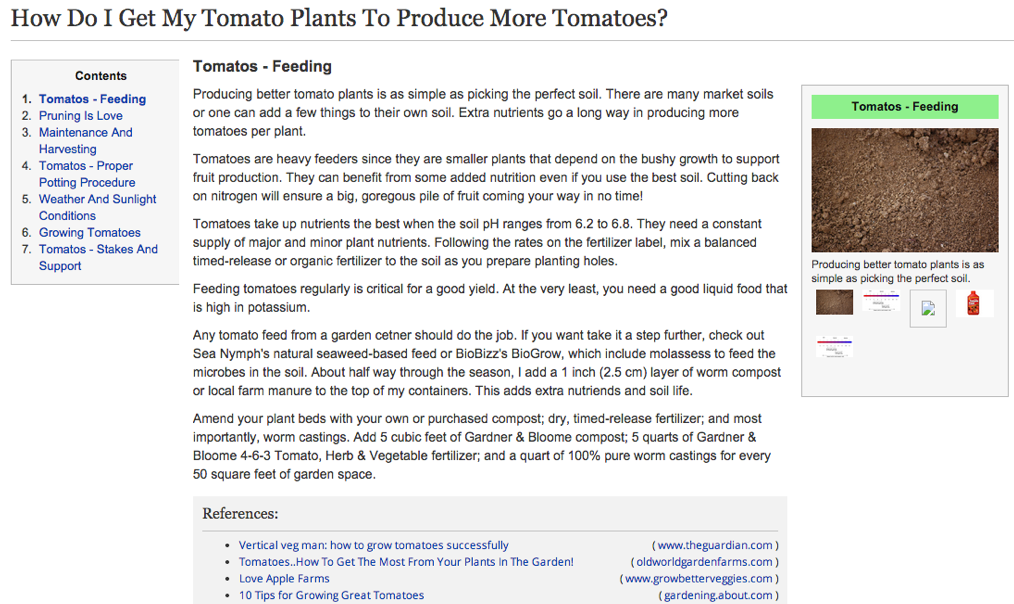
\includegraphics[width=1\columnwidth]{Chapters/KA/final_answer}}
    \caption{The final output of the Knowledge Accelerator system.}
    \label{fig:final_answer}
\end{figure*}
%\michelle{does the description of the task warrant its' own section? not sure... you've probably debated this already and decided this is the best approach, but it seems like at this point, you could skip to the contributions paragraph without needing the info about the task and put a section about the specific situation after?}



\subsection{System Overview}
The ``Knowledge Accelerator'' (KA) is a prototype system which uses crowd workers each contributing small amounts of effort to synthesize online information for complex and/or open-ended questions. The KA system starts with a given question (such as ``How do I deal with the arthritis in my knee as a 28 year old'') and crowdsources the generation of a coherent article that synthesizes different sources, viewpoints, and topics found online relevant to answering the question. Critically, the KA system accomplishes this process without a core overseer or moderator. 

As the goal of the system was to probe how to accomplish a complex information synthesis task entirely through relatively small contributions, we limited our maximum task payment to \$1 US, aimed at incentivizing a target task time of approximately 5-10 minutes. We chose this approach because a fixed payment amount matches the structure of many microtask crowdsourcing markets (e.g., versus a fixed time period of 10 minutes). While some crowdsourcing markets (such as UpWork or eLance) do support hourly rates and fixed time periods, the double-sided transaction (or ``handshake'') costs in which employers and workers vet each other in such markets would constitute a substantial fraction of the working time we target, and the time scale of projects in such markets (typically measured in hours) do not match well with the time scale of the projects we target here (i.e., minutes).\footnote{One concern could be that \$1 could motivate different amounts of effort across different countries. For all tasks other than sourcing and clipping we limited the pool of workers for our tasks to U.S. workers to control for cross-country currency differences. For sourcing and clipping workers U.S. workers spent an average of 9.72 minutes and 6.89 minutes respectively, while non-U.S. workers spent 8.65 minutes and 8.36, which were not significantly different.} 

An example of the output of the system for the target question ``How do I get my tomato plants to produce more tomatoes?'' can be found in Figure~\ref{fig:final_answer}. To produce this output workers find high value sources from the web (e.g., gardening.about.com), extract the useful and relevant clips of information from them, cluster these clips across sources into commonly discussed topics (e.g., feeding or pruning), and generate an article for each topic that synthesizes the relevant clips into coherent chunks of information while reducing redundancies (e.g., if several sources all mention soil pH range, the article should not include that information multiple times). Workers also find relevant multimedia images and video to illustrate each chunk. Information sources used in the creation of the article are referenced in the final output, and the article is organized by subtopics with the most diverse set of references first (See Figure \ref{fig:process} for the KA process overview). 

Our primary contribution in addressing this task is to further our theoretical understanding of the mechanisms and limitations of accomplishing big picture thinking in small pieces, which may have implications for crowdsourcing systems that aim to do complex cognitive tasks including microtask crowdsourcing \cite{kittur2013future}, peer production communities \cite{kittur2008harnessing}, friendsourcing \cite{bernstein2010personalization}, and selfsourcing \cite{teevan2014selfsourcing}. However, addressing this task may also have intrinsic utility in paving the road for crowdsourced systems that can synthesize complex information from a variety of sources on demand. Such systems may be especially useful for topics not be covered by traditional online sources; examples include low frequency or highly personalized search queries (such as looking for information on a particular medical condition given the person's context including age or other symptoms), topics whose sources are highly unstructured and distributed (such as advice giving on discussion forums), or for information that is inside an organization's firewall (such as for a company's IT support sessions). 

%One interesting example we found was for automative diagnostics questions (e.g., ``2003 Dodge Durango has an OBD-II error code of P440. How do I fix it''), where workers synthesized many valuable but unstructured sources of information in car enthusiast forums into a coherent digest. Compared to two commercially available expert-generated databases we found that the system's topics not only covered the solutions but also added ``long tail'' solutions (such as identifying that if the truck was stored in a barn the code is often triggered by mice nesting in the undercarriage for heat) that were considered valuable additions by automotive experts. In the Evaluation section we compare the system's output to a variety of online sources ranging from expert-generated high-traffic sources (e.g., The CDC website) to unstructured user generated sources (e.g., car enthusiast forums).

Below we discuss the challenges involved in developing the system, particularly focusing on issues central to supporting big picture thinking with workers each seeing only a small part of the whole. We first discuss related work, describe the system architecture, then evaluate the utility of the system’s output versus top online sources across a variety of topics.


%%\subsection{Task Selection}

%%To explore this question we set as our goal creating a Wikipedia-like article on an arbitrary topic with no single task paying more than \$1. Creating an encyclopedia-like digest for a target topic (such as how to fix a boiler or what to do about retirement) is an easy to understand task that nonetheless involves several complex and interdependent challenges, including determining a good structure for the article and synthesizing information for different sources into a coherent whole. As we discuss later, the \$1 limit forces the system to avoid bottlenecks where individuals are doing disproportionately large amounts of work.%\niki{I'm not sure what the purpose of this is.  Put here it seems to imply that you could get more value for a dollar by using other workers, but then provides evidence that actually you don't. If it's about addressing the concern that a dollar buys different amounts of work that seems important to have but doesn't seem to fit here; maybe change this to a footnote in the task selection section instead?} 
%%\footnote{One concern could be that \$1 could motivate different amounts of effort across different countries. For all tasks other than sourcing and clipping we limited the pool of workers for our tasks to U.S. workers to control for cross-country currency differences. For sourcing and clipping workers U.S. workers spent an average of 9.72 minutes and 6.89 minutes respectively, while non-U.S. workers spent 8.65 minutes and 8.36, which were not significantly different.} By doing so we aim to further our theoretical understanding of the mechanisms and limitations of accomplishing big picture thinking in small pieces, which may have implications for crowdsourcing systems that aim to do complex cognitive tasks including microtask crowdsourcing \cite{kittur2013future}, peer production communities \cite{kittur2008harnessing}, friendsourcing \cite{bernstein2010personalization}, and selfsourcing \cite{teevan2014selfsourcing}. 


% \jieun {I commented our this sentence and rephrased the previous sentence: Workers identified many valuable but unstructured \jieun{, dialog oriented} sources of information in car enthusiast forums, which the system synthesized into a coherent digest.

\section{Related Work}

\subsection{Crowdwork Complex Cognition and Workflow}

While most crowdsourcing approaches have focused on simple and/or independent tasks, there is a growing interest in crowdsourcing tasks that tap into complex and higher-order cognition \cite{kittur2013future}. Many of these fall into the class of decomposing cognitive processing in a structured way such that many workers can contribute \cite{ahmad2011jabberwocky, bernstein2010soylent, bigham2010vizwiz, kim2014crowdsourcing, kittur2011crowdforge, Kittur:2012:CVM:2145204.2145357, kulkarni2011turkomatic, lasecki2013warping, lasecki2013legion, little2010turkit}. Our work builds on this foundation by incorporating adaptive crowd workflows (e.g., TurKit, JabberWocky, CrowdWeaver), crowd-driven task generation (e.g, CrowdForge, Turkomatic), combining the outputs from decomposed tasks to create a global understanding (e.g., Cascade, Crowd Synthesis) and multi-stage crowd quality control process in which crowds can both generate new versions of output as well as vote on it (e.g., CrowdForge, Soylent, TurKit). However, we go beyond previous work in aiming to support a coherent big picture view while avoiding individual bottlenecks. Doing this is significantly more challenging than the tasks decomposed in prior research, requiring a search for structure during the sampling process, a reliance on novices to function with more context than they enter the task with, and a tight interdependence between each subtask such that any failures could negatively impact the value of the entire artifact. 

\vfill
\subsection{Information Synthesis}

Individual information synthesis is commonly associated with the process of sensemaking. Sensemaking can be characterized as the iterative process of building up a representation of an information space that is useful for achieving the user’s goal \cite{Russell:1993:CSS:169059.169209}. Theories of sensemaking provide a framework for characterizing and addressing the challenges faced by individuals and can point out leverage points for augmenting the process \cite{Russell:1993:CSS:169059.169209,dervin1983overview,klein2006making,karl1995sensemaking, gioia1991sensemaking,daft1984toward,milliken1990perceiving,pirolli1999information}. Generally, models agree that sensemaking is a dynamic and iterative process involving searching for information; filtering that information based on a user's goals and context; inducing a schema or structure from the information; and applying the schema to take action (e.g., writing a report, making a presentation).

A number of systems have been developed aimed at supporting these stages of sensemaking for an individual user \cite{baldonado1997sensemaker, dervin1992mind, dervin1998sense, Marchionini:2006:ESF:1121949.1121979, parameswaran2013datasift, law2011towards} or a group of users working together \cite{kittur2008harnessing, kittur2007he, morris2010wesearch, paul2009cosense, paul2010understanding,karl1995sensemaking}. However, prior research has focused almost exclusively on situations of integrated sensemaking in which individuals (even in groups) are heavily engaged in the entire sensemaking process. Instead, we aim to distribute the information synthesis process across many different individuals, each of whom may see only a limited view of the process.

Computational approaches to parts of the information synthesis process have also been investigated by many researchers. For example, Question Answering (QA) research addresses the methods and systems that automatically answering questions posted by human in natural language. The complex, interactive QA (ciQA) has been introduced at TREC 2006 and 2007 in addition to factoid and list QA \cite {dang2007overview}. However, automated QA approaches (and their crowd-based variants \cite{bernstein2012direct}) focuses on answering short, factual questions instead of the complex sensemaking processes we are interested in, where users build up rich mental landscapes of information.  Another approach is multi-document summarization \cite{barzilay1999information, goldstein2000multi, mani1997multi, mckeown1999towards}, which aims to use computational techniques to extract of information from multiple texts written for the same topic using feature based \cite{gupta2010survey}, cluster based \cite{jain1999data}, graph based \cite{erkan2004lexrank} and knowledge based methods \cite{hahn1999knowledge}. However, such approaches have limitations in dealing with complex yet short and sparse data that encountered on the web, and do not yet engage in the complex synthesis humans perform, which results in the cohesive and coherent output.

%Our approach addresses collaborative information foraging and sensemaking from a unique perspective of using distributed crowd workers alongside machine learning techniques. Compared to the above mentioned scenarios, crowd workers are characterized by easy accessibility, non-expert knowledge, and a limited amount of time to spend on one task \cite{kittur2013future}. Rather than having a completely algorithmic solution, we use a combination of human computation and automatic synthesis to produce a cohesive and coherent output.

\begin{figure*}
    \centering
    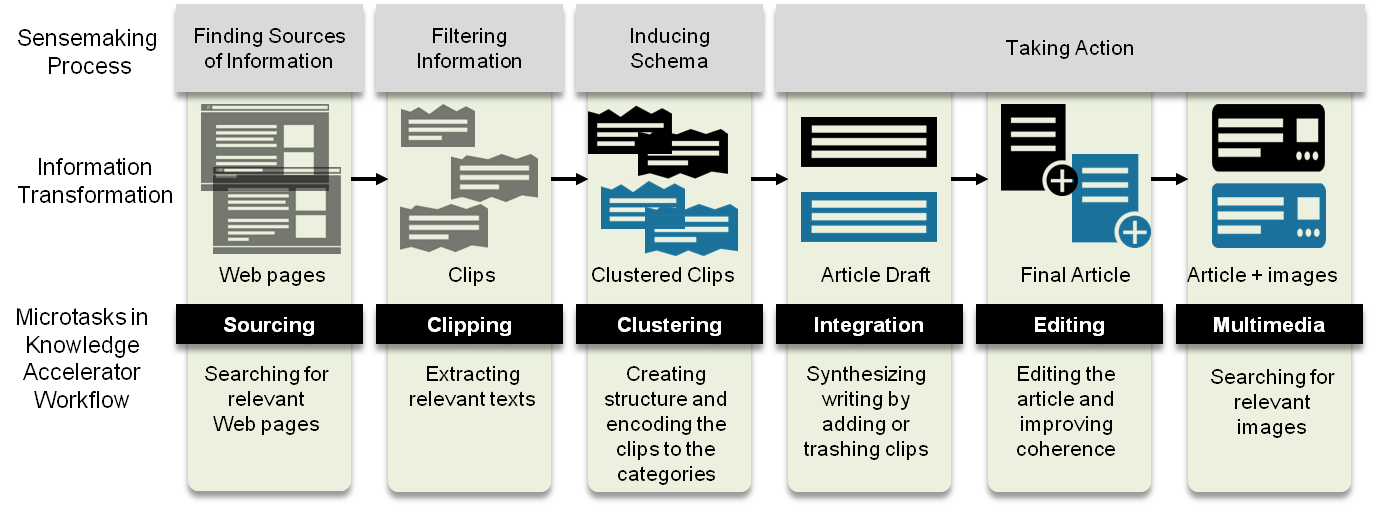
\includegraphics[width=1\columnwidth]{Chapters/KA/overview}
    \caption{The process of the Knowledge Accelerator (KA), from start to finish}
    \label{fig:process}
\end{figure*}

\section{System Architecture}

%The ``Knowledge Accelerator'' (KA) is a prototype system which uses crowd workers each contributing small amounts of effort to synthesize online information for complex and/or open-ended questions. The Knowledge Accelerator system starts with a given question (such as ``How do I deal with the arthritis in my knee as a 28 year old'') and crowdsources the generation of a coherent article that synthesizes different sources, viewpoints, and topics found online relevant to answering the question.

%Critically, the KA system accomplishes this process without a core overseer or moderator. \niki{I think this is the part we should remove / consolodate with intro} The aim of the system was to probe how to accomplish a complex information synthesis task entirely through relatively small contributions. We operationalized this intention by limiting our maximum task payment to \$1 US, aimed at incentivizing a target task time of approximately 5-10 minutes. We chose this approach because a fixed payment amount matches the structure of many microtask crowdsourcing markets (e.g., versus a fixed time period of 10 minutes). While some crowdsourcing markets (such as UpWork or eLance) do support hourly rates and fixed time periods, the double-sided transaction (or ``handshake'') costs in which employers and workers vet each other in such markets would constitute a substantial fraction of the working time we target, and the time scale of projects in such markets (typically measured in hours) do not match well with the time scale of the projects we target here (i.e., minutes).

%An example of the output of the system for the target question ``How do I get my tomato plants to produce more tomatoes?'' can be found in Figure~\ref{fig:final_answer}. To produce this output workers find high value sources from the web (e.g., gardening.about.com), extract the useful and relevant clips of information from them, cluster these clips across sources into commonly discussed topics (e.g., feeding or pruning), and generate an article for each topic that synthesizes the relevant clips into coherent chunks of information while reducing redundancies (e.g., if several sources all mention soil pH range, the article should not include that information multiple times). Workers also find relevant multimedia images and video to illustrate each chunk. Information sources used in the creation of the article are referenced in the final output, and the article is organized by subtopics with the most diverse set of references first (See Figure \ref{fig:process} for the KA process overview). 

%The above tasks of finding, filtering, organizing and generation can be though of as two larger steps: learning a good structure for the article based on sampling information from different online sources, and developing a coherent digest given that structure. To learn a structure workers find high quality online sources and clip relevant pieces of information, which are clustered into topics or categories. The information for each topic is then synthesized into a coherent digest through two steps: first integrating information within a topic, and then enforcing consistency across topics. Below we discuss the challenges involved in developing the system,  particularly focusing on issues central to supporting big picture thinking with workers each seeing only a small part of the whole. We then evaluate the utility of the system’s output versus top online sources across a variety of topics.

%\michelle{at this point, I feel like I'm missing a general overview of what exactly happens... then we have the challenges that all kind of fit together but I don't have a good structure put them into. I guess the figure kind of does this, but possibly a list in the text with a little more description would help me out} \niki{good point. nathan can you add back in a concise 2-3 sentences getting across the essence of the process, maybe noting that we are taking the stages from sensemaking but doing them in a breadth-oriented instead of an iterative way?  i'd suggest putting that description right before this paragraph}\niki{actually cancel that, i'll work on restructuring this whole part to address this better}

Broadly, there are two hard problems involved in crowdsourcing information synthesis: learning a good structure for the article based on sampling information from different online sources, and developing a coherent digest given that structure. Below we discuss how the system addresses each of these problems in turn.

%To learn a structure workers find high quality online sources and clip relevant pieces of information, which are clustered into topics or categories. The information for each topic is then synthesized into a coherent digest by integrating information within a topic, and then enforcing consistency across topics.


\subsection{Inducing Structure}

How can a crowd learn a good structure for an article on an arbitrary topic? Previous crowd approaches such as CrowdForge or CrowdWeaver \cite{kittur2011crowdforge, Kittur:2012:CVM:2145204.2145357} required workers to decide on a structure up before collecting information on each of these topics. However, these approaches fail when the structure must be learned from the data. For example, few workers will know what the subtopics should be for fixing a Playstation’s blinking light or for dealing with arthritis; instead, the appropriate structure should emerge from the data. A single individual making sense of a topic often engages in an iterative process of sampling data and building a structure; however, to reduce the latency of having multiple cycles we explore an alternate approach in which the crowd samples a large amount of data in parallel, then leverage a novel hybrid crowd-machine approach that clusters information into topics without requiring any one worker to see the whole picture.

%induce a structure from that.  a lot of data, use  we first employ crowd workers to find and filter relevant online information. However, as this can collect more information than a single worker could process, we introduce a hybrid

%Research on how people make sense of information online for themselves as they learn new subjects suggests that people go through an iterative sensemaking process in which they are continually finding information about a subject and inducing or refining a structure from the information they found [cites]. Previous approaches such as CrowdForge and CrowdWeaver \cite{Kittur:2012:CVM:2145204.2145357, kittur2011crowdforge} have done a variation of this by having workers decide on an information structure up front, such as what topics should go into an article about New York City (e.g., attractions, economy, etc.), and then other workers search for information on each of these topics. 

%However, it appears that if structure is induced too soon from too few pieces of information, the resulting structure tends to be more poorly formed than if a rich set of information is first collected. Additional research suggests that instead of deciding on a set of topics first and then seeking information for them, one should first seek information and then decide on the set of topics based on what that information contains. Basing the structure on a larger set of online sources has multiple potential advantages: increased coverage of topics, reduced impact from lack of worker prior knowledge (as the knowledge is coming from the sources), and knowledge of which topics are common across many sources (perhaps indicating importance or widely shared viewpoints). For example, in the Playstation scenario described above workers may encounter many possible solutions they wouldn’t have prior knoweldge of, and be able to see which solutions seem to be more commonly cited which might suggest trying them first over solutions that are only mentioned by a single source.

%While there may be multiple benefits, the challenge of crowdsourcing the "seek first - structure later" approach is that much more information is collected for the structuring phase than an individual might easily process at once. Splitting this information up so that each worker only sees a small piece can lead to problems with coming up with good structure; for example, a worker in the above Playstation example might see a solution talking about overheating and, without context of the other solutions, categorize it under overheating. However, if they were to have a global overview of the information, they would know that all the solutions talk about overheating, because that is what the actual problem, and a better category would be the solution type. 

%In a crowdsourced version, workers may not know what the topics should be and the structure of the resulting structure will be missing important topics or focusing on less important topics. For example, in writing an article about approaches to fix a Playstation 3’s blinking yellow light, while there is much information available online about the subject most workers will have little prior knowledge on which to base their judgments of what to include in the article and how it should be structured.

%We describe an approach to addressing this problem below, in which crowd workers first search for and filter information to generate a rich set of data, then a hybrid crowd-machine approach enables clustering the information into topics without having any one worker seeing the whole picture.

\subsubsection{Finding Sources}
To search for and filter high quality information sources we asked five workers to each provide the top five web pages relevant to the target question. We found these numbers to work well in practice; future work using optimization approaches \cite{Kamar:2013:LET:2484920.2485011} could potentially set these dynamically. To ensure high quality responses, for each source we asked workers to report the search term they used and provide a small text clip as ``evidence'' showing why the source is helpful. This approach appeared to be successful in encouraging workers to find high quality sources: workers made on average 2 different queries ($\sigma = 0.3$), and their more commonly cited sources covered more categories of the structure with fewer sources than choosing sources using standard information retrieval approaches (i.e., using the MMR diversity-based re-ranking algorithm to reorder the sources gathered from the crowdworkers \cite{carbonell1998use}). Sources cited by at least two workers were sent to the filtering stage.


%This requires them to browse through each of the sources to gain more understanding of the context, and also encourages them to reformulate their searches to find better sources. 

%Initially, we considered using just the top search results for a particular question as the input for the structure induction stage. However, because we wanted to collect a diverse set of sources, we thought that crowd workers given the ability to perform their own queries might discover a better article set. We conducted a preliminary study where we used the MMR diversity-based re-ranking algorithm to reorder the sources gathered from the crowdworkers \cite{carbonell1998use}, to see if we could cover as many categories extracted in the structuring phase with fewer sources. However, results showed that the original order ranked by crowdworker citation count still covers more categories with fewer sources, indicating that crowdworkers are using good queries and providing valuable judgements when picking sources from the their search results.

%From our experiments, crowdworkers use an average of 1.98 queries ($\sigma = 0.288$) to find the five sources, and find sources that provide more categories with fewer sources than standard information retrieval approaches.

\subsubsection{Filtering Information}

%Each source could contain a variable amount of information relevant to the target question. Some long pages may have very many chunks of relevant information that would exceed the capacity of a single of our tasks, while other pages of the same length may have only a few.  
To filter relevant information snippets from each source workers were presented with one web page and asked to highlight and save at least five pieces of information that would be helpful for answering the question using an interface similar to that described in \cite{kittur2013costs} (Figure~\ref{fig:clipping}). One challenge we encountered was that each page could contain a variable amount of useful information, with some long pages having more snippets than a single worker would extract. To spread out worker coverage on long pages, we showed workers sections that had been highlighted by previous workers and asked them to first look for unhighlighted areas when choosing clips. This preference for novelty and surfacing prior workers' effort allowed us to engage multiple workers for tasks with an unknown amount of relevant information in a more efficient way than simply letting loose many independent workers who would overly focus on the beginning of the page, or having some workers start at the beginning and others at the end \cite{bernstein2010soylent}. To focus more effort on potentially rich sources the system dispatches two workers to each source with an additional two workers for every two additional citations a source received.

\begin{figure}[!ht]
    \centering
    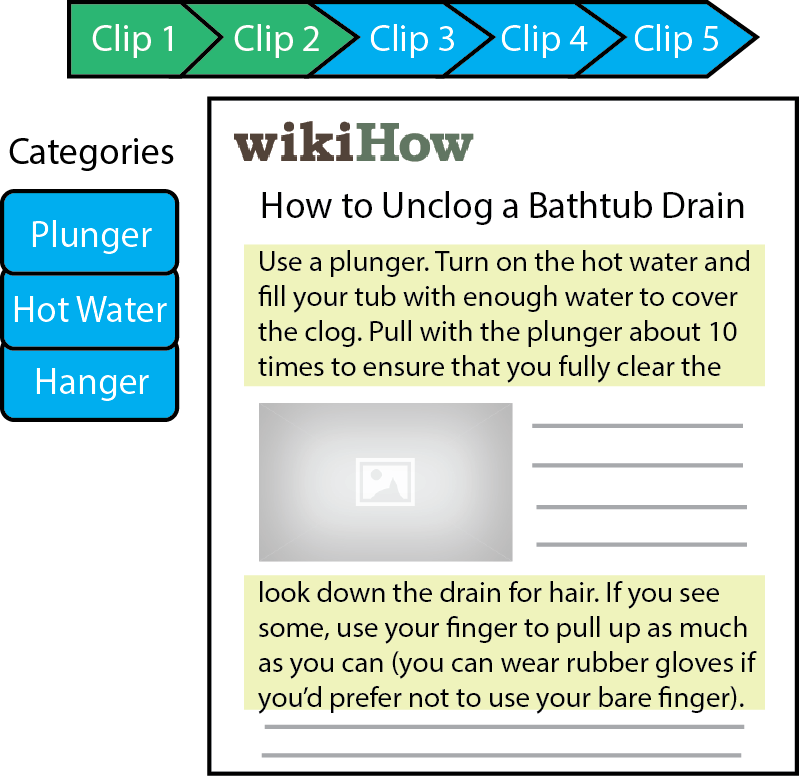
\includegraphics[width=0.5\columnwidth]{Chapters/KA/clipping}
    \caption[Crowdworkers extract and label information from webpages]{Workers extract 5 different pieces of relevant information from pages and give it a label}
    \label{fig:clipping}
\end{figure}

%Sources cited by at least two workers were sent to the clipping phase, where workers extracted from them useful and relevant clips . 

%The idea behind this is that multiple sources will contain overlapping solutions, and in later stages we want to synthesize information for the same solution across different sources. 

%One challenge was maintaining the distribution of information, making sure popular sources are sure to have enough information extracted from them, while still ensuring that a large variety of information is captured. Previous solutions, like "find-fix-verify" \cite{bernstein2010soylent} use a large number of crowd workers and variance for coverage. Instead, to address this, two clipping workers were dispatched initially to any source that reached this citation threshold, with an additional two workers dispatched for every two extra citations a source received. Each worker was presented with one web page and asked to highlight and save at least five pieces of information that would be helpful for answering the question using an interface similar to that described in \cite{kittur2013costs}. To spread out worker coverage on long pages, we showed workers sections that had been highlighted by previous workers and asked them to first look for unhighlighted areas when choosing clips.

Initially we had workers provide labels to categorize each clip, which we planned to use to develop a structure for the article. However, the lack of context of the bigger picture made these labels poorly suited for inducing a good structure. For example, in Figure~\ref{fig:delayed-structuring} the top box shows the category structure induced from labels generated during clipping, while the middle and bottom boxes show the structure induced from the subsequent clustering phase and from a gold standard developed by two independent annotators with access to all clips and sources, respectively. Categories induced from the clipping labels poorly match the gold standard, and include categories with very different abstraction levels (e.g., \textit{Use Drano Max Gel} vs \textit{tips}). This motivated the development of the subsequent clustering phase.

%During this saving process, the worker was prompted to supply a category label for each piece of information they saved. These labels were used only as a work check to control the quality of the clips due to the limited context that each worker had while creating them. Initially, we had planned to use these labels as a way to categorize information for later stages. However, the lack of context of what future clips would be made caused early clip workers form providing labels that ended up serving as poor organization structures. This then caused low quality categories to propagate as new workers used them. This problem aligns with previous research on taxonomy cascades \cite{kittur2014standing,kittur2013costs}, suggesting that we should delay structuring in order to effectively find the proper categories, which motivated the development of the structuring phase described next.

 \begin{figure}[!ht]
 	\fbox{ \vbox{
 		\ttfamily
 		\footnotesize
 		
		\textbf{categories induced during clipping:}\\
 		Boil Water, use hot water, Plunger, try a snake, How to Remove drain stopper, bleach, Use Drano Max Gel, baking soda, drain, tips to unclog, problem, tools, research, internet research, ..., etc.
 		
 		\rule{\columnwidth}{0.1pt}
 		
 		\textbf{categories induced after clipping:}\\
 		Hot Water, Plunge, Plunger, Snake the Drain, Remove the Drain Cover, Drain Cleaner, Remove Hair Clusters.
 		
 		\rule{\columnwidth}{0.1pt}
 		
 		\textbf{annotator categories:}\\
 		Hot Water, Plunger, Plumbing Snake, Remove Cover, Chemicals, Bent Wire Hanger, Call a Plumber, Shop Vacuum.
 	}}
 	\caption[Categories induced from different stages of KA.]{Categories induced from different stages for Q1: \textit{How do I unclog my bathtub drain?}}
 	\label{fig:delayed-structuring}
 \end{figure}

%To demonstrate the difference in category quality during vs. after clipping, in Figure~\ref{fig:delayed-structuring}, we show 1) categories generated by crowdworkers during clipping, where each crowdworker can create new categories or reuse categories created by other workers, 2) categories created after the clipping phase and with the structure induction phase, and 3) categories created by two independent annotators who had access to all the clips and their original sources. The categories generated during clipping are of very different abstraction levels (e.g., \textit{Use Drano Max Gel} vs \textit{tips}), while categories generated after the clipping phase are more coherent and more consistent with the expert categories.

%\begin{figure}[!h]
%    \centering
%    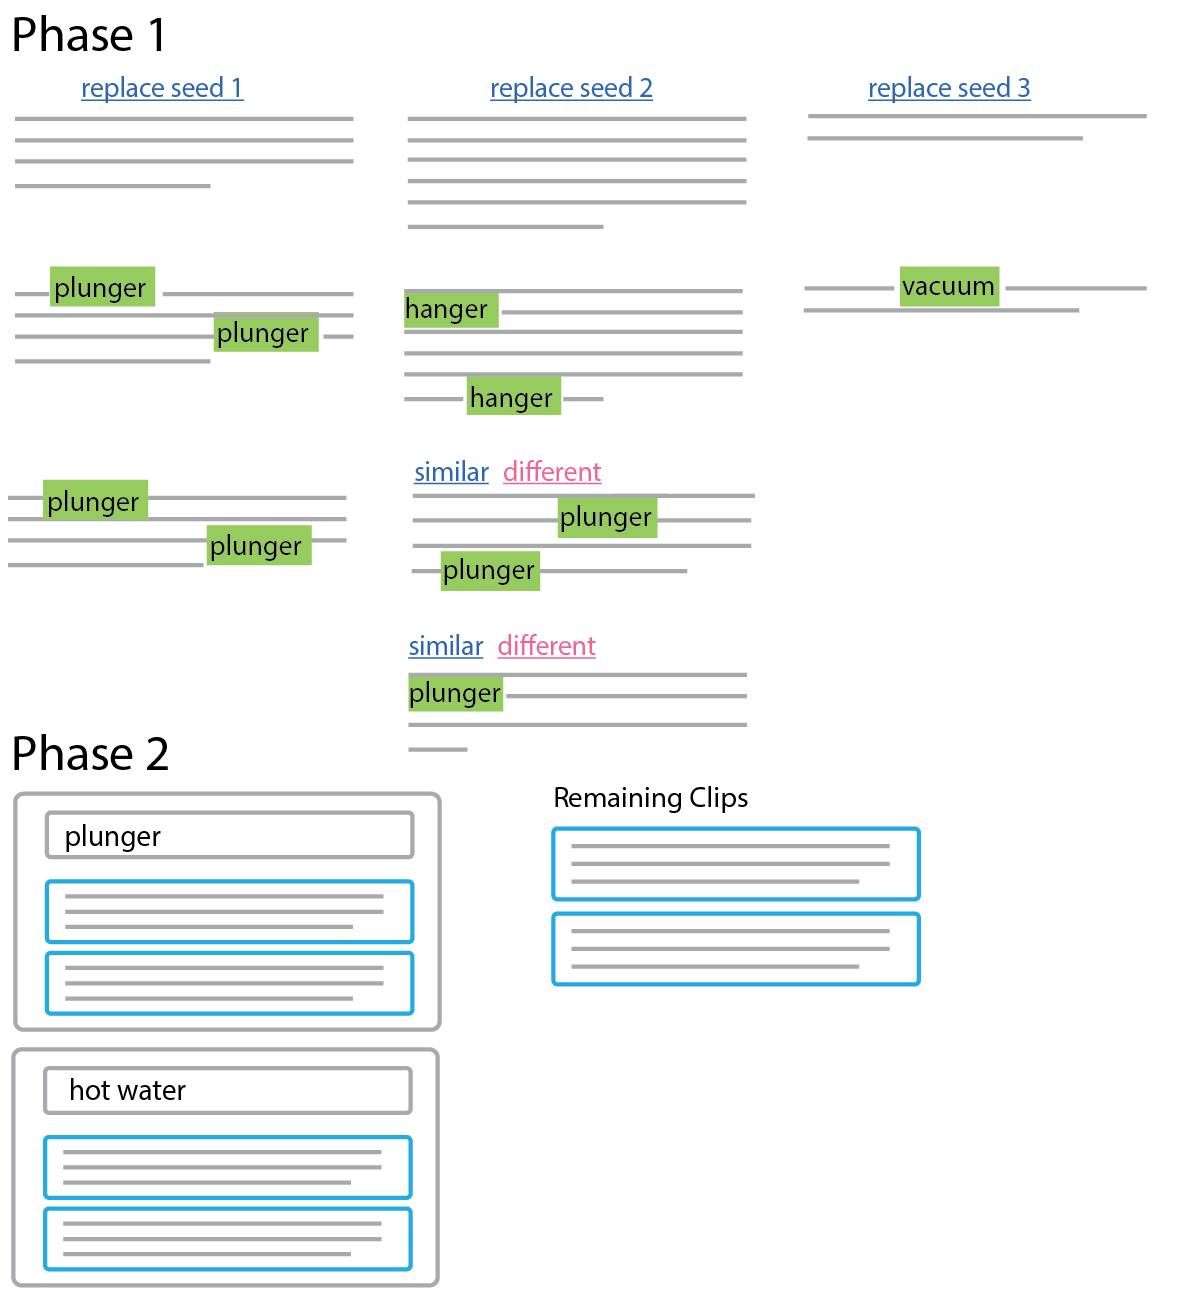
\includegraphics[width=0.9\columnwidth]{clustering-02}
%    \caption{In phase 1 workers identify different seeds and keywords to used in automatic clustering. In phase 2, workers clean up the clusters and name them.}
%    \label{fig:clustering}
%\end{figure}
\subsubsection{Clustering}

%The structuring phase takes all of the clips produced from the clipping phase and tries to extract a categorical structure from them. The motivation behind this is so we can 1) synthesize overlapping information across sources, 2) present the user with different solutions as article sections, and 3) generate smaller sets of clips of the same category so that they are more manageable in the later synthesis stages. The challenge here differs from most crowd-based systems where the tasks can be naturally broken down into smaller pieces, such as labeling images with predefined classes. 

Inducing categories in unstructured collections of text typically requires understanding the global context in order to identify categories that are representative of the information distribution and at appropriate levels of abstraction. The problem of inducing structure without any single worker having a full global context is a particularly challenging problem, and although we describe a basic solution to the problem here for reasons of space and scope, we present a more sophisticated distributed approach in \cite{alloy} that further generalizes the problem to other domains.

%(Figure~\ref{fig:clustering}). 
Our approach takes advantage of the fact that many real world datasets have long-tailed distributions, where a few categories make up the bulk of the head of the distribution and many categories with few instances make up the tail. The intuition behind our approach is that first, the crowd can act as a guide to identify the large categories in the head of the distribution, with their judgments training a classifier to categorize the easy cases with high confidence. After automated classification, the crowd can again be used for ``clean up'', covering the low-confidence edge cases in the tail of the distribution. This also has the added benefit of easily breaking up the larger question context into sub-contexts for easier consumption in the later parts of the system. 

In the first phase, we use workers to label a number of representative categories and leverage those labels to identify meaningful features for an automated classifier. One critical challenge is that workers need to obtain a sense of the distribution of the data without seeing it all. To accomplish this we developed a design we call open-ended set sampling in which workers are presented with four random clips as seeds, and are asked to replace them repeatedly with another random clip until they can determine that the four seed clips belong to meaningfully different categories. Therefore, not only do they have to read the information present in the initial seed clips, but they also need to sample multiple times to understand what ``different topics'' mean for this dataset. In doing so they are randomly shown new clips, which means they are more likely to encounter categories with probability matching the distribution of topics in the data (i.e., higher probability of encountering larger categories).

After workers pick the seeds, we ask them to highlight discriminative keywords in each of the seed clips which are used to query for similar clips from the full dataset, which the workers then label as as \textit{similar} or \textit{different}. With the keyword highlights and the labels created by the workers, we use an SVM classifier and hierarchical clustering to cluster the high confidence portion of the dataset, sending the uncertain instances to Phase 2. 

%One important pattern embedded in the above design is that we leverage worker choice in order to find the clips and keywords that can strongly distinguish between clusters. We accomplish this by indicating to workers that they will have to find similar clips to their initial seed clips, which encorages them to pick good keywords because it helps them reduce their own future workload.

In the second phase, we employ crowdworkers to clean up the output of the classifier, by presenting them the existing clusters on the left of the screen, and the remaining clips on the right. The workers are first familiarized with the clusters by asking them to review the clips in each cluster and give it a short description. They then categorize the remaining clips into existing clusters or create new clusters if no existing cluster is relevant. These categorization judgments are used to refine the hierarchical clustering model.

%This process of evaluating then acting ensures the workers have some understanding of the current context first, so that they can assign clips to the most suitable category, and also to create coherent categories if they need to.

\subsection{Developing a Coherent Article}

%After having induced a structure for the question, there are several possibilities for using the information. For some purposes (e.g.,  \cite{Chilton:2013:CCT:2470654.2466265, kittur2014standing}), it would be enough to just report the categories and associated clips. However, there are benefits to having an article, such as easier consumption, a coherent flow of information, and the inherent organization of information that might not be present in a cluster of short clips.

%The previous section described how to take an online topic area and develop a big picture of its structure through only local views. The output of this process is a set of topics and a set of clips for each topic. 

In this section we describe a set of processes which take as input a set of topics and clips for each topic and output a coherent Wikipedia-like article. There are two core challenges in doing this: first, creating coherence within a topic (e.g., consolidating redundant information); and second, creating coherence between topics (e.g., maintaining consistency across sections). 
%First, we achieve within topic coherence by having individuals integrate the pieces of information within a topic. Second, we have individuals edit the flow of each topic to improve its consistency and coherence with the other sections. 

\subsubsection{Integration}

Within a single topic, there may be many clips which all contain substantively identical information (e.g., the ideal pH level of soil for growing tomatoes); one goal is to reduce this redundancy so that the final article only describes this information once. At the same time, we recognize the value to seeing that multiple sources all say the same thing; thus, we would like to keep track of all the sources that mention a particular chunk of information. Furthermore, tracking source provenance allows the user to drill back to the original information source in case it is described inaccurately or in a biased way.

To accomplish this we developed an interface in which workers were presented with 5 random clips of information for a given subtopic and asked to integrate that information into a shared text pad. Specifically, they were asked to write the gist of the clip in their own words and transfer the provenance of the clip as a footnote. Missing footnotes triggered a verification check.

Initially, we just instructed individuals to cluster similar items together and insert only the footnote for redundant information. However, we noticed that workers were reluctant to change what they perceived as another worker’s contributions, consistent with the social blocking found in Andre et al. \cite{andre2014effects}. This developed into a larger challenge: How could we get workers to gain an understanding of what was in the existing shared pad and feel comfortable modifying it? We introduced a technique we call evaluate then act that requires individuals to read what others have already put into the integrated answer before they are allowed to make a decision about the clip. Our final interface prompts workers to provide specific line numbers corresponding to existing information relevant to their clip, or to explicitly mark their clip as new information or trash. Compared to a version of the system without this structure, significantly more clips were inserted into the middle of the pad to align better to their given section (13\% more, $t(24) = 2.568$, $p < 0.05$) or excluded (11\% more, $t(24) = 4.592$, $p < 0.01$) when workers were asked to evaluate before acting.

%The biggest challenge faced in doing so was encouraging workers to engage in the cognitively demanding task of mapping their clip's information to the information already in the pad, which might include functionally the same information content but in different forms. 
%One challenge with removing redundant information is a relatively subtle but ubiquitous social factor in crowd work: that workers are wary of interacting with other workers’ contributions. [territoriality in wikipedia, difficulty in getting workers to interact and edit each others’ work in andre-limerick writing]. 

\begin{figure}[!ht]
    \centering
    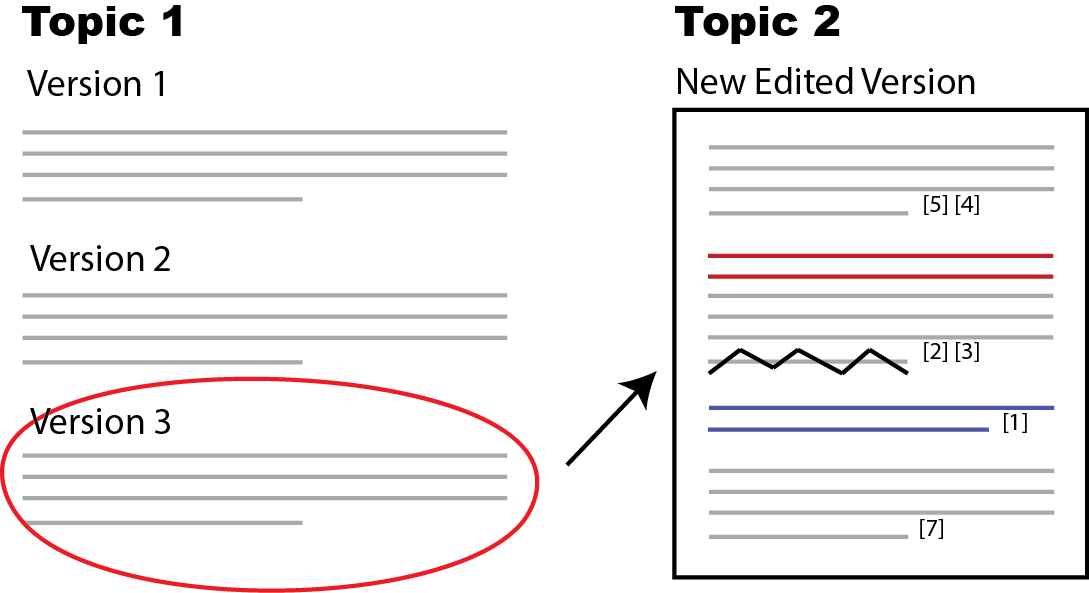
\includegraphics[width=0.6\columnwidth]{Chapters/KA/edit}
    \caption[The 'vote-then-edit' pattern promotes consistency and motivates workers.]{Editing uses the 'vote-then-edit' pattern to promote consistency and motivate workers}
    \label{fig:editing}
\end{figure}

\subsubsection{Editing}

We also noticed that coherence needed to be managed not only within topics, but between topics as well. A number of between topic inconsistencies became apparent during the development process, ranging from formatting to structuring to prose. For example, some topics would be organized with bullet points versus paragraphs, and some in the second person point of view versus third person. Previous crowdsourcing approaches have trouble dealing with cross-topic consistency because reading even a single topic can take significant time, let alone reading and editing across all topics. For example, CrowdForge's \cite{kittur2011crowdforge} approach simply concatenates topics into an article without any attempt at maintaining global coherence. This approach can succeed if the topics and structure either do not require consistency or if they are extremely well specified beforehand: in CrowdForge and CrowdWeaver defining a science article “template” with clear sections such as \textit{what is the problem, what the researchers did}, accomplishes this effectively in a similar manner to core editors specifying a structure in Wikipedia that peripheral members then fill in \cite{kittur2008harnessing}. However, in the general case such well-defined and pre-specified templates are not always available.

%The decision to \textbf{delay structuring} of the Integration task created the need for a task to make the output cohesive and error-free.  Instead, workers would often place their contributions next to existing contributions leading to redundancy (despite instructions to remove redundant text). On average, about 36\% ($\sigma = 0.261$) (using word Levenshtein distance) of the initial pad was modified during editing, suggesting that substantial portions of the pad still merited revision. Another challenge was making each subtopic consistent with other subtopics, as the Integration phase kept each subtopic independent.

To address this we introduced a new pattern which we call vote-then-edit (Figure~\ref{fig:editing}). This pattern asks workers to first review and vote on and choose the ``best'' version of a subtopic created by previous workers, while simultaneously getting a sense for commonalities in style, grammatical choices, and organization. They proceed to edit a new subtopic (phase one) or improve on the item they voted on (phase two). In the second case, we expected workers would more carefully select the best version to reduce their future workload, as well as be more motivated to fix issues in it because they had a choice in what they wanted to do. 

We used the vote-then-edit pattern in an interleaved ``horizontal'' and ``vertical'' workflow. The horizontal phase uses the refined and edited versions of a subtopic section as a ``model'' for improving the rough output from the integration phase for another subtopic section. Specifically, three workers vote on which of three versions of an edited subtopic section is the best and then edit a different subtopic subsection using their answer from voting as a model. Their resulting edited output is sent to the vertical phase, in which three workers vote on which of those versions is the best, and are then asked to further improve this now with all of the other subtopic paragraphs presented to them, to ensure the current subtopic has good flow with the other sections. The output from these workers is used in a new horizontal phase, and the cycle continues.  The intuition here is that the horizontal phase provides only a single section as a model since there is substantive editing work remaining that requires relatively limited context, while the vertical phase provides all sections because the primary editing work remaining is ensuring consistency across sections. Splitting editing into two interleaved phases with different context-work tradeoffs appeared to be more effective than an older editing approach with a single phase. When we compared the evaluation ratings for the older editing to the interleaved vote-then-edit approach for two questions (Q1 and Q2 in Table \ref{tab:evaluation} respectively), the newer answers were found to be significantly more understandable ($\bar{x} = 0.457$, $p < 0.01$) and helpful ($\bar{x} = 0.373$, $p < 0.05$), suggesting this design pattern helped to create more coherent output.


%Therefore, we had two challenges: ensuring a consistent format between sections, and creating a global article flow from topic to topic. Editing was divided up into two phases to tackle these problems separately: an initial editing phase where a worker revises the output from the integration task, and a subsequent consistency phase where individuals are tasked with making the output coherent with other subtopics. In the first phase, a worker votes on the output of a different subtopic's editing phases to choose the ``best'' version. They then are presented with a different subtopic section and asked to improve it, using their answer from voting as a model. In the second phase, individuals vote on the output from the first phase, and are then asked to further improve this now with all of the other subtopic paragraphs presented to them, to ensure the current subtopic has good flow with the other sections. The output from these workers is then used in a different subtopic's first phase, and the cycle continues. This workflow, which we call vote-then-edit (Figure~\ref{fig:editing}), forces workers to read through another topic, and have a sense for its style, grammatical choices, and organization. Additionally, we expected individuals would more carefully select the best version to reduce their future workload, as well as be more motivated to fix issues in it because they had a choice in what they wanted to do. We compared the evaluation ratings for the older editing to the newer editing using this approach for two questions, the bathtub question and the tomato question (Q1 and Q2 in Table \ref{tab:evaluation} respectively) . The newer answers were found to be significantly more understandable ($\bar{x} = 0.457$, $p < 0.01$) and helpful ($\bar{x} = 0.373$, $p < 0.05$), suggesting this design pattern helped to create more coherent output.

\subsubsection{Multimedia}

Images and video can help the reader skim and digest information quickly, as well as provide rich information such as diagrams, instructions, and how-to examples. In our system we enable multimedia from diverse sources to be tied to information blocks, which we define as sections of text demarcated by footnotes. Informally, information blocks correspond to units of information, such as steps in a how-to, or statements or evidence. This has the benefit of ensuring that the images found are specific to pieces of information found in the answer, rather than just being general to the subtopic. For the version of KA described here we did not employ redundancy or voting in the multimedia stage as we did not encounter quality issues; however, since multimedia enrichment is not a particularly interdependent task existing known quality control approaches such as redundancy and voting \cite{kittur2013future} would likely be sufficient for a production system.

\section{Design Patterns}

As mentioned in the above task descriptions, during our iterations on each stage we ended up introducing several design patterns that improved the output. Each phase had its own distinctive challenges, yet they still suffered from some of the core challenges highlighted by previous work: motivation, quality-control, and context \cite{kittur2013future}. Our design patterns served to guide our final system design and add to the set of crowd patterns introduced by previous research \cite{kittur2011crowdforge,bernstein2010soylent,kittur2013future,little2010turkit,bigham2010vizwiz,lasecki2012real,kulkarni2011turkomatic}. They may be particularly relevant for challenges involving complex interdependent tasks requiring global context for workers seeing only local views. 

\subsection{Context before Action}

One of the biggest challenges in crowdsourcing a complex, interdependent task such as information synthesis is providing workers with sufficient global context to perform well despite them having only a local view. Previous researchers have suggested a variety of useful patterns related to this goal, including making the cost of spurious answers as high as valid ones \cite{kittur2008crowdsourcing}, identifying and surfacing specific sub-task dependencies \cite{kulkarni2012collaboratively,retelny2014expert}, unified worker interfaces \cite{zhang2012human} and re-representing tasks in simplified forms \cite{andre2014crowd,Kittur:2012:CVM:2145204.2145357}. We contribute a set of patterns adding to this literature, specifically focusing on a key tradeoff: given a limited amount of time and effort for an individual worker, how can we provide workers with global context (i.e., investing in their ability to make better decisions) but also engage them in actual production work? Too much invested time providing context reduces the amount of time available for improved task performance.

%One of the primary decisions we had to make was how much context we should provide to workers at each step , and how to convey that context to workers in a meaningful way. 

%In the topic identification and clustering phase, there are three different implementations of this pattern. 

\textit{Open-ended Set Sampling.} One challenge with large datasets is giving workers a sense of the distribution of the data despite their observing only subsets of it. This pattern involves a comparison task in which workers are asked to sample random items from the data in order to create a set of non-matching items, as seen in the first step of clustering. A key design factor in this pattern is having a good set function that provides a driver for open-ended sampling and also a stopping point (e.g., when a worker's familiarity with the distribution gives them a sense that their four seeds represent substantively different topics in the dataset).

%\textit{Signal By Doing} In order to get workers to understand the context provided to them, we designed evaluation mechanisms at the beginning of their main task that would both allow them to gain a procedural understanding of their task as well as process the context information produced by other workers. This was a particularly useful pattern, seen in the clustering, integration, and editing phase. In integration, workers had to process previous information in a very specific way so they would both do a specific procedure as well as understand what other workers had done. In editing and clustering, workers had to do a smaller, context-priming task (voting and labeling, respectively). 

\textit{Evaluate then Act.} In order to get workers to understand
the context provided to them, we designed evaluation mechanisms
at the beginning of their main task that would allow
them to get acquainted with the output from previous workers.
This helped workers understand how previous workers
processed the information provided to them, improving consistency
of the output on parallel tasks, and reducing repeated
information. This pattern was leveraged in a number of tasks: clustering, integration, and editing. In the integration phase, we
additionally used the evaluation phase to signal to workers that removing others' work was acceptable and expected, showing that it could be useful in socializing workers into desired procedural practices as well as providing them with context.

\subsection{Tasks of Least Resistance: Leveraging Worker Choice}

Since workers were mostly dealing with dense textual information on a topic they were likely unfamiliar with, we wanted to ensure they were sufficiently motivated. Therefore, we developed a pattern that doubled as both a quality control measure, we well as an incentive for workers. The ``task of least resistance'' pattern requires that the same crowd worker be involved in two stages of the task, a first stage in which they choose what to work on from a number of alternatives (e.g voting) and a second stage in which they themselves benefit from their choice in terms of having to do less work, easier work, or being able to submit a higher quality output. The intuition is that to minimize their later work workers will choose a foundation that requires the least amount of work possible; i.e., they will choose the ``task of least resistance''. This act of choosing is intended to also provide workers with a sense of agency and purpose, which has been shown to increase task performance \cite{chandler2013breaking, rogstadius2011assessment}. This choice also has the potential to increase task performance through workers trying to avoid cognitive dissonance: since workers have themselves presumably chosen the best quality work to start, poor quality final output could reflect on their own worth \cite{weick1964reduction}. This has a trade off of potentially making tasks longer, more complicated, and more expensive, however the benefit is a higher quality output. 

%\subsection{Capturing a Distribution}

%An important part of information synthesis is gathering enough diverse information, while still noting what information is commonly considered to be "better". This is akin to a capturing a distribution: you need to understand which information is more popular, however you need to make sure to still gather the tail information as well. This is not just an issue with information synthesis, understanding distributions is a problem in other domains such as [X, Y, Z]. With enough sampling with crowds, eventually you obtain the desired distribution. However, in order to accomplish this more efficiently, we assign workers for a preference for information novelty and only once the most novel information has been noted, do they recapture the more popular information. This, coupled with assigning more individuals to more "popular" informational sources, creates a biased sampling process that captures all of the information, and then selects a limited portion of the head of the distribution to really promote. 

\section{Implementation}

The main portion of the application was built using Ruby on Rails and integrated with Amazon's Mechanical Turk through the Turkee ruby gem \cite{turkee}. The Ruby on Rails application served as the primary user interface for both the question asker, crowd worker, as well as the answer viewer. A question posed to the system would start the workflow, beginning with source finding. For each stage, after a certain set of conditions were met (number of sources, clips, completed clustering, etc.), the next task in the workflow was automatically started. This allowed the system to run through the entire process with minimal intervention. 

The clipping task utilized Readability's parser API to simplify the appearance of the sources provided during the sourcing phase. This allowed workers to view a cleaner interface in which to clip from, and it also removed some technical limitations involved with clipping from pages that might be multi-paged (readability combines these into one long document) or featured heavy javascript functionality that would interfere with the clipper tool. 

For the first phase of the structure induction tasks, the TfIdfSimilarity ruby gem is used for searching clips similar to the seed clips \cite{rubytfidf}. LIBSVM is used for combining the crowd judgments and cluster a large portion of the dataset \cite{chang2011libsvm}. For the integration and editing tasks, we utilized the Etherpad-lite text pad library \cite{Etherpad} to allow workers to simultaneously work on the same output.

\section{Evaluation}

To evaluate the usefulness and coherence of the system's output we compared it to sources an individual might use if they were to complete this task without the KA system. This would most likely involve the use a search engine such as Google to gather information and use existing information sources to learn about the topic. Therefore, as an evaluation, we had a separate set of crowd workers perform a pairwise comparison of the KA output to that of top results returned by Google and those found useful by multiple crowd workers.

\subsection{Method}

Participants were recruited through the AMT US-only pool and paid \$1.50 for the evaluation task. Each participant was randomly assigned to compare the output from the KA system with an existing top website for that question. An individual could only provide one rating per question, but could do the rating task for more than one question. We removed 34 of the 1385 unique participants who provided an evaluation rating who also participated in a KA system task.

The ``top websites'' used in the comparison task were the top five Google results, as well as any additional Google results that were highly cited (mentioned by 3 or more turkers) during the sourcing phase of the system. Some questions had a larger number of highly cited sources, resulting in more additional websites, as can be seen in Figure~\ref{fig:aggregated}.

In the evaluation task, participants were first asked a series of questions that would cause them to read and understand both sources. In order to encourage quality through defensive task design \cite{kittur2008crowdsourcing}, for the output from the KA system and the existing web page, they were asked to list the different sections on each and three different keywords that would describe those sections. After they read and parsed each web page, they were presented with a brief persona of a friend who was having the problem posed to the KA system. Workers were then asked, for that problem, to rate the comprehensiveness, confidence, helpfulness, trustworthiness, understandability, and writing of each web page on a seven point Likert scale (from 1 to 7) and provide an explanation for their rating on each dimension. We averaged ratings on these dimensions into a single score representing the overall perceived quality of the page.

We selected 11 target questions for evaluation by browsing question and answer forums, Reddit.com, and referencing online browsing habits \cite{pewReport}. For some questions, we added some additional constraints to test the performance of the system for more personalized questions. In addition to this external evaluation, we also had the crowdworkers who participated in the KA system fill out a short feedback form detailing their experience using the system. We ask three questions about the difficulty of the task, the clarity of the instructions provided, and the easy of use of the user interface. We recorded some brief demographics about our workers, including to the country they were from.

\begin{table}
  \centering
  \footnotesize
% question, number of sources, number of clips, number of turkers
  \begin{tabular}{l r l}

	Question &
	\multicolumn{1}{c}{N} &
    \multicolumn{1}{c}{Score} \\
    \hline
	% 102
	\multicolumn{1}{p{0.75\columnwidth}}{\textbf{Q1}: \textit{How do I unclog my bathtub drain?}}
	& 116 & ~0.292 * \\

	% 115	
	\multicolumn{1}{p{0.75\columnwidth}}{\textbf{Q2}: \textit{How do I get my tomato plants to produce more tomatoes?}}
	& 177 & ~0.420 * \\

	% 153
	\multicolumn{1}{p{0.75\columnwidth}}{\textbf{Q3}: \textit{What are the best attractions in LA if I have two little kids?}}
	& 158 & -0.044 \\

	% 116
	\multicolumn{1}{p{0.75\columnwidth}}{\textbf{Q4}: \textit{What are the best day trips possible from Barcelona, Spain?}}
	& 98 & -0.109 \\

	% 177
	\multicolumn{1}{p{0.75\columnwidth}}{\textbf{Q5}: \textit{My Worcester CDi Boiler pressure is low. How can I fix it?}}
	& 139 & ~0.878 * \\

	% 168
	\multicolumn{1}{p{0.75\columnwidth}}{\textbf{Q6}: \textit{2003 Dodge Durango has an OBD-II error code of P440. How do I fix it?}}
	& 138 & ~0.662 * \\

	% 175
	\multicolumn{1}{p{0.75\columnwidth}}{\textbf{Q7}: \textit{2005 Chevy Silverado has an OBD-II error code of C0327. How do I fix it?}}
	& 135 & ~0.412 * \\

    % 160
	\multicolumn{1}{p{0.75\columnwidth}}{\textbf{Q8}: \textit{How do I deal with the arthritis in my knee as a 28 year old?}}
	& 139 & ~0.391 * \\

    % 161
	\multicolumn{1}{p{0.75\columnwidth}}{\textbf{Q9}: \textit{My Playstation 3 has a solid yellow light, how do I fix it?}}
	& 119 & ~0.380 * \\

    % 162
	\multicolumn{1}{p{0.75\columnwidth}}{\textbf{Q10}: \textit{What are the key arguments for and against Global Warming?}}
	& 138 & ~0.386 * \\

    % 163
	\multicolumn{1}{p{0.75\columnwidth}}{\textbf{Q11}: \textit{How do I use the VIM text editor?}}
	& 138 & ~0.180 \\
    \hline
    \multicolumn{3}{l}{\textbf{*} = significant at $p < 0.01$ after Bonferroni correction}\\

  \end{tabular}
  \caption[Comparing KA output with top websites for the eleven questions.]{Average difference between the KA output and top websites for the eleven questions (positive indicates higher ratings for KA, negative indicates higher ratings for the competing website). Each rating was an aggregate of 6 questions on a 7-point Likert scale.}
  \label{tab:evaluation}
\end{table}

\begin{figure*}
    \centering
    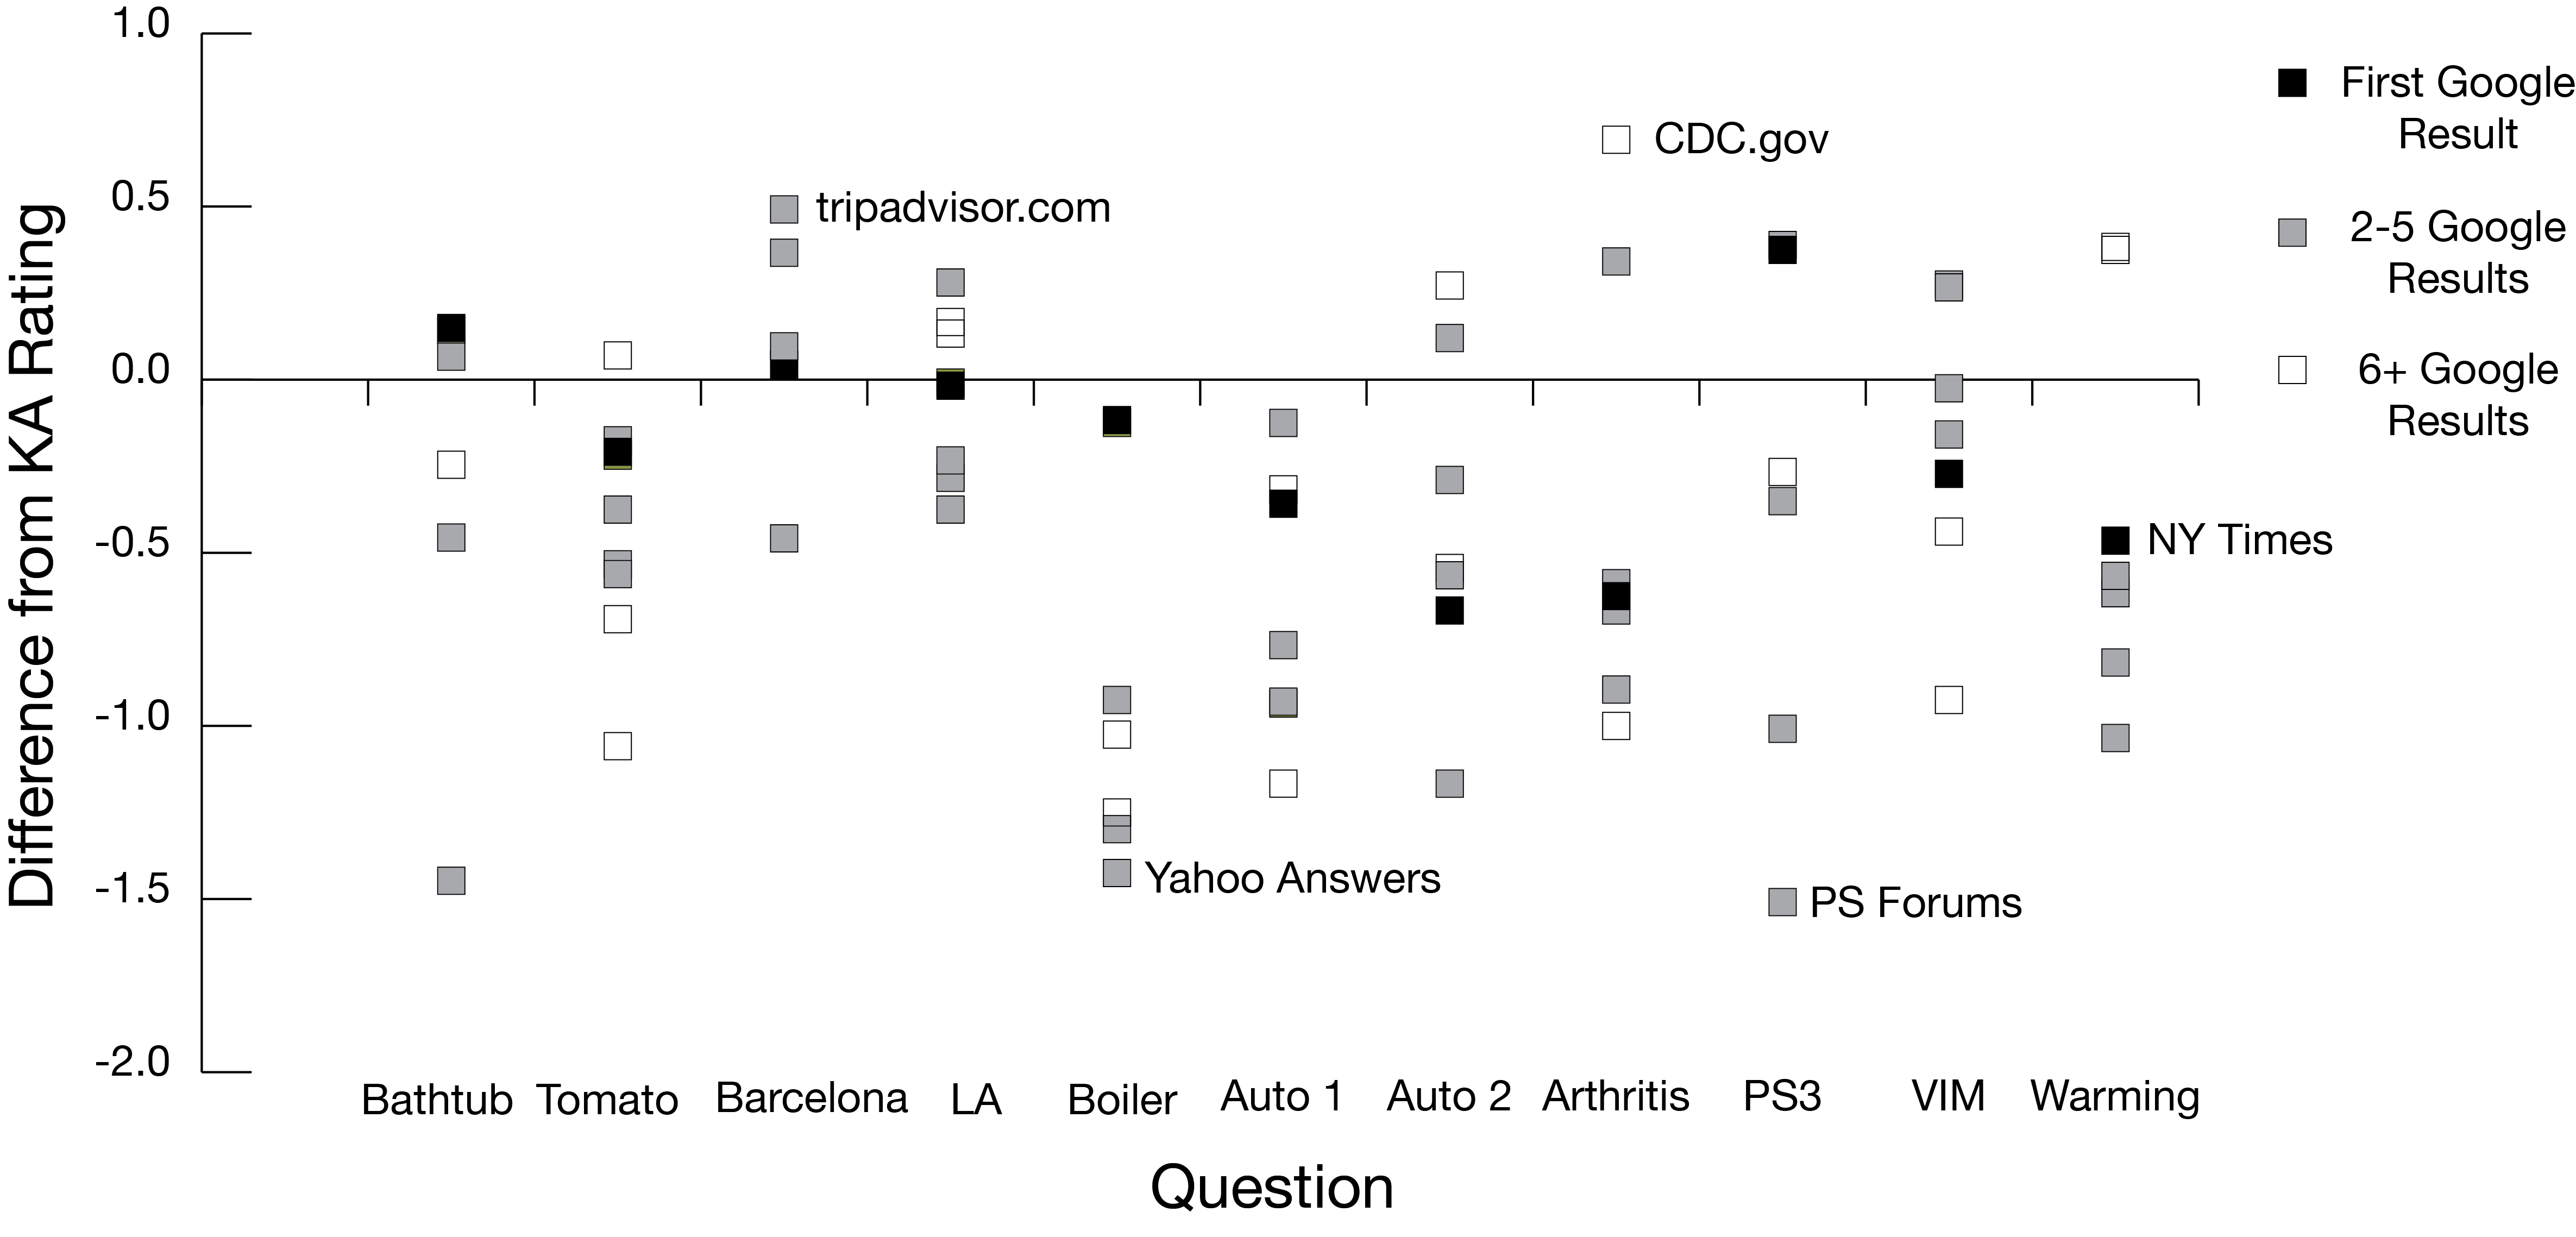
\includegraphics[width=1\columnwidth]{Chapters/KA/source_eval_graph}
    \caption[Results across questions and websites.]{Results across questions and websites. Points represent the average aggregate score difference between the KA answer and an existing site}
    \label{fig:aggregated}
\end{figure*}

\subsection{Results}
Aggregating across all questions, KA output was rated significantly higher than the comparison web pages, which included the top 5 Google results and sources cited more than 3 times (KA: $\bar{x} = 2.904$ vs Alt. Sites: $\bar{x} = 2.545$, $t(1493) = 13.062$, $p < 0.001$). An analysis of individual questions corrected for multiple comparisons is shown in Table~\ref{tab:evaluation}. 

The strongly positive results found were surprising because some of the websites in the comparison set were written by experts and had well-established reputations. Only on the two travel questions, Barcelona ($\bar{x} = -0.109$) and LA ($\bar{x} = -0.044$), and the VIM question ($\bar{x} = 0.180$) did the KA output not significantly outperform the comparison pages. A closer examination of these pages suggests that for the two travel questions, because of the strong internet commodity market surrounding travel, a considerable amount of effort has been spent on curating good travel resources. Even with the slightly more specific LA query, there were still two specialized sites dedicated to attraction for kids in LA (Mommypoppins.com and ScaryMommy.com). The VIM question represented a mismatch between our output and the question style. A number of the sources for the question were tutorials, however in the clipping phase, these ordered tutorials were broken up into unordered clips, creating an information model breakdown. This points out an interesting limitation in the KA approach, and suggests that adding support for more structured answers (e.g., including sequential steps) could be valuable future work. 

%\begin{figure}
%    \centering
%    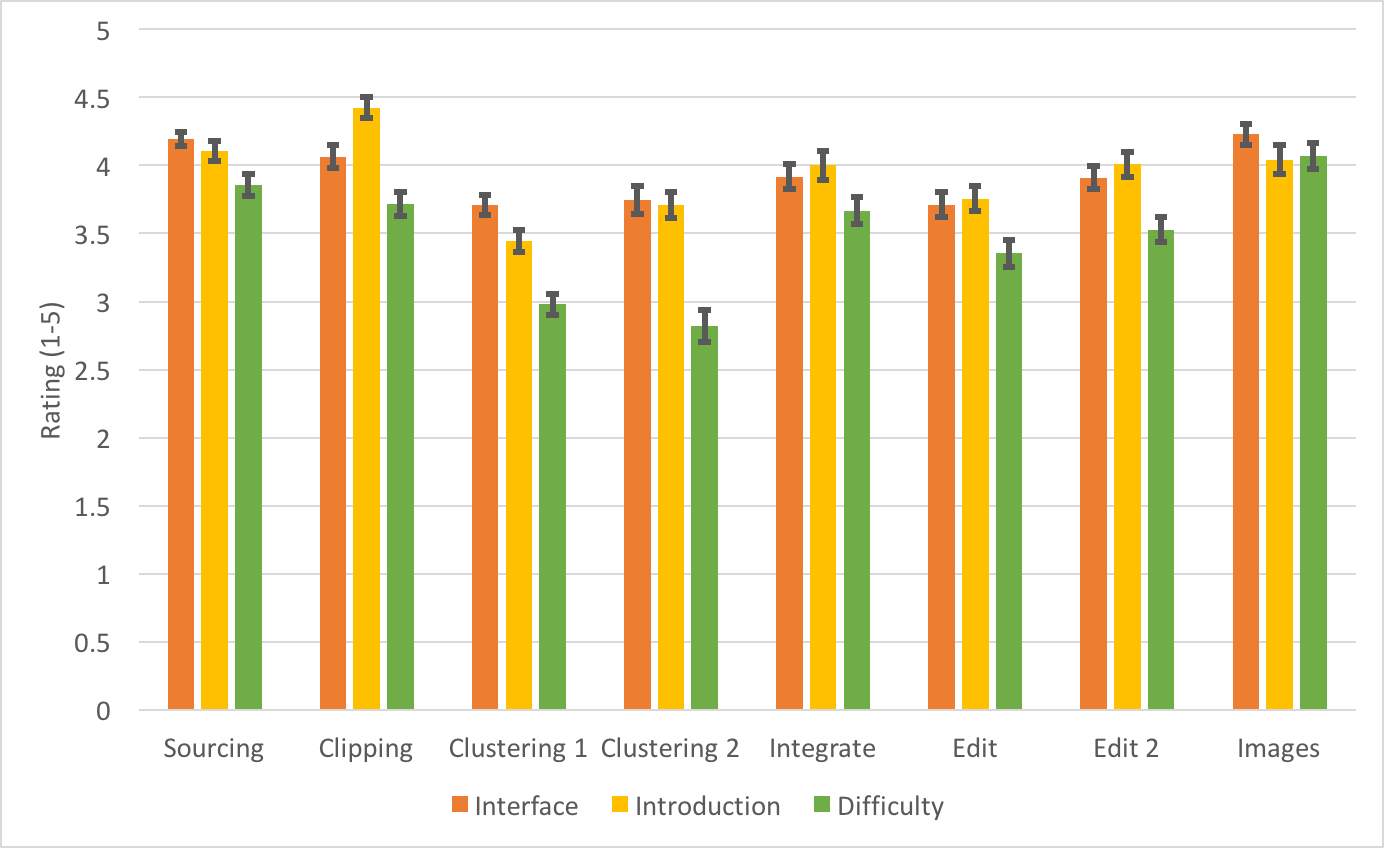
\includegraphics[width=1.0\columnwidth]{feedback}
%    \caption{Difficulty, instructions, and interface ease of use self-report from workers participating in the KA system. A lower number indicates a higher difficulty, poorer instructions, or a difficult interface.}
%    \label{fig:feedback}
%\end{figure}

As an additional external evaluation, for the two questions (Q6 and Q7) related to automotive systems we compared the discovered categories from the KA system with two commercial knowledge service products generated by expert technicians. We compared the KA response's accuracy and comprehensiveness, and found that it discovered all the categories referred to in these two commercial products for each question. Furthermore, the categories from the KA output provided more categories not mentioned in the commercial product (average 2.5 categories from two commercial products, while average 9.5 categories from KA). We validated these additional categories with expert automotive professionals who evaluated them as also being plausible and reasonable for the given questions. There was one instance in which two distinct categories (Encoder Motor and Encoder Motor Sensor) from the commercial products were clustered into the single category named Encoder Motor Assembly in the KA output. However, the full text answer from the KA system for Encoder Motor Assembly did still contain these two sub-components with different repair procedures. 

It may seem surprising that KA would work well for questions such as automotive error codes, where the response relies heavily on technical knowledge and jargon. On further inspection we believe this is because there are many online resources that have valuable information pertaining to these questions but are in unstructured and dialog oriented forms. Workers in the sourcing phase found rich sources of online information from many car enthusiast discussion forums, in which members tried to diagnose and help each other solve their automative problems. Although crowd workers may not understand the esoteric jargon of the automative domain, their understanding of grammar, semantics, and argument structure was sufficient to let them find, filter, cluster, integrate, and edit this domain-specific information. These results suggest a interesting avenue for future research leveraging human understanding of semantics and argument structure to extend crowdsourcing to process expert domain knowledge and to understand the limits of where such an approach breaks down.

%(see Figure~\ref{fig:feedback})

On average, running a question through the KA system cost a total of \$108.50 (see Table~\ref{tab:cost}). Although our primary goal was to establish a proof of concept of accomplish big picture thinking in small pieces, we return to the issue of cost in the Discussion. From the self-report crowdworker feedback, workers mostly found the tasks to be easy to complete, with the clustering phase having the most difficult task.

\begin{table}[ht]
  \centering
% question, number of sources, number of clips, number of turkers
  \begin{tabular}{lrrr}
    \hline
    \textbf{Phase} & \textbf{Task Pay} & \textbf{Avg. \# of Tasks} & \textbf{Avg. Cost} \\
    \hline
	Sourcing & \$0.25 & 15 & \$3.75 \\

    Clipping & \$0.50 & 21.6 & \$10.80 \\

    Clustering 1 & \$1.00 & 10 & \$10.00 \\

    Clustering 2 & \$1.00 & 10 & \$10.00 \\

    Integrate & \$0.50 & 37.2 & \$18.60 \\

    Edit 1 & \$0.75 & 28.8 & \$21.60 \\

    Edit 2 & \$1.00 & 28.8 & \$28.80 \\

    Images & \$0.50 & 9 & \$4.50 \\
    \hline    
    \textbf{Total} & & 160.4 & \$108.05 \\
    \hline
  \end{tabular}
  \caption[Average number of worker tasks and cost of running KA.]{Average number of worker tasks and average cost per phase, and overall, to run a question.}
  \label{tab:cost}
\end{table}
%The most notable result was the difference in output for different question types. Ideally, any question posed should be answerable by the system. However, the KA system appeared to do significantly better for some types of questions, while it was mediocre, or worse, for other types of questions. Therefore, we think the KA system is very effective for questions that fall on the "long tail" of search queries \cite{bernstein2012direct}. The output from the KA system, for any question, might be considered acceptable, and that acceptableness shines when the other available sources are poor or too general. Questions 5 through 10 show this, as those questions feature either a modifier to the query e.g Q8's "as a 28 year old" or are specific to a particular product (Q5-7, Q9). 

%Some of the qualitative feedback we received seemed to suggest this as well. For Q3, individuals noted that the message was often ``a lot better conveyed" than the KA output or the competing website was just ``simpler." For Q2 and Q4, raters noted the KA output just ``throws too much information at you" and also the layout made it difficult to read all of the content. However, for Q5-7, many of the raters noted that the sites appeared to be very "unprofessional" and the KA system "actually has useful information about the problem ... [alt website] is filled with questions without answers." 
\section{Discussion}

Our primary goal was to investigate the opportunities and limitations of accomplishing big thinking in small pieces, using a distributed information synthesis task as a probe. We instantiated our design approach in a prototype system called the Knowledge Accelerator which crowdsourced the process under the constraint that no single task would pay more than \$1, and investigated its performance across a variety of complex information seeking questions. Results suggested that the output of the system compared favorably to top information sources on the web, approaching or exceeding perceived quality ratings for even highly curated and reputable sources.

The strong performance of the system is perhaps surprising given that its output was generated by many non-expert crowd workers, none of whom saw the big picture of the whole. We do not believe that this should be interpreted as a replacement for expert creation and curation of content. Instead, the power of the system may actually be attributable to the value created by those experts by generating content which the crowd workers could synthesize and structure into a coherent digest. This explanation suggests that the approach would be most valuable where experts generate a lot of valuable information that is unstructured and redundant, such as the automative questions in which advice from car enthusiasts was spread across many unstructured discussion forums. In contrast, KA's output did not outperform top web sources for topics such as travel, where there are heavy incentives for experts to generate well structured content.  We believe its performance is likely due to its aggregation of multiple expert viewpoints rather than particularly excellent writing or structure per se, though this is a fruitful area for future investigation.

In developing the KA system, we explored a number of approaches that did not work. We initially tried to avoid a clustering phase altogether by exploring variations of the clipping task in which we provided additional context to workers in having them read through multiple sources, engage the workers who found sources in doing the clipping, or have them build on the categories that other workers had already generated rather than work independently.  However, in all cases workers did not generate good labels due to a lack of context. We then explored introducing an additional ``conductor'' view, in which workers could be recruited as clips came in to organize those clips and close categories that had a sufficient number of clips; however, this also failed because the conductors did not have sufficient global context to create good categories. These failures motivated the hybrid crowd-machine clustering phase.

Development of the integration and editing phases also included many false starts due to the opposite problem of giving workers \textit{too much} context. Our first integration interface enabled multiple workers at the same time to easily view and expand all the clips in a category for within-category context, and also see the current state of how other categories were developing for between-category context. Our idea was that as workers integrated clips and built out more options exposure to the other clips and options in real time would help them create more coherent digests. However, this approach proved overwhelming for scaling up to a large number of crowd workers engaged for short time periods. This motivated us to split up within-category and across-category consistency into the integration and editing phases and the development of the vote-edit pattern.

We encountered a number of places where our approach could be improved. As evidenced in the VIM question, the lack of support for nuanced structure in our digests can prove problematic. For some sources such as tutorials or how-tos, supporting sequential dependencies between steps could be useful. While our output was able to support such dependencies in an ad-hoc way within a category (such as the sequential steps for plunging a drain) it would be profitable to be able to support sequential dependencies across categories (e.g., first try x, then try y). More structure could also be beneficial for particular domain areas, such as explicitly capturing symptoms and causes as different types for automotive or medical diagnostic questions.

%Overall the KA system performed well, considering the number of existing curated sources. One of the most interesting results from the evaluation was the different performance for different questions. While initially we attributed this to the KA system only performing well for certain question types, in reality it had to do with the search results. If Google was able to return a large amount of high quality results, such as for a travel question, the KA output was not significantly better. This suggests that the KA system output is very good in most cases, but it's much harder to tell when comparing to other strong articles. This becomes especially apparent in the extremely specialized questions, such as the boiler or automotive questions. 

%While we tried to emulate the individual model of sensemaking, one of the biggest pieces, iteration, is severely lacking from our system. Sensemaking theories \cite{dervin1983overview, dervin1998sense,pirolli1999information,Russell:1993:CSS:169059.169209} agree there is this constant process of searching for information, and improving a mental model based on the gathered information. In online information foraging, this process can be observed in the form of querying a information retrieval engine, learning new knowledge from the search results, and reformulating the next query \cite{Gayo-Avello:2009:SSD:1523512.1523556,Spink:1998:MUS:865316,swanson1977information}. However, in our system, there is only one phase of searching and structuring. 

%We somewhat avoid this due to our delayed structuring design pattern. In individual sensemaking, this is iteration partially due to limitations of working memory and serial processing constraints, as each piece of information is costly in time and storage to consume. In contrast, distributing the information synthesis process across individuals and using computation to help store and cluster information relaxes these constraints significantly. Thus instead of iterating to find a better structure, KA instead casts a wider initial net (which can be done by many workers in parallel) to have better context when doing the structuring. 

The system could also benefit from including iteration. For example, after workers completed the integration phase they were asked the question ``What else needs to be done to make this a complete answer?''. While many obviously said the section needed be edited, one of the most popular responses was ``Needs more information.'' This suggested to us that while our clips and categories had pulled in most of the information, there was more information in some sections we were missing. One possibility is to introduce an iterative component at this point -- as workers are integrating information into the pad and notice missing information, they can request for other workers to go out and find that additional information through clipping. %Another possibility is to introduce iteration earlier during the clustering phase. Individuals could pose questions or missing content areas when reviewing the clusters, prompting a second round of sourcing and filtering for a more refined question.%
Thus while the system was partially successful at taking a breadth-oriented approach rather than the deeply iterative approach typical of sensemaking \cite{dervin1983overview, dervin1998sense,pirolli1999information,Russell:1993:CSS:169059.169209}, understanding how to best incorporate iteration would be a valuable area for future work.

A final area for future improvement is the cost associated with producing answers. Our digests took approximately \$100 to produce. While intended as a proof-of-concept prototype and similar in scale to other such crowdsourcing systems \cite{andre2014crowd,Chilton:2013:CCT:2470654.2466265}, it is interesting to consider what could be done to move the approach towards a useful production system with lowered costs. One area of improvement is optimization: by dynamically deciding how many workers and products to use in each stage final costs could be dropped significantly (e.g., as in \cite{Kamar:2012:CHM:2343576.2343643}). Furthermore, for many practical information seeking purposes the categories and associated clips may be sufficent, which would obviate the need for the expensive stages of integration and editing and reduce costs by over 65\%. 

Perhaps the most interesting possibility is if answers could be reused across questions. Although users have complex information seeking needs, many of the queries they issue are similar. For example, a recent study estimated that 3\% of search queries account for one third of total search volume \cite{white2007studying}. Thus at a minimum, many answers could be amortized across users with the same question. A particularly promising but challenging opportunity is if similar questions may be able to reuse components of already summarized answers; for example, a question on investing advice for a 50 year old might use some common categories as for a 20 year old, but others would be unique to the new question's context. Challenges for the reuse of information are how the system would be able to identify the similarity for possible answers during each information synthesis phase and what level of granularity should be considered to for an effective system. Spatial and temporal reasoning over the existing knowledge and new information could be considered to provide context-aware and up-to-date answers. 

We hope the design choices embodied in the KA prototype system and the design patterns discussed here may be useful for other system designers working to distribute cognitive complex tasks. Some domains that might benefit from this include microtask markets, which could benefit from supporting more complex tasks; volunteer crowdsourcing efforts such as Wikipedia \cite{kittur2008harnessing} or friendsourcing in which many small contributions are readily available \cite{bernstein2010personalization}; or self-sourcing in which the crowd within could accomplish complex tasks in small increments (e.g., waiting for the bus) without needing to load the entire task context into working memory \cite{teevan2014selfsourcing}. Overall, we believe this approach represents a step towards a future of big thinking in small packages, in which complex and interdependent cognitive processes can be scaled beyond individual cognitive limitations by distributing them across many individuals.

%\section{Acknowledgments}

%The authors would like to thank to Andrew Peters for his initial work on the KA system. This work was supported by NSF grants IIS-1149797, IIS-0968484, IIS-1111124, Bosch, and Google.

%\section{Appendix}

%See \url{http://nhahn.org/portfolio/ka.html\#appendix} for additional resources, including the original articles generated by the KA system.

% Balancing columns in a ref list is a bit of a pain because you
% either use a hack like flushend or balance, or manually insert
% a column break.  http://www.tex.ac.uk/cgi-bin/texfaq2html?label=balance
% multicols doesn't work because we're already in two-column mode,
% and flushend isn't awesome, so I choose balance.  See this
% for more info: http://cs.brown.edu/system/software/latex/doc/balance.pdf
%
% Note that in a perfect world balance wants to be in the first
% column of the last page.
%
% If balance doesn't work for you, you can remove that and
% hard-code a column break into the bbl file right before you
% submit:
%
% http://stackoverflow.com/questions/2149854/how-to-manually-equalize-columns-
% in-an-ieee-paper-if-using-bibtex
%
% Or, just remove \balance and give up on balancing the last page.
%


\Chapter{Alloy}{Coherent Categorization with Crowds and Computation}
\label{chap:alloy}

{\rmfamily
This work was previously published in ACM SIGCHI 2016 (\cite{alloy} and\cite{ka}) and has been adapted for this document.
}


%!TEX root = main.tex

% *** What are you trying to do? Articulate your objectives using absolutely no jargon.  What is the problem?  Why is it hard?
% *** How is it done today, and what are the limits of current practice?
%People generally organize complex information by identifying the salient concepts
%and themes that effectively structure the data. However, this process often involves
%a small group of people with deep understanding of the domain and
%access to the entire data in order to discover
%a good structure that is both helpful and coherent.
% From Niki:
% Consequently, unsupervised text processing algorithms
% might fail to recognize the salient features that are crucial to discovering a
% set of good abstract concepts. Crowdsourcing platforms provide a mechanism to
% recruit human computation on demend, which can potentially be the remedy for
% such methods.  However, abstract concept discovery and clustering can be
% timeconsuming and cognitively taxing even for crowdworkers, as they need a
% global understanding of the information-scape to arrive at a good level of
% abstraction.  Further, it can be challenging to provide enough context while
% keeping the microtasks tractable.
% *** What's new in your approach and why do you think it will be successful?


% original, 200 words
%Crowd-based clustering is a new and promising field, because people can make better judgements than machines based on their deeper understanding of the information at hand. However, a global understanding is often required to identify useful categories, and it can be difficult to provide enough information in a microtask. Past work employs the crowd to process arbitrary parts of the dataset, but this lack of shared and global context can lead to incoherent results. This paper describes Alloy, a crowd-based short text clustering workflow that uses a ``\emph{sample and search}'' process to provide context beyond showing a fixed set of items. Alloy also introduces a ``\emph{cast and gather}'' framework that allows it to cast out types of microtasks for different human judgements, and gathers them by using a machine learning backbone to form coherent results. With this framework, Alloy first use the crowd as trainers for a classifier that captures the more prominent clusters, and then use the crowd again as cleaners to capture difficult items and smaller clusters. To evaluate, we clustered Web clippings, Wikipedia discussions, and research papers, finding that Alloy had higher accuracy than machine learning baselines, higher accuracy and increased efficiency compared to crowd-based approaches, and yielded comparable precision to inter-annotator agreement.
% shortened to 150
%Crowd-based clustering is a new and promising field, because people can make better judgements than machines with deeper understanding of the information at hand.  However, it is difficult to provide enough global information in a microtask. Past work divides the input into arbitrary parts, but this lack of shared global context leads to incoherency.  We present Alloy, a crowd-based text clustering workflow that uses a ``\emph{sample and search}'' process to provide context beyond fixed sets of items. Alloy also introduces a ``\emph{cast and gather}'' framework that allows it to cast out  microtasks  for types of  human judgements gathered by a machine learning backbone: First, Alloy uses the crowd as trainers for a classifier that captures the prominent clusters, then uses the crowd again as cleaners to capture smaller clusters. Alloy yielded comparable precision to inter-annotator agreement, outperforming machine learning and crowd-based approaches in accuracy and efficiency.

This chapter describe the first of the two crowd systems in this dissertation that explored ways to provide global context in crowdsourcing. This first system focused on the task of data clustering, a common approach to data analysis. In the domain of crowdsourcing, this typically involves assigning sets of items to different crowdworkers and using human judgements to both creating categories and assigning items under them.
Crowdsourced clustering approaches present a promising way to harness deep semantic knowledge of human computation for identifying coherent categories and clustering complex information.
However, existing approaches have difficulties supporting the global context needed for workers to generate meaningful categories, and are costly because all items require human judgments. We introduce Alloy, a hybrid approach that combines the richness of human judgments with the power of machine algorithms. Alloy supports greater global context through a new ``\emph{sample and search}'' crowd pattern which changes the crowd's task from classifying a fixed subset of items to actively sampling and querying the entire dataset.  It also improves efficiency through a two phase process in which crowds provide examples to help a machine cluster the head of the distribution, then classify low-confidence examples in the tail. To accomplish this, Alloy introduces a modular ``\emph{cast and gather}'' approach which leverages a machine learning backbone to stitch together different types of judgment tasks. In an application-oriented evaluation, Alloy clustered were further synthesized into comprehensive overview articles using a workflow described in \cite{ka}. Results show that Alloy structures can lead to coherent and comprehensive overviews that out performed top Google search results published by experts in scenarios where there are a lack of authoritative sources.

% old framing
% 
% We present Alloy, a clustering approach that
% combines the strengths of human computation with machine learning to cluster complex information. 
% Previous approaches use either crowds or computation 
% have had difficulty dealing with
% high-dimensional data, providing sufficient context, and enforcing global
% constraints.
% To address these challenges Alloy introduces the \textit{cast-and-gather} approach:
% casting out for different types of human judgments which are gathered in a continually-improving 
% machine backbone. This approach enables clustering to be broken into
% multiple phases: one in which crowdworkers identify major clusters in the head
% of the distribution which serve as training for machine to learn item similarity, and another in which crowdworkers classify the sparse and difficult items in the tail.
% To evaluate, we
% clustered Web clippings, Wikipedia discussions, and research papers, finding that Alloy had higher accuracy than machine learning baselines, higher accuracy and increased efficiency compared to crowd-based approaches, and yielded comparable precision to inter-annotator agreement.

%\niki{reframe into key take-away ideas here, e.g., backbone etc}
%First, crowdworkers are employed to recognize the salient
%dimensions and discover abstract concepts for training a machine learning model
%that predicts the similarity between documents. Then, we combine global
%clustering results created by crowdworkers using an iterative clustering
%mechanism that enforces global constraints.  

% Who cares?
% If you're successful, what difference will it make?   What impact will success have?  How will it be measured?
% What are the risks and the payoffs?
% How much will it cost?
% How long will it take?
% What are the midterm and final "exams" to check for success?  How will progress be measured?


\section{Introduction}
%!TEX root = main.tex

\begin{figure}[!ht]
	\centering
	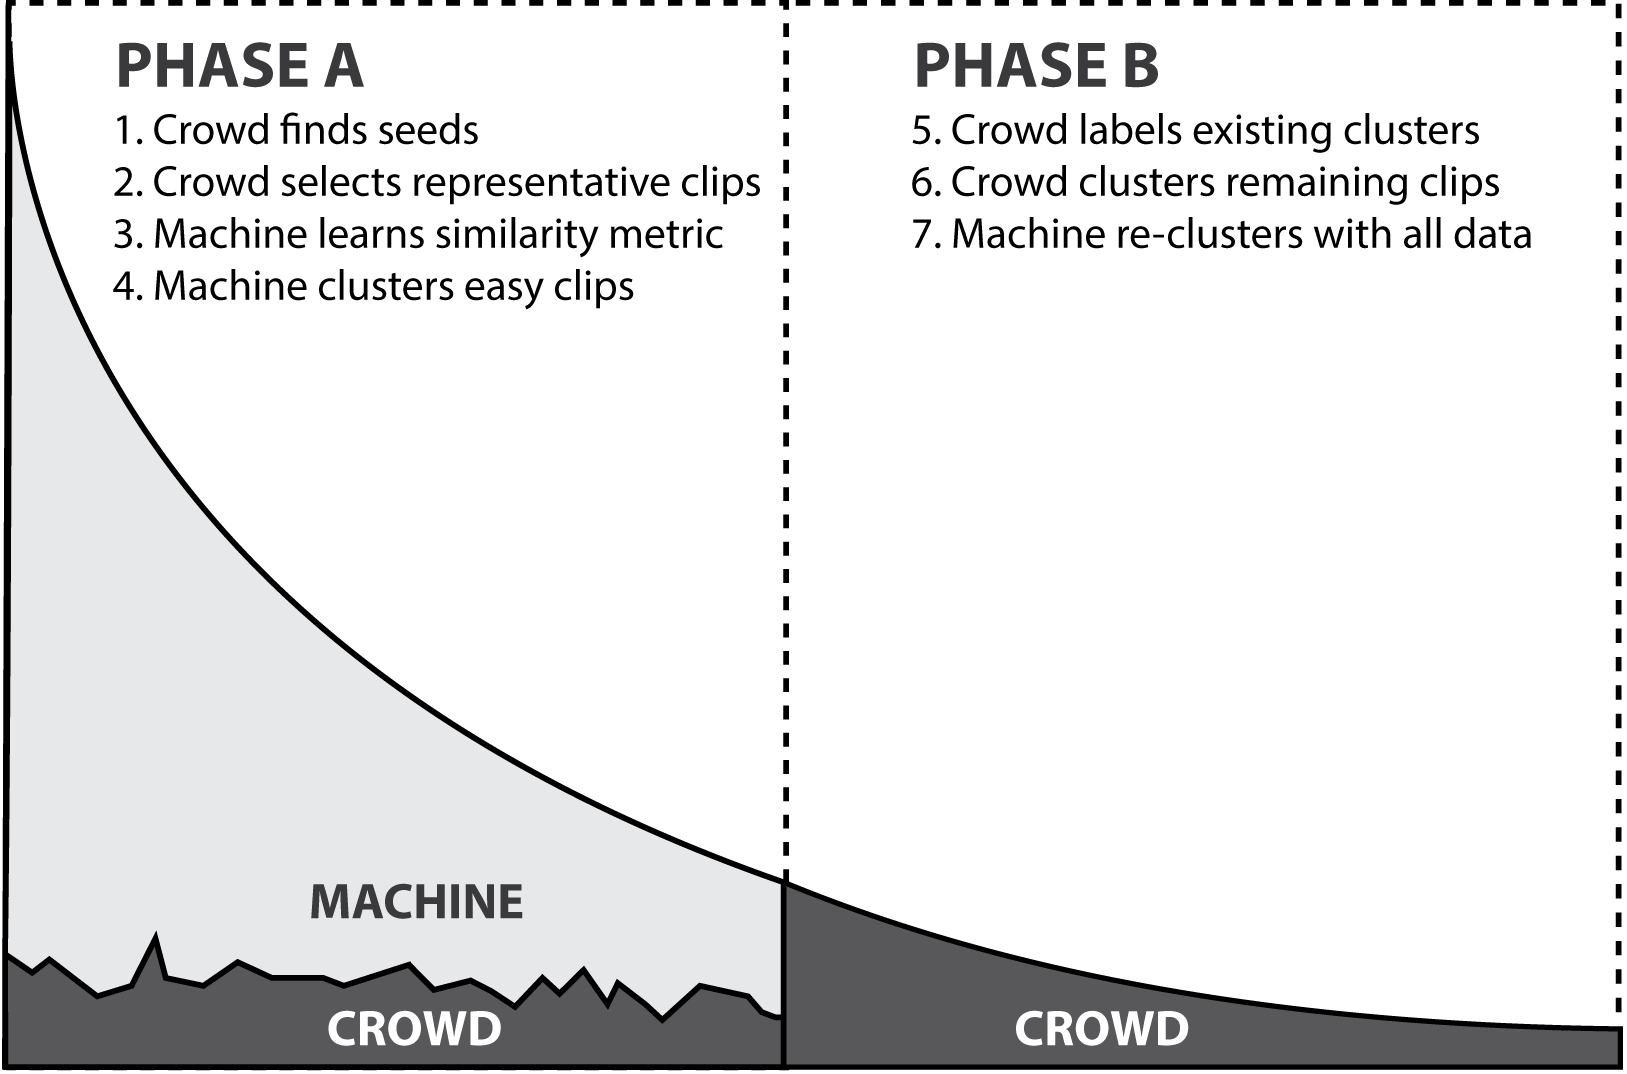
\includegraphics[width=0.6\columnwidth]{Chapters/Alloy/images/alloy_overview_01.png}
%	\caption{First, we use the crowd for creating labels and select features to
%		train a machine learning model. Then, the trained model clusters a
%		large part of the input data.  Finally, the crowd takesover again to
%		refine the output from the machine to produce the final result.}
	\caption[A conceptual overview of the Alloy system.]{
		A conceptual overview of the system. In the first phase, crowd workers identify
		seed clips to train a machine learning model, which is used to classify
		the ``head'' of the distribution. In the second phase, crowd workers classify
		the more difficult items in the ``tail''. A machine learning backbone provides
		a consistent way to connect worker judgments in different phases.
	}
	\label{fig:workflow}
\end{figure}

% - Clustering unstructured information is important, but current machine algorithms have problems understanding deeper semantics of rich textual data. 
% - Recent research has begun to ..., <give examples of current work's success> However, <move examples from related work>.

Clustering, or pulling out the patterns or themes among documents, is a fundamental way of organizing information and is widely applicable to contexts ranging from web search (clustering pages) to academic research (clustering articles) to consumer decision making (clustering product reviews) \cite{jain1999data}.  
For example, a researcher may try to pull out the key research topics in a field for a literature review, or a Wikipedia editor may try to understand the common topics of discussion about a page in order to avoid or address previous conflicts. Doing so involves complex cognitive processing requiring an understanding of how concepts are related to each other and learning the meaningful differences among them \cite{Bellman:2003:DP:862270,kriegel2009clustering,medin1978context}. 

Computational tools such as machine learning have made great strides in automating the clustering process \cite{blei2003latent,chuang2012termite,chaney2012visualizing}. However, a lack of semantic understanding to recognize the important differences between clusters leaves the difficult task of identifying meaningful concepts to the human analyst \cite{chuang2012interpretation}. This reflects an inherent advantage for humans over machines for the complex problem of understanding unstructured data beyond merely measuring surface similarity, and a corresponding opportunity for research in combining human and computational judgments to process complex information \cite{fails2003interactive, Kulesza:2014:SLF:2611247.2557238, hu2014interactive}.

One such promising avenue of research harnesses the power of crowds to identify categories and cluster rich textual data. Crowdsourcing approaches such as Cascade, Deluge, and Crowd Synthesis \cite{chilton2013cascade,bragg2013crowdsourcing,andre2014crowd} have demonstrated the power of splitting up rich, complex datasets into small chunks which can be distributed across many human coders. However, all of these approaches must grapple with a fundamental problem: since each human coder is seeing only a small part of the whole dataset, a lack of global context can lead to incoherent results.  For example, if the items sampled are too similar, the worker might create overly fine-grained clusters. On the other hand, if the items sampled are too dissimilar, the worker might create overly broad clusters. Clusters found in many worker segmentation sets may give rise to redundant clusters, while clusters whose items are sparsely split among segmentation sets may never be realized at all. As an example, \cite{andre2014crowd} cite redundancies in Cascade's top level clusters having both ``green'' and ``seafoam green'', ``blue" and ``aqua'', as well as the encompassing category of ``pastels''. While Crowd Synthesis used an iterative approach to address these redundancy problems, it trades this off with lowered robustness as issues with early workers' categories can cascade throughout subsequent workers' judgments. This suggests the design space of approaches for crowd clustering may be being critically limited by the assumption of splitting up the dataset into small, fixed pieces that prevent workers from gaining a more global context.

Another challenge with current crowd clustering approaches is that using human judgments to label each piece of data is costly and inefficient. Deluge addresses some issues with efficiency, improving on Cascade by reducing the number of human judgments elicited as the rate of new category generation slows \cite{chilton2013cascade}. However, these crowd clustering algorithms still require human judgments for every item, which is costly. In the real world data often follows a long-tailed distribution in which much of the data is captured by a small number of categories in the head of the distribution \cite{white2007studying}. For such data in which many items in the head of the distribution are likely to be highly similar, once humans have identified the meaningful categories and representative examples it would be more efficient if a machine could classify the remaining items in those categories. A danger with such an approach is that the sparse categories in the tail of the distribution with few examples may be difficult to train a machine to recognize, and so human judgments may have another important role in ``cleaning up'' low frequency categories.

%Past work also explored ways to combine expert workers and computation for categorizing unstructured textual information using interactive interfaces \cite{huang2006text,settles2011closing}.
%Both studies showed that using one expert worker to identify a small set of informative keywords can significantly improve the results of machine clustering on the 20 newsgroup dataset, where each category has similar number of articles.
%However, it is also common for a collection of information to be not evenly distributed across topics, but instead follow a highly skewed distribution \cite{white2007studying}. In such cases, statistical based algorithms may perform well on the typical cases in prominent topics of the dataset, but fail to capture the edge cases and the smaller categories. 
%Intuitively, it could be greatly beneficial to use human judgements again to clean up the output, covering cases that are difficult for the machines but relatively simple for people.


%Such advantage is partly based on a good global understanding of the information at hand, which either comes from prior knowledge and/or comprehending the entire dataset for expert workers.
%However, this creates challenges for system designers due to the distributed nature of crowdsourcing \cite{Kittur:2013:FCW:2441776.2441923}, namely the lack of domain knowledge of the workers and the difficulty of providing enough global information in a microtask for finding good categories.
%Since it is infeasible to ask crowdworkers to read all items in the dataset, current work simply employs crowdworkers to process arbitrarily parts of the dataset \cite{chilton2013cascade,andre2014crowd}. 
%This lack of global context can lead to incoherent results, because different workers are creating clusters based on different small pieces of the puzzle. For example, if the items sampled are too similar, the worker might create overly fine-grained clusters. On the other hand, if the items sampled are too dissimilar, the worker might create overly broad clusters. 
%In general, most current systems provide context by showing a small sample of items, hoping that it captures the distribution of information in the larger dataset. 

%People have been developing machine learning algorithms to cluster unstructured rich textual data using similarity measurements based on surface features. However, without deeper semantic understanding of the information at hand, it can be difficult for machines to distinguish which features embody useful categories.
% For example, \emph{sunlight} and \emph{lights} are potentially good features for the first text clip in Figure~3 if other items in the dataset are about ways to better grow tomatoes, but not so if other items are about the seeding of various plants. 
%For example, \emph{liquid water} is potentially a good feature for the second text clip in Figure~3 if other items in the dataset are about key factors of supporting life on a planet, but not so if other items are about the various roadmaps of NASA. 
%Human intellect, on the other hand, is readily able to infer meaningful categories from complex data given enough context  \cite{Bellman:2003:DP:862270,kriegel2009clustering,medin1978context}. This gives crowds an inherent advantage over machines for the complex problem of understanding unstructured data beyond merely measuring surface similarities, and a corresponding opportunity for research in combining crowds and computation to cluster complex information.



% 
% \joseph{new}
% % moded from the info-seeking framing
% Whether researchers, shoppers, students, or voters, a common challenge is
% synthesizing information gathered from multiple sources into
% meaningful and useful categories
% to gain a bigger picture in order to 
% identify the core topics,
% such as specs for a new product, ways to
% unclog a drain, organizing research papers into conference session, or the key issues
% involved in an election. 
% For example, an individual searching for health information may have
% to go to over a dozen web sites in order to get a complete picture of a domain
% \cite{bhavnani2005difficult}. While doing so information seekers aim to
% determine the common themes and the distribution of information across those
% themes, eventually trying to decide which information is important and which sources to
% trust \cite{kittur2014standing}.  This represents a substantial cognitive
% challenge and a corresponding opportunity for research in better supporting
% individuals engaged in these tasks. 

% dont draw attention to scaling
%In this paper, we explore an alternative approach of an ad hoc, crowd-driven
%method for finding structures and organizing %datasets with less than a few thousand items.



% 1. keywords can help machines get much better results
% 2. skew distribution
% 3. machines output still needs human clean up 




% A key difference from previous work on crowd clustering is our two-stage model
% of clustering.
% %There is a conflict between providing sufficient context
% %for identifying categories in a skewed distribution and the limited context capacity of
% %microtasks that are suitable for posting to online crowdsourcing marketplaces such as Amazon Mechanical Turk. Further, i

% In such cases the head of the topic distribution
% contains a disproportionate number of clips, and once a human has labeled a few
% of these clips it is inefficient to continue using human labor to finish
% labeling them as automated methods can do a reasonably good job.  Conversely,
% the tail of the topic distribution contains topics with few clips,
% and expending resources to train a machine learning algorithm to
% identify these sparse topics is less advantageous, while it is comparatively
% easy for humans to classify these clips.

% Previous crowdsourcing research has shown success in using the crowds to capture uncommon cases in a long tailed distribution to improve inline answers in Web search engines \cite{Bernstein:2012:DAS:2207676.2207710}.



% 
% , it can lead to problems
% enforcing global constraints such as redundant or overly similar
% categories, categories at the wrong level of abstraction due to lack
% of context, categories that do not represent the distribution of
% information faithfully because of sampling issues, or simply inadequate categories
% because of worker motivation or expertise issues. 
%
% dont draw attention to scaling
% Furthermore, hiring workers
% incurs monetary costs and thus can have issues scaling to large amounts
% of data compared to computational approaches. 
%
% old framing for "the but"
% Existing crowd clustering approaches have addressed some of these
% challenges, but often with significant trade-offs. For example, 
% methods that are robust against a few poor judgements often fail to enforce global
% constraints, leading to overlapping, incoherent, or duplicated categories. On the other hand,
% methods that focus on producing
% coherent results by providing global view to the crowds are often vulnerable to a few
% poor judgements in early stages cascading through the workflow
% \cite{chilton2013cascade,andre2014crowd}.
%
% 
% This paper describes Alloy, a crowd-based short text clustering workflow that uses a \emph{sample-and-search} process to build up workers’ mental models with context beyond showing multiple arbitrary items.
% We believe this is a new way to support global context for crowd clustering.

% In addition, we introduce a \emph{cast-and-gather} framework that allows Alloy to cast out various types of microtasks for different types of human judgements, and gathers them using a machine learning backbone. With this framework, Alloy 
% incrementally cluster the datasets in a two-phase approach: First, workers actively request for context by repeatedly sampling random items and searching for similar items in the entire dataset while building up their mental model of the global context. Based their labels, a machine classifier then clusters unlabeled items with high confidence, capturing the prominent categories (the head of the distribution). Then, crowdworkers switch roles from trainers to cleaners, capturing smaller clusters and items that are difficult for the machine classifier (the tail of the distribution).

This chapter describes Alloy, a hybrid approach to text clustering that combines the richness of human semantic judgments with the power of machine algorithms. Alloy improves on previous crowd clustering approaches in two ways. First, it supports better global context through a new ``\emph{sample and search}'' crowd pattern which changes the crowd's task from classifying a fixed subset of items to actively sampling and querying the entire dataset. Second, it improves efficiency using initial crowd judgments to help a machine learning algorithm cluster high-confidence unlabeled items in the head of the distribution (prominent categories), and then uses later crowd judgments to improve the quality of machine clustering by covering the tail of the distribution (edge cases and smaller categories). 
To achieve these benefits, Alloy introduces a novel modular approach we call ``\emph{cast and gather}'' which employs a machine learning backbone to stitch together different types of crowd judgment tasks. While we provide a particular instantiation of the cast and gather approach here (with a hierarchical clustering backbone which gathers three types of crowd tasks, or ``casts''), the general framework for modularizing multiple types of human judgments with a common machine-based backbone may inspire application to other contexts as well.


% old framing for the therefore
% 
% We introduce Alloy,
% a new approach to structure complex information by identifying meaningful clusters of short text
% with crowds and computation.
% Alloy is based on the intuition that we
% can employ the crowd to act first as a guide, highlighting the high-level
% structure of a domain as training for a machine learning model; then, after
% the algorithm has classified instances that are easy for it to
% categorize, the crowd can further clean up the results by categorizing the
% remaining instances that proved more difficult. Different from many of the previous
% approaches which gather small and independent human judgements for all
% instances and stitch them together to infer concepts,
% we use a machine learning model to scale crowd judgements to cover unlabeled instances.  
% By using a two phase approach, we try to compensate for the shortcomings of crowdsourcing (e.g., lack of context,noise) and machine learning (e.g., sparse data, lack of semantic understanding) by utilizing techniques from both fields. 
% We focus on providing rich context
% to crowdworkers and transferring context between workers in different phases with a machine backbone algorithm.
% Using this approach we aim to enforce global constraints while
% also leveraging machine learning to increase scalability and to protect against
% poor worker input.

\subsection{Related Work}

%\niki{want to start with a paragraph that sets up the importance of clustering
%    itself and gets to the crowd framing faster. Like the paragraph two down
%    from here. I'd put these two paragraphs later in the intro or in a related
%    work section. Remember that an AC will probably skim the first couple
%    paragraphs to decide who to recruit as reviewers. }

Document and short text classification are well researched topics in natural
language processing and machine learning. With enough labeled training data,
state-of-the-art algorithms can often produce good results that are useful
in real world applications. Yet building such systems often requires expert
analysis of specific datasets both to manually design an organization scheme and
to manually label a large set of documents as training data. Unsupervised approaches, 
or clustering,
aim to discover structures on-demand and without expert preparation
\cite{jain1988algorithms,hartigan1975clustering,steinbach2000comparison}.
While these
data mining approaches may discover dimensions (features) that provide a good
separation of the dataset, the inferred categories can be difficult for a human
to interpret, and many of them may not capture the most meaningful or useful
structure in a domain due to high dimensionality or sparseness in the word vector space 
\cite{Bellman:2003:DP:862270,kriegel2009clustering}.
To deal with these issues, researchers have explored ways to automatically
discover topical keywords that can help identify useful categories in unstructured data
such as TF-IDF, latent semanic analysis, and latent
Dirichlet allocation \cite{manning2008introduction,Jones72astatistical,deerwester1990indexing,blei2003latent}.
However, even with these improvements, automatic methods often still
perform poorly, especially when the number of document is small, the lengths
of the documents are short, or when the information is sparse.


% 
% People have been utilizing different machine algorithms to organize 
% huge datasets
% such as research paper archives or newsgroup articles. Unsupervised methods, such as
% Latent Dirichlet Allocation \cite{blei2003latent}, rely on tens of thousands of articles for discovering
% salient features. However, there are also many cases where the amount of
% information at hand is less than sufficient for such methods. For example, during online exploratory 
% information seeking, people typically go through dozens of sources.
% When organizing sessions for a conference, there are typically a few hundred
% accepted papers. On the other hand, supervised methods
% can organize datasets of different scales once a classifier is trained,
% but it requires prior expert knowledge
% to define classes, precompile a large dataset, and create labels 
% for training. This process, besides being expensive in time and expertise, can also be
% difficult to adapt to a different context. For example, the classes designed for a CHI paper
% classifier may not be fine-grained enough to organize papers in a more focused conference
% such as CSCW. 



More recently, researchers have begun to use crowds to organize datasets without predefined categories.
Cascade \cite{chilton2013cascade}
attempts to address abstraction and sampling problems by first having
multiple workers generate categories for each item and then later having
workers choose between them. By providing limited context to each worker (8 items or 1 item with 5 categories), it suffers from 
categories that can have varying levels of specificity. As a follow up study, Deluge \cite{bragg2013crowdsourcing} produces
comparable results, but with significantly lower cost by optimizing
its workflow using machine algorithms. In another line of research, Crowd Synthesis \cite{andre2014crowd} showed that providing more context by simply showing more items can lead to significant better categories, suggesting that global context is one of the key elements for crowd clustering algorithms.
In general, most current systems provide context by showing a small sample of items, hoping that they captures the distribution of information in the larger dataset. 
We propose an alternative approach that builds up workers' mental models by asking them to repeatedly sample for new items, identify discriminative keywords, and search the dataset for similar items, taking advantage of people's capacity of information foraging \cite{pirolli1999information}.

% Furthermore, a dataset can be organized with very
% different categories for different purposes (e.g., author perspectives vs
% topics), and it is often difficult for unsupervised methods to
% take into account the context for organizing documents into conceptual groups.
% For these reasons, there seem to be room for exploring methods that make use of 
% both the crowd and machine to not just label documents with predefined classes
% for training supervised models, but also to identify the innate structure of
% the dataset that fits a given context.


% the info-seeking framing
% Whether researchers, shoppers, students, or voters, a common challenge is
% synthesizing information encountered from diverse online sources into
% meaningful and useful categories, such as specs for a new product, ways to
% unclog a drain, the factors that make a planet habitable, or the key issues
% involved in an election. Important information can be scattered across many
% sources; for example, an individual searching for health information may have
% to go to over a dozen web sites in order to get a complete picture of a domain
% \cite{bhavnani2005difficult}. While doing so information seekers aim to
% determine the common themes and the distribution of information across those
% themes, eventually trying to decide which information is important and which sources to
% trust \cite{kittur2014standing}.  This represents a substantial cognitive
% challenge and a corresponding opportunity for research in better supporting
% individuals engaged in these tasks. To provide a sense of the the magnitude of
% this opportunity, estimates put the amount of time spent on such complex
% sensemaking tasks at around 70 billion hours per year in the U.S. alone, or
% around 30\% of the time people spend online
% \cite{kellar2007field,Fisher:2012:DSI:2207676.2207711}.


A complementary set of approaches to crowd clustering research has focused on
addressing the scaling problem through computation, applying approaches such as
partial clustering \cite{yi2012crowdclustering}, learning similarity metrics
through triad-wise comparisons \cite{tamuz2011adaptively}, or using matrix
completion to reduce the number of labels needed from
workers \cite{yi2012semi}. 
While these approaches have shown to be powerful on simple
information such as images or travel tips, synthesizing more complex
information can be difficult without providing novice crowdworkers with richer
context or opportunities to deeply process the data. 

%
% Novices are especially
% susceptible to creating superficial categories, using too much or too little
% abstraction, or failing to notice a category entirely
% \cite{chilton2013cascade,andre2014crowd}.


% (remove b/c space)
% Some of the core challenges this approach addresses include:
% 
% \begin{itemize}
% \item \emph{Lack of expertise}. Typical crowdworkers do not have the domain expertise.
% 	Without enough context to help them build some background knowledge, they
% 	may cluster the data into superficial classes based on the surface patterns
% 	rather than deeper understanding of the information.  Furthermore, without
% 	enough context to provide some idea of the information landscape, they may
% 	also create classes that are too general and ill-organized.
% \item \emph{Disagreement}. Crowdworkers may create different and conflicting
% 	feedback, because they understand the same dataset from different
% 	angles, thus creating clusters based on different features.
% 	Further, even if they are working from similar viewpoints, they
% 	may create clusters at different levels of abstraction.
% \item \emph{Capacity}. The two challenges above can potentially be ameliorated
% 	by providing more contextual information to the crowdworkers. However, it
% 	is difficult to provide a large amount of information to build up their
% 	mental model, while keeping the microtasks manageable. In our case, it
% 	would be unreasonable to present the workers with the complete raw corpus,
% 	due to the size of the datasets.
% \item \emph{Aggregation}. Due to the \emph{capacity} challenge, each worker may
% 	only be working on a portion of the dataset. However, unlike tasks that
% 	label independent items, e.g., classify an image, items in the clustering
% 	task are not independent.  If each crowd worker only worked on a small set
% 	of the data, how do we put their independent judgements together to form a
% 	complete answer?
% \end{itemize}

% Clustering data by analyzing the underlying structures to discover abstract
% themes and concepts is a common and important procedure in a wide variety of
% tasks ranging from human learning and decision making to market research and
% recommender systems. For example, grouping accepted papers to form conference
% sessions, segmenting markets to identify the target customers, and grouping
% similar product reviews to provide a quick overview.  Whether performed by a
% person or an algorithm, the essence of such processes involves identifying the
% salient features for a given context, recognizing similar items based on the
% identified features, and discovering abstract classes (concepts) to form
% clusters. The same dataset may also be clustered differently under different
% contexts. For example, libraries may organize books based on different topics,
% while online bookstores may organize their products based on the characteristic of
% their previous and potential buyers.  However, even for humans, this process
% can be time-consuming and cognitively taxing, because it requires a global view
% of the data and a deep understanding of the context and domain to determine the
% importance of different features and arrive at a coherent grouping of meaningful
% clusters.


% Researchers have also begun to explore the use of the crowd to discover partitions
% in different types of datasets. Earlier work focused on creating labeled
% datasets for supervised or semisupervised training
% \cite{Raykar:2010:LC:1756006.1859894} and clustering image datasets
% \cite{yi2012crowdclustering,tamuz2011adaptively}.  More recently, research
% efforts have also been made in clustering complex information represented in
% text  \cite{yi2012crowdclustering,andre2013community,andre2014crowd}.

% weak sauce
% Past work has dealt with general datasets that utilize crowdworkers' everyday
% knowledge (colors, general travel tips, images of everyday objects) or domain
% specific datasets (Wikipedia ``barnstar'' awards). Unlike previous approaches,
% we employ a multi-phase approach that accounts for the weaknesses of humans
% (e.g., scaling) and machines (e.g., understanding context). Specifically,  the
% crowd first learns the context of an information space, then provides feedback
% to train a machine learning algorithm for recognizing that same context. We then
% leverage the algorithm to classify many instances on the fly, and return to the
% crowd to verify and fix the machine's clustering.

% Niki's comment
% Why are we working with such clips?  I.e., why is it important to be able to
% cluster web clips? (e.g., 30\% of the time people spend online is about complex
% information seeking where people are trying to pull structure out of and
% synthesize pieces of information from across many web pages). Generally, I
% think this whole paragraph could be moved up to the beginning (right after your
% first paragraph) and used to frame the problem we are working on.  
% Niki's comment2
% we focus on the problem of clustering snippets of information from the web.
% This task is a critical part of a larger research program aiming to synthesize
% information from diverse web pages into a cohesive whole, and could help
% address the issue of information scatter on the web (Bhavnani cite).
% [actually, probably want to move this to later]

% that we can work on the same data but provide a new way of combining crowds
% and computation to make up for the weaknesses of each approach?
% ** how?
% Add a bridging sentence that gives the intuition of the approach.  E.g.,``The
% key idea is that we break the problem into two phases; in the first phase we
% use the crowd to train a machine classifier to cluster the majority of the
% dataset, and in the second phase we use the crowd to manually classify those
% data that were not easily clustered by the machine'' (or something like that)

% In this paper, we present an empirical study of a two-phase approach that makes
% use of both human computation and text processing algorithms to tackle the
% problem of clustering complex information.  The key idea is that we break the
% problem into two phases; first, we use the crowd to train a machine classifier
% to cluster the majority of the dataset, then, we use the crowd to manually
% classify those that were not easily clustered by the machine. More
% specifically, in Phase A, we partially cluster the input dataset at the level
% of abstraction that is based on the clustering agreement and feature (keywords)
% extraction from a number of crowdworkers collected via a partial clustering interface. A
% classifier is trained on-the-fly using the feedback from the crowdworkers to
% measure the pairwise similarity of the items in the dataset, and the
% agglomerative clustering algorithm is performed to create intermediate clusters
% that the majority workers agreed upon. In this phase, the workers only work
% with a portion of the entire dataset, but create feature dimensions that are
% applicable to all items in the datasets.  In Phase B, the partially clustered
% dataset from the previous phase is presented to a number of crowdworkers, and global
% clustering agreement is collected via a global clustering interface to form
% the final output. In this phase, the workers have access to the entire dataset,
% in which a large portion is already clustered. By using this two phase
% approach, the algorithm can effectively create clusters from complex datasets at
% appropriate level of abstraction, even for datasets that are too large to be presented
% in full to a single crowdworker.

% Major contributions of this work include:
% \begin{enumerate}
% 	\item We explore the possibility of using novice crowdworkers not only to
% 		create answer labels, but also to extract meaningful feature
% 		dimensions through an interactive search process and train an SVM model
% 		to measure the similarity between items.
% 	\item We propose a method that is robust even if a few workers provided
% 		poorly organized results. Where as in previous systems, a single
% 		crowdworker labeling every item with a general topic (e.g.,
% 		\emph{solutions} or \emph{tips}) can have devistating effects on the
% 		quality of the feedback from subsequent crowdworkers.
% 	\item We use a two-phase process that makes use of both statistical models
% 		and aggregates agreements among crowdworkers to produce clusters at an
% 		appropriate level of abstraction for the given context.
% 	\item Previous work are mostly evaluated on clean datasets, where all items
% 		are valid, while we work with noisy datasets of short webclips gathered
% 		by crowdworkers, showing how the process can be robust to even 30\% bad
% 		input.
% % Niki: Why is this a contribution?  Maybe because we are sharing the gold standard data?
% % 	\item In addition to reviewing the clustering results for evaluation, we
% % 		created gold standard answers for complex datasets. We also present
% % 		inter-annotator agreements for each collections, and discuss the innate
% % 		properties of each corpus and how they effect the clustering process.
% \end{enumerate}


% ^^^^^ FINAL ANSWER AREA ^^^^^

% The rest of the paper is organized as follows: In the next section, we review
% previous works that are most relevant to our research. We then describe in
% detail the two-phase produces of the proposed method in the Method Section. We
% also explain the experimental settings and the datasets.  Finally, we show the
% empirical results of our experiments, and conclude in the last section.




% \section{Related Work}
% %!TEX root = main.tex

There have been a variety of methods proposed in the literature, which differ
in many ways from ours.
%Make this a little bit more like an introduction than a lame phrase

\subsection{Word Sense Disambiguation}

Because human languages can be fuzzy and ambiguous, their exists a large amount 
of uncertainty around the meaning of a particular word when processing it. Word sense 
disambiguation (WSD), an open problem in natural language processing, attempts to solve
this by mapping ambiguous words to their intended concepts.  In 1995, Yarowsky proposed a novel
unsupervised WSD algorithm that rivals state-of-the-art supervised algorithms
\cite{yarowsky1995unsupervised}. The algorithm was based on the hypothesis of
``one sense per collocation'', which suggests a member of a set of keywords in
context is often sufficient to determine the sense of the nearby target word.
For example, the two sets of keywords for the word ``\emph{plants}'' are
``\emph{growth}, \emph{height}, \emph{flower}, \emph{fruit}, \emph{space}''
(for the \emph{life} sense) and ``\emph{car}, \emph{union}, \emph{equipment},
\emph{assembly}, \emph{nuclear}, \emph{job}'' (for the \emph{manufacturing}
sense).  Other research has suggested that when clustering documents using
topics or concepts, %a little confused about this word use%
a few informative keywords can yield good results
\cite{huang2006text}. More recent research has begun to explore the
possibility of representing words as contextual vectors
\cite{mikolov2013linguistic}, and represent short texts using distributional
semantic vectors \cite{socher2012semantic,socher2013recursive}. We designed our
method based on these observations, and used the crowd to identify important
keywords from the clips to improve clustering performance.


\subsection{Topic Modeling and Latent Semantic Analysis}

% move citations for LDA / LSA to settings and/or eval

In natural language processing, topic modeling is the process of using
unsupervised statistical models to discover abstract topics from a large set of
documents. In particular, Latent Dirichlet Allocation (LDA)
\cite{blei2003latent} is a widely used generative model under which each
document is generated with multiple topics, and each topic is a probability
distribution of words.  It is difficult for topic models to perform well for
collections of short text, since LDA relies on counting words in the documents
as probability distributions to discover topics.  In our work, we focus on
organizing small web clips that typically have a single topic, contradicting
the assumptions of the LDA generative model. On the other hand, latent semantic
analysis (LSA) ( Cite) seems more suitable for our gaol. It reduces word vector
dimensions by grouping words together to form concept dimensions based on their
occurrence in similar documents.

To compare the proposed method against these natural language techniques, we
also clustered the dataset using LSA and LDA as baseline systems in our
evaluation.

\subsection{Clustering High-dimensional Text Data}

With the high dimensionality of the word vector space, the distance, or
similarity, between two documents is diluted and hence unreliable. Additionally,
different ways of clustering the corpus may exist in multiple different
subspaces, i.e., using a subset of all dimensions, and most of them could be meaningless for the given context %hmmm, explain subspaces a little more%
\cite{kriegel2009clustering}. Consider a collection of snippets about planets in
the Universe.  One trivial way of organizing this collection is to cluster
snippets according to the planetary systems involved.  However, many other ways
of clustering may also make sense, such as the mass of the planets, the
temperature of the planet, or even the writing styles of the clips or the
number of typos in the clips.

People, on the other hand, seem to be capable of organizing documents into
clusters appropriately.  Given enough background information, people are
generally good at identifying the key idea of the documents, and create
clusters that are appropriate for the given context \cite{medin1978context}. In
our work, we employ crowdworkers to cluster
complex textual data, utilizing different techniques to provide them with background
information while they perform the task. 

\subsection{Clustering based on Human Computation}

Research efforts have also focused on the application of human computation 
to address the issues with machine only approaches. Two major approaches have
been taken to make use of human computation to improve clustering and 
classification of complex data. %hmm this is a bit of a weak paragraph %

The first approach focuses on using crowdworkers to label training data for
machine learning models, rather than relying on domain experts. 
Approaches related to this category includes creating labeled dataset
using the crowd \cite{snow2008cheap}, crowd base evaluation
\cite{callison2009fast}, and extracting accurate labels based on redundancy
\cite{ipeirotis2010quality}. We took a similar approach for the first part of
the system by using crowdworkers to not only help us create labels
for training an machine learning model, but to also extract salient words as features.

The second approach focuses on designing a crowd workflow that breaks down the
clustering problem into microtasks for novice crowdworkers, and combining the
results to form a complete answer.  Chilton et al. explored using the crowd to
create hierarchical clusters of concepts represented in short snippets of text
\cite{chilton2013cascade}. The task is broken down into three microtasks:
Generate, SelectBest, and Categorize. These microtasks focus on creating
semantic descriptions for clusters, finding the abstraction levels of the
descriptions, and grouping clips into the clusters. The goal is to produce a
hierarchical structure of the dataset. The error rates in the hierarchical
structure are 13\% to 27\%.  In our case, we also rely on crowdworkers to
generate semantic descriptions for the clusters. However, instead of building a
hierarchical structure, we focus on finding coherent clusters at a similar
level of abstraction for the given context.
%This last phrase is also a little confusing, what do you mean by coherent level? J: changed to 'similar'%

To explore the design of microtasks for performing distributed clustering using
the crowd, Andr\'e et al. (2014) investigated different approaches to present
context to crowdworkers for clustering complex concepts represented in short
text \cite{andre2014crowd}. Empirical study shows that providing context by
presenting multiple items to each crowdworker leads to significant improvements
on precision, recall, and accuracy of concept description.  The reported
precision rates range from 40\% to 65\%, and recall from 35\% to 82\%. We adapt a
similar approach of presenting multiple items from the datasets to provide
context.  Furthermore, to provide even more context, we also allow the
crowdworkers to randomly sample clips from the dataset, and to search the
entire dataset using keywords.

Besides using the crowd to cluster complex information, researchers
have also investigated the timing for conducting clustering in the information foraging
process \cite{kittur2013costs}. Participants were asked to gather information
online, and create categories, attributes and values for the gathered
information.  They were split into groups, and asked to created structures at
different stages.  Empirical study shows that by eliciting structure after all
the information is gathered leads to better structured data, as oppose to
creating structures while gathering information, when the participants have not
yet developed richer mental models.  Therefore, we focus on organizing the
datasets after the gathering process, as oppose to during the gathering
process.

Huang and Mitchell proposed an interactive system for classifying emails
\cite{huang2006text}. The proposed method is an expectation maximization (EM)
algorithm that incorporates the contents of the documents and also user
feedback. Similar to previous findings, they also assume that a few important
words may be sufficient to determine the category of the documents. The system
assumes a generative model in which each word in a documents is either
generated from one of the topic model of each category, or from a global
general topic. The user can provide feedback by associating keywords with a
category or associating a document with a category.  The feedback is
incorporated in the EM process as partially revealing the hidden values.
Different from our work, the system is designed for a single user to organize
their own documents, and to provide clustering results as suggestions based on
the user's preferences. We focus on using statistical models and designing
microtasks to employ the crowd to solve this problem.

Other approaches to crowd clustering have tried to address the scaling issues
by using computation, applying approaches such as partial clustering
\cite{yi2012crowdclustering}, learning similarity metrics through triad-wise
comparisons \cite{tamuz2011adaptively}, or using matrix completion
\cite{yi2012semi} to reduce the number of labels needed from workers. Unlike
these approaches, ours 1) deals with rich textual data and 2) uses a two-step
process. Crowds are used to first guide machines in learning how to
classify the data and then after the machine classifies what it can with high
probability, crowds are again used to ``clean up'' the data that is difficult
to classify.



\section{System Design}
%!TEX root = main.tex

% \nathan{I think you need to better define what you mean by "primitive". Its usage is a bit confusing}
% \jeffrz{Don't explain what you're going to present, just tell me what you did! Also, "method" is a weird heading.}

% In this section, we will present in detail the different human intelligent tasks (HITs)
% of three primitives, and the computations that drive them.  We will
% also describe a backbone algorithm that is used to flexibly connect different
% primitives to form a complete workflow.  In the Experiment Sections we will show
% the results of three workflows that consist of different combinations of these
% primitives.

The Alloy system clusters a collection of clips, or short text descriptions (Figure~\ref{fig:phase1-example}), using a machine learning backbone that gathers various judgments from human workers. In our terminology, each human task is a ``Cast'' for human judgements which are then ``Gathered'' together with the machine learning backbone. Alloy enables Casts (here, crowdworker tasks) of different types and in different orders to be fused together by calling a Gather after each one. In each Cast stages, arbitrary number of workers can be hired for better robustness or lower cost. In this chapter, we present three types of Casts with different purposes as well as one type of Gather. At a high level, the ``Head Cast'' is aimed at finding common categories in the head of the distribution, while the ``Tail Cast'' is aimed at classifying categories in the tail of the distribution for which machine clustering has low confidence. The ``Merge Cast'' aims to clean up existing categories by combining highly similar categories. We also describe a Gather Backbone that fuses the judgements from multiple crowdworkers,
and connects multiple casts to form complete workflows. For ease of exposition we introduce each component in the context of a typical workflow: the Head Cast, the Gather, the Merge Cast, and the Tail Cast.


% We will now describe in detail how we elicit different types of human judgements
% to iteratively organize different parts of a dataset. The Head Cast captures salient
% keywords to uncover prominent categories that covers the head of the distribution. The Merge Cast cleans up
% existing categories by
% identifying duplications and combining them to form coherent structures. Finally, 
% the Tail Cast cleans up the remaining clips and identifies small categories to cover the tail of the distribution.
% We will also describe a Gather Backbone that fuses the judgements from multiple crowdworkers,
% and connects multiple casts to form complete workflows.
% In the following subsections, we will introduce them in the general order of actual workflows:
% Head Cast, Gather Backbone, Merge Cast, and Tail Cast.


\begin{figure}
	\centering
	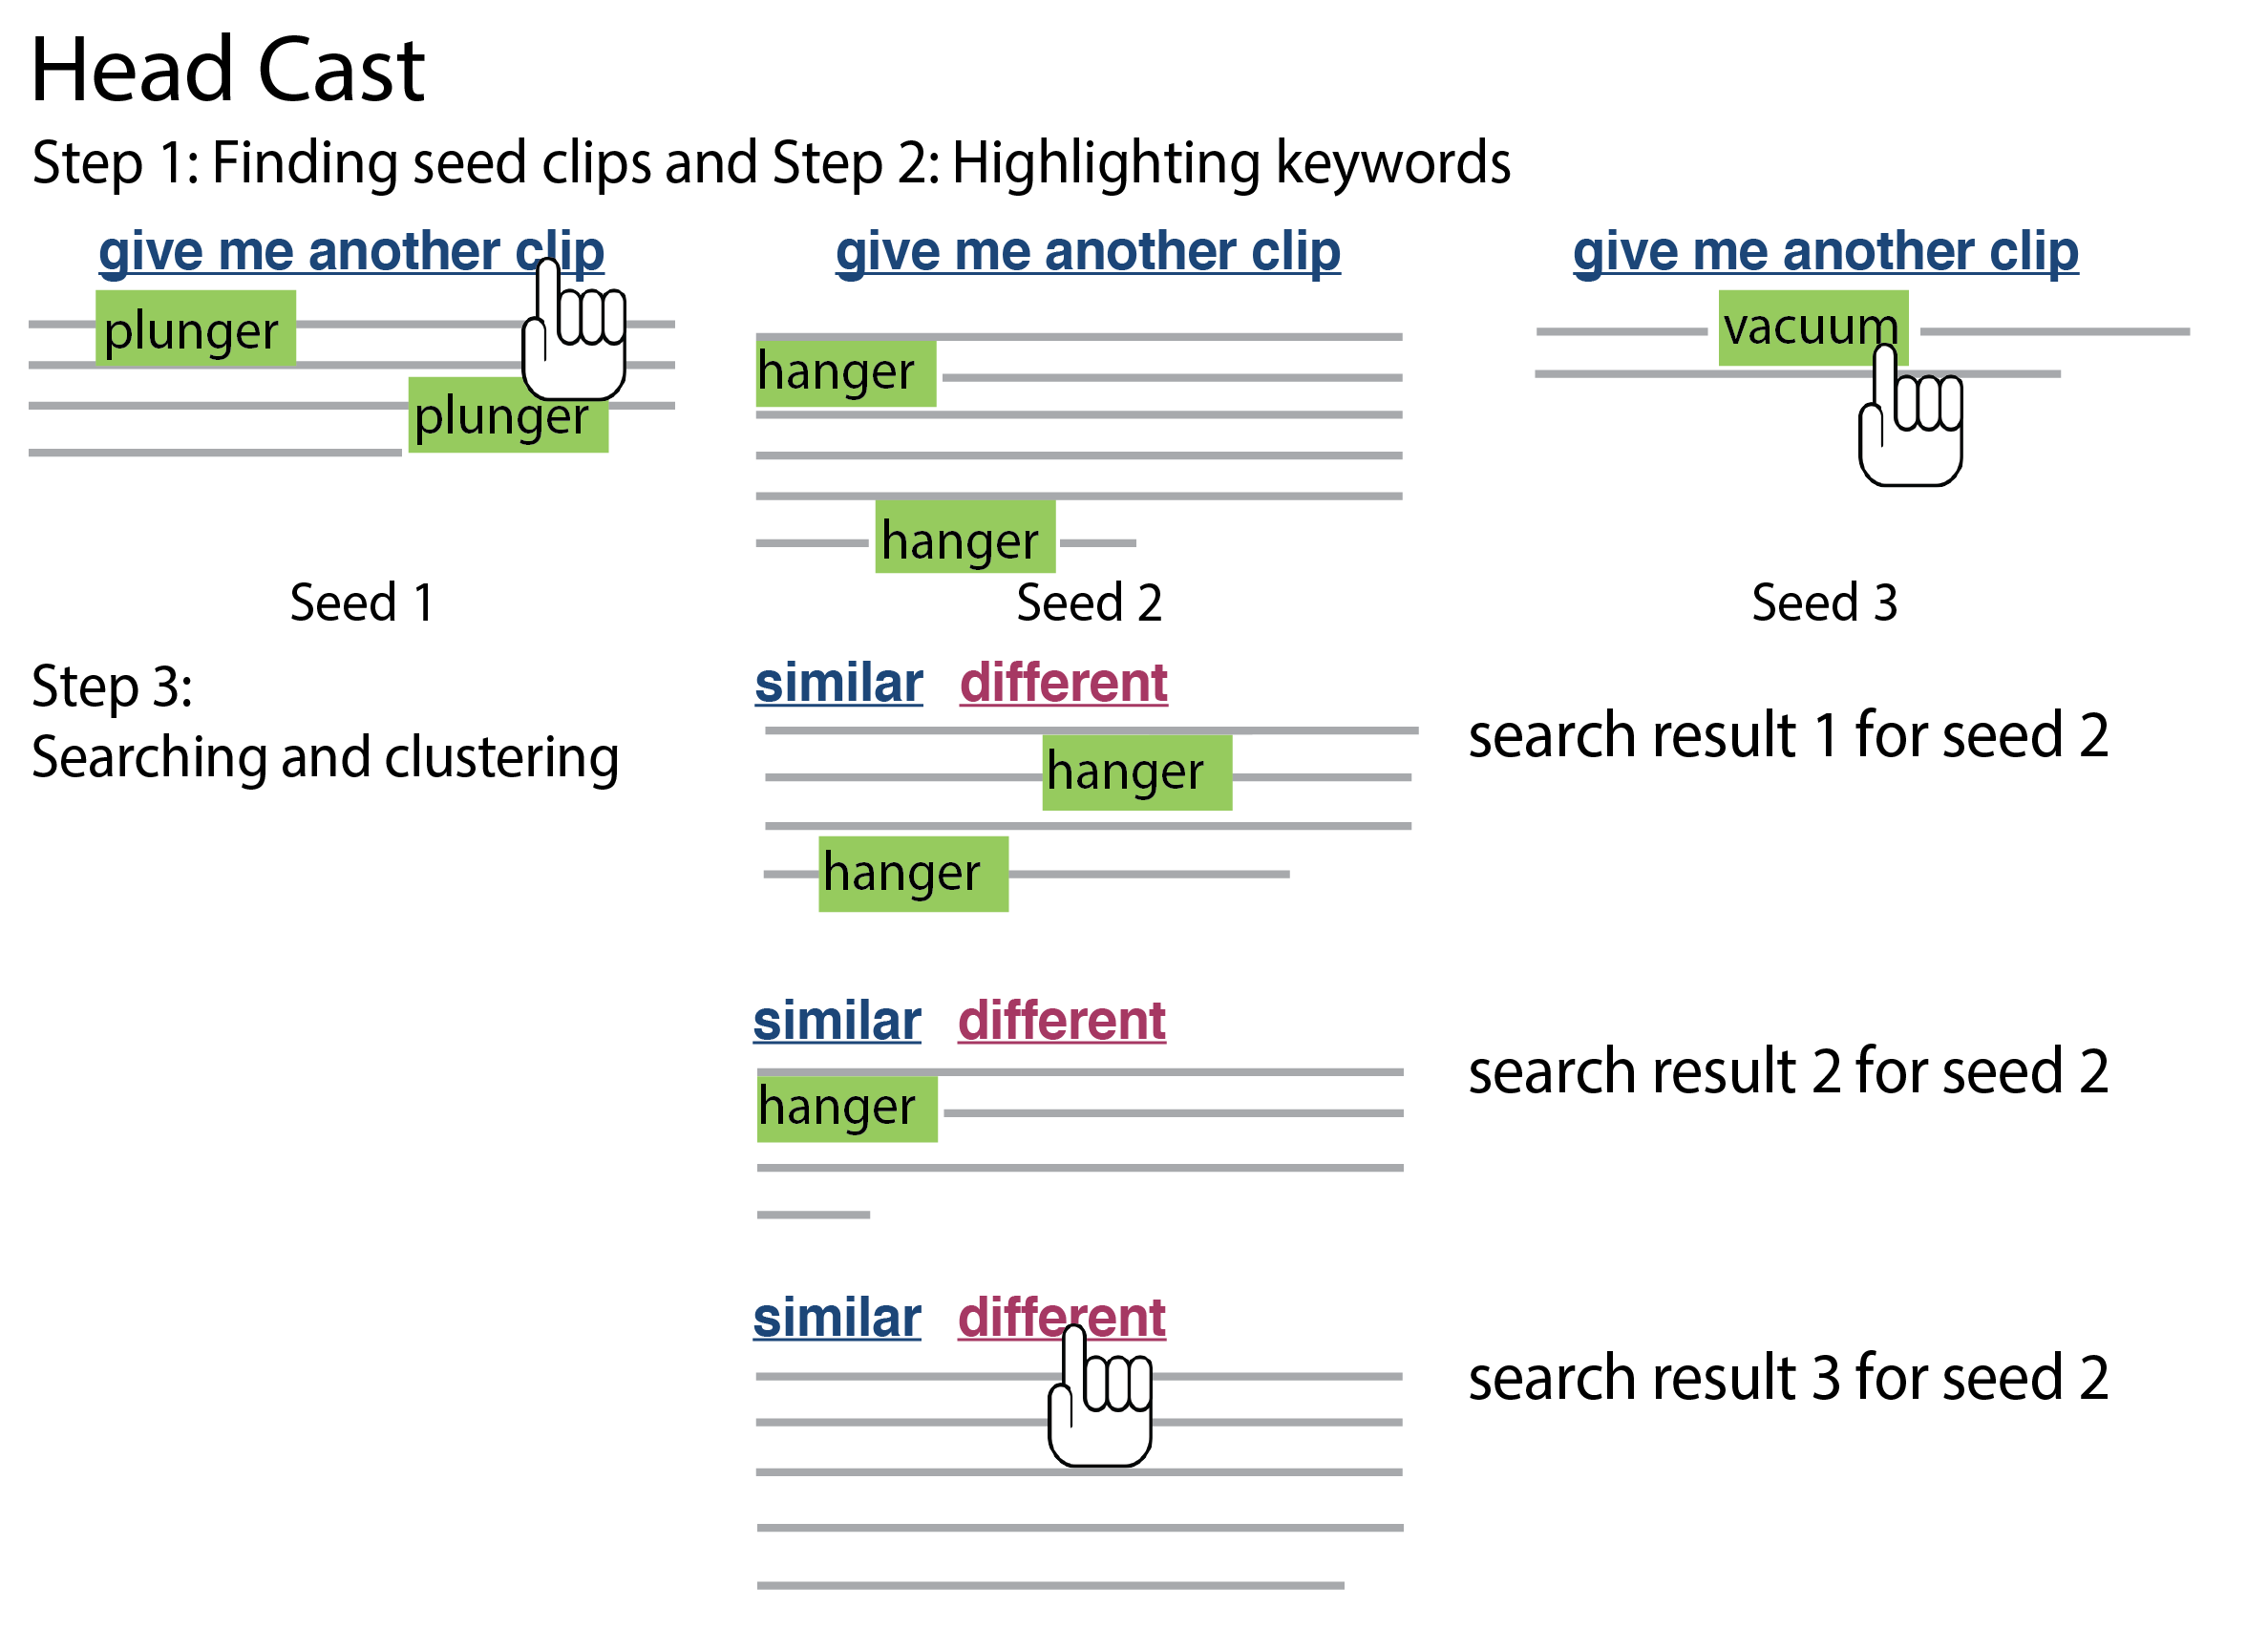
\includegraphics[width=0.6\columnwidth]{Chapters/Alloy/images/clusteringv2-04.png}
	\caption{The interface and steps of the Head Cast HIT.}
	\label{fig:phase1-hit}
\end{figure}

\subsection{The Head Cast}
The Head Cast aims to identify salient keywords to uncover the most common
categories in the head of the distribution. Doing so involves challenges in
providing workers sufficient context to know what a good category is, and also
in how to structure their work process in order to train a machine learning
algorithm to take over the classification of categories based on
human-identified seeds and keywords. 
Previous studies show that presenting multiple items from a collection can help
provide context to human workers \cite{medlin1978}, increasing the likelihood
of obtaining better clusters.  However, it can be difficult to determine how
much context is sufficient and how to produce a good sample that captures the
distribution of information of the whole dataset. 
Therefore, we introduce a new crowd-pattern we call ``\emph{sample and
    search}'' for providing global context through active sampling and
searching with keywords.   We ask crowdworkers to identify coherent categories
by presenting with four random items, but allowing them to replace each item by
random sampling from the entire dataset until they are confident that the items
will be in different categories in the final output.  This requirement gives them
the motivation to build up better global understanding of the dataset through
repeated sampling. After obtaining the four seed items, we ask crowdworkers to
identify keywords in each clips to search for related items in the dataset.
This process takes advantage of people's capacity of finding new information
\cite{pirolli1999information}. To create a familiar experience, we allow the
workers to freely change their query terms and update the search results in real
time. This way they can refine their searches based on the results, the same
way as when conducting online information foraging tasks \cite{jansen2009patterns}.
As shown in Figure~\ref{fig:phase1-hit}, the Head Cast HIT interface consists of three steps:

% The intuition is that a few keywords can be sufficient to
% identify important clusters in the head of the distribution
% \cite{huang2006text}. However, identifying important
% clusters and their salient words often requires a deep understanding of the
% data.

%The goal of Head Cast is to make use of human judgements to identify a set of
%keyword features and train an SVM model to partially cluster the given
%dataset \niki{this is a confusing way to introduce the SVM, since people will think you %are using it for clustering but you are using it more as a feature selection/similarity %metric enabler}.  Since it is infeasible to ask a crowdworker to organize the entire
%collection due to its size, each crowdworker
%worked on a small part of the dataset.  
% We implemented a three-stage workflow that uses machine learning models to augment initial human judgments.

%First, we use crowd workers to
%identify important topics and keywords through an interactive interface (Stage 1). Next we train an %SVM model to find the best set of features for predicting pairwise similarity of items based on the %human judgments (Stage
%2). Finally, we use those similarity judgments to create clusters using a
%hierarchical clustering backbone (Stage 3).

%\nathan{I changed the wording up here a bit}


% \jeffrz{***** If I were you, I'd make this two stages: stage 1 - human clustering, stage 2 - training and running an ML algorithm. this way you can echo the two-stage thing from the DESIGN section and reduce some redundancy}
% \joseph{two-phase actually refers to Head Cast and Tail Cast, not the steps here.}

% \subsubsection{Stage 1. Partial clustering and keyword extraction}

%Each crowdworker processes a
%portion of the input dataset using a set of four random seed clips we initially assign. 
%The idea is that most people are
%capable and familiar with picking out good keywords for retrieving documents
%through search. \nathan{maybe cite an IR paper about successful keyword search}.
%By asking crowdworkers to identify keywords in a seed clip to
%search for other clips that should be in the same category, we can record the
%process and gather not only clustering labels but also good feature dimensions
%at the same time.


\begin{enumerate}
    \setlength\itemsep{-1mm}

	\item \textbf{Finding seeds}:
    	Four random seed clips are presented to each crowdworker. Over each clip,
    	there is a button that allows them to replace the clip with another
    	random clip from the dataset.
		They are then asked to replace any clips
		that are too similar to the other seed clips.
		The workers repeatedly replace the seed clips
		until the four clips at hand belong to four different
		answer categories.
	\item \textbf{Highlighting keywords}:
	    The crowdworker is then instructed to highlight one to three
		unique keywords from each of the four seed clips that best identify
		their topics.  
	\item \textbf{Search and label}:
	    For each seed clip, we automatically search for
		similar clips from the entire corpus based on the highlighted keywords 
        and TF-IDF cosine similarity.
        The crowdworker is
		asked to label the top nine search results as \emph{similar} to or
		\emph{different} from their seed clips.
\end{enumerate}

% \niki{you need a rationale here; walk the reader through what problems you are solving with these steps so they can appreciate your solution.  Maybe reprupose stuff from the KA paper here, but you should adapt it so we don't get accused of plagiarism or something}

In Step 1, the crowdworkers need some understanding of the global context before
they can confidently judge that the seeds belong to different categories
in the final output. Previous work usually address this problem by presenting multiple
items to each crowdworker, in hopes of sampling both similar and dissimilar items
to give some sense of the global context. In reality it could be difficult to
judge how many items is sufficient for different datasets, and overly small size could lead to
bad samples that are unrepresentative of the global distribution.
We took a different approach by presenting fewer items at first,
but allowing workers to replace the seeds with random clips from
the dataset. This provide them both the mechanism and motivation to explore the dataset
until they have enough context to find good seed clips.

%The output of this stage is a number of potentially overlapping clusters, each
%contain one seed clip and nine other clips labeled as ``similar'' or
%``different''.

% unclear
%\begin{figure}[!h]
%	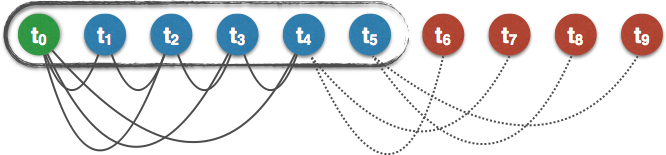
\includegraphics[width=0.9\columnwidth]{images/svm-clusters.png}
%	\caption{In Head Cast Stage1, crowdworkers create a cluster by selecting a
%		seed clip (green), and labeling 9 other clips as similar (blue) or
%		different (red). Each line connecting two clips indicates a training
%		events for Stage2.}
%	\label{fig:svm-clusters}
%\end{figure}

The intuition behind Step 2 is that people are already familiar with picking out good 
keywords for searching documents related to a concept via their online information
seeking experiences. In addition, requiring them to highlight unique keywords in the seeds
first, further ensures that they are familiar with the concepts in the seed clips, before
they search for similar items. In Step 3, the crowdworkers can still change and refine their
highlights from Step 2, and the system will refresh the search results in realtime. This
gives the crowdworkers both the motivation and mechanism to extract better keywords that lead
to better search results to label.
In Figure~\ref{fig:phase1-example}, we show two example clips from the datasets
collected using the two questions: \emph{How do I get my tomato plants to produce
more tomatoes?} and \emph{What does a planet need to support life?}
The highlighted words in each clips are the keywords selected by
one of the crowdworkers, showing that workers are finding useful words for classification.

%\niki{add rationale here about how this helps them in the next stage. you don't have to CALL it a design pattern since that's in KA, but give the intuition}

\begin{figure}
	\fbox{ \vbox{

		\ttfamily
        \scriptsize

% bad example
%		We had that problem too.  We snaked the bathroom tub, sink, \& stool so
%		many times.  The answer came to us when we had to replace the stool.
%		We found a \hilight{plumber} in the \hilight{yellow} \hilight{pages}.
%		Got some good recommendations.  They came and snaked the stack!  You
%		have to go on the roof for that.  If you can access the stack, rent as
%		big a plumber's snake as possible and to the job yourself.  Be sure to
%		ask the rental agency lots of questions, they want their equipment back
%		in good shape too. Be sure to clean the snaket (sic) off too.  That is
%		just plain common courtesy.  You will save lots of little tub snaking
%		jobs in the future
%
%		\rule{\columnwidth}{0.4pt}

		Tomato seedlings will need either strong, direct \hilight{sunlight} or
		14-18 hours under grow \hilight{lights}. Place the young plants only a
		couple of inches from florescent grow lights. Plant your tomatoes
		outside in the sunniest part of your vegetable plot.

		\rule{\columnwidth}{0.4pt}

        In its astrobiology roadmap, NASA has defined the principal
        habitability criteria as "extended regions of \hilight{liquid}
        \hilight{water}, conditions favourable for the assembly of complex
        organic molecules, and energy sources to sustain metabolism
	}}
	\caption{Example clips from two datasets with crowd keywords.}
	\label{fig:phase1-example}
\end{figure}


% \begin{figure}
% \footnotesize
% \hrule
% \vspace{2 pt}
% \textbf{Input:}\\
% \indent \ \ \ \ \ \ \ $S_{i,j}$: \ Sets of similar and different clips from Head Cast Stage 1\\
% \indent \ \ \ \ \ \ \ $K$: The set of all keywords from Head Cast Stage 1 \\
% \textbf{Output:} \\
% \indent \ \ \ \ \ \ \ \textit{Clusters}: Clusters of similar clips \\
% \indent \ \ \ \ \ \ \ \textit{Singletons}: Unclustered clips \\
% \textbf{Description:}
% \begin{algorithmic}[1]
% \STATE Let \textit{Sim} = \{$(t, t')$ $t, t' \in S_{i,j}$, $t, t'$ labaled "Similar"\}
% \STATE Let \textit{Diff} = \{$(t, t')$ $t$ labaled "Similar", $t'$ labaled "Different"\}
% \STATE \textbf{For} each $event_i \in$ \textit{Sim} $\cup$ \textit{Diff}:
%     \STATE \ \ \ \ \ \ Let $label_i$ = \textit{yes}, if $event_i \in$ \textit{Sim}, \textit{no} otherwise \\
%     \STATE \ \ \ \ \ \ Generate feature $feat_{i}$ based on $t, t', K$
% \STATE Train classifier \textit{M} using $label$, and $feat$
% \STATE \textit{Clusters}, \textit{Singletons} = HierchicalCluster($D$, $M$)
% \STATE \textbf{Return} \textit{Clusters}, \textit{Singletons}
% \end{algorithmic}
% \hrule
% \label{fig:phaseAstage2stage3}
% \caption{Pseudocode for Head Cast: Stages 2 and 3}
% \end{figure}

%\subsubsection{Stage 2. Similarity function: training an SVM model}

To learn a similarity function between clips, we use the crowd
labels and keywords to train a classifier that predict how likely two clips
to be labeled as similar.
Although the judgments from workers via the HIT interface about which clips go together provide valuable training information, we need to leverage these judgments to bootstrap similarity judgments for the clips that they did not label and to resolve potentially conflicting or partial category judgments. 
To do so we trained an SVM classifier in real-time to identify the set of keywords that are most indicative of categories and predict whether two clips in the dataset belonged to the same cluster.  
The training events
are all possible pairwise combinations of clips in the clusters obtained with the HIT interface,
which may include both positive (similar) and negative (different).
The feature dimensions are all the keywords highlighted by the
crowdworkers, and the value of each dimension is the product of
the number of times that keyword occurred in the two clips.
In general,  the keywords labeled by the crowdworkers contain little irrelevant information
compared to all words in the clips, but there could
still be some highlighted words that are not indicative of a category. For
example, one crowdworker worked on the dataset for ``\emph{How do I unclog my
	bathtub drain?}'' labeled ``\emph{use}'', ``\emph{a}'', and ``\emph{plunger}'' as
three keywords. Even though \emph{plunger} is a very
indicative feature for clustering this dataset, the first two highlighted words
seem too general to be useful. 
Using a linear kernel to
estimate the weights for the different dimensions (i.e., keywords) seems well suited for
our purpose \cite{chang2011libsvm, wu2004probability}.
Further, if the same keyword is used by different crowdworkers but lead to
very different labels, the linear SVM model will give lower weight to the corresponding dimention and
thus lower the effects of keywords that are less indicative of the categories.
We use LIBSVM which
implements a variant of Platt scaling to estimate probability 
\cite{lin2007note,platt1999probabilistic}. The overall intuition is that the SVM classifier is doing a form of feature selection, weighting those words in clips that could maximally distinguish clips amongst clusters. 
% \niki{I don't know if this is right, but you need to provide something like this as a rationale for each of your sections. Usually good to start with a problem you are trying to solve.}





% \jeffrz{do you need the rest of the stuff here? sounds too technical unless related work is important or reviewers complained last time}
% \joseph{this is from the reviewers last time (why is SVM needed / selected), i am shortening it by taking out the part with selecting bigram and trigrams.}
%This can potentially be solved by allowing turkers to extract
%bi-gram or tri-gram features from the clips, but it will also %increase interface
%complexity and decrease the coverage of the identified features %(e.g.,
%\emph{plunger} vs \emph{use a plunger}). On the other hand, a linear


In a preliminary experiment, we tested using all words in the clips as features to train
the SVM model. The intuition is machine algorithms might do a better job at identifying
keywords that can outperform keywords identified by crowdworkers. However, the results
show that using all words as features did not yield better results, and having much
higher feature dimensions increases the training time significantly.

%\subsubsection{Stage 3. Hierarchical clustering}
%\niki{is this actually the Gather stage? maybe integrate it into the bottom of the gather backbone section below?}

Finally, with the probability output of the SVM model 
as a similarity function between clips and a stopping threshold of $0.5$ probability,
we use a hierarchical clustering algorithm 
that serves as the Gather Backbone to capture head clusters. 

% We also tested different thresholds and found that 0.5 is the best performing condition overall. The output is a set of clustered and
% unclustered clips.

%\jeffrz{I have no idea what BACKBONE: HIERARCHICAL CLUSTERING means. make it more descriptive. (though I'd watch a movie titled that)}


\begin{figure}
	\centering
	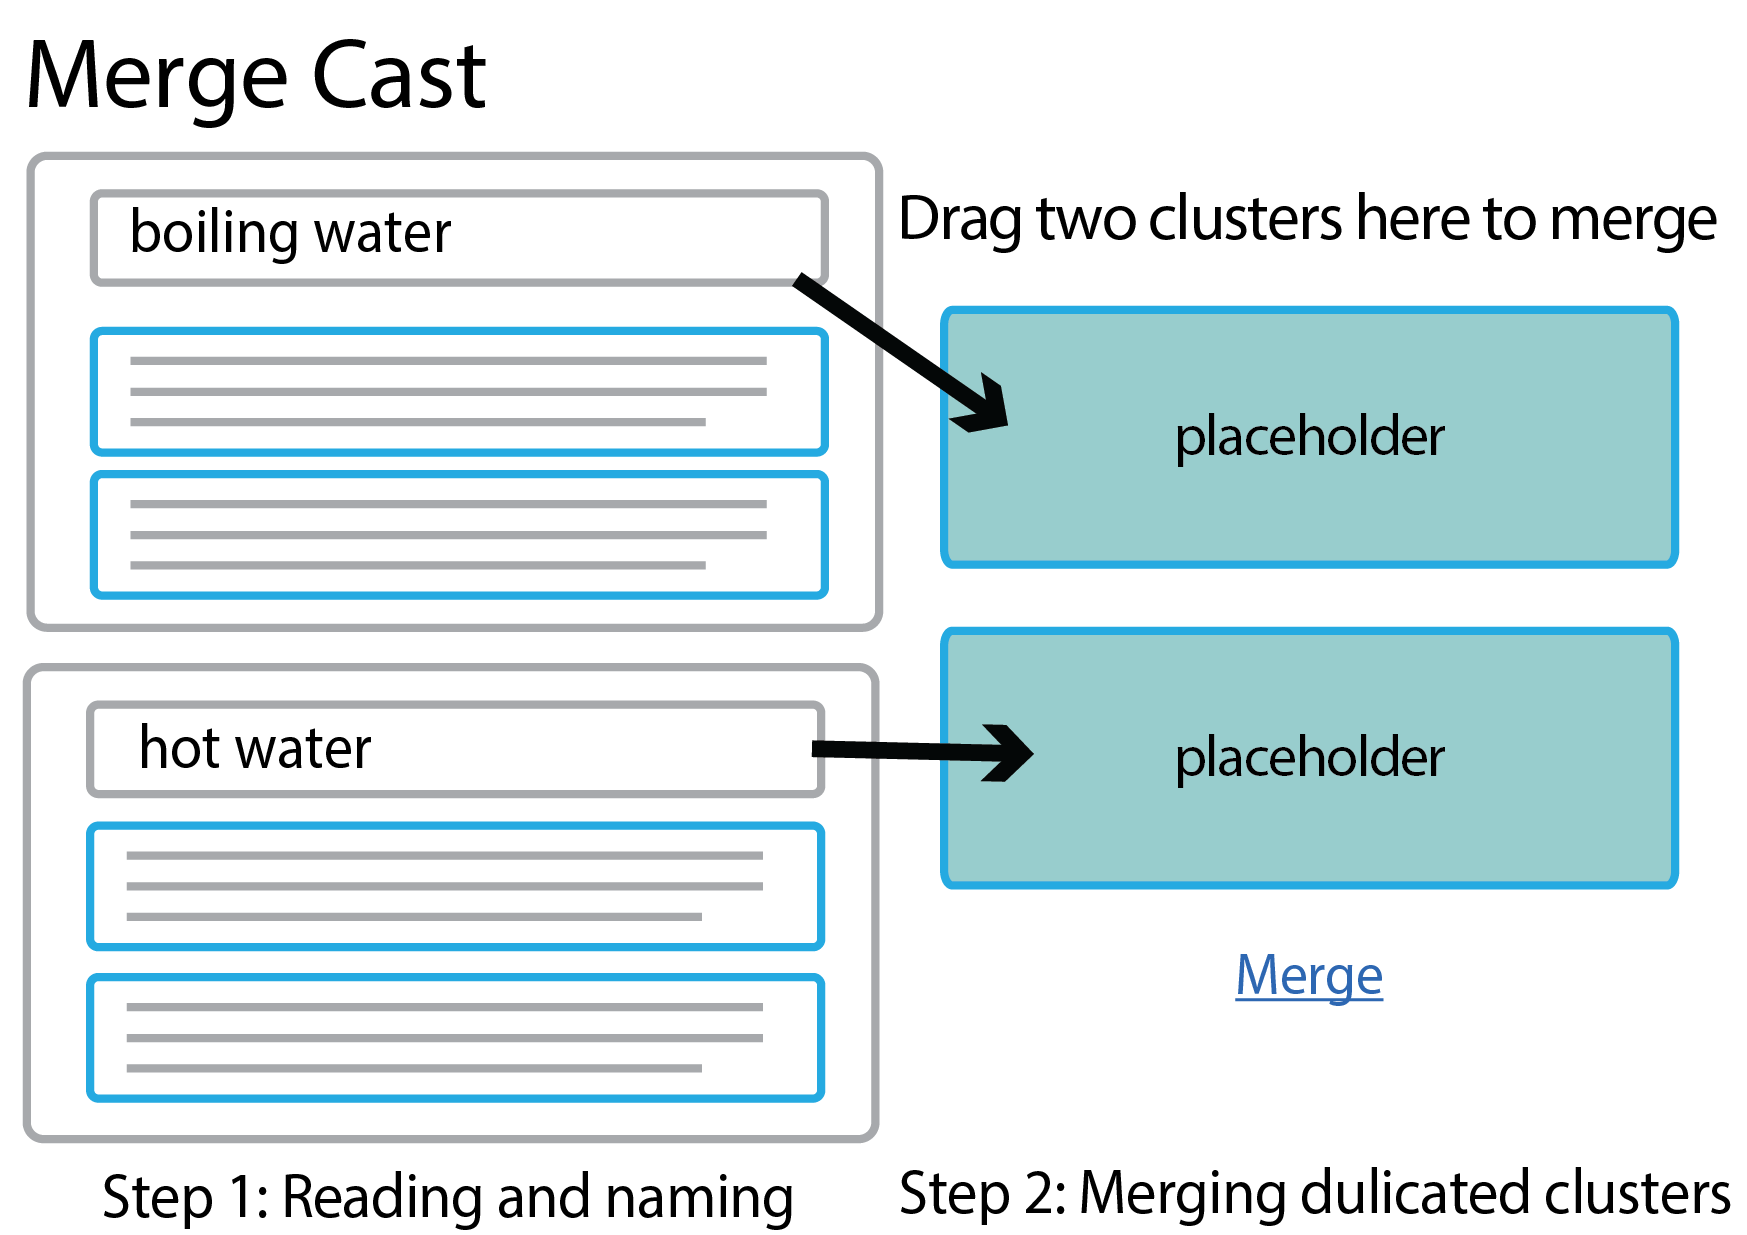
\includegraphics[width=0.47\columnwidth]{Chapters/Alloy/images/clusteringv2-02.png}
	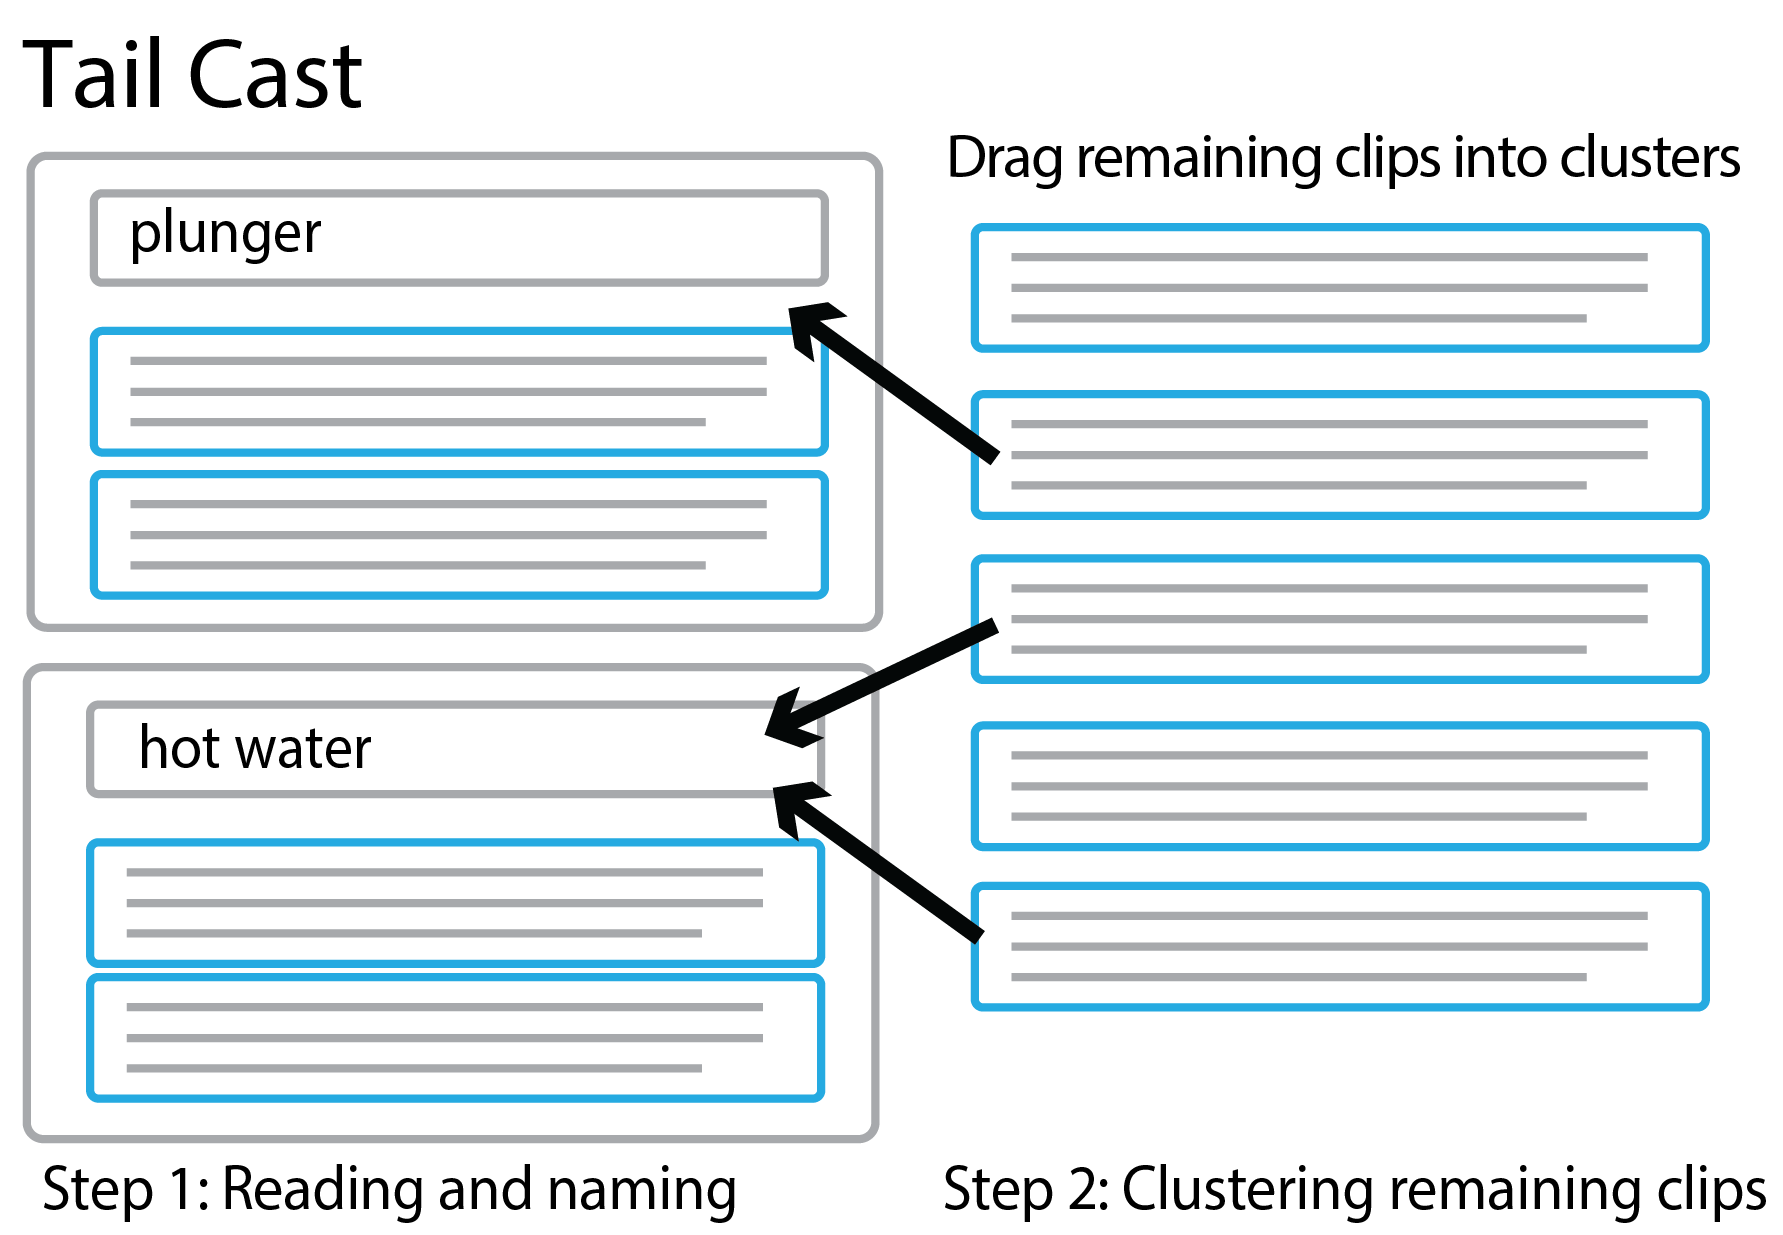
\includegraphics[width=0.47\columnwidth]{Chapters/Alloy/images/clusteringv2-03.png}
	\caption[HIT interface for the Merge Cast and the Tail Cast.]
        {The HITs for Merge Cast: Naming and merging existing
		clusters and Tail Cast: Clustering remaining clips.}
	\label{fig:phase2-hit}
\end{figure}

\subsection{Gather Backbone: Hierarchical Clustering}

\label{sec:hclustering}

%\jeffrz{I have no idea what primitives are now, and I am really, really lost. rewrite the two paragraphs as one}

Using a multiple-stage approach with different types of microtasks can make it
difficult to fuse together the different crowd judgements to form a coherent
result.  A key element to our approach in \textit{casting} for category
judgments in different ways is that we have a unifying mechanism to
\textit{gather} them back together.  For example, throughout our process we
cast for human category judgments in very different ways, including having
people identify seed clusters (the Head Cast), merge duplicated categories (the
Merge Cast), and classify the tail of the distribution (the Tail Cast).
Instead of creating ad-hoc links between these judgments we propose using a
unifying gathering mechanism composed of a machine learning backbone
which translates the different
\textit{casted} judgments into similarity strengths used as the basis of
clustering. We believe this \textit{Cast and Gather} pattern may be useful as
a way to conceptualize the relationship between machine algorithms and crowd
judgments for a variety of tasks.

% The Casts are designed to capture the varying types of human
% judgements that can be used to cluster different portions of the dataset. At
% different phases, the workflow iteratively creates new categories that cover
% more items in the dataset.

% remove candidate
To build a complete clustering workflow with multiple casts, we use a
hierarchical clustering algorithm as the backbone that connects different
casts. More specifically, the backbone algorithm  fuses the judgements
from different crowdworkers working on the same cast into
clusters, which, in turn, become the
shared context transferred to the next cast of the workflow.

With a clip similarity function from the prior cast and a stopping threshold, 
the hierarchical clustering method initially treats each clip as a
cluster by itself, and iteratively merges the two most similar clusters until a
threshold is reached. The result is a partially clustered dataset
with clusters and singletons. 
When the backbone is used after the last cast in the workflow, each
singleton is then merged into the most similar cluster.
The similarity between two clusters is defined as:

\vspace{-2mm}
\begin{equation}
	ClusterSim(\omega_1, \omega_2) = \frac{1}{|\omega_1||\omega_2|} \sum_{t_j \in \omega_1} \sum_{t_k \in \omega_2} ClipSim(t_j, t_k)
\end{equation}
\vspace{-1mm}

where $\omega_1$ and $\omega_2$ are the two clusters, $t_j$ and $t_k$ are each of the
clips in $\omega_1$ and $\omega_2$, respectively, and the $ClipSim()$ function is
the given similarity function between clips.


%\jeffrz{So we have Phase A, Consolidation Phase, and Phase B? I'm lost. Pick a "Phase" nomenclature and stick to it. I wouldn't do "Phase A", I'd give it a descriptive name kind of like you do here}
\subsection{The Merge Cast}
%\jeffrz{tighten this up. can you get by without "stages" and just paragraphs? you're losing lots of space on subheadings and nomenclature that may not be helpful unless it pops up again a few times in the paper}
%\niki{I would consistently go with "The Head Cast" instead of "Head Cast"}
While the Head Cast is designed to find the large clusters in the head of the
distribution, since each crowdworker works independently,
some of those clusters may actually
be different subsets of the same larger category or the same categories based
on different keywords (e.g., \emph{sunlight} vs \emph{natural lighting}).  The Merge Cast is designed to consolidate 
existing clusters by merging duplicated categories.  The input to this
cast is a set of clusters that may or may not cover the entire dataset,
and the output is fewer or equal number of clusters each with a list of ranked
short descriptions. 
The
challenge with detecting duplicate categories is that people need to understand
what is in each category first. 
We start by presenting a set of existing clusters, and asking crowdworkers to name 
each of them. This acts as a defensive design\cite{kittur2008crowdsourcing} that
ensures the crowdworkers
understand the current context (scope and abstraction level), and also to obtain
short descriptions for each of the clusters. 
Crowdworkers are
then asked to merge identical categories by dragging them into the
placeholders on the right (Figure~\ref{fig:phase2-hit}).

If there are too many head clusters to fit into a microtask,
the Merge Cast can be run recursively by
first running on disjoint sets of existing
clusters to consolidate them independently. Then, run another sets of
Merge Cast on the output of each initial Merge Casts, and recurse until
the output reduces to a set of clusters that
could be presented in a global Merge Cast to ensure consistency. 
The assumption here is that the set of clusters in the final output of Alloy should be
manageable by a single person to be useful.
We also wanted to point out that the number of clusters is likely to scale much slower than
the size of the dataset for many real-world data.
% In all six datasets we have tested, with up to 160 items, we have not encounter a case where we needed to run Merge Cast recursively.

% We can more formally characterize the scaling function as $T = log_c~N$,
% where $c$ represents the sparseness parameter of a dataset, $N$ the number of items 
% in the dataset, and $T$ the number of categories. The upper-bound limitation of 
% Alloy is then $T < L$, where $L$ is a limit on the complexity of a task given the characteristics of the 
% human computation platform utilized. Intuitively, this means that the Merge Cast will scale better 
% when the dataset involves fewer categories that explain more of the data, and when the human computation 
% platform supports more complex tasks.



With the labels from the crowdworkers,
we will again use the Gather Backbone to combine the judgements. The goal
is to merge existing clusters if more than half of the crowdworkers also
merged them in their solutions. Since in the Merge Cast
workers can not break up existing clusters or reassign clips, we can formulate 
the clip similarity function as:

\vspace{-2mm}
\begin{equation}
	ClipSim(t_1, t_2) = \frac{1}{N} |\{\omega: t_1, t_2 \in \omega \; and \; \omega \in \Omega\}|
\end{equation}
\vspace{-1mm}



where $t_1, t_2$ are the two clips, $N$ is the total number of crowdworkers,
$\Omega$ is the set of all clusters created by all crowdworkers, and $\omega$ is any cluster that contains both clips. This
function is robust against a few workers doing a
poor job. For example, if one crowdworker assigned every clip in the dataset to
a single, general cluster (e.g., \emph{answers}), the effect to the similarity function
would be equivalent to having one less crowdworker and applying Laplacian smoothing.
It is a common concern for crowd-based clustering methods
that novice workers may create overly abstract categories (e.g., \emph{solutions} or
\emph{tips}), that covers
all items in the datasets.
With our approach,
it would require more than half of the workers to merge all items into a single cluster
to generate a single cluster in the output.

% redundant
% We use the similarity function with a threshold of 0.5 to perform hierarchical
% clustering as described in the previous subsection, which is the equivalent of
% merging existing clusters when more than half of the crowdworkers also merged
% them in their solutions.

% \subsubsection{Stage 3. Ranking Cluster Names}

From the output of the Gather Backbone, we rank the short descriptions
associated with each cluster.
Since clips are labeled by multiple crowdworkers, each cluster
is associated with multiple
descriptions via its clips. We use the F1 metric to rank these names to
find the most representative description for each cluster, where the precision
of a name label is defined as
the number of clips in the cluster that it associates with divided by the size of the cluster,
and recall as divided by the total number of clips associated with it.

\subsection{The Tail Cast}

The Tail Cast is designed to clean up the remaining singleton clips by classifying
them into existing clusters or creating new clusters.  The intuition is that
even though machine learning techniques can produce high performance output,
sometimes it is achieved at the expense of sacrificing the border cases.
Human-guided ``clean up'' is often necessary for data produced by a machine
learning model.  The input of this cast is a set of existing clusters
(with or without short descriptions) and a set of remaining clips. The
output is a set of clusters with short descriptions.

We use an interface similar to the Merge Cast (Figure~\ref{fig:phase2-hit}),
and asked crowdworkers to review or name each of the existing clusters first,
so that they build up better global understanding of the dataset before they
organize the remaining clips. If Merge Cast was performed previously, their
names are presented to lower cognitive load.  The crowdworkers are then
instructed to cluster the unorganized clips shown on the right by assigning
them into existing clusters, creating new clusters, or removing uninformative
clips.  If there are too many remaining clips to fit into a single microtask,
they are partitioned into groups of 20 items.  Even though we may be dividing
the remaining clips into partitions, all workers in the Tail Cast starts with
learning the same global context that is the set of existing clusters from the
Head Cast.

%\subsubsection{Stage 1. Clustering with global constraint}

%\jeffrz{this is an example where the nomenclature gets to be a problem - I'm confused when you say "Phase B HIT". is it to make it different from a Phase A HIT? Why not give them more descriptive terms.}

% \subsubsection{Distributed Tail Cast}

% The amount of work in the Tail Cast is determined by both the size of the
% corpus and amount of clips covered by the Head Cast clusters.  It might not scale
% well if the size of the dataset increases.  For example, for a dataset of
% 200 clips, even if the Head Cast clusters cover 75\% of the items, the
% remaining 50 clips are still too many for a single crowdworker to organize in
% one HIT.
% Therefore, for datasets with more than 100 items, instead of showing all
% remaining clips to a single crowdworker, we distribute them across
% different HITs to different crowdworkers so that each crowdworker only work on
% 20 items. The idea is that even though they only see a small portion of the dataset,
% they are still organizing them based on the same existing context that is the
% Head Cast clusters.

%\subsubsection{Stage 2. Integrate clusters from multiple crowdworkers}
%\niki{aren't these just the Gather and then Merge Cast? rename if so?}

Finally, we use the Backbone Gather again to combine the multiple solutions
from the crowdworkers. The goal is analogous to the goal of the Merge Cast: if
two clips are assigned to the same category by more than half of the
crowdworkers, they should be in the same cluster in the combined solution.
For the similarity function, we simply replace the
variable $N$ in Equation~2 by the degree of redundancy.

% \begin{equation}
% 	\begin{split}
% 	ClipSim(t_1, t_2) & = \frac{1}{R} |\{\omega_j \forall t_1, t_2 \in \omega_j \; and \; \omega_j \in \Omega\}| \\
% 	                R & = \frac{20 * N}{|T|}
% 	\end{split}
% \end{equation}
% 
% where the redundancy $R$ is defined as number of HITs posted $N$, times the
% number of clips in each HIT $20$, divided by the number of remaining clips from
% Head Cast $|T|$.

% Finally, we can extract short descriptions for each cluster using the same
% F1 ranking described in the Merge Cast section.

% 
% \subsection{Time Complexity}

% \joseph{new}
% For each cast, we post different numbers of redundant HITs to Amazon Mechanical
% Turk. We can measure the time complexity by number of HITs posted in parallel.
% The time complexity for the Head Cast and the Merge Cast are $O(r_h)$ and
% $O(r_m)$ respectively, where $r_h$ and $r_m$ are the amount of redundancy.
% For the Tail Cast, the time complexity
% is $O(r_t  \lceil n / t \rceil)$, where $r_t$ is the amount of redundancy, $n$
% is the number of remaining items, and $t$ is the number of items presented to
% each crowdworker. In the Experiment Section, we will show the results of using
% different $r_h$ and $r_t$ on the same datasets to test the robustness of Alloy.





% \section{Core Design Patterns}
% %!TEX root = main.tex

% In this section, we discuss the reasoning behind the design of the proposed method.
% We will present the design patterns utilized in three HIT
% interfaces, and how these designs help in producing better clustering results.

\joseph{new}
In addition to the system itself, we identified two higher level design patterns
that could be useful for future crowd-driven information systems.
% First, a Two Stage approach that uses
% machine algorithms for scale and employs the crowd for quality.
% Second, a Cast and Gather framework that connects multiple stages for incremental improvements.
% Finally, a Request for Context
% pattern that allows crowdworkers to freely explore the corpus for context.

% 
% \subsection{Two Stage Clustering}
% A key difference from previous work on crowd clustering is our two-stage model
% of clustering. 
% %There is a conflict between providing sufficient context
% %for identifying categories in a skewed distribution and the limited context capacity of 
% %microtasks that are suitable for posting to online crowdsourcing marketplaces such as Amazon Mechanical Turk. Further, i
% It is common for a collection of information to be not evenly distributed across topics but instead
% follow a highly skewed distribution \cite{white2007studying}.
% In such cases the head of the topic distribution
% contains a disproportionate number of clips, and once a human has labeled a few
% of these clips it is inefficient to continue using human labor to finish
% labeling them as automated methods can do a reasonably good job.  Conversely,
% the tail of the topic distribution contains topics with few clips,
% and expending resources to train a machine learning algorithm to
% identify these sparse topics is less advantageous, while it is comparatively
% easy for humans to classify these clips.  

% Previous crowdsourcing research has shown success in using the crowds to capture uncommon cases in a long tailed distribution to improve inline answers in Web search engines \cite{Bernstein:2012:DAS:2207676.2207710}. We extend this approach further so that
% humans can also classify the clips for which the machine classifier has low
% confidence. 


\subsection{Sample and Search}
Previous studies show that presenting multiple items from a collection can help
provide context to human workers \cite{medlin1978}, increasing the likelihood
of obtaining better clusters.  However, it can be difficult to determine how
much context is sufficient and how to produce a good sample that captures the distribution of information in the larger dataset. 
%For example, if the sample size is too small, and
%the presented items are too similar, the workers may group all items into a
%very general class (e.g., \emph{tips}), or overly specific classes.
In one instance of previous work up to 10 items were presented to each
crowdworker to ensure a better chance of sampling both
similar and dissimilar items from the dataset \cite{andre2014crowd}.
We take a different approach and ask crowdworkers to identify coherent categories by
presenting fewer items, but allowing them to replace each item by random sampling
from the entire dataset until they are confident that all items are in different
categories in the final output.
This process requires building some degree of global understanding of the
information space, and we give workers the freedom and motivation to explore the
dataset until they have enough context. After obtaining the seed items by repeated sampling,
we ask crowdworkers to identify keywords in each clips to search for related items in the dataset.
This process takes advantage of people's ability to find new information \cite{pirolli1999information}. To create a familiar experience, we allow the workers to freely change their query terms and show the search results in real time. This way they can refine their searches just as when conducting online information foraging (cite query reformulation), and we also have better chance of obtaining better keywords and clusters.



\subsection{Cast and Gather}
Using a multiple-stage approach with different types of microtasks
can make it difficult to fuse together the different crowd judgements to form
a coherent result.
A key element to our approach in \textit{casting} for category judgments in
different ways is that we have a unifying mechanism to \textit{gather} them back
together.  For example, throughout our process we cast for human category
judgments in very different ways, including having people identify seeds,
classify items relative to those seeds, merge categories, identify categories
as trash, create new categories, and classify the tail of the distribution.
Instead of creating ad-hoc links between these judgments we propose
using a unifying gathering mechanism composed of a machine learning backbone
(in our case, a hierarchical clustering algorithm) which translates the
different \textit{casted} judgments into similarity strengths used as the basis of
clustering.   We believe this \textit{Cast and Gather} pattern may be useful as a
way to conceptualize the relationship between machine algorithms and crowd
judgments for a variety of tasks. While the algorithm used as the unifying
backbone may differ across task needs, the important core features of the hierarchical
clustering algorithm we used include: 1) it can
be done iteratively, so that many worker judgments in many different stages
could be repeatedly fed into the same algorithm; 2) it uses a global similarity
space, so that different judgments can all be mapped into similarity scores;
and 3) it is distributed, such that scores between pairs of items can be
updated independently of other items.


%\subsection{Global Context through Self-selected Sampling}
%\niki{I don't really understand this paragraph. maybe move this and the next
%    section to method? this fits in with the finding seeds part and the next
%    section with keyword part.}
%Previous studies show that presenting multiple items from a collection can
%help provide context to human workers \cite{medlin1978},
%increasing the likelihood of obtaining better clusters.  However, it can be
%difficult to select such items. On one hand, if the presented items are too
%similar, the workers may group all items into one big cluster using a very
%general and abstract class, e.g., \emph{answers} or \emph{tips}.
%Alternatively, they may also create multiple clusters that effectively divide
%the items presented, but they may be too fine-grained in the global context. On
%the other hand, if the presented items are very different from each other
%(e.g., one item from each desired class) the workers may not be able to
%recognize the salient features that help to determine cluster membership, due
%to the limited number of examples for each abstract class.
%
%In one instance of previous work up to 10 items were presented to each
%crowdworker \cite{andre2014crowd}, to ensure a better chance of sampling both
%similar and dissimilar items from the dataset. The amount of data presented can
%be overwhelming at times, especially if the items are not easily understood at
%a glance. Further, it can also be ineffective if the datasets contain
%many abstract classes. In the first Phase of our proposed method,
%we take a different approach by presenting
%the workers with fewer items from the dataset, but allowing them to replace
%each item with a clip randomly sampled from the dataset. The instructions of
%this exploratory process is to find a few items each from a different
%conceptual class, which requires some degree of global understanding of the
%dataset.  This way, the workers have the freedom and motivation to explore the
%dataset, and build up their mental model of the information-scape in the
%progress. The process stops when the crowdworker feels that they have sufficient
%global knowledge to judge the seed items at hand as belonging to different clusters in the
%final output. Overall, this design aligns nicely with the goal of the proposed
%method.
%
%\subsection{Keyword Sampling and Feedback}
%
%To find other clips similar to the seed clips by human judgements, we
%built on an intuition
%developed by manually clustering clips ourselves, in which we found that we frequently
%categorized clips based on a small number of keywords.  However, finding those
%keywords is itself a challenge for automated methods, as the same scarcity
%problems come into play. Instead, we developed a sampling and feedback method
%for crowdworkers to identify good keywords, in which they simply clicked on a
%keyword to select it and immediately saw feedback in terms of the most related
%clips identified by the machine.  They could then refine their keywords to
%improve the relevancy of the returned clips. This helped crowdworkers be more
%efficient about identifying relevant clips, and also served to gather the most
%salient features for training a similarity model in the later stage.  
%\joseph{move to method?} Also, by
%having crowdworkers labeling clips with both positive and negative tags, we can
%gather both positive and negative examples for training. Further, by labeling
%items from search results, crowdworkers are labeling the edge cases for the
%negative examples (i.e., superficially similar but conceptual different clips).
%This also fits well with the idea behind SVMs, which rely on the edge cases to
%find a good decision boundary.
%\joseph{move the SVM part to method}
%



\begin{table}
  \centering
  \footnotesize

% question, number of sources, number of clips, number of turkers
  \begin{tabular}{ l r r r r r }
    \hline
	Dataset &
    sources &
    workers &
    clips &
	bad &
    clusters \\
    \hline
	% 102
	\textbf{Q1}:\emph{How do I unclog my bathtub drain?} & 7 & 16 & 75 & 25\% & 8 \\
  
	% 115	
	\textbf{Q2}:\emph{How do I get my tomato plants to produce more tomatoes?} & 18 & 13 & 100 & 10\% & 8 \\
 
	% 96
	\textbf{Q3}:\emph{What does a planet need to support life?} & 19 & 19 & 88 & 31\% & 7  \\

	% 116
	\textbf{Q4}:\emph{What are the best day trips possible from Barcelona, Spain?} & 12 & 12 & 90 & 18\% & 16  \\

	% 137
	\textbf{Q5}:\emph{How to reduce your carbon footprint?} & 20 & 11 & 160 & 14\% & 11 \\

	% ???
	\textbf{Q6}:\emph{How do I unclog my bathtub drain?} & 17 & 23 & 159 & 14\% & 11 \\
	
	\textbf{Wiki}: Talk page sections for the Wikipedia \emph{Hummus} article & N/A & N/A & 126 & 0\% & 13 \\ 
	
	\textbf{CSCW}: Abstract sections of CSCW 2015 accepted papers & N/A & N/A & 135 & 0\% & 45 \\ 
    \hline
  \end{tabular}
  \caption{Datasets used for evaluation}
  \label{tab:datasets}
\end{table}

\section{Evaluation}

\subsection{Evaluation Metric and Datasets}
%!TEX root = main.tex
% \niki{maybe the name of this section should be Evaluation instead of NMI}
Unlike evaluating a classification task, which would typically be based on
the precision and recall of pre-defined classes, evaluating clusters is not as
straightforward due to the potentially different number of classes in the gold-standard and 
the system output. For example, high precision can be achieved by simply having more
clusters in the output and the mapping between them.
To address this, we use the normalized mutual information metric (NMI), which is a symmetric measurement sensitive to both the
number of clusters, and the precision of each cluster.  Specifically, it
compares all possible cluster mappings to calculate the mutual information, and
normalizes by the mean entropy so that the numbers are comparable between different
datasets:

% divide it by the mean entropy of the two sets of clusters so that results
% across different datasets are comparable, and unbiased by the innate complexity
% of different questions.

% For example, the output of the system and the gold standard
% can have different number of clusters. They can either be many-to-one mappings
% (mapping multiple fine-grained clusters to a more abstract cluster), or
% clusters created based on different concepts. It is also not as informative to
% use precision and recall to evaluate clustering results. For example, the
% purity metric computes the average precision of all clusters in the system
% output, however, maximum purity can be easily achieved if each clip is its own
% cluster. Instead, we use the Normalized Mutual Information from Information
% Theory and Information Retrieval to evaluate the difference between system
% output and the gold-standard clusters \cite{manning2008introduction}.

\vspace{-3mm}
\begin{equation}
NMI(\Omega, C) = \frac{I(\Omega, C)}{0.5 * [H(\Omega) + H(C)]}
\end{equation}
\vspace{-2mm}

where $\Omega$ is the output clusters and $C$ is the gold-standard clusters.
The mutual information $I$ is defined as:


\vspace{-3mm}
\begin{equation}
	\begin{split}
I(\Omega, C) & = \sum_k \sum_j P(\omega_k \cap c_j) log \frac{P(\omega_k \cap c_j)}{P(\omega_k)P(c_j)} 
% \\
  %           & = \sum_k \sum_j \frac{|\omega_k \cap c_j|}{N} log \frac{N|\omega_k \cap c_j|}{|\omega_k||c_j|}
	 \end{split}
 \end{equation}
\vspace{-2mm}

where $\omega_k$ and $c_j$ denotes each of the clusters in $\Omega$ and $C$,
respectively. The probability $P(\omega)$ of item set $\omega$ is defined as
$|\omega|/N$, where N is the number of total items. Finally, the mutual
information is normalized by the mean entropy of $\Omega$ and $C$, so that the
scores are comparable across datasets.
To give some intuition, given $w$ that maps to a gold-standard
cluster $c$, we can calculate the precision by $P(w \cap c) / P(w)$ and recall
by $P(w \cap c)/P(c)$, and the metric considers both with $P(w \cap c)/P(w)P(c)$.
However, in reality it may be difficult to obtain such mappings, and the metric simply
sums up scores of all possible mappings weighted by probability $P(w \cap c)$.

We use NMI for it is widely found in the literature for clustering evaluation.
A more recent study found that it might favor datasets with more clusters, and
proposed a variant that adjusts for randomness (AMI,
\cite{vinh2009information}).  We acknowledge this is a potential limitation,
but found that the number of clusters Alloy produced were quite close to the
gold-standard (average 10.3 vs 10.2), suggesting the concerns may be minimized.
To be on the safe side, we also measured Alloy's performance using AMI on two
datasets and found similar results. 


% Finally, the entropy $H$ is defined as:

% \begin{equation}
% 	\begin{split}
% H(\Omega) & = - \sum_k P(\omega_k) log P(\omega_k) \\
%           & = - \sum_k \frac{|\omega_k|}{N} log \frac{|\omega_k|}{N}
% 	\end{split}
% \end{equation}


%!TEX root = main.tex

%Previous crowd clustering methods evaluated on online information seeking dataset
%collected from Quora, and online collaboration data collected from Wikipedia. We
%also evaluate our system using similar datasets. In addition, we also test our
%system using a set of research paper abstracts. In this Section, we will discuss
%the three datasets used for evaluation.

% \jeffrz{I know this section came out of some of the reviewer stuff from last time, but maybe you can integrate it into the experiments section too, like before your validity test. it could probably be shorter too}
% \joseph{shortened and move the part about low agreement to discussion}

In order to evaluate Alloy, we compared it to other machine
learning and crowdsourcing clustering approaches in three different contexts:
information seeking, Wikipedia discussions, and research papers.
These contexts all involve rich, complex data that pose challenges for
automated or existing crowd approaches. Below we describe each dataset and how
we either generated or collected gold-standards.

%\vfill

\subsection{Information Seeking Datasets}
\label{chap:info_seek_datasets}

We picked five questions asked on popular Q\&A forums (e.g.,
Quora, reddit, and Yahoo! Answers) that covered a diverse
range of information needs. We then posted these questions to Amazon Mechanical
Turk (AMT), and asked each crowdworker to find 5 webpages that best answered
the questions in Table \ref{tab:datasets}. The top sources were sent to workers to highlight clips
that would help answer the question via an interface similar to that
described in \cite{kittur2013costs}.  The first four datasets (Q1 to Q4) collected consist of 75 to
100 clips, extracted from 7 to 19 webpages using 12 to 19 crowdworkers.
In addition, we also collected two datasets with more than 150 clips
(Q5 and Q6) by gathering more clips from the sources.

To generate gold standards, two graduate students clustered each dataset
independently.
Raters were blind to Alloy's clusters, and no discussion on
clustering strategies nor predefined categories were made prior to the
process. 
Raters initially read every item in the dataset to build global
understanding before they started organizing. Conflicts between raters were resolved though discussion. 
The first author participated in labeling two (out of the seven)
datasets, but was always paired with another annotator outside of the research group. 
To measure inter-annotator agreement, we used the symmetric NMI
metric as described in the previous section.


% as it better deals
% with issues such as differing cluster sizes, large numbers of clusters, and
% computational complexity than the clustering adaptation ($K_{max}$) of the
% commonly used Cohen's kappa \cite{manning2008introduction,reilly2005rapid}. 

The agreements between raters are shown in Table~\ref{tab:results}. The datasets
for ``\emph{How do I unclog my bathtub drain?}'', ``\emph{How do I get my
	tomato plants to produce more tomatoes?}'' and ``\emph{What are the best day trips possible from Barcelona?}'' had high agreement between the
two annotators of 0.7 to 0.75 NMI. For
the ``\emph{What does a planet need to support life?}'' dataset, the agreement
was significantly lower (0.48). We kept this dataset to show the limitations of the proposed method, and we will discuss further in later sections. For the two larger datasets Q5 and Q6, the agreement scores were around 0.6.

%Even though we think both
%independently created labels are valid ways of organizing this dataset, it also
%suggests that a flat, or even a tree, structure might not be sufficient to
%accurately organize this dataset. We return to this interesting challenge in
%the discussion section. The final gold-standard labels were created by the two
%judges labeling the entire datasets together for the second time, and reaching
%agreement through discussion.

\subsection{Research Papers}

Since some of the questions in the above dataset were about common daily life problems, an open question is whether crowd judgements were  based on workers' prior knowledge or the context we provided them. To evaluate the system using more complex data where workers would likely have little prior knowledge we turned to research papers from the 2015 CSCW conference. For this dataset we used the official conference sessions as the gold standard for evaluation. The intuition is that
conference organizers would place similar papers together in the same session. We acknowledge that the objectives
of organizing conference sessions are not entirely the same as Alloy; most notably, conference session planning requires schedule conflict resolution and fixed size sessions. However, session co-occurrence represents valuable judgments from experts
in the community about which papers belong to a common topic, and even though each cluster
is smaller in size (e.g., 3-4 papers per session) we can look at whether papers put together
by experts are also put together by Alloy and the other baselines \cite{chilton2014frenzy}.

\subsection{Wikipedia Editor Discussion Threads}

Wikipedia relies on its editors to coordinate effectively, but making sense of the archives of editor discussions can be challenging as the archives for a single article can consist of hundreds or thousands of pages of text. We use as a dataset the discussion archives of the \emph{Hummus} article, a 
popular yet controversial article, and use the discussion threads as the set of documents. The talk page consists of 126 discussion
threads about various issues of the main articles that spans over the past 10 years (Table~\ref{tab:datasets}).
Two annotators read the main article and the full talk threads
before they started the labeling process. The NMI score between the two
annotators was \emph{.604}, which is comparable to the two other large
datasets Q5 and Q6. 

Wikipedia data can be more difficult to organize than previously
mentioned datasets, because it can be organized in very different ways, such as
topics, relations to the main article sections, and mention of Wikipedia guidelines \cite{andre2014crowd}.
The annotators also had a hard time coming up with a gold standard through
discussion, and found both their categorization solutions to be valid. Therefore,
instead of creating a single gold standard, we report the NMI scores between
Alloy's output and each of the annotators.

% It can also be difficult to determine the actual motivations
% behind the surface issues. For example, changing the image to a different serving style
% can actually be motivated by arguing the origin of Hummus.



\subsection{External Validation, Robustness, and Generalizability}
%!TEX root = main.tex

\begin{table}
  \centering
  \footnotesize
  

% question, number of sources, number of clips, number of turkers
  \begin{tabular}{ c c c c c c c c r r}
    \hline
	DS &
	InterAnnot. &
	Workflow1 &
	Workflow2 &
	TFIDF &
	Keywords &
	LSA &
	LDA &
    \multicolumn{2}{r}{
        \begin{tabular}{r r}
            \multicolumn{2}{c}{\#clusters} \\
            \hline
            Alloy & exp \\
        \end{tabular}
    } 
    \\
    \hline
	% 102
	% ami agreement 0.6741832674112272
	% ami score 0.674158026337653
	\textbf{Q1} & .734 & \textbf{.759}* $\sigma$=.033  & .550* $\sigma$=.093  & .510 & .647 & .512 & .478 & 7 & 8 \\
%	\textbf{Q1} & .7335 & \textbf{.7415} & .5190 & - & .5099 & .6465 & .5118 & .4780 & 7 & 8 \\

	% 115 - 2
	% ami agreement 0.6432978368695292
	% ami score  0.6087555941039207
	\textbf{Q2} & .693 & \textbf{.687}* $\sigma$=.016 & .467* $\sigma$=.046  & .534 & .562 & .537 & .506 & 8 & 8 \\
%	\textbf{Q2} & .6928 & \textbf{.6347} & .4691 & - & .5339 & .5621 & .5373 & .5063 & 8 & 8 \\

	% 96
	\textbf{Q3} & .477 & \textbf{.468} & .425  & .390 & .440 & .467 & .442 & 7 & 7 \\
	%\textbf{Q3} & .4768 & \textbf{.4680} & .4247 & - & .3901 & .4397 & .4674 & .4417 & 7 & 7 \\

	% 116
	\textbf{Q4} & .750 & \textbf{.727} & .633  & .673 & .676 & .704 & .603 & 14 & 16 \\
	%\textbf{Q4} & .7499 & \textbf{.7272} & .6333 & - & .6728 & .6762 & .7038 & .6028 & 14 & 16 \\
	
	% 137
	\textbf{Q5} & .630 & .576 & - & .568 & .508 & \textbf{.582} & .551 & 16 & 11 \\
	%\textbf{Q5} & .6303 & - & - & \textbf{.5759} & .5675 & .5084 & .5824 & .5512 & 16 & 11 \\
	
	% 163
	%\textbf{Q6} & .5876 & - & - & \textbf{.5875} & .4619 & .4920 & .4974 & .4560 & 10 & 11 \\
	\textbf{Q6} & .588 & \textbf{.588}& -  & .462 & .492 & .497 & .456 & 10 & 11 \\
	
	\hline
%	\textbf{Average} & .6452 & \multicolumn{3}{c}{ Alloy: \textbf{.6225} } & .5227 & .5542 & .5500 & .5034 & 10.3 & 10.2 \\
	\textbf{AVG} & .645 & \textbf{.634} & - & .523 & .554 & .550 & .503 & 10.3 & 10.2 \\
	\hline
	
	
	\textbf{CSCW} & - &\textbf{.748} & - & .584 & .652 & .691 & .725 & 23 & 45 \\
	

%	% 137 carbon footprint
%	\textbf{Q5} & .6303 & .? & ? & .? & .? & .? & .? \\
%
%	% 139
%	\textbf{Q6} & .? & .? & ? & .? & .? & .? & .? \\
    \hline
  \end{tabular}
  \caption[Evaluation results for Alloy]{Evaluation Results. * indicates mean of 11 runs using different workers.\footnotemark}
  
  \label{tab:results}
\end{table}


In the following sections, we will describe three experiments and their
results followed by an application-oriented evaluation. For the three experiments, two workflows that uses the Gather to connect the different Casts are
tested.  The first experiment is an external evaluation that compares Alloy
with other approaches. We use the full workflow that consists of the Head Cast,
the Merge Cast, and the Tail Cast to cluster the six information seeking
datasets (Q1-Q6), and compare with previous crowd-based methods and four
machine algorithm baselines.  The second experiment is an internal evaluation
that tests the robustness of Alloy by using different number of workers in the
Head Cast and the Tail Cast.  Finally, in our last experiment, we test Alloy's
performance on two different types of datasets: Wikipedia editor discussions
and research papers. Finally, to investigate the usefulness of the structures produced by Alloy, we used a prototype system called Knowledge Accelerator \cite{ka} to synthesize Alloy clusters for the information seeking datasets into report-styled articles and compare the articles against top Google search results.



\subsection{Experiment 1: External Validation}
%!TEX root = main.tex

% \textbf{Workflow1: $Head Cast \rightarrow Merge Cast \rightarrow Tail Cast$}
% \vspace{-2mm}

We first look at how Alloy compares with
machine algorithms, other crowd algorithms, and inter-expert agreements.  In
the Head Cast, crowdworkers highlight keyword and cluster similar clips via
searching, and in the Tail Cast another set of crowdworkers organizes all remaining clips.

We compare this Workflow 1 to three baselines that are commonly used in the
clustering literature: latent Dirichlet Allocation (LDA) \cite{blei2003latent},
latent semantic analysis (LSA) \cite{deerwester1990indexing}, and TF-IDF
\cite{manning2008introduction,Jones72astatistical}. We also compare against a
hybrid baseline that uses human-identified keyword vectors from the Head Cast.  This aims to test the value of the approach beyond the human identification of keywords by trying to cluster using only the keywords.
In addition to comparing against automatic methods, we also
compare Alloy to a popular crowd based method.
% \joseph{duplicated}
% The baseline systems required different
% parameters as additional inputs (i.e., stopping threshold, number of topics,
% number of dimensions, priors, ..., etc.).  Some of these parameters can be
% time-consuming to fine-tune \cite{chuang2012termite}.  Therefore, for each
% question, we iterated on different parameter combinations for each of the
% baseline systems, and reported the best score to compare with our method.
The evaluation conditions are summarized below:

\begin{itemize}
    \setlength\itemsep{0.0em}

	\item \emph{Workflow1}. The workflow with ten crowdworkers each for
		the Head Cast and the Tail Cast for Q1-Q4. An additional five workers for the Merge Cast for Q5-Q6. Each HIT costs 1 USD.
	\item \emph{TF-IDF}. Weighted cosine similarity as the
		similarity function for the Gather.
		No human-computation was employed.
	\item \emph{Crowd keywords}. Cosine similarity based on worker-highlighted keywords from the Head Cast as the
		similarity function for the Gather.
	\item \emph{LSA}. The LSA model is used as the similarity function for
		the Gather.  No human-computation was employed.
	\item \emph{LDA}. The LDA topic model is used as the similarity function
		for the Gather.  No human-computation was employed.
	\item \emph{Cascade}. A version of Cascade with only one recursion 
    	using the default parameters as described in the paper.
        
\end{itemize}


\subsubsection*{Results}

Alloy introduces a novel approach for providing context in the microtask setting with the sampling mechanism in the Head Cast. We captured  crowdworkers' behavior during the tasks and found that  
nearly all (97.5\%) workers
used the sampling mechanism to gain context beyond the initial four items. On average, each worker sampled 15.1 items
, and more specifically, 11.3\% sampled more than 25 items, 23.8\%
sampled 15\texttildelow 24 items and 62.5\% sampled 5\texttildelow 14 items.

\subsubsection*{Comparing with Machine Algorithms}

On average, the proposed method performed significantly better and more consistent
than all machine baselines (Table~\ref{tab:results}). In the worst case, Alloy
clusters measured 0.058 NMI lower than the inter-annotator agreement, while
the baseline systems measured more than 0.1 NMI lower in most cases.  In a few
cases some baselines also performed well (e.g., LSA performed slightly better on Q5),
but none of them
produced good results consistently across all datasets.  Compared to the
gold-standard clusters, Alloy produced clusters about as close to the
gold-standard clusters as the two human annotators were to each other, despite
the judges' advantages of having a global view of the datasets and multiple
rounds of reading, labeling, and discussion. 
In addition, worker-identified keywords consistently outperformed TF-IDF,
showing that the crowdworkers are extracting keywords in the Head Cast that are
salient for identifying clusters each dataset.
On the two larger datasets (Q5 and Q6), Alloy achieved similar
performance as the four smaller datasets; better
and more consistent comparing to the baseline systems, and near experts
agreement comparing to the gold-standard.

Note that for every machine algorithm baseline we explored multiple parameters
for each of the four questions, (hyper-parameters, number of topics,
stopping threshold), and report the highest scores.  The results of the
baseline algorithms are likely over-fitting to the data, but we wanted to
compare Alloy to these algorithms under their best possible settings \cite{chuang2012termite}.

% The portion of corpus clustered
% after Phase A are 57\%, 82\%, 74\%, 87\% for each question, respectively.  The
% number of remaining clips is small enough to feed into the none distributed
% variant of Phase B without running Merge Cast first.

\subsubsection*{Comparing with Previous Crowd Methods}


\begin{figure}
	\centering
	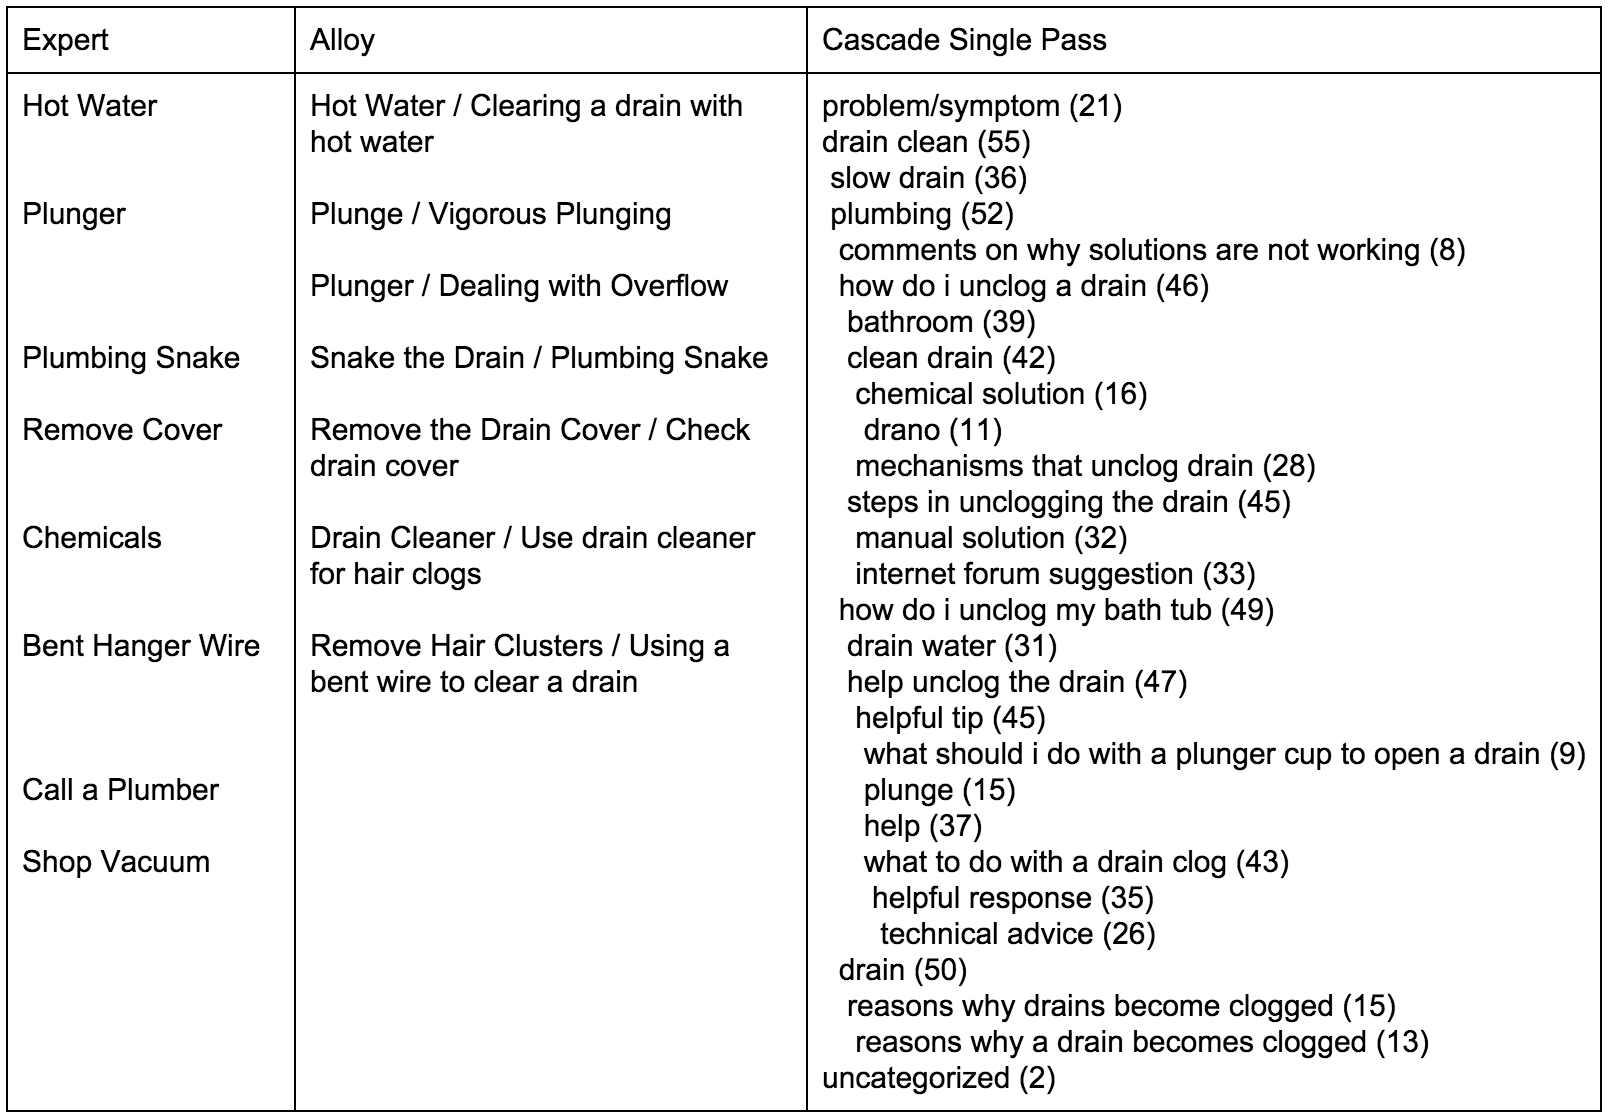
\includegraphics[width=0.9\columnwidth]{Chapters/Alloy/images/bathtub_cats.png}
	\caption{Categories comparison for Q1}
	\label{fig:bathtub_cats}
\end{figure}

%\begin{figure}
%	\centering
%	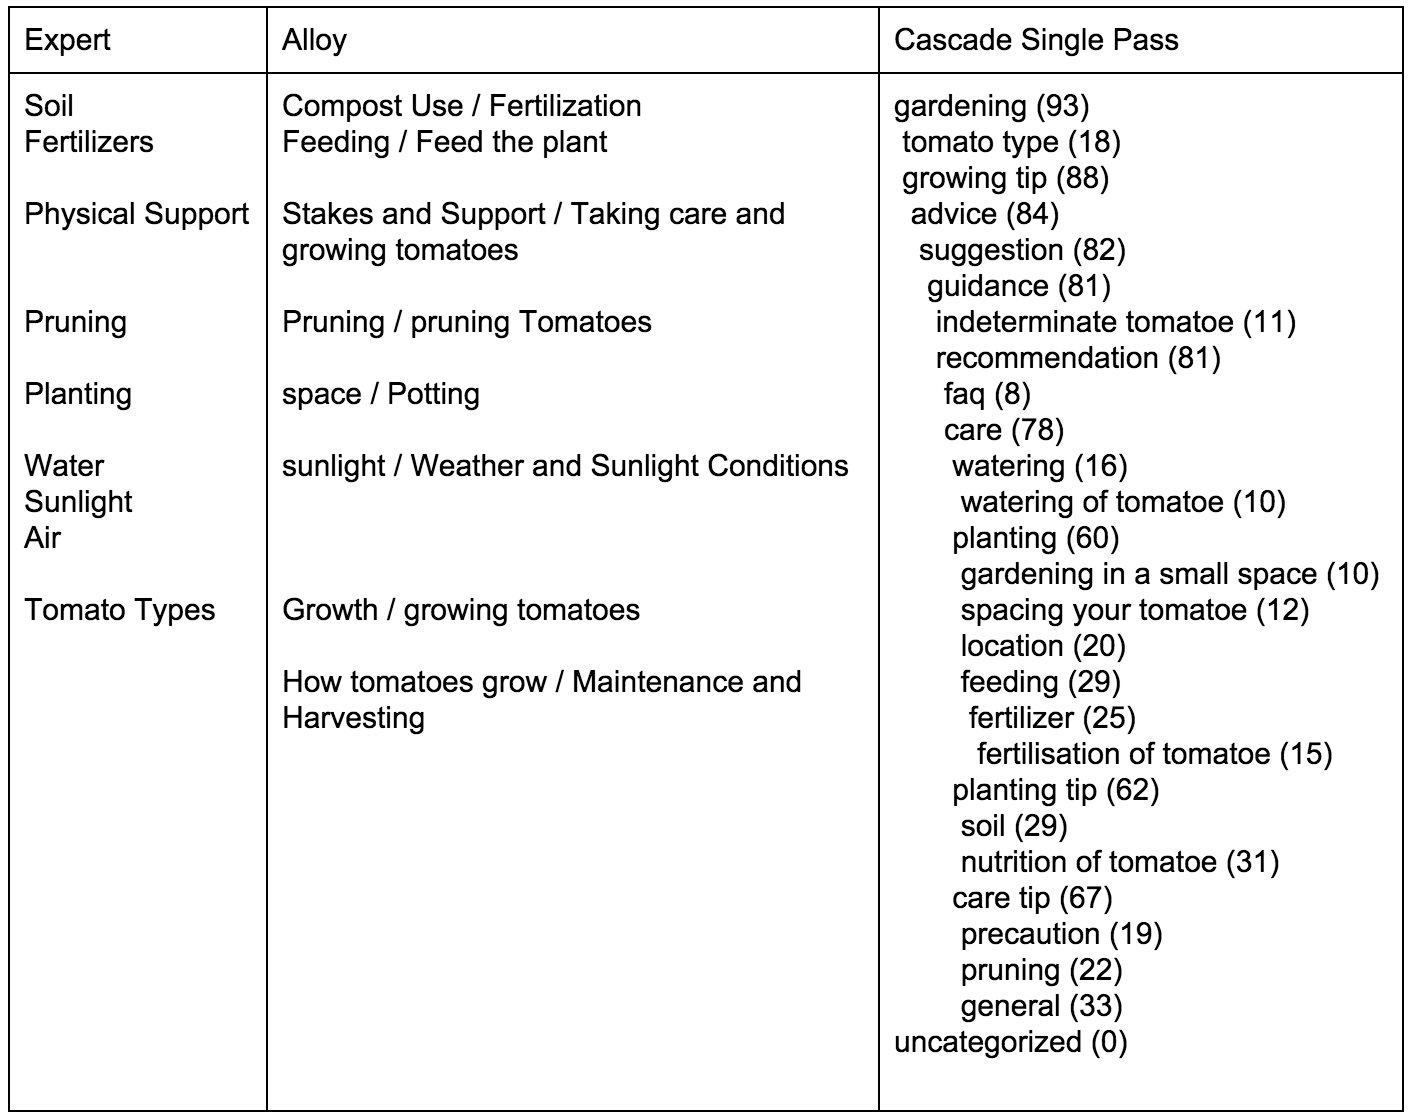
\includegraphics[width=0.9\columnwidth]{images/tomato_cats.png}
%	\caption{Categories comparison for Q2}
%	\label{fig:tomato_cats}
% \end{figure}

We compare Alloy with Cascade using datasets Q1-Q4, a popular crowd-based method for
discovering taxonomies in unstructured data based on overlapping crowd
clusters \cite{chilton2013cascade}.
We implemented a simplified version of Cascade using the parameters
described in the paper, but with only one recursion.  We acknowledge that fine
tuning and multiple recursion might improve Cascade's performance, but the
numbers from our evaluation are consistent with the results reported in the
Cascade paper based on the same metric and similar datasets.

On average, 84\% of categories generated with Alloy were shared with clusters
in the gold standard, versus 50\% for Cascade.  Cascade produced soft
clusters where child clusters did not necessarily have all the items included in
their parents, which breaks the assumptions of using NMI. To produce
a direct comparison, we use the gold standard to greedily extract best
matching, overlapping clusters that cover all items, and evaluated them using
the average F1. In essence, this simulates an omniscient ``oracle'' that gives
Cascade the best possible set of cluster matches, and so is perhaps overly
generous but we wanted to err on the conservative side. The average F1 scores
for each questions using Alloy are .72, .54, .48, .52, and using Cascade are
.50, .48, .42, .39, showing a consistent advantage across questions.
Furthermore, Alloy achieved this better performance at a
lower cost (average \$20 for Alloy vs \$71 for Cascade),
suggesting that machine learning can provide valuable scaling properties.
We show categories created by experts and elicited from the two systems
in Figure~\ref{fig:bathtub_cats} to give a better sense of the datasets and the output.
% and  Figure~\ref{fig:tomato_cats}. 

% \begin{table*}
%   \centering
% 
% \begin{tabular}{ |l|l|p{3in}| }
% \hline
% Expert & Alloy & Cascade Single \\
% \hline
% Hot Water & Hot Water / Clearing a drain with hot water & \\
% Plunger   & Plunge / Vigorous Plunging & \\
%           & Plunger / Dealing with Overflow & \\
% Plumbing Snake & Snake the Drain / Plumbing Snake & \\
% Remove Cover   & Remove the Drain Cover / Check drain cover & \\
% hemicals       & Drain Cleaner / Use drain cleaner for hair clogs & \\
% Bent Hanger Wire & Remove Hair Clusters / Using a bent wire to clear a drain & \\
% Call a Plumber & & \\
% Shop Vacuum & & 
% \multirow{-9}*{
% \begin{minipage}{3in}
% problem/symptom (21)\newline
% drain clean (55)\newline
% \hspace{1mm} slow drain (36)\newline
% \hspace{1mm} plumbing (52)\newline
% \hspace{1mm} \hspace{1mm}  comments on why solutions are not working (8)\newline
%   how do i unclog a drain (46)\newline
%    bathroom (39)\newline
%    clean drain (42)\newline
%     chemical solution (16)\newline
%      drano (11)\newline
%     mechanisms that unclog drain (28)\newline
%    steps in unclogging the drain (45)\newline
%     manual solution (32)\newline
%     internet forum suggestion (33)\newline
%   how do i unclog my bath tub (49)\newline
%    drain water (31)\newline
%    help unclog the drain (47)\newline
%     helpful tip (45)\newline
%      what should i do with a plunger cup to open a drain (9)\newline
%      plunge (15)\newline
%      help (37)\newline
%      what to do with a drain clog (43)\newline
%       helpful response (35)\newline
%        technical advice (26)\newline
%   drain (50)\newline
%    reasons why drains become clogged (15)\newline
%     reasons why a drain becomes clogged (13)\newline
% uncategorized (2)\newline
% \end{minipage}
% } \\[3.1in]
% \hline
% 
% \end{tabular}
%   \caption{Bathtub Categories}
%   \label{tab:bathtub_cats}
% \end{table*}




% \subsection{Crowdworkers}

% The crowdworkers employed to test the proposed method are recruited from Amazon
% Mechanical Turk. With a total of 65 unique workers participated in the
% experiments, 56 of them have IP addresses origin in the United States, 6 of
% them from India, and 3 from other regions. From self-reporting, 40 workers are
% males and 25 workers are females, 8 workers are between the age of 18 to 24, 40
% workers are between the age of 25 to 34, 15 workers are between the age of 35
% to 44, and the rest in other ranges or chose not to report. Each worker is paid
% 1.00 USD for completing one of the two HITs. Therefore, the costs for both
% Workflow2 and Workflow1 is 20.00 USD.

% \begin{table*}
%   \centering
% % question, number of sources, number of clips, number of turkers
%   \begin{tabular}{ c l l l l l }
%     \hline
% 	\tabhead{} &
% 	\tabhead{Phase A Mean} &
% 	\tabhead{Phase A Std. Dev} &
% 	\tabhead{Phase B Mean} &
% 	\tabhead{Phase B Std. Dev} &
% 	\tabhead{ANOVA P-Value} \\
%     \hline

% 	Interface & 4.2270 & 0.6477 & 3.710 & 0.783 & $\sim$ 0.000 \\ 
% 	Instructions & 4.0286 & 0.9592 & 3.786 & 1.001 & $\sim$ 0.156 \\
% 	Difficulty & 3.5099 & 1.0255 & 3.119 & 1.109 & $\sim$ 0.033 \\

%     \hline

%   \end{tabular}
%   \caption{Survey feedback from the crowdworkers.}
%   \label{tab:feedback}
% \end{table*}


% \subsection{Survey feedback from Crowdworkers}
% Upon completion of each HIT, we asked each unique worker to rate the task
% description, interface design, and overall difficulty of the HITs by filling
% out a survey form. We used a 5-point Likert scale, ranging from ``Strongly
% Agree'' (5) to ``Strongly Disagree'' (1) in order to gauge their opinions
% regarding the different features of the HIT. As shown in Table \ref{tab:feedback}, workers
% thought that the interface from Phase A was easier to utilize than interface
% for Phase B (p-value $\sim$ 0.000), with their average response being that they
% agreed that Phase A's interface was easy to use, while Phase B's interface
% was acceptable. There was not a significant difference between their responses
% regarding the instructions, agreeing that for both phases the instructions were
% easy to understand and follow. Finally, workers thought that Phase A was easier
% than Phase B (p-value $\sim$ 0.033), with neither task being considered to be
% particularly easy to complete. 

% We also allowed the Crowdworkers to comment on the HITs, and many of them find
% the clustering process interesting and enjoyable, leaving comments such as
% ``This was an interesting hit. I enjoyed it.'', ``very interesting to name each
% clusters'', and ``This was an interesting study and I actually learned a new
% tip to try and clear a clogged drain.'' 


%\begin{table*}
%  \centering
%% question, number of sources, number of clips, number of turkers
%  \begin{tabular}{ l r r r r r }
%    \hline
%	\tabhead{Questions} &
%	\tabhead{strongly agree} &
%	\tabhead{agree} &
%	\tabhead{neither...} &
%	\tabhead{disagree} &
%	\tabhead{strongly disagree} \\
%    \hline
%    \multicolumn{6}{c}{\tabhead{Phase A}} \\
%    \hline
%	% 54
%	\emph{I find this task easy to complete} & 11\% & 46\% & 31\% & 11\% & 0\% \\
%  
%	% 53
%	\emph{The instructions clearly explain the task} & 34\% & 55\% & 8\% & 4\% & 0\% \\
% 
%	% 54
%	\emph{The user interface is easy to learn and use} & 40\% & 56\% & 4\% & 0\% & 0\% \\
%    \hline
%    \multicolumn{6}{c}{\tabhead{Phase B}} \\
%    \hline
%	% 54
%	\emph{I find this task easy to complete} & 9\% & 45\% & 9\% & 36\% & 0\% \\
%
%	% 53
%	\emph{The instructions clearly explain the task} & 18\% & 55\% & 11\% & 11\% & 11\% \\
%
%	% 54
%	\emph{The user interface is easy to learn and use} & 27\% & 55\% & 11\% & 11\% & 0\% \\
%    \hline
%
%  \end{tabular}
%  \caption{Survey feedback from the crowdworkers.}
%  \label{tab:feedback}
%\end{table*}



\begin{figure*}
	\centering
	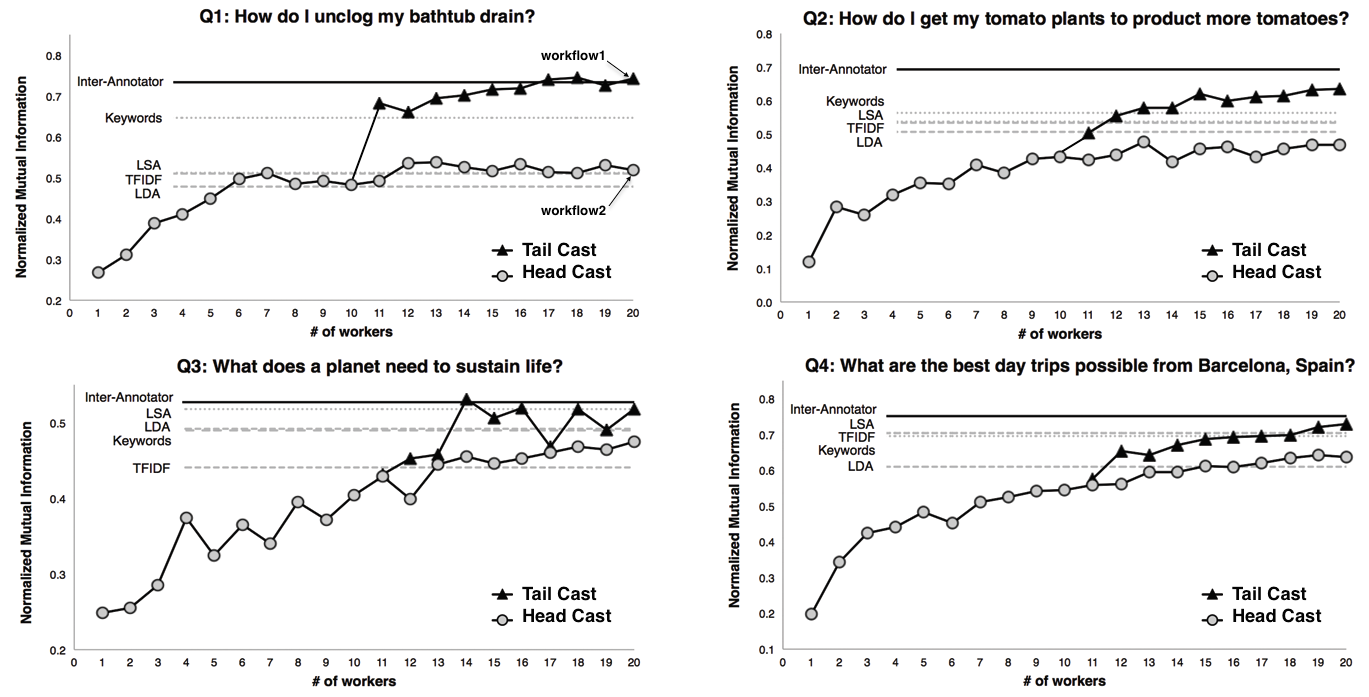
\includegraphics[width=1\columnwidth]{Chapters/Alloy/images/numberOfTurkers.png}
	\caption[Performance comparison of using different number of crowdworkers.]{Performance comparison of using different number of crowdworkers in the Head Cast and the Tail Cast.}
	\label{fig:numberOfTurkers}
\end{figure*}


\subsection{Experiment 2: Robustness}
%!TEX root = main.tex


\footnotetext[1]{We also evaluated Q1 and Q2 using the AMI metric that accounts
    for randomness.  The inter-annotator agreements are .674 and .643,
    respectively, and Alloy performed .674 and .609, respectively. See the
    Evaluation Metric Section for detail.}

% \textbf{Workflow2: $Head Cast$}
% \vspace{-2mm}

In this section, we examine the robustness of
Alloy by varying the number of crowdworkers employed in the Head and the Tail Cast on datasets Q1-Q4. We start
with having only 1 worker in the Head Cast, and evaluate performance as we hire more
workers until we have 20. To test the two phase assumption, in a second
condition, we switch to the Tail Cast after hiring 10 workers in the Head Cast,
and continue to hire 1 to 10 more workers.
This way, we can characterize the cost/benefit trade-offs in hiring different amount of human
judgments. Further, by omitting the Tail Cast completely 
in the first condition, we can verify
the two phase assumption by comparing the performance of a two-phase process
(Head Cast and Tail Cast) with a one-phase control (Head Cast only) while equaling
the number of workers:

\begin{itemize}
    \setlength\itemsep{0.0em}
	\item \emph{Workflow1}. The workflow with ten crowdworkers each for
		the Head Cast and the Tail Cast. Each HIT costs 1 USD.
	\item \emph{Workflow2}. The workflow with twenty crowdworkers and
		the Head Cast only. Each HIT costs 1 USD.
\end{itemize}

In addition, to test how robust Alloy is to the variance of crowdworkers on Amazon Mechanical Turk, 
we also hired eleven sets of ten different crowdworkers (a total of 440) for each 
Head and Tail Casts for Q1 and Q2. 

\subsubsection*{Results}


In Figure~\ref{fig:numberOfTurkers}, we show the performance of
employing different number of workers in the Head and the Tail Cast.  Initially,
increasing the number of workers in the Head Cast shows significant
performance improvements.  However, after gathering training data from around 10 
workers, the performance gain from hiring additional
crowdworkers decreases notably. Instead, performance improved significantly
even with only a few additional crowdworkers in the Tail Cast to refine
the clusters. Overall, 
having
10 crowdworkers in each of the Head and Tail Cast consistently outperformed having all
20 crowdworkers in the Head Cast across all four questions (Table~\ref{tab:results}),
suggesting there is significant value in the Tail Cast.

For Q1 and Q2, we also ran Alloy eleven times using different
crowdworkers, and compared the results against the gold-standard labels and also with
each other. Comparing to the gold-standards, which have inter-annotator
agreements of $.734$ and
$.693$ for Q1 and Q2 respectively, Alloy produced an average NMI of .759 (SD=.016) and .687 (SD=.016), respectively.
Further, the average pair-wise NMI score of the 11 runs are .819 (SD=.040), and .783 (SD=.056), respectively, suggesting Alloy
produces similar results using different crowdworkers on the same datasets.

%Further, the average pair-wise NMI score of the four conditions (Head Cast Q1, Q2, and Tail
%Cast Q1, Q2) are .740 (SD=.106),
%.758 (SD=.088), .819 (SD=.040), and .783 (SD=.056). This suggests Alloy
%produces similar results using different crowdworkers on the same dataset. 



\subsection{Experiment 3: Other Datasets}
%!TEX root = main.tex

% \textbf{Workflow1:} $HeadCast \rightarrow MergeCast \rightarrow TailCast$
% \vspace{-2mm}

%Alloy was initially designed to organize corpora of ideas that answer a specific questions described using short text clips.
In this experiment, we use the same distributed workflow to test Alloy 
using the Wiki and CSCW datasets as described in the Dataset Section, in order
to test how Alloy generalizes to other types of data. These datasets contain long
academic documents or editorial discourses that are infeasible to present multiple items to the crowdworker in one HIT.
Instead, we show a small portion of each item in the datasets to the crowdworkers.
For each item
in the Wiki dataset, we display the thread-starter post and the first two replies. For the CSCW dataset,
we present the abstract
section of each paper, and compare results with the official conference sessions. Machine baselines were however given
access to all of the text of the paper and the full discussion threads in order to provide a strong test of Alloy's approach.

%\niki{move this to discussion if you want}
%We acknowledge that organizing long documents is a limitation of Alloy.
%However, this limitation also presents in most previous crowd-based approaches.

\subsubsection*{Results}

% \subsubsection{CSCW Conference Papers}

For the CSCW dataset, Alloy outperformed all machine baseline
systems with \emph{.748} NMI score using conference sessions as the gold standard Table~\ref{tab:results}.
The Keyword baseline outperformed the TF-IDF baseline (\emph{.652} vs \emph{.584}), showing
that the crowdworkers are extracting valuable keywords in the Head Cast, despite that
research papers may be difficult or impossible for crowdworkers to understand. On the other hand,
Alloy produced 24 categories out of 135 abstracts, more than all other datasets. One possible
assumption is that it may be more difficult for novice workers to induce abstract categories
when organizing expert dataset, leading to higher number of more lower level categories in
the outcome.

% Note that even though only the abstract sections were available to the crowdworkers,
% we used the full articles as the input to the baseline systems to improve their performance,
% and explored multiple parameter settings report their best results.

% \subsubsection{Wikipedia Editor Discussion Threads}

For the Wiki dataset, the NMI score between annotators was \emph{.604}, which is comparable
to the two other large datasets Q5 and Q6. Comparing to the two sets of expert
labels independently, Alloy's output measured \emph{.528} and \emph{.507}.
Compared to all previous results, Alloy seemed to perform less favorably on this
dataset. As mentioned in the Dataset Section, the raters found the this dataset the most
difficult to organize, as there are many different valid structures that the two
annotators were unable to reach an agreement 
also hints that the space of valid solutions may be larger on this dataset. 
In addition, we only showed the first three comments of
each discussion to the crowdworkers, whereas the annotators and the machine baselines
have access to the full discussion. 
We acknowledge length of items is a limitation, and will discuss in detail in
the Discussion Section.

%This is potentially a substantial disadvantage to
%Alloy, as the full discussions can contain up to more than a hundred comments.
%Unlike the abstracts of research papers, the first three comments might not be
%representative enough of the discussions.




\section{Application: \textbf{Knowledge Accelerator}}
\label{chap:ka}

{\rmfamily
This work was previously published in ACM SIGCHI 2016 \cite{ka} and has been adapted for this document.
}

\begin{figure}
    \centering
    \frame{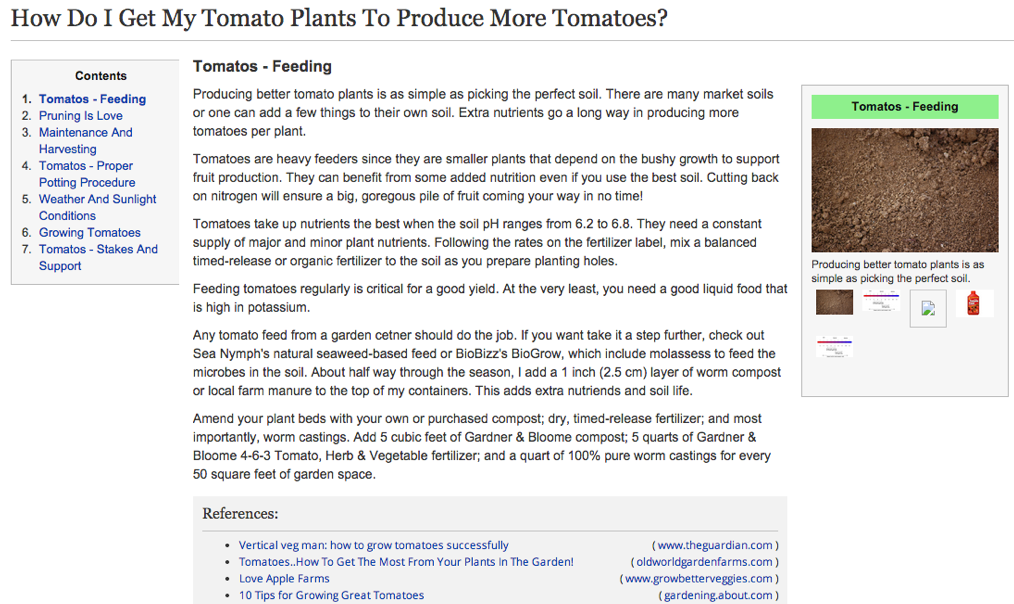
\includegraphics[width=1\columnwidth]{Chapters/KA/final_answer}}
    \caption[Alloy clusters synthesized into a report articles using the Knowledge Accelerator.]{Example report synthesized by the Knowledge Accelerator system. The table of content on the left listed cluster names generated from Alloy, each corresponded to a different section in the report.}
    \label{fig:final_answer}
\end{figure}

\begin{figure}
    \centering
    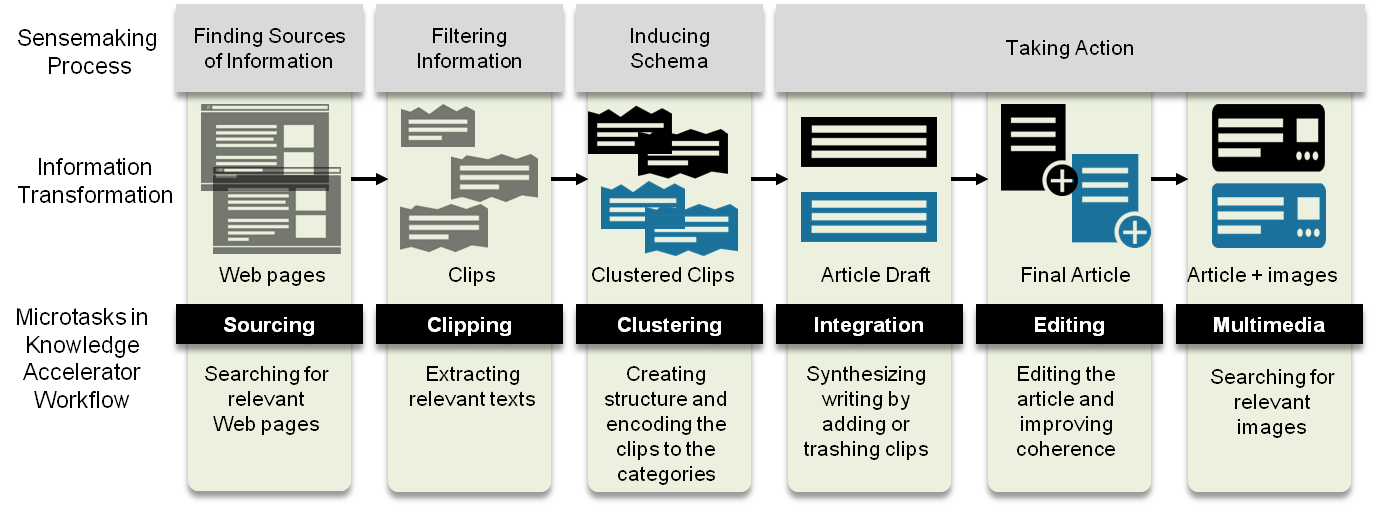
\includegraphics[width=1\columnwidth]{Chapters/KA/overview}
    \caption[The Knowledge Accelerator (KA) with Alloy as the Clustering Stage.]{The process of the Knowledge Accelerator (KA). Alloy is used for the Clustering Stage of the pipeline.}
    \label{fig:process}
\end{figure}


To evaluate the usefulness of structures generated by Alloy in a more realistic scenarios, we first used Alloy to clusters a larger set of information seeking datasets (Table~\ref{tab:evaluation}) collected using the same procedure as described in \cref{chap:info_seek_datasets}. We then developed a prototype system called the ``Knowledge Accelerator'' (KA) to synthesize the output of Alloy into articles. Each of the cluster produced by Alloy corresponds to a different section in an article. An example of the output of the system for the target question ``How do I get my tomato plants to produce more tomatoes?'' can be found in Figure~\ref{fig:final_answer}.

In addition, the KA system probes how to accomplish a complex information synthesis task entirely through relatively small contributions. We limited our maximum task payment to \$1 US, aimed at incentivizing a Target task time of approximately 5-10 minutes. Critically, the KA system accomplishes this process without a core overseer or moderator. Figure \ref{fig:process} shows the overview of the KA System with Alloy being the Clustering Stage. For more details on the KA system refer to \cite{ka}.

We evaluated the usefulness and coherence of the articles by comparing them against webpages an individual might use if they were to complete the same tasks without KA and Alloy --- Top Google search results that consists of expert-written articles published by trusted sources such as CDC.gov or the New York Times, as well as popular online forums such as TripAdvisor and Yahoo Answers.

\subsection{Experimental Settings}

Eleven topics were selected for evaluation by browsing question and answer forums, Reddit.com, and referencing online browsing habits \cite{pewReport}. For questions Q3 and Q8 we added additional constraints (i.e., having kids and age) to test the performance of the system for more personalized questions.
To compare the two conditions, participants were recruited through the Amazon Mechanical Turk US-only pool and paid \$1.50 for rating two webpages. Each participant was randomly assigned an output article from KA and a top search result webpage for the same topic (Figure~\ref{fig:aggregated}), and rate both webpages based on six criteria using 7-point Likert scale questions and provided free-form explanations: \emph{comprehensiveness}, \emph{confidence}, \emph{helpfulness}, \emph{trustworthiness}, \emph{understandability}, and \emph{writing}. We averaged ratings on these dimensions into a single score representing the overall perceived quality of the page.


\begin{table}
  \centering
  \footnotesize
% question, number of sources, number of clips, number of turkers
  \begin{tabular}{l r l}

	Question &
	\multicolumn{1}{c}{N} &
    \multicolumn{1}{c}{Score} \\
    \hline
	% 102
	\multicolumn{1}{p{0.75\columnwidth}}{\textbf{Q1}: \textit{How do I unclog my bathtub drain?}}
	& 116 & ~0.292 * \\

	% 115	
	\multicolumn{1}{p{0.75\columnwidth}}{\textbf{Q2}: \textit{How do I get my tomato plants to produce more tomatoes?}}
	& 177 & ~0.420 * \\

	% 153
	\multicolumn{1}{p{0.75\columnwidth}}{\textbf{Q3}: \textit{What are the best attractions in LA if I have two little kids?}}
	& 158 & -0.044 \\

	% 116
	\multicolumn{1}{p{0.75\columnwidth}}{\textbf{Q4}: \textit{What are the best day trips possible from Barcelona, Spain?}}
	& 98 & -0.109 \\

	% 177
	\multicolumn{1}{p{0.75\columnwidth}}{\textbf{Q5}: \textit{My Worcester CDi Boiler pressure is low. How can I fix it?}}
	& 139 & ~0.878 * \\

	% 168
	\multicolumn{1}{p{0.75\columnwidth}}{\textbf{Q6}: \textit{2003 Dodge Durango has an OBD-II error code of P440. How do I fix it?}}
	& 138 & ~0.662 * \\

	% 175
	\multicolumn{1}{p{0.75\columnwidth}}{\textbf{Q7}: \textit{2005 Chevy Silverado has an OBD-II error code of C0327. How do I fix it?}}
	& 135 & ~0.412 * \\

    % 160
	\multicolumn{1}{p{0.75\columnwidth}}{\textbf{Q8}: \textit{How do I deal with the arthritis in my knee as a 28 year old?}}
	& 139 & ~0.391 * \\

    % 161
	\multicolumn{1}{p{0.75\columnwidth}}{\textbf{Q9}: \textit{My Playstation 3 has a solid yellow light, how do I fix it?}}
	& 119 & ~0.380 * \\

    % 162
	\multicolumn{1}{p{0.75\columnwidth}}{\textbf{Q10}: \textit{What are the key arguments for and against Global Warming?}}
	& 138 & ~0.386 * \\

    % 163
	\multicolumn{1}{p{0.75\columnwidth}}{\textbf{Q11}: \textit{How do I use the VIM text editor?}}
	& 138 & ~0.180 \\
    \hline
    \multicolumn{3}{l}{\textbf{*} = significant at $p < 0.01$ after Bonferroni correction}\\

  \end{tabular}
  \caption[Comparing KA output with top websites for the eleven questions.]{Average difference between the KA output and top websites for the eleven questions (positive indicates higher ratings for KA, negative indicates higher ratings for the competing website). Each rating was an aggregate of 6 questions on a 7-point Likert scale.}
  \label{tab:evaluation}
\end{table}

\begin{figure}
    \centering
    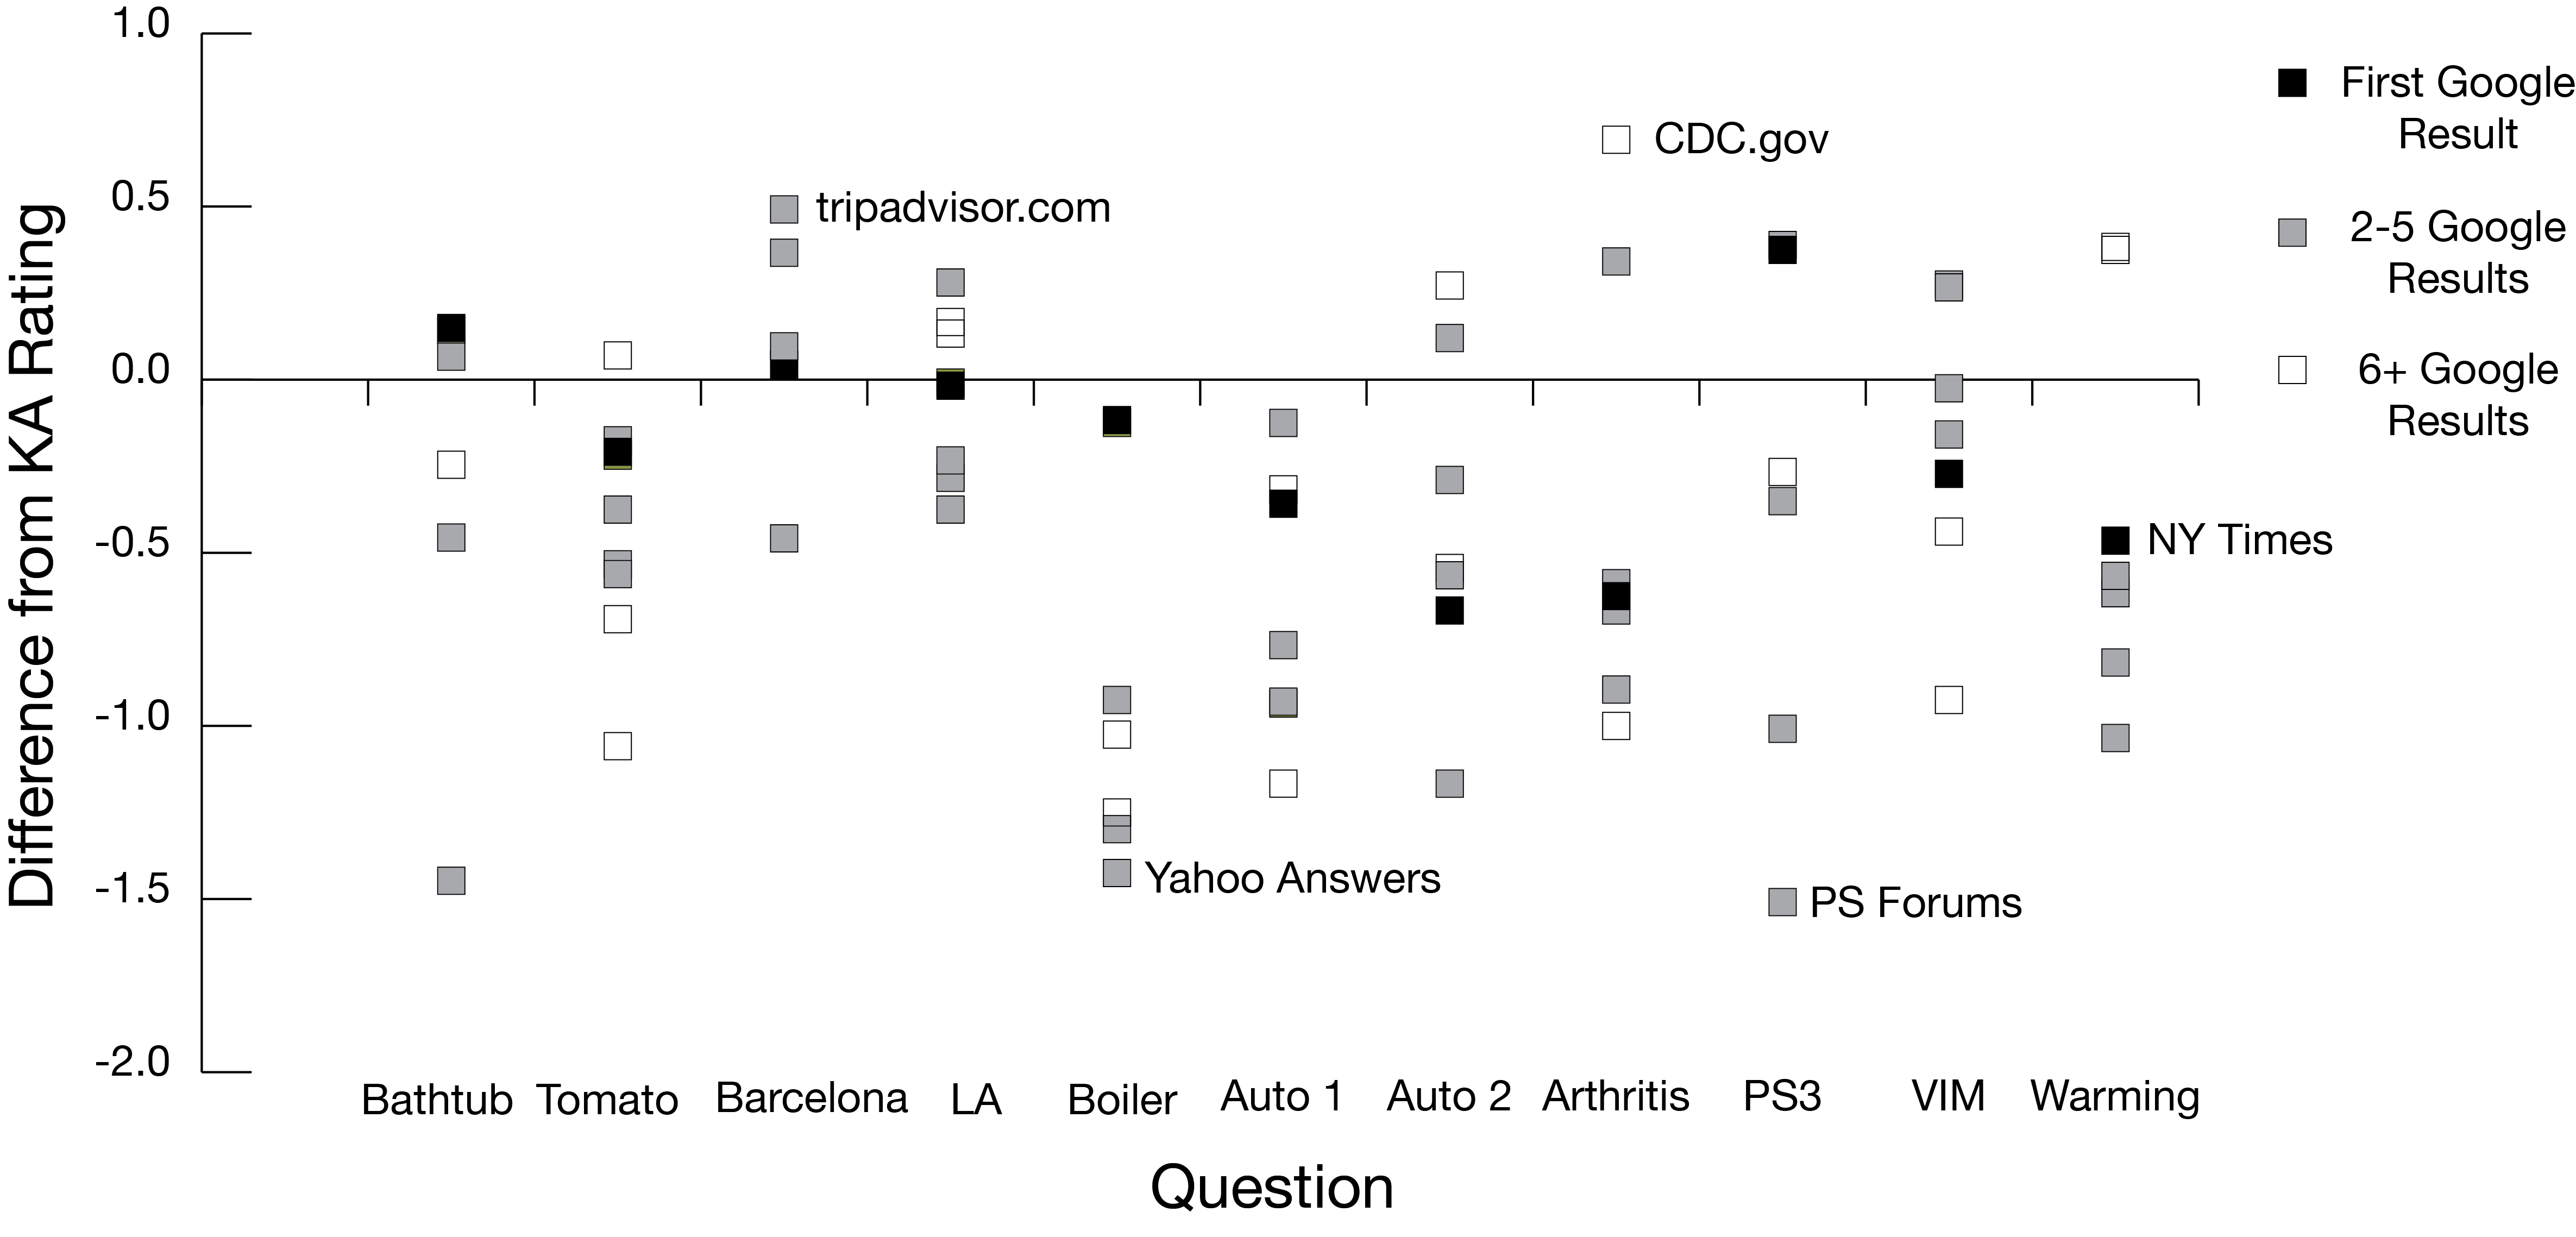
\includegraphics[width=1\columnwidth]{Chapters/KA/source_eval_graph}
    \caption[Results across questions and websites.]{Results across questions and websites. Points represent the average aggregate score difference between the KA answer and an existing site}
    \label{fig:aggregated}
\end{figure}

\subsection{Results}

\begin{table}
  \centering
  \small
% question, number of sources, number of clips, number of turkers
  \begin{tabular}{lrrr}
    \hline
    \textbf{Phase} & \textbf{Task Pay} & \textbf{Avg. \# of Tasks} & \textbf{Avg. Cost} \\
    \hline
	Sourcing & \$0.25 & 15 & \$3.75 \\

    Clipping & \$0.50 & 21.6 & \$10.80 \\

    Alloy Head Cast & \$1.00 & 10 & \$10.00 \\

    Alloy Merge + Tail Cast & \$1.00 & 10 & \$10.00 \\

    Integrate & \$0.50 & 37.2 & \$18.60 \\

    Edit 1 & \$0.75 & 28.8 & \$21.60 \\

    Edit 2 & \$1.00 & 28.8 & \$28.80 \\

    Images & \$0.50 & 9 & \$4.50 \\
    \hline    
    \textbf{Total} & & 160.4 & \$108.05 \\
    \hline
  \end{tabular}
  \caption[Average number of worker tasks and cost of running KA.]{Average number of worker tasks and average cost per phase, and overall, to run a question.}
  \label{tab:cost}
\end{table}

The costs of running a question through the KA system is shown in Table~\ref{tab:cost}. Across the 11 topics we tested, a full run with around 100 short text clips costed an average of \$108.50, of which around \$15 is spent on searching and extracting the text clips from webpages, \$20.00 is spent by the Alloy system, and the rest on synthesizing each of the Alloy clusters into a section in the final article and making sure the different sections are coherent.

Aggregating across all questions, KA output was rated significantly higher than the top 5 Google results (KA: $\bar{x} = 2.904$ vs Alt. Sites: $\bar{x} = 2.545$, $t(1493) = 13.062$, $p < 0.001$). An analysis of individual questions corrected for multiple comparisons is shown in Table~\ref{tab:evaluation}. 

The strongly positive results found were surprising because some of the websites in the comparison set were written by experts and had well-established reputations. Only on the two travel questions, Barcelona ($\bar{x} = -0.109$) and LA ($\bar{x} = -0.044$), and the VIM question ($\bar{x} = 0.180$) did the KA output not significantly outperform the comparison pages. A closer examination of these pages suggests that for the two travel questions, because of the strong internet commodity market surrounding travel, a considerable amount of effort has been spent on curating good travel resources. Even with the slightly more specific LA query, there were still two specialized sites dedicated to attraction for kids in LA (Mommypoppins.com and ScaryMommy.com). The VIM question represented a mismatch between our output and the question style. A number of the sources for the question were tutorials, however in the clipping phase, these ordered tutorials were broken up into unordered clips, creating an information model breakdown. This points out an interesting limitation in the KA approach, and suggests that adding support for more structured answers (e.g., including sequential steps) could be valuable future work. 


%As an additional external evaluation, for the two questions (Q6 and Q7) related to automotive systems we compared the discovered categories from the KA system with two commercial knowledge service products generated by expert technicians. We compared the KA response's accuracy and comprehensiveness, and found that it discovered all the categories referred to in these two commercial products for each question. Furthermore, the categories from the KA output provided more categories not mentioned in the commercial product (average 2.5 categories from two commercial products, while average 9.5 categories from KA). We validated these additional categories with expert automotive professionals who evaluated them as also being plausible and reasonable for the given questions. There was one instance in which two distinct categories (Encoder Motor and Encoder Motor Sensor) from the commercial products were clustered into the single category named Encoder Motor Assembly in the KA output. However, the full text answer from the KA system for Encoder Motor Assembly did still contain these two sub-components with different repair procedures. 

%It may seem surprising that KA would work well for questions such as automotive error codes, where the response relies heavily on technical knowledge and jargon. On further inspection we believe this is because there are many online resources that have valuable information pertaining to these questions but are in unstructured and dialog oriented forms. Workers in the sourcing phase found rich sources of online information from many car enthusiast discussion forums, in which members tried to diagnose and help each other solve their automative problems. Although crowd workers may not understand the esoteric jargon of the automative domain, their understanding of grammar, semantics, and argument structure was sufficient to let them find, filter, cluster, integrate, and edit this domain-specific information. These results suggest a interesting avenue for future research leveraging human understanding of semantics and argument structure to extend crowdsourcing to process expert domain knowledge and to understand the limits of where such an approach breaks down.

%(see Figure~\ref{fig:feedback})



%\subsection{Discussion}

 \begin{figure}
 	\fbox{ \vbox{
 		\ttfamily
 		\footnotesize
 		
		\textbf{categories induced during clipping (without Alloy):}\\
 		Boil Water, use hot water, Plunger, try a snake, How to Remove drain stopper, bleach, Use Drano Max Gel, baking soda, drain, tips to unclog, problem, tools, research, internet research, ..., etc.
 		
 		\rule{\columnwidth}{0.1pt}
 		
 		\textbf{categories induced by Alloy:}\\
 		Hot Water, Plunge, Plunger, Snake the Drain, Remove the Drain Cover, Drain Cleaner, Remove Hair Clusters.
 		
 		\rule{\columnwidth}{0.1pt}
 		
 		\textbf{gold-standard categories:}\\
 		Hot Water, Plunger, Plumbing Snake, Remove Cover, Chemicals, Bent Wire Hanger, Call a Plumber, Shop Vacuum.
 	}}
 	\caption[Categories induced from different stages of KA.]{Categories induced from different stages for Q1: \textit{How do I unclog my bathtub drain?}}
 	\label{fig:delayed-structuring}
 \end{figure}

The strong performance of the system is perhaps surprising given that its output was generated by many non-expert crowd workers, none of whom saw the big picture of the whole, and Alloy is a core component that provided useful and coherent structures for producing the final report. Initially we had workers provide labels to categorize each clip, which we planned to use to develop a structure for the article. However, the lack of context of the bigger picture made these labels poorly suited for inducing a good structure. For example, in Figure~\ref{fig:delayed-structuring} the top box shows the category structure induced by crowdworkers during clipping and without using Alloy during clipping, categories induced using Alloy, and gold standard categories developed by two independent annotators with access to all clips and sources, respectively. Categories induced without using Alloy matched poorly with the gold standard categories, and include categories with very different abstraction levels (e.g., \textit{Use Drano Max Gel} vs \textit{tips}). On the other hand, Alloy produced categories that were more coherent and matched more with gold-standard categories.

While we do not believe that this should be interpreted as a replacement for expert creation and curation of content, instead, the power of the system may actually be attributable to the value created by those experts by generating content which the crowd workers could synthesize and structure into a coherent digest. This explanation suggests that the approach would be most valuable where experts generate a lot of valuable information that is unstructured and redundant, such as the automative questions in which advice from car enthusiasts was spread across many unstructured discussion forums. In contrast, KA's output did not outperform top web sources for topics such as travel, where there are heavy incentives for experts to generate well structured content.  We believe its performance is likely due to its aggregation of multiple expert viewpoints rather than particularly excellent writing or structure per se, never the less, the KA system showcased that the structures produced by Alloy can be synthesized into coherent articles that were useful for exploratory searchers.



\section{Discussion}
%!TEX root = main.tex


In this chapter, we took a step towards tackling
the problem of clustering high-dimensional, 
short text collections by combining techniques from natural language processing and
crowdsourcing.  By using a two-phase process connected by a machine learning backbone,
our proposed method compensates
for the shortcomings of crowdsourcing (e.g., lack of context, noise) and
machine learning (e.g., sparse data, lack of semantic understanding). As part of the system we introduced an approach aimed at providing greater context to workers by transforming their task from clustering fixed subsets of data to actively sampling and querying the entire dataset. 

We presented three evaluations that suggest Alloy performed better 
and more consistently than automatic
algorithms and a previous crowd method in accuracy with 28\% of the cost
(Exp.1), is robust to poor work with only 20 workers (Exp.2),
and is general enough to support different types of input (Exp.3).
Qualitatively, we noticed Alloy often produced better names for categories than
machine algorithms would be capable of, including names not in the text (e.g., a cluster 
including items about \emph{smart thermostats} and \emph{solar panels} was
named ``\emph{Home Improvements}'' which was not in the actual text).

% On average, Alloy produced results
% with .623 against the gold-standards, .023 lower than the inter-annotator
% agreement,
%which is higher than all four baseline systems that ranged from
% .503 to .554 (Table~\ref{tab:results}).

%The first experiment shows that based on
%manually created gold-standard data outperformed four automatic /
%semi-automatic baseline systems, and produced clusters with normalized mutual
%information scores comparable to human inter-annotator agreement.  
%Alloy also performed better comparing to state-of-the-art crowd-based method 
%on accuracy using 28\% of the cost.
%Compared to some previous crowd-based methods, which rely on earlier
%crowdworkers to conceptualize or generate categories for each items based on
%limited context, our method based on crowdworkers ``voting'' on whether each
%item pair should be in the same cluster is less prone to a few workers making
%bad judgements or creating general but not informative clusters (e.g.,
%\emph{answers} or \emph{tips}). Previous methods also suffer from scaling
%problems as they require each item to be labeled by at least one crowdworker.
%In Phase A of the proposed method, we employ crowdworkers to select salient
%keywords from a small set of clips as general features that can be
%used to cluster clips that are not seen by any crowd worker.
%
%In the second experiment, we test the robustness and the strength of the
%two-phase approach of the proposed method by using different number of
%crowdworkers at different phases. Results show even with only a few workers in
%the second phase can significantly improve the performance. In the third
%experiment, we showed that the distributed version of Alloy can produce
%similar performance on significantly larger datasets.  
%
%In the final experiment, we showed that Alloy can support datasets beyound
%information seeking, by evaluating against datasets extracted from Wikipedia
%and a research conference. Results show that the proposed method is able to
%organize expert documents evaluated based on conference sessions, but not as
%good on Wikipedia editor discussions.


% (limitations)
% we may want to discuss limitations such as how would we scale to very large
% bodies of text or larger documents than snippets, also supporting multiple
% classification and hierarchy.

%\subsection{Limitations and Future Work}

One potential concern might be whether Alloy's tasks take too long to be considered microtasks. 
While Alloy deploys HITs that take more than a few
seconds to finish, we think they are still comparable to other complex microtask systems
such as Soylent \cite{bernstein2010soylent} and CrowdForge \cite{kittur2011crowdforge}.
Specifically, based on a total of 281 HITs, the median run-time
for the Head Cast HITs is 7.5 minutes (M=8,3, SD=4.1), for
Merge Cast 8.3 minutes (M=16.2, SD=15.6), and for Tail Cast
11.4 minutes (M=13.2, SD=6.1). 
Despite having less workers
doing longer tasks, Alloy performed consistently
across different sets of workers on the same datasets.


During development, some assumptions, both explicitly
and implicitly, were made about the input of the system:
1) there are more clips than categories.
2) the categories follow a long-tailed distribution.
3) clips belong to primarily one cluster.
4) there is a small set of gold-standard clusters.
5) workers can understand the content enough to cluster it.
Note that we do not assume the crowdworkers can understand the semantics of the
content, but just enough to identify ideas that are salient and common in the
dataset.
Thus they may be able to cluster complex topics such as machine learning without
understanding those topics if enough relational context is embedded in the clips.
For example, an abstract of a research paper may say ``this paper uses POMDP
machine learning
approaches to cluster text'', they might put it in a ``clustering''
cluster without
knowing what a POMDP is.

% \begin{enumerate}
%     \setlength\itemsep{0.1em}
% 
%     \item there are many more clips than categories.
%     \item the categories follow a long-tailed distribution.
%     \item clips belong to primarily one cluster.
%     \item there is a small set of gold-standard clusters.
%     \item workers can understand the content enough to cluster it.
% \end{enumerate}

One obvious limitation to our approach is clustering long documents.
This is a common limitation for crowd-based systems that rely
on workers reviewing multiple items for context
(either from random selection or active sampling). It becomes infeasible to fit multiple
items in a single HIT if the length of each item is long.
Another related limitation is organizing documents that describe multiple topics. 
Lab studies in a past work \cite{kittur2013costs}
showed that individuals are able to decompose long
documents into short clips of single topics during information seeking tasks. 
One way to expand the
proposed method to overcome the length limitation could be splitting documents into short
snippets, either with the crowds or machine algorithms,
and create topical clusters using Alloy.

% We can more formally characterize the scaling function on the number of categories shown in the Merge
% Cast as $T = log_c~N$, where $c$ represents the sparseness parameter of a dataset, $N$ the number of items 
% in the dataset, and $T$ the number of categories shown in the Merge Cast. The upper-bound limitation of 
% Alloy is then $T < L$, where $L$ is a limit on the complexity of a task given the characteristics of the 
% human computation platform utilized. Intuitively, this means that the Merge Cast will scale better 
% when the dataset involves fewer categories that explain more of the data, and when the human computation 
% platform supports more complex tasks.

% If we formulate the sparseness parameter $c$
% of a dataset base on the number of items $N$
% and the number of categories $T$ as $T = log_c ~ N$, the limitation of the distributed Merge Cast is 
% then $\ell \ge T$, where $\ell$ is the cognition limit of number
% of categories that can be presented in a single post to the given crowdsourcing marketplace.

Another limitation is organizing datasets that are inherently difficult to structure categorically. For example, 
concepts in Q3 (\emph{planetary habitability}) have causal relationships without
clear categorical boundaries (e.g., \emph{distance to sun}, \emph{temperature} and \emph{liquid water}).
As a result, all approaches had significant trouble,
including low agreement between human annotators. 
On the other hand, some dataset can be organized categorically in multiple ways.
In Q4 (\emph{Barcelona}) we found that some categories fit a \emph{place}
schema (e.g., \emph{Sitges}, \emph{Girona}) while other categories fit a \emph{type}
schema (e.g., \emph{museums}, \emph{beaches}).
One approach for addressing this could be trying to cluster workers to separate the different kinds of schemas; however, upon inspection we found that individual
workers often gave mixtures of schemas. This interesting finding prompts further research to investigate what cognitive and design features may be causing this, and how to learn multiple schemas. 
%One possible explanation is that a single schema often only covers part of the dataset,
%and we require the workers to organize all given items. For example, the $tool$ schema
%covers majority of the items in Q1 (bathtub drain), but does not cover items that
%explains how
%drains works, safety precautions, or steps to remove drain covers. 
%Another assumption is that information on the original sources are organize in different %ways, 
%and may influence the workers to use multiple schemes. 
%One possible improvement is to explicitly assign schemes to different workers, 
%and allow them to only cluster items that fits the given scheme. 
%A more interesting direction may be discovering a set of good schema using the crowd. 


% By examining the data, we found two reasons.  First,
% there is a lot of uncertainty in the topic, because not even the science
% community has a clear idea of the answer; for example, some clips even discussed whether
% the definition of life should be exclusively carbon based. Second, there are a
% lot of interconnected and correlated factors. For example, the \emph{distance
% 	to its star} determines whether a planet is in the \emph{habitable zone} of
% a solar system, which effects the \emph{temperature} of the planet and whether
% it potentially contains \emph{liquid water}. 


Looking forward, we identified a set of patterns that may be useful to system designers
aiming to merge human and machine computation to solve problems that involve rich
and complex sensemaking.
%  Our two-phase clustering approach breaks up human involvement
%  such that early workers can focus on building up context and finding common and
%  salient patterns in the data which are useful for training machine learning
%  classifiers, while later stage workers can leverage this previously
%  generated context (in the form of already created categories) to focus on the
%  edge cases and one-offs.
The hierarchical clustering backbone we use to integrate judgments from a
variety of crowdworker tasks allows us to \textit{cast} for different types of
crowd judgments and \textit{gather} them into a coherent structure that
iteratively gets better with more judgments.  We also introduce useful new
patterns for improving global context through self-selected \emph{sampling} and
keyword \emph{searching}.  One important consideration these patterns bring up
is that while previous ML-based approaches to crowd clustering have focused on
minimizing the number of judgments, we have found it is at least as important
to support the rich context necessary for doing the task well and setting up
conditions that are conducive for crowdworkers to induce meaningful structure
from the data.


We hope the patterns described in this chapter can help researchers
develop systems that make better use of human computation in different domains and for different purposes. For example,
the \emph{sample and search} pattern could potentially be adapted to support other tasks such as image
clustering, where crowdworkers could use the sampling mechanism to
get a sense of the variety of images in the dataset, highlight discriminative objects, and label images queried based on features extracted from the highlighted regions. Furthermore, the \emph{cast and gather} 
pattern may provide a useful framework for combining
crowds and computation that is both descriptive and generative. For example, Zensors \cite{laput2015zensors}, a crowd-based real-time video event detector, could be considered a form of the cast and gather pattern which uses a classification algorithm instead of a clustering algorithm as a backbone, and casts for human judgements whenever its accuracy falls below a threshold (e.g., if an environmental change lowers precision), with the classifier backbone retrained with the new human labels. While we used a clustering backbone in this work, 
future system designers might consider other machine learning backbones (e.g., classification or regression algorithms) for different tasks. Overall, we believe this approach takes a step towards solving complex cognitive tasks by enabling better global context for crowd workers and providing a flexible but structured framework for combining crowds and computation.


% Many other future research directions present themselves. For example, we can
% improve quality by using the crowd to fuse similar dimensions together by highlighting
% synonymous words to improve quality. On the other hand, we can push the boundary of crowd-clustering methods by testing Alloy on typical machine learning datasets that have significantly more items. 
% Other computational techniques could be used to optimize Alloy to require
% less human labor. For example, techniques in \cite{bragg2013crowdsourcing}
% can potentially be adapted to dynamically determine when to stop hiring more
% crowdworkers in each Cast. Alternatively, 
% the random sampling mechanism in the Head Cast could be replaced by
% active learning techniques; for example, presenting the most uncertain
% clips to crowdworkers for precision, or clips with fewer annotations or
% those that do not contain previously highlighted keywords for coverage. 

% Finally, we hope that Alloy can motivate new research that focuses on
% combining computation and crowdsourcing to tackle problems that are
% difficult for individual or machine algorithms,
% and the proposed design patterns can be helpful for
% other researcher when building future crowd-based information systems.


% On the other hand, scalling of number of snippets can be achieved through
% crowdworkers working on a smaller set of random clips, as shown in Phase B.
% There is no apparent way to scale the system to cover datasets that are both
% huge in number of clips and number of categories in Phase B. Since it could be
% difficult to cover all categories as each crowdworker can only process a small
% number of clips.

% \jeffrz{One final sentence here to end on a high note and get people excited again}



%\section{Acknowledgements}
%The authors would like to thank to Andrew Peters for the valuable discussions.
%This work was supported by NSF grants IIS-1149797, IIS-0968484, IIS-1111124, Bosch, and Google. 



\Chapter{Revolt}{Exploiting Disagreements For Concept Evolution in Crowd Labeling}
\label{chap:revolt}

{\rmfamily
This work was previously published in ACM SIGCHI 2017 \cite{Chang:2017:Revolt} and has been adapted for this document.
}

This chapter describe the second of the two crowd systems in this dissertation that explored ways to provide global context in sourced data exploration. Unlike Alloy that focused on providing global context to the crowdworkers who were constraint by their capacity to process large amounts of data in microtasks, this second system focused on providing global context to the requesters who typically turned to crowdsourcing for its ability to scale to large datasets that they themselves do not have the capacity to process fully.
Here I focused on another common approach of data analysis of labeling items in a dataset with predefined categories, a crucial process for generating labels for training machine learning models.
Crowdsourcing provides a scalable and efficient way to construct labeled datasets for training machine learning systems. However, creating comprehensive label guidelines for crowdworkers is often prohibitive even for seemingly simple concepts. Incomplete or ambiguous label guidelines can then result in differing interpretations of concepts and inconsistent labels. Existing approaches for improving label quality, such as worker screening or detection of poor work, are ineffective for this problem and can lead to rejection of honest work and a missed opportunity to capture rich interpretations about data. We introduce \emph{Revolt}, a collaborative approach that brings ideas from expert annotation workflows to crowd-based labeling. Revolt eliminates the burden of creating detailed label guidelines by harnessing crowd disagreements to identify ambiguous concepts and create rich structures (groups of semantically related items) for post-hoc label decisions. Experiments comparing Revolt to traditional crowdsourced labeling show that Revolt produces high quality labels without requiring label guidelines in turn for an increase in monetary cost. This up front cost, however, is mitigated by Revolt's ability to produce reusable structures that can accommodate a variety of label boundaries without requiring new data to be collected. Further comparisons of Revolt's collaborative and non-collaborative variants show that collaboration reaches higher label accuracy with lower monetary cost.\cite{Chang:2017:Revolt}

%\saleema{Is it true that there is an increase?} \joseph{there is an increase in worktime. i think its fair to admit this since there is extra work (explain, categorize) in our crowd workflow. i added 'monetary' here to make it more clear.} \saleema{I'll come back to this after I go through the results section. From what I remember, one of the asynchronous variants incurred a higher cost because we required people to explain all items, not just ambiguous ones...}
%We also compare Revolt to asynchronous variants of our approach showing the benefit of real-time collaboration for reducing cost and increasing label quality. \saleema{Rephrase given async issue}\ece{Maybe rephrase the last sentence like this: Comparisons of real-time and asynchronous versions of Revolt highlight trade-offs between accuracy and cost; real-time collaboration reaching higher label accuracy in term for increased costs.}



\begin{figure}[ht]
	\centering
	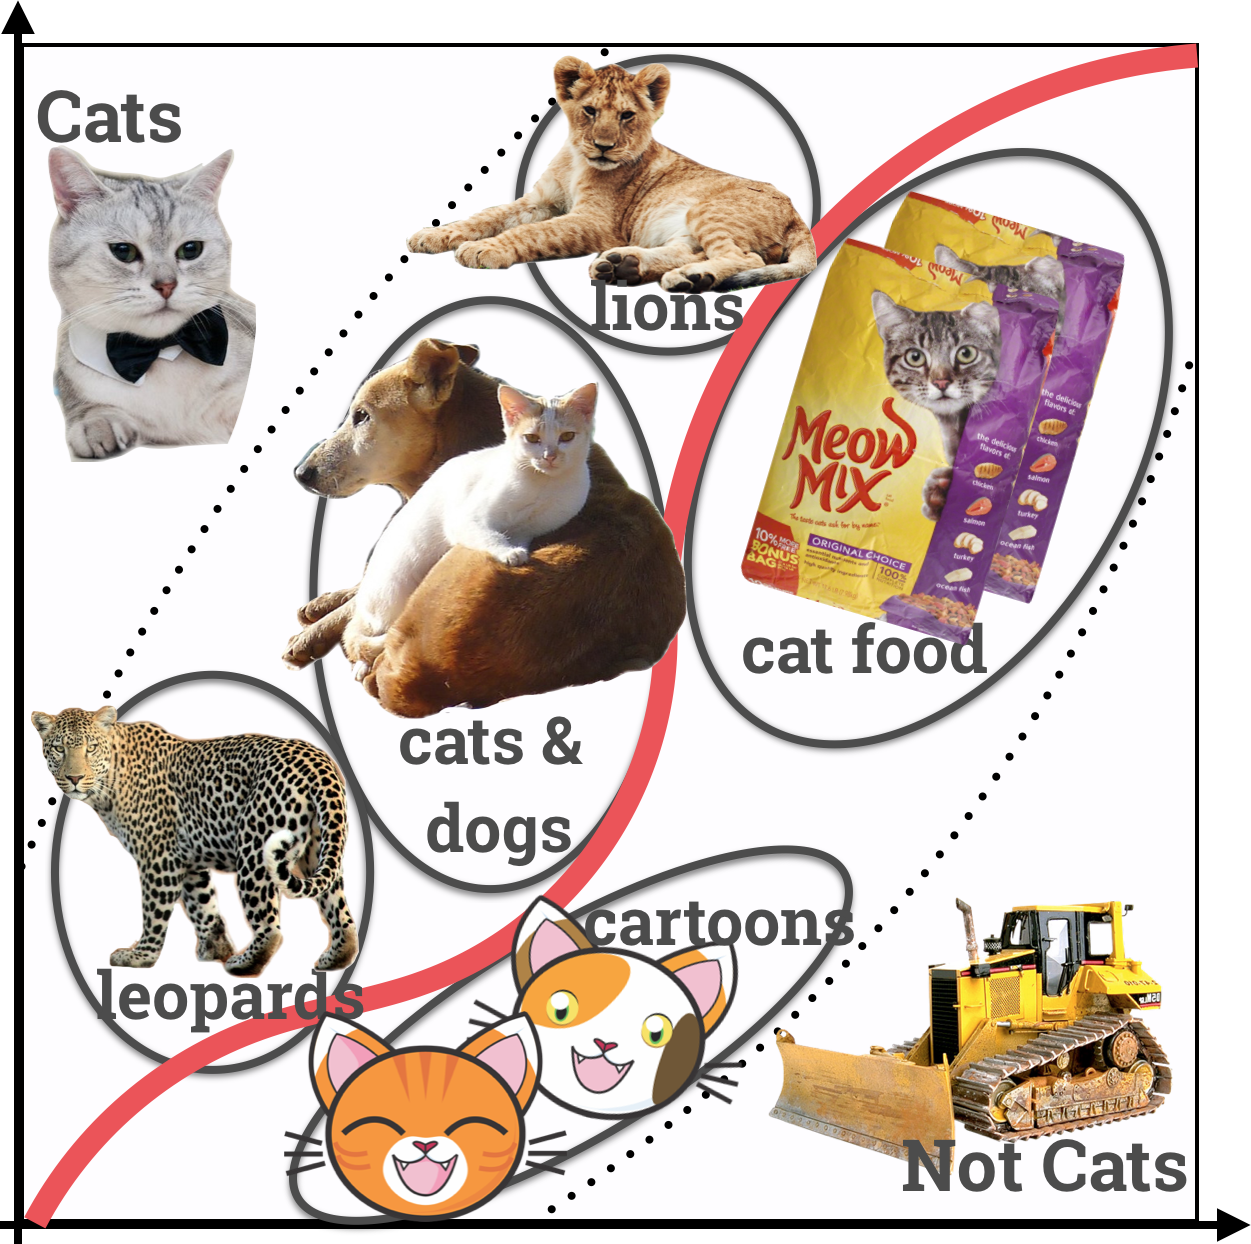
\includegraphics[width=0.45\columnwidth]{Chapters/Revolt/figures/bannerCC2.png}
	\caption[A high level view of the Revolt system.]{Revolt creates labels for unanimously labeled ``certain'' items (e.g., \emph{cats} and \emph{not cats}), and surfaces categories of ``uncertain'' items enriched with crowd feedback (e.g., \emph{cats and dogs} and \emph{cartoon cats} in the dotted middle region are annotated with crowd explanations). Rich structures allow label requesters to better understand concepts in the data and make post-hoc decisions on label boundaries (e.g., assigning \emph{cats and dogs} to the \emph{cats} label and \emph{cartoon cats} to the \emph{not cats} label) rather than providing crowd-workers with a priori label guidelines.}
	\label{fig:revolt_workflow}
\end{figure}

\section{Introduction}
From conversational assistants on mobile devices, to facial recognition on digital cameras, to document classifiers in email clients, machine learning-based systems have became ubiquitous in our daily lives. Driving these systems are machine learned models that must be trained on representative datasets labeled according to target concepts (e.g., speech labeled by their intended commands, faces labeled in images, emails labeled as spam or not spam).

Techniques for collecting labeled data include recruiting experts for manual annotation \cite{taylor2003penn}, extracting relations from readily available sources (e.g., identifying bodies of text in parallel online translations \cite{Resnik:2003:WPC:964751.964753,Chang:2012:LFT:2390665.2390698}), and automatically generating labels based on user behaviors (e.g., using dwell time to implicitly mark search result relevance \cite{agichtein2006improving}). Recently, many practitioners have also turned to crowdsourcing for creating labeled datasets at low cost \cite{Snow:2008:CFG:1613715.1613751}. Successful crowdsourced data collection typically requires practitioners to communicate their desired definition of target concepts to crowdworkers through guidelines 
explaining how instances should be labeled without leaving room for interpretation. %\saleema{Ece suggested not to use subjective in the paper. Here would be a good time to introduce the correct term, perhaps ambigous, and explain. I think the problem is in the concept definition boundary. The requester has a desired boundary that they are trying to communicate, but others may have other boundaries. Everyone can recognize a category of cartoon cats. That's not ambigious. But where you draw the boundarity is ambiguous}.  %This is redundnat so i cut it: Ideally, before enlisting the crowd, practitioners typically engage in an iterative process of generating guidelines about how crowdworkers should label items in the data. 
The guideline generation process is similar but often less rigorous than the process used by expert annotators in behavioral sciences \cite{macqueen1998codebook, weston2001analyzing} whereby experts independently examine a sample of data, generate guidelines especially around possibly ambiguous concepts discovered in the data, and then discuss and iterate over the guidelines based on feedback from others \cite{kulesza2014structured}. The guidelines are used as instructions in crowdsourced labeling tasks given to multiple crowdworkers for redundancy. Label disagreements are commonly seen as noise or failure to carefully follow the guidelines, and later corrected through simple majority voting.

%\saleema{Some redundancy between this paragraph and the last}

While traditional crowd-based labeling has produced many novel datasets used for training machine learning systems \cite{deng2009imagenet,krizhevsky2012imagenet,post2012constructing}, a common assumption in labeled data collection is that every task has one correct label which can be recovered by the consensus of the crowd \cite{bachrach2012grade}. This assumption, however, rarely holds for every item even for simple concepts (e.g., \emph{cat} vs. \emph{not cat} as illustrated in Figure~\ref{fig:revolt_workflow}) and even experts have been shown to vary their labels significantly on the exact same data due to their evolving interpretations of the target concept \cite{kulesza2014structured}. Specifying comprehensive guidelines that cover all the nuances and subtleties in a dataset would require close examination of much of the data which is typically infeasible in the crowdsourcing settings.  Crowdworkers are then often presented with incomplete guidelines and left to make their own decisions on items open to interpretation. Not only can this lead to poor quality labels and machine learning models with low accuracy, efforts to detect poor quality work (e.g.,  \cite{ipeirotis2010quality,callison2010creating,hansen2013quality}) in these cases can actually be harmful due to rejection of honest work. More fundamentally, limiting crowdworkers to providing feedback only in terms of predefined labels, failing to capture their confusions and reasoning, presents a lost opportunity to discover and capture rich structures in the data that the crowdworkers had encountered. %\saleema{This is unclear. You also say this again two paragraphs from now (and better) so I'd cut this: Aiming at discovering the structure of the data rather than only labeling it can allow for reusability of the dataset when the definitions of the target concepts evolve for the requesters or varies across different users of the dataset.} 

In this chapter, we present \emph{Revolt}, a collaborative crowdsourcing system that applies ideas from expert annotation workflows to crowdsourcing (e.g., supporting flagging of ambiguous items and discussion) for creating high quality training labels for machine learning.  Revolt enables groups of workers to collaboratively label data through three stages: \textit{Vote} (where crowdworkers label as in traditional labeling), \textit{Explain} (where crowdworkers provide justifications for their labels on conflicting items), and \textit{Categorize} (where crowdworkers review explanations from others and then tag conflicting items with terms describing the newly discovered concepts). The rich information gathered from the process can then be presented to requesters at various levels of granularity for post-hoc judgments to define the final label decision boundaries.  

Revolt requires no pre-defined label guidelines aside from the top-level concept of interest (e.g., faces, spam). As a result, this approach reverses the traditional crowdsourced labeling approach by shifting label requester efforts from guideline creation to post-hoc analysis. The rich structures provided by our approach has the additional benefit of enabling label requesters to experiment with different label decision boundaries without having to re-run label generation with the wide variety of possible label guidelines. For example, for collecting labels of images of \emph{Cats} (Figure~\ref{fig:revolt_workflow}), Revolt produces structures that group together ambiguous sub-concepts such as \emph{cartoon cats}, \emph{cat food}, \emph{leopards} and \emph{lions} along with descriptive explanations about the structures. Requesters can then review these structures and experiment with machine learning models that are trained to identify \emph{leopards} and \emph{lions} as \emph{Cats} or not. 

%\saleema{Somewhere in the paper we need to explain that here we're investigating whether Revolt produces results that contain rich enough information such that requesters could make decisions. That is, this is a necesary step in determining if our real-time collaborative aproach could be used by label requesters. We don't build a UI for label requesters to generate final labels. I'm worried about hwere this should go and how it should be carefully phrased. }

This chapter makes the following contributions:
\begin{itemize}  
\setlength\itemsep{-0.26em}
%\item A new formulation of crowdsourcing labeled data collection problem that defines the problem as a collaboration between crowds and requesters, eliminating dependency to comprehensive guidelines. \saleema{I don't think this is a contribution on its own. Are you the first to do this? I thought you mentioned in related work that there has been communication with requesters and crowds for other tasks. I'd merge this with the Revolt contribution.}   
\item A new approach to crowdsourcing label collection that employs crowds to identify uncertain aspects of the data and generate rich structures for post-hoc requester judgments, instead of trying to clearly define target concepts beforehand with comprehensive guidelines.
\item \emph{Revolt}, an implementation of our collaborative crowdsourcing approach that builds structures containing rich enough information for generating training labels for machine learning. We present both real-time and asynchronous versions of our approach. % k \saleema{Joseph, I changed this a bit to explain the real-time and async versions. Maybe adda bit to the last sentence to explain why or our main finding, that both achieve good accuracy but vary in cost.}
\item An experiment comparing Revolt to traditional crowd-based labeling on a variety of labeling tasks showing Revolt can produce high quality labels without the need for guidelines. 
\item An experiment comparing Revolt to its non-collaborative variants showing the benefits of collaboration for reducing cost and increasing quality.
%\saleema{this contradicts the abstract that says collaboration increases cost}. \joseph{the abstract is comparing Revolt to the baselines, and this is comparing Revolt to its non-collaborative variants (Solo and SoloClusterAll)}\saleema{Am I missing something? The sentence in question from the abstract is: Comparisons of real-time and asynchronous variants of \emph{Revolt} show that real-time collaboration reaches higher label accuracy in turn for an increase in monetary cost.}

%\item Findings from an informal follow up study applying Revolt to a real labeling task and presenting the resulting rich structures to a label requester for feedback. \saleema{I'm not sure we should state this as a contribution}
\end{itemize}

\section{Related Work}

\subsection{Data Labeling Techniques}

Data labeling or annotation is a common practice for many research areas. In social and behavioral sciences, researchers annotate (or code) data to build up theories about collected data, and then analyze the annotated results to discover interesting phenomena \cite{strauss1998basics}. This approach often involves multiple experts working in iterative and collaborative workflows. For example, annotators typically first examine and manually label a dataset (or subset of the dataset) independently and then compare and discuss their labels to iteratively refine a set of combined label guidelines \cite{macqueen1998codebook, weston2001analyzing}. Multiple iterations of data examination, label discussion, and guideline refinement may also occur to ensure the quality and coverage of the final guidelines. Once the guidelines stabilize, annotators can then independently label additional data accordingly to produce consistent final labels with high agreement.

Similar collaborative and iterative workflows have been reported for creating high-quality labeled datasets used in natural language processing and machine learning (e.g., \cite{marcus1993building, wiebe1999development, kulesza2014structured}). For example, Kulesza et al. \cite{kulesza2014structured} found that annotators often evolved their conceptual definition of a target concept and their corresponding labels throughout the course of observing more items in a dataset. Here, allowing annotators to create explicit structures designating ambiguous items discovered during labeling enabled them to gradually build up a better global understanding of the data and generate more consistent final labels. Wiebe et al. \cite{wiebe1999development} also proposed an iterative and collaborative workflow that relies on comparing and discussing conflicting labels amongst expert annotators to construct and refine shared labeling guidelines for producing training labels for complex datasets. 
These iterative and collaborative processes provide expert annotators systematic ways to learn about and discuss different interpretations of data during labeling. %\saleema{Joseph, which of the references in this paragraph take a collaborative approach? I think you should expand on one of them in a sentence or two. Otherwise this paragraph is just about iteration.}

While expert annotation has been used in creating labeled datasets for machine learning, this process is often too costly and time consuming to scale to the large datasets required for modern machine learning algorithms. As an example, the Penn Treebank dataset that is commonly used in natural language processing for training part-of-speech sequence labelers and syntactic parsers, was built by teams of linguists over the course of eight years \cite{taylor2003penn}. Another example from a previous work showed labeling 1,000 English sentences took four experts nine hours each to iteratively refine their guidelines by labeling items independently then discussing together \cite{wiebe1999development}. %\saleema{This wasn't a "labeling experiment" was it? I assume it was some machine learning problem that required some labeled data. Maybe something about evaluating some new algorithm with labeled data?} \joseph{the core contribution of the paper is an expert annotation workflow and a redundant label aggregation method that can produce high quality training label for machine learning models}
Many researchers and practitioners have therefore recently turned to crowdsourcing to label data for its scalability and relatively low cost \cite{deng2009imagenet,krizhevsky2012imagenet,post2012constructing}. However, despite its efficiency, researchers have also reported difficulty obtaining high quality labels using crowdsourcing \cite{alonso2013some,Demartini:2012:ZLP:2187836.2187900}. Multiple factors can contribute to poor quality labels, such as poor work from inattentive labelers, uncertainty in the task itself (resulting from poorly written guidelines or confusing interfaces), varying worker backgrounds and prior knowledge, or items that are difficult to understand by novice workers \cite{knowlton1966definition}. 

\subsection{Improving the Quality of Crowdsourced Labels}
While disagreements between expert annotators are typically resolved through discussing and refining guidelines \cite{marcus1993building}, disagreements in crowdsourcing are commonly seen as labeling errors to be corrected through majority voting over independent redundant judgments of crowdworkers \cite{kairam2016parting}. 
Methods for further improving the quality of crowdsourced labels can be mainly broken down into two camps \cite{kittur2013future}: techniques for preventing poor quality work and techniques for post-hoc detection of poor quality work. Prevention techniques include screening for crowdworkers capable of different tasks \cite{Difallah:2013:PTM:2488388.2488421,kamar2012combining}, pre-training crowdworkers \cite{doroudi2016toward}, maintaining quality while controlling for cost via dynamic task allocation \cite{Tran-Thanh:2014:BBL:2615731.2615809,bragg2013crowdsourcing}, or designing interfaces or payment structures to motivate good work \cite{mitra2015comparing,rogstadius2011assessment,hansen2013quality}. Post-hoc identification techniques include probabilistic modeling based on crowdworker agreements for weighted voting \cite{ipeirotis2010quality}, analyzing crowdworker behaviors during tasks \cite{rzeszotarski2012crowdscape}, and using additional crowdworkers to review the work of others \cite{callison2010creating,hansen2013quality}.

A common assumption in previous work is that every item has one correct label, and conflicts among crowdworkers are the result of poor quality work from novice or inattentive workers. However, constructing comprehensive and clear instructions about how to correctly label a dataset is often not possible due to the large variety of nuances and subtleties that may exist in the data, even for seemingly simple topics. For example, requesters wanting to identify \emph{cat} photos in a dataset might not be aware that the dataset also contains photos of \emph{leopards}, and/or that leopards are sometimes referred to as \emph{big cats}. As a result, crowdworkers often have to label with incomplete information. Concepts not specified in guidelines are then open to interpretation and confusion amongst crowdworkers (e.g., ``should \emph{leopards}, \emph{lion cubs}, or \emph{cartoon cats} be labeled as \emph{cats}?'' Figure~\ref{fig:revolt_workflow}), potentially leading to inconsistent labels (e.g., only some \emph{leopard} items being labeled as \emph{cats}). Methods for identifying poor work are ineffective in these cases and can be harmful to both crowdworker and requester reputations due to rejection of honest work. More fundamentally, this suggests a lost opportunity for requesters to discover interesting new concepts already identified by human computation during the labeling process since the crowdworkers are typically constrained to provide feedback in the form of predefined labels (e.g., \emph{cats} or \emph{not cats}, but not \emph{leopards}).

Even if requesters attempt to create comprehensive guidelines, they often have to review large portions of a dataset to do so which can be prohibitively expensive. Moreover, as guidelines become more complete, they can also become longer and more complicated (e.g., \cite{google} and \cite{bing}), requiring more crowdworker training or resulting in more errors. If the resulting label quality is inadequate, requesters will typically have to go through the tedious process of reviewing inconsistencies, identifying sources of confusion, updating the guidelines, and collecting entirely new labels given the updated guidelines \cite{kulesza2014structured}, potentially doubling the monetary cost of the process. 

\subsection{Harnessing the Diversity of Crowdsourcing}
Instead of treating crowdworker disagreement as noise introduced by poor work or lack of expertise, researchers have recently begun exploring methods to harness these disagreements as valuable signals. For example, researchers have found that disagreements amongst novice workers in syntactic labeling tasks often mirror disagreements amongst linguists \cite{plank2014linguistically} and are useful signals for identifying poor task designs \cite{inel2014crowdtruth}. %\saleema{Joseph, I took a pass at fixing the last bit of this paragraph. Check that it makes sense. If I'm missing something about related work, the old text is commented out below}
In another example, Kairam and Heer \cite{kairam2016parting} used label agreements to cluster crowdworkers into worker types (e.g., \emph{liberal} and \emph{conservative} labelers that identified different amount of targets in an entity extraction task). Manual analysis of these clusters were then used to improve future task designs. In contrast to this previous work, we use crowd disagreements to identify and explain ambiguous concepts in data for the purpose generating labeled data for machine learning. 

%In another example, Kairam and Heer \cite{kairam2016parting} clustered crowdworkers based on their label agreements, and manually analyzed the clusters to improve task designs through iteration. In their evaluations, clusters of crowdworkers in a named entity identification and classification task showed different characteristics, such as \emph{liberal} and \emph{conservative} workers, and also crowdworkers who interpreted the target concepts differently and labeled \emph{Botanic Gardens} as either \emph{facilities} or \emph{locations}. \saleema{Need a sentence about how our work is different from these. e.g., we use disagreements/diversity to identify and describe ambiguous concepts}

%\saleema{Joseph I revised the following paragraph. Check that it is accurate since I'm not familiar with MicroTalk}
Most closely related to our work is the MicroTalk system \cite{drapeau2016microtalk} which used crowd diversity to collect and present counterarguments to crowdworkers during labeling to improve label quality. However, this approach still assumes that a single correct label exists for every item and requires crowdworkers to pass a training stage to learn label guidelines before participating. In our work, we tackle the problem of labeling with untrained crowdworkers under the assumption that a single correct label might not exist for every item. Diversity in interpretation is then used to create rich structures of uncertain items for post-hoc label decisions, avoiding the burden of creating comprehensive guidelines beforehand and pre-training crowdworkers. We compare our approach to a condition inspired by MicroTalk called \emph{Revote}, showing that Revolt can produce training labels with higher accuracy under the scenario where comprehensive guidelines are not available.
%asked crowdworkers to justify their labels with short explanations, and present these arguments to future workers who labeled the same items differently. They found that some crowdworkers who failed to identify the correct label was able to reconsider their labels after seeing the counterarguments, increasing the overall labeling accuracy.
%However, the system required pre-constructed guidelines and pre-trained crowdworkers, and still assumed a single correct answer for all items.

%\ece{We need a stronger statement here to seperate our work from drapeau2016microtalk. Do they study the same problem we do, or do they still assume a single correct answer exists for each task and conflicts occur due to worker errors? If it is the second one, I'd start differentiating our work by saying that we study a different problem and do not make the assumptions they are making. }

%\saleema{I cut what was here because it was redundant}

%\ece{I found the following paragraph redundant given the intro. Only keeping the first sentence would suffice.} \joseph{i commented out the second sentence, its probably too specific here}
%In this work, rather than leverage crowdworker diversity for improving task designs to better generate single correct answers, we exploit crowdsourcing mechanisms to capture disagreements and root causes of disagreements as they occur, and allow crowdworkers to resolve these conflicts by creating rich structures through collaboration. 
%More specifically, we design workflows for generating high quality labels for training data by grouping crowdworkers into small ad-hoc teams, allowing them to exchange individual interpretations and report back information learned via categories of ambiguous items. These structures can then be presented to label requesters to make the final decisions without changing the tasks or hiring more crowdworkers (e.g., freely assign the \emph{leopard} category with the \emph{cat} or \emph{not cat} labels).



%\joseph{i did another pass}
%\saleema{This still sounds like a post-hoc analysis type of thing which still sounds similar to previous work. Maybe clarify what previous work used the disagreement driven structures for. Did they use it for ML? What about using it for ML makes it different? }

\subsection{Structuring Unlabeled Data with the Crowd}
Crowd structuring refers to tasks that make use of crowdsourcing for organizing information without predefined target concepts. For example, categorizing \cite{alloy,crowdsynth} or create taxonomies \cite{cascade} for a set of documents. In contrast, our work focuses on the task of \emph{crowd labeling} which is the task of assigning predefined target concepts to each item in a dataset. In our approach, crowdworkers perform structuring within a labeling task, and only to resolve different interpretations of the same items for post-hoc requester review. Past work in crowd structuring also typically involves multiple stages completed by different crowdworkers working independently, while we took a different approach by utilizing real-time crowdsourcing to maintain a shared global structure synchronized across groups of crowdworkers working collaboratively. 

%These past work on crowd structuring focused on the task of discovering topical categories in a set of textual data, while we focused on creating structures within a labeling task for resolving different interpretations of the same items from different crowdworkers. Comparing to previous work in crowd clustering, we took a simpler approach by maintaining a shared global structure synchronized in real-time across crowdworkers labeling different partitions of the dataset. In addition, before attempting to categorize items, crowdworkers in our system had already gained a rich understanding of the dataset by working on the same items in two previous stages. 

%Failure to do so could lead to categories that are overly abstract or overly fine-grained \cite{alloy}. Past work has taken different approaches to tackle this problem, such as presenting multiple items to each crowdworker \cite{crowdsynth}, organizing overlapping categories into ontological structures \cite{cascade}, or using a sampling and searching mechanism that allowed crowdworkers to actively explore the dataset for context \cite{alloy}. Past work typically involves a multistage pipeline where some crowdworkers first create categories based on different subsets of the dataset, and then presenting the crowd categories to other crowdworkers for aggregation and refinement.

%\ece{Explicitly say why previous work on crowd structuring is not the answer to our problems.}


\subsection{Real-time Crowdsourcing}
Real-time crowdsourcing has been employed for a variety of purposes including minimizing reaction time in crowd-powered user interfaces \cite{bigham2010vizwiz,Bernstein:2011:CTS:2047196.2047201,Burton:2012:CSF:2384916.2384941,laput2015zensors,lasecki2013chorus}, increasing the speed of data collection \cite{lasecki2014glance,Krishna:2016:EEE:2858036.2858115}, and improving data quality by incorporating expert interventions to guide novice workers \cite{chan2016improving,dow2012shepherding,kim2014ensemble}.
In our work, we use real-time crowd-based collaboration to improve the quality of labeled data without expert intervention. Workers engage in real-time collaboration to build rich structures of data that incorporate different crowdworker perspectives and can be analyzed post-hoc. Moreover, while most previous real-time systems employ multiple crowdworkers in a single shared workspace, our approach dynamically coordinates crowdworkers to move synchronously between stages of different subtasks. Within each stage, crowdworkers make independent judgments to be revealed to others in subsequent stages. In this way, our approach still benefits from common crowdsourcing mechanisms of verification through redundant independent judgments, but can also capture and utilize diverse crowd perspectives through collaboration. 


\section{System Design}

\begin{figure}[ht]
	\centering
	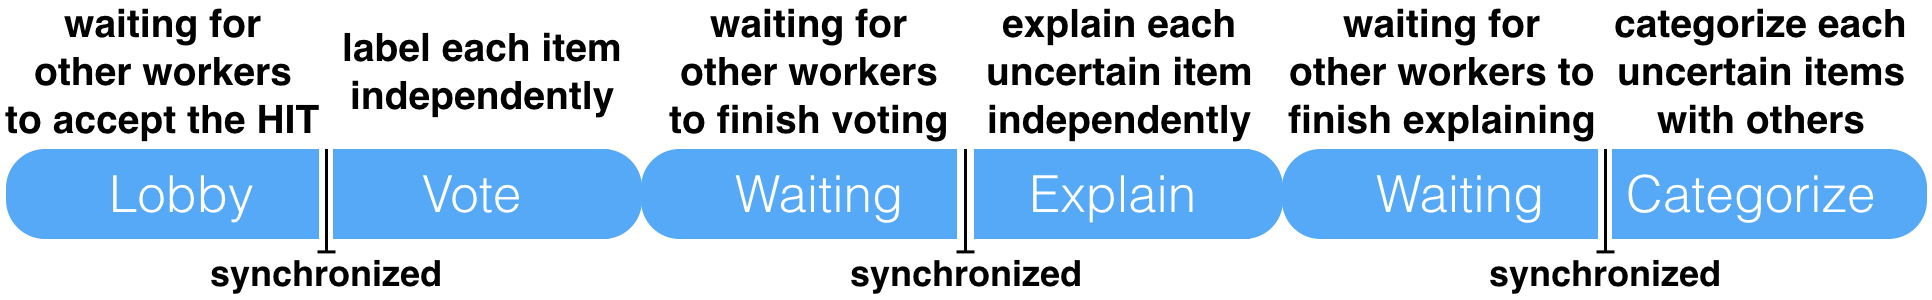
\includegraphics[width=0.9\columnwidth]{Chapters/Revolt/figures/overview3.png}
	\caption[Overview of Revolt stages.]{
	Overview of Revolt Stages: Synchronized stages requires all crowdworkers in the group to complete in order to move on. 
	}
	\label{fig:overview}
\end{figure}

In this section, we describe Revolt, a collaborative crowdsourcing system for generating labeled datasets for machine learning. Throughout this section, we use the task of labeling images as being about ``\emph{Cats}'' or ``\emph{Not Cats}'' as a running example (Figure~\ref{fig:revolt_workflow}).

At a high level, Revolt divides a dataset into multiple batches and then coordinates crowdworkers to create labels for \emph{certain} items (items receiving unanimous labels from multiple crowdworkers) in each batch and identify \emph{uncertain} items (items receiving conflicting labels) for further explanation and processing. In the synchronized version (Revolt), the system coordinates small teams of three crowdworkers through three synchronized stages: Vote, Explain, and then Categorize (see Figure~\ref{fig:overview}). In the asynchronized version (RevoltAsync), the system elicits different crowdworkers to work independently in the Vote and Explain stages, maintaining the same redundant judgement of three crowdworkers per item while eliminating the cost of coordinating crowdworkers in real-time. After collecting crowd judgments and explanations across all batches, both systems algorithmically produce structures (groups of semantically related items) at various levels of granularity for review by label requesters to determine final label decision boundaries (e.g., assigning the ``\emph{Cartoon Cats}'' category as ``\emph{Not Cats}'') before training a machine learning model. To minimize redundant information, the rest of this section describes Revolt in the context of the synchronized version. We then describe the differences of the RevoltAsync condition.


\subsection{The Vote Stage}

\begin{figure}[ht]
	\centering
	\frame{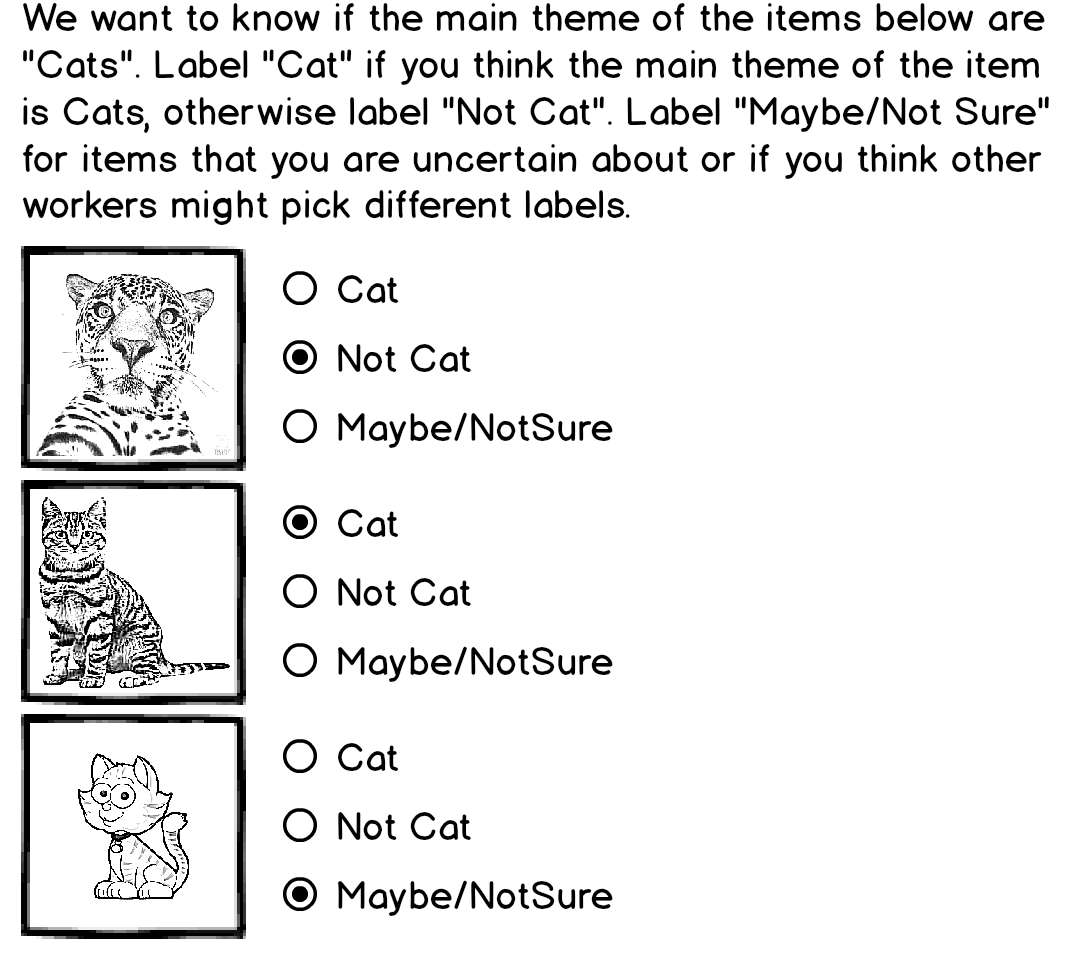
\includegraphics[width=0.6\columnwidth]{Chapters/Revolt/figures/vote.png}}
	\caption[HIT interface for the Vote Stage of Revolt]{
	Human Intelligence Task (HIT) interface for the Vote Stage. In addition to the predefined labels, crowdworkers can also select \emph{Maybe/NotSure} when they were uncertain about the item. 
	}
	\label{fig:vote}
\end{figure}

Revolt initially keeps crowdworkers in a lobby until enough crowdworkers have accepted the task and can begin as a group (Figure~\ref{fig:overview}). The Vote stage then begins by collecting independent label judgments from multiple crowdworkers using an interface similar to that used in traditional crowdsourced labeling (see Figure~\ref{fig:vote}). In addition to showing predefined labels as options at this stage (e.g., ``\emph{Cat}'' or ``\emph{Not Cat}''), we also include a ``\emph{Maybe/NotSure}'' option to ensure crowdworkers are not forced to make arbitrary decisions for uncertain items that should instead be explained further in subsequent stages. Through task instructions, crowdworkers at this stage are informed that others in the same group are also labeling the same items at the same time, and that they will be asked to compare their labels in subsequent stages. By allowing workers to express their uncertainty in the data and provide feedback in subsequent stages, Revolt avoids unfairly rejecting honest work \cite{mcinnis2016taking}.

Before Revolt can proceed to the next stage, all crowdworkers in a group must finish labeling all items in their batch. Crowdworkers who finish early are put into a waiting area where they can see in real-time how many crowdworkers in their group are still labeling items. Once the group is ready to continue, desktop and audio notifications are sent to all crowdworkers in case any stepped away while waiting. Once all labels are received, \emph{certain} items are assigned their final labels as usual, and \emph{uncertain} items (including items that received ``\emph{Maybe/NotSure}'' labels) proceed to the Explain stage.


\subsection{The Explain Stage}

\begin{figure}[ht]
	\centering
	\frame{\includegraphics[width=0.6\columnwidth]{Chapters/Revolt/figures/explain.png}}
	\caption[HIT interface for the Explain Stage of Revolt]{
	Human Intelligence Task (HIT) interface for the Explain Stage. Crowdworkers enter a short description for each item that was labeled differently in the Vote Stage. They were informed that disagreement occurred, but not the distribution of different labels used. 
	}
	\label{fig:explain}
\end{figure}


In the Explain stage, crowdworkers are asked to provide short explanations about their labels for items flagged as \emph{uncertain} in the previous stage. Instructions informed each crowdworker that others in the group disagreed on the labels for these items and therefore their task was to describe their rationale for each label to the rest of the group (see Figure~\ref{fig:explain}). 

Note that early prototypes of our system also revealed the individual votes from other crowdworkers on each item at this stage. However, pilot experiments showed that this resulted in less descriptive explanations that were more focused on reacting to other crowdworkers. For example, people who picked the majority vote labels often simply reaffirmed or expressed confidence in their original label (e.g., ``\emph{nothing says to me that this is a cat}'') , whereas people who were in the minority often just yielded to the majority (e.g., ``\emph{this could be a cat, i might have messed this one up}''). Instead, hiding the labels and only stating that a disagreement had occurred resulted in more conceptual explanations helpful for the following stage (e.g., ``\emph{This is not a cat, but rather one of the big felines. Leopard or Cheetah I think.}'' and ``\emph{Although leopards are not domesticated, they are still cats.}''). As in the Vote Stage, crowdworkers who finished early were placed in a waiting area before they could move on together.


\subsection{The Categorize Stage}

\begin{figure}[ht]
	\centering
	\frame{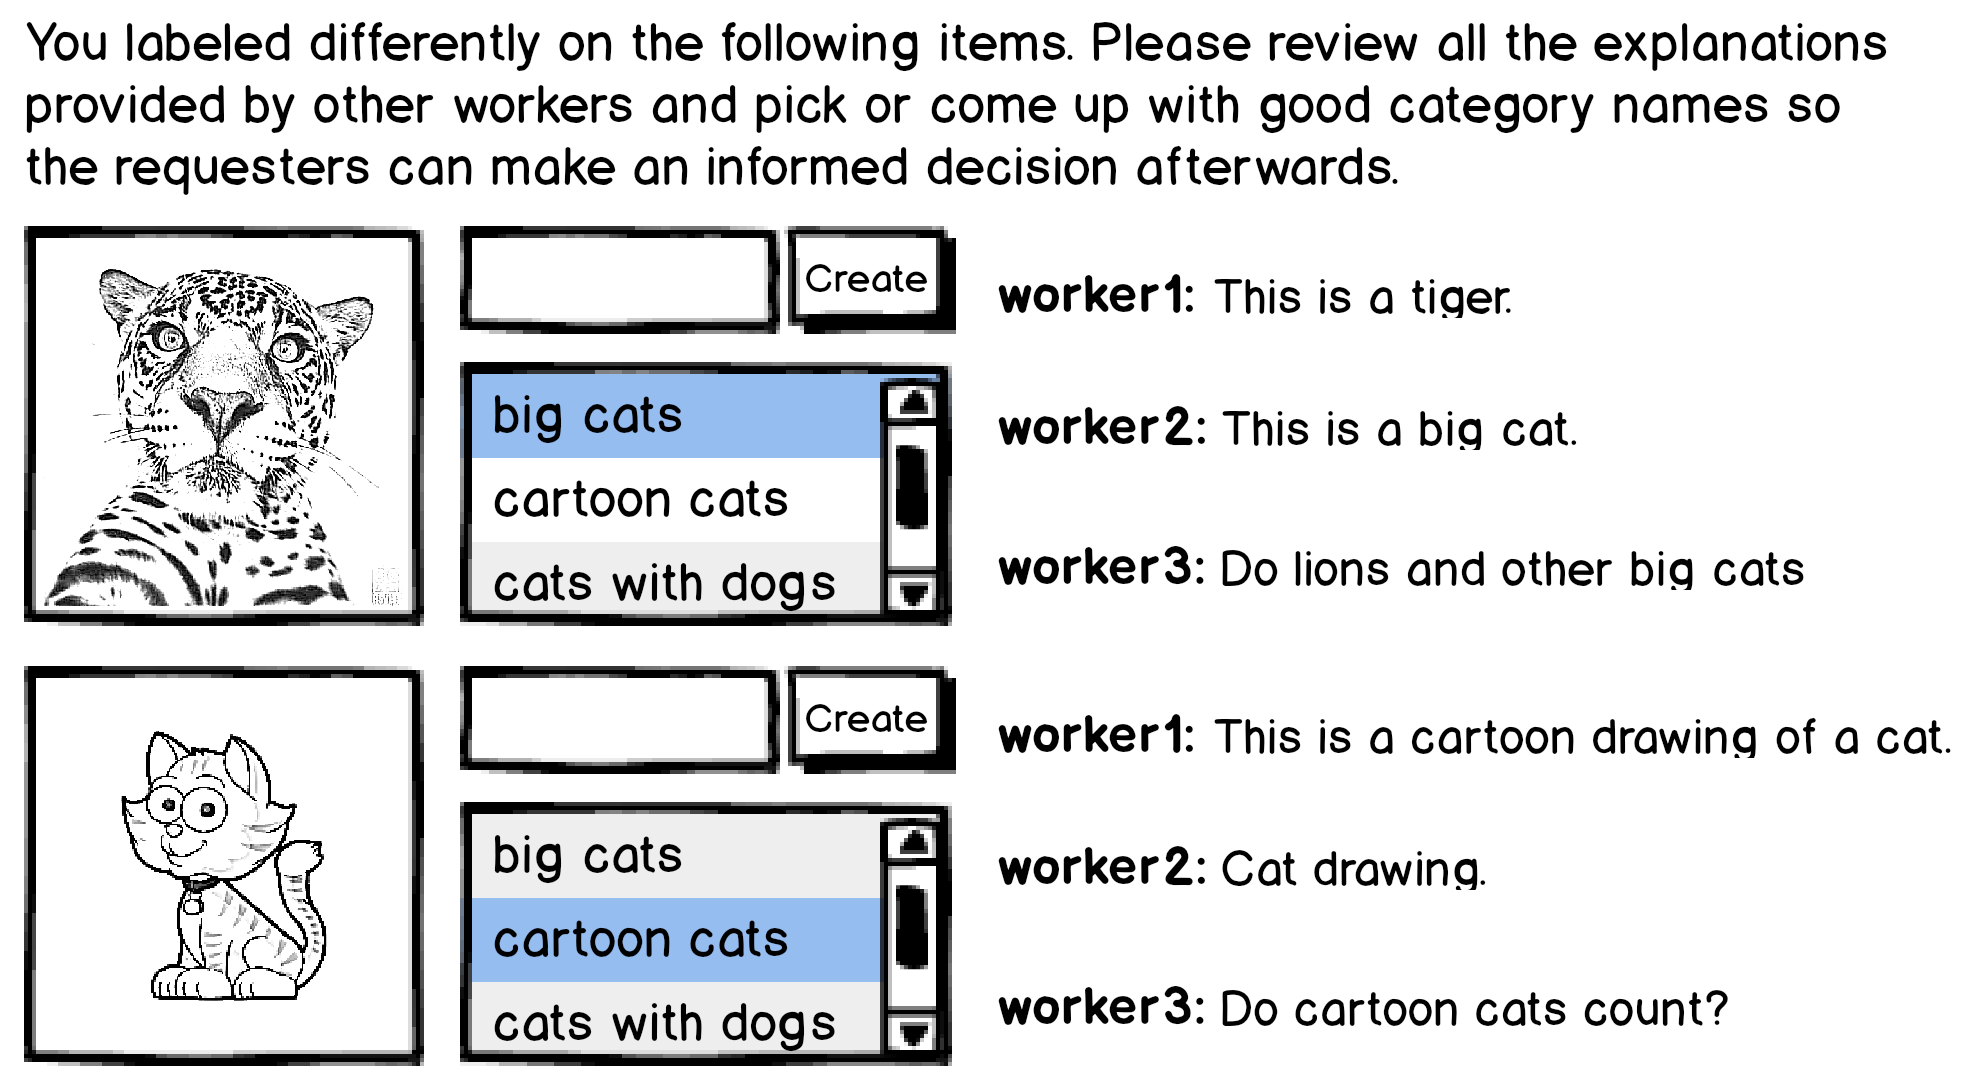
\includegraphics[width=0.6\columnwidth]{Chapters/Revolt/figures/categorize.png}}
	\caption[HIT interface for the Categorize Stage of Revolt]{
	Human Intelligence Task (HIT) interface for the Categorize Stage. Crowdworkers select or create categories for items that were labeled differently in the Vote Stage, based on explanations from all three crowdworkers in the same group. 
	}
	\label{fig:categorize}
\end{figure}


In the Categorize stage, crowdworkers were tasked with grouping uncertain items into categories based on their explanations. In this stage, we present the same uncertain items to each crowdworker again, but this time also reveal the explanations from others in the group (Figure~\ref{fig:categorize}). Crowdworkers were then instructed to categorize each item based on its explanations. Categories could either be selected from a list of existing categories presented next to each item or added manually via a text input field. Whenever a new category was added by a crowdworker, each list of categories was synchronized and dynamically updated across all items within the current group, and also across groups working on different parts of the dataset. To encourage category reuse and reduce redundancy we also implemented two mechanisms: First, the text field for creating categories also acts as a quick filter of the existing categories so that crowdworkers may more easily see and select an existing category rather than create a new one when appropriate. Second, the list of existing categories is sorted by the number of crowdworkers (across all batches of the same dataset) that have used each category, a similar strategy to that used to filter out low quality crowd categories in \cite{cascade,chilton2014frenzy}. % Here we used simple realtime crowdsourcing techniques to categorize the uncertain data, however, many more sophisticated (yet often more costly) none realtime solutions also exist in previous work. \ece{say a bit more here. How do these approaches look like? Do they depend on crowdsourcing or some automated approaches?} We will discuss the limitations of our approach in the Discussion Section. % im cutting this for space...
After assigning categories, crowdworkers could submit their HITs independently without waiting for others to complete.  
 
%\saleema{Explain the problem first. E.g., "In pilot experiments we noticed that naively updating the list or sorting the list in some way, resulted in too many redundant or synonymous categories". Then describe your solution: Two simple mechanisms were implemented to reduce redundant or synonymous categories. First, as the crowdworkers typed in the text input box for creating a new category, the category list will update and show only category names that contain the user input. Second, the list of existing category is sorted by the number of crowdworkers that have used each category, a similar strategy that was also used in past research for filtering out low quality crowd categories \cite{cascade}.}

\subsection{Post Processing of Crowdworker Responses}
%\ece{This section needs a bit more work. Here are my main issues: (1) We discuss two different ways of creating categories: simple majority voting and clustering. Which one do we do? If we do clustering at the end, why even talk about majority voting? I thought we were using majority voting categories as constraints in clustering. If so, we should say so. (2)As far as I understand, the clustering step works on explanations. if you are applying clustering at the end, how do you use the categorize stage after all? Is the categorize step unnecessary if you are using clustering? It is unclear how you are jointly using the outputs of explain and categorize steps in clustering. }
After crowdworkers in all groups have gone through all three stages, Revolt collects the crowd feedback for all batches. Revolt assigns labels to \emph{certain} items directly, and then creates structures of \emph{uncertain} items by applying simple majority voting on the category names suggested by crowdworkers for each item. In cases where all crowdworkers suggested a different category, a random crowdworker's category is used as the final category. At this point, structures can be presented to label requesters for review and to make final label decisions. For example, after reviewing structures, a label requester may decide that \emph{leopards} and \emph{lions} should be considered \emph{Cats} while \emph{cartoon cats} and \emph{cat food} should be considered \emph{Not Cats}. In this way, label assignments can be applied to the data in each category prior to training a machine learning system.


Revolt can also expand the crowd-generated categories to different numbers of clusters, supporting inspection at different levels of granularity. To do this, Revolt performs a hierarchical clustering method that uses the crowd categories as connectivity constraints. 
%\saleema{The previous sentence suggests that Revolt is an incomplete system because you say that it relies in input requesters to do the final step. You have to be very careful in how you phrase this. I'd simply say that at this point requesters can view categories to make decisions. To better support the requester, Revolt can also perform a post processing step to break down or build up categories at different levels of granularity etc...}
%Once clusters are created, the requester input is used to assign clusters to labels 
This post-processing approach works as follows:
First, a term frequency-inverse document frequency (TF-IDF) vector is used to represent each uncertain item where each dimension is the count of a term in its explanations divided by the number of uncertain items with the same term mentioned their explanations. Then, hierarchical clustering with cosine similarity is applied. That is, initially, each item is treated as a cluster by itself. Clusters are then iteratively merged with the most similar clusters, prioritizing clusters with items in the same crowd category, until all items are in the same cluster. 

Generating clusters at various levels of granularity allows label requesters to adjust the amount of effort they are willing to spend in making labeling decisions, allowing them to manage the trade-off between effort and accuracy. For example, labeling low level clusters allows for more expressive label decision boundaries, but at the cost of reviewing more clusters. 



% \saleema{This section needs work. 1) Do you need to talk about how to collect all items together from different batches distributed across different groups of workers? If so this should go here. 2) Then talk about the majority voting for categorization. Is it possible for requesters to look at these results directly, without clustering? If so, then describe how the categories can be presented to requesters for assignment. If your system relies on clustering to produce the groups that requesters should review then explain that first and give more details about the clustering than you have below}

% \saleema{Original text: For example, assigning the label \emph{cat} to all uncertain items in the category \emph{leopards}. In addition, the system also used the crowd categories as clustering constraints and run bottom-up clustering of the uncertain items using TF-IDF weighted cosine similarity of the explanations. This way the requesters can freely choose the number of categories they want to label as a trade-off between the amount of post-hoc requester efforts and the accuracy of the final labels. For example, in an extreme case, the requesters can re-label all uncertain items to gain higher labeling accuracy. In this study, we assume the requesters are capable of choosing the best label for each category that increases the accuracy of the final labels the most. We will discuss this further in the Evaluation and Discussion and Future Work Sections.}

\subsection{RevoltAsync}
RevoltAsync removes the real-time nature of Revolt as follows: One set of crowdworkers label items independently in the Vote stage. RevoltAsync then still uses the results of three crowdworkers per item to identify uncertain items. Uncertain items are then posted to the crowdsourcing market again for a different set of crowdworkers to explain the labels. That is, in RevoltAsync's Explain stage, crowdworkers are presented with an item and a label given by another crowdworker and then asked to justify that label given the knowledge that there were discrepancies between how people voted on this item.

RevoltAsync does not include a Categorize stage, which would require synchronization. Instead it uses the explanations collected at the Explain stage directly for clustering during post-processing. Clustering of explanations is still performed using hierarchical clustering, to produce structures at different levels of granularity, but without connectivity constraints based on the crowd categories provided by the Categorize Stage.



\section{Evaluation}

In this section, we describe experiments we conducted to investigate the cost-benefit trade-off of Revolt compared to the traditional crowdsourcing approach for collecting labeled training data. We also examined several variants of Revolt to better understand the benefits of different components of the Revolt system and workflow. 
%Since the design space of collaborative labeling workflows is not limited to the one described in the earlier section, we also experimented with  variants of Revolt. \saleema{Rephrase that last sentence. Saying that Revolt is just one instance of a design space minimizes the contribution. In fact you tried many different versions of Revolt we got to something that worked well. Plus this statement is true for all UIs. Just explain why you wanted to try async and other variants, e.g., to examine the benefits of real-time over...}

To compare these workflows, we ran each condition on a variety of datasets and measured the accuracy of the resulting labels with respect to requester effort and crowdsourcing cost. To prevent learning effects, we do not reuse crowdworkers across conditions for the same dataset, and randomize posting order of condition and dataset combinations so that crowdworkers subscribed to postings from our requester account using third party services\footnote{http://www.turkalert.com/} were distributed across conditions.

\subsection{Baselines and Conditions}

Our conditions include Revolt, RevoltAsync, three variants, and two baselines representing traditional labeling approaches:

\begin{itemize}
    \setlength\itemsep{-0.2em}
	\item \emph{NoGuidelines}. A baseline condition where crowdworkers label items without guidelines. This condition should be considered a lower bound baseline, since in most real world scenarios requesters are likely to have some knowledge of the data or desired labels to create some initial guidelines. 
	\item \emph{WithGuidelines}. A baseline condition where crowdworkers label items according to provided guidelines. For this condition we endeavored to create comprehensive guidelines that left no room for subjective assessment as explained in the next Datasets and Guidelines section. Since creating comprehensive guidelines is often infeasible in realistic machine learning tasks, the results from this baseline should be considered an upper bound for what can be achieved with traditional crowdsourced labeling.
	\item \emph{Revolt}. Our proposed Vote-Explain-Categorize workflow with synchronized real-time collaboration.
	\item \emph{RevoltAsync}. Our Revolt variant with asynchronous collaboration mechanisms.
	\item \emph{Revote}. A Revolt variant with similar strategies used in \cite{drapeau2016microtalk} wherein crowdworkers re-label uncertain items after considering each others' explanations instead of categorizing them for post-hoc requester review. This variant replaces Revolt's Categorize stage with a Revote stage (without the \emph{maybe} option) and uses simple majority voting to assign final labels to all items.
	\item \emph{Solo}. A Revolt variant with no collaboration. In this condition, each crowdworker labels and explains their labels for all items independently. The system still computes uncertain items from three redundant labels and clusters uncertain items using their explanations.
	\item \emph{SoloClusterAll}. A variant of \emph{Solo} where the system clusters all items based on their explanations. Note that clustering all items (certain and uncertain) is only possible in the \emph{Solo} variants where explanations were collected on all items. This approach creates categories for certain items as well as uncertain, requiring requester review of even items that reached consensus through crowd labeling.  
\end{itemize}

Note that no post-hoc requester effort is required in the NoGuidelines, WithGuidelines and Revote conditions and only the WithGuidelines baseline requires requesters to create guidelines prior to crowd labeling. We implemented the Revolt, Revote, Solo, and SoloClusterAll conditions using the TurkServer library \cite{mao12:turkserver}, which provided the infrastructure for recruiting and coordinating crowdworkers in real-time. Labels for the RevoltAsync, NoGuidelines, and WithGuidelines conditions were collected through the Mechanical Turk form builder feature on the requester interface. %\saleema{Mechanical Turks Form builder features?}


%\ece{I think this is out of place here. We never described how we use the categories to constrain the hierarchical clustering approach. Also this explanation is not enough, why we are doing this, why his helps.}
%For conditions that does not perform the realtime collaborative Categorize Stage, we use the clustering method described in the previous section to generate clusters at various granularity for post-hoc requester judgements. 
%\saleema{This is unclear. You do perform clustering on Revolt results whihc does have a Cateogrize stage. You also mention clustering in all the conditions so this is somewhat redudnent. If you want to mention clustering in the conditions, explain that you can produce clustering at various levels of granularity there.}

%\saleema{You also need a bit about how you implemented these conditions. Hee or in a new subsection on implementation. You should mention that Revolt was built over turkserver etc. Whereas the other condiitons were run over Mturk forms. This will be important when you get to cost and how you can't really compare these effectively.}


%\saleema{This section is super hard to follow and needs restructuring. Here's what I'd suggest: 1) In the intro paragraph to this section, describe the goal of our evaluation at a super high level which was to evaluate Revolt in terms of the cost benefit tradeoff compared to the traditional technique for generating labels. We also experiment with some variants of Revolt including [something about c3] and asychrnous variants to investigate the benefits of real-time collaboration. Then say, to compare these different workflows, we run each workflow on a variety of datasets and measure label accuracy and cost. 2) Put the Conditions subsection first. Make this mostly a bunch of bullet points briefly describing each of the conditionsn. 3) Put the Datasets next. 4) Then the Evaluation Metrics. This section should talk both about measuring accuracy and measuring cost. Alternatively, you can talk about how you measure accuracy in the Accuracy results section.}


%\joseph{move from results}
%In the first variant, we used the same workflow of Revolt with only one crowdworkers in each group, and increase the number of total groups so that all items are still labeled by three crowdworkers. Under this condition, crowdworkers can immediately move to further stages without waiting for other crowdworkers to finish the current stage. However, since crowdworkers are working independently, the system can not identify which items are uncertain in the Explain Stage, so the crowdworkers were asked to enter explanations for all items they have labeled. We also removed the Categorize Stage that is driven by a shared list of categories synchronized in real-time. We tested two conditions with this variants. In the Solo condition, the system identified the uncertain items after crowdworkers finished labeling and explaining all items, and create clusters of 




\subsection{Datasets and Guidelines}
% For generating each gold-standard label sets, we went through each item in the datasets in two passes, writing down notes and categories next to the items that can be open to interpretation in the first pass, and creating the final labels and write down labeling guidelines in the second pass.  These guidelines are likely to be unrealistically comprehensive comparing to guidelines used in most crowdsourcing labeling tasks, but we wanted to see how Revolt performs comparing to this upper bound condition.}

%\saleema{I took a pass at this section, but it might still be a bit confusing...}

We evaluated each of our conditions with eight tasks made up of different data types (images and webpages) and sizes (around 100 and 600 items, respectively). All of our datasets were obtained from the publicly available ImageNet \cite{deng2009imagenet} or Open Directory Project\footnote{https://www.dmoz.org/} databases, both commonly used for machine learning research. 

Each labeling task asked crowdworkers to label each item in a dataset as belonging or not belonging to a given concept. We used target concepts of \emph{Cars} and \emph{Cats} for our image datasets and \emph{Travel} and \emph{Gardening} for our webpage datasets to show that interpretations can vary for even seemingly simple and generally familiar concepts (Table~\ref{tab:accuracy}). For our \emph{Cars} and \emph{Cats} image datsets, we collected images from ImageNet \cite{deng2009imagenet} by first collecting all images that corresponded to WordNet \cite{miller1995wordnet} concepts containing the keyword ``car'' or ``cat'', and then sub-sampling the set down to approximately 600 images per dataset while ensuring no sub-concept (such as \emph{sports car} or \emph{cable car}) was overrepresented (>10\%) in the final set. We obtained our \emph{Travel} and \emph{Gardening} webpage datasets from \cite{kulesza2014structured} which has approximately 100 webpages for each concept obtained from the Open Directory Project by selecting half from each category, ``travel'' or ``gardening'', and then selecting the remainder randomly from the database.

For each dataset, we generated two sets of gold-standard labels and corresponding guidelines (making eith datasets total) representing two different interpretations of the same concept in the following way: 
%For each dataset, each author generated a set of gold-standard labels and corresponding guidelines according to their own interpretation of the target concept, acting like a label requester defining their desire label boundaries for their task.
Independently, each author first manually labeled the datasets using a structured labeling process \cite{kulesza2014structured} where they would categorize items as they examined them and then assign final labels at the end. This resulted in gold-standard labels and guidelines describing those labels (defined by rules each author would write down describing their categorizations and final label assignments) for that dataset. These guidelines can be considered comprehensive given that each item was examined during labeling. In realistic tasks with potentially large or complex datasets, it is often infeasible for label requesters to manually examine each item in order to create a set of guidelines (instead they typically examine a subset). Table~\ref{tab:accuracy} summarizes our datasets. To give some insights into the level of ambiguity that existed in each datasets, we report the proportions of items that received conflicting labels under the NoGuidelines conditions as $\mu$. The average proportion of items being assigned the positive labels in each dataset is 0.41 ($\sigma=0.12$).  
%\saleema{I took out this bit because it was confusing at this point since we haven't mentioned gold-standard labels yet...see if you can put it back somewhere that makes sense: This resulted in 39\% to 56\% of the items being assigned the positive labels in the gold-standard.} // moved from previous paragraph

%For each dataset, each author generated a set of gold-standard labels and corresponding guidelines according to their own interpretation of the target concept, acting like a label requester defining their desire label boundaries for their task.
%Independently, the authors first manually labeled the datasets using a structured labeling process \cite{kulesza2014structured} where they would categorize items as they examined them and then assign final labels at the end. This resulted in gold-standard labels and guidelines describing those labels (defined by rules each author would write down describing their categorizations and final label assignments) for that dataset. These guidelines can be considered fairly comprehensive given that each item was examined during labeling. In realistic tasks with potentially large or complex datasets, it is often infeasible for label requesters to manually examine each item in order to create a set of guidelines (instead they typically examine a subset). Table~\ref{tab:accuracy} summarizes our datasets.

%, and to give some intuition about the amount of uncertainty of each dataset, we also report the proportion of uncertain items $\mu$ that received conflicting labels when crowdworkers were labeling with the NoGuidelines condition. \saleema{What happened to Table 2? I don't see it. You should also explain why we care about the proportion of uncertain items. Are you going to do an analysis of results based on uncertainty or at least a discussion about how the proportion of uncertainty impacts things? I don't think you should get rid of this, but just be sure to disucss it later}

% \saleema{We should add this, but it might be better in the results section: . }


%For each dataset, we generated two sets of gold-standard labels (e.g., \emph{cats} or \emph{not cats}) and guidelines by labeling every item. To ensure the quality and consistency the gold-standard labels, we used a structured labeling process similar to \cite{kulesza2014structured}, examining the items in two passes, writing down notes and categories next to the items that can be interpreted differently, and creating final labels and guidelines in the second pass. 




%\subsubsection{Images from ImageNet}
%The ImageNet database consists of around 14 million images\footnote[1]{as of September of 2016} labeled with concepts from the WordNet ontology (also called \emph{synonym set} or \emph{synset} for short) \cite{deng2009imagenet}. Each of these concepts consists of a short definition and a set of synonymous phrases that refer to the concept \cite{miller1995wordnet}.
%The WordNet database consists of around 120 thousands synsets \footnote[1]{} organized in ontological structures \cite{miller1995wordnet}.
%For example, the synset \emph{\{dog, domestic dog\}} has the hypernym of \emph{\{canine, candid\}}, which in turn has the hypernym of \emph{\{carnivore\}}.
%However, this can sometimes be problematic in practice due to the ambiguity of natural language.
%For example, searching WordNet with the term "dog" leads to \emph{\{dog, domestic dog\}}, but also \emph{\{frank, hotdog, dog\}}, \emph{\{dog (informal term for a man)\}}, and five other concepts.
%To select subsets of images for labeling, we randomly selected two sets of around 600 images that correspond to WordNet synsets containing the words "cat" or "car", respectively. Since the images were already labeled, one obvious approach was to create gold-standard labels and guidelines at the synset level. However, the ImageNet dataset was also labeled by crowdworkers, and we wanted to err on the side of caution. We therefore relabeled the individual images using the approach described in the previous subsection, ans was able to correct a small number of errors.
%(For example, one photo of a house cat sitting on an image scanner was labeled with the synset \emph{\{CAT scan, CT scan\}}.)

%\subsubsection{Webpages from the Open Directory Project}

%\joseph{briefly describe the Open Directory Project, the criteria used in the structured labeling paper to select the webpages, give an example of why some webpages might be ambiguous, and point readers to the structured labeling paper for detail} 



%\saleema{I don't think this formalism is adding anything. Much of this formalism is also just talking about the workflow which you already described in the Revolt section. For example, you should have already explained in the Revolt section how you use majority voting for assigning category labels to items. So can we simplify this and just explain our technique verbally. Something like "Revolt produces labels on certain items and categorizes uncertain items into groups (you should have already explained the clustering in the Revolt section) that are intended to be reviewed by requesters to make final labeling decisions. We simulate requester assignments to categories by [describe assigning to majority class label]. Explain that this is a reasonable simulation because at the very least, without any UI support for generating group summaries or anything, you would expect that the requester could view one or two items in a category in order to make an assignment decision. Then you can say something about the likelihood of picking an item from the majority in the group. Once you've assigned each item to the positive/negative class using the direct results for certain items and the simulated category assignments you can just measure accuracy against the ground truth as normal. You should also mention here that because your system can produce groups at various levels of granularity using the bottom up clustering you described earlier, you can measure accuracy and cost at each level of granularity.}



\begin{table}[ht]
\centering
\footnotesize


\begin{tabular}{r r r r | r r r | r r r r r}

\hline
% & & & C1 & C2 & C3 & C5 & C8 & C9 & &  \\
Dataset & Type & N & $\mu$ & NoGdlns. & W/Gdlns. & Revote & Revolt & Solo & SoloAll & RVAsync & \#Cats \\
\hline
Cars1   & img & 612 & .27 & .843 & .887 & .820 & \textbf{.904} & .863 & .884 & .882 & 32 \\
Cars2   & img & 612 & .27 & .756 & .804 & .775 & \textbf{.827} & .794 & .807 & .820 & 32 \\
Cats1   & img & 572 & .12 & .844 & \textbf{.939} & .845 & .916 & .720 & .900 & .902 & 14 \\
Cats2   & img & 572 & .12 & .920 & \textbf{.962} & .904 & .935 & .787 & .916 & .918 & 14 \\
Travel1 & web & 108 & .24 & .759 & .870          & .787 & \textbf{.880} & .815 & .806 & .870 & 22\\
Travel2 & web & 108 & .24 & .769 & .870 & .759 & \textbf{.889} & .796 & .796 & .870 & 22  \\
Garden1 & web & 108 & .12 & .806 & .843 & .787 & \textbf{.889} & .861 & .759 & .852 & 8  \\
Garden2 & web & 108 & .12 & .778 & .833 & .787 & \textbf{.843} & .815 & .787 & .787 & 8  \\
\hline

\end{tabular}

\caption[Evaluation for Revolt --- Labeling accuracy under different conditions.]{Accuracy of different labeling conditions. The number of clusters of the Solo, SoloClusterAll, and RevoltAsync conditions were fixed to the number of categories observed under the Revolt condition. Bold numbers indicate the best performing condition for each dataset.}
\label{tab:accuracy}
\end{table}



%\subsection{Results}
%\saleema{From original intro:} Results suggest that when workers were labeling without guidelines, Revolt was able to produce higher labeling accuracy comparing to the traditional crowdsourcing labeling approach. Comparing against when crowdworkers were labeling with the comprehensive guidelines, Revolt was still able to produce labels with comparable accuracy, but does not require the requesters to take on the strenuous task of creating comprehensive guidelines beforehand. 
%In terms of monetary cost, Revolt does required higher crowd work-time \joseph{is this the right word?} to identify, explain, and categorize the uncertain items, but the generated rich structures also grant the requesters the ability to freely recreate and experiment with different decision boundaries at no extra monetary cost. For example, using the same output labels and categories of the uncertain items, Revolt was able to maintain good accuracy on the different gold-standards of the same datasets with minimal requester efforts of recreating the boundaries using the crowd categories, whereas the traditional approach would require the requesters to update the guidelines and hire more crowdworkers to re-label the entire dataset.  in such case

%In addition, we also tested different variants of the proposed method that does not require the crowdworkers to work collaboratively in groups, and results suggest that collaboration may be one key to Revolt's effectiveness in producing labels with good accuracy. We will discuss these findings further in the Evaluation Section.


\subsection{Results}
% For evaluation, we compute accuracy by simulating post-hoc requester judgments in the following way for all conditions. For items with final label assignments (all items in the baseline conditions, the Revote condition, and items receiving unanimous votes in the Revolt conditions) we simply use the final label directly.
 

%For uncertain items (only in Revolt or Revolt variant conditions), we assign labels to categories or clusters by taking the majority vote label as the final label for all items in the cluster \saleema{phrase that better}. 


\begin{table}[ht]
\footnotesize
\centering
\begin{tabular}{r r r l r l}
\hline
Category & Size & \multicolumn{2}{c}{Car1GdStdLabel} &\multicolumn{2}{c}{Cars2GdStdLabel} \\ 
\hline
train car           & 19    & 95\% & not car   & 95\% & not car \\
train               & 19    & 100\% & not car  & 100\% & not car \\ 
military vehicle    & 16    & 100\% & not car  & 100\% & not car \\ 
car                 & 15    & 73\% & car       & 53\% & not car \\         
vehicle mirror      & 14    & 100\% & car      & 100\% & not car \\         
bumper car          & 12    & 100\% & not car  & 100\% & not car \\ 
tow truck           & 11    & 91\% & car       & 91\% & car \\         
wheel               & 8     & 100\% & car      & 88\% & not car \\         
truck               & 8     & 100\% & car      & 75\% & car \\         
trolley             & 7     & 86\% & car       & 86\% & car \\         
vehicle interior    & 6     & 100\% & car      & 100\% & not car \\         
\hline                                    
\end{tabular}

\caption[Revolt categories for the Car datasets.]{Revolt categories for the Car datasets and the corresponding gold-standard label determined with majority voting for each category.} 
\label{tab:categories}
\end{table}





We present our experimental results in terms of accuracy and cost of labels produced by each of our conditions. Final labels for the NoGuidelines, WithGuidelines, and Revote condition are assigned using simple majority voting. The Revolt, RevoltAsync, Solo, and SoloClusterAll conditions produce labels for unanimously voted items and categories (or clusters) for uncertain items. 
To simulate post-hoc requester judgments and measure accuracy of these conditions, we assign each uncertain category the label corresponding to the majority label of its items as defined by the gold-standards.
As an example, in Table~\ref{tab:categories} we show the top eleven categories generated by Revolt for uncertain items in the \emph{Cars} datasets and the proportion of the corresponding majority labels in two sets of gold-standard labels (e.g., 95\% of the items in the \emph{train car} category were labeled as \emph{not car} in the gold-standard for both Car1 and Car2).  This simulation allows us to produce final labels for all items which we can then compare directly to the gold-standard to compute accuracy. It is important to note that the gold-standard labels are only being used to simulate the post-hoc requester input and none of our approaches use gold-standard labels in their workflows. 


\begin{figure}[ht]
	\centering
	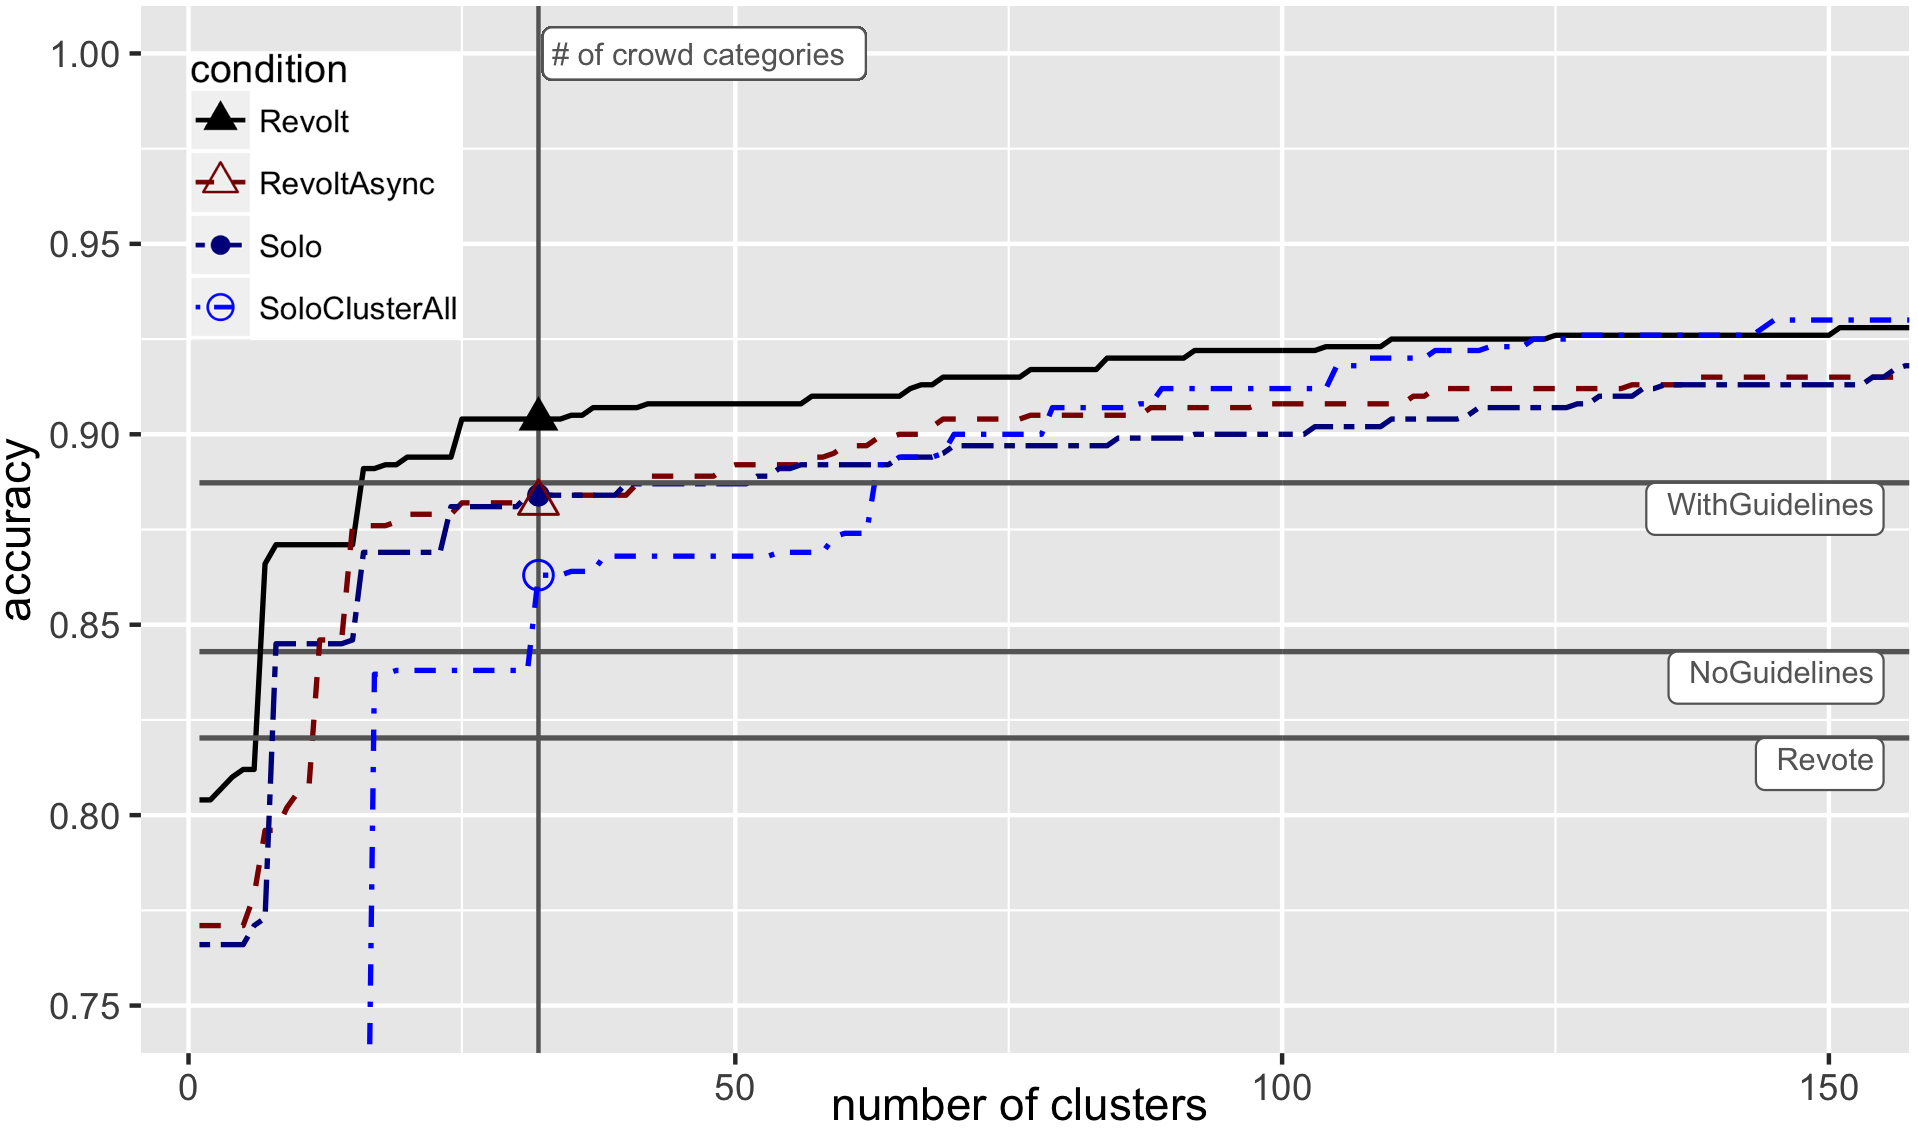
\includegraphics[width=0.7\columnwidth]{Chapters/Revolt/figures/curveR2.png}
	\caption[Accuracy of different approaches as a function of post-hoc requester effort.]{
	Accuracy of different approaches as a function of post-hoc requester effort (i.e., number of clusters) for the Car1 dataset. 
	}
	\label{fig:curve}
\end{figure}


In addition to presenting crowd-generated categories, Revolt (and its variant conditions) can also algorithmically produce clusters of uncertain items at various levels of granularity for requesters to review (see the Revolt Section). As a result, requesters can vary the amount of effort they are willing to provide to produce final label decision boundaries in these conditions. Therefore, for these conditions, we also report on accuracy achieved at various levels of post-hoc requester effort. As an example, Figure~\ref{fig:curve} shows how the accuracy of Revolt changes for different amounts of requester effort required to assign labels (estimated by number of clusters needing labels) on the \emph{Car1} dataset. For this example, receiving requester input for 32 categories produced by Revolt (see vertical line in Figure~\ref{fig:curve}) achieved an accuracy higher than the upper bound WithGuidelines baseline, while other conditions did not. 

We compare the accuracies of different conditions in two ways. In Table~\ref{tab:accuracy}, we compare conditions at a fixed amount of post-hoc requester effort (i.e., the number of clusters needing examination by the requester). We fix effort to be the number of categories generated by the crowd under the Revolt condition for each dataset. For example, for the \emph{Cars1} dataset, we compute accuracy at the point where 32 clusters would need to be examined. The accuracy results presented in the \emph{Cars1} row in Table~\ref{tab:accuracy} therefore corresponds to a vertical cut of Figure~\ref{fig:curve} at the 32 number of clusters mark. To compare different conditions and baselines, we fit one generalized linear model per baseline, predicting correctness as a function of condition, with dataset as an additional factor to account for item variation. Both models significantly improve fit over a simpler model with dataset
as the only variable (X2(5)=160.1, $p<0.01$, and X2(5)=180.9,
$p<0.01$). 
Using the models, we ran general linear hypothesis tests for pairwise comparisons between conditions, and used Tukey's honestly significant difference as the test statistic. 
The models showed both Revolt and RevoltAsync to be significantly more accurate than the lower bound NoGuidelines condition (B=0.56 and 0.38, both $p<0.01$) while no significant differences were found when comparing to the upper bound WithGuidelines condition (B=0.05 and -0.13, p=0.99 and 0.63).


In addition to using a fixed numbers of clusters, Figure~\ref{fig:accuracy} shows the of accuracy improvement rate of each condition under different levels of requester effort relative to the NoGuidelines baseline. Since the smaller datasets only had less than 30 uncertain items, for conditions that generate rich structures (Revolt, RevoltAsync, Solo, and SoloClusterAll) we show the accuracy improvement rate for 10, 15, 20, and 25 post-hoc judgments for the smaller webpage datasets, and 10, 20, 30 for the larger image datasets. We also report the accuracy improvement for the WithGuidelines and Revote conditions that do not require post-hoc judgments. 





%\saleema{Needs work. State the goal (need to measure cost), then the problem (couldn't compare because of different implementations, then solution (estimating one with the other)}

%Revolt produces reusable structures that generates accurate training labels without the efforts of guidelines creation. However, one critical question is the cost of such system comparing to traditional approach and the different conditions. 
In our experiments, \$3 were paid to each worker for participating in a batch of Revolt, Revote, Solo, SoloClusterAll conditions, where \$1 was paid as base payment for completing the first stage, and \$2 bonuses were added for completing the rest of the stages. For the RevoltAsync condition, \$1 was paid for each Vote and Explain task. We adjusted the number of items in each batch so that crowdworkers could finish batches under 20 minutes including time spent waiting for other crowdworkers. Each batch in the image datasets contained around 60 items while each batch in the webpage datasets contained around 27 items. For the baseline conditions, we paid \$0.05 for labeling one image, and \$0.15 for labeling one webpage. 

We also compared cost of each condition in terms of crowdworker work duration (Figure~\ref{fig:runtime}). For our Revolt, Revote, Solo and SoloClusterAll, we measure work duration directly by tracking crowdworker behaviors using our external HIT interface, tracking mouse movements to identify the exact time crowdworkers started working after accepting the HIT. Our NoGuidelines, WithGuidelines, and RevoltAsync conditions were implemented via the Mechanical Turk form builder feature. While Mechanical Turk does report work duration, crowdworkers often do not start work immediately after accepting a HIT. To correct for this, we approximate the work duration for these interfaces in the following way. We approximate the work time of the NoGuidelines and WithGuidelines conditions (our baseline conditions) using the timing statistics collected from the Vote Stage of the Revolt workflow, as the crowdwork involved in these baselines are of the same nature as the Vote stage. We similarly approximate the total work duration for the RevoltAsync condition by using the timestamps from the Solo condition (where crowdworkers provided explanations for each item), and multiplying the average duration with the number of uncertain items identified for each dataset in this condition.
 




%\ece{Do we want to discuss the reusability of the data anywhere? Do we collect data for two versions of the data set separately or collect the data once and then customize it for each data set using requester input? If it is the second one, it is a good argument for reusability of labels and we should emphasize that. }


%\saleema{Joseph, this section needs work. 1) You're mixing Results with Discussion. Typically Results are just where you present raw data and any stats you may have. Then in the Discussion you discuss your interpretations of the results. You can either try to separate the two or keep it, but then you have to figure out what to do with the current Discussion. 2) The subsections are not clear. First, avoid subsubsections where possible. If you want to keep Results mixed with Discussion, you shoudl just have a bunch of subsections such as: "Revolt vs Traditional Labeling", "Forcing Crowdworkers to Choose", "Benefits of Real-time Collaboration". For each of these you can mix the accuracy and cost results and discussion.  3) I'm worried about the Cost Analysis section. In particular, the formulas in Table 4 are cool in theory but without estimates for each T* I think you might be opening yourself up to reviewer criticism. Its not really that helpful wihtout the estimates anyways. It also makes the worktime per item analysis weird because its clear from the formulas that in most cases wortime is not uniform across N. You might want to consider removing this and just talk about the monetary cost (when will that be in??) and worktime per item in each of the subsections if you end up mixing accuracy and cost.}

\begin{figure}[ht]
	\centering
	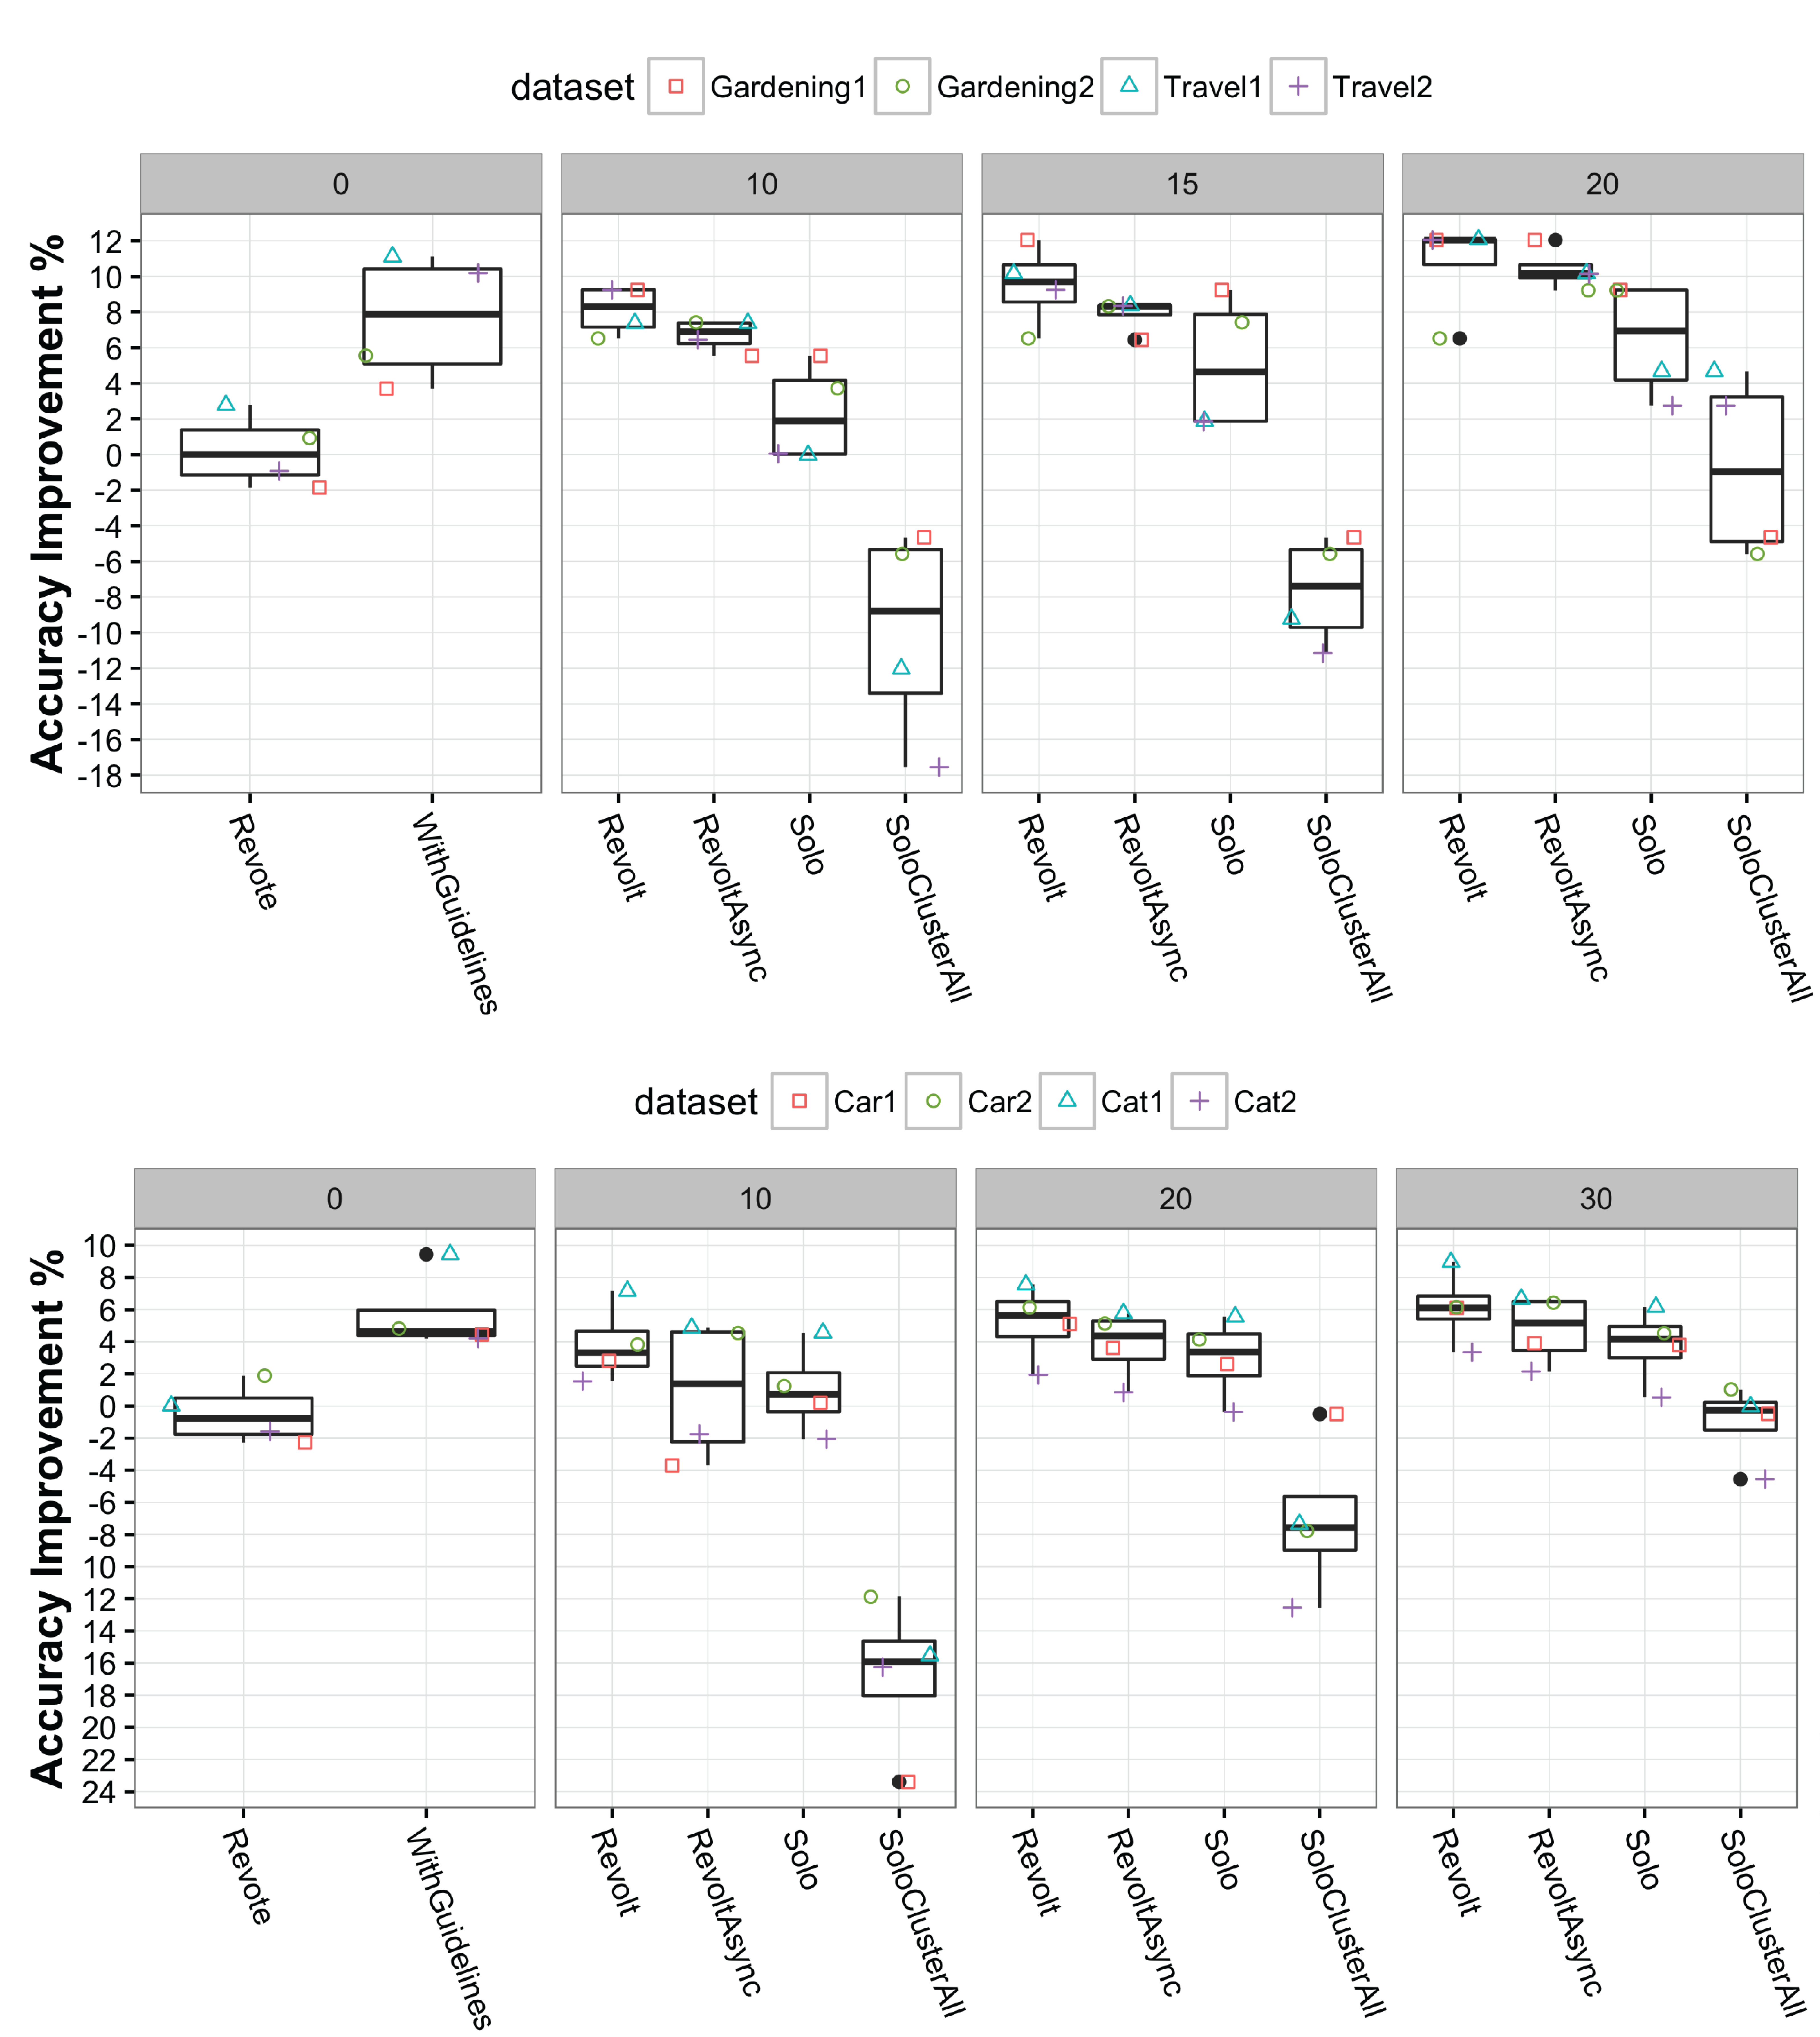
\includegraphics[width=0.7\columnwidth]{Chapters/Revolt/figures/haccuracy2.png}
	\caption[
	Accuracy improvement as a function of requester effort. 
	]{
	Accuracy improvement of different conditions over the NoGuidelines baseline as a function of requester effort. 
	}
	\label{fig:accuracy}
\end{figure}


%\subsection{Labeling Accuracy}

\subsubsection{Revolt vs Traditional Crowdsourced Labeling} 

%\saleema{NoGuidelines is not really a realistic scenario. I would go back to the conditions, explain that NoGuidelines should be considered a lower bound since in most traditional uses of crowdsourcing, some guidelines are provided. That way NoGuidelines is presented as a lower bound and WithGuidelines is an upper bound. Then revise this section accordingly  and say that the real traditional crowdsourcing falls somewhere in between. Nevertheless we can see that Revolt performs etc....}

In both traditional crowd-based labeling and Revolt, requesters examine uncertain items to refine the label boundaries. However, in Revolt, this is done at the category level in a post-processing step as opposed to reviewing items, refining instructions, and launching more tasks in a loop. The latter may lead to wasted work, particularly when refinements require workers to relabel the same items. In Revolt, structures captured from crowdworkers during labeling allow requestors to refine label boundaries post-hoc without having to launch more tasks.

When compared against the NoGuidelines condition (the lower bound of traditional crowdsourced labeling), Revolt was able to produce higher accuracy labels across all eight datasets (Table~\ref{tab:accuracy}). 
The generalized linear models also showed both Revolt and RevoltAsync to be significantly more accurate than the NoGuidelines condition.
The comparison of the NoGuidelines and WithGuidelines conditions shows that comprehensive guidelines indeed increase labeling accuracy across all eight datasets (Figure~\ref{fig:accuracy}), but at the cost of the effort needed to create comprehensive guidelines in advance. 
%This result supports the assumption that task uncertainty can also be an important factor for low quality results in crowdsourcing. \saleema{This last sentence comes out of nowhere and doesn't explain how it imapcts anything. Expand on this perhaps in its own section or at least in its own paragraph.}
In contrast, Revolt was able to produce comparable accuracy without any guidelines. In fact, in 6 out of the 8 datasets we tested, Revolt was able to produce labeling accuracies slightly higher than the upper bound baseline 
(Table~\ref{tab:accuracy}). The generalized linear models also showed that neither Revolt nor RevoltAsync were significantly different than the upper bound condition (B=0.05 and -0.13, p=0.99 and 0.63).
This suggests that Revolt can outperform current best practices for crowdsourcing training labels where guidelines provided by the requesters are likely to be less comprehensive than the ones provided in the WithGuidelines condition. That is, Revolt shows promise to improve the quality of labeled data collection while removing the burden of comprehensive guideline generation by making use of collaborative crowdsourcing approaches.


%\subsection{Reusing the Rich Structures}

%\saleema{Here you can also add a bit about reusability as Ece suggested. You can even present your results on using different guidelines for the same results to show reusabiliyt. Then you can explain that Traditional doesn't transfer to diffrent guidelines. You could even add a subsection about it called Reusability of Revolt Results.}


\begin{figure}[ht]
	\centering
	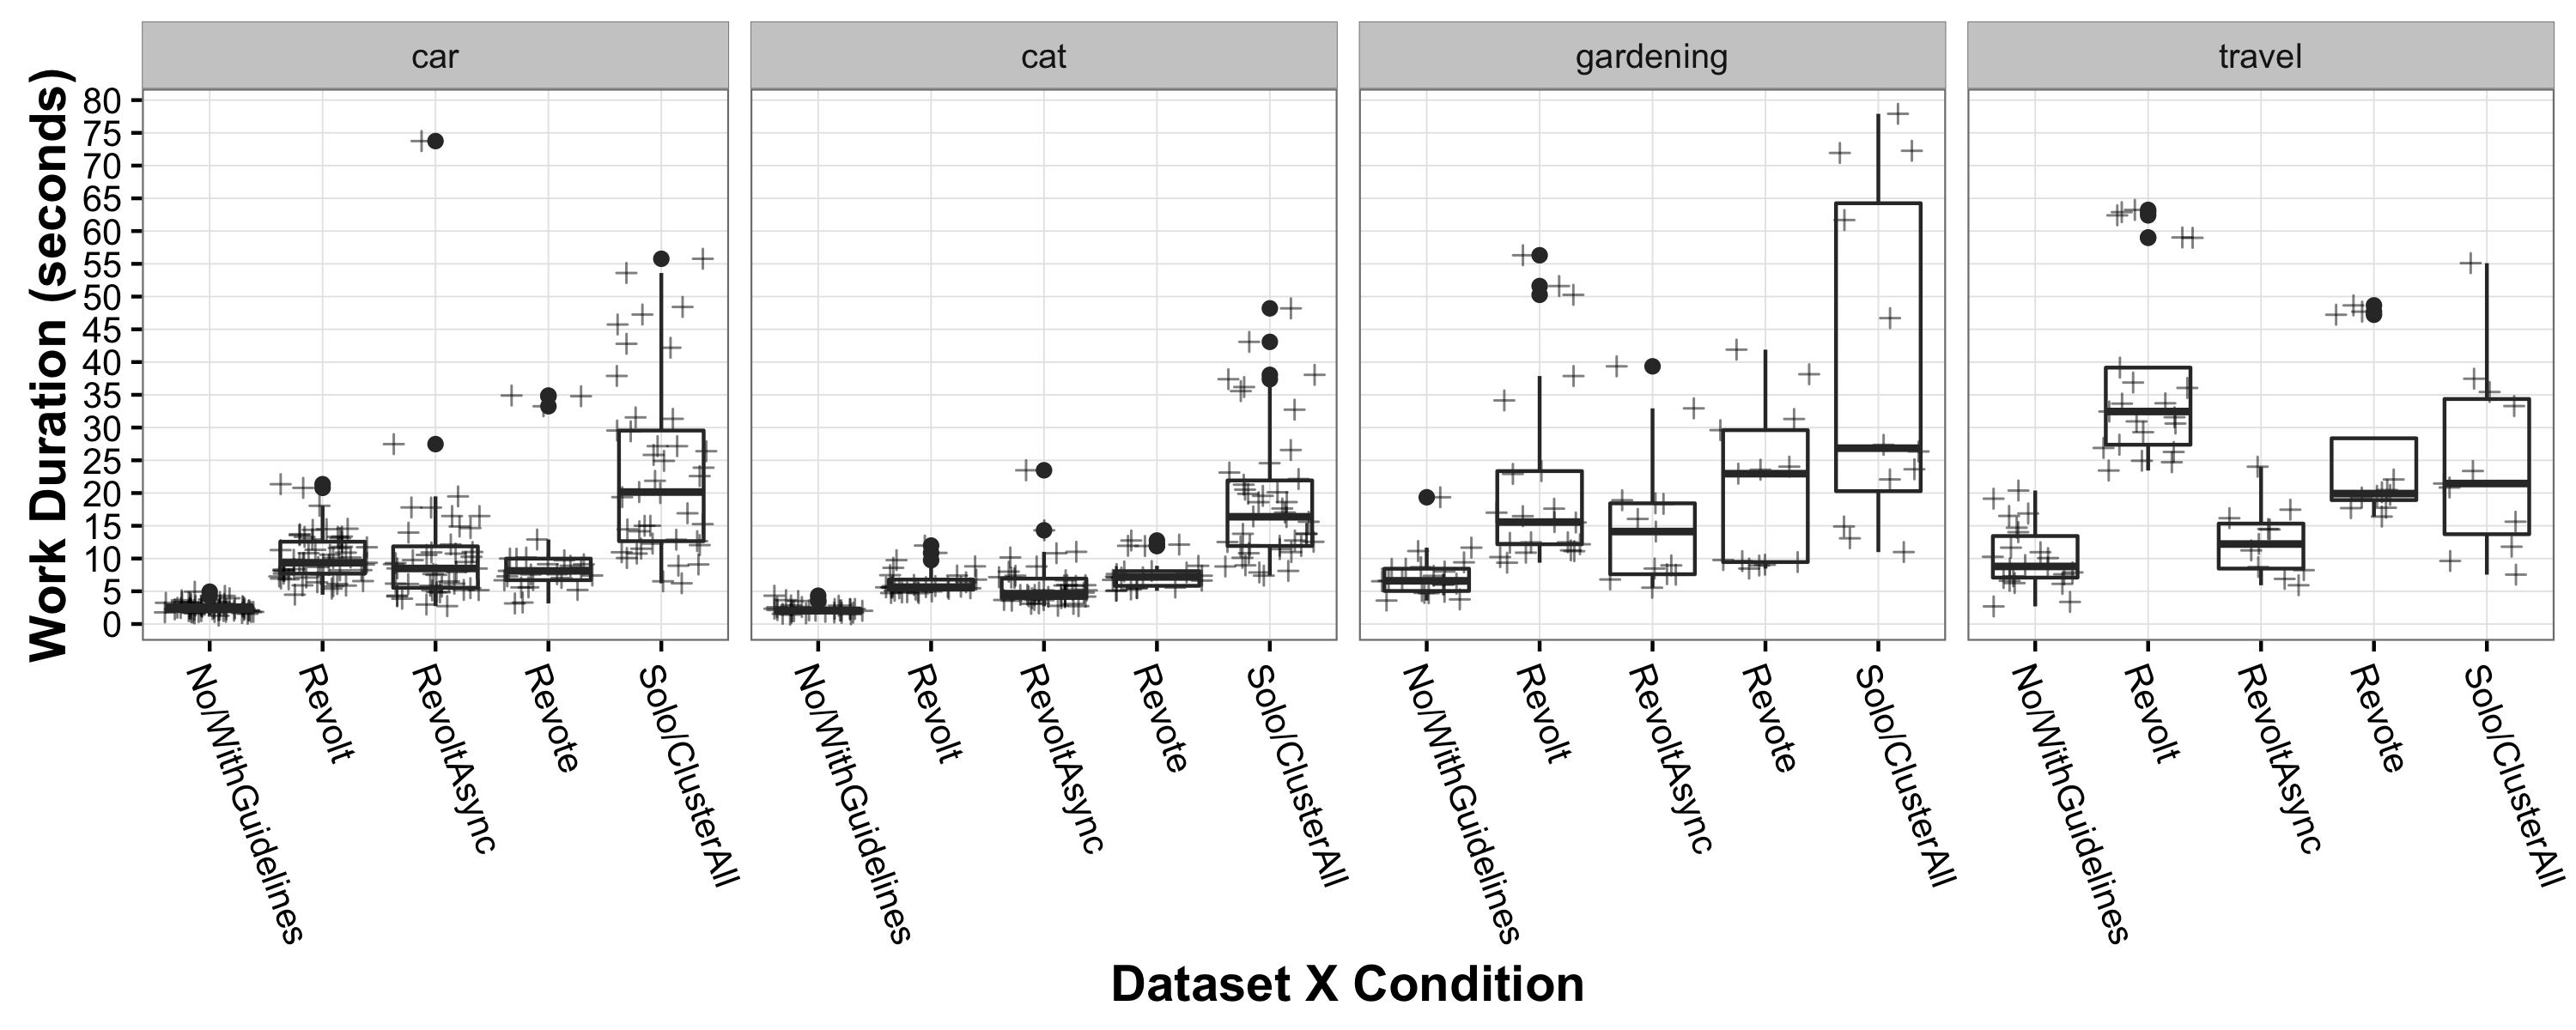
\includegraphics[width=1\columnwidth]{Chapters/Revolt/figures/runtime.png}
	\caption[
	Work duration of each crowdworker under different conditions. 
	]{
	Work duration of each crowdworker under different conditions, normalized by the number of item in each batch. 
	}
	\label{fig:runtime}
\end{figure}


\subsubsection{Forcing Crowdworkers to Revote} 

An alternative way of explaining why we see uncertain items with conflicting labels in Revolt's Vote Stage is that crowdworkers could converge on true concepts for all items but they are simply making mistakes while labeling. To test this, the Revote condition allowed crowdworkers to reconsider their labels after seeing explanations from others, providing the opportunity to correct mistakes.
While previous work has shown accuracy improvement using this strategy under a scenario where clear guidelines were given to pre-trained crowdworkers \cite{drapeau2016microtalk},  
%\saleema{I'd reverse the following two sentences. State your result and then state that this is a contradition to previous work and then explain what your hypothesis is about it}
results from our study showed that the Revote condition did not improve labeling accuracy compared to the NoGuidelines lower bound baseline (B=0.03, p>0.99), with near zero median accuracy improvement (Figure~\ref{fig:accuracy}).  This suggest that in scenarios where it is infeasible to generate comprehensive guidelines to guide workers towards a single correct answer, accuracy cannot simply be improved by quality control on individual workers; instead allowing crowdworkers to inform the requesters about their confusions and discoveries may be a better strategy than forcing them to make arbitrary decisions and then performing post-hoc quality control.
%\saleema{So in the previous work where accuracy was improved, did they assume a single correct label? If so, then are you disproving their result? Or did they do something slightly different. You have to be careful aobut the distinctions you make here.}

\subsubsection{Benefits of Collaborative Crowdsourcing}

Traditionally, crowdsourcing techniques require independent crowdworker judgments and do not permit knowledge sharing. 
In this work, we investigated the benefits of collaborative crowdsourcing by allowing limited and structured communications between crowdworkers. Our collaborative conditions (Revolt, RevoltAsync, Revote) presented crowdworkers with different combinations of conflicting judgements, justifications for the conflicting judgements, and proposed structures (i.e., category names) from other crowdworkers, either synchronously or asynchronously. On the other hand, in NoGuidelines, WithGuidelines, Solo, and SoloClusterAll conditions, workers were not presented with any judgments from others.

%\ece{Isn't it the case the Revolt sync does better in many conditions? Then we should say that instead of saying comparable. Because if accuracies are comparable, it makes no sense to use Revolt instead of Revolt async. It is important to highlight the trade-off between accuracy and time if it exists.  }
%\saleema{The improvements are very small and without stats to show that its better its a stretch to argue for Revolt over RevoltAsync. I'd be okay with us saying "slightly better" or something.}
Comparing Revolt to RevoltAsync, Revolt with synchronous stages performed slightly better than RevoltAsync at the cost of slightly higher worktime (Figure~\ref{fig:runtime}), but the difference was not significant (B=0.18, p=0.28). Comparing collaborative and non-collaborative conditions, results show that both Revolt and RevoltAsync outperformed the non-collaborative Solo condition for each  dataset we tested (Figure~\ref{fig:accuracy}). Based on the generalized linear models, the real-time collaborative Revolt condition achieved significantly higher accuracies than the  
non-collaborative Solo condition, while the RevoltAsync variant did not (B=0.24 and 0.06, p=0.04 and 0.97). 

Interestingly, we initially expected the RevoltAsync condition would yield poorer results compared to the non-collaborative Solo condition due to cognitive dissonance (i.e., asking one crowdworker to explain the label of another). However, the results showed no significant difference between the two conditions. On the other hand, the non-collaborative SoloClusterAll condition, where explanations were collected for all items to cluster both certain and uncertain items, performed worse than the lower bound baseline. These results suggest that identifying and presenting disagreements is an important factor for eliciting meaningful explanations, even when the disagreements were presented to different crowdworkers in an asynchronous setting (Figure~\ref{fig:accuracy}). 

%To investigate the benefits of real-time collaborative crowdsourcing, we also compared Revolt to variants that removed the real-time and collaborative components (RevoltAsync, Solo, SoloClusterAll). Results suggest Revolt outperformed its non-collaborative variants when having the same amount of post-hoc requester effort (Figure~\ref{fig:accuracy}), suggesting real-time collaboration might be a key factor contributing Revolt's accuracy improvement. Comparing the three non-collaborative conditions, the SoloClusterAll condition that clustered both certain and uncertain items performed the worst. This suggest identifying certain and uncertain regions of the data is an important component of Revolt, and clustering all items in attempts to correct the unanimously voted errors may not be an effective strategy. \saleema{This is not an explanation. This is just a result. Give a hypotheses as to why you think clustering all the data didn't work. Perhaps look at your clustering results to give examples of where this might break down.}



%\begin{figure*}[!ht]
%	\centering
%	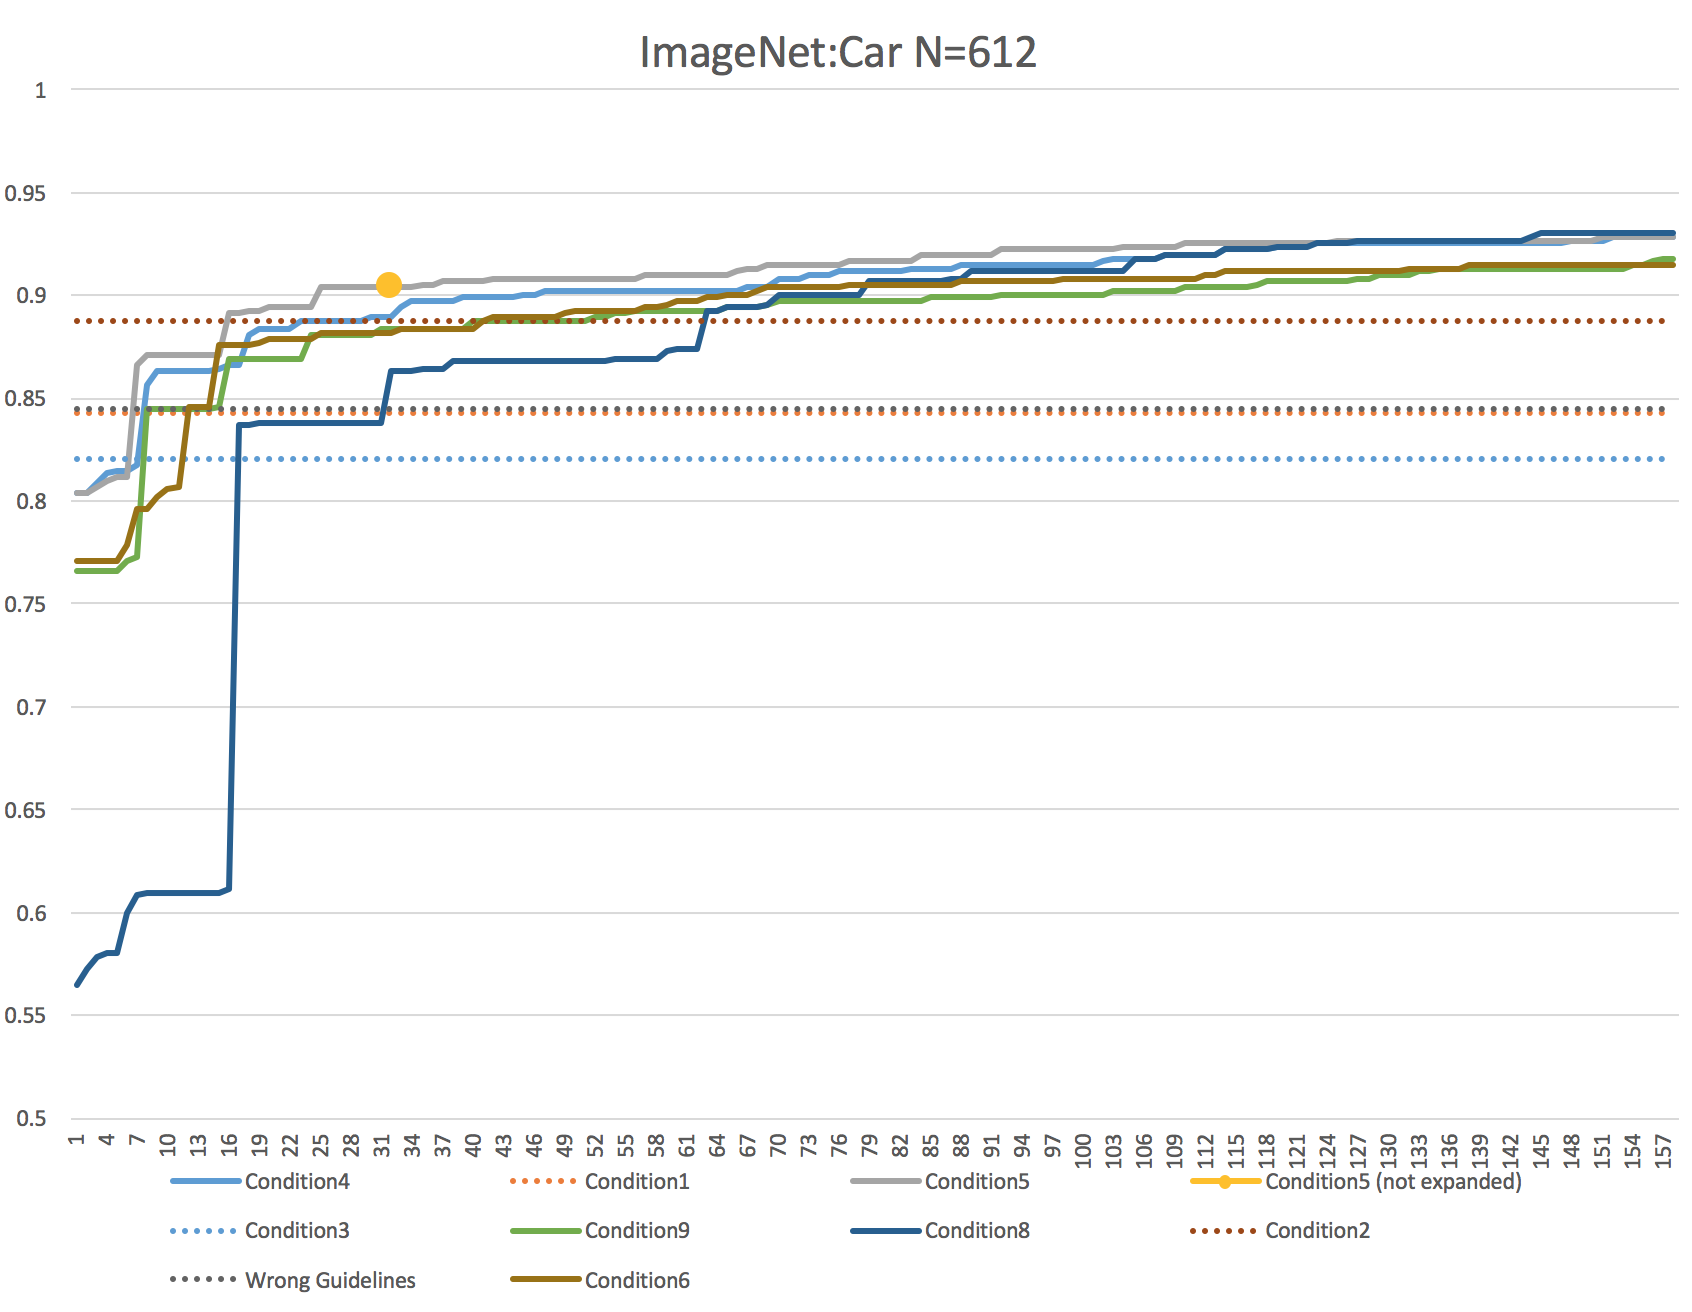
\includegraphics[width=1.0\columnwidth]{figures/dataset1.png}
%	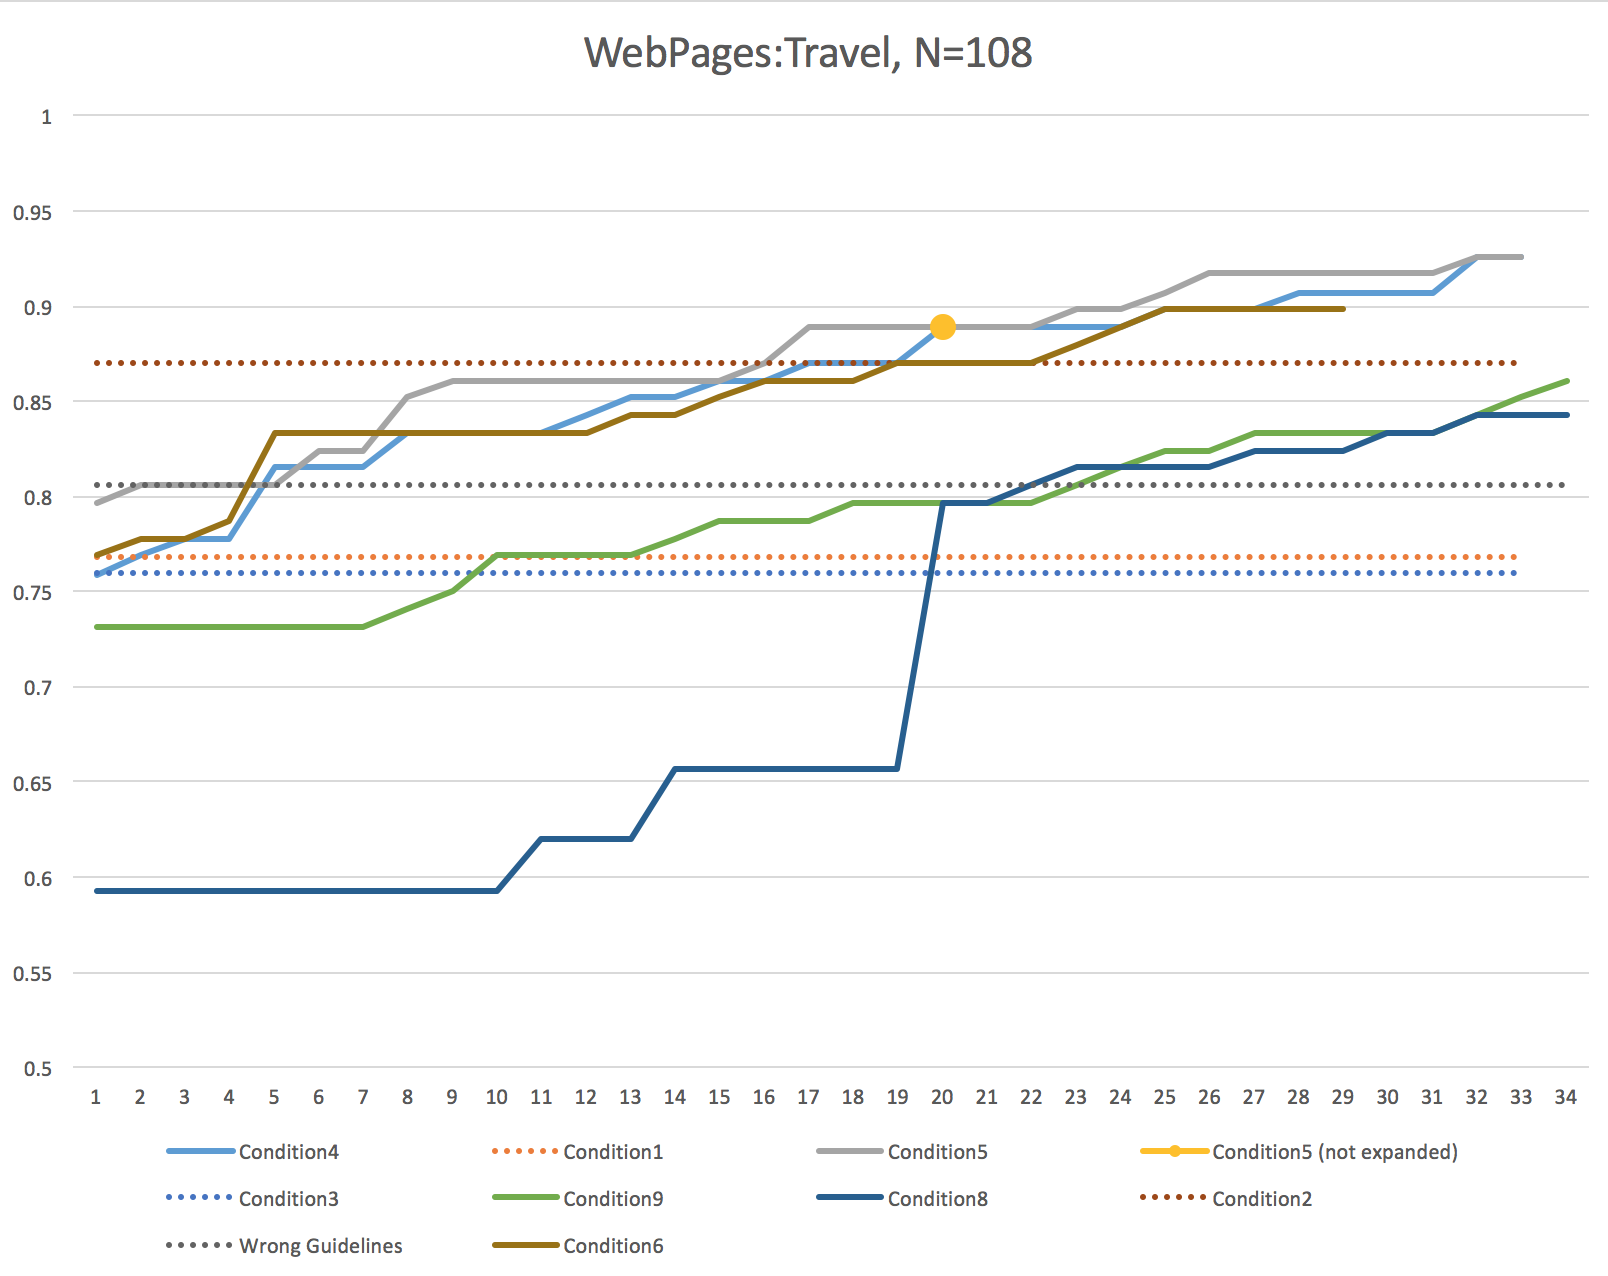
\includegraphics[width=1.0\columnwidth]{figures/dataset2.png}
%	\caption{
%	}
%	\label{fig:accuracy_curve}
%\end{figure*}




\subsubsection{Cost Analysis}


In general, items in the webpage datasets took longer to label compared to items in the image datasets. This is to be expected since webpages typically contain both text and images and therefore often require more effort to comprehend (Figure~\ref{fig:runtime}). 
Comparing different conditions, traditional labeling (WithGuidelines, NoGuidelines) that only required crowdworkers to label each item had the lowest work times, and the real-time collaborative conditions, Revote and Revolt, had similar and higher work times. This suggests categorizing or re-labeling items has similar costs, but creating rich structures for post-hoc requester judgments can lead to better accuracies. The RevoltAsync condition showed lower work time compared to the Revolt condition. This is also to be expected since crowdworkers did not need to wait for others during the task for progress synchronization. The non-collaborative workflow conditions Solo and SoloClusterAll has the highest work time since it required explanation of all certain and uncertain items. Therefore, using the voting stage to identify uncertain items and guide efforts on structure generation can improve accuracy while also lowering cost.

One concern for synchronous collaborative crowdsourcing is crowdworkers idling or returning the HIT before the task is competed. This was especially important since we did not include a method for using labels from groups with missing labels. In sessions with drop-outs, we paid the crowdworkers and discarded their labels. In fact, the first prototype of Revolt had a high dropout rate of around 50\% (i.e., half of the crowdworkers did not complete the three stages), making it infeasible for practical use. Through an iterative task design process, we observed the following mechanisms being effective for reducing drop-outs: Explaining the collaborative nature of the task, providing time estimates in the task instructions, adding example items in the preview screen so crowdworkers knew what to expect if they accepted the HIT, sending desktop and audio notifications to help coordinate workers, and giving clear progress indicators throughout the tasks (e.g., current bonus amount, number of remaining stages, and the amount of bonus for completing each stage). In the final version of the task with these mechanisms, the dropout rate was lowered to an average of around 5\% for the eight datasets presented in this chapter.

\section{Discussion}

%We compared our conditions using datasets of variety formats (images, webpages) and size (around 100 and 600 items). We used \emph{cars}, \emph{cats}, \emph{travel}, and \emph{gardening} to show that uncertainty can exist in crowdsourcing labeling tasks even for seemingly simple and generally familiar concepts (Table~\ref{tab:accuracy}). \saleema{In the discussion, reiterate this point and say that we show differences even for seemingly simple concpets. we would expect the differences to become even more pronounce for mor complicated concepts}

%\saleema{Much of this paragraph will be redundent if you merge the discussions from the previous section with this.}We tested Revolt against 6 baselines and variant conditions using 8 gold-standard datasets with up to 600 items consisting two different formats (webpages and images).
%Experimental results suggest that Revolt can to produce high quality labels without the need for the requesters to engage in the difficult task of guidelines creation. The real-time and collaborative nature is also beneficial as evidenced by comparing Revolt to its asynchronized variants.

%\joseph{note: testing different redundancy} 

%\joseph{note: matching worker with the same skill level to avoid waiting time.} 

%\saleema{I think these first two paragraphs are eithr not relevant or out of place given the reframing. Can you add any comments about general limitations of Revolt plus Revolt Async? Or if you think Revolt still could have benefits for some reason, argue for why. Otherwise, just change this section title to Future Work}

%\saleema{This is too specific to one stage of Revolt and given that it might not be necessary, since RevoltAsync doesn't have it, why do we care? If you want to talk about this, relate it back to why you think Revolt is better than RevoltAsync}One obvious limitation is the strong ordering effect of Revolt's real-time categorization mechanisms. For example, if the category \emph{big cats} was created early in the process, Revolt might lose its hyponymous concepts such as \emph{lions} or \emph{leopards}, and the requesters would need to rely on the automatic clustering process to recover these concepts based on the explanations. Revolt also made the assumption that crowdworkers will be able to select the best category, which can potentially be challenging as the list of categories grow in length. Even when the assumption holds true, better categories could be added even after a crowdworker completed the task. Adapting previous crowd clustering approaches to  real-time settings or developing more sophisticated real-time crowd clustering methods are fruitful areas of future work.

 
%\saleema{This doesn't seem relevant anymore since the RevoltAsync condition doesn't require wiating and should be able to handle different reading speeds. I'd cut}Another limitation is when the items are difficult to comprehend by the crowdworkers. We encountered this limitation when trying to run Revolt on a dataset of legal and financial news, where crowdworkers were tasked to determine if the main theme of an article is about ``\emph{an legal issue for an organization}''. We found that the crowdworkers were reading items in this dataset at very different speed in each stage, making it difficult to estimate the right number of items per batch to avoid long waiting time. Ultimately, the inherent difficulty the dataset lead to high dropout rate, and Revolt was unable to finish labeling all items.

%\saleema{This is confusing. Your basically saying thta Revolt can't handle overly complex topics. Itsn't that the whole idea? What is a manageable set of catgories? How many wree produced here and is that more than the other cateogires? I would cut this unless you want to do a deep analyais. I think the problem is just the first part which is the different labeling speeds which increases wait time and therefore drop out rates. This is not something encountered in non-realtime systems. Give some ideas to counter this in future work such as perhaps estimating reading speeds of crowdworkers to match up skill level/reading speed levels to avoid dropouts. }
 


%\saleema{Restate main findings and takeaways. Revolt produces high quality labels without the need for guidelines. The real-time nature is helping as evidenced by our async results. Areas for improvement in the system E.g., stemming of category tags for better grouping, cleaning up labels post-hoc (some workers said they made mistakes in labeling). }

%\saleema{In the discussion section, be sure to talk about the limitations of our current technique (e.g., that the categorization is highly impacted by the order in which items and categories appear) and some of the other options we discussed about trying to improve this more (e.g., to get people to categorize at the right level). Use examples of poor categories from your results to seed this discussion. }

%\saleema{Discuss anything about the impact of dataset size or difficulty. You could mention the legal dataset here}

In this work we focused on designing Revolt's collaborative crowdsourcing workflow and evaluating whether the generated structures contain information with enough richness for label requesters to define accurate label decision boundaries. 
While we believe the proposed mechanisms of identifying uncertainty with disagreements and creating structures with explanations can generalize to multi-class scenarios, the added complexity to both the crowdworkers and the interfaces should be studied further. Research is also needed to design a requester-facing interface depicting these structures and to compare requester effort in post-hoc analysis with guideline creation. 

%\ece{what was the pain point you were trying to address if they already had guidelines? Are you testing how good their guidelines were?}
To gain insights into these future directions, we conducted a small follow up experiment where we ran Revolt on data needed by a group of practitioners from a large technology company for a real machine learning research problem. 
This group required 300 items from the publicly available 20 Newsgroup Dataset \cite{Newsgroups20} to be labeled as being about ``Autos'' or ``Not Autos''.
Prior to our study, the group of three practitioners already spent approximately 2-3 hours each to browse through some of the data and then about 1-2 hours to generate and iterate over the guidelines. This is a typical process for guidelines creation analogous to previous work  \cite{wiebe1999development}, and should represent a realistic scenario somewhere between our lower bound NoGuidelines and upper bound WithGuidelines conditions. Because the practitioners already had some idea of how they wanted the dataset labeled, we ran Revolt with their guidelines. %\saleema{Joseph I reverted this. We don't want to say that this is a more realistic scenario. You cut out the bit later on about how the guidelines were actually harmful. But I think the fact that we still surfaced a bunch of new categories given the guidelines shows that this can be useful even with guidelines. You could add a line about that if you think its necessary.} 
%(e.g., "buying, owning, driving, maintaining and/or understanding cars is about autos", "mentioning autos as setting, background material, or comparison in a discussion that is clearly focused on another topic should not be considered as about autos").
%Because the group already had some ideas about how they wanted the data to be labeled as a result of the guideline creation process, we ran Revolt with their guidelines in the instructions. 

We presented Revolt's results to one member of the research group and asked them to examine the resulting structures. Interestingly, 93 out of the 300 items (31\%) were inconsistent even though we gave crowdworkers guidelines about how to label, underscoring the difficulty of creating comprehensive guidelines covering the subtleties in a dataset. These items surfaced 23 unique categories and, to the practitioner's surprise, 70\% were not covered in the original guidelines (e.g., auto accessories, insurance, intoxication). 7 of the categories were mentioned in the guidelines with explicit instructions about how to label (e.g., driving, buying/selling, auto repair), indicating either failure of some workers to learn the guidelines or failure of the guidelines to capture the complexity of these categories. 
For example, one of the items categorized as driving was about which side of the road people should drive on. While this could be considered about auto driving, it could also be about driving other types of vehicles. %Worker explanations about this item surfaced this ambiguity: \textit{"While it was related to driving it wasn't related to Auto in itself. For instance, motorcycles could also be considered in this conversation."}, \textit{"This is talking about what side of the road people drive on and relating to car exports."}, and \textit{"I didn't think this one was pertaining to autos specifically, just roads in different countries."}
%For example, one of the items categorized as driving was about which side of the road people should drive on. While this could be considered about auto driving, it could also be about driving other types of vehicles. Worker explanations about this item surfaced this ambiguity: \textit{"While it was related to driving it wasn't related to Auto in itself. For instance, motorcycles could also be considered in this conversation."}, \textit{"This is talking about what side of the road people drive on and relating to car exports."}, and \textit{"I didn't think this one was pertaining to autos specifically, just roads in different countries."}
Reading crowdworker explanations helped the practitioner to better understand this ambiguity, and led them to second guess their original guideline about labeling driving related items as autos.  The practitioner we interviewed also suggested additional ways they wanted to use Revolt's results, such as removing ambiguous items or certain categories before training a model, or creating features around categories that surfaced. Further research is necessary to examine the potential for Revolt's rich structures to support these tasks.
%Importantly, while the practitioner would be able to reassign items Revolt flagged as driving to the "not auto" category, Revolt may have still assigned some driving related items to the "auto" category because they were in the guidelines. That is, reassignment in this case could lead to inconsistent labels and poor machine learning. One possible alternative technique for incorporating guidelines into Revolt when they are available could be to seed the list of categories visible to crowdworkers during Revolt's categorization phase to help them tag items according to the requester's desired instructions.

The practitioner also made several suggestions with respect to how one might design the presentation of Revolt's structures. First, an indicator of category quality or confidence based on the distribution of labels assigned by individual workers would have helped the practitioner prioritize which categories to look at first and how much to examine each category before making a decision (e.g., by reading individual explanations or viewing a few of the individual items within a category). Other suggestions included blacklisting certain items from the category list (e.g., ``autos'' surfaced as a category), presenting structures within hierarchical categories, and searching explanations for to find related items under different categories. Future research should consider these insights in determining how to efficiently present Revolt's structures to label requesters.


%\section{Conclusions}

%In this paper, we explored an alternative process of crowdsourcing training labels for machine learning by forming small, ad-hoc teams on crowdsourcing markets and allowing crowdworkers to engage in collaborative exploration of the uncertainty in datasets by exchanging prospectives using a synchronized three stage workflow. 

In this chapter, we presented Revolt, a new approach for generating labeled datasets for machine learning via collaborative crowdsourcing. Our experimental results comparing Revolt to traditional crowd labeling techniques demonstrates Revolt can shift the efforts of label requesters from a priori label guideline creation to post-hoc analysis of crowd-generated conceptual structures. This has several benefits including potentially surfacing new or ambiguous concepts unanticipated by label requesters, reducing the amount of crowdworker training and effort required to learn label guidelines, and allowing label requesters to change their minds about label decision boundaries without having to re-collect new data. 

%\section{Acknowledgments}

%The authors would like to thank Andrew Mao and Walter S. Lasecki for the insightful discussions, and Joel Chan for the assistance in analyzing the evaluation results.

%%% Local Variables:
%%% mode: latex
%%% TeX-master: t
%%% End:


%\Chapter{SearchScape}{An Entity-centric Interactive Search Landscapes}
%\label{chap:searchscape}
%
While \cref{chap:alloy} explore ways to identify topical-based options for scenarios that involves deep understanding of a handful of different solutions, such as gardening, pluming, and physics, this chapter explore a different set of exploratory search scenarios where there are a much larger number of entity-based options available. For example, planning a trip or shopping for products where it can involve intense cross referencing of multiple sources for a large set of entity options. One has to determine the popularity and trustworthiness of competing options and avoid missing valuable but less common options. Traditional search systems leave this task to users, while automatic result clustering approaches often fail to produce structures coherent enough to meet these needs. We introduce a novel approach that builds coherent topical landscapes from search results. By combining the rich but sparse representations of knowledge bases with word vector models that are shallow but dense in coverage, we produce structures more coherent than alternative approaches. We instantiate this in a prototype interactive system and explore which elements users find useful. Across three information seeking scenarios, we found that participants valued both the structure and distribution information provided by our system for complex exploratory searches and, surprisingly, simple searches as well.  
%    Whether planning a trip or researching medical symptoms, many complex exploratory search tasks involve scenarios where users are unfamiliar with the domain of interest, unsure about what the possible options are, and have difficulty knowing how popular or trustworthy those options may be.  Current approaches to supporting search either fail to address these needs or are limited by a dependence on the existence of well-structured metadata. We introduce a novel approach to extracting structure from arbitrary web content (e.g., in a set of search result pages) and explore the value such content can provide in helping users understand the information landscape. The intuition behind the approach is that knowledge graphs and ontologies provide rich but sparse representations that can be used to structure search landscapes, while word vector models are shallow but work on a wide variety of terms and entities. We combine these methods to build interactive search landscapes that automatically discover relevant topics for a given query based on the content of the web pages and external knowledge sources, measure the distribution of topics across sources, and group topics into useful schemas. Across three information seeking scenarios we found that participants found our approach useful and an improvement to traditional search interfaces for complex exploratory searches and, surprisingly, simple searches as well.



%From simple fact-finding tasks to complex learning and information exploration tasks, people often rely foraging information online to make sense of the world today. Particularly, exploratory searches that involves learning in an unfamiliar domain can often be stressful and time consuming. While modern search engines do a great job at retrieving intended webpages in split seconds, searchers in these scenarios often do not have clear ideas about the exact information needed \cite{mar2006exp}.
%In contrast to previous work that focused on shepherding users to intended documents using structures in labeled corpora, we focused on 
%combining hand-crafted knowledge bases with machine learned semantic models to extract interpretable structures with good coverage
%from unstructured web content.
%This allowed us to surface the distribution of key subtopics, providing an overview of the information landscape. We embody this idea in an interface we called SearchScape, which allows searchers to gain quick overviews using the distribution of key subtopics, and interact with search results to dive into different subtopics. In an experiment with 210 participants and a 3x2 between subjects design, we tested SearchScape in a wide range of scenarios, and the effects of showing distribution information.
%Results showed that participants found SearchScape to be useful and an improvement to traditional search results interfaces, and that showing distribution of key subtopics was perceived as significantly more useful.



\begin{figure}
    \centering
    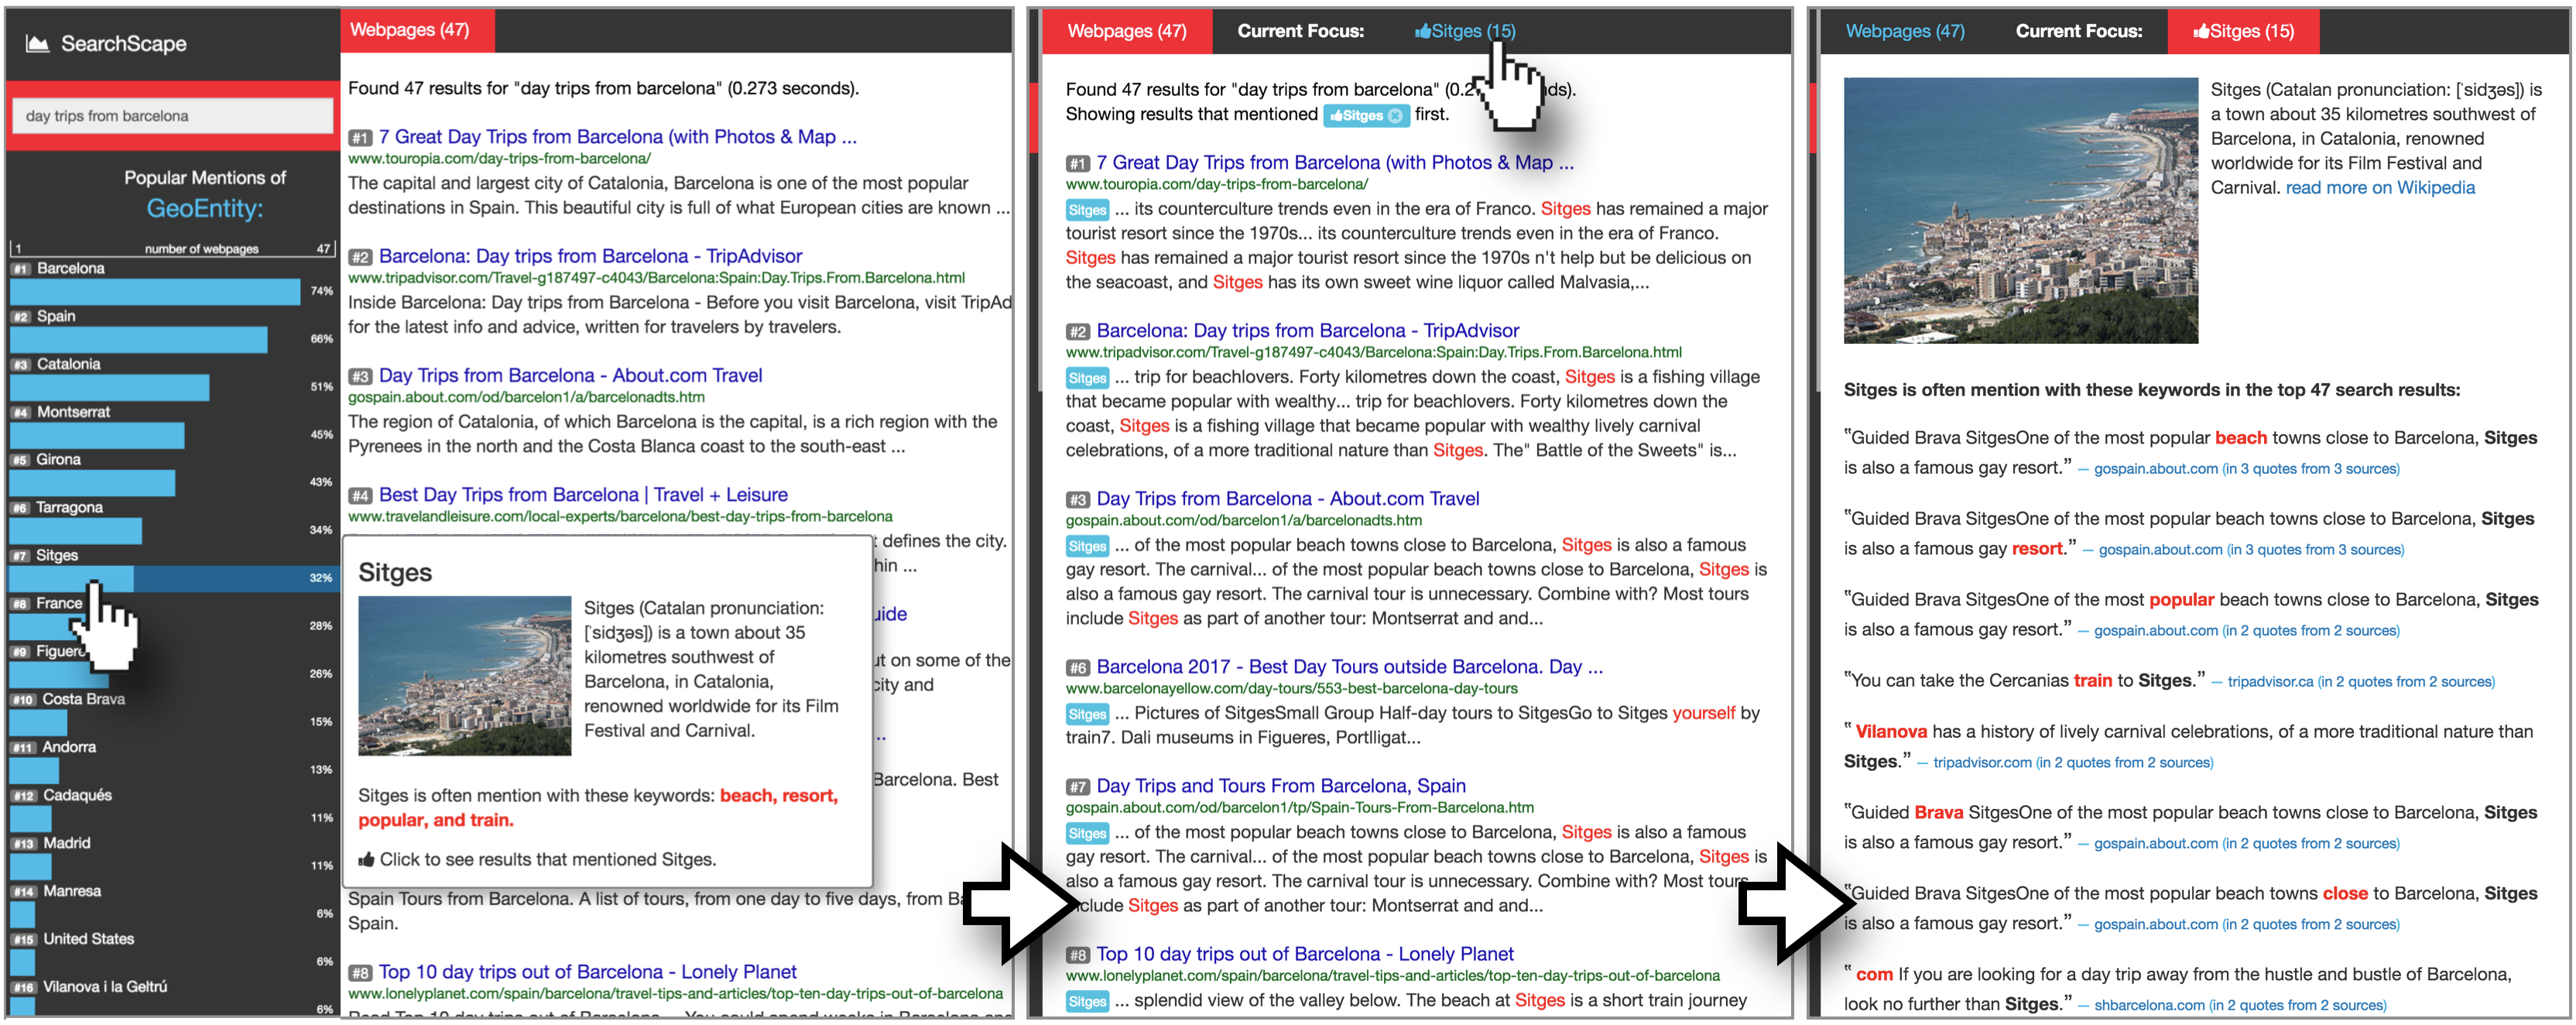
\includegraphics[width=1.0\textwidth]{Chapters/SearchScape/figures/main_old.png}
    \caption[An overview of the SearchScape system.]{An overview of the SearchScape system. The Document Panel on the right shows a ranked list of search results, while the Structure Panel on the left shows the distribution of automatically identified key concepts in the search results. Exploratory searchers can click on an item to filter the search results and see how the item of interest is mentioned across sources. Alternatively, they can also grouped these mentions using keywords were frequently mentioned together with the item of interest.}
    \label{fig:flow}
\end{figure}

\section{Introduction}

Consider an example of an exploratory search such as looking for the best day trips from Barcelona. Searching for this online returns a set of web pages primarily composed of lists of day trip destinations. These range from the popular beach town of Sitges to the less well known market town of Vic. However, looking at any single page raises a number of potential issues. A reader might want to know the relative popularity of each option: while Sitges appears many different sources, Vic appears in only a few, despite being given approximately equal weight on a top search result.\footnote{LonelyPlanet - Top 10 day trips out of Barcelona,  https://www.lonelyplanet.com/spain/barcelona/travel-tips-and-articles/top-ten-day-trips-out-of-barcelona} Conversely, a page may be missing a popularly cited option such as Sitges and the reader would have no indication they might be missing out.  Providing an overview of the range of options could also expose interesting options in the long tail that could be relevant to certain readers, despite not appearing in the top few results (e.g., a Utopian textile mill's church designed by Gaudi, Col\`onia G\"uell).  

To understand the prevalence of this problem, we conducted a pilot survey with 103 participants from Amazon Mechanical Turk (age between 20 and 63, M=36, SD=12, 60\% male and 40\% female, mostly from the US), focusing on their experiences when conducting complex exploratory searches. Around half of the participants reported having conducted more than four exploratory search tasks in the past two weeks, in which 17\% reported having conducted more than ten tasks. Our results reaffirm that 
when conducting exploratory searches, people read from multiple information sources to make sure they do not miss something important (84\%), look for more information about a topic from other webpages in the same search result (84\%), verify previously seen but uncertain information using multiple sources (88\%),
and get a sense of what's popular or important in the search results (76\%).
At the same time, many also found conducting complex searches can be stressful (60\%), and that they often end up with more browser tabs than they can manage efficiently (67\%). These findings are consistent with previous findings that shows that up to 33\% of this time is related to complex exploratory search tasks \cite{mar2006exp,kellar2007field,rose2004understanding}.



%To address these challenges searchers actively engage activities such as cross-referencing information across different webpages, identifying and learning important subtopics, planning out subsequent queries (cite), and synthesizing information gathered from multiple sources (cite something from KA).


Despite their importance and ubiquity, the activities described above are poorly supported by modern approaches. Recent advances in search interfaces have optimized for providing information as quickly as possible, such as knowledge cards in which an answer is surface directly on a search results page or visual carousels of possible options that a user can quickly click through. These approaches excel at finding specific information, but notably fail to address the activities involved in complex search such as cross-referencing information across different webpages, identifying and learning important subtopics, planning out subsequent queries, and synthesizing information gathered from multiple sources.

Meanwhile, research on supporting complex information seeking has attempted to address some of these activities through faceted navigation \cite{hearst2006design} and semantic web interfaces \cite{wilson2006mspace}. While useful in an environment with well-structured data, it's prohibitive to expand these approaches to support the unstructured Web \cite{bruce1999workplace,teevan2008challenges}.
%The most obvious challenge here involves the difficulty for computational approaches to automatically detect important subtopics and information items from the general and unstructured search results }. 
One promising direction has been using unsupervised clustering algorithms to automatically extract structures from search results, which have been found useful for separating relevant sources from irrelevant sources (e.g., differentiating fruit related from technology related results when querying ``apple'') \cite{zeng2004learning}. However, these automatically generated structures are rarely coherent enough to provide an overview of the space of useful information. Consider the top five clusters that Clusty (now yippy.com) shows for ``Day trips from Barcelona'': Spain, Europe, Cruise, Photos, Reviews. Even within the Spain cluster the subclusters provide no structure or coherence: Blog, Tours from Barcelona, Flights, Guided, Cordoba, Cultural, etc.  The topics for ``Guacamole recipes'' similarly do not provide any concepts of the same class: Mexican (country), Chef (profession), Health (topic), Blog (format), and Free (cost). While these structures may be useful for navigating to sources in different dimensions (e.g., websites for guided tour services, for photo albums, or for blog posts), they provide little utilities for comparing between options under the same dimensions. For example, comparing the popularity and the types of activities you can do in different locations when searching for day trip destinations, or compare the reviews and popularity of different guided tour services. Fundamentally, automatic structures often provide no structure to define a space -- there is no base for comparison and no understanding of relationships between concepts in their structure. 
At a higher level, faceted search and clustering approaches make better filers for people to zero in on what they know they are searching for (e.g., Apple the tech company), whereas we are instead trying to provide an atlas for exploratory scenarios (e.g., how popular are the different destinations, and how different sources describe them): a representative description of the space to help searchers learn about their options in the information space and how key concepts are distributed among the search results.

%However, a more subtle issue is that even when metadata exists to support computational approaches, the way this information is exposed (e.g., through facets or clusters) is often oriented towards directing people to specific pages rather than providing them with an understanding of the distribution of information in the query space in a way that more directly supports the examples above. 

%A third possibility is that adding this extra information may complicate the search interface in a way that is undesirable for searchers, providing insufficient value for the added complexity.

In this chapter we explore a novel approach for extracting coherent structures from arbitrary unstructured web content (i.e., in a set of web search results), and also how to present such structures to the users to provide an overview of the information landscape. We instantiate this approach in a prototype system called SearchScape, an interactive search result exploration interface. SearchScape dynamically identifies useful structures by combining external knowledge bases (i.e., Wikipedia\cite{bollacker2008freebase} and NELL\cite{carlson2010toward}), and machine learned unsupervised semantic models (i.e., Word2Vec\cite{mikolov2013efficient} and GloVe\cite{pennington2014glove}). The intuition behind this approach is that on the one hand, knowledge bases provide high quality entities and ontological frameworks, but often lack good coverage over arbitrary search results. On the other hand, unsupervised models provide substantial coverage, but can often be overly generalized and difficult to understand due to its lack of structure and incoherence. SearchScape combines the two to identify high quality categories from  knowledge bases that are easy to understand (e.g., Geographic Locations, or Agricultural Products), while expanding the coverage of these categories using automatically learned semantic models. In our first study, we find that structures produced by SearchScape for 50 different exploratory search queries was found to be significantly more coherent than structures produced by a search result clustering system.

Extracting coherent structure enabled us to further expose the distribution of key items of the same classes in the search results, in hopes that it can allow exploratory searchers to better understand all the options in the information landscape. For example, exposing the popularity of different \emph{location} items when searching for day trip destinations, or how common different \emph{ingredient} items are when searching for recipes.  In our second study, the overall system was found to be useful for three diverse scenarios including both exploratory and fact finding search. Further examination using a control condition hiding distribution information found that in exploratory situations showing distribution was significantly more beneficial to searchers.





\section{Related Work}


Several exploratory search interfaces have been developed in order to help searchers orient themselves in the information space, review and explore the different subtopics, and keep track of their overall progress \cite{hearst2009search,marchionini2000agileviews,patterson2001predicting,tretter2013searchpanel,morris2008searchbar}. Two closely related studies include Topic-Relevance Map and Exploration Wall, which explored ways to provide overviews of search results of academic papers using document keywords and entities and easily choose keywords to build up subsequent queries \cite{peltonen2017topic,klouche2015designing}. SearchScape also makes use of key entity mentions in the document for overview and drill-down purposes, but we automatically extract key items from the unstructured web using combined hand-crafted knowledge bases and machine learned unsupervised semantic models.

%In SearchScape, we retain the look and feel of standard web search engine, but included an extra side panel to provide a quick overview of the information space, and also to enable deep interactions with the search results. 




\subsection{Diversity and Distribution of Information}

%Ensuring that the users are exposed to a diverse set of  information is crucial for discovery-oriented exploratory search tasks, but researchers have also found that queries formulated for the same exploratory search tasks often yielded highly overlapping sources up to 50\% to 60\% \cite{qvarfordt2013looking}. Consequently, a collection of research has focused on helping exploratory searchers reach more diverse results without drastically changing the existing search paradigms and interfaces. For example, providing real-time feedback during query formulation by suggestion different subtopics (cite auto complete for exploratory), or providing real-time visual previews of the proportion of overlapping sources during query formulation \cite{qvarfordt2013looking}. Researchers have also focused on the ranking and re-ranking to increase the diversity of search results. 

Initially motivated to reduce redundant information in top search results produced by traditional relevance-oriented ranking algorithms, Carbonell et. al first introduced the idea of ranking search results to increase the diversity of information in the top results for scenarios where a large amount of potential relevant document exists in the corpus \cite{carbonell1998use}. More recent research has also explored how diversifying search results can benefit exploratory searchers (e.g., \cite{jin2013interactive}). Our perspective differs from these pure diversity-oriented ranking approaches, which optimize for showing as many different topics to the user as possible. We instead argue that the distribution of different topics and key entities can actually be a useful signal for exploratory searchers to judge the importance of different subtopics, and prioritizing their subsequent exploration. In this case, showing a uniformly diversified list of search results could actually give people an incorrect sense of the information distribution. For example, showing as many restaurant choices as possible can at the same time obscure a sense of how frequently each restaurant is mentioned. A similar idea was pointed out by Dang et. al, who proposed instead to diversify search results while accounting for the proportionality of information in the search result \cite{dang2012diversity}. In SearchScape we take a more direct approach than re-ranking search results and  present the distribution of extracted entities on the interface so that exploratory searchers can easily compare and evaluate the different subtopics in the information space.

%Jin et. al proposed to diversify the top search results in the first page so that users can get an overview of the information space, and re-rank the rest of the results based on which webpages the users visits \cite{jin2013interactive}. 

%Researchers in the fields of cognitive psychology, human-computer interaction, and information retrieval have made great strides on both understanding the process of exploratory searches and building systems and interfaces to better support exploratory search scenarios (bunch of cites).  

%SearchScape differs from traditionally faceted search systems in two ways: 1) We automatically inferring categories and entities using external knowledge sources, instead of relying on labeled corpora. 2) Traditionally facets were primarily used for navigation and finding items that meet specific criteria. We instead use ``facets'' primarily to give users a sense of the information space, to expose information distribution, to show different contexts of use, and generally for exploration.



%However, these faceted exploratory search systems all exploited corpora that were manually labeled with carefully designed categories and facets, such as authors and publish dates of books, genres and lengths of movies, or brands and prices of merchandises. Much of the techniques cannot be easily utilized for the general web due to both the unreliability of online information sources, and the lack of readily available metadata for online documents beyond titles and domain names. Past efforts on using crowdsourced editors to categorize websites, such as the Open Directory Project\footnote{DMOZ, https://www.dmoz.org/}, had also failed to keep up with the ever scaling of the web, and most have been discontinued. In addition, online documents often describe multiple items on the same page (e.g., \emph{top 10 compact cameras}), which can make it difficult to uniquely categorize a document under a single category (e.g., a facet of camera brands). Secondly, many past systems used high quality corpora that were assumed to be trusted by their users. For example, the the price and brand information of products on commerce websites, or the author and publish date information on publisher websites, when conducting complex exploratory search for unfamiliar domains on the Internet, most searchers are actively evaluating the trustworthiness of information sources they have encountered using different types of features, such as domain names, visual designs, and writing styles(?) (cite web/trust papers), and often validate and evaluate the importance of a new piece of information by cross-referencing multiple sources (cite??? Maybe something in KA?). For example, choosing a travel destination that were frequently mentioned favorably online, or paying attention to the frequently discussed term ``recurrent neural-networks'' when researching ``artificial intelligent'' online. This lack of support in modern search interfaces for discovery-oriented exploratory search scenarios has left users the heavy burden of figuring out the important subtopics in the space of information using just a linear ranked list of relevant webpages \cite{bruce1999workplace}, leading them to rely on external tools such as printing, and word processors to deal with the issues of organizing, managing and re-finding previously found information \cite{aula2005information,white2006supporting,morris2008survey,capra2010tools,kittur2013costs}. 

\subsection{Faceted Search for Structured Corpus}

Faceted search is perhaps the most commonly used search interface, in which users can filter results by selecting or deselecting categories or ``facets'' (e.g., products on an online shopping site). Although originally designed to help searchers efficiently narrow down on relevant sources and exclude irrelevant sources from their search results (e.g., showing only digital cameras of specific price range and manufactured by a specific company on an online shopping site), researchers have also found faceted search interfaces to benefit exploratory scenarios, where searchers are less certain about their information needs \cite{hearst2002finding,yee2003faceted}. Facets can provide an  overview of the different topics in the information space in addition to supporting drill-down on those topics \cite{yee2003faceted,capra2008relation,kules2009exploratory} and have been widely explored for corpora where metadata are readily available, such as images \cite{yee2003faceted}, music \cite{wilson2006mspace}, social media \cite{o2010tweetmotif}, library catalogs \cite{marchionini2006towards,kules2009exploratory}, and scholarly articles \cite{hearst2009nlp,dork2012pivotpaths,klouche2015designing}. However, in cases where metadata is not readily available, computationally inferring fine-grained facets (e.g., day trip destinations) remains a challenge, inhibiting the faceted interface from being expanded to support exploratory search on the open Web \cite{bruce1999workplace,teevan2008challenges}. Instead of requiring documents to be annotated with metadata, SearchScape uses a novel technique for automatically producing structures by inferring topics from unstructured web content by combining readily available knowledge bases and ontologies. Furthermore, we also explore the benefits of visually depicting the distribution of content across structures in helping the user better understand the information space.


\subsection{Automatically Identifying Structure}

More generally, numerous challenges have been identified \cite{teevan2008challenges} in developing structured search systems to better support exploratory scenarios without pre-compiled metadata. Researchers have long explored ways to extract structure by clustering search results using machine learning \cite{zamir1999grouper,zeng2004learning,hearst1996reexamining}, lexical and HTML patterns \cite{kong2014extending}, crowdsourcing \cite{ka,alloy,cascade}, or interaction techniques \cite{hearst1996reexamining,hearst1996visualizing,hearst1996visualizing}. However, a number of papers \cite{hearst2006clustering,chuang2012interpretation,alloy} point to the fact that automatically techniques, such as unsupervised clustering, can often produce incoherent structures that are difficult to comprehend by users unfamiliar with the domain of interest. Further, providing a quick overview using coherent structures can be critical in supporting early stages of the exploratory search process. This helps users get a sense of the information space, and further investigate subtopics that are interesting or important to the them \cite{mar2006exp}. Conversely, techniques that utilize human judgments via crowdsourcing or user interaction can produce structures that are more coherent, but do so at the expense of either additional time and monetary cost or user effort\cite{alloy,ka}.

Perhaps most closely related to our work in intent, MetaSpider extracts noun phrases from webpages to use as features for clustering webpages in search results into visualized topic maps using the Kohonen SOM algorithm \cite{chen2001metaspider,kohonen1998self}.
Instead of trying to identify structures solely based on information presented in the search results, SearchScape utilizes rich and readily available knowledge bases and ontologies to automatically identify dynamic but coherent structures that best fit the search results.
%First, SearchScape identifies topics relevant to the current search results from large sets of predefined concepts in knowledge bases using their ontological frameworks, and then extracts entities of those topics from the search results to generate coherent and interpretable structures.
In addition, instead of producing document clusters, SearchScape presents distributions of entities over documents in the search results, as an overview of the information space (e.g., list of day trip destinations and how often they are mentioned in the search results.)

%For example, the Scatter/Gather system allowed users to navigate and explore large collections of documents using an interactive hierarchical clustering paradigm \cite{hearst1996reexamining}. The TileBars system allowed users to define topic models using sets of keywords, and provide real-time visual feedback for exploring the topic distributions over documents in search results \cite{hearst1996visualizing}. On the other hand,  







\section{System Design}
The SearchScape system augments standard web search results with a list of dynamically identified concepts useful for the current query. This gives exploratory searchers the ability to first gain a quick overview of the information space and explore different subtopics. The system consists of two main components. First, SearchScape analyzes the content of all webpages in the search results to identify the latent structures in the information space leveraging existing knowledge base structures (which typically have higher accuracy but lower coverage) and expands them with unsupervised word vector models (lower accuracy but higher coverage). Then, the search results along with the identified structures are presented to the user through an interactive search result interface which visually presents the distribution of structures. In the following subsections, we will describe in detail our data sources, the back-end components, and the front-end interface.

\subsection{Data Source}

In an ideal setting, the back-end components of SearchScape would be integrated as a part of a general web search engine, so that content fetching, indexing, and analysis can be performed before query time. However, since it would require enormous time and resources to download and index the entire web to build a full-scale web search engine, we used a readily available API from a commercial search engine as our data source.\footnote{Bing Web Search API, https://www.microsoft.com/cognitive-services/en-us/bing-web-search-api} In the front-end, SearchScape focused on augmenting traditional web search results with automatically identified, task-specific structures using an interactive interface to better support exploratory scenarios. Similar to search engine back-ends, we also pre-fetch and pre-index webpages for a fixed set of queries by first retrieving a list of top 50 relevant webpages from the API, then download and extract the main content of each webpage to remove menus and advertisements using an readily available API\footnote{Mercury Web Parser, https://mercury.postlight.com/} and build an inverted-index file for each webpages \cite{baeza1999modern}.
Finally, we perform further analysis to identify task-specific structures as described in the next subsection.\footnote{Many academia alternatives also exist for webpage content extraction such as \cite{kohlschutter2010boilerplate}.}

\subsection{Identifying Structures}

\begin{figure}
    \centering
    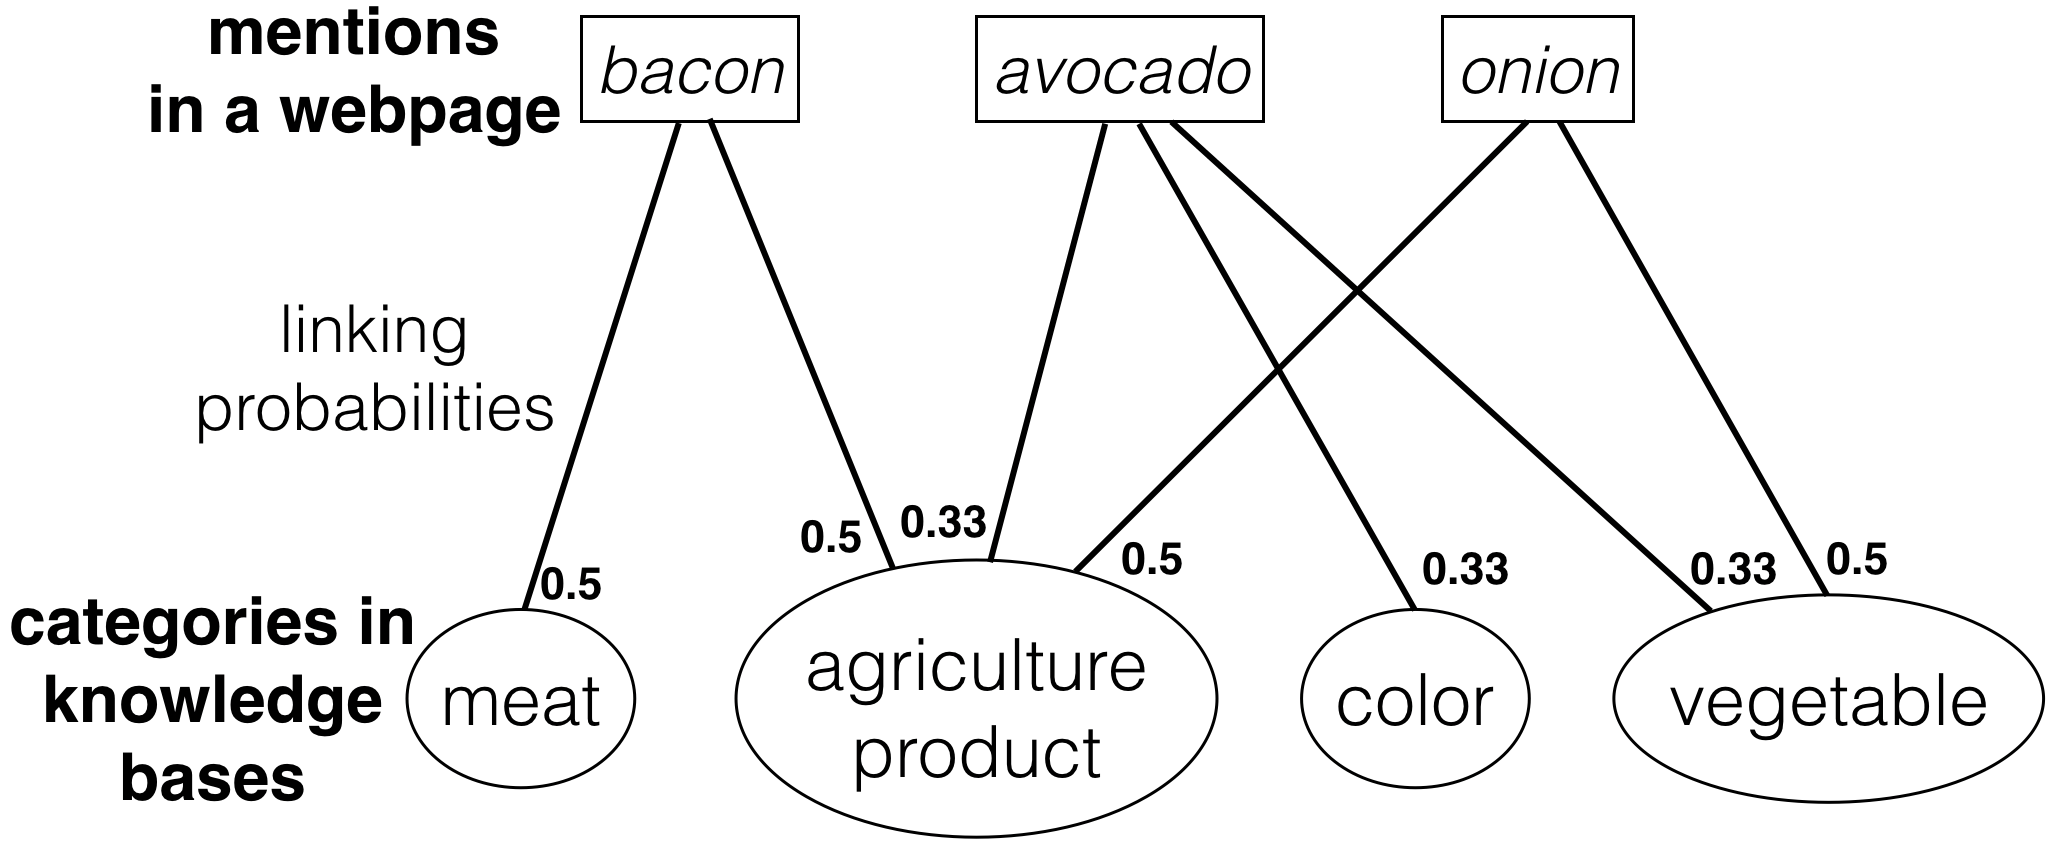
\includegraphics[width=0.5\columnwidth]{Chapters/SearchScape/figures/wsd.png}
    \caption[Word-sense disambiguation in SearchScape.]{When a common noun can be associated with multiple categories due to word-sense ambiguity, SearchScape linked it to all potential categories with uniform linking probabilities.}
    \label{fig:wsd}
\end{figure}


After downloading webpages in the search results, SearchScape analyzes the content to identify potentially useful items and categories. SearchScape generates structures using both content from the webpages in the search results, two external knowledge bases, and two word semantic models. As an overview, words and phrases in the webpages are first linked to concepts in the knowledge bases. We then use the linked concepts and the ontological framework of knowledge bases to infer and rank topical categories in the knowledge bases (such as \emph{GeographicLocations} or \emph{AgricultureProducts}). Finally, we expand the top categories using the word semantic models to ensure good coverage over the search results.

\subsubsection{Linking Mentions to Knowledge Base Concepts}

Linking entity mentions in free text to concepts in knowledge bases and ontologies is a well researched problem in the field of natural language processing known as entity link (for named entities) and word sense disambiguation (for common nouns). SearchScape uses the open source AIDA algorithm to link named entity mentions in the search results to concepts in the Freebase knowledge base \cite{yosef2011aida,bollacker2008freebase}, covering concepts such as \emph{Banff National Park} and \emph{Yosemite National Park}.
For each named entity mention, the AIDA algorithm reports the linking probability of possible concepts in Freebase.
To link common nouns such as \emph{avocados} or \emph{bacon}, we link each word in the search results to all of their possible concepts in NELL with a uniform probability distribution.
For example, the term ``avocado'' can refer to three NELL\cite{carlson2010toward} entities of categories \emph{AricultureProducts}, \emph{colors}, and \emph{vegetables}, respectively (Figure~\ref{fig:wsd}), and SearchScape links ``avocado'' to each of the three concepts with 0.33 probability.
In the next subsection, we describe how we identify the most useful categories based on these linking probabilities using a class-based word-sense disambiguation approach similar to \cite{yarowsky1995unsupervised,chang2009wikisense}.

%Figuring out which category is more useful for the searchers is crucial. Further, since each concept can be listed under multiple categories in a knowledge base, it can still be challenging to identify the most useful category even with the correct mappings between phrases and concepts. For example, ``Banff National Park'' is listed under both \emph{National Parks of Canada} and \emph{Protected areas established in the 19th century} categories in the Freebase knowledge base.


\subsubsection{Topic Inference and Category Ranking}

To identify the most commonly used categories in the search results, SearchScape used a probabilistic model based on the linking probabilities of both named entities and common nouns. The fundamental assumption here is that webpages from the same search result will likely mention concepts of the same categories.
Similar assumptions were found to be effective in past work for word-sense disambiguation \cite{yarowsky1995unsupervised}.
For example, when multiple results for ``guacamole recipes'' mentioned ``avocado'', 
SearchScape uses mentions of different \emph{AgricultureProducts} in the search results to determine
its likely that all avocado mentions were referring to cooking ingredients (\emph{AgricultureProducts}) rather than \emph{colors} or a mix of the two (Figure~\ref{fig:wsd}).
More specifically, it used the linking probabilities to vote on the categories in the knowledge bases. To account for the relevance of a search result based on its position in the ranked list, we weighted the linking probabilities by the reciprocal rank of their sources when voting.

\begin{gather*}
Votes_{category,results} =
\sum_{\substack{entity \in category \\ webpage \in results\\ mention \in webpage}} \
\frac{linkP_{mention,entity}}{rank_{webpage,results}}
\end{gather*}


For example, if ``avocado'' is mentioned in the fourth document, and was linked to three categories each with a probability of $linkP = 0.33$, each of the three categories receives $linkP/rank = 0.33/4 = 0.083$ votes. The total number of votes for a category given a ranked search result list is therefore the sum of linking probabilities to all entities in the category, weighted by the reciprocal ranks of the webpages that mentioned the entities.


%One fundamental assumption here is that the same phrases in sources from the same query always refer to a single concept; that is, all mentions of ``avocado'' in sources of the search results for \emph{guacamole recipes} either refer to an \emph{AgricultureProduct} or a \emph{Color} in NELL. A similar assumption was found to be effective for unsupervised word-sense disambiguation in a different scenario \cite{yarowsky1995unsupervised}. Under this model, the aggregated category scores can in turn be used to re-estimate the linking probability between phrases and concepts using an Expectation-Maximization algorithm (detailed in \cite{yarowsky1995unsupervised}).
%To give some intuition, the model first assigns more weight to a category when many its potential were mentioned in the search results, and in turn assigns higher probabilities to the concepts in categories with higher scores. For example, if there are many more agriculture products in the search results, such as onion, lime, and bacon, comparing to different types of colors, the category agriculture products will be assigned higher scores, and the model will in turn estimate that avocado mentions are more referring to an agriculture products then a colors.
%For simplicity and efficiency, the version of SearchScape presented here only uses the initial score to select the top-1 category for each query, and presents the searcher with a list of its concepts that are mentioned in the search results. This assumption often worked out well in practice, for example identifying travel destinations for the task on Barcelona day trips and ingredients (AgriculturalProduct) for the guacamole recipe task. However, we have also explored a more general version in which people can select different categories to see the distribution of entities from which may be a fruitful topic for future study.
%We also used the same model to rank both NELL and Freebase categories by assigning a linking probability of 1.0 to mappings produced by the AIDA algorithm \cite{yosef2011aida}, since the AIDA algorithm can reportedly produce precise mappings for Freebase entities at around 90\% accuracy \cite{nguyen2014aida}.

\subsubsection{Expanding Coverage}

Knowledge bases can provide high quality ontological information. For example, the Freebase knowledge base defines \emph{Sitges} as a \emph{MunicipalCitiesInBarcelona} and a \emph{GeographicLocations}. However, the coverage of categories over its entities can still be sparse, especially for general categories that can contain up to millions of entities such as \emph{GeographicLocations} or \emph{Person}.
On the other hand, unsupervised word vector models that automatically project words and phrases onto semantic vector spaces to measure semantic similarity can yield high coverage over common words and phrases due to their capacity to train on large, unlabeled corpora \cite{mikolov2013efficient,pennington2014glove}.
%However, in a preliminary study where we clustered frequently mentioned words and phrases using such models, we found that the automatically generated clusters were incoherent and difficult to comprehend by human searchers, even though they yielded good coverage over words and phrases in the search results, a finding which has been echoed by previous researchers \cite{hearst2006clustering,chuang2012interpretation,alloy}.
To take advantage of both the quality of structures in knowledge bases and the coverage of semantic word vector models, SearchScape first use the knowledge bases to identify useful categories as described above. Then, for each category extracted, SearchScape searches the word vector models with the identified key items for semantically similar phrases to add to the category and expand its coverage. 
For example, when a searcher queried SearchScape with ``\emph{day trips from Barcelona}'', SearchScape first identified a list of \emph{GeographicLocations} including \emph{Sitges}, \emph{Girona}, and \emph{Tarragona} from Freebase. To expand the coverage of the \emph{GeographicLocations} category, SearchScape searches the semantic vector space for phrases similar to the already identified key items, and add these similar phrases to the \emph{GeographicLocations} category to expand its coverage. To expand NELL categories that contain mostly common nouns, we used a GloVe model trained on the Common Crawl corpus with 42 billion words and a vocabulary size of 1.9 millions.\footnote{Pre-trained GloVe model downloaded from https://nlp.stanford.edu/projects/glove/} To expand Freebase categories that contain mostly proper nouns, we used a Word2Vec model trained on a news corpus with 100 billion words and a vocabulary size of 1.4 million Freebase entities.\footnote{Pre-trained Word2Vec model downloaded from https://code.google.com/archive/p/word2vec/}

\subsubsection{Hand-off to the Front-end Interface}


Finally, the back-end delivers the following data objects to the front-end interface (Figure~\ref{fig:ds}):

\begin{figure}
    \centering
    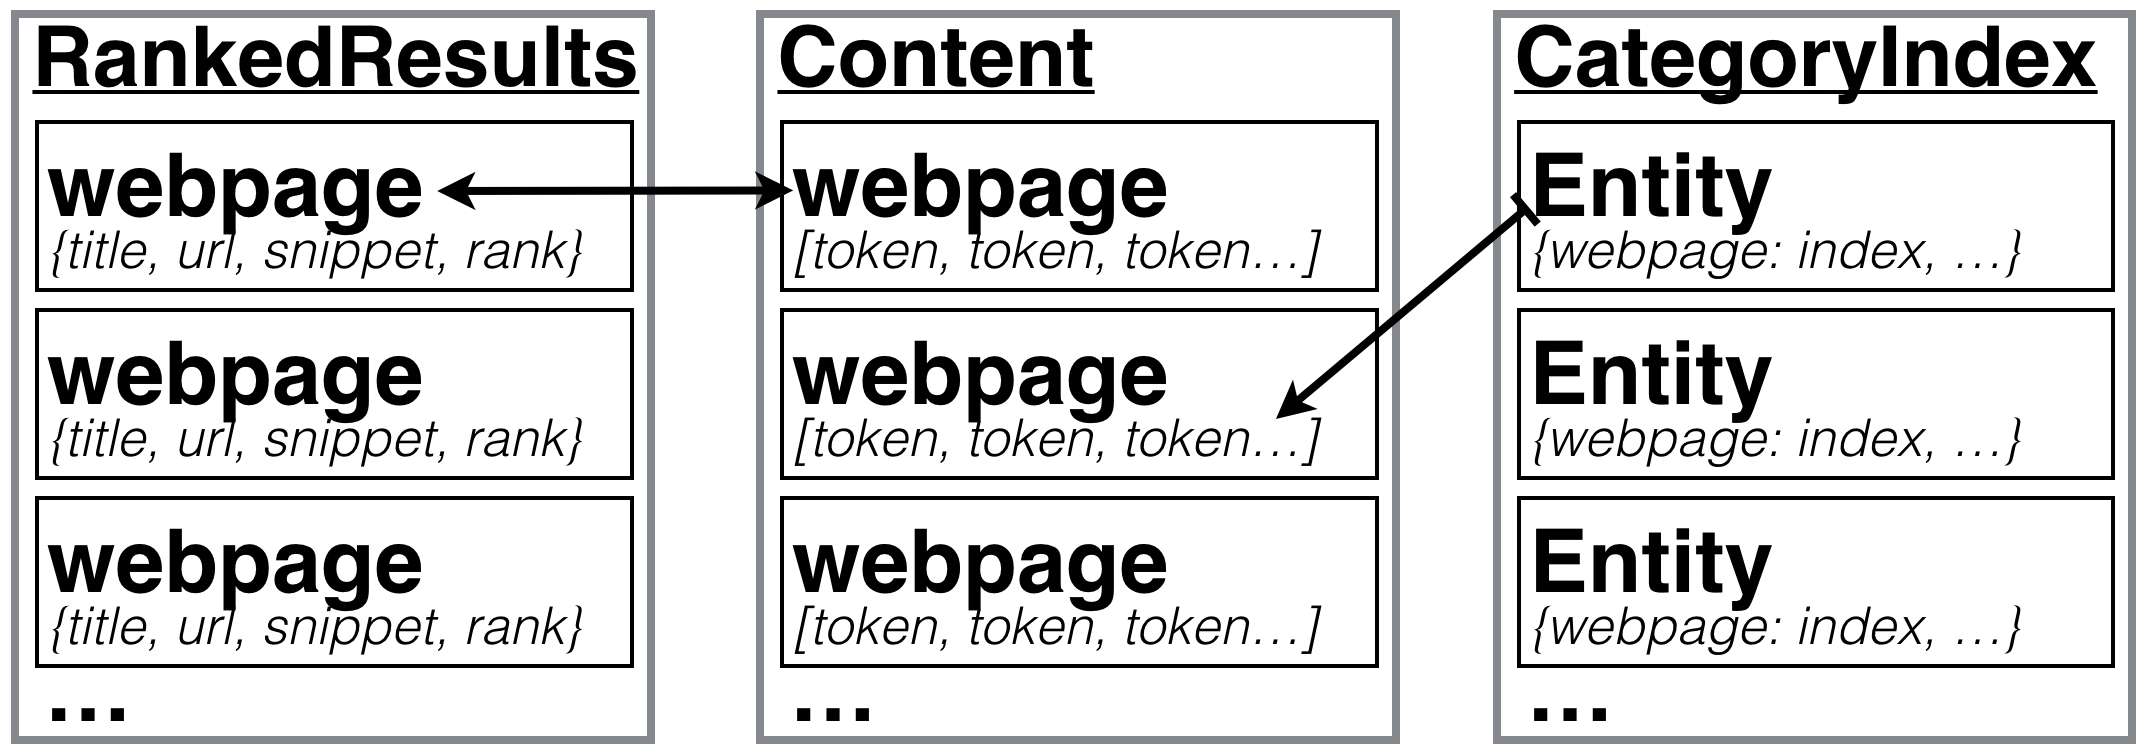
\includegraphics[width=0.5\columnwidth]{Chapters/SearchScape/figures/ds.png}
    \caption[The three data objects produced in the SearchScape back-end component.]{The three data objects produced in the SearchScape back-end component, and passed to its front-end component to enable interactive information exploration. The arrows show the mapping relations between elements in different object.}
    \label{fig:ds}
\end{figure}


\begin{enumerate}
   
    \item \textbf{RankedResults}. The ranked search results retrieved from the Microsoft Bing Web Search API, containing the top 50 results for the given query. Each result contains the rank, URL, title, and a short text snippet from the webpage. 
    
    \item \textbf{WebpageContent}. An index that contains an array of tokenized main content of each webpage in the search results.
    
    \item \textbf{CategoryIndex}. The identified category and its list of entities as described in the previous subsections. Each entity has an inverted-index file\cite{baeza1999modern} of webpages and indices of where the entity was mentioned in WebpageContent. 
\end{enumerate}

Figure~\ref{fig:ds} shows the mapping relations between the three data objects. The addition of CategoryIndex and WebpageContent to traditional web search engines enabled the SearchScape front-end to perform the following complex associations in real-time: 

\begin{itemize}

    \item Filter the RankedResults by using the CategoryIndex to find the list of webpages that mentioned a specific entity of interest, and calculate its proportion of mentions.
%    \item Calculate the proportion of webpages in RankedResults that mentioned a specific entity of interest by counting the length of the filtered RankedResults and its original length.
    \item List sentences that mentioned a specific entity of interest by using the CategoryIndex to find webpages and token indices where the entity was mentioned, and extract sentences from WebpageContent.
    \item Count word frequencies in the extracted sentences to find keywords that frequently co-occur with the entity of interest.
\end{itemize}

We will describe in detail how the SearchScape interface utilize these operations to enable interactive data exploration in the next subsection. 


\begin{figure}
    \centering
    \frame{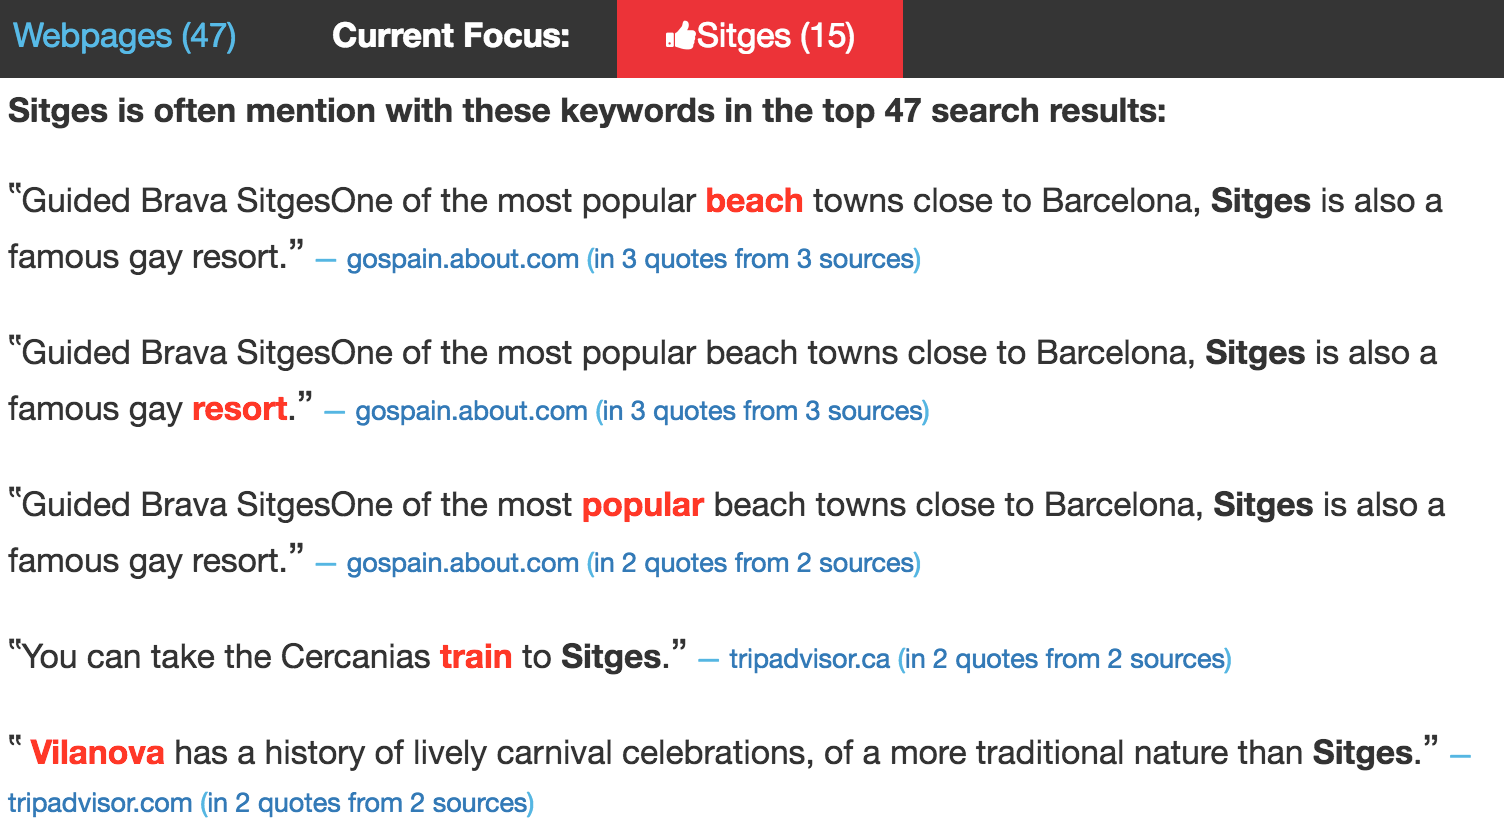
\includegraphics[width=0.6\columnwidth]{Chapters/SearchScape/figures/keywords.png}}

    \vspace{0.5mm}
    
    \frame{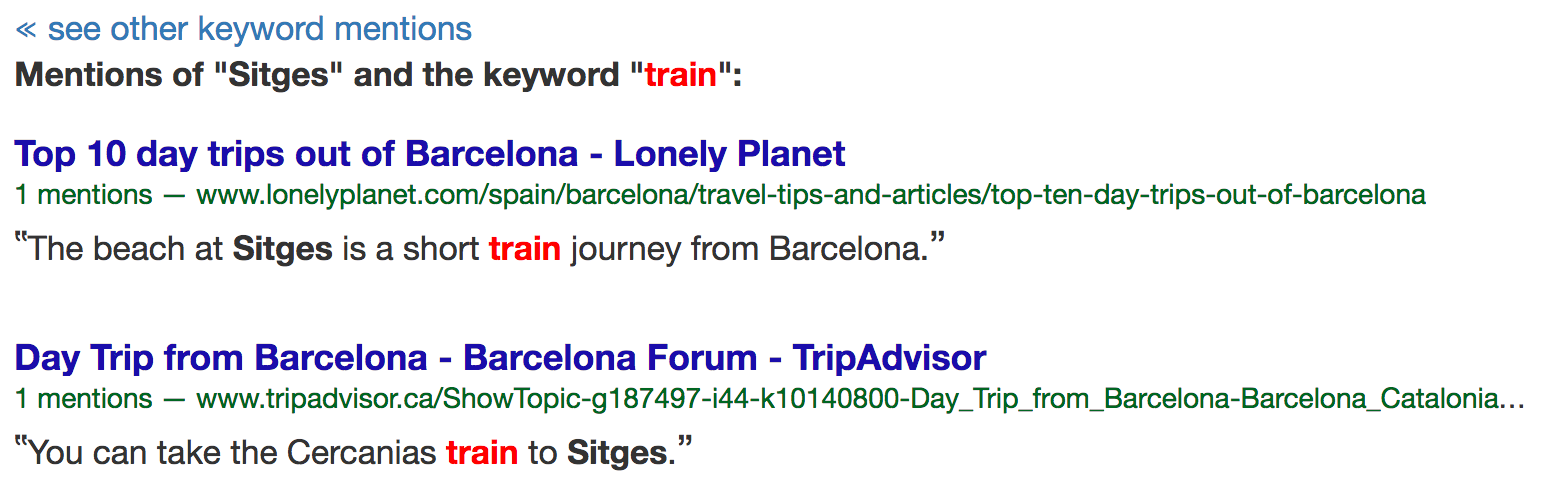
\includegraphics[width=0.6\columnwidth]{Chapters/SearchScape/figures/keywords2.png}}
    
    \caption[Explore mentions and frequently co-occurring words of an concept.]{The searcher clicked on ``Sitges'' from the result page of ``\emph{day trips from Barcelona}'' to explore its mentions grouped by frequently co-occurring keywords, such as \emph{beach}, \emph{resort}, and \emph{train}.}
    \label{fig:keywords}
\end{figure}



\subsection{Interactive Search Landscape}

Using the structures identified by its back-end components, the SearchScape interactive front-end interface augments traditional ranked list search results both to provide a quick overview of the information landscape, and to enable deep user interaction for exploring important subtopics specific to the current query. 

%
%\begin{figure}
%    \centering
%    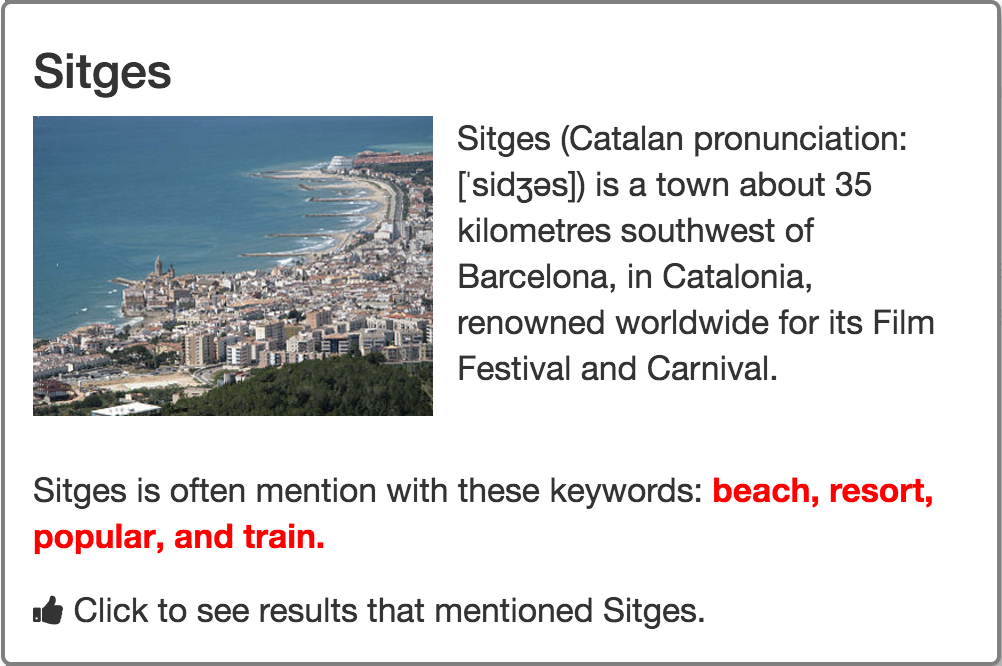
\includegraphics[width=0.6\columnwidth]{Chapters/SearchScape/figures/preview.png}
%    \caption{Hovering over an extracted item in SearchScape allows searchers to read a short definition of the concept and frequently co-occurring keywords. Here, the searcher hovered over ``Sitges'' from the search result page of ``\emph{day trips from Barcelona}''.}
%    \label{fig:preview}
%\end{figure}


SearchScape supports many key tasks defined in Shneiderman's task taxonomy of information visualization \cite{shneiderman1996eyes}, such as \emph{overview}, \emph{zoom}, \emph{filter}, and \emph{details-on-demand}. The interface consists of a Structure Panel on the left, and a Document Panel on the right (Figure~\ref{fig:flow}, left). When a new search results is loaded, the Structure Panel on the left displays an \emph{overview} of the current information space using the distribution information of items in the identified category, and the Document Panel on the right lists webpages in the search results. Similar to many commercial search engines, the Document Panel shows the title, URL, and a short snippet related to the query terms for each webpage in the search results. Even though SearchScape can automatically identify key concepts from the search results, exploratory searchers might not be familiar with the extracted concepts, especially in early stages of the exploratory search process. Therefore, SearchScape allows searchers to \emph{demand-for-details} when needed by hovering over the items to see short descriptions of the concepts from external knowledge bases (Figure~\ref{fig:flow}, left). In addition, SearchScape also extracts a list of keywords that frequently co-occur with the concept of interest in the search results using the inverted-index file. When the searchers discovered an interesting item, they can \emph{filter} the Document Panel by clicking the item of interest (Figure~\ref{fig:filter}, left). A focus tab will appear on the top of the Document Panel to indicate the the current items of interest (Figure~\ref{fig:filter}, center), and the Document Panel will re-rank webpages that mentioned the item to the top of the list, as well as update the short descriptions to show parts of each webpage that mentioned the item. Instead of looking through the filtered search result list, searchers also have the option to \emph{zoom-in} to the current focused item by clicking on the focus tab to see sentences in the search results that mentioned the item of interest, grouped by frequently co-occurred keywords (Figure~\ref{fig:keywords}).

\begin{figure}
    \centering
    \frame{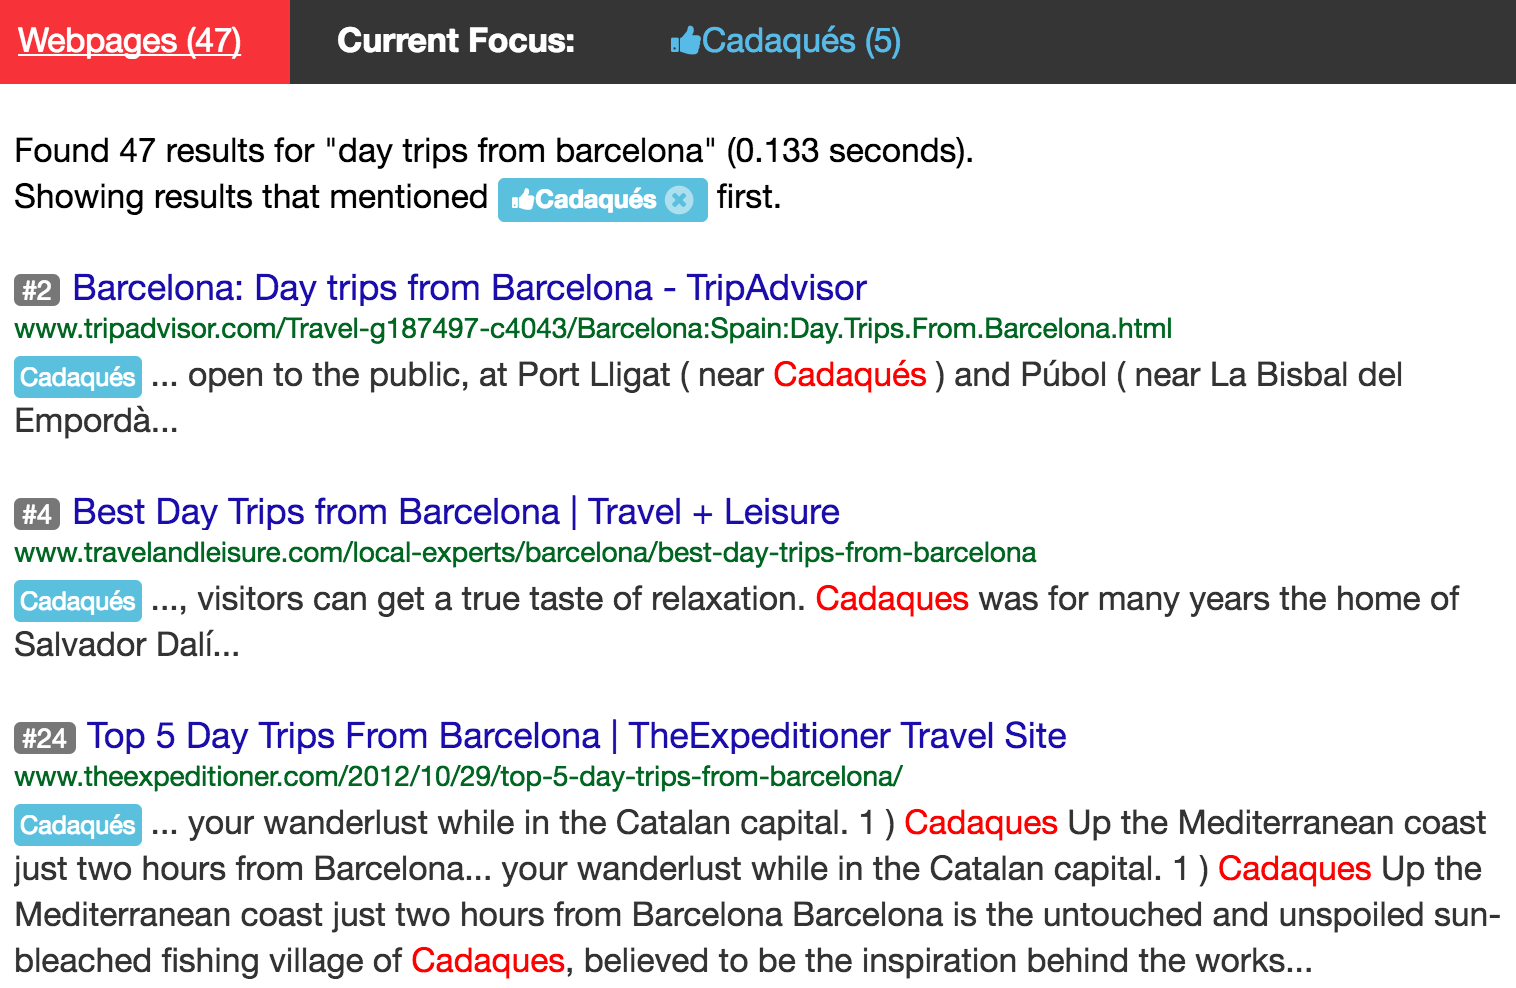
\includegraphics[width=0.6\columnwidth]{Chapters/SearchScape/figures/filter.png}}
    \caption[Filtering the search results using ``Cadaqu\'es'' from the result page.]{The searcher filtered the search results using ``Cadaqu\'es'' from the result page of ``\emph{day trips from Barcelona}''. Notice the snippets are updated to show relevant parts of each webpage.}
    \label{fig:filter}
\end{figure}


To give a sense of how an exploratory searcher might use SearchScape, we will use Figure~\ref{fig:flow} as an example scenario. In our scenario, the user searched for ``\emph{day trips from Barcelona}'', the SearchScape back-end analyzed sources in the search results and identified the Freebase category \emph{GeographicLocations} as the most useful category for the current task. The list of ranked search results are presented to the user in the Document Panel, and a list of different destinations and how frequently each of them are mentioned by different sources are presented in the Structure Panel. By examining the items in the \emph{GeographicLocations} category, the user quickly gained an overview of how many different destinations are in the search results, and how popular each of the choices are (Figure~\ref{fig:flow}, left). The user then proceeded to explore the different choices in the Structure Panel by hovering over each of the items. The user noticed that the destination ``Sitges'' is mentioned in a third of the sources, and is also frequently mentioned with keywords that matched with his or her interests, such as ``\emph{beach}'' and ``\emph{resort}''. To access more information about Sitges, the user clicked on Sitges to surface sources that mentioned Sitges (Figure~\ref{fig:flow}, center. Figure~\ref{fig:filter}), and also directly explored sentences from different sources that mentioned both ``Sitges'' and ``beach'' (Figure~\ref{fig:flow}, right. Figure~\ref{fig:keywords}).


\section{Evaluation}



We evaluated SearchScape through two studies aimed at assessing the coherence of the identified structures and the usefulness of the interface, respectively. For the first study, we compared structures generated for 50 different search queries from an exploratory search database \cite{potthast2013exploratory,Hagen:2016:WSA:2854946.2854969} using both SearchScape and Carrot2 \cite{stefanowski2003carrot}, a search result clustering system.
For the second study, we recruited 210 unique participants from Amazon Mechanical Turk for a user study \cite{kittur2008crowdsourcing}.
Three diverse search scenarios were designed as between-subject conditions in Study 2 to evaluate the usefulness and generalizability of SearchScape. 
To further examine whether providing distribution information is actually beneficial to searchers,
we grouped participants under each of search scenario into two front-end conditions to test the effects of hiding and exposing distribution information of the extracted items (Figure~\ref{fig:conds}). In the following subsections, we will describe the two studies in detail.

\begin{figure}
    \centering
    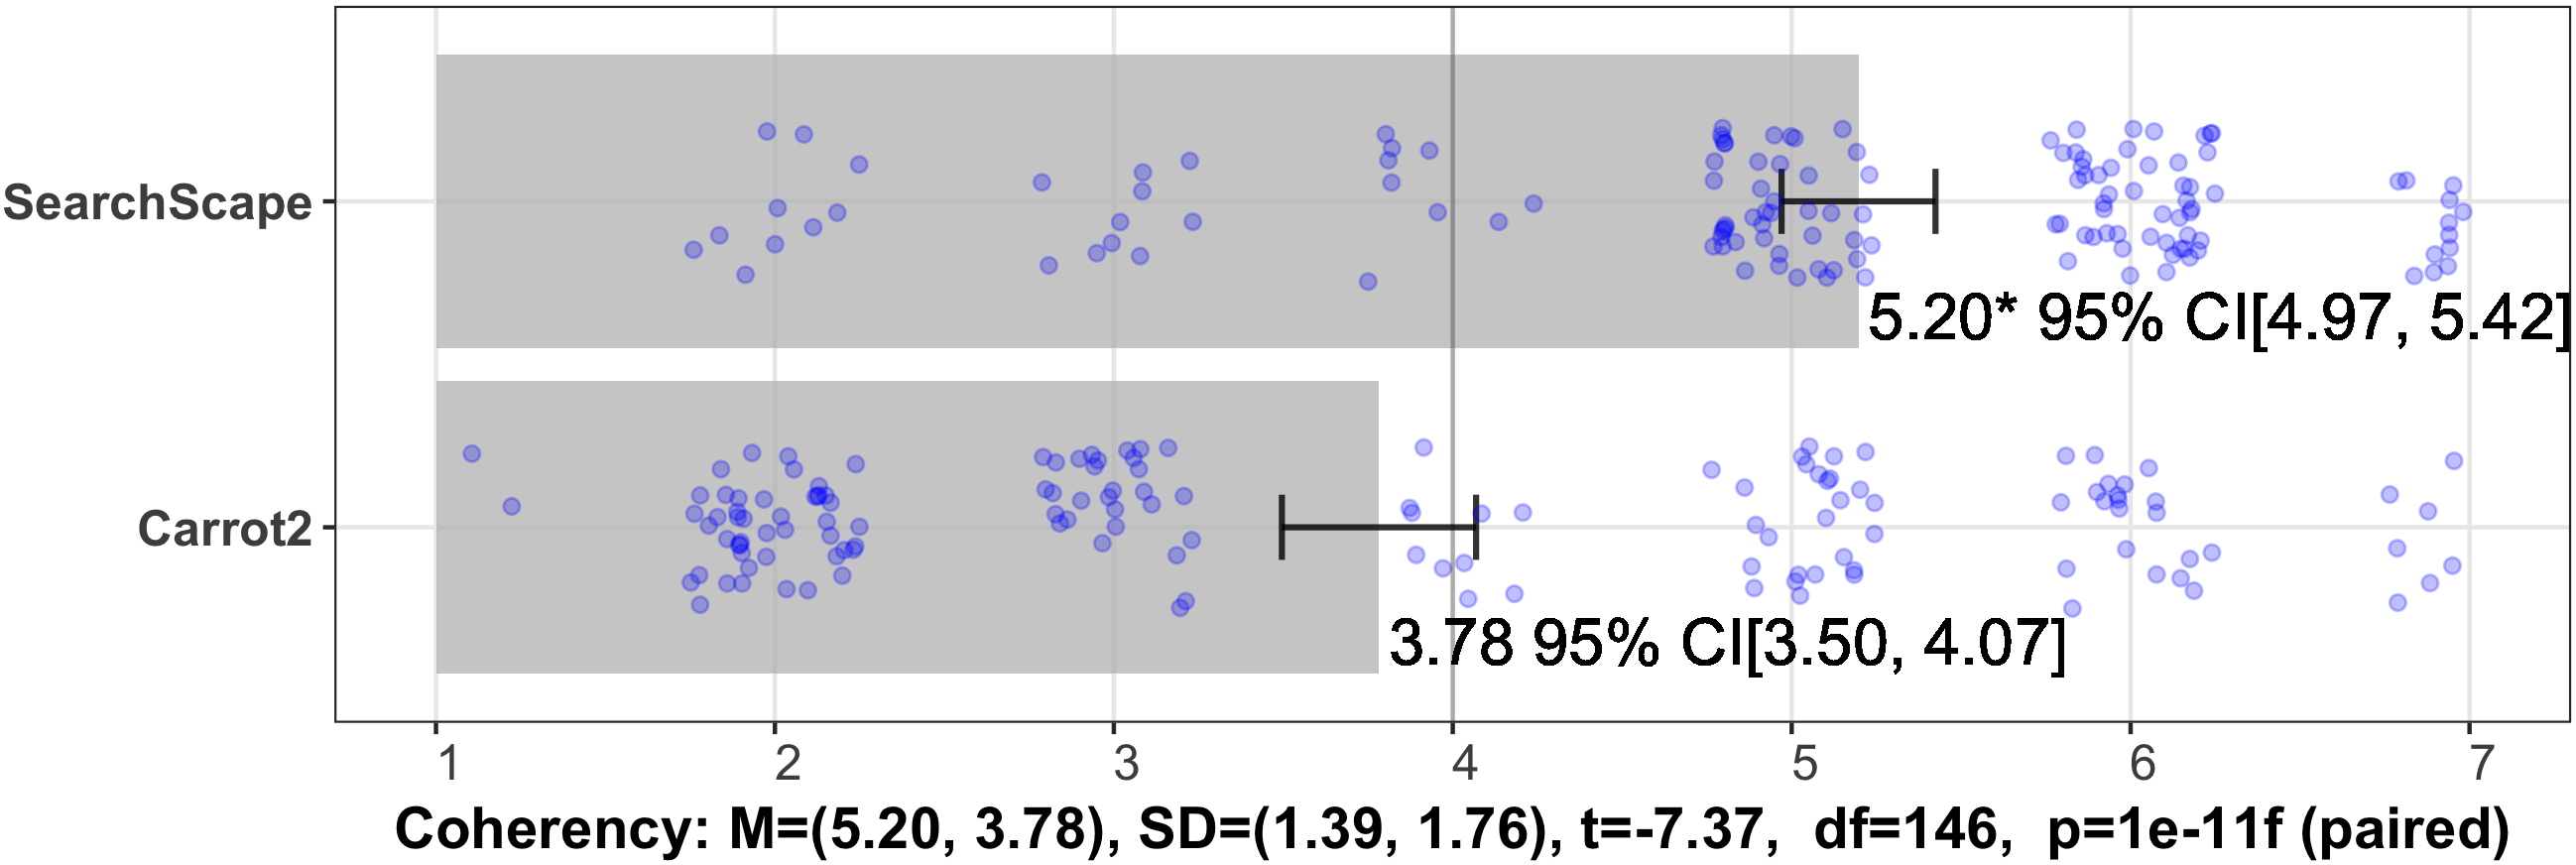
\includegraphics[width=0.6\columnwidth]{Chapters/SearchScape/figures/coherence_label.png}
    \caption[SearchScape structures were found to be strongly coherent, and significantly more coherent compared to Carrot2 based on paired t-test.]{Using 7-point Likert scales,  
    SearchScape structures were found to be strongly coherent (M=5.20*, 95\% CI[4.97, 5.42]), and significantly more coherent compared to Carrot2 (M=3.78*, 95\% CI[3.50, 4.07]) based on paired t-test (N=147, t=-7.37, df=146, p<0.001). The error bars indicate confidence intervals.
        }
    \label{fig:coherence}
\end{figure}

\begin{table}
\small
    \centering
    \begin{tabular}{l}
    \hline
        Statements \\
        \hline
        
        S1. Seeing the \textbf{list of items} on the left is useful \\
       
        S2. The \textbf{distribution/rank} each item is on the left is useful \\
        
        S3. Clicking on an item to see \textbf{webpages} that \textbf{mentioned} it is useful \\
        
        S4. Seeing \textbf{keywords} often \textbf{mentioned} together with the items is useful \\
        
        S5. For complex searches, this is an \textbf{improvement} to current interfaces \\
        
        S6. I would \textbf{prefer} it if my search engine have these extra features \\
        
        S7. I think the extra features would help me \textbf{find better} information \\
        
        S8. The interface is a \textbf{distraction} or makes searching more \textbf{stressful} \\
        
        \hline
        
    \end{tabular}
    \caption[Full statements rated by the participants.]{Full statements rated by the participants. Statements were not stylised in the survey.}
    \label{tab:statements}
\end{table}



\begin{table}
\small
    \centering
    \scriptsize
    \begin{tabular}{r | l l | l l | l l}

    & \multicolumn{2}{c|}{Barcelona} & \multicolumn{2}{c|}{Guacamole} & \multicolumn{2}{c}{Guggenheim} \\ 
        Stmt. & DIST & RANK & DIST & RANK & DIST & RANK   \\
        \hline
        
        
        S1 & 
        \textbf{4.35}[4.11, 4.60] & 4.12[3.82, 4.43] &  
        \textbf{3.97}[3.99, 4.66] & 3.86[3.69, 4.42] & 
        4.22[3.88, 4.57]& \textbf{4.36}[4.08, 4.64]\\
        
        S2 &
        \textbf{4.32}[4.02, 4.63]\textsuperscript{\tiny *} & 3.82[3.45, 4.19] &
        3.89[3.45, 4.33] & 3.89[3.53, 4.26]& 
        4.28[3.93, 4.63] & \textbf{4.44}[4.20, 4.69] \\
        
        S3 &
        \textbf{4.19}[3.89, 4.50]& 4.09[3.78, 4.40]&
        \textbf{4.11}[3.70, 4.51]& 4.08[3.69, 4.47]&
        4.28[3.96, 4.60] & 4.28[3.99, 4.57] \\
        
        S4 &
        \textbf{4.39}[4.12, 4.65] & 4.09[3.74, 4.44]&
        \textbf{3.89}[3.42, 4.37]& 3.76[3.35, 4.17]&
        4.03[3.65, 4.40] & 4.03[3.71, 4.35] \\
        
        S5 &
        \textbf{4.19}[3.89, 4.50]\textsuperscript{\tiny **} & 3.52[3.15, 3.88]&
        4.03[3.62, 4.44]& 4.03[3.65, 4.41]&
        3.94[3.54, 4.35] & \textbf{4.17}[3.86, 4.47]\\
        
        S6 &
        \textbf{4.19}[3.87, 4.51]\textsuperscript{\tiny *} & 3.58[3.20, 3.95]& 
        \textbf{3.76}[3.32, 4.20] & 3.46[3.02, 3.89] &
        \textbf{3.83}[3.42, 4.24] & 3.78[3.43, 4.12]\\
        
        S7 &
        \textbf{3.21}[2.84, 3.58]\textsuperscript{\tiny *} & 2.60[2.26, 2.95]&
        \textbf{3.00}[2.59, 3.41]& 2.70[2.32, 3.09]&
        3.03[2.61, 3.45] & 3.03[2.67, 3.38] \\
        
        \hline
        
        \textbf{Aggr.} &
        \textbf{4.15}[4.03, 4.27]\textsuperscript{\tiny ***} & 3.69 [3.55, 3.83]&
        \textbf{3.81}[3.65, 3.97] & 3.68[3.53, 3.84]&
        3.95[3.80, 4.09]& \textbf{4.01}[3.89, 4.14]\\
        
        \hline
        
        S8 &
        \textbf{2.45}[1.92, 2.99] & 2.79[2.35, 3.23]&
        \textbf{2.19}[1.77, 2.61]& 2.49[2.03, 2.94]&
        \textbf{2.28}[1.86, 2.70] & 2.39[1.94, 2.83] \\
        \hline
        
        \textbf{N} & 31 & 33 & 37 & 37 & 36 & 36 \\
        

        
    \end{tabular}
    \caption[Survey responses under different tasks and conditions.]{(Full statements in Table~ \ref{tab:statements}) Survey responses (mean and 95\% confidence interval) under different tasks and conditions using a 5-point Likert scale. A score of 5 indicates strong agreement with the statement, and a score of 1 indicates strong disagreement. Confidence intervals above 3 indicates significant agreement. Asterisks indicate significant differences between conditions under independent t-test.  \textsuperscript{\tiny *}p $\boldsymbol \le$ 0.05,\textsuperscript{\tiny **}p $\boldsymbol \le$ 0.01, \textsuperscript{\tiny ***}p $\boldsymbol \le$ 0.001}
    \label{tab:survey}
\end{table}



\subsection{Study 1: Automatic Structuring}

To evaluate the quality of the structures produced by SearchScape, we compare it against the open source search results clustering system Carrot2 \cite{stefanowski2003carrot}, which produces interpretable names for each of its clusters. To cover a wide variety of search topics and scenarios, we randomly selected 49 queries from different topics found in a exploratory search database that contains a total of 150 search tasks derived from
the TREC Web track topics of the years 2009 to 2011 \cite{Hagen:2016:WSA:2854946.2854969}. The queries are collected from participants conducting exploratory search for the 150 search tasks in a lab setting \cite{potthast2013exploratory}. We submit each of the 49 queries to both SearchScape and Carrot2 and obtained a total of 98 search result structures. Finally, we present each of the task descriptions, queries, and the pair of structures to 3 crowdworkers. For each structure, we asked the crowdworkers to rate the statement ``\emph{Items in the list are of the same type}'' using a 7-point Likert-scale ranging from Strongly Disagree (1) to Strongly Agree (7), and a score of 4 indicates neutral.

        


%comprehensiveness of the identified structures, we manually compiled gold-standard structures for the two exploratory search tasks by reading through the 50 results for each of the two queries and extracting the destinations and ingredients, respectively. We then used the gold-standard labels to evaluate both the precision and recall rate of the SearchScape categories and items. To account for prominence, we weighted the recall rate using the number of results that mentioned each item in the gold-standard labels. 


\subsubsection{Results}


As shown in Figure~\ref{fig:coherence},
participants agreed strongly that SearchScape produced structures that were coherent (M=5.20*, 95\% CI[4.97, 5.42]).
When compared side-by-side against structures produced by Carrot2, crowdworkers rated SearchScape as more coherent (M=(3.78 vs 5.20), SD=(1.76, 1.39)). This difference was significant based on a paired t-test (N=147, t=-7.37, df=146, p=1e-11f < 0.001). The results suggest that for a wide variety of exploratory search scenarios, SearchScape can produce structures more coherent than traditional search result clustering approaches. %In Study 2, we examine if the structures were actually beneficial to searchers using the interactive SearchScape interface. Further, we explore if exposing distribution information with these coherent structures has a positive effect to searchers.

%As shown in Figure~\ref{fig:pr}, for the Barcelona task, SearchScape identified the Freebase \emph{GeographicLocations} category, which initially covered 45\% of the entities in the gold-standard, and has a precision rate of 81\%. Expanding the category using the Word2Vec model raised the recall rate from 45\% to 68\%, and only lowered the precision rate by 1\%. For the Guacamole task, SearchScape identified the NELL \emph{AgriculturalProducts} category, which initially already covered 66\% of the gold-standard labels, but at with a lower precision rate of 64\%.  After expanding the category using the GloVe model, the coverage was further increased to 72\%, but at the cost of decreasing the precision rate to 56\%. In both scenarios, SearchScape reached around 70\% recall rate, which covered the majority of concepts that were mentioned in at least two sources due to long-tail effects (around half of the gold-standard labels were items only mentioned once in the search results). We also examined cases where SearchScape included concepts that were not in the gold-standard, and discovered the main cause being some sources contained information irrelevant to the query. For example, webpages that contained guacamole recipes but also recipes of other dishes, or webpages that contained information about day trips from Barcelona, but also multi-day plans that reached places too far for day trips. 


%\begin{figure}
%    \centering
%    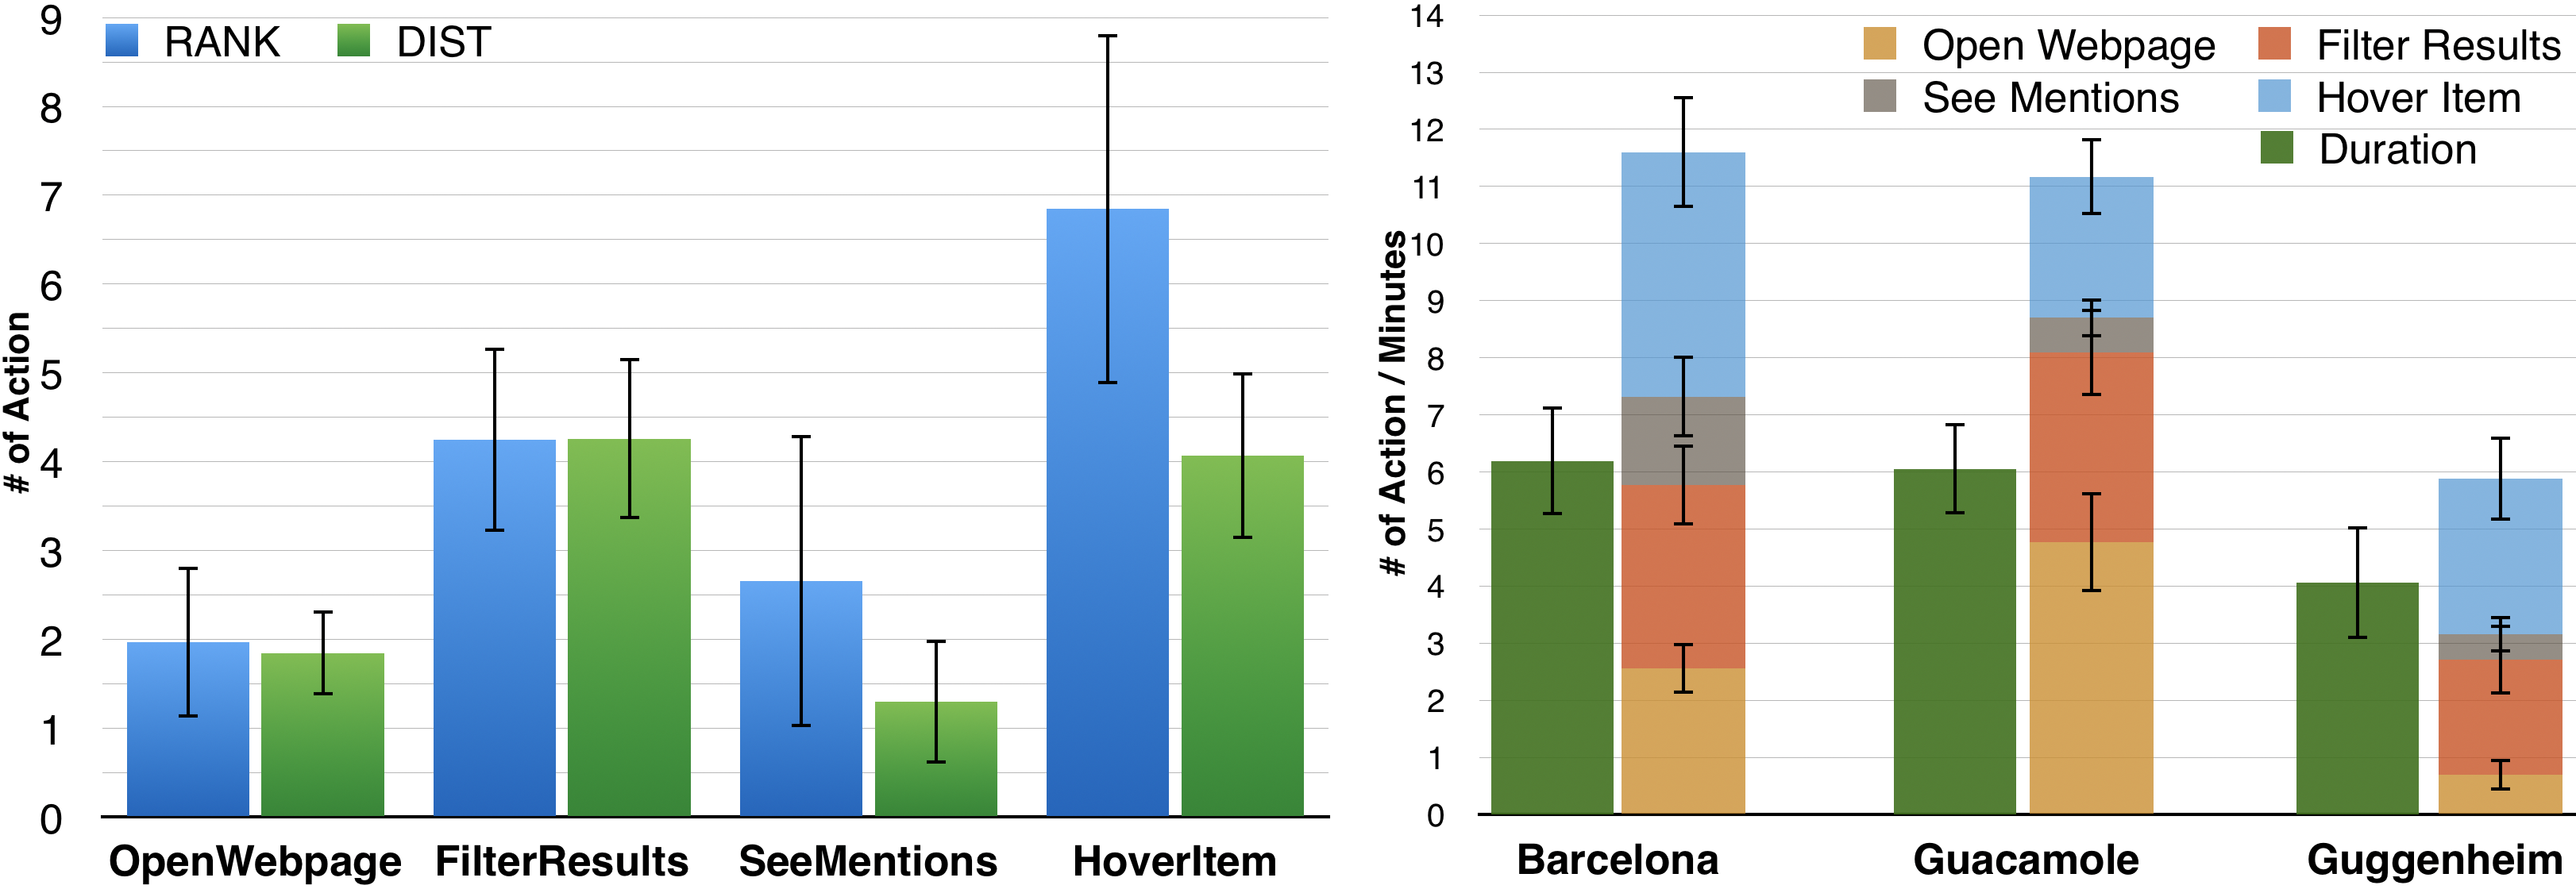
\includegraphics[width=0.96\columnwidth]{Chapters/SearchScape/figures/time.png}
%    \caption{Average number of actions each participant performed in the two exploratory tasks (left). Average number of actions participant performed and average duration spent under different tasks (right).}
%    \label{fig:time}
%\end{figure}


\begin{figure}
    \centering
    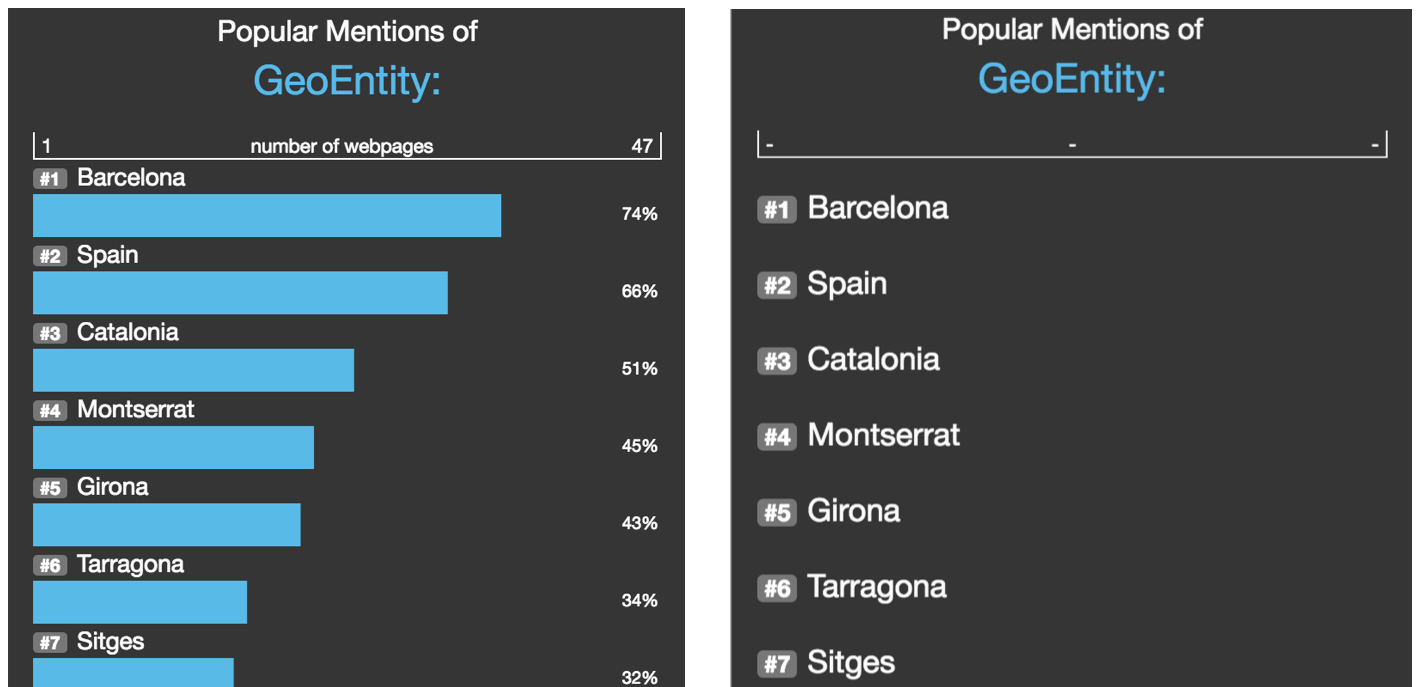
\includegraphics[width=0.6\columnwidth]{Chapters/SearchScape/figures/conds_short.png}
    \caption[A baseline system used in the SearchScape study.]{The DIST condition (left) shows the proportion of results mentioned each items in the category. The RANK condition (right) hides the distribution information, but still shows the ranking of each item.}
    \label{fig:conds}
\end{figure}



\subsection{Study 2: Exploratory Search}

Automatically identifying important structures and displaying distribution information are the two key components that differentiate SearchScape from traditional Web search interfaces and previous work. In order to evaluate the usefulness of the SearchScape interface, and more specifically, the benefits of exposing structural and/or distribution information to searchers, we conducted a user study with 210 unique participants recruited from Amazon Mechanical Turk (age between 18 and 68, M=35, SD=11, 57\% male and 43\% female, mostly from the US) \cite{kittur2008crowdsourcing}.

The experiment was a 3x2 between subjects design, with participants randomized into one of the three different search scenarios and one of the two interface conditions (rank+distribution or rank only) as shown in Figure~\ref{fig:conds}. The \textbf{DIST} condition consisted of all features described in the previous section, which showed both the ranks and proportions of webpage mentions of the items using text labels and horizontal blue bars of different lengths. The \textbf{RANK} condition consisted of all the same interactive features, but hid the distribution of items by only showing their ranking. 
During the study, participants first filled out a pre-survey about their demographic information, we then presented each participant with their assigned search tasks.
%In the first part of the study, we provided the participants with only the top search results of each task without the SearchScape features. For the \textbf{Barcelona} task, we provided the top-1 search results from the Bing Web Search API, which contains seven day trip destinations from Barcelona.\footnote{touropia - 7 Great Day Trips from Barcelona, http://www.touropia.com/day-trips-from-barcelona/} For the \textbf{Guggenheim} task, we also provided the top-1 search result, which contains the correct answer in the second paragraph.\footnote{Wikipedia - Solomon R. Guggenheim Museum, https://en.wikipedia.org/wiki/Solomon\_R.\_Guggenheim\_Museum} For the \textbf{Guacamole} task, we provided the top-7 search results, which, in total, contains seven recipes. We asked the participants to review top results and answer the tasks the best they can. This part of the study aimed to ensure that they are aware of the uncertainty in the tasks (i.e., multiple choices exist), and motivate them to verify and explore different the options in the next part of the study \cite{kules2008creating}. In the second part of the study, 
They then watched a 70 second video tutorial introducing the features of SearchScape according to their front-end conditions. They were then asked to conduct the assigned search tasks using SearchScape. As they interact with the interface, we recorded their actions for further analysis. Finally, we collected their opinions about SearchScape in a post-survey (Table \ref{tab:survey}). 

\subsubsection{Search Scenarios}

Creating tasks to effectively evaluate exploratory search systems is itself a challenging task \cite{kules2008creating,white2006report}. Challenges include finding topics that are unfamiliar yet still relatable for the participants and motivating participants to explore and evaluate different options. We designed two exploratory tasks of different complexity, following the task design suggestions outlined in \cite{kules2008creating}, such as providing ample imaginative context, and being specific about the information necessary for their assigned search task. In addition, we also included one fact-finding task to see if the additional features of our interface would interfere or cause annoyance in non-exploratory scenarios. For each task, participants were given a fixed query that we have fetched and indexed in advance using the back-end of SearchScape. Below are the three tasks we utilized in this study and their corresponding queries:

\begin{itemize}
    \setlength\itemsep{0.0em}
    \item \textbf{Barcelona}. ``\emph{You have a friend who's planning a day trip from Barcelona, and you want to help her figure out 3 destinations that you considered the best options. Give a short explanation about why you picked each of the destinations.}'' \textbf{Query}: ``\emph{day trips from Barcelona}''
    \item \textbf{Guacamole}: ``\emph{You are in charge of making guacamole for a party you and your friends are hosting. You've decided to do some searching online to find 3 recipes you like the most.  Give a short explanation about why you picked each of the recipes.}'' \textbf{Query}: ``\emph{guacamole recipes}''
    \item \textbf{Guggenheim}: ``\emph{You need to find out who designed The Guggenheim Museum in New York City for a school report, and you decided to search the Internet for the answer. Give a short explanation for how you found the answer.}'' \textbf{Query}: ``\emph{who designed the Guggenheim Museum?}''
\end{itemize}

The three tasks were designed with the following factors in mind. The \textbf{Barcelona} scenario promotes objective decision making based on the information presented, since we did not specify a persona for the person participants were gathering information for. Conversely, the \textbf{Guacamole} scenario promotes subjective decision making, since the participants are searching for recipes for themselves.
%We therefore expected participants to benefit more from the distribution information in the first task, and hope the overview provided by the structures can help participants to find unique options that they preferred.
In addition, the relationship between the identified structures and information needs also differs. SearchScape identified a list of \emph{geographic locations} for the \textbf{Barcelona} query, which were mostly competing \emph{places} for day trip destinations, whereas for the \textbf{Guacamole} query, SearchScape identified \emph{agriculture products}, which contained mostly composable \emph{ingredients} of different recipes.
%We considered the \textbf{Barcelona} task to be our most complex task, containing unfamiliar choices with multiple attributes (i.e., activities for different destinations), and expected most participants to actively engage in exploratory search during the study. On the other hand, \textbf{Guacamole} task was designed to be a simpler exploratory task, where participants were likely already familiar with the ingredients of different recipes before the study.
Finally, we included the simple fact-finding \textbf{Guggenheim} task to see if participants find the extra features overwhelming or detrimental for finding a single correct answer.

\begin{figure}
    \centering
    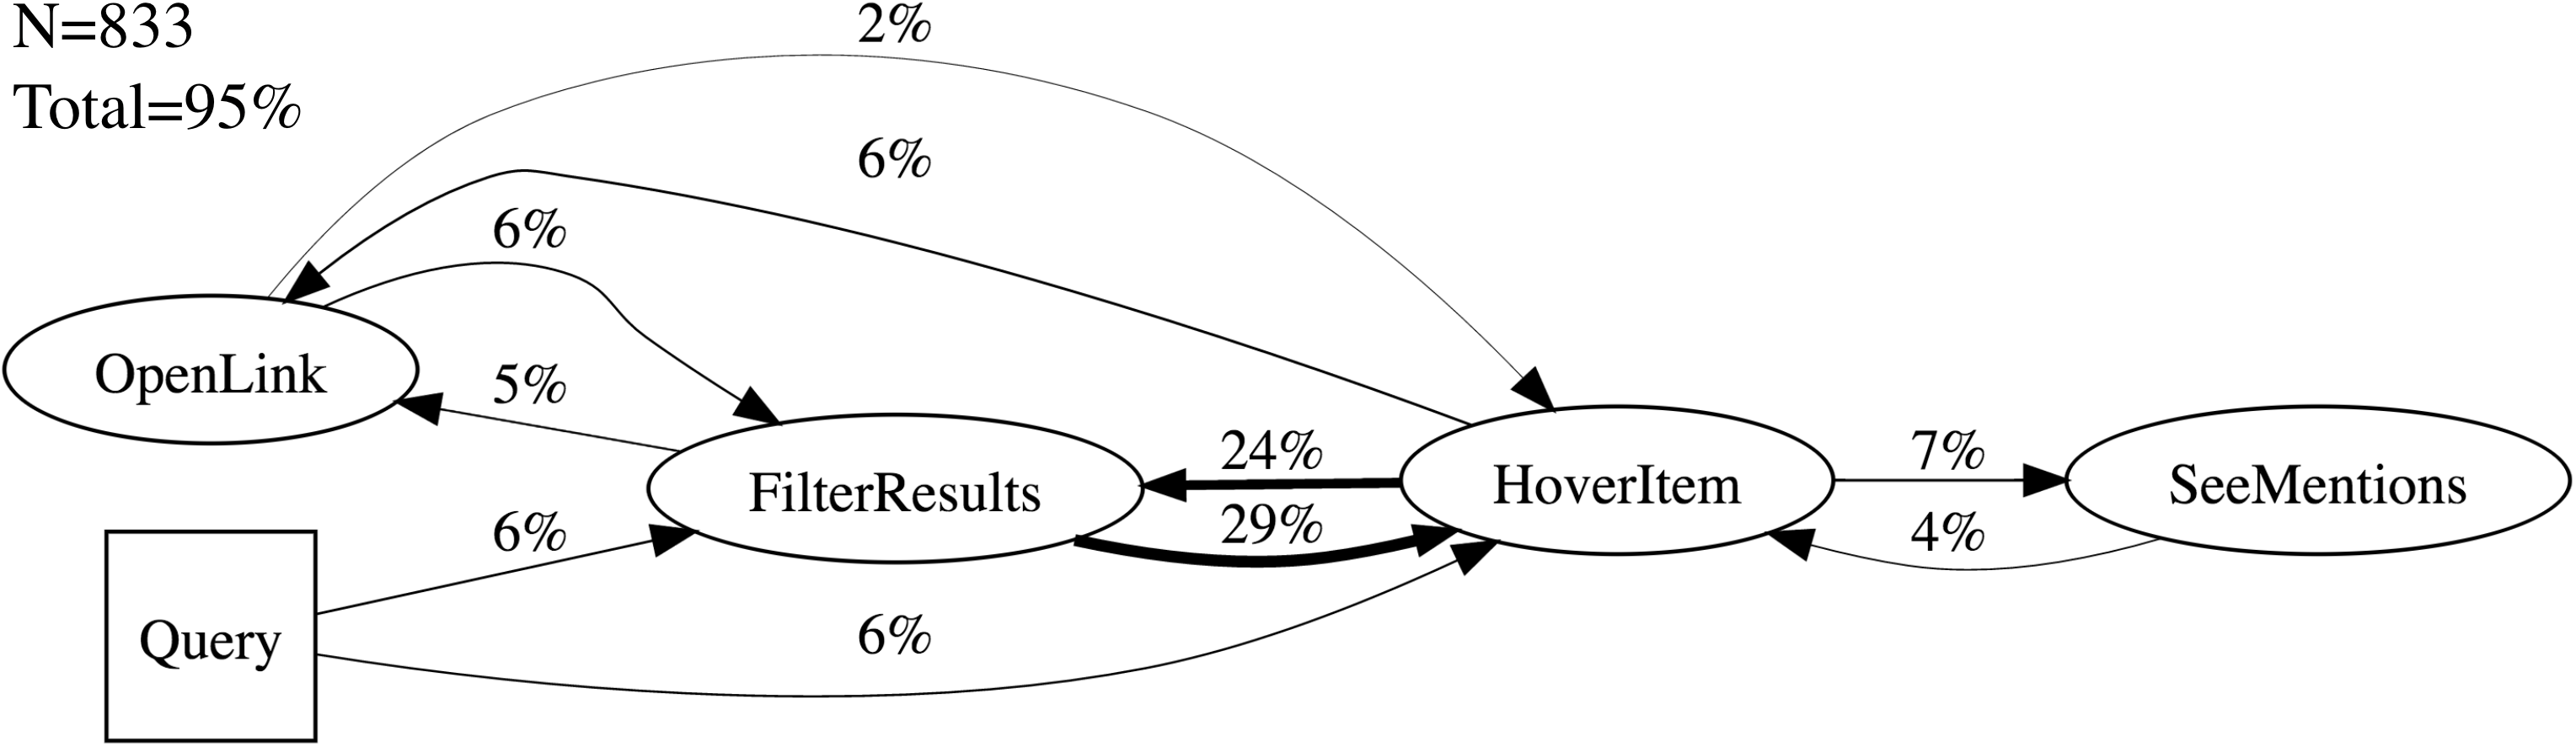
\includegraphics[width=0.7\columnwidth]{Chapters/SearchScape/figures/trans.png}
    \caption[Top transitions between different features.]{Top transitions between different features of participants across all conditions.  Around half of the participants started by hovering items, while the other half by filtering the search results.}
    \label{fig:trans}
\end{figure}


\section{Results and Discussion}


\subsection{Behavior}

%On average, participants performed 11.5 actions in 6 minutes for the two exploratory tasks, and 6 actions in 4 minutes for the fact-finding task (Figure~\ref{fig:time}).
%Participants were also actively engaged with the features provided by SearchScape (Figure~\ref{fig:time}, left).
%On average, participants in the RANK condition performed more HoverItem and SeeMentions actions, but the differences were not significant. 
%Participants also used the structures to gain an overview of the information space. 
SearchScape augments traditional search interfaces with a interactive information landscape. First, we examine whether participants were actually using the added features. 
Figure~\ref{fig:trans} shows the top 10 transitions between different SearchScape features, and
participants almost always explored the overview information in the Structure Panel first, instead of opening links from the list of search results directly. Similar findings have been reported in previous work on using a faceted interface to explore a library catalog \cite{kules2009exploratory}.


% \subsubsection{Results: Searcher Preferences}
% Table \ref{tab:survey} shows the eight survey questions and responses we collected. The first four questions were each about a different feature of SearchScape. The next three questions were about their overall opinions about SearchScape, including two questions comparing SearchScape to traditional web search interfaces. Finally, we asked the participants whether the additional features of SearchScape caused distractions or stress. In general, participants responded favorably to both SearchScape conditions, even in the fact-finding \textbf{Guggenheim} task. Comparing the two frond-end conditions, the DIST condition were found to be significantly more useful than the RANK condition, but only in the most complex \textbf{Barcelona} task. Finally, we also coded the answers and general feedback from participants, and we will show representing quotes in the Discussion Section.


\subsection{SearchScape vs Traditional Web Search Interface}

SearchScape augments traditional web search interfaces with structure and distribution information, which enables interactive information exploration. The results of our studies suggested the structure and distribution information helped participants process and navigate large amounts of information efficiently.
Participants were asked to compare SearchScape to their current search engine interfaces using a 5-point Likert scale (Table \ref{tab:survey}, DIST condition). Across three search tasks, participants generally agreed that SearchScape is an improvement to current interfaces (average: 4.2*, 4.0*, 4.0*, respectively, 95\% CI > 3.0), and would prefer it if their search engines also had the extra features (average: 4.2*, 3.8*, 3.8*, respectively, 95\% CI > 3.0). Further, they also agreed that the added features did not cause distraction or stress, even for the fact-finding Guggenheim task (average: 2.5*, 2.2*, 2.3*, respectively, 95\% CI < 3.0). In the general feedback, participants also expressed how SearchScape is an improvement to the current interfaces, and how they felt more organized and/or efficient with the extra features (12.9\%, 5.4\%, and 15.2\% of the participants in the three search tasks, respectively):

%\blockquote{\emph{``It is a more organized way to research at a glance, and saves time that would be spent scanning articles for information.''}}

%\blockquote{\emph{``I did find it to be helpful to be able to search my topic from different angles. The list on the left helped me to re-focus and/or think differently about the topic, if I were struggling to find useful information through my original search...''}}

\blockquote{\emph{I found the interface to be very effective and efficient even while hosting a large amount of information it was easy to wade through the results. When I first watched the video I was skeptical but it really did make finding information much easier to process and understand.}}

We also asked participants about the different SearchScape features (first four questions in Table \ref{tab:survey}), and participants generally agreed that the added features were useful during their search sessions. Of which, using the Structure Panel to quickly drill-down to the different subtopics was the most commonly mentioned feature in the feedback  (19.8\% of participants under DIST and 14.9\% of participants under RANK):

\blockquote{\emph{I like the information on the left. It has all the information i needed without making new searches all of the time. You just have to click on each link to see if it has the new information that you are looking for.}}


These results combined with the behavior logs suggest that participants in our studies were actively using the features provided by SearchScape to complete their tasks, and seemed to consider them improvements to the traditional web search interfaces. In the next subsections, we will examine more closely on how SearchScape performed under different type of search tasks using the three search scenarios we designed. 


\subsection{The Barcelona Scenario}


Of the search scenarios, we consider the Barcelona scenario to be the most complex task of the three. First participants were faced with competing choices that were generally unfamiliar to our participants (i.e., places near Barcelona). In addition, unlike ingredients in a recipe, destinations often have multiple important attributes relevant to the task that participants need to keep track of, such as common activities, or distance from Barcelona. 
For this scenario, SearchScape identified 46 \emph{geographic locations} mentioned in the search results of the query \emph{``day trips from Barcelona''}, and many of which were presented as day trip destinations from Barcelona in the webpages. 

In general, the participants answered favorably on post-survey questions with participants in the DIST condition (the full SearchScape system) responding with an average rating of 4.15* (95\% CI[4.03, 4.27]) across questions regarding the usefulness of SearchScape (Table~\ref{tab:survey}).
In addition, based on independent t-tests, participants in the DIST condition also responded to the survey questions significantly more favorably when compared to participants in the RANK condition, both aggregated (t=4.90, p=1.3e-06) and on four individual questions, suggesting that in this complex scenario, showing the distribution of the items was perceived as significantly more useful (S2, t=2.13, p=0.037), more improvement to the current interface (S5, t=2.78, p=0.007), was more preferred by the participants (S6, t=2.53, p=0.01), and was believed more strongly that they can find better information (S7, t=2.41, p=0.02). Qualitative results also showed similar pattern, with more participants mentioning they found the distribution being useful in the DIST condition then the number of participants in the RANK condition (12.9\% vs 3.0\% of participants): 

\blockquote{\emph{I enjoyed using the interface because for whatever topic you're searching for, it gives you great ``summary'' type results on the left. ... To see percentages helps a lot with pinpointing what you want to find.}}


Some participants in the RANK condition raised concerns about the interface being cluttered and the amount of information was too overwhelming (15.2\% of participants):

\blockquote{\emph{I feel like there is almost TOO much information, making it harder for me to narrow down choices. I could almost see myself spending a few hours just diving deeper into what the best spots really would be. ... with so much info, I'd begin to wonder if I had made the wrong choice.}}

Interestingly, less participants (3.2\%) in the DIST condition (the full SearchScape) mentioned \emph{clutter} or \emph{overwhelming} in their feedback, even though their interface contained more information. This may suggest the counterintuitive potential for extra information to reduce perceived complexity if it promotes a sense of efficacy and understanding of the information space, and may be worth following up in future work.

% Table \ref{tab:survey} shows the eight survey questions and responses we collected. The first four questions were each about a different feature of SearchScape. The next three questions were about their overall opinions about SearchScape, including two questions comparing SearchScape to traditional web search interfaces. Finally, we asked the participants whether the additional features of SearchScape caused distractions or stress. In general, participants responded favorably to both SearchScape conditions, even in the fact-finding \textbf{Guggenheim} task. Comparing the two frond-end conditions, the DIST condition were found to be significantly more useful than the RANK condition, but only in the most complex \textbf{Barcelona} task. Finally, we also coded the answers and general feedback from participants, and we will show representing quotes in the Discussion Section.


\subsection{The Guacamole Scenario}

We designed the Guacamole scenario to be simpler and more subjective than the Barcelona task, but to still have potential for exploration and discovery. For example, searchers might want to find the most authentic recipes or discover unusual ingredients that might not be in the first few search results.  For this scenario, SearchScape identified 59 \emph{agricultural products} mentioned in the search results of the query \emph{``guacamole recipes''}, and many of which were presented as ingredients for making guacamole in the webpages.
 
Participants still responded favorably overall to the SearchScape system with a score of M=3.81* (95\% CI[3.65, 3.97]) averaged across all seven questions on a 5-point Likert scale. However, unlike the Barcelona scenario, participants did not find the DIST condition to be significantly more useful than the RANK condition (Table~\ref{tab:survey}). 
Indeed, many participants considered the Guacamole task to be too simple for the SearchScape interface to be useful (14\% of participants in the Guacamole task, and none in the other two tasks): 

%\blockquote{\emph{``It would be useful for some stuff that is a complex search, but for daily searches not so much. I'd recommend it for research purposes in college or something like that''}}

\blockquote{\emph{I'd definitely use it for more complex searches. For guacamole, no. HAHA. I smoosh avocados, add salt and lemon. No Internet search needed, but I would definitely use it for something more complex.}}

%However, the behavior logs showed that participants in the Guacamole condition performed similar numbers of actions when compared to participants in the Barcelona task, even thought some deemed the task to be too simple for the features to be useful (Figure~\ref{fig:time}, right).
Further analysis of the qualitative feedback, as well as the short explanations for their answers revealed that many were finding recipes that contained uncommon but interesting ingredients, such as \emph{bacon} (only mentioned in 6\% of web pages), \emph{mango} (11\%), or \emph{cumin} (15\%). Their feedback mentioned they discovered these interesting choices from the Structure Panel (19\% of participants in the Guacamole task, and around 12\% in the other two): 


\blockquote{\emph{I like this search engine interface. I like the options that I was able to get in a quick amount of time through those keywords listed on the left. They allowed me to rethink the kind of guacamole recipes I wanted, and exposed me to new types of guacamole recipes. That added to my creativity and curiosity.}}


This could also have contributed to the less substantial difference between the survey responses from the two front-end conditions, since many participants were using the Structure Panel to pick out recipes that contained ingredients that they personally preferred, regardless of how frequently they were mentioned in the sources. 
Finally, many participants expressed needs for filtering with multiple ingredients from the Structure Panel, in order to find recipes that contained multiple ingredients or to exclude a particular ingredient (14\% of participants in this task, 0\% in the other two tasks):

\blockquote{\emph{...(it) lacked functionality that would have made it useful, like searching for multiple things at once (yes to garlic and avocado, no to any animal products).}}

% \blockquote{\emph{``I think that the general idea is interesting, but I found it hard to get the keywords that I wanted combined.''}}

These comments provided valuable insights to the further development of SearchScape to better support scenarios where key items (such as ingredients) can be composed to form larger options (such as recipes).


\subsection{The Guggenheim Scenario}

Differing from the two previous search scenarios, the Guggenheim scenario was about finding the correct answer to a factual question (i.e., \emph{who designed the Guggenheim museum in New York City}). We intentionally included this scenario to see if the additional features provided by SearchScape would be detrimental for simple fact-finding searches, since SearchScape was designed for exploratory search scenarios (e.g., comparing different choices, or diving into different subtopics). 
For this scenario, SearchScape identified 65 \emph{Persons} mentioned in the search results of the query \emph{``who designed the Guggenheim museum''}, where the most frequently mentioned name \emph{``Frank Lloyd Wright''} was the correct answer to the task.
%Participants first used the provided top-1 search result to find the right answer, and nearly all participants reported the correct answer from the second paragraph of the page before they were exposed to the SearchScape interface.

To our surprise, participants still responded to the post-survey questions favorably to SearchScape when compared to traditional interfaces with an score of around 3.95* (95\% CI[3.80, 4.09]) averaged across the seven questions on a 5-point Likert scale (Table~\ref{tab:survey}). Examining the qualitative responses we found participants were using SearchScape to fact-check their prior findings, mentioning a combination of different usages, including validating information by looking at multiple sources (9\% of participants), filtering search results using specific item (15\% of participants), and that seeing distribution was useful (18\% of participants): 

\blockquote{\emph{If I had no idea who did design the museum, while I can find it on Google Search, I would have to click several web pages to ensure that I had the correct answer...because let's face it, there's a LOT of misinformation on the internet.}}

%\blockquote{\emph{``...right off the bat I am given the information that Frank Lloyd Wright is the top result. Then I can go to the right, scroll through a plethora of links, find one that I trust more than the others without having to click around, or go to the next page, or sometimes, not even find the information at all based on how high up on the search engine rankings the site may be. ''}}

These responses highlight a key issue for supporting exploratory search on the general Web. Since sources online can be unreliable, people often rely on source credibility or cross-referencing the same information on multiple sources to make certain a previously seen information is correct.
%In this case, even though participants already found the correct answer in the top-1 search result (\emph{Frank Lloyd Wright}),
In this case, even though the correct answer is in the top first search result (a Wikipedia page), some still used SearchScape to verify their findings by examining how different sources in the search results mentioned \emph{Frank Lloyd Wright}.
This suggests even for tasks with a single correct answer, the uncertainty from showing only a single source might be addressed by surfacing information about how the returned result is cited across multiple sources. 

%This example suggests that providing an overview of relevant entities and their distribution across sources might be valuable to web searchers engaged in complex exploratory searches. However, there may be value in such information for less complex searches as well. Consider a simpler example such as searching for a typical recipe for guacamole. Instead of visiting many pages and trying to cross-reference how many sources mention avocado (nearly all) and how many mention tomatoes (closer to half) to narrow in on what is typical, surfacing the number of sources in which each ingredient is mentioned in the search results could provide a sense of a prototypical recipe and the variance in ingredient compositions at a glance.  



\subsection{Discussion}

Developing search interfaces to better support exploration for the open web possess unique challenges that differs from search engines for well-structured corpora such as products on ecommerce sites or library catalogs. One fundamental challenge is the subjective nature of the Web.
Whereas many past work on exploratory search interfaces assumed information in the corpora are objective and trusted by searchers, such as faceted search systems that showed price listings on ecommerce sites or author listing on library websites, when conducting exploratory search on the web in unfamiliar domains, information is often subjective and sources often do not agree. For example, searching for day trip destinations from Barcelona yielded many partially overlapping lists of top destinations in the search results. Therefore, exploratory searchers often rely on cross-referencing multiple sources just to validate a new piece of information is accurate or fits well with their personal preferences. For example, choosing a destination that was frequently mentioned favorably in multiple sources trusted by the user, or paying more attention to a frequently discussed topic in an online forum. Our results suggest that in scenarios where the users are trying to make sense of subjective information or contradicting sources, exposing distribution of key concepts can be beneficial in quickly identifying promising subtopics or options while not overwhelming users. 

One interesting extension of this approach could be to show correlations between key items. For example, showing ingredients commonly used in the same recipes to help searchers learn which ingredients fit well together and develop their own recipes. Alternatively, correlations between key items of different categories could be useful, for example, by showing how different day trip \emph{destinations} were often mentioned together with different types of \emph{transportation methods} such as \emph{buses} or \emph{trains}. How to accurately calculate correlation between items, and to visualize them in useful ways that does not overwhelm users remains an interesting future direction.

Some participants noted cases where SearchScape did not perform well. Overall, 5\% of participants had concerns about quality, some citing SearchScape picked up ingredients in the wrong recipes from webpages with multiple recipes:

\blockquote{\emph{I think searchscape could be a good idea, however with the indexing, it's picking up words and parts of recipes in this situation that don't belong to the correct recipe.}}



On the other hand, even though many participants used SearchScape to discover less popular items in the search results that they might otherwise overlooked, some still raised concerns about how the distribution information can potentially cause fixation on the popular items (5\% of participants under the Barcelona task, none in the other two):

\blockquote{\emph{Honestly I think it makes people focus too much on popularity and not enough on what's actually good. It'd be good for data research and statistics, maybe, but that's not really the sort of thing most people are looking for.}}

How to balance using distribution information to show the prominence of options while avoiding over fixation on the top key items remains an interesting future design challenge. A deeper semantic understanding of why certain options are cited in a particular way might support landscapes that could be organized by context instead of popularity. For example, by clustering destinations popular for first-time visitors or explaining how a choice is popular because it has a famous church (vs. a sunny beach). Alternatively, different means of depicting the popularity of items (e.g., bucketing items with similar popularity while hiding absolute popularity within a bucket, or visualizing the uncertainty of distributions) might ameliorate or make people more aware of such effects. Overcoming these challenges will be important to approaches helping people aggregate and make decisions from multiple sources.


%Finally, we showed that exploratory searchers are able to process distribution information to their benefits, this opens an avenue for agent based interfaces to instead making decision for their users 


% \blockquote{\emph{``This could be handy in researching pet diseases, or for gardening, perhaps. I think it would just be overwhelming to look for things like rentals, and it's definitely in danger of having a bit of an echo chamber effect.''}}




% \subsection{Back-end performance}

% some quick note on performance, .. each query takes ~ 5 minutes,  AIDA is probably the most time consuming, but can be conmpletely pre-indexed in the search engine backend (cite the microsoft patent if we can find it...)


% On the other hand, Wilson et. al raised concerns about the trade-offs between providing additional features and information search interfaces to increase awareness and overloading users with too much choices \cite{wilson2008improving}, and pointed to the past work that showed when people are faced with too many choices, they may actually make less or no decisions at all \cite{schwartz2004paradox}.


SearchScape is a novel approach to building information landscapes. SearchScape automatically generates coherent topic structures from a set of web pages and surfaces the distribution of key items to help users understand and explore those pages. Our approach demonstrates the value of combining the precision of curated but sparse knowledge bases with the recall of large scale but low accuracy word vectors to ensure both coherency and coverage. We believe SearchScape represents a first step towards aggregating and interacting with the web in a way that addresses the subjective and fragmented nature of information today.
%We find that our approach results in a robust increase in recall versus knowledge base approaches with only a modest drop in precision.
%Through three user studies on different information seeking tasks we found that surfacing distribution in an interactive interface was found useful in getting an overview of the search landscape, cross-referencing items across web pages to understand their popularity, and exploring low-frequency but interesting items. Although only a start, we believe SearchScape's probing of this design space suggests profitable avenues for future research in both aggregating structures across webpages and enabling users to interact with them for a variety of information seeking needs.





%%% Local Variables:
%%% mode: latex
%%% TeX-master: t
%%% End:


\Chapter{SearchLens}{Capturing and Composing Complex User Interests}
\label{chap:searchlens}

{\rmfamily
This work was previously published in ACM IUI 2019 \cite{searchlens} and has been adapted for this document.
}

While previous chapters focused on providing global context in the domain of crowdsourced sensemaking, starting with this chapter I shift focus to the domain of building interactive systems that can better support global context for individual's conducting online sensemaking tasks, such as trip planning or product comparison research. This is motivated by the application evaluation of Alloy described in \Cref{chap:ka}, were we found individuals valued articles synthesized from clusters generated by Alloy, suggesting that global context (i.e., information gathered and synthesized across information sources) is also highly valued by individuals conducting online research.

This chapter explore a novel approach to better support the personalization  aspects of data exploration. Using a restaurant review corpus, I focused on supporting users to learn from data and iteratively refine and evolve their nuanced interests. Consumer generated reviews are one of the most important influence in online decision making. To make sense of these rich repositories of diverse opinions, searchers need to sift through a large number of reviews to characterize each item based on aspects that they care about. We introduce a novel system, SearchLens, where searchers build up a collection of ``Lenses'' that reflect their different latent interests, and compose the Lenses to find relevant items across different contexts. Based on the Lenses, SearchLens generates personalized interfaces with visual explanations that promotes transparency and enables deeper exploration. While prior work found searchers may not wish to put in effort specifying their goals without immediate and sufficient benefits, results from a controlled lab study suggest that our approach incentivized participants to express their interests more richly than in a baseline condition, and a field study showed that participants found benefits in SearchLens while conducting their own tasks.



\begin{figure}
    \centering
    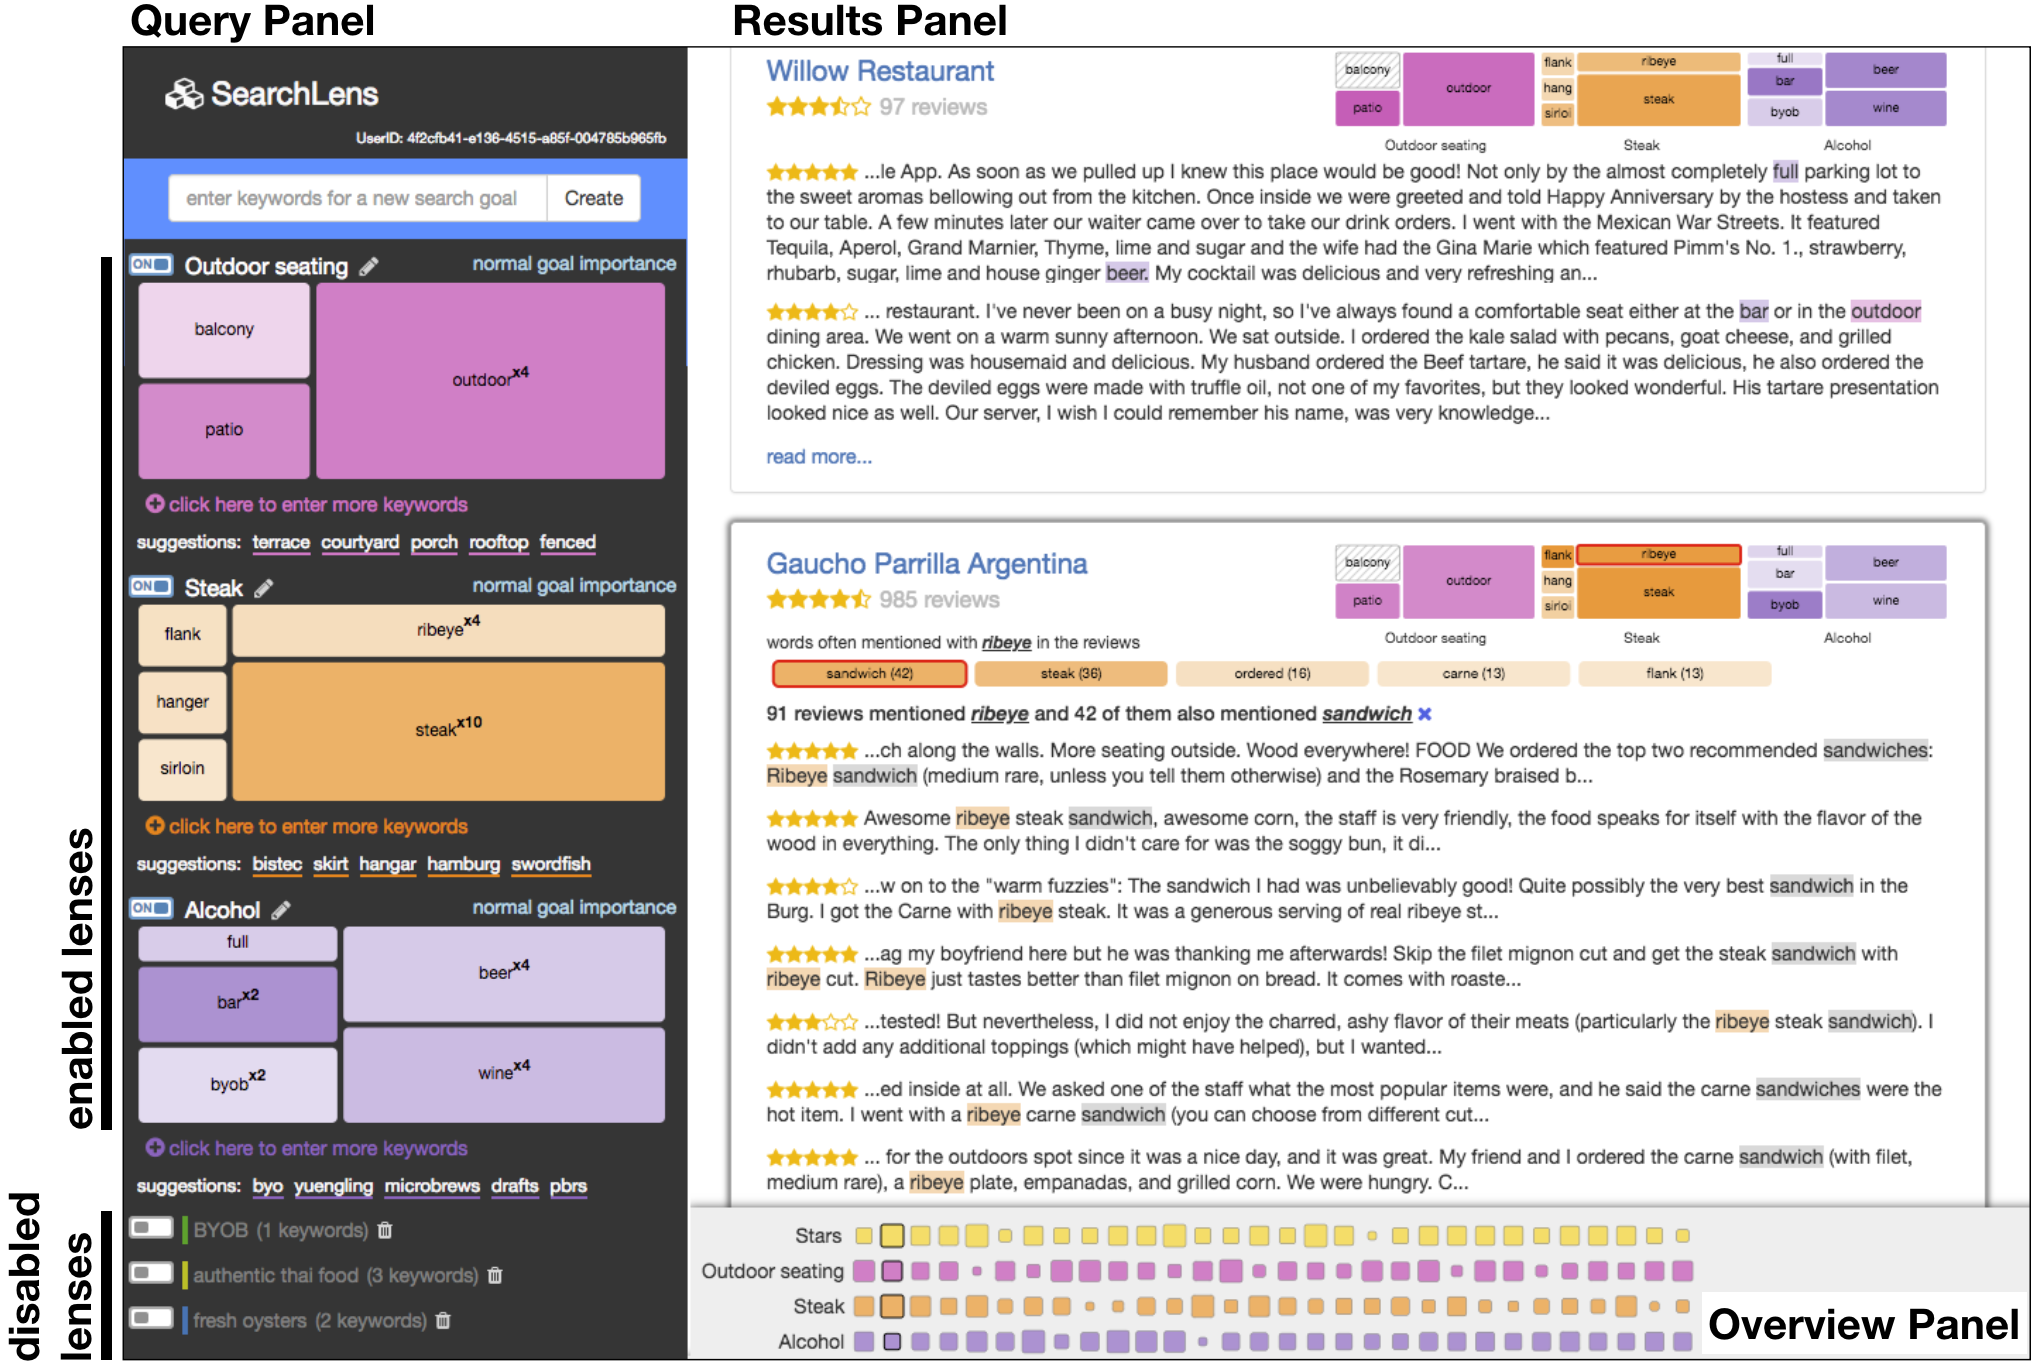
\includegraphics[width=1.0\textwidth]{Chapters/SearchLens/figures/main_annotated.png}
    \caption[An overview of the SearchLens system.]{An overview of the SearchLens system. The Query Panel on the left allows users to specify search topics, or Lenses, by specifying multiple keywords. The keywords for a given Lens are show in colored cells sized by importance (weight). Lenses can be freely disabled or enabled for different scenarios. The Results Panel on the right shows a ranked list of search results that best match the enabled Lenses from the searcher. The same visualization for specifying queries are then used for explaining how each result matches with user's interests and mental model, and also serve as an interactive navigation for filtering mentions of specific keywords. The Overview Panel at the bottom shows a collapsed version of the cells that allows for quick comparison between results.}
    \label{fig:sl_flow}
\end{figure}

\section{Introduction}

People often rely on reading online reviews and forum posts to make predictions about how well different options might match their personal interests and needs.  With the proliferation of online reviews, people now have instant access to millions of online reviews from people with varying perspectives and interests. It was estimated that in 2013 Amazon provided shoppers access to more than one million reviews for just their electronics section \cite{mcauley2013hidden}, and in 2016 Yelp provided around 250,000 reviews for over 6,000 restaurants for the city of Toronto alone \cite{yelpdata}. Having access to this rich repository of diverse perspectives based on the past experiences of others has the potential to empower consumers to understand their choices thoroughly and make better decisions for themselves without being overly influenced by marketing and branding \cite{de2015navigating}.

%However, the diversity of the reviews also often makes aggregated information, such as average review ratings, not enough for people to make decisions, and finding relevant reviews and reading through to understand the decision space can be challenging and time-consuming because people must both discover important factors that might be relevant to them (e.g., long lines, dishes or ingredients that signal the authenticity of food) as well as evaluate how various options address those factors. Furthermore, once they have finished searching the work they did in discovering factors and evaluating options does not persist, resulting in them having to start from scratch even for a very similar need. For example, a traveler who has spent a lot of time choosing between ramen restaurants in Los Angeles must start from scratch evaluating ramen restaurants in Toronto, despite having discovered several important factors (e.g., thickness and chewiness of noodle, whether the broth is simmered for a long time with pork bones) that will be similarly utilized in their decision making.

% I added this back for people who might say why not just look at the scores
Unfortunately, it is often difficult for users to be able to quickly and efficiently match their personal interests to the large amount of information available for each potential option. One problem is that simple star ratings are often not sufficient, and recent research has shown reviews often play an important role in users online purchase decisions \cite{mudambi2010research,gan2012helpfulness}. For example, restaurants might receive negative reviews for its simple decor and lack of good ambiance, but some searchers might value more the authenticity of the food or whether vegan options were available on the menu. Subsequently, finding, reading, and evaluating relevant reviews is time-consuming and challenging. Users have to manually parse through the reviews for each restaurant and match them to their personal interests (e.g., kid friendly, authentic Indian cuisine). They then have to track which restaurant meets which criteria, and if they discover and add any additional criteria, they must back-fill that information and re-evaluate previously seen restaurants. Furthermore, once a user has finished searching, the work performed discovering and evaluating factors is lost, resulting in having to start from scratch even if a similar need arises in the future. For example, a traveler who has spent a lot of time choosing between ramen restaurants in Los Angeles must start from scratch evaluating ramen restaurants in Toronto, despite having discovered several important factors (e.g., thickness and chewiness of noodle, whether the broth is simmered for a long time with pork bones) that will be similarly utilized in their decision making.

Getting users to specify these nuanced interests and preferences has been a long standing challenge. Several decades of research have explored ways of getting users to externalize their interests \cite{jansen2000real,belkin2001rutgers}, for example by: using prompt and text field designs that promote longer query terms \cite{franzen2000verbosity,belkin2003query}, asking for relevance feedback on the results provided \cite{salton1990improving,rui1998relevance,peltonen2017negative}, or explicitly asking users to build up sets of query terms of different topics \cite{hearst1996visualizing,hoeber2006comparative}. There are two primary challenges brought up by this work. First, users have trouble specifying their interests, which includes challenges with identifying query terms that were neither too general nor too specific; providing more than a few terms (even when longer queries were more likely to lead to useful results); and learning terms from the content, rather than knowing them all beforehand  \cite{belkin2003query,salton1990improving}. The other main issue found is that it is very difficult to get users to put in the work to externalize their interests, either as query terms or as explicit feedback, due to perceptions that the work will not be sufficiently paid off in the future or not understanding how their work will affect their results. 
%% This is unnecessary and very repetitive with the previous paragraph

To tackle this issue of capturing, leveraging and exposing user interests, we introduce SearchLense, where users construct externalized representations of their interests as ``Lenses''. Lenses are leveraged as an explanatory tool, providing users with a way to quickly parse, understand and make judgments based on the vast amount of review data instantaneously. Additionally, Lenses can be reused in different contexts and combined in different configurations. In the example above, imagine a system which could capture the factors that the traveler found important for ramen in Los Angeles and reuse them to quickly make a confident, personalized decision about ramen in Toronto. If traveling to Toronto with kids, a ``kids'' Lens might also be added with factors such as whether the restaurant typically has long lines and how many seats it has. These persistent Lenses could be useful in a variety of situations beyond reviews, ranging from academics keeping track of interesting research topics; travelers deciding which places to visit in an unfamiliar city; consumers deciding between products; lawyers doing case discovery; or voters tracking important issues.
We explore this problem in the context of restaurant reviews, conducting a controlled lab study with 29 participants to examine if our visual interface for explanation and exploration is effective in providing immediate benefits to elicit rich interest expressions from the users. Additionally, we performed a three day field deployment study with 5 participants to explore the benefits of Lenses when users were conducting their own tasks. Results suggest that our prototype system SearchLens was able to learn richer representations of its users' interests when compared to a baseline system by allowing users to fluidly capture, build, and refine Lenses to reflect their interests and needs, and that the user-generated interfaces can be reused over time and transfer across contexts.


%% See Comment
%To understand the prevalence of these issues, we conducted a pilot survey with 50 participants recruited from Amazon Mechanical Turk (age between 21 and 63, M=37.0, SD=11.7, 52\% male, and 48\% female, mostly from the US), focusing on their experiences when researching restaurants online. We chose restaurant search as our main topic due to its subjective nature and the availability of large repositories of reviews with diverse opinions and preferences. Most of our participants (95\%) self-reported that they use services that provide reviews and ratings to look for restaurant information online. At the same time, 60\% of the participants agreed that do not always choose restaurants based on their average ratings. Participants also agreed that when searching for restaurants online, they had encountered restaurants with bad average ratings but were mostly about things that they did not care about (62\%), and that it is time consuming to sift through reviews to find ones that were of interest to them (60\%). This suggests that searchers often spend a lot of time and effort to carefully examine the reviews and identify relevant aspects and keywords that reflect their personal preferences and repeat this process across different scenarios.



% MERGED INTO (2) -- ; and 3) users do not understand how their interactions will affect their content. 
% i feel like (2) and (3) is potentially saying how the interaction of querying is agent-based since the relationship between input and output is unclear and can be unexpected, and we are making it towards direct manipulation by adding transparency 

%Supporting personalized explanation of items in a search results is challenging first because the interests and goals of an individual are often not fully specified in the query, and then were often further compressed by computational representations that can be difficult for humans to understand \cite{chuang2012interpretation}. 
%Consider for example an user interested in authentic Indian food -- this may be true at a high level, but perhaps that person also has a preference towards Northern Indian cuisine, and has particular specific favorites, such as \textit{pani puri} or \textit{samosas}. Or perhaps users are trying to look for \textit{outdoor restaurants} in a \textit{easy-to-park neighborhood} that have \textit{space for kids} to run around but also serve \textit{hoppy beers} and \textit{rye whiskey}. If these nuanced interests and soft criteria, while often key factors in decision making, are  not specified in the query terms, search systems would have little understanding of their users to generate personalized explanation for each result, leaving users to rely on closely examining many reviews to identify ones that were relevant to their latent interests in order to comprehend options in the search results.



% Results suggest that our prototype system SearchLens can:

% \begin{itemize}
% \item allow users to fluidly capture, compose, and reuse Lenses to reflect their interests and needs for different contexts
% \item allow users to interpret, explore, and discover desired results using personalized interactive interfaces instead of sifting through reviews in arbitrary order
% \item encourage users to express and refine their Lenses using significantly more keywords when compared to a baseline condition that does not support personalized explanation and exploration interfaces
% \end{itemize}

%However, the sheer amount of online reviews are often well beyond individuals capacity to process, prohibiting them to benefit fully from the these rich repositories of diverse information.
%While review services typically provide users with average rating score and rating distribution for each option, they provide little personalized insights into how each option matches with the interests of a particular user.  Supporting personalized explanation of items in a search results is challenging first because the interests and goals of an individual are often not fully specified in the query, and then were often further compressed by computational representations that can be difficult for humans to understand \cite{chuang2012interpretation}. Consider for example an user interested in authentic Indian food -- this may be true at a high level, but perhaps that person also has a preference towards Northern Indian cuisine, and has particular specific favorites, such as \textit{pani puri} or \textit{samosas}. Or perhaps users are trying to look for \textit{outdoor restaurants} in a \textit{easy-to-park neighborhood} that have \textit{space for kids} to run around but also serve \textit{hoppy beers} and \textit{rye bourbon}. Past work have shown that even expert searchers typically do not use more than a few query terms to specify their information needs, even when longer queries tend to lead to better results or higher user satisfaction in exploratory search scenarios \cite{belkin2003query}. As a result, these nuance interests and soft criteria, while often key factors in decision making, are rarely specified in a single query. This leaves search systems with little understanding of their users to generate personalized explanation for each result, leaving users to rely on closely examining many reviews to identify ones that were relevant to their latent interests in order to comprehend options in the search results.

% To understand the prevalence of this issue, we conducted a pilot survey with 50 participants recruited from Amazon Mechanical Turk (age between 21 and 63, M=37.0, SD=11.7, 52\% male, and 48\% female, mostly from the US), focusing on their experiences when researching restaurants online. We chose restaurant search as our main topic due to its subjective natural and the availability of large repositories of reviews with diverse opinions and preferences. Most of our participants (95\%) self-reported that they use services that provide reviews and ratings to look for restaurant information online. At the same time, 60\% of the participants agreed that restaurants they like do not always have high average ratings. Participants also agreed that when searching for restaurants online, they had encountered restaurants with bad average ratings but were mostly about things that they did not care about (62\%), and that it is time consuming to sift through reviews to find ones that were of interest to them (60\%). This suggests that even though modern search engines can return a list of options and reviews in split seconds, searchers often still need to spend a lot of time and effort carefully examining each result to find parts that are relevant to them before they can start comparing their options and make decisions.
% For example, looking for reviews that describe a particular drink, or whether the environment was kid friendly.

%An alternative approach is to annotation each item in the dataset of with different criteria, subtopics, and attributes, whether using expert labelers or computational techniques \cite{}, and present these metadata to the users using faceted search interfaces \cite{hearst2006design}.
%While expert annotation have found to be useful for providing an overview of a large number of choices (e.g., products, restaurants), allowing users filter and navigate to different options based on objective criteria (e.g., price range, location), it is unlikely for it to scale and support the above mentioned subjective interests and needs (e.g., good date night restaurants). For this, prior work has also explore ways to extract aspects and subjective judgments from the reviews using computational approaches. However, 

%In summary, we suggest to design exploratory search interfaces that can provide personalized explanations and exploration interfaces for each search result, and encourage users to express their rich latent interests in order to enable these benefits. In addition, many preferences (such as \textit{hoppy beers} and \textit{rye bourbon}) might be relevant for multiple contexts, such as on a date night or going out for drinks with friends in different neighborhoods, and allowing users to structure and persist keywords that describe their different interests can further reduce future efforts. This also has the benefit of encouraging users to refine their query terms to be used again in the future, since some of the terms that might seem to be good at first might in fact not be very discriminatory (e.g., \textit{great}, \textit{delicious}) versus less obvious terms that act as more ``honest signals'' (e.g., the use of the word \textit{bone broth} for ramen broth that is simmered for days).  

% In this paper we explore a novel interface that allows users to specify and maintain their multifarious and idiosyncratic search goals with structured queries that we call Lenses, and gradually construct an personalized interactive search interface based on their own interests and past activities. With the rich interest profiles specified by the users, the system can provide personalized visual explanation of items in a search results beyond average ]rating scores. The visual explanations also serve as personalized interfaces that allow users to surface reviews that matches their different latent interests for deeper  xploration. The instantiation of this approach is a prototype system called SearchLens, which allows users to progressively and persistently build up a repository of ``Lenses'' that can be used to reflect their latent topics of interests and mental model. Users construct Lenses by specifying keywords and weights, and the system visualizes the importance and frequency of each keyword in the results for comparison. Besides specifying keywords from prior knowledge, SearchLens also provides a mechanism for users to discover and collect keywords as they look at the search results. In addition, the system provides suggested keywords for each Lens using a semantic word vector model. The Lenses that users create persist across sessions, allowing users to freely enable and disable different sets of Lenses for different occasions. For example, enabling their Lenses for ``kids friendly'', ``easy parking'', and ``home cooking'' to explore restaurant options for a big family dinner, and enabling their Lenses for ``cozy and intimate'', ``easy parking'', and ``good wine selection'' to explore restaurant options for date night. These Lenses in turn allow the system to present each result based on the current interests of the users, and allow them to explore each of the results by revealing mentions of different query terms. We conducted a lab study with 29 participants, and a field study with 5 participants conducting their own tasks over 3 days. 
%In addition, we also show that standard information retrieval systems (i.e., document search engines) can be easily adapted to support these interactions with high efficiency and scale. 


% In this paper we explore a novel interface that allows users to specify and maintain their multifarious and idiosyncratic search goals with structured queries that we call Lenses, and gradually construct an interactive search interface based on their own interests and past activities. The instantiation of this approach is a prototype system called SearchLens, which allows users to progressively and persistently build up a repository of ``Lenses'' that can be used to reflect their topics of interests and mental model. Users construct Lenses by specifying keywords and weights, and the system visualizes the importance and frequency of each keyword in the results for comparison. Besides specifying keywords from prior knowledge, SearchLens also provides a mechanism for users to discover and collect keywords as they look at the search results. In addition, the system provides suggested keywords for each Lens using a semantic word vector model. The Lenses that users create persist across sessions, allowing users to freely enable and disable different sets of Lenses for different occasions. For example, enabling their Lenses for ``kids friendly'', ``easy parking'', and ``home cooking'' to explore restaurant options for a big family dinner, and enabling their Lenses for ``cozy and intimate'', ``easy parking'', and ``good wine selection'' to explore restaurant options for date night. These Lenses in turn allow the system to present each result based on the current interests of the users, and allow them to explore each of the results by revealing mentions of different query terms. We conducted a lab study with 29 participants, and a field study with 5 participants conducting their own tasks over 3 days. Results show that our prototype system SearchLens a) allows users to fluidly capture, build, and refine Lenses to reflect their interests and needs, b) allows users to interpret, explore, and discover desired results using the interactive interfaces, and c) that the user-generated interfaces can be reused over time and transfer across contexts. In addition, we also show that standard information retrieval systems (i.e., document search engines) can be easily adapted to support these interactions with high efficiency and scale. 


\section{Related Work}

%In this work, we propose to support users to fluidly express and curate their different interests and criteria using ``Lenses'', and allow them to freely compose, and reuse their previously specified interests across different contexts. One key challenge is to provide immediate and sufficient benefits to the users in order to elicit their rich interests. For this, we propose to not only use users' Lenses as a way to retrieve rel event items, but also to provide visual explanations for each item and enable deeper exploration. 

Past research has proposed a variety of approaches to collecting, modeling and leveraging users' interests and intents through both interface design and computation. Our work builds on this diverse of literature by allowing the system to learn the personal interests of the users through interaction to retrieve relevant data, and present data based on its understanding of the different users. This allows us to elicit structures that can be reused across different contexts and tasks and are more nuanced and personalized to each users when compared to traditional search structures such as search results clustering or pre-compiled facets.

% Unlike simple and objective information seeking scenarios, such as finding the address of a restaurant or checking the weather, in review search scenarios, different searchers typically have varying interests and criteria, but at the same time, the reviews themselves are often also multifarious and subjective in nature and therefore do not always match the interests of every searcher \cite{mar2006exp,de2015navigating,mudambi2010research,gan2012helpfulness}. As a results, a searcher might needs to sift through many reviews to find ones that are relevant, or come up with a set of discriminative keywords for each of his or her different interests or criteria.

% Despite their ubiquity, operations for searching with multiple topics of interest as described above are poorly supported by modern approaches. Search engines have optimized for providing information as quickly as possible \cite{teevan2013slow}, such as knowledge cards in which an answer is surfaced directly on a search results page or visual carousels of possible options that a user can quickly click through \cite{yi2009discovering,bota2016playing}. These approaches excel at finding answers to objective, factual questions, but notably fail to address activities involved in complex, personalized search tasks, such as specifying multiple goals and criteria, explaining search results based on personal interests, and allowing for deeper exploration of different options for comparison \cite{marchionini2006exploratory,white2006supporting,white2009exploratory}.

% As a result, the search result list can become increasingly difficult to interpret as the user adds more keywords to their query, raising questions like how different keywords influenced the ranking, and whether each result matches with their different topics of interests. Further, in order to explore deeper to get a better understanding of their options, users would need to leave the search result list page and visit each result independently and manually extract parts that are relevant to their goals, often with the in-page keyword matching provided by the browser. 

\subsection{Eliciting and Modeling Interests and Intents}

A significant topic of research has been interfaces that can collect, explicitly or implicitly, the personal goals and interests of users as they search for information and modify their viewing of content correspondingly. While there is extensive literature on doing so in the context of personalized search and re-ranking of search results (e.g., \cite{speretta2005personalized,shen2005implicit,burges2005learning,cao2007learning}), we focus here on work that enables more interactivity and transparency of users' interests to support more complex searching.  One such thread lies in the collection of users' interests through keywords or interest vectors into an agent or user interest or intent model. This includes seminal work such as WebMate \cite{chen1998webmate}, which built up an agent composed of sets of TF-IDF \cite{wu2008interpreting} vectors to represent the user's different interests. Similar to WebMate, we aim to build collections of terms that represent the user's interests, but focus on explicit user selection of those sets, and making them explainable and composable. Interestingly, WebMate's ``Trigger Pair Model'' which looked at co-occurrence of words within a sliding window across a set of documents can be seen as a precursor to the word vector model that we use for keyword suggestions.  More recent work in this vein includes user modeling of concepts, such as AdaptiveVIBE \cite{ahn2009adaptive} and Intent Radar \cite{peltonen2017negative}, which include two dimensional visualizations of documents and their relation to the user's inferred interests. Our work builds upon these but aims at increasing the richness of the structure, nuance, and specificity of the user's expression of interests. Specifically, our Lenses, composed of multiple keywords that can capture multiple levels of specificity, can be themselves composed into more complex expressions and reused across different contexts and tasks. We also focus on supporting users in the discovery process of building good terms that are discriminatory and explanatory.


%\subsection{Exploratory Search Interfaces}

%A major thread of work that we draw on includes novel personalized search interfaces such as semantic web interfaces \cite{wilson2006mspace}, or computational approaches such as automatic or interactive result clustering \cite{cutting2017scatter}. Several exploratory search interfaces have been developed in order to help searchers orient themselves in the information space, review and explore the different subtopics, and keep track of their overall progress \cite{hearst2009search,marchionini2000agileviews,patterson2001predicting,tretter2013searchpanel,morris2008searchbar}. Two closely related studies include Topic-Relevance Map and Exploration Wall, which explored ways to provide overviews of search results of academic papers using document keywords and entities and easily choose keywords to build up subsequent queries \cite{peltonen2017topic,klouche2015designing}. In SearchLens, instead of proposing subsequent queries to the users, we instead propose potentially useful keywords to be incorporated into users' existing Lenses, and provides visual explanations for each item that are capable of scaling to many query terms. This allows users to query with many query terms instead of switching between different more focused query, while still being able to easily comprehend how each result matches with their different latent interests.

% https://www.researchgate.net/publication/221300933_An_Aspectual_Interface_for_Supporting_Complex_Search_Tasks



\subsection{Concept Discovery and Evolution}

Research in interactive machine learning has also explored techniques to support data annotators or searchers in discovering and externalizing useful concepts when working in unfamiliar domains. 
%Another line of research in interactive machine learning explored using visualization and interaction techniques to better support discovering, externalizing, and refining useful concepts while exploring and labeling data in unfamiliar domains.
For example, Alloy used a \emph{sample-and-search} technique to categorize textual datasets with novice crowdworkers where they first explore the space of information through sampling items in the dataset to discover useful categories, then externalize each category using a set of query terms and search for other relevant items \cite{alloy}.
Past work has further suggested that the working concepts of an annotator may change over time as new items were examined \cite{kulesza2014structured}. Different techniques that can better support this concept evolution process were proposed, such as structured labeling \cite{kulesza2014structured}, crowd collaboration \cite{Chang:2017:Revolt}, and interactive visualization \cite{chen2018anchorviz}.  These point to the importance of providing mechanisms that allow users to not only discover and define concepts based on data, but also to easily evolve their concept representations during the process of exploring an unfamiliar domain.
In a study more closely related to our work, CueFlik allowed image searchers to define conceptual filters (e.g., listing only \emph{action shots} when searching for \emph{baseball} images) by labeling items in a search result list as positive or negative training examples \cite{fogarty2008cueflik}. Previously defined filters are persisted and can be applied to future searches (e.g., applying the same \emph{action shots} filter when searching for \emph{football} images), but evolving existing conceptual filters would require recreating filters from scratch or re-labeling items in existing filters.
Our work builds this past work to allow exploratory searchers in unfamiliar domains to discover concepts of interests from data and externalize these concepts in the form of ``Lenses'' that can be continually refined. Finally, the Lenses are persisted across different search sessions similar to \cite{fogarty2008cueflik}, and can be modified and composed for different scenarios and goals.
%(e.g., \emph{ramen shops} with \emph{outdoor seating} and serves \emph{unfiltered sakes}).
%(e.g., seeing multiple reviews mentioning \emph{thick bone broth} when searching for ramen restaurants).



% Alloy
    % sample-and-search to help turkers define useful concepts in known-known thru picking out query terms
% ConceptEvo, Revolt
    % concept may drift even for simple concepts (i.e., cats unlike "has a good bar")
    % provide techniques to help discover concepts through crowd collaboration and structured labeling
% AnchorViz - use viz to 
    % find items with new features that helps classifier
    % an interactive visualization that facilitates error discovery through semantic data exploration.
    % discover more prediction errors
% CueFlik
    % in image search task, users can help machine better identify their intent through defining concepts by providing positive and negative feedbacks


\section{System Design}

%The key motivating concept behind SearchLens was providing users with a way to externalize the complex mental models of their interests in a way that could be useful for themselves in understanding their information space immediately and in the future.  We aimed to make the interface simple and transparent but also powerful enough to express hierarchy and support multiple concepts and levels of specificity.  To do this we introduced the idea of ``Lenses'': reusable collections of weighted keywords that contain ``honest signals'' of a user's interests that can be composed in different configurations to match a user's current needs. The Lenses that are enabled in a particular configuration drive various visualization and explanation elements to help the user understand how the information space meets their needs, and also whether they need to fix or reformulate their Lenses. 

The key motivating concept behind SearchLens was providing users with a way to externalize their complex interest profiles in a way that could be useful for ranking, explanation, and transference to different contexts. We aimed to make the interface simple and transparent but also powerful enough to express higher level, abstract concepts and differing levels of specificity.
To do this, we introduce the idea of ``Lenses'': reusable collections of weighted keywords that contain ``honest signals'' of a user's interests that can be composed in different configurations to match a user's current needs. The Lenses that are enabled in a particular configuration drive various visualization and explanation elements to help the user understand how the information space meets their needs, and also whether they need to fix or reformulate their Lenses. 

A key challenge here is incentivizing users to create rich Lenses by providing sufficient and immediate benefits. For this, SearchLens provides visual explanation of items in the search results based on users' Lenses, which also serves as an interface for deeper exploration. When a new Lens is created or enabled, its visual representation appears on the interface for each item, allowing users to understand how well each item matches with the Lens, and how frequently each keyword is mentioned in its reviews. To further explore each item, users can click on keywords in each Lens to see relevant reviews.

A typical use case is as follows. A user just moved to Pittsburgh and wants to go out to eat ramen. She starts by pulling up a restaurant she knows she likes from Toronto and goes through some of the reviews, noticing that the reviews of her favorite tonkatsu ramen mention interesting signals such as ``bone'' and ``umami'' and adds them to her ramen Lens along with other useful words such as ``tonkatsu'', ``ramen'', ``bowl'', etc. After checking to see that her Lens is bringing up other restaurants that serve ramen she likes in Toronto and adding a few of their terms to her Lens, she switches to Pittsburgh and looks for how her Lens is being used.  She also activates her drinks Lens, which she's built up over time to incorporate her particular interests in unfiltered sakes as well as hoppy beers. Using the Lenses, she quickly see which ramen restaurants in the results list serve unfiltered sakes and/or hoppy beers. To further explore her different options, she can click on each keyword in her Lenses to filter relevant reviews. For example, ``tonkatsu'' might be often mentioned with ``spicy'' in one restaurant, and ``creamy'' in another, allowing her to further differentiate her options based on aspects that she cares about.

The following subsections describe the designs of the SearchLens system. We will first present our concept of ``Lenses,'' and how users can use SearchLens to fluidly express and refine their different nuanced interests, and freely compose their Lenses for different contexts. We will also describe how search Lenses can provide immediate benefits once specified, providing users visual explanation of each item in the search results, and also an interface for deeper exploration.

%As an overview of the system, Figure~\ref{fig:sl_flow} shows an example use case of SearchLens, which addresses the issues in the following way:

%\begin{itemize}
    
%    \item \textbf{Query specification} The query panel on the left allowed users to specify structured queries, or Lenses, that reflect their different search goals. A treemap \cite{shneiderman2001ordered} is presented for each search lens that illustrate the set of user-specified keywords (cells) and corresponding importance (sizes of each cell). The overall frequencies of query term in the results (shading of each cell) is also presented to show how the results reflect the expectations of the users. (Figure~\ref{fig:sl_flow}, left)
    
%    \item \textbf{User-generated interface} Lenses are persisted between visits to the system. As users perform more searches, they gradually build up a repository of their personal Lenses that reflects their different interests and goals. The users can freely enabled or disabled different sets of Lenses for different or recurring scenarios. (Figure~\ref{fig:sl_flow}, left)
    
%    \item \textbf{Explanation} The user-specified Lenses are also used for providing an overview for each search result. The same treemap visualization shows the frequencies of each query terms within each search result to help users interpret each result efficiently using the familiar visualization that they created when specifying their search goals. A collapsed version of the treemaps are shown in the bottom panel for overview and quick comparison. (Figure~\ref{fig:sl_flow}, right and bottom)
    
%    \item \textbf{Exploration} The user-specified Lenses are also used for navigation for deeper exploration. User can click on their query terms to see their mentions for each search result in real-time. SearchLens also show frequently co-occurring terms in cases where a lot of mentions exist.  (Figure~\ref{fig:sl_flow}, right. Figure~\ref{fig:sl_compare})

%\end{itemize}

%In the following subsections, we describe in detail the domain and data source we used, the design and implementation of each component, and a scalable backend ranking method that powers the interactions.

%\subsection{Domain and Data Source}

To test our prototype system in a realistic and manageable setting, we focused on the domain of restaurant reviews where personalization and searching with multiple goals is especially important. We used a subset of the dataset from the Yelp challenge \cite{yelpdata} that included local business in 11 metropolitan areas.\footnote{Pittsburgh, Charlotte, Phoenix, Las Vegas, Toronto, Montréal, Mesa, Mississauga, Cleveland, Scottsdale, and Edinburgh.} Restaurants and reviews were selected by string matching on the \emph{city} field of each restaurant available as metadata in the Yelp challenge dataset, resulting a subset of 48,485 restaurants and 2,577,298 reviews. This allows us to explore how user-specified Lenses can be composed and reused for different scenarios, as well as for the same scenario across different cities. In addition, we also use the same data to train a Word2Vec model \cite{mikolov2013efficient} for generating Lens-specific query term suggestions.


\subsection{Capturing User Interests with Lenses}

Our goal was to develop a way to elicit users' interests which is both highly expressive and immediately beneficial. To explore the natural discovery and collection of users' interests we conducted a preliminary study in which we asked people to read reviews of their favorite restaurants on Yelp and see if they could identify terms that were good indications of their interests. We discovered that people found it intuitive to identify many different terms that matched their interests. Many of these terms were not simply general descriptors (e.g., ``good'', ``tasty'') but instead terms they considered indicative of matching their personal interests (e.g., an authentic ramen restaurant would include terms talking about the thickness of the noodles; a popular restaurant might be less favored if it also had very long lines). Terms also fell into different classes of factors users were interested in (e.g., service vs. food quality vs. parking). Users seemed to focus on finding reviews that mentioned these terms and use them in their decision making.

Based on these initial findings we developed a system for users to easily collect terms from reviews into ``Lenses'' and to use those terms to identify and summarize reviews that mentioned those terms. Similar to \cite{hearst1996visualizing}, we enable users to search with multiple Lenses at the same time. However, our Lenses differ from traditional search queries or faceted metadata in several important ways. 

First, our system encourages the iterative development of Lenses as the user explores. A common activity in online exploratory search involves discovering new and interesting aspects from data. SearchLens aims to make it easy for users to add new Lenses and improve existing ones throughout their searching process. Users can create a new Lens by specifying a set of keywords using the text field in the Query Panel on the left (Figure~\ref{fig:sl_flow}). As users browse the results on the right, they might find some keywords in their Lenses were too general to be useful (e.g., ``tasty broth''), and find discover more indicative keywords either from prior knowledge or from the reviews (e.g., ``rich and thick broth''). In this case, users can refine their Lenses by adding new keywords using three different interactions, each for a different scenario. First, users can click on the plus icon under each Lenses to enter new keywords in a Lens specific text field. Second, as users discover more indicative keywords or new topics of interests from the reviews, they can highlight the keywords and use a context menu to add them to an existing Lens. In addition, a list of keyword suggestions are also listed under each Lens based on current keywords (Figure~\ref{fig:sl_suggestion}). Users can hover over each suggestion to see example mentions, and click on the keyword include it. This allows users to assess the usefulness of the suggestions, such as to avoid ambiguous terms. The Lens-specific suggestions were computed based a word semantic model described in the below subsection. To remove a keyword, users can click on its cell and select remove keyword in the context menu.

%, and refining query with more indicative terms. However, traditional search interfaces typically only allow users to specify bag-of-word queries, providing no structures for users to express their different search goals and criteria. Further, one's many interests are likely to be useful across different contexts, but the ephemeral nature of traditional search interfaces typically does not support reusing previously specified interests, and discourages users to spend much effort in fully expressing their multifarious interests and refining their query terms.

%SearchLens support these needs by allowing users to specify sets of keywords and weights that describe different topics of interests we call Lenses, and supports searching with multiple Lenses at the same time (similar to \cite{hearst1996visualizing}). 

Once constructed, Lenses can then be used to visually inspect and adjust their ``projections'' onto the data. Lenses are represented visually as boxes subdivided into cells, one for each term the user added. Initially, all keywords in the same Lens have equal importance (as reflected by being the same size), but users can click on each cell to select different importance in a context menu (x1, x2, x4, x10, exclude) to better reflect their personal preferences. The size of the cells will adjust accordingly to reflect the importance of each keyword (excluded keywords are represented using fixed size cells with a unique pattern fill). The shade of each cell shows the overall frequency of each keyword in the top 30 search results (Figure~\ref{fig:sl_flow}, Query Panel). This allows the user to get a sense of how items in the corpus reflect their mental representation of each topic. For example, a large cell with very light shade represents a concept that the users deemed as an important feature of the topic, but was rarely found in the results. Surfacing this information ensures user are aware of how useful each of their keywords are, and can refine their Lenses to include more indicative keywords.



%SearchLens also allows users to specify the importance of each query term using the treemap visualization to better reflect the users' mental representation of each topic. The size of each cell illustrates the importance of each keyword as specified by the users. To adjust the importance of a keyword, a user can click on it and select a different level of importance in a context menu, and the treemap will resize the cells accordingly. The importance levels (x1, x2, x4, and x10) directly correspond to the keyword and lens weight in the backend ranking function, which will be described in detail in a later subsection. 

As Lenses and terms are collected a user can over time build up a repository that reflects her personal interests. Each Lens can be disabled and re-enabled and are persisted across different visits to the SearchLens interface, with disabled Lenses are listed at the bottom of the Query Panel (Figure~\ref{fig:sl_flow}). Various combinations of Lenses can be activated depending on the goal and context. For example, for a date night a user might enable their personalized Lenses for ``cozy and intimate'', and ``vegan'', or for a weekday lunch activate their Lenses for ``fast casual'', ``vegan'', and ``easy parking''. Although our main thrust in this chapter is exploring the viability of this approach, further work will likely be needed to understand as Lenses accumulate how to scale them. For example, in the current prototype all disabled Lenses are shown, but future systems could further contextualize Lenses by inferring the task context (e.g., what type of item someone is searching for). %Alternatively, users can use a single lens to create curated list of recurring criteria. For example, creating a lens for top ramen shops to try with keywords such as \emph{ramen}, \emph{broth}, \emph{savory}, \emph{authentic}, and \emph{tonkotsu}.
%Although in this case the Lens would become less composable as it includes multiple topics. In our study, we observed different behavior from different participants and under different conditions. We will present detailed results in later sections.


%\begin{figure}[]
%    \centering
%    \includegraphics[width=1\columnwidth]{figures/explain.png}
%    \caption{}
%    \label{fig:explain}
%\end{figure}

\subsubsection{Keyword Suggestions}

\begin{figure}
    \centering
    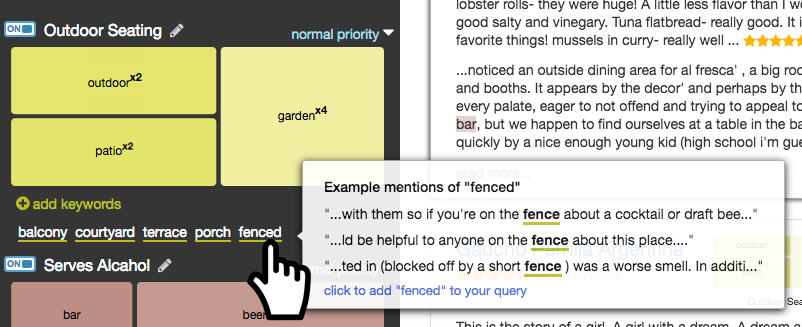
\includegraphics[width=0.6\columnwidth]{Chapters/SearchLens/figures/suggestions.png}
    \caption[SearchLens provides keywords suggestions based on currently Lenses.]{SearchLens provides keywords suggestions based on currently Lenses. Hovering shows a preview panel with mentions of the suggested keyword, allowing users to better understand the effect of adding the suggested keyword. In this case, SearchLens suggested balcony, terrace, fenced, and other keywords for the ``Outdoor Seating'' Lens. However, further inspection showed that fenced may not be a indicative keyword for the purpose of this Lens.}
    \label{fig:sl_suggestion}
\end{figure}


While creating a new Lens, listing all keywords from prior knowledge can be mentally taxing and have poor recall. To further reduce the required effort for building expressive Lenses, SearchLens generates Lens-specific keyword suggestions. As an example, when a user created an ``Outdoor Seating'' Lens with only three keywords (``outdoor'', ``patio'', and ``garden''), SearchLens automatically suggested relevant keywords including ``balcony'', ``courtyard'', and ``terrace'' (Figure~\ref{fig:sl_suggestion}). To do so, we trained a Word2Vec model \cite{mikolov2013efficient} with 300 dimensions using the entire Yelp dataset of 2,577,298 reviews. The trained word model can project words onto a semantically meaningful vector space, which in turn allows for measuring semantic similarity between words. Alternatively, it can also be used to find a set of words that are semantically similar to a given term by searching in the vector space of nearby words. To generate Lens-specific keyword suggestions, we first project all its keywords in a Lens onto the vector space and calculate the average vector to obtain a list of similar terms around the average vector. To further increase the chance of presenting useful and discriminatory search terms, we only used terms that appeared more than 50 times in the corpus, were mentioned in reviews of more than three restaurants, and were mentioned in less than 40\% of all restaurants.


\subsection{Interest-driven Explanation}

Persistent, decoupled user interest models would be beneficial to users the long run by providing separate reusable and recomposable interests across multiple search sessions. However, without immediate and perceivable benefits, users typically are not willing to spent extra effort expressing their separate interests for future tasks. For this, SearchLens uses each user's Lenses to provide visual explanation of each item in the search results. This is based on our approach of allowing users to express their multiple topics of interest separately, which enables SearchLens to distinguish between keywords of different topics and opens the possibility of visualizing each result according to users' interests in easy-to-interpret ways. Explanation is especially important for supporting searching with multiple interests, as it can be difficult for the users to understand which interests and keywords were associated with each result. Consider traditional search interfaces that only offer a short snippet for each result as explanation. These short summaries provide little support for personalized interpretation beyond a few highlighted query terms and their context. Even if users listed keywords of many different topics at once, the linear result list also provides little information about each result beyond their overall relevance ranking.

One obvious approach to explaining items in the search results is to surface mentions and statistical information, such as mention frequencies, at the topic level. For example, \cite{hoeber2006comparative} visualized the overall frequency of different search terms in different topics for each search result, and \cite{hearst1996visualizing} visualized the mention locations of different topics within each document. Visualizing at the topic level allowed these systems to provide mechanisms for specifying many topics and keywords, while at the same time visualized deeper information about each result in a way that matches the mental model of the searchers. However, visualizing at the topic level can be prohibitive for keyword-level operations, such as query reformulation and assigning importance levels to different keywords based on their frequencies.

\begin{figure}
    \centering
    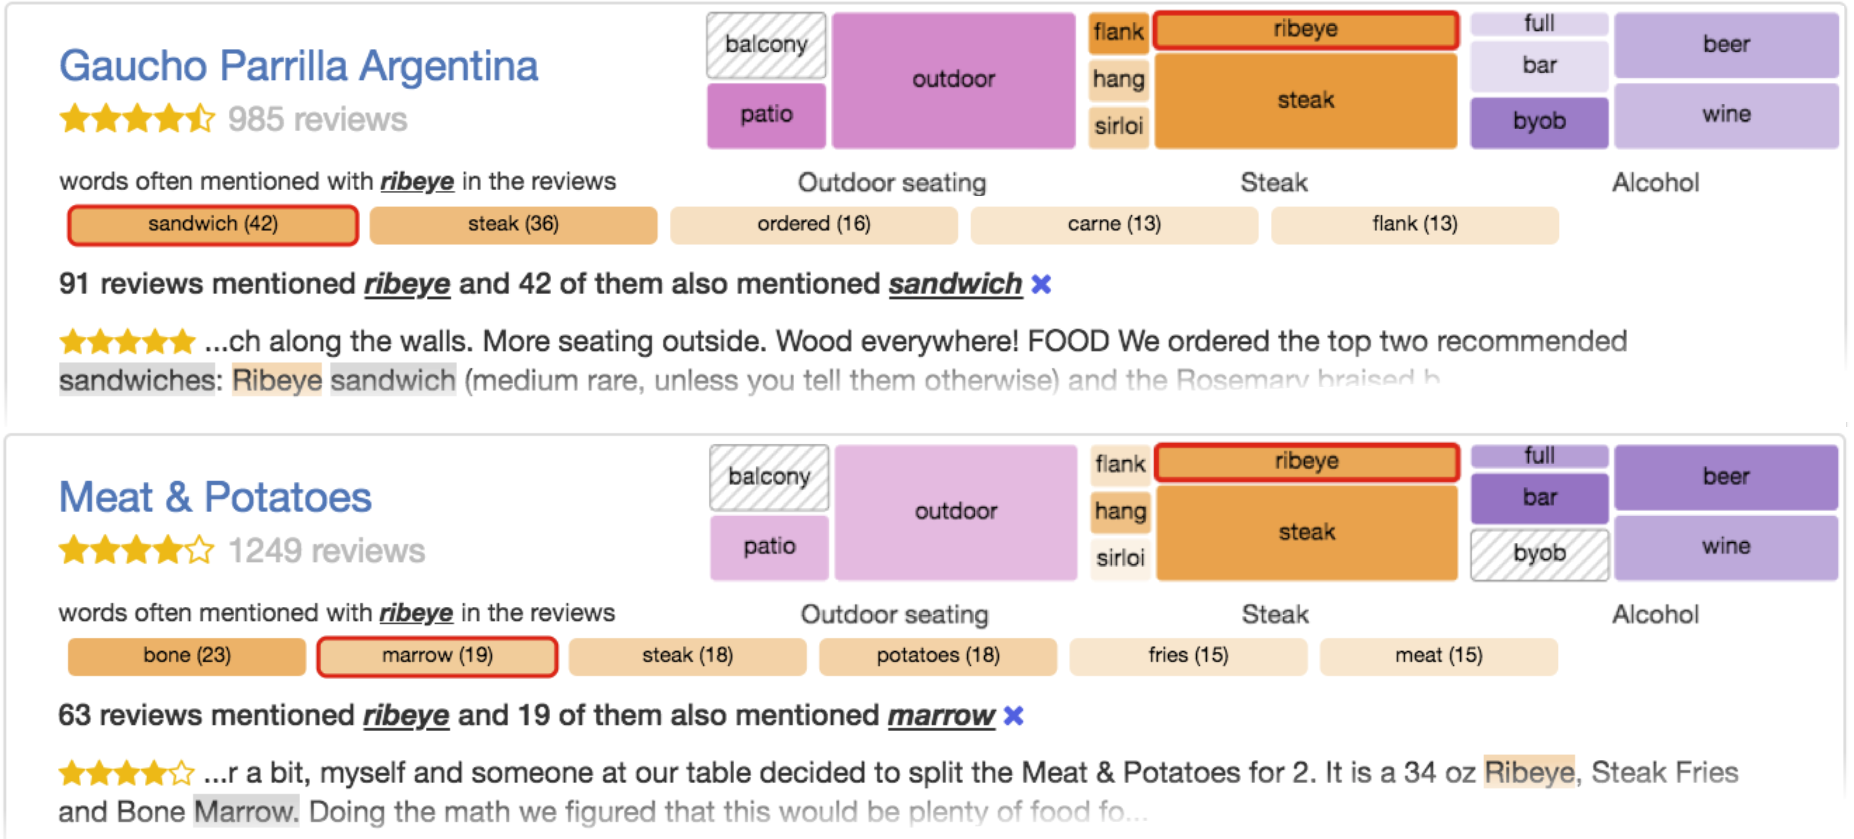
\includegraphics[width=0.8\columnwidth]{Chapters/SearchLens/figures/compare2.png}
    \caption[The visual explanation and exploration feature of SearchLens.]{The visual explanation and exploration feature allows comparison of results at different levels of granularity using a familiar interface used for specifying queries - at the levels of Lenses, keywords, co-occurring terms, and mentions, allowing users to query with multiple Lenses at the same time, while still being able to comprehend how each result matches their different Lenses.}
    \label{fig:sl_compare}
\end{figure}


% TODO messy -- should be fixed @nhahn thanks! @joseph
SearchLens supports rich explanation at the topic and keyword level through its user-specified Lenses. Explanation occurs by showing the each Lens visualization from the Query Panel (Figure~\ref{fig:sl_flow}) on each result and adjusting the term shading to correspond to the frequency of the term within that search result (Figure~\ref{fig:sl_compare}). By using identical colors and layouts of each Lenses, and showing result-specific keyword frequencies, users can quickly interpret how each result matches with their different interests at both the topic and at the keyword level using a familiar visualization. As an example, Figure~\ref{fig:sl_compare} shows how a user might examine two restaurants in a search result list using her Lenses for ``Steak'', ``Alcahol'', and ``Outdoor Seating''. At the topic level, both restaurants matched well with her Steak Lens rendered in dark shades that incorporated her stronger preference for ``ribeye'' steak, and also also her other interests such as ``flank'' steaks. She can also see that the first restaurant matched her Outdoor Seating Lens better than the second one. Looking at the same Alcohol Lens at the keyword level, she can easily see that the two restaurants matched differently with her ``Alcahol'' Lens where the first one has many mentions of ``byob'' in the reviews and the second one with many mentions of ``beer'' and ``bar'' instead.

%the she can easily infer that both restaurants have no reviews that mentioned her ``whisky'' keyword, and that the second restaurant also has very few mentions of ``cocktail'' as it is rendered in a light shade.

Finally, to provide a more compact, higher-level, topic-centric overview of all restaurants in the search results, SearchLens collapses the colored cells for each Lens into a single cell similar to \cite{hoeber2006comparative}. The size of each cell to shows the overall frequencies of keywords in different Lenses for each result (Figure~\ref{fig:sl_flow}). This allows users to get a quick overview of restaurants in the search results, and compare different options at the topic level using the Overview Panel at the bottom.


\subsection{Supporting Deeper Exploration of Items}
 

In addition to acting as a visual explanation for each result, the cells in the visualization also act as a navigation tool for deep exploration at the keyword level. Users can explore mentions of different keywords by clicking on its corresponding cell and the summary will update in real-time to show a list of its mentions. In addition, the Lens also shows the top co-occurring words that were frequently mentioned near the selected keyword as overview and deeper navigation, a strategy found useful in exploratory scenarios by prior work \cite{di2018study,di2016rank,peltonen2017topic}. As an example, Figure~\ref{fig:sl_compare} shows the how the Lenses allow users to explore and compare options at different levels of granularity. At the highest level, users can use the shading of different cells to see that the \emph{Outdoor Seating} Lens has more mentions in the first restaurant (Figure~\ref{fig:sl_compare}). Searchers can use the shading of individual cells to compare options at the keyword level. For example, the term ``BYOB'' was frequently mentioned in reviews for the first restaurant, but did not show up in reviews for the second restaurant. Finally, clicking on the individual cells allows users to explore mentions of its corresponding keywords and words that were frequently mentioned together. For example, when exploring mention of the work ``ribeye'' for both restaurants, SearchLens shows that there were many mentions of ``sandwich'' near the word ``ribeye'' for the first restaurant, and many mentions of ``bone marrow'' near ``ribeye'' for the second restaurant (Figure~\ref{fig:sl_compare}).



\subsection{Indexing and Ranking}

Traditionally, faceted search systems typically combine factors from multiple facets for ranking using disjunctions (factors within facets, such as brands selected by the user on a shopping website) and conjuctions (factors between facets, such as brands and price ranges). In an early iteration of SearchLens, we tested using the Boolean OR operator between keywords within the same Lens, treating keywords within the same Lens as synonyms while ranking. However, users reported this approach lead them to restaurants that poorly reflected their Lenses, as some restaurants may have many mentions of few keywords in a Lens, but very few mentions of other keywords. Fundamentally, unlike faceted search systems, different keywords in the Lenses typically describe a criteria as a whole. For example, an authentic ramen Lens might contained keywords describing creamy bone broth and freshly made noodles. In this case, the different keywords combined represented what the user considered good ramen restaurants, instead of as alternate options in a facet (such as a set of preferred brands). In a later iteration, we switched to Okapi BM25 for ranking that used inverse document frequencies to weight keywords instead of eliciting importance rating from the users. However, users reported unable to construct Lenses that reflect their priorities and unable to construct expressive Lenses that lead to useful results. This lead to the current iteration where we used a modified version of the standard Okapi BM25 ranking function to combine keywords across Lenses \cite{robertson2009probabilistic}, which by default considers both term frequency and document frequency to rank documents similar to TF-IDF ranking function, but also adjust for the length of each documents.

We modify the Okapi BM25 ranking function to account for the importance levels specified by users in the following ways. By default, Okapi BM25 uses the inverse document frequencies to weight each keywords, with the motivation that words appearing in many documents tend to be less important. Since in SearchLens users can specify keyword importance using the interactive visual explanation, we instead weight each keyword according to their user-specified importance level. By default, SearchLens assume each Lens is equally important, and normalizes the weights of keyword $q$ in a Lenses $\ell$ in proportion to the user-specified importance level of all keywords $\acute{q}$ in search Lens $\ell$:

%\vspace{-4mm}
$$weight(q) = \frac{importance(q)}{
    \sum_{\acute{q} \in \ell}{importance(\acute{q})}
}$$
%\vspace{-4mm}

SearchLens then uses the normalized keyword weights in place of the inverse document frequency term in the Okapi BM25 ranking function, and the score of each document $d$ in the corpus for a set of Lenses $L$ is therefore:

%\vspace{-4mm}
$$score(d, L) = \sum_{\substack{\ell \in L \\ q \in \ell}}\frac{weight(q) * tf(d, q) * (k+1)} { tf(d, q) + k * (1 - b + b *|d| / avgDL)}$$
%\vspace{-4mm}

where $\ell$ is the different user-specified Lenses, $q$ is the different keywords in each Lens $\ell$, $tf(d,q)$ is the term frequency of keyword $q$ in document $d$, $|d|$ is length of the document $d$, and the constant $avgDL$ is the average document length in the corpus. We used the default parameters $k=1.2, b=0.75$ for Okapi BM25. Finally, we sum up the score of each Lens weighted by a coordination factor, which is the proportion of keywords in a Lens that has a non-zero document frequency. This modified version of the Okapi BM25 function can be easily translated to SQL queries for standard relational databases, or as a custom ranking function for the popular open sourced document retrieval engine Apache Lucene. This allows the SearchLens interface to be easily implemented using readily available tools that were already optimized for scaling and computational efficiency. Admittedly, more sophisticated ranking approaches may further improve the quality of results, but this simple method allowed us to explore the costs and benefits of providing reusable, re-composable, explanation-centric Lenses to users.


\subsection{Implementation Notes}


The backend of SearchLens was implemented in Python, using NLTK \cite{bird2004nltk} and gensim \cite{rehurek_lrec} for indexing and word semantic model, respectively. In the indexing phase, text in each review is lowercased, tokenized, and stemmed using the Word Punkt Tokenizer \cite{jurish2013word} and Porter Stemmer \cite{van1980new}. Stop words are filtered out. An inverted index that records the document and the offsets of the mentions of each word stems is computed and stored in a PostgreSQL relational database. The Flask Python framework was used for our HTTP server. We implemented front-end of the SearchLens prototype as a web-based system using Javascript (ES6) and the ReactJS GUI framework, and the interactive visualizations are implemented using the D3.js library. User-specified Lenses were stored on client-side using browser cookies, so that they are persistent for the searchers between multiple visits.

\section{Evaluation}

We evaluated SearchLens in two studies. First, we conducted a usability study in a controlled lab environment. Using predefined tasks, we tested the usefulness and usability of the system, as well as whether the visual explanation and exploration features provide enough benefit to encourage participants to express their rich and multifarious interests. Second, we conducted a field deployment study where participants use SearchLens for their own tasks. This allowed us to explore the benefits and limitations of our reusable and re-composable Lenses in real-life scenarios.

%We evaluated SearchLens by conducting a lab study with 29 participants, and a field study with 5 participants. The studies aimed at assessing both the usefulness of the interface, and how searchers utilizes the different novel features and query paradigm. For the lab study, participants were given three predefined search tasks and personas, where we observe their strategies and behaviors on building and reusing the Lenses. For the field study, participants conducted their own search tasks outside the lab, so we can test SearchLens in real-life scenarios. During the studies, we logged the user interactions for further analysis. In the following subsections, we will describe the two studies in detail.



\begin{figure}
    \centering
    \frame{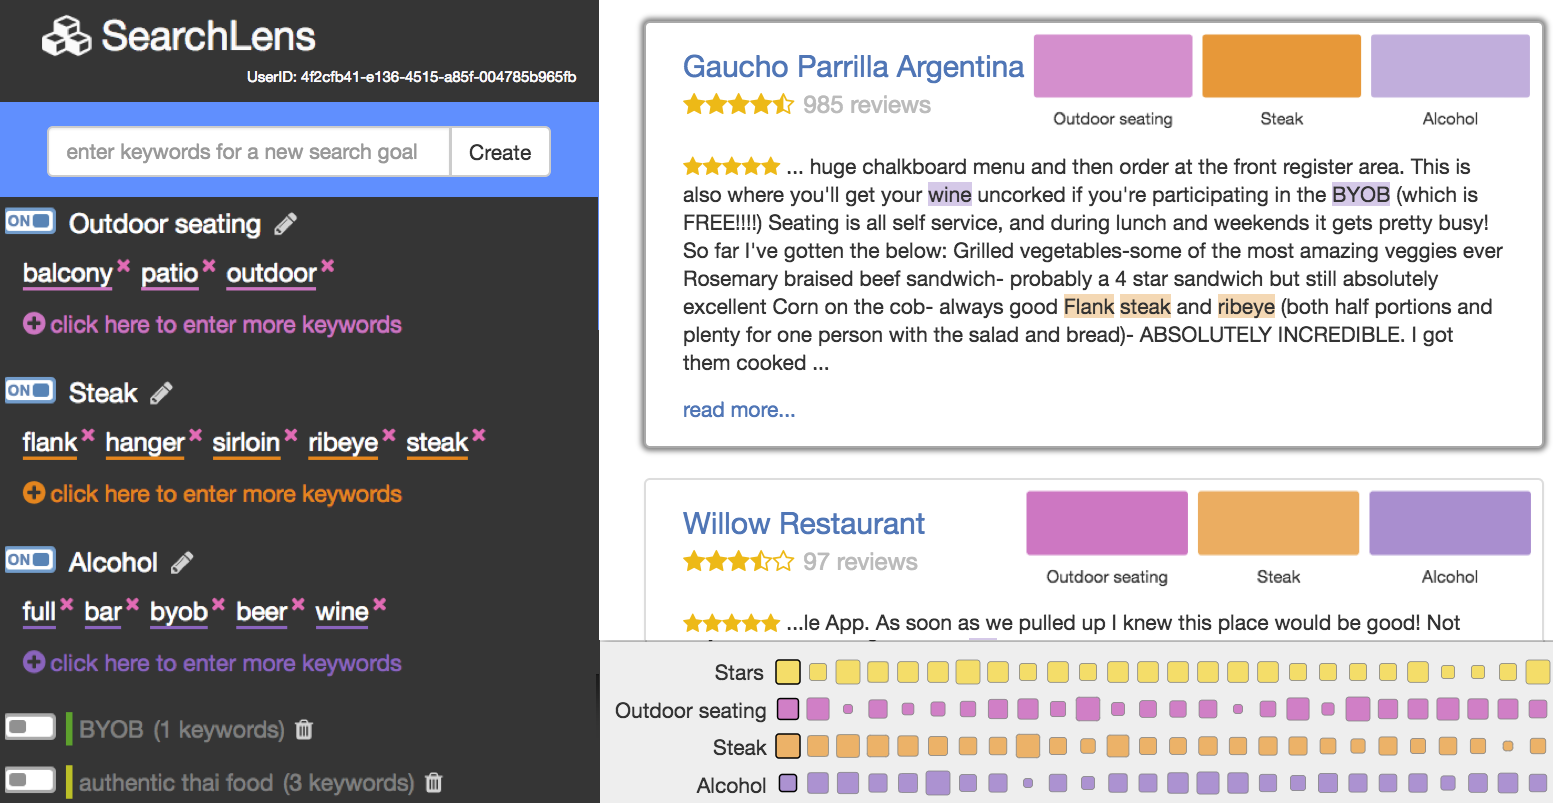
\includegraphics[width=0.8\columnwidth]{Chapters/SearchLens/figures/baseline3.png}}
    \caption[Baseline system interface for the SearchLens lab study.]{A Baseline system with topic-level visual explanation by collapsing the colored cells in each Lens and visualizing results only at the topic level.} %Unlike in the SearchLens condition, users can only explore each restaurants at the topic-level, but not the individual keyword level.}
    \label{fig:sl_baseline}
\end{figure}


\subsection{Usability Study}

The main goal of the usability study was to verify in a controlled lab environment the usability of the interface and whether the visual explanation and exploration features can provide benefits to encourage users to express their nuanced and multifarious interests. We considered these the preconditions for conducting a field deployment study to test the real-life benefits of reusable and re-composable Lenses. Therefore, we focused on the following:

\begin{itemize}
%    \setlength\itemsep{-2pt}

    \item whether the interface encouraged participants to externalize multiple interests and structure them using Lenses
    \item whether participants found the visual explanation and exploration feature to be useful 
    \item whether the added benefits of visual explanation and exploration encouraged participants to spend more effort to express, iterate, and refine their Lenses
\end{itemize}

To test the above, we compared SearchLens to a baseline interface as a between subject condition, where the detailed visual explanation and exploration features were removed by collapsing the colored cells in each Lens and visualizing results only at the topic level (Figure~\ref{fig:sl_baseline}), resulting an interface similar to the TileBars and the HotMap systems \cite{hearst1996visualizing, hoeber2006comparative}. Unlike in the SearchLens condition, users can only explore each restaurants at the topic-level, but not at the individual keyword level. Since searchers can not assign importance levels for each keyword in the baseline interface, we used the standard Okapi BM25 ranking function that weights keywords based on inverted document frequencies \cite{robertson2009probabilistic}. We chose this baseline as a more conservative test of the interactive explanation features than, for example, a comparison to Yelp or other search query-driven site (which are the implicit comparisons for the field study below).

The three scenarios for the usability study are listed below. The first scenario was designed to have both clear criteria (nice decor and good atmosphere and serves beer or wine), and an exploratory aspect (find a specific type of Japanese restaurant based on your own preferences). Scenarios 2 and 3 were designed to explore whether users would be able to reuse their Lenses for different contexts and find value in doing so. Scenario 2 had overlapping criteria to Scenario 1 (serves beer, cocktails, or wine), and Scenario 3 involved performing an identical search to Scenario 1 but in a different city.

\begin{itemize}
  
%  \setlength\itemsep{-4pt}
  
    \item \textbf{Scenario 1}: Stanley is in Pittsburgh, USA visiting some friends and he is in charge of finding a few good restaurants for the group. They are interested in Japanese restaurants. They're not familiar with Japanese food or the different types of Japanese restaurants, so it is up to you to find Japanese restaurants based on reading the reviews and your personal preferences. The restaurants should have a nice decor and good atmosphere. Some of his friends like to have a few drinks with their meal, so if the place has a bar that serves beer or wine it would also be great. Since its pretty nice out, it would also be nice if the restaurants has outdoor seating or a patio, too.
    
    \item \textbf{Scenario 2}: John is looking for good seafood restaurants in Pittsburgh, USA, particularly places that serves fresh oysters and has a bar that serves beer, cocktails or wine. Decor or atmosphere are not important, but big plus if they offer outdoor seating, for example, a patio. Some of his friends are allergic to seafood, so the place must also have non-seafood options, preferably steak.
    
    \item \textbf{Scenario 3}: (Same as Scenario 1 but for finding restaurants in Montreal, Canada instead of in Pittsburgh, USA.)
\end{itemize}

A total 29 participants were recruited from a local participant pool, where 14 participants were randomly assigned the SearchLens interface with three predefined search tasks (N=14, Age=18-61, M=28.1, SD=12.7, 7 male, 6 female, and 1 other/not listed), and 15 participants assigned the baseline interface with the same search tasks (N=15, Age=18-54, M=28.1, SD=10.7, 7 male, 7 female, and 1 other/not listed). Each participant was given 60 minutes to complete the study and was compensated 10 USD. Before conducting the three tasks, participants watched a five minute introduction video that described the features in their given interfaces, which is followed a step-by-step training where participants created two pre-defined Lenses, report the name of the third restaurant in their search results, and report which keyword is missing from its reviews. Participants finished the training steps using an average of 5.9 minutes (N=29, SD=3.8). For the main task, participants were told to spend 10 to 15 minutes on each of the three tasks listed above in order. Finally, participants answered a short post-survey where we collected their subjective opinions about the systems using 7-point Likert scales and free-form responses.


%\begin{figure}[]
%    \centering
%    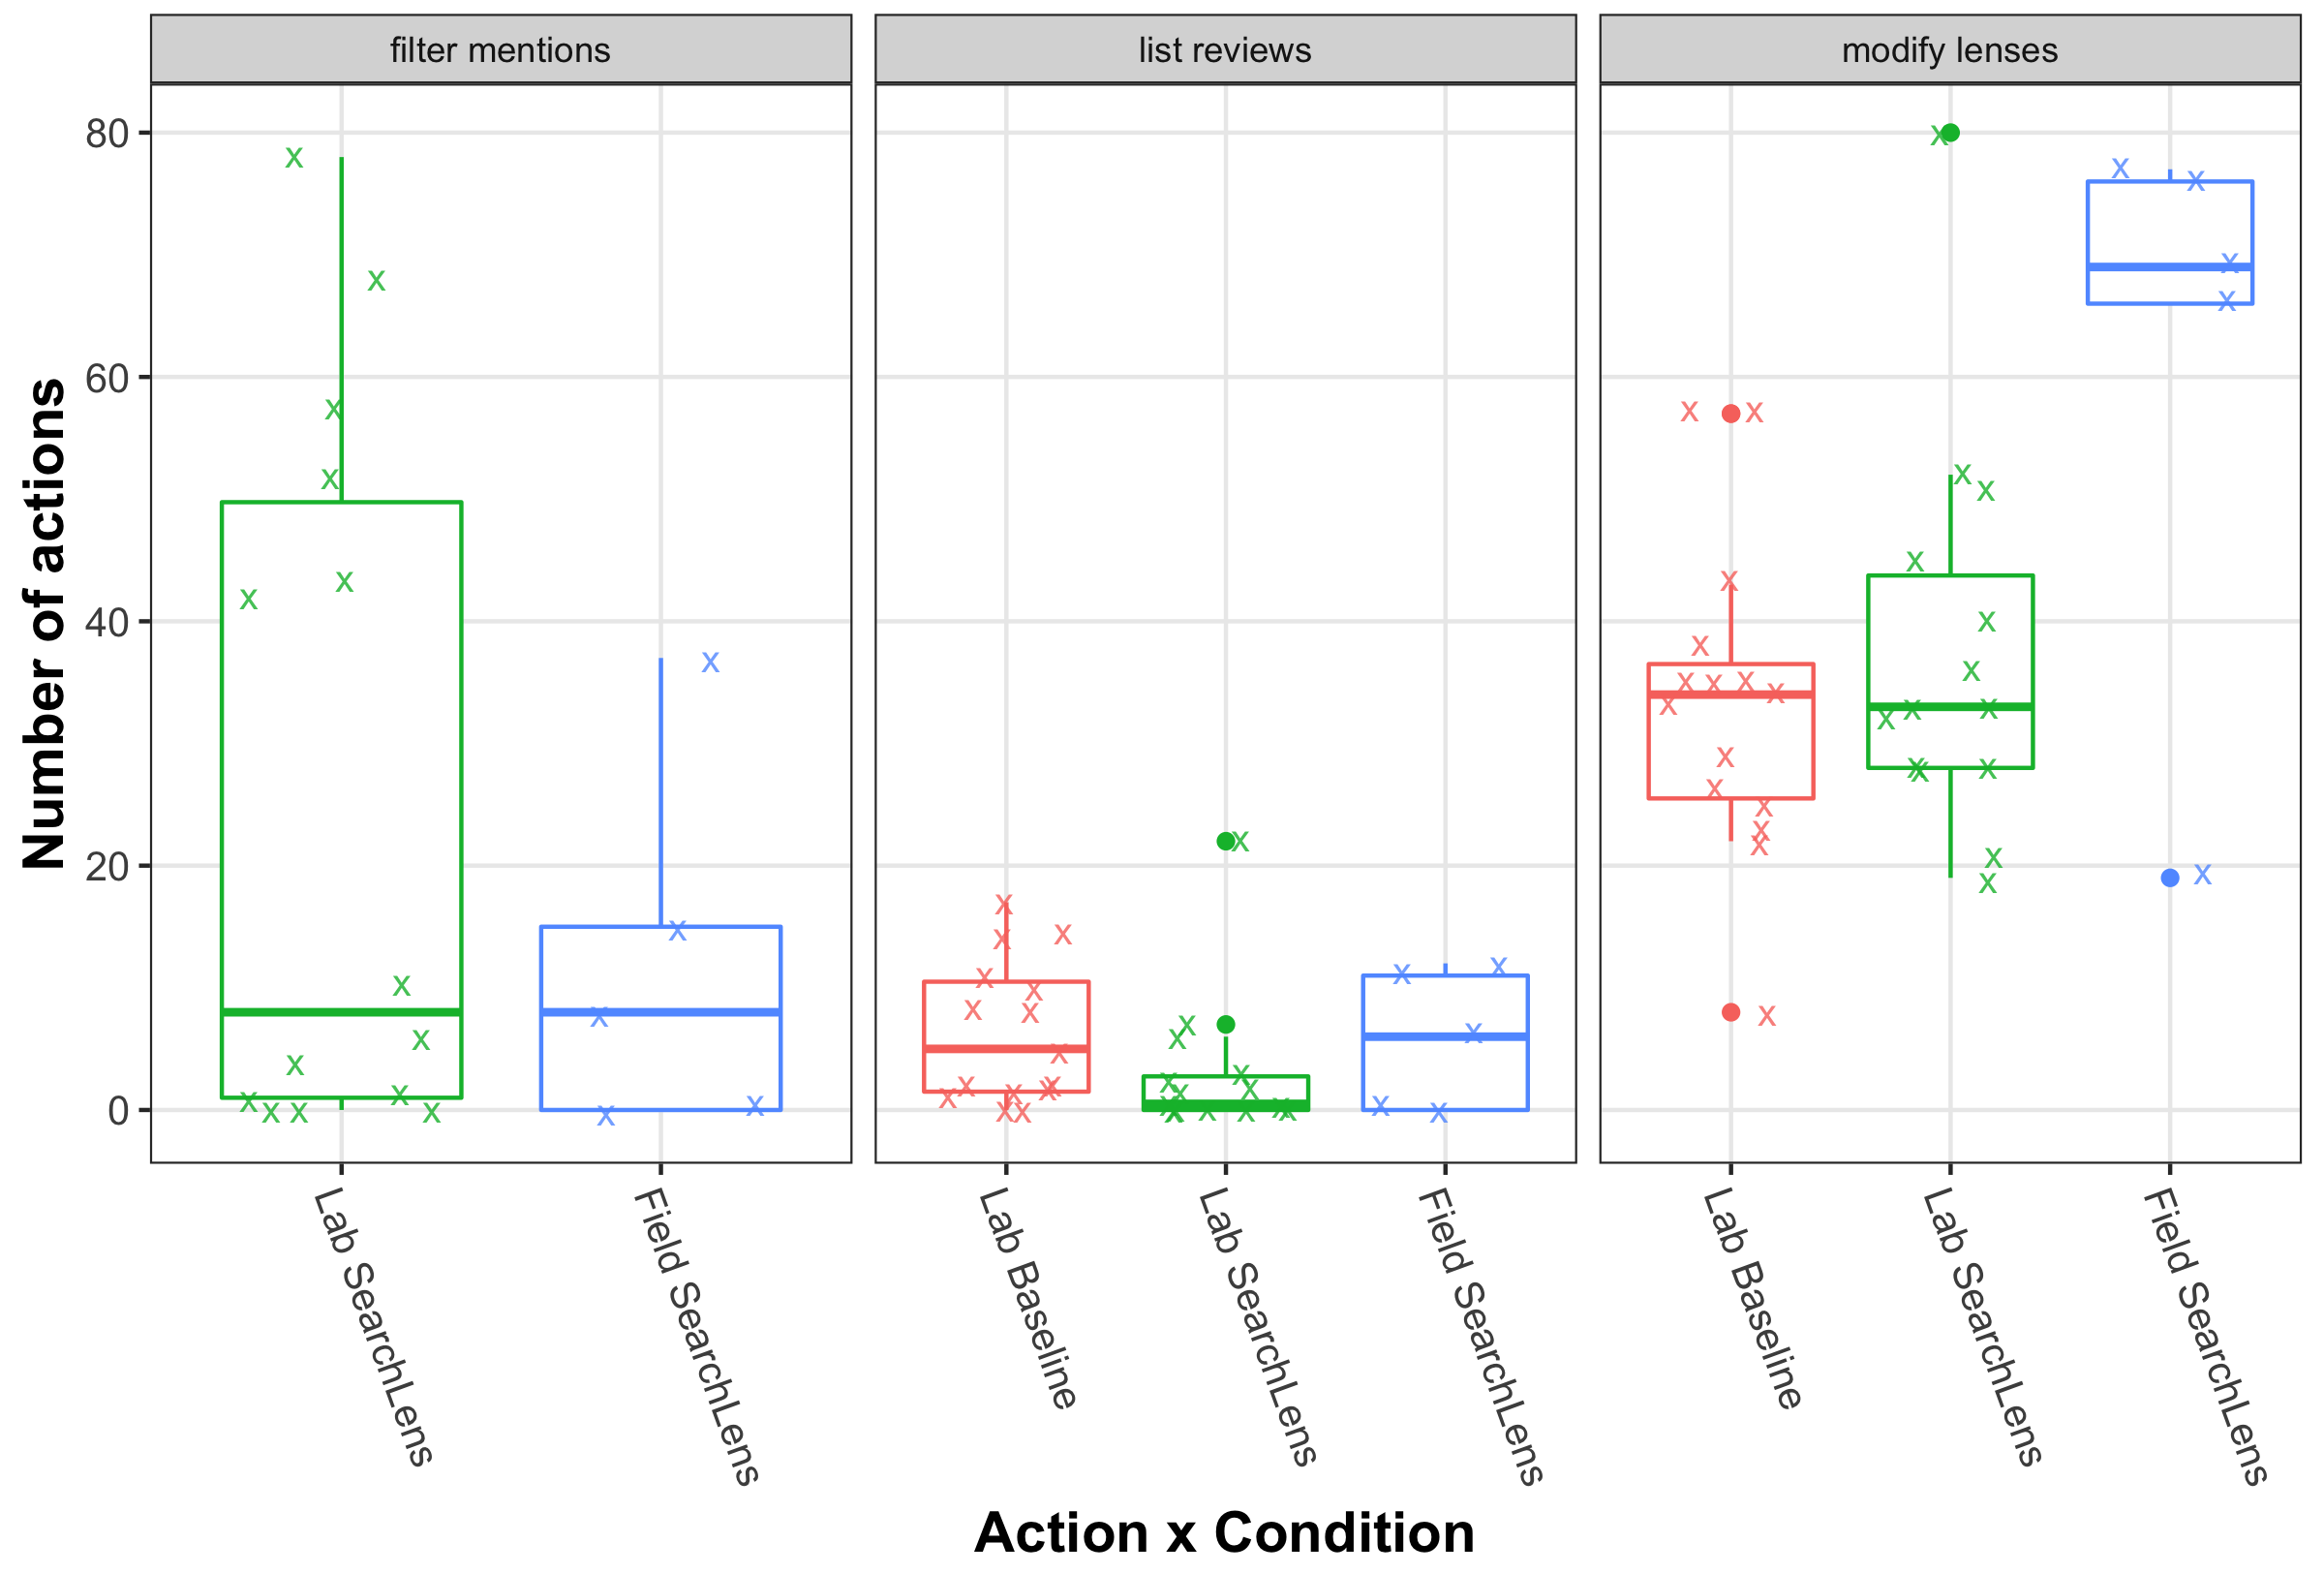
\includegraphics[width=1\columnwidth]{figures/Behavior.png}
%    \caption{Number of different action participants performed under %different conditions. Participants in Baseline relied on reading full %reviews to understand results, whereas participants SearchLens %frequently used the interactive treemaps to see keyword mentions. %Participants conducting their own tasks in the Field study tend to %refine their Lenses often.}
%    \label{fig:behavior}
%\end{figure}



%\subsubsection{Expressing Interests with Lenses}


%As a usability check, we first examine if participants expressed different interests using multiple Lenses instead of simply creating a single lens of multiple interests (analogous to a single search query bar). Figure~\ref{fig:sl_numberOfLenses} and~\ref{fig:sl_counts} show the number of Lenses each participants have saved at the end of the study, and in both conditions participants created multiple Lenses. On average, participants created 7.64 Lenses in the SearchLens condition (N=14, SD=3.65), and 6.54 Lenses in the baseline condition (N=15, SD=2.37). No significant difference was found between conditions based on unpaired T-Test (t(27)=0.94, p=0.36). This was expected since the predefined scenarios had many clearly defined criteria, and participants generally created one lens for each criteria (with multiple terms nested within lenses).

\begin{figure}
    \centering
    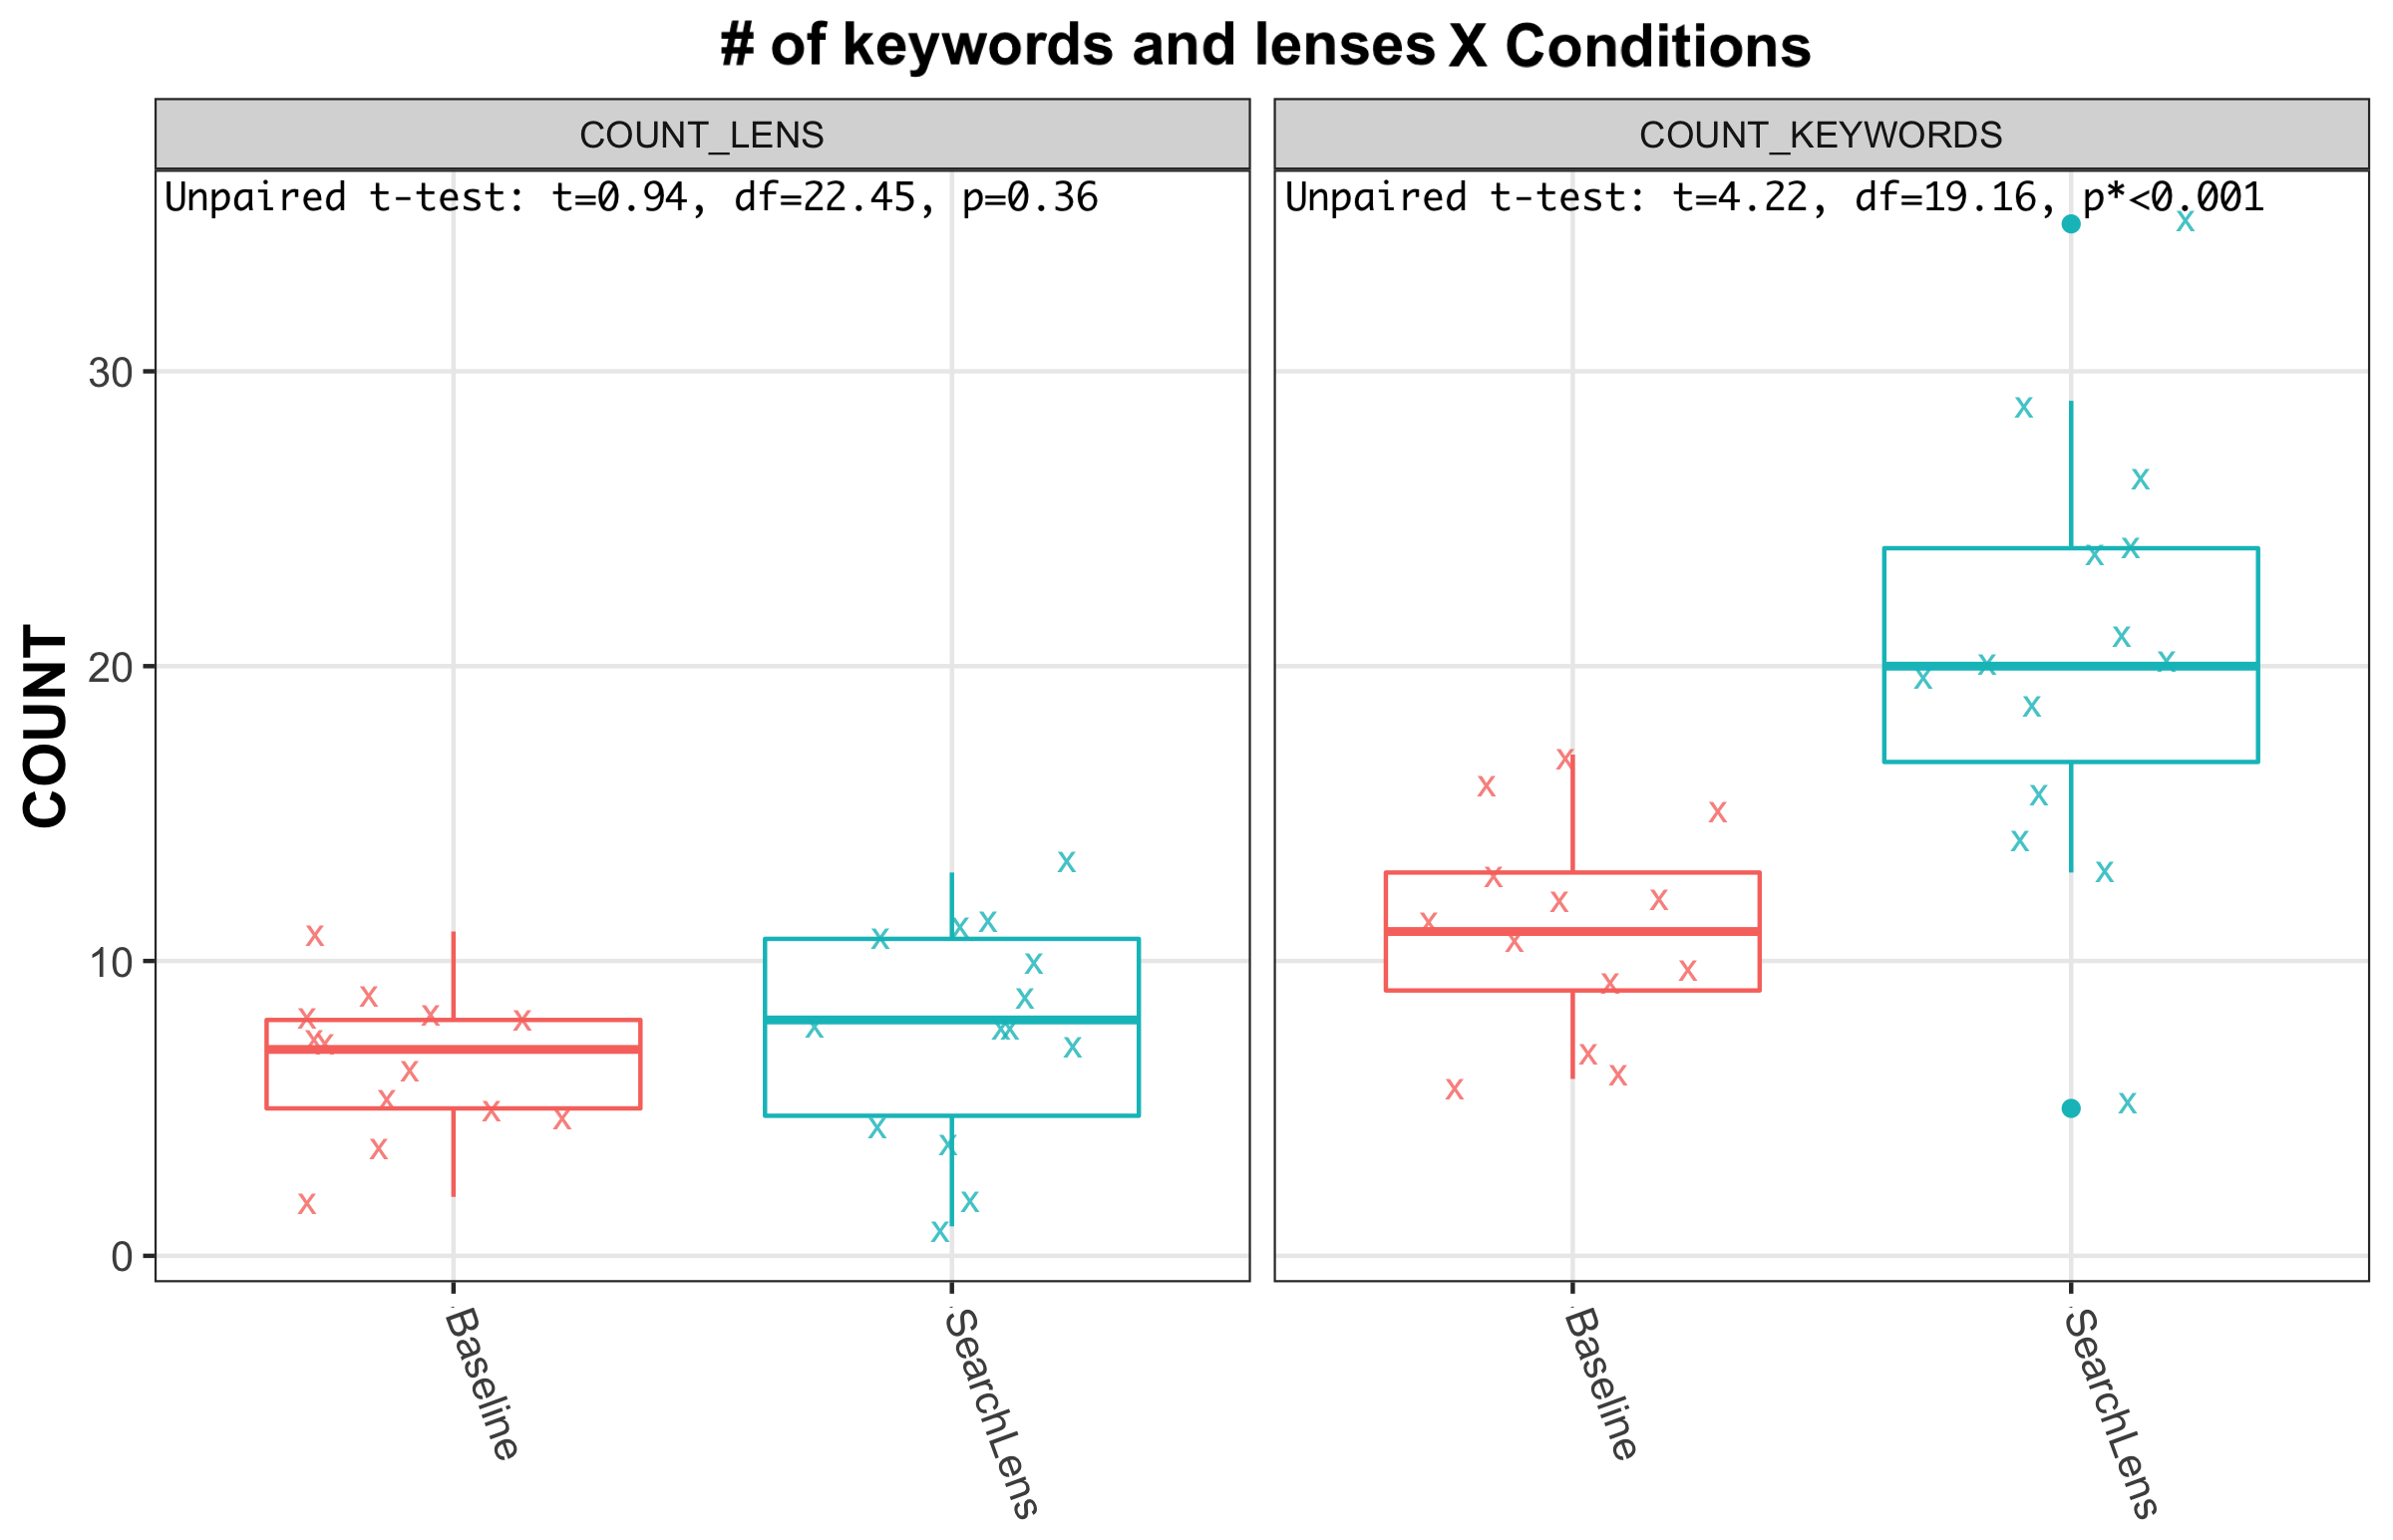
\includegraphics[height=0.45\columnwidth]{Chapters/SearchLens/figures/LensKeywordsCount3.png}
    \caption[Number of Lenses and keywords saved the participants.]{Number of Lenses and keywords saved by each participants at the end of the study. Participants in both conditions created comparable number of search Lenses, but participants in the SearchLens condition collected significantly more keywords in their Lenses.}
    \label{fig:sl_numberOfLenses}
\end{figure}

\begin{table}
  \centering
  \small

\setlength\tabcolsep{4pt} % default value: 6pt

  \begin{tabular}{ r | r l | r l |  r l }
  
	&
	\multicolumn{2}{c}{Lab} &
	\multicolumn{2}{c}{Lab} &
	\multicolumn{2}{c}{Field} \\
	
	Action &
	\multicolumn{2}{c}{Baseline} &
	\multicolumn{2}{c}{SearchLens} &
	\multicolumn{2}{c}{SearchLens} \\
    
	\hline
	
    
	 %add a new lens &
     %12.53 & $\sigma$=5.25 &
     %9.64 & $\sigma$=4.48 &
     %13.80 & $\sigma$=7.09 \\
     
	 add terms by typing &
     3.67 & $\sigma$=2.82 &
     5.50 & $\sigma$=4.86 &
     7.00 & $\sigma$=5.39 \\
     
	 add from suggestions &
	\multicolumn{2}{c|}{n/a} &
     1.57 & $\sigma$=1.99 &
     3.20 & $\sigma$=1.79 \\
     
	 add from reviews &
	\multicolumn{2}{c|}{n/a} &
     0.29 & $\sigma$=0.73 &
     0.40 & $\sigma$=0.55 \\
     
     \hdashline[1pt/1pt]
     
	 total add actions &
     3.67 & $\sigma$=2.82 &
     7.36 & $\sigma$=6.10 &
     10.60 & $\sigma$=3.71 \\
     
     \hline
     
     
	 remove a keyword &
     4.67 & $\sigma$=4.27 &
     3.50 & $\sigma$=2.79 &
     4.20 & $\sigma$=2.68 \\
     
	 adjust weights &
	\multicolumn{2}{c|}{n/a} &
     8.93 & $\sigma$=7.54 &
     12.80 & $\sigma$=7.89 \\
     
	 %reuse a lens &
     %2.00 & $\sigma$=1.85 &
     %1.64 & $\sigma$=1.28 &
     %4.20 & $\sigma$=3.96 \\
	\hline
	
	&
	\multicolumn{2}{r}{N=15} &
	\multicolumn{2}{r}{N=14} &
	\multicolumn{2}{r}{N=5} \\
	
  \end{tabular}
  \caption[Number of Lens editing actions performed under different conditions.]{Mean statistics for number of Lens editing actions performed by participants. Participants used SearchLens in the lab study more frequently add keywords to refine Lenses compared to baseline (t(27)=2.12, p<0.05). Participants in the field study conducted their own tasks. }
  \label{tab:actions}
\end{table}



\subsubsection{Results for the Usability Study}

One of our key hypotheses was that the immediate visual explanation provided by Lenses would encourage participants to express their interests and continually collect and refine those interests throughout the search process. This hypothesis appears to have been validated by the data. On average, participants in the SearchLens condition saved 20.43 keywords across their Lenses (N=14, SD=7.33), significantly more than participants in the baseline condition who saved 11.15 keywords (N=15, SD=3.58; t(27)=4.12, p<0.001). Importantly, this difference is likely not attributable to different perceptions of the task across conditions, as in both the SearchLens and baseline conditions participants generally created one Lens for each task criteria and combined multiple Lenses for each task (e.g., decor, drinks) and there was no difference between the total number of Lenses created between conditions (SearchLens: 7.6, baseline: 6.5; t(27)=0.92, p=0.36). In other words, the term-based interactive visual affordances supported by SearchLens seemed to encourage people to collect more terms indicative of their interests.

This pattern appeared to hold true throughout the search process for the iterative refinement of Lenses as well (Table~\ref{tab:actions}). On average, participants using SearchLens added keywords to existing Lenses 7.4 times (N=14, SD=6.1) while those in the baseline condition did so 3.7 times (N=15, SD=2.8), which was found to be a significant difference (t(27)=2.12, p<0.05). This suggests that the added benefits from the visual explanation and exploration feature encouraged participants to iteratively refine their Lenses and allowed them to discover useful keywords more often.

We also examined whether participants found the added visual exploration features to be useful, and how the added benefits affected their behavior. By examining the behavior logs, we found participants using SearchLens frequently use the visual exploration feature. On average, each participant clicked on 25.86 (SD=29.19) keywords to filter reviews that mention a specific keyword instead of sifting through reviews to find ones that mentioned it (Figure~\ref{fig:sl_reviews}). In both conditions, participants can also click on the name of a restaurant to see a list of reviews ranked by all active Lenses. While there is suggestive evidence that the filtering of reviews led to less use of the generic review lists, the result was not significant based on the number of participants in the study (M=6.33, 3.07; SD=5.78, 5.92; t(27)=1.50; p=0.15).

% we found participants in the baseline condition list reviews of different restaurant more often than participants using SearchLens on average , but the difference was not significant


These results suggest SearchLens allowed participants to maintain a broader search goal with multiple interests, while at the same time explore and compare different options at a finer-grain level interactively instead of sifting through the reviews of each restaurant.


%These results suggest that the added benefits of visual explanation encouraged participants to express their rich and nuance interests and also encouraged them to iteratively refine their Lenses throughout the search process.






% \subsubsection{Visual Explanation and Exploration}


%Figure~\ref{fig:sl_counts} shows the number of Lenses and keywords each participants under different conditions collected during the study. In general, participants in either condition generated similar number of Lenses. This is expected since the predefined scenarios had many clearly defined criteria. However, results suggest 

%Figure~\ref{fig:behavior} shows the number of actions participants performed under different conditions. In general, participants in the Baseline condition examined the full review lists of different restaurant more frequently then participants in the SearchLens conditions. On the other hand, participants in the SearchLens condition frequently used of the interactive treemaps to filter out mentions of different keywords, which was not available to the participants in the Baseline condition. This suggests that participants in the Baseline condition relied on listing and reading full reviews in order to understand the search results, whereas participants in the SearchLens condition frequently used the interactive treemaps to see mentions of their different keywords in the reviews directly on the search results page. Participants under the two conditions performed similar number of lens modifying actions. Figure~\ref{fig:lens_behavior} shows the average number of detailed lens modifying actions. More than 70\% of the participants in either condition reused their Lenses across condition (with 11 out of 15 participants for the Baseline condition, and 10 out of 14 participants out of the SearchLens condition). Participants under the SearchLens condition used keywords from prior knowledge by creating Lenses and adding keywords to them, but also found keywords in the reviews and used the suggested keywords. In the Field Study, we examined in more detail on how searchers utilizes different SearchLens features to refine their Lenses.


%\begin{figure}[]
%    \centering
%    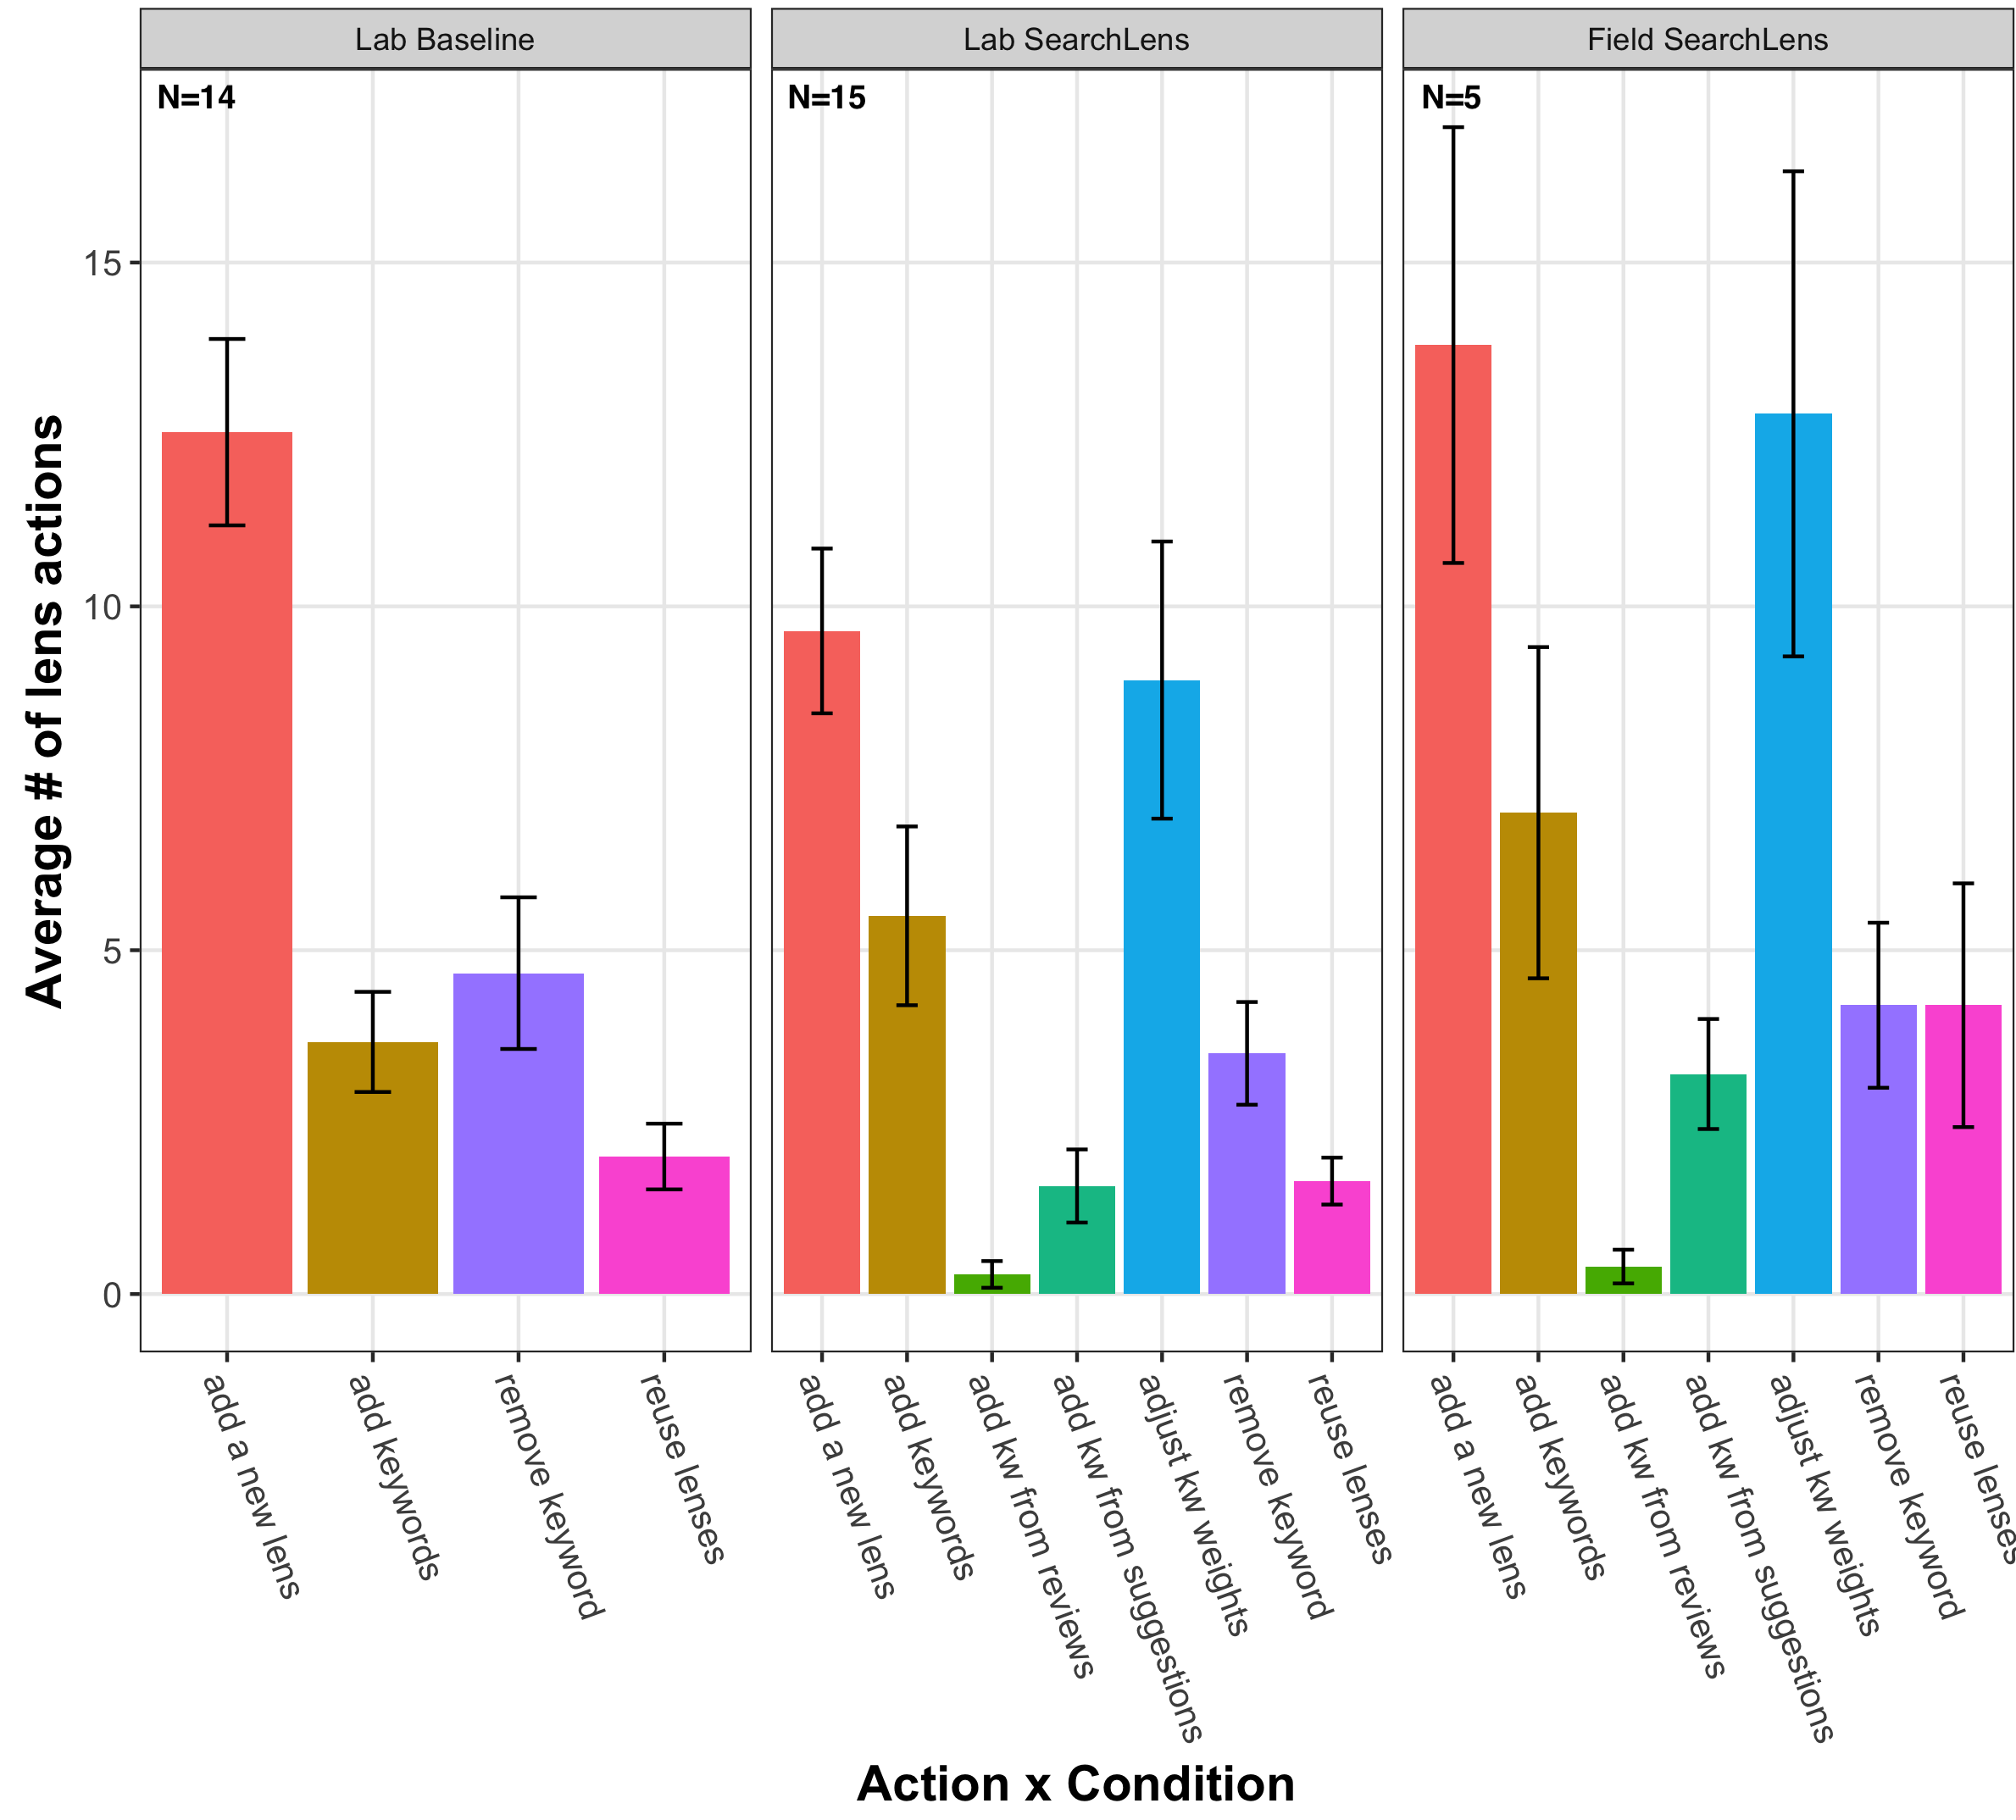
\includegraphics[width=1\columnwidth]{figures/LensBehavior2.png}
%    \caption{Average number of lens editing actions performed by participants under %different conditions. Notice keyword specific features are not available in the %Baseline condition.} %\adam{Minor: this chart is very hard to read, due to the %similar colors and overlapping text, and redundant key.  If there is time, might be %worth cleaning it up a bit.}}
%    \label{fig:lens_behavior}
%\end{figure}



%We designed the first and the third tasks to have overlapping criteria to see whether participants would reuse their Lenses created for the first task that may have been disabled while  performing the second task. Most participants in both condition re-enabled some of their Lenses that were created previously (baseline: 73.3\%, SearchLens: 71.4\%). Upon closer examination, we found that some participants deleted Lenses that were not relevant to the second task and had to recreate them for the third task, citing that they ``\emph{did not realize these are going to be useful for the third task}''. In the field study section, we further explored the benefits of reusable Lenses in real-world settings where participants conducted their own tasks using SearchLens.


% NOTE: What about combining and reusing lenses? We say that is something we wanted to look at in the usability study but I don't see anythign about it yet. Did people combine lenses?  Did they reuse their lenses when they had to do the search in a new city?


\begin{figure}
    \centering
    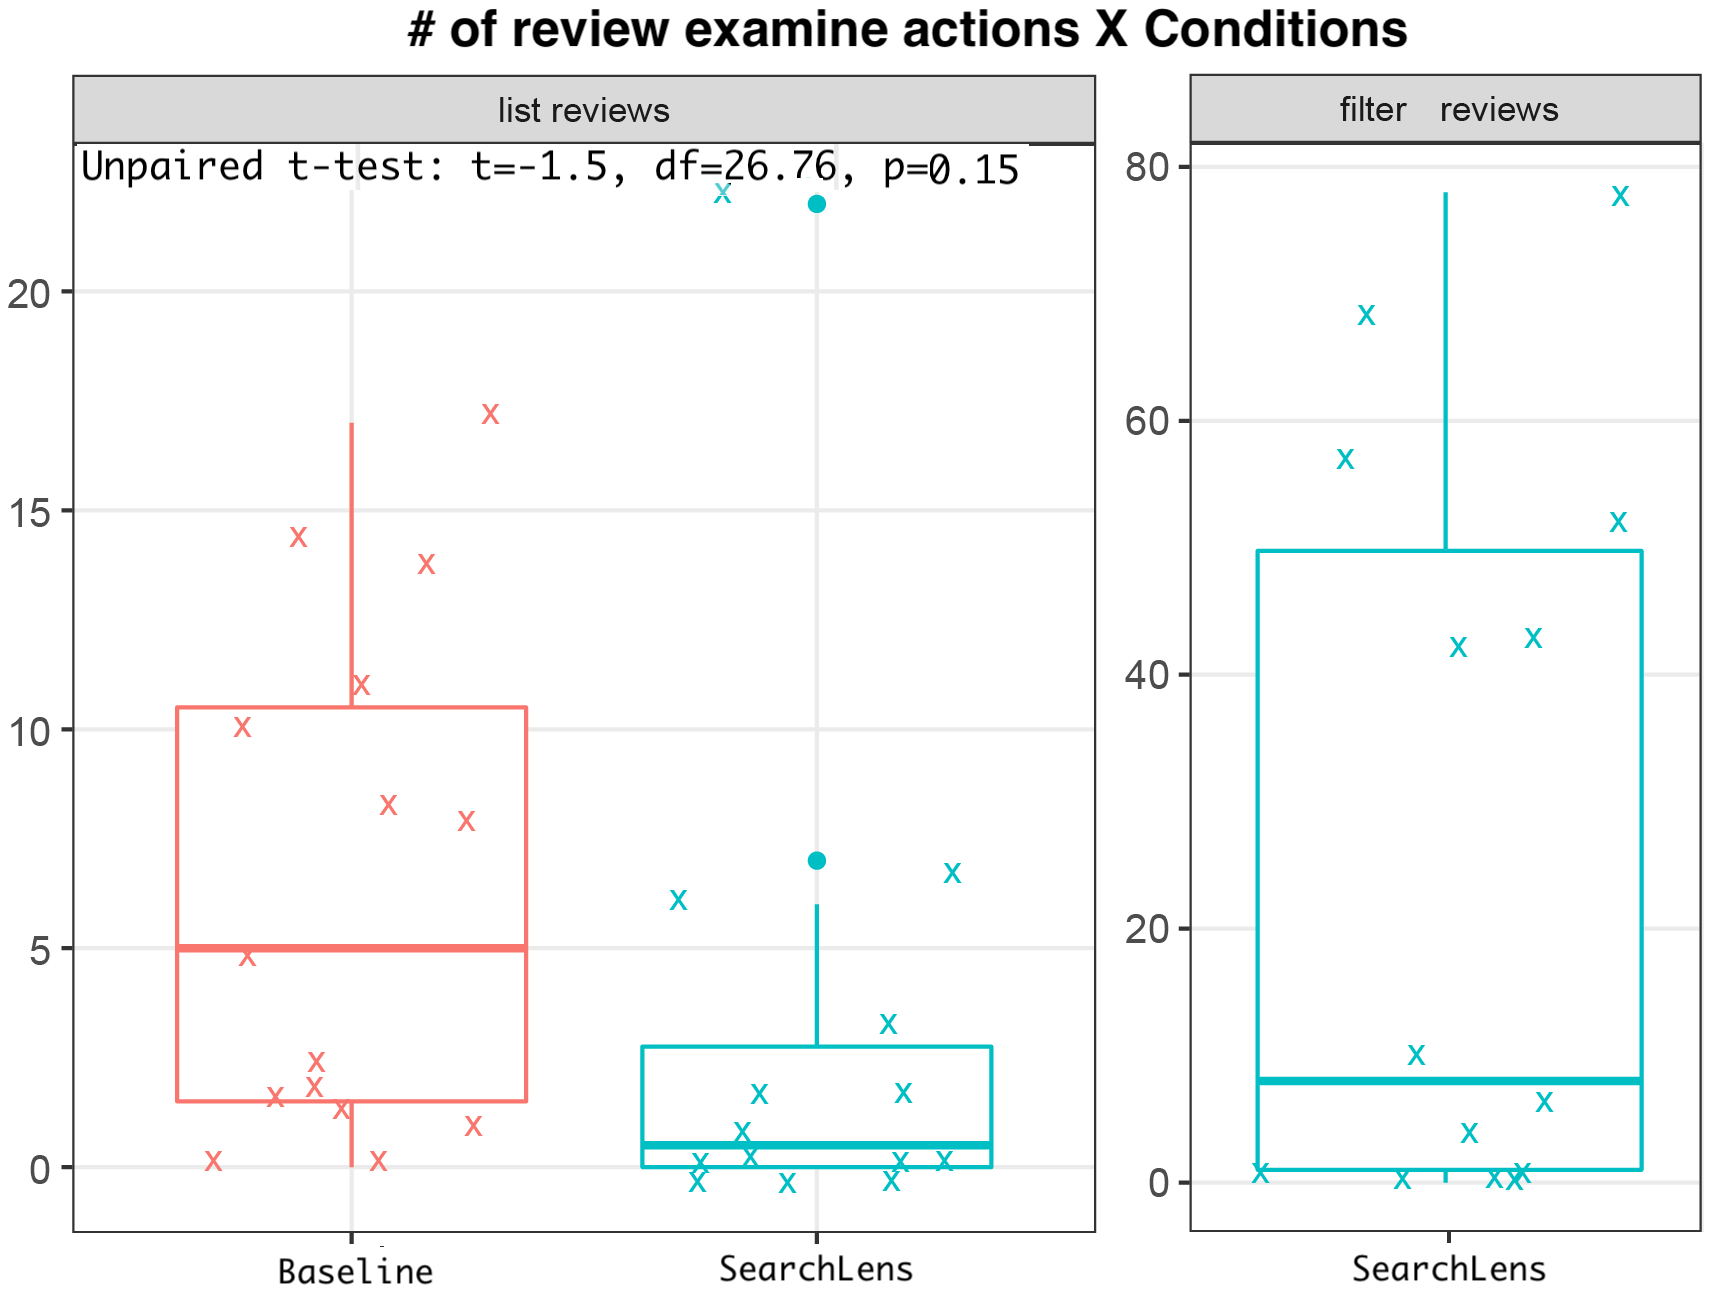
\includegraphics[height=0.45\columnwidth]{Chapters/SearchLens/figures/reviews.png}
    \caption[Participants frequently interactive with their Lenses instead of sift through reviews]{Participants in the SearchLens condition were less likely to read through unfiltered lists of reviews than the baseline condition, which was accompanied by increased use of the SearchLens-specific ability to filter reviews relevant to different keywords.}
    \label{fig:sl_reviews}
\end{figure}



\subsection{Field Study}

Our field deployment study aimed to test our idea of reusable and re-composable Lenses in real-world settings. Five participants were recruited from the first study based on their high self-reported interest in researching restaurants online and in participating in a follow up study (N=5, Age=18, 20, 22, 23, and 25, 4 male, and 1 others/not listed). The participants were given access to the SearchLens system via the internet, and were asked to use the system for at least 60 minutes in total over a three day period. Although they were free to choose from any of the 11 cities in the dataset for this study, all five participants conducted tasks for their current city.
Afterwards, they return to the lab and were given 45 minutes to finish a survey with primarily free-form questions, and were interviewed for another 15 minutes. Each participant was compensated with 40 USD for finishing the study.

\begin{figure}
    \centering
    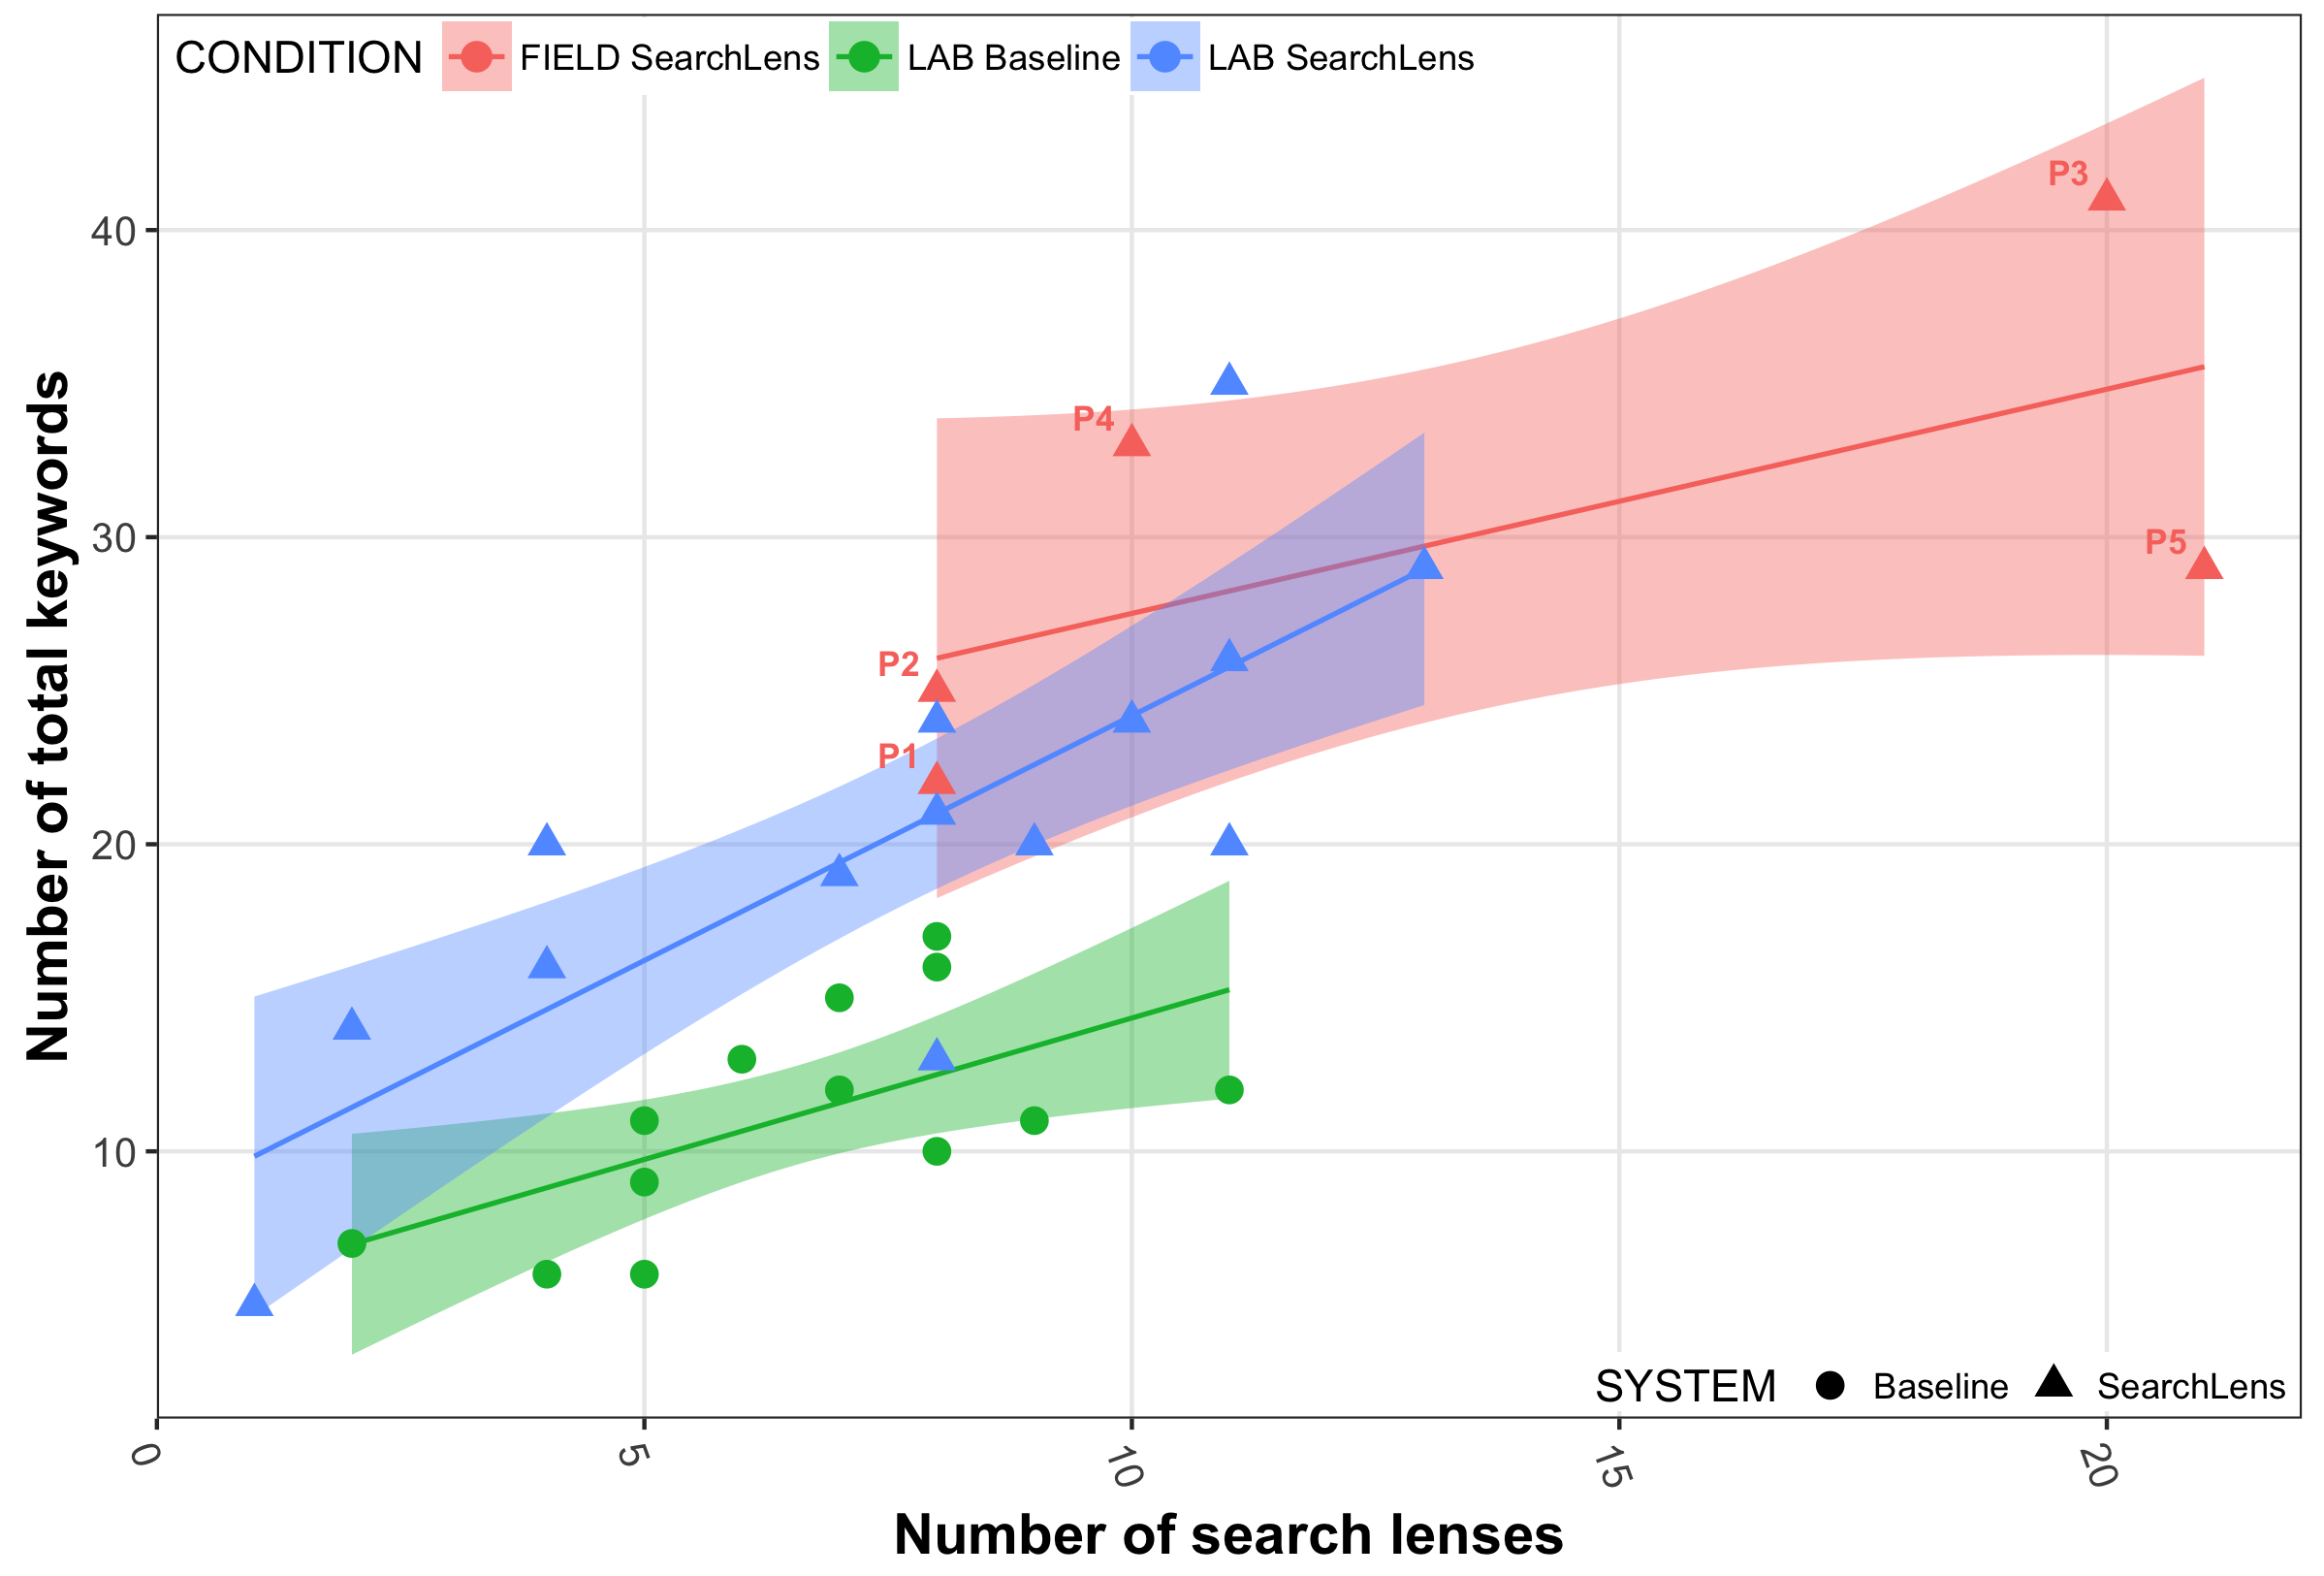
\includegraphics[width=0.8\columnwidth]{Chapters/SearchLens/figures/LensKeywordsCount.png}
    \caption[Number of Lenses and keywords under different conditions.]{Number of Lenses and keywords specified by participants under different conditions. In the lab study with predefined search tasks, participants using SearchLens (blue) created a similar number of Lenses but used more keywords than the baseline condition (green). Participants in the field study (red) conducted their own tasks.}
    \label{fig:sl_counts}
\end{figure} 


%\subsubsection{Participants and Use Cases}

Participants created more Lens keywords when conducting their own tasks comparing to participants in the lab study (Figure~\ref{fig:sl_counts}). On average, participants in the field study created 13.40 (SD=3.65) Lenses, significantly more than participants in the lab study that created 7.64 Lenses (SD=6.54; t(17)=2.46, p<0.05). They also saved significantly more keywords than participants in the lab study (lab: 20.4, field: 30.0, t(17)=2.50, p<0.05).
Admittedly, it can be difficult to measure how much time participants actually spent using SearchLens in the field, nevertheless, results suggest that participants were able to accumulate more interests Lenses over a three day period than participants who spent 60 minutes in the lab study.

All five participants conducted multiple tasks during the study. Many explored different types of restaurants that they liked in the city using multiple Lenses, using SearchLens to build \emph{``an overview interface for restaurants in the city that I might like''} (P1, P3, P4, P5). Participants also had more specific goals, including to check if there are vegan restaurants she has not discovered yet (P5), restaurants that serve bubble tea (P2), pizza places that offer Chicago deep dish-styled pizza (P3), and Mexican restaurants that has vegan options on the menu (P2).

%Below is an overview of the tasks conducted by the five participants. The number of Lenses and keywords saved by each participant is shown in Figure~\ref{fig:sl_counts}. In the next subsections, we list common use cases and strategies as reported by the participants in the interviews and post-survey:


%\begin{itemize}

%\setlength\itemsep{-2pt}
%    
%    \item \textbf{P1} conducted multiple tasks to explore different types of restaurants in the city.
%    \item \textbf{P2} used SearchLens to find Mexican restaurants with vegan options as well as places that have bubble tea.
%    \item \textbf{P3} used SearchLens to search for pizza places that offer Chicago deep dish-styled pizza, and as well as to explore the different options in the city.
%    \item \textbf{P4} was similar to P1.
%    \item \textbf{P5} was similar to P1, but specifically looked for vegan restaurants she had not yet discovered.
%\end{itemize}

%Participants P1 through P4 lived in the city for the past 3-4 years, while P5 is new to the city.

%\subsubsection{Behavior Logging}

%We recorded the behavior of our participants while using the SearchLens interface. Figure~\ref{fig:sl_counts} shows the number of Lenses and keywords each participants under different conditions collected during the study, and Figure~\ref{fig:behavior} and~\ref{fig:lens_behavior} shows the number of action participants performed under different conditions.  In general, participants in the Field Study conducting their own tasks generated more Lenses and keywords, and also performed operation on refining their Lenses. However, they were performing different search tasks and spending more time on the system than participants in the Lab Study.



\subsubsection{Refining Lenses}

While participants reported creating Lenses based primarily on prior knowledge, all five participants also reported refining their Lenses throughout the process. Several cited that the shaded cells of the visual explanation helped them quickly noticed some keywords were too uncommon, and that an important concept of interest was missing from the search results (P1, P2, P5). One also mentioned noticing and removing ambiguous keywords when using the mention filtering features (P4). Participants also learned about new keywords which they added to their Lenses, sometimes replacing existing keywords, from both the suggestions (P1, P2, P3, P5) and from the reviews (P1, P2). Interestingly, the behavioral logs (Table~\ref{tab:actions}) suggest they frequently discovered them from the systems' suggestions, indicating the value of the word2vec approach which we initially were concerned about for being noisy. This also points to potential future work in auto-suggesting Lenses which we intentionally avoided here due to concerns about agency and explainability. 

\subsubsection{Breadth and Depth}

Participants created both general, breadth-oriented Lenses and more specific, depth-oriented Lenses. P4 specifically mentioned that it was useful being able to search for different genre (i.e., American, Mexican, or Indian restaurants) and at the same time pay attention to very specific dishes (i.e., cheese steak sandwich made with chicken), while still being able to see how each result match with different things, citing that ``\emph{more specific things are hard to search for on Yelp.}'' Alternatively, P3 presented an interesting use case for deeper exploration of a specific genre, by first creating an more general Indian Food Lens, and then creating multiple more specific Lenses describing specific dishes from different regions of India, generating an overview of different styles of Indian restaurants in the city. This suggests that some users may want to create higher level groups of Lenses

\subsubsection{Reusing Lenses: Combinations and Task Resumption}

Participants reported their strategies for how they reused their Lenses, which can be broken down into two non-exclusive categories. The first use case we observed was task resumption between multiple search sessions (P1, P3, P4). Participants described having the ability to switch to a different sets of Lenses yet still keep the original Lenses for the future being useful (P3). One participant (P1) searched with a single Lens most of the time, but still cited that being able to re-enable Lenses from past sessions and to continue work on previous tasks and refined restaurants being useful. For the second use case, participants mentioned reusing Lenses in combination with other Lenses (P2, P3, P5). When asked about which of their Lenses were used in combination with different other Lenses, participants reported Lenses that concerned style and environment (\emph{Cute and Quirky} (P5), \emph{Atmosphere and Vibe} (P2, P5), \emph{Friendly Staff} (P3)), price (\emph{Inexpensive} (P2, P3), \emph{Large Portion} (P3)), and some food-related but not for a general genre (\emph{Fresh} (P2), \emph{Fast Casual} (P2), \emph{Vegan Options} (P2, P5), \emph{Strong Beer} (P3)).

\subsection{Overall Usefulness and Other Usecases}


Through the lab and the field studies, we found evidence that using user-generated Lenses to provide visual explanation for deeper exploration was beneficial and effective in incentivizing users to externalize and iteratively refine their interests using Lenses. This occurred throughout the search process almost twice as frequently when compared to participants in the baseline condition which did not include the visual explanation and exploration features (Figure~\ref{fig:sl_baseline}). As a result, participants using SearchLens created richer Lenses with nearly double the number of keywords on average compared to participants in the baseline condition. Participants also frequently used the visual explanation feature to explore the individual items in their search results, filtering reviews using different keywords in their Lenses 25.9 times on average. To test SearchLens in real-world settings, participants in the field study conducted their own tasks, and provided insights into their strategies in building and refining Lenses, as well as their strategies of composing and reusing Lenses across context and across search sessions over a three day period.

From the field study interviews, three out of the five participants said that they actually found and saved interesting restaurants during the study, and intend to visit those restaurant in the near future (P1, P3, P4). P1 in particular went to one of the restaurants he discovered using SearchLens and was happy about the visit, and P3 used SearchLens to complete a previous task, saying ``\emph{I wanted to try deep dish pizza for some time since I moved to US. Finally found one near the city. Kudos!}'' All participant expressed that they would be interested in using SearchLens in the future if available, many also cited other scenario that might benefit from SearchLens. P2 pointed to scenarios where he needed to ``\emph{find a place for many people that may want different things}'', and mentioned that SearchLens would be useful when her family visits her soon for his graduation. These results suggest that SearchLens was effective at helping users effectively find items that matched their specific interests. 

\section{Discussion and Limitations}

One limitation of the current implementation of SearchLens is its lack of ability to filter restaurants using their metadata, such as geographic location. We intentionally did not expose this information to our participants so we can focus our studies on allowing them to build personalized Lenses. However, practical systems would likely combine both paradigms to maximize efficiency. Utilizing metadata can also augment user-defined Lenses, for example, taking into account whether the a review that matched a specific Lens was positive or negative and whether the review poster's interests matched with the user's personal interests. However, the interactions between the two paradigms would require further studies. On the other hand, utilizing existing techniques for query term generalization beyond stemming or lemmatization, such as synonyms, semantic word models, or query expansion, can potentially improve recall, but their effects on the visual explanations would also require further studies.

Another obvious limitation of SearchLens it that it required more user effort upfront in order to receive the benefits provided by the system, such as reuse, explanation, and exploration. On a 7-point Likert scale, most participants from our lab study responded favorably in the post-survey to this trade-off with 64\% agreed or strongly agreed that SearchLens is an improvement to the traditional search interfaces, and another 21\% somewhat agreed with the statement, however, the long-term effect remained to be seen. One way to extend SearchLens is to combine machine learning and information retrieval approaches to reduce the effort of building Lenses, such as building interest profiles automatically, or using collaborative filtering and query expansion for expanding or inferring Lenses automatically \cite{ahn2007open,sarwar2001item,xu1996query}, or word-sense disambiguation techniques for resolving ambiguous keywords \cite{yarowsky1995unsupervised}.

Alternatively, we could also explore ways to allow users to share their Lenses with each other through explicit or implicit collaborations. For example, one participant mentioned ``\emph{It would be nice if I can see what Lenses a local person would use if I'm traveling, because I always try to ask the locals about where I should eat.}'' Allowing access to Lenses created by previous users or expert users could potentially enable expertise transfer and accumulation through continuing refinement of a set of Lenses. For example, locals and past travelers could iteratively curate a set of Lenses that leads to an interactive and explorable list of local specialties for future travelers.

Another promising direction is to more deeply explore the idea of user-generated interest profiles and how they could dynamically influence the different interfaces accessible to the user or interacting with users in more proactive ways.
Since we asked the field study participants to use SearchLens for their own tasks, most participants searched for restaurants in the city they lived in. Some participants that conducted more targeted search tasks (P2, P3, P5) mentioned that they were already familiar with most of the options in the city that fits their goals, but would still occasionally search online to see if there were new restaurants that match their interests (P2, P5).
As users continue to use SearchLens, the system will accumulate more understanding of what the users is interested in, and can potentially detect and notify the users of new information that might be of interests with high accuracy \cite{yang2006retroactive}.
Alternatively, existing users may use their repository of Lenses to explore or curate the restaurants in an unfamiliar city. Participants in the field study also pointed to the potential of Lenses being useful for other types of information and domain, including shopping (P2, P3), trip planning (P2, P5), buying a house (P2), and job hunting (P4). 


In this chapter we introduced SearchLens, a novel approach that allows users to specify and maintain their profile of multifarious and idiosyncratic interests. This enabled them to reuse and re-compose their different interests across scenarios, as well as maintaining context across multiple search sessions. To encourage users to put in the up-front effort of curating Lenses, we explored ways of using Lenses to provide immediate benefits of visual explanation and deeper exploration of search results. Across a lab and field study we observed that participants expressed their interests with significantly more query terms, and found benefits in the SearchLens approach, including being able to transfer and reuse their Lenses across contexts, being able to interpret new information that reflects their own personal interests with transparency, and working at multiple levels of specificity and hierarchy.
More fundamentally, being able to visualize and explore new information in ways that promote transparency can potentially empower users to be more aware of their online information diet. For example, as a way to manipulate their own social media feeds, and being more aware of how posts were selected or hidden. We believe SearchLens represents a first step towards a transparent and user-centered approach to addressing subjective and fragmented nature of information today.


%\section{Acknowledgments}

%This work was supported by the National Science Foundation (grants PFI-1701005 and SHF-1814826), Google, and the Carnegie Mellon University Center for Knowledge Acceleration.




%\Chapter{Intentionally Uncertain Highlighting for Foraging during Exploratory Search}{}
%\label{chap:highlight}
%

{\ttfamily
This work was previously published in ACM UIST 2016 \cite{Chang:2016:SMS:2984511.2984538} and has been adapted for this document.
}

From a better understanding of the information space (\cref{chap:alloy}) to developing personal preferences and nuanced interests (\cref{chap:searchlens}), users eventually use this understanding to collect and structure evidence to help them make better decisions. However, saving information can be cognitively costly in exploratory search scenarios because when exploring and learning the boundaries of what text may be relevant and useful later are themselves uncertain for the user. On mobile devices, this could also be physically challenging due to the small screen and font sizes combined with the inaccuracy of finger based touch screens makes it time consuming and stressful for people to select and save text for future use. In contrast to previous approaches which focused on speeding up the selection process by making the identification of hard boundaries faster, we introduce the idea of intentionally supporting uncertain input in the context of saving information during complex reading and information exploration. We embody this idea in a system that uses force touch and fuzzy bounding boxes along with posthoc expandable context to support identifying and saving information in an intentionally uncertain way on mobile devices. In a two part user study we find that this approach reduced selection time and was preferred by participants over the default system text selection method.

% See: \url{http://www.acm.org/about/class/1998/}
% for more information and the full list of ACM classifiers
% and descriptors. \newline
% \textcolor{red}{Optional section to be included in your final version, 
% but strongly encouraged. On the submission page only the classifiers’ 
% letter-number combination will need to be entered.}

\begin{figure}
    \centering
    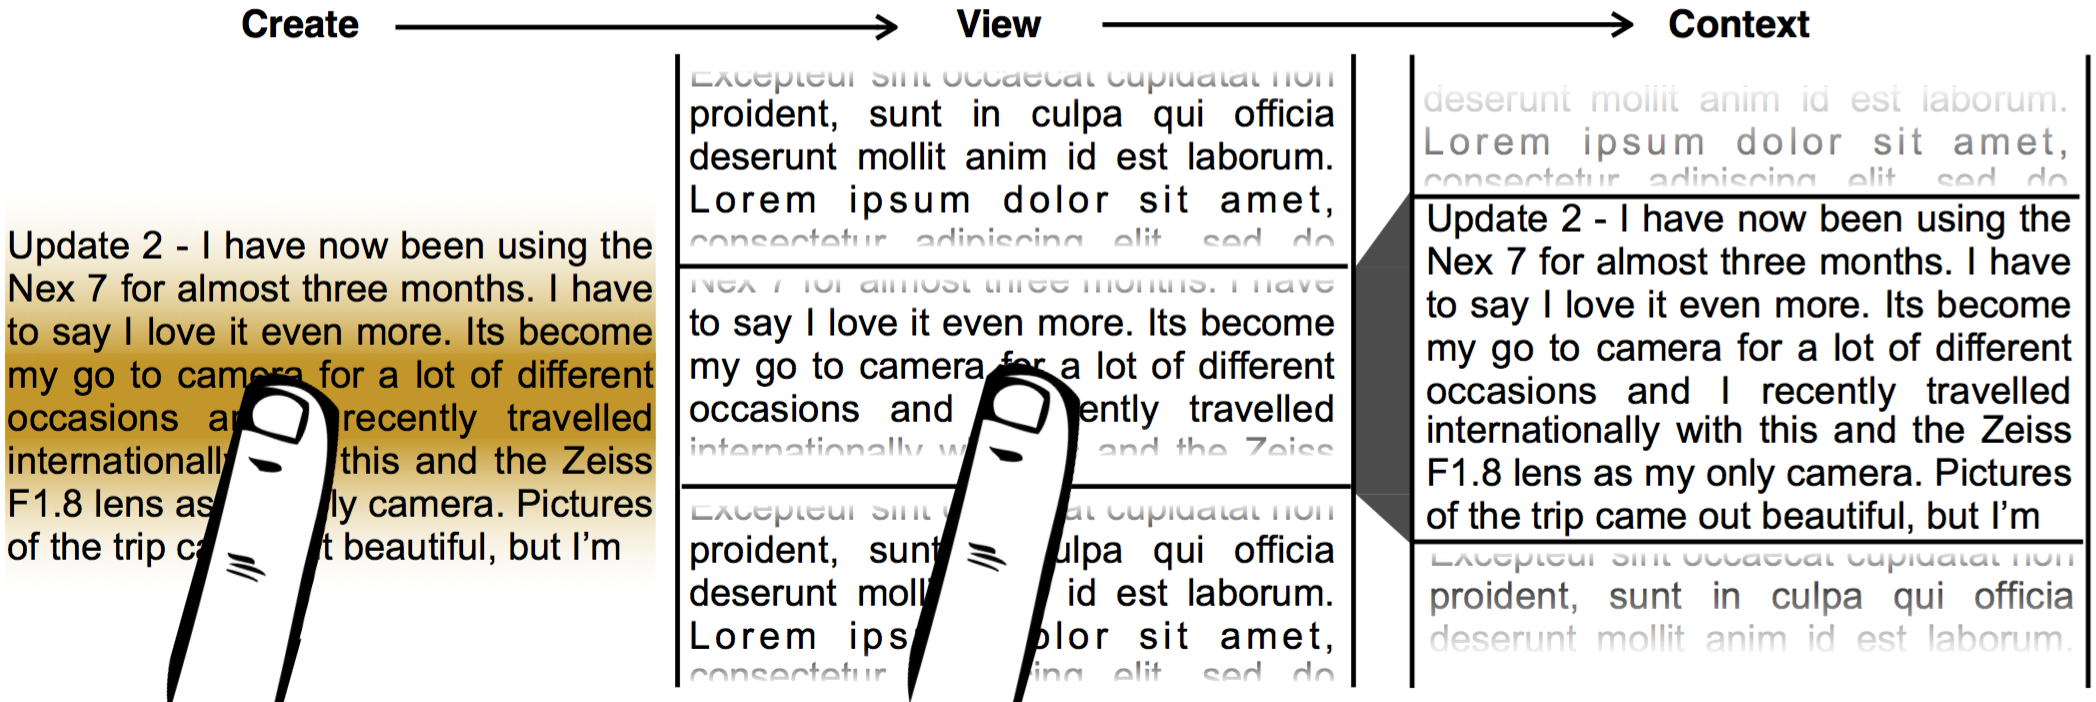
\includegraphics[width=0.8\columnwidth]{Chapters/Highlight/img/system.png}
    \caption[Fuzzy highlighting interaction and corresponding viewer]{Highlighting with intentionally fuzzy boundary and a viewer that supports resolving uncertainty.}
    \label{fig:fuzzy}
\end{figure}


\section{Introduction}

Capturing information online for later use can be especially challenging during exploratory search tasks \cite{Capra:2010:TLM:1753326.1753468}. Studies of information foraging \cite{pirolli1999information} and active reading \cite{morris2007reading} have identified the importance of collecting snippets of information while exploring and reading from multiple sources for comparison, cross-referencing, and structuring \cite{kirsh1995intelligent, adler1998diary, tashman2011active, kittur2013costs}. As reading and learning increasingly moves from handwritten notes and highlighted pages into web search and browsing, tools for supporting the curation and storage of online information have grown in popularity. For example, one well known tool for extracting snippets of information from web pages -- Evernote Web Clipper -- had over 4 million users on the Chrome desktop browser alone\footnote{http://chrome.google.com/webstore/}.

The need for reading and capturing information has expanded beyond the desk to domains where mobile devices are prevalent, such as in bed or at the kitchen table \cite{ adler1998diary,tashman2011active}. Despite this need, identifying and saving snippets of textual information remains challenging on mobile devices. Small screens and font sizes combined with the inaccuracy of touch interfaces make selecting and saving text both time consuming and stressful. To understand the prevalence of text highlighting scenarios on mobile devices today, we conducted a survey with 153 participants (age 20-59, mean 32, 60\% male, 76.5\% from the U.S.) asking for their experiences with complex exploratory searches \cite{marchionini2006exploratory} on smartphones. Our results suggest that people frequently conduct complex searches either partly (70\%) or completely (45\%) on their phones. When asked about what makes these searches difficult, near half agreed that ``\emph{Selecting part of a webpage and save it}'' is either moderately or extremely difficult, and 41\% thought it would be valuable to have a better interface for it.

Approaches to improving capture interfaces have, to date, focused on improving the speed and accuracy of specifying the start and end boundaries of the selection area. Such approaches include using bezel or multi-push gestures \cite{chen2014bezelcopy, roth2009bezel, han2015push}, autocomplete \cite{zhao2012autocompaste}, switching windows faster \cite{chapuis2007copy, faure2009power}, or leveraging the structure of the content to be copied \cite{bier2006entity, ives2009interactive, stylos2004citrine}. These approaches are well suited for fast and simple copy-paste needs, such as copying an address from one application and pasting it in another.



%However, developing a better interface for capturing information on mobile devices as people are reading also requires a deep consideration of the process that people engage in as they are learning or making sense of a new domain. 

%At the present, many smartphone information foraging support tools rely on the existing select-copy-paste metaphor native to devices. This is limiting, due to the hard boundaries imposed, and the lack of uncertain input inherent to exploration. For example, on iOS and Android devices a user initiates text selection mode by tapping and holding one finger on the screen for about 0.5 seconds and releasing their finger from the screen. Two draggable handles will then appear for specifying the start and end characters. Researchers have looked at how to speed this process up, 

%Because of the difficulties in using annotation tools in a digital medium, users often still prefer paper-based mediums for annotation \cite{tashman2011active}.
%\nathan{I changed this last sentence} 

%In these approaches, the user or system must specify hard boundaries for both ends of the selection area. 


However, in many learning and exploration tasks, people are uncertain about which and how much information to save. Early in the process, before a user has a good sense of the topic space, they might save information that later turns out to be irrelevant, or they may be uncertain about how much information on a particular page may be needed in the future \cite{kittur2013costs}. For example, a researcher might extract a particular finding from a paper early in their exploration process, only to realize later that they also need the author's statistical model from the following paragraph. Conversely, over-selecting text that does not prove to be useful later can lead to additional effort in sifting out useful information from extraneous chaff (for example, in the limit if the entire page was selected and saved then the user would have to do all the filtering again). Furthermore, forcing a user to choose hard selection boundaries requires them to carefully predict their future information need, which can involve high cognitive effort \cite{sinha2005cognitive}. Indeed, in a pilot survey, we found 11 out of 19 participants had trouble in the past identifying how much text to highlight. Additionally, 13 out of 19 mentioned that they had needed to return to a document to read additional text in order to understand the selections they created in the past. These findings suggest that these considerations are commonly encountered. Adding to the challenge, interactions for gathering information while reading need to be quick and low effort, otherwise people tend not to capture information in the first place \cite{marshall2005saving,tashman2011liquidtext,hinckley2012informal}. 

%determining how much information to save early in the process is often difficult, making fixed, context-less highlights impractical. For example, a researcher might extract a particular finding from a paper early in their exploration process, only to realize later that they also need the author's statistical model from the following paragraph. Early in the process, before a user has a good sense of the topic space, they might save information that later turns out to be irrelevant, or they may be uncertain about how much information on a particular page may be needed in the future \cite{kittur2013costs}. 

%Even more so, selection and highlighting on current mobile devices impose hard boundaries and high costs for incorrect selections. 

%which may be difficult to do if they are uncertain of the value and/or the extent of information they will need later.
%Beyond the challenge of simply selecting a region of bounded text on a mobile device, 


In this chapter, we introduce and explore the concept of intentionally supporting uncertain input in the context of selecting and saving information during information exploration on mobile devices. We investigate the idea that in contrast to more defined selection tasks (such as copying an address or phone number), precise selection may not be the most appropriate interaction paradigm for complex learning and reading tasks. In doing so we build on previous approaches that support fuzzy input, encourage lower granularity selection (e.g., lines of text vs. characters), or defer action until later \cite{schilit1998beyond,lank2005sloppy, tashman2011liquidtext,hinckley2012informal,kittur2013costs,schwarz2015architecture}
In contrast to approaches which take uncertain input and maintain its uncertainty to be resolved later (e.g., \cite{schwarz2015architecture}) in which the user intention is certain but the input is not, we suggest that there are cases in which the user intention is itself uncertain and resolving user input is inappropriate. This approach frees us to consider alternate ways to support selecting and saving information, especially on mobile devices where selecting and saving can be challenging for users. 

Specifically, we explore two ways in which we can design for intentionally uncertain input. One is to support uncertainty in the selection interface through a fuzzy bounding box. This allows a user to feel less stressed about exactly where the boundaries of their selection lie and may reduce the need for careful prediction of their future information need. Another way is to support uncertainty in retrieval by saving context around the selection area and surfacing it later. We explore the tradeoffs of these two approaches and their interaction through a controlled experimental study.
Furthermore, we introduce the idea of using pressure-sensitive touch as a new interaction approach for specifying selection boundaries. Pressure is particularly interesting as a modality because it has the potential to allow the fast selection of an area of interest while relaxing the cognitive and physical constraints of needing to specify exactly what should be saved. One potential drawback of such an approach is missing the information needed later due to inexact boundary selection, which motivated the idea of expandable context when reviewing snippets later. 
%we argue that an important user interface consideration in the learning and exploration process is designing for intentional uncertainty in the process. This uncertainty is fundamental to supporting the process of trying to identify important information that should be saved, and trying to estimate the correct context to both minimize the likelihood of missing something and reducing the amount of information that needs to be reread and filtered when using the information in the future. 
%In a larger scope, researchers have also been developing interactive systems to better support active reading and exploratory search on digital devices \cite{schilit1998beyond, tashman2011liquidtext,hinckley2012informal,kittur2013costs}. 
%In particular, Hinckley, et. al described two patterns for lowering the transaction cost of saving information while reading. First, deferring part of the actions to a later time. For example, separating and deferring annotation and categorization actions from when highlights are saved. 
%It may seem that splitting and deferring interactions could create additional cognitive cost due to lost of context, but Kittur, et al. have shown that in early stages of exploration, users often do not have enough knowledge to label gathered information effectively, and deferring parts of an interaction to a later time can actually be beneficial \cite{kittur2013costs}.
%Second, relaxing the precision of the interaction \cite{pohl2013focused}. For example, only allow users to highlight blocks of text instead of specifying character ranges \cite{hinckley2012informal}. Notice past systems have explored limiting the granularity of text selection (i.e., lines instead of characters), the input boundaries are still certain to the users at all times
%(i.e., first character of a line and last character of another), whereas in this paper, we explore the concept of uncertain input by intentionally hiding the precise boundaries from the users.
In the rest of the chapter, we will first describe the specific design of a system that embodies intentionally uncertain input in both selection (through pressure-sensitive touch selection) and retrieval of information. We then describe a two-part user study in which we investigate the performance of the two types of interfaces for a low-uncertainty task (targeted copy-paste) and a high-uncertainty task (exploratory search). 



% In two studies we found that the proposed approach is preferred over the iOS default text selection function by 19 out of 19 participants, significantly (TODO analysis) reduced user workload on interaction time and stress level during a complex sensemaking task commonly to exploratory searches. 



% \section{Related Work}

% Text selection: push-push (UIST’15), BezelSwipe (CHI’09), BezelCopy (AVI’14)

% Highlighting: ?

% Context: ?

% Uncertain input. E.g., Julia Schwarz’s work and others on touch input and interface uncertainty

% Comparing to system and many other previous approaches (push-push/bezel copy), the entire operation is done in single touch session (only one release), and potentially more time efficient. The trade off: max size / sub-line accuracy, discuss more in limitation and future work.)

\section{System Design}
In this section, we introduce a new highlighting interaction that supports intentionally uncertain selection. Our aim with this technique is to reduce the stress and increase the efficiency of saving information for future use while exploring and learning new information. The explain this interaction, we break up the process of highlighting into three separate steps: initiating selection mode, indicating the start and end points, and saving the selected text. In the remainder of this section, we will give a high level overview of the proposed highlight interaction, and then discuss the different design options we explored for each step in the interaction.

\begin{figure}
    \centering
    \includegraphics[width=0.8\columnwidth]{Chapters/Highlight/img/system2}
    \caption[Proposed interaction for selecting and saving text on force sensitive touch screens.]{Selecting and saving text using force to set the selection area (left) then sliding right to lock it.}
    \label{fig:system}
\end{figure}


\subsection{Selection Interface}

The proposed interaction is composed of three steps, which align with the above mentioned process (Figure \ref{fig:system}): 
\begin{enumerate}
    \item Users initiate selection mode with a pressure (force) touch on the general area of interest. 
    \item Once selection mode is enabled, they then estimate the amount of context needed in the future by controlling their force while moving their fingers vertically to fine-tune the start and end points. 
    \item Finally, they swipe horizontally to confirm and save the information.
\end{enumerate}

We explored three options for initiating text selection mode. One way is to use a simple touch gesture to start text selection, and swipe your finger across select text. This is analogous to using a highlighter pen to highlight text on papers. However, on a smartphone this may conflict with a number of gestures in reading mode, such as scrolling or canceling a tap on a hyperlink. The second option is to use the time dimension to initiate text selection to avoid conflicts with the reading mode gestures, such as tapping and holding at the same location for 500 milliseconds on iOS and Android devices. However, this will add an inherent cost to every highlight the user creates. 500 milliseconds might seem like a low cost if text selection is rarely needed. However, when people engage in complex sensemaking tasks, such as exploratory search, they often have the need to save pieces of information frequently in a short period of time \cite{teevan2006personal}. The third option is to use the force dimension, which is beginning to appear in mass market products, to trigger text selection. This has the benefits of having no conflict with existing reading mode gestures and virtually no time delay. Consequently, we choose the third option for initiating our text selection phase.

In designing the interaction for the selection mode, we explored four options for indicating the start and the end points. The first option is to use two draggable handles for indicating the start and the end positions, and the second option is to use the initial touch location as the start point and the release location as the end point. Both approaches are used by many current touch systems, but both suffer from the inaccuracy of finger based touchscreens (minimal target area of 44 by 44 pixels) and the small font size (default of 17 points, or 34 pixels on iOS), making it difficult to physically pin-point the intended characters. Further, the finger view-blocking problem makes it difficult to for user to do fine-grained adjustments. To avoid having the users tap on exact words or characters, we instead chose the third option, which takes the touch coordinates as the center of the selection and uses the amount of force to determine the size of the selection. We explored two sub-options for adjusting selection range based on the amount of force. We first tested using force to adjust selection range at the character or word level. However, it was difficult to keep track of the start and the end points at the same time, especially near the beginning and the end of each line. The second option is to use force to adjust how many lines are selected. This way, the start and the end boundaries have the same vertical distance to the touch location, and was much easier to keep track of at the same time when adjusting the amount of force used. We tested mapping the same amount of force used to the same number of pixel height and number of lines highlighted according to the font size of the page. The second option made the system more consistent on pages with different font sizes, and also aligns better with our design goal of correlating force with the amount of context required by the user.

Finally, for saving the selection, we explored two options. The first is to have users quickly release their fingers from the touchscreen to save the selected text. Our pilot studies showed this option to be intuitive, and often what the users try first. However, in practice this approach proved challenging as it made capturing the right selection range ambiguous, since the force dimension is also used to control the range of the selection. Similarly, in our lab study some participants encountered similar issues with the built-in text selection, and often accidentally moved the handles when releasing their fingers from the screen. Instead, in our approach users move their finger horizontally across the screen and then release to save the selected text. By using a new dimension, we reduce the chance of accidentally changing the selected range when leaving the selection mode. To reduce the number of dimensions the users need to control, we lock the selection range (both the center location and the size) once the user begins to swipe their finger horizontally. 

Previous work has shown conducting gestures in the force touched state can be laborious \cite{Lee:2014:DIT:2686612.2686702}. However, in our design, we only make use of the Y dimension movements during the selection mode, and we lock both the Y dimension and the  force dimension when the user starts moving their fingers horizontally in the saving mode (Figure \ref{fig:system}). User studies showed that participants were both able to efficiently create highlights using the proposed mechanisms, and prefer using the proposed interaction over the built-in text selection feature with draggable handles for highlighting information during a complex sensemaking task.
 

\begin{figure}[ht]
    \centering
    \includegraphics[width=0.8\columnwidth]{Chapters/Highlight/img/states.png}
    \caption[State transition diagram for the uncertain highlighting interaction technique.]{State transition diagram.}
    \label{fig:states}
\end{figure}

%\begin{table}
%    \centering
%\begin{tabular}{ l l l l }
%\hline
%Phase & X coordinate & Y coordinate & Force \\ 
%\hline
%Selection  &(not used) & selection center & selection %size\\
%Saving  & lock \& save & (not used) & (not used) \\
%\hline
%\end{tabular}
%    \caption{Dimensions used at different stages of %the operation.}
%    \label{tab:dimensions}
%\end{table}


Figure \ref{fig:states} shows the states and transitions of the proposed interaction. Notice that the proposed interaction does not interfere with common reading interactions, such as vertical scrolling or horizontal swiping (backwards and forwards buttons in Safari). In addition, the proposed interaction can also co-exist with common precise text selection methods (both commercial and academic) that are initiated with long taps or edge taps \cite{chen2014bezelcopy}. We will discuss about supporting multiple selection methods in the discussion section.

\subsection{Intentionally Uncertain Boundary}
%Admittedly, with the highlighting operation design described above, users will not be able to adjust highlight range at the character or even word level as they would using the built-in text selection features on Android or iOS. However, our pilot survey suggests that forcing people to select exact ranges for highlighting during the exploratory search process may be a source of stress, as the users can be uncertain about the amount of context needed to understand the information in the future, especially early in the process. This hints that uncertainty might be a key design consideration for highlighting new information, and lead us to believe that designing a new interaction with intentionally uncertain input at the time of saving have the potential of greatly reduce the stress and the effort involved in highlight important information during exploratory search or other sensemaking tasks involving learning new knowledge.

%\begin{figure}
%    \centering
%    \includegraphics[width=8cm]{img/fuzzy_front.png}
%    \caption{Highlighting with intentionally fuzzy boundary and precise character boundary.}
%    \label{fig:fuzzy}
%\end{figure}

We explored designing for uncertainty in two complementary ways: through a fuzzy boundary during highlighting, and through an expandable context during review. To explore uncertain input as a design consideration for highlighting, we introduced a fuzzy boundary in the selection mode (Figure \ref{fig:fuzzy}). By intentionally hiding the hard boundaries from the user, we hope to free them from engaging in the difficult task of determining exactly how much context they will need when creating highlights, and postpone uncertainty resolution until the users review the saved information with a better idea of how much context they need. To achieve this, whenever the user creates a new highlight, the system will also save its surrounding text as context. To give users dynamic access to the context when reviewing, we made a simple highlight list interface that allows the users to use force touch gesture to expand the viewport and request for more context. The idea is that knowing they will have the chance to adjust the amount of context for each highlight during the review process, it will reduce both the cognitive stress and physical interaction load of creating highlights with exact boundaries.

%\begin{figure}
%    \centering
%    \includegraphics[width=8cm]{img/viewer.png}
%    \caption{Highlight viewer that supports resolving uncertainty.}
%    \label{fig:viewer}
%\end{figure}

%In our user study, we use input uncertainty as a within-subject variable with three highlighting modes, and use the ability to resolve uncertainty when reviewing as a between-subject variable. With this study design, we can compare the users’ preferences and stress level using certain and uncertain input, as well as how having the ability to resolve uncertainty later affects their opinions about the input methods.

\begin{table}
    \footnotesize
    \centering

    \begin{tabular}{l r r r | r r r | r r r }
    
     & \multicolumn{3}{c|}{\textbf{Study 1}}
     & \multicolumn{3}{c|}{\textbf{Study 2 (with context)}}
     & \multicolumn{3}{c}{\textbf{Study 2 (no context)}} \\
    
     & Hard & Fuzzy & System
     & Hard & Fuzzy & System
     & Hard & Fuzzy & System \\
    \hline
    Mental 
    & 7.43 & 6.10 & 9.05
    & 6.78 & 5.89 & 8.33
    & 7.50 & 5.90 & 10.50 \\
    Physical
    & 7.57 & 6.00 & 9.05
    & 8.11 & 5.56 & 10.22
    & 6.10 & 3.90 & 9.20 \\
    Temporal
    & 7.90 & 7.10 & 9.52
    & 8.22 & 6.56 & 11.00
    & 6.50 & 6.60 & 9.80 \\
    Performance
    & 14.10 & 15.00 & 13.43
    & 12.44 & 14.00 & 12.11
    & 12.20 & 15.30 & 14.30 \\
    Effort
    & 8.86 & 6.76 & 11.00
    & 7.78 & 5.00 & 9.33
    & 6.20 & 6.10 & 10.80 \\
    Frustration
    & 7.43 & 5.19  & 11.52
    & 7.00 & 4.00 & 11.00
    & 5.10 & 4.80 & 8.90 \\
    \hline
    \textbf{Overall (0-100)}
    & 39.20 &31.10 & 50.14
    & 37.89 & 27.00 & 49.89
    & 31.40 & 27.30 & 49.20 \\
    
    
    & & & N=24
    & & & N=9
    & & & N=10 \\
    \end{tabular}
    
    \caption[NASA TLX scores for three highlighting modes.]{Average NASA TLX scores for three highlighting modes from part 1 of the lab study: Targeted highlighting (left), reading and highlighting with an expandable viewer (middle), and without an expandable viewer (right). Higher numbers mean higher workload or higher performance.}
    \label{tab:nasa_train}
\end{table}



\section{User Study}
We conducted a two-part lab study to evaluate three highlighting methods for saving information during exploratory search for later use: force touch with hard boundary, force touch with fuzzy boundary, and system selection. The first part of the study tested the overall interaction workload without the cognitive demands of exploratory search, while the second part added simulated exploratory search behaviors. In the first part, individuals were given articles and asked to highlight random portions selected by the system for 20 minutes. In addition to collecting data, this served to train participants to use the three modes efficiently. In the second part of the study, participants were given a complex sensemaking task involving reading multiple articles and creating their own highlights. Afterwards, they reviewed their highlights using either an interface which showed expanded context around their initial selection or that only included their original selection, and wrote a short summary integrating the content of the articles. 

We implemented the proposed technique on an iPhone 6s Plus running iOS 9.3.3 through a custom native app that uses the standard WebKit browser for the reader interface. Force touch highlighting was implemented in Javascript by accessing pressure sensor data through WebKit APIs and injected into the WebKit reader using Cocoa APIs.


\subsection{Demographic}

We recruited 24 participants from a local behavioral research participant pool. Participants ranged in age from 18 to 59. The majority of the participants were either undergraduate or graduate students, 11 female and 13 male. Participants were required to be fluent in English and use a smartphone as their main mobile phone. Based on self-reporting, 14 were Android users and 10 iPhone users. 


\subsection{Lab Study Part 1: Training and Interaction Cost}

In the first part of the study, we evaluated the interaction cost of three highlighting methods: force touch with hard boundary, force touch with fuzzy boundary, and system selection. To remove the effects of prior knowledge and the cognitive demands associated with learning new information, the system marked random portions of article in red and asked participants to only highlight the red sentences without actually reading the article. Participants were required to highlight the sentences completely without highlighting surrounding sentences in order to proceed.

\begin{figure}
    \centering
    \includegraphics[width=0.8\columnwidth]{Chapters/Highlight/img/training.png}
    \caption[Examples from the lab study]{Examples from Part 1 of the lab study, where participants were asked to create highlights covering the red lines. Pages varied in conditions including font size and page layout.}
    \label{fig:training_screenshot}
\end{figure}

Before the study began, individuals filled out a pre-survey for demographic information and how they currently used text selection or highlighting on their smartphones. During the study, participants were given a minimum of 24 pages (8 for each mode) in random order. On each page there were four highlight targets (32 for each mode). We also randomized the font sizes (30px, 38px, 47px), page layout (with/without photos), and location and size of the targets (3-8 lines).  If they finished highlighting the 24 pages under twenty minutes, more pages with random conditions were provided. Afterwards, participants filled out a NASA TLX survey for each highlight mode \cite{hart1988development} to measure cognitive load.

\subsubsection{Results}

\begin{table}
    \centering
    \footnotesize
    \begin{tabular}{r | l}
    \hline
    \textbf{Question} & \textbf{Mean[.95CI]} \\
    \hline
I find it frustrating to select text on my smartphone & 5.71[5.19, 6.23]* \\
I find it time consuming to select text on my smartphone & 5.50[4.84, 6.16]* \\
I can select text efficiently on my smartphone & 3.17[2.50, 3.83] \\
I often copy and paste text on my smartphone & 3.92[3.09, 4.74]* \\
I often highlight text on my smartphone & 3.17[2.50, 3.83] \\
I would copy or highlight text more often if it was easier to do on my smartphone & 5.79[5.26, 6.32]* \\
    \hline
    \end{tabular}
    \caption[Self-reported text selection and highlighting habits.]{Self-reported text selection and highlighting habits on a 7-point likert scale. A higher score indicates stronger agreement. N=24}
    \label{tab:text_selection}
\end{table}


Table \ref{tab:text_selection} shows the pre-survey responses from 24 participants about their smartphone text selection habits and opinions. The results show that many users find it frustrating and time consuming to use the text selection feature, and they are unable to do it efficiently or frequently. However, 22 out of the 24 participants agree that they would copy or highlight text more often if it was easier to do so. This suggests a strong need for saving information for future use on smartphone devices, and the lack of an efficient method to fulfill this need. 

When asked about the reasons for copying and pasting on their smartphones, 63\% of the participants reported copying text for later use with note taking apps or emailing themselves, and 58\% reported copying text to share information with friends via social networks, emails, or text messages. For none textual copying and pasting, 54\% of the participants reported sharing URLs with friends, and 50\% reported saving URLs for themselves. Finally, 21\% of the participants reported to not use the copy and paste feature. 


\begin{figure}
    \centering
    \includegraphics[width=\columnwidth]{Chapters/Highlight/img/runtime.png}
    \caption[Average time spent creating highlights under different conditions.]{Average time spent creating highlights in each condition: training in part 1 (left), the context condition in part 2 of the study (middle), and the no context condition in part 3 of the study (right)}
    \label{fig:highlight_runtime}
\end{figure}

Based on 1048 samples for force highlight with fuzzy boundary, 1080 samples for force highlight with hard boundary, and 1248 samples for system selection, the average time to create highlights using the three modes were 1.80 seconds, 2.77 seconds, and 6.06 seconds, respectively (Figure \ref{fig:highlight_runtime}). We analyzed these results using an ANOVA model, where duration was found to be significant different between the three conditions (F(2,20) = 18.0, p \textless  0.001). Using a Fisher LSD means difference test, we found the soft boundary selection mode was the fastest, with the hard boundary mode being slightly slower, and system selection being the slowest (p \textless 0.001). Note that these times reflect the constraint that users were not able to proceed without accurate highlighting. No significant differences were found on NASA TLX measures. In the next study, we look at how this new highlighting technique perform when users are actively engaged with the content through a complex sensemaking task. 


\subsection{Lab Study Part 2: Exploratory Information Seeking}

In the second part of the study, individuals were asked to highlight important information while researching a new topic, and to write a short summary using the highlights they created. Half of the participants were given the reviewing interface in which they could expanding context surrounding their original highlights. 

First, participants completed a pre-survey about their experiences and opinions about saving information for future use on mobile devices. Before they started on the main task, individuals were given six highlights we created from the Planet Habitability entry from Wikipedia and asked to write a short summary of the six highlights in five minutes. This was to ensure the participants in the context condition were aware that they could resolve uncertainty when reviewing their highlights when they wrote the summary. Finally for the main task, participants were given three pages to read, each containing two Amazon reviews for a different camera. Participants were told they had 15 minutes to read and highlight each source, and all three sources were of similar length, so they should spend roughly five minutes on each page. Each page required the participants to use a different method to create highlights; both the pages and modes were given in random order. After 15 minutes, participants were given 10 minutes to review their highlights, rank the three cameras, and explain their reasoning. The instructions were as follows: 

``You have a friend who is looking to buy a new camera for taking pictures of his/her young kids at birthday parties. Using the highlights you saved, rank the three cameras, and write a short summary to explain to your friend how and why you ranked them this way.''


After writing the summary, individuals answered a NASA TLX survey for each highlight mode according to when they were created their own highlights on the camera articles, as well as a questionnaire about the three highlighting modes and highlighting information in general.

\subsubsection{Results}

\begin{table}
    \centering
    \footnotesize
    \begin{tabular}{r | l}
    \hline
    \textbf{Question} & \textbf{Mean[.95CI]} \\
    \hline
Soft boundary makes it less stressful to create highlights than the other two modes & 5.89[5.25, 6.54]* \\
Hard boundary makes it less stressful to highlight comparing soft boundary & 3.00[2.25, 3.75] \\
The system selection mode is less stressful to create highlights & 2.05[1.51, 2.60]* \\
Its fun to use the force touch with hard boundary mode to create highlights & 3.58[2.77, 4.39] \\
Its fun to use the force touch with soft boundary mode to create highlights & 5.32[4.61, 6.02]*  \\
    \hline
    \end{tabular}
    \caption[Survey question about certain and uncertain boundary.]{Survey question about certain and uncertain boundary using a 7-point likert scale. A higher score indicates stronger agreement. N=19}
    \label{tab:fuzzy_survey}
\end{table}

A total of 19 individuals participated in the part 2 of the study, where 10 of them were given the highlight review interface with that supports expanding viewport for more context, and 9 of them were given a highlight review interface with static viewports. All of the 19 individuals also participated in part 1 of the study, and had twenty minutes training of the three highlighting modes.
Using a 7-point likert scale, user reported strong preference over having a uncertain input for highlighting during the complex sensemaking task of ranking digital cameras. On average, participants agrees (5.89/7.00) that the force mode with fuzzy boundary makes it less stressful comparing to force mode with hard boundary and the system selection mode, and find (5.32/7.00) using the force touch with fuzzy boundary mode to be fun (Table \ref{tab:fuzzy_survey}). When asked about which of the three highlighting mode they would use in the future if they need to read articles and learn new things on their phone, 15 of the 19 participants chose force touch with fuzzy boundary, 4 chose force touch with hard boundary, and 0 chose the system selection feature. In both conditions, only two participants chose the force highlighting mode with hard boundary, suggesting that even without the a way to resolve uncertainty when reviewing the saved information, some participants still prefer uncertain input while selecting and saving information. Below are  representative quotes from participants about the soft boundary force touch interface:

``The soft boundary took a bit of getting used to, but once I got the hang of it it made things go a lot faster. It took away the pressure of getting the exact lines right, and let my intuition take over about how much needed to be highlighted ''

``The soft boundary is my favorite, because it is the least physically taxing, least mentally taxing and if I'm going to highlight in an article it just has to be generally around what I want not perfect, so this was my favorite.''

``I hated how exact you had to be with the hard boundary.  It was just a huge pain. The soft boundary is so much better. I never realized how much I hated the generic copy and paste mechanisms. ''

We also asked the participants to fill out a NASA TLX survey for each of the three modes after writing the summary. To understand the workload effects, we utilized a generalized linear model to evaluate the differences between context vs no context, and the different modes of highlighting.  In the results of the model, context was not found to be a significant factor (F(1, 17) = 0.07, p = 0.789), however the highlighting mode was (F(2, 17) = 11.25, p \textless 0.01). Additionally, was no interaction effect between the level of context provided and the highlighting condition (F(2, 17) = 0.29, p = 0.749). In order to understand the difference between the three highlighting modes, we ran a Fisher LSD means difference test, and found both the force touch soft (t(17) = 4.66, p \textless 0.01) and the force touch hard (t(17) = 3.10, p \textless 0.01) conditions to be significantly easier at p \textless 0.01 than the system selection feature. There was no difference (t(17) = -1.56, p = 0.128) between the two force touch highlighting conditions. 

% However, the results did not show significant differences between the two highlight review conditions. 

%\begin{figure}
%    \centering
%    \includegraphics[width=8cm]{img/overall_p2.png}
%    \caption{Comparison of the NASA TLX overall score between %three highlighting modes based on all participants in part 2 of %the study.}
%    \label{fig:tlx_p2}
%\end{figure}
%

\section{Discussion}


We investigated the idea of interfaces that support intentionally uncertain input in the context of complex reading and sensemaking tasks, where precise input may be undesirable because it mismatches the high level of uncertainty in users' understanding of the topic space, leading to stress and poorer selections. To do so we developed a system in which users could highlight information on a mobile phone using force touch, and manipulated whether the boundary was hard or soft.  We also manipulated whether when they reviewed their highlights they could query for additional context around their highlights. Through a two-part user study we discovered that participants strongly preferred the force touch interaction technique with the soft, fuzzy boundary over the hard line boundary and over the default system selection with hard character boundary. We also found that both force touch highlighting approaches resulted in significantly faster selection speeds than the default system text selection.

%\nathan{I rewrote parts of this, make sure you like it} Overall, the user study was able to show the benefit of supporting intentionally uncertain input in situations where precision is actually undesirable and cumbersome. In the two-part study, we discovered that participants strongly preferred the force touch interaction techniques over the default system selection with hard character boundary. Additionally, we found that both force touch highlighting approaches resulted in significantly (\joseph{numbers}) faster selection speeds than the default system text selection.

While the force touch approach showed benefits in terms of speed, ease of use, and user preference, we also consider the drawbacks of such a solution.  We initially hypothesized that people would not like the fuzzy force touch approach if they could not query for additional context later. However, only one participant mentioned this as a negative:

``I did like the Soft Boundary better because I found it a lot less frustrating, but in the end, I think it is not as practical as the Hard Boundary just because of the accuracy level. It didn't take as much work, but I was also worried if I was able to include everything I wanted to include in the highlight.''

Instead, it seemed that most users appeared to adjust for the soft boundary, for example by oversampling the selected text, and were not bothered even when they were not able to adjust context posthoc.  This suggests that the soft boundary interface may be useful even with existing review interfaces that do not support posthoc adjustment, but also lead to concerns that the proposed technique promotes mass highlighting, which past work has suggested to have negative effects on learning \cite{peterson1991cognitive}. By examining the highlights participants created in the second part of the study, we found the proportion of highlighted words did not significantly differ across conditions with absolute numbers trending against the hypothesis: On average, participants highlighted 27\% of the camera reviews under the force touch with hard boundary condition, 20\% with the system selection, and 19\% with force touch with fuzzy boundary, suggesting the fuzzy boundary did not encourage mass highlighting. We analyzed these the highlighted information proportions with a generalized linear model, and did not find the highlighting condition (F(2,13) = 2.39, p = 0.111), context condition (F(1,13) = 0.51, p = 0.487), nor their interaction (F(2,13) = 0.38, p = 0.687) to cause any significant variation in the amount of text highlighted. 

Another non-optimal case for this approach is when the task is a strict copy-paste task in which hard boundaries are important, for example copying a telephone number or an address.  
 Therefore, supporting both scenarios the same devices seems crucial for the proposed technique to be practical, and
  past work has also pointed to benefits of supporting both fine-grained and coarse-grained manipulations with fully-engaged interactions and casual interactions \cite{pohl2013focused}.
 We believe there are at least two possible interaction paradigms for supporting multiple selection interactions at the same time that can be explored in future work: 1. \emph{Independent sets}. The proposed method does not conflict with many existing academic and commercial techniques (e.g,. edges of a screen\cite{chen2014bezelcopy} or long taps) which do not currently make use of the pressure dimension. Thus each method could be implemented and the user could choose which to use given their current need. 2. \emph{Sequential sets}. The two approaches could be combined by performing a fuzzy selection first and then allowing the users to switch to a precise selection mode to further adjust the boundaries (e.g., using force to select an area including an address, which brings up optional handles to trim off text around the address).


A final limitation we will discuss is the size of the selection area, which is currently fixed to a maximum limit. One participant mentioned this as a concern, stating: 

%\blockquote{``I really liked both of the force touch modes but at times I felt that the maximum force touch highlight box size was not large enough. They were much easier to use than the system mode but also less precise, which is a sacrifice I would be willing to make simply because it's much less fickle to use.''}

``I really liked both of the force touch modes but at times I felt that the maximum force touch highlight box size was not large enough.''

Informally, we noticed that we were able to select reasonably accurately when testing the system with larger size selections than explored in the study. However, it is possible that with a sufficiently large selection jittering from finger tremors or inaccuracy may become problematic. Exploring smoothing and transformation functions from the pressure input to match human cognitive expectations and physical capabilities is a fruitful area of future work. Furthermore, there is an interesting edge case when the selection consists of the entire screen, and whether users consider this a phase transition that should mean the entire page should be saved or simply the highlighted area. Appropriately addressing this concern is something that future work will be need to answer.

Although we have focused here on the particular use case of highlighting information on mobile devices, it is possible that the idea of supporting intentionally uncertain input may have broader implications. The most obvious inference is for information exploration on desktops: although mice or pens as pointing devices make selecting much easier, the cognitive uncertainty of where the boundaries should be drawn remains. There may be other kinds of tasks in which uncertain input may be supported better as well. For example, many applications and operating systems require files and folders to be named as soon as they are created, which can lead to inconsistencies between the name generated early on and what the contents of the file and folder end up being later, with resulting problems in refinding and organizing that information. More generally, we believe that uncertainty in user input should in the future be treated as a design feature, not only a limitation.


%\section{Acknowledgments}

%This work was supported by NSF grants IIS-1149797, IIS-0968484, IIS-1111124, and the Yahoo! InMind Project.


% Balancing columns in a ref list is a bit of a pain because you
% either use a hack like flushend or balance, or manually insert
% a column break.  http://www.tex.ac.uk/cgi-bin/texfaq2html?label=balance
% multicols doesn't work because we're already in two-column mode,
% and flushend isn't awesome, so I choose balance.  See this
% for more info: http://cs.brown.edu/system/software/latex/doc/balance.pdf
%
% Note that in a perfect world balance wants to be in the first
% column of the last page.
%
% If balance doesn't work for you, you can remove that and
% hard-code a column break into the bbl file right before you
% submit:
%
% http://stackoverflow.com/questions/2149854/how-to-manually-equalize-columns-
% in-an-ieee-paper-if-using-bibtex
%
% Or, just remove \balance and give up on balancing the last page.
%



\Chapter{Weaver }{Entity-Centric Foraging across Webpages in the Browser}
\label{chap:weaver}

The previous chapter explore ways users can express and maintain their different criteria for selecting restaurants, and use them to visualize a review dataset and compare different search results. This chapter focus on supporting global context so that users can better evaluate their different options as they encountered them on different webpages. Unlike in the previous chapter where the evidence (i.e., reviews) were already recognized by the different restaurant entries on Yelp, this chapter instead support users' general browsing of different webpages using their browsers. This is enabled powering browsers with modern named entity recognition and linking algorithms, allowing us to identify the same entity mentioend across users' browser tabs.

As people research online to plan trips or shop for new products, they encounter many entities (e.g., attractions, products) and collect evidence across webpages to make informed decisions (e.g., reviews, listicles). Current browsers treat entities on each webpage independently of other pages, making it difficult for users to keep track of what they are interested in and why. We introduce Weaver, a novel browser add-on that weaves pages together through common entity mentions to support sensemaking across browser tabs in the context of trip planning. When users open a webpage, Weaver ``infuses'' it with evidence from other information sources relevant to entities on the current page. When users save notes, their notes are ``diffused'' across other pages that mentioned the same entity. We compared Weaver to a baseline and found participants utilized Weaver to gather nearly three times more evidence collected across significantly more webpages, and synthesized evidence to support decision making with lowered interaction costs.


\section{Introduction}


\begin{figure}
    \centering
    \frame{\includegraphics[width=1\textwidth]{Chapters/Weaver/main3.png}}
    \caption[An overview of the Weaver browser add-on.]{An overview of the Weaver browser add-on. Weaver identifies and highlights entity mentions on webpages [A,B] to indicate additional information is available. Highlights in red [B] indicates users had previously interact with the entity. Hovering an mention [B] brings out its corresponding entity card [E] as an overlay, with relevant information ``infused'' from other pages and knowledge bases as \emph{mentions}. Users can also save notes or selected sentences [F1] to a card as \emph{clips} [F2]. Saved clips are then automatically ``diffused'' to other webpages that mentioned the same entity. Users can also create categories [D] and drag the card under them. Finally, the Map view [C] shows its location in context of previously saved entities.}
    \label{fig:main_fusion}
\end{figure}

Whether planning a trip to a new city, figuring out which camera to purchase, or researching the different treatments for a medical issue, learning and searching for information online has become the most common way that people make sense of the world today \cite{mar2006exp,pirolli1999information}. People spend a significant amount of time exploring available options and gathering evidence about them that are scattered across multiple webpages in order to make informed decisions.  Estimates suggest that up to 33\% of the time spent online \cite{mar2006exp,kellar2007field,rose2004understanding}, or, as of 2009, around 24 billion hours per year in the US alone, are spent doing this type of aggregation and synthesis \cite{forrester}. 

We believe this problem of synthesizing information across sources is increasingly relevant as online information and misinformation (such as fake news and shill reviews) continues to expand. Past studies have shown users rely on aggregating from multiple sources in order to verify online information as credible and make decisions \cite{fox2000online,cotten2004characteristics,racherla2012perceived}, but the process can be ``tedious and cumbersome'' leading to ``opening several tabs ... and then manually switch[ing] between them while trying to remember information on different pages'' \cite{greis2017increasing}.  Anecdotal evidence for this can also be seen in the rise of aggregation-based sites such as Metacritic or Wirecutter, but such aggregators cannot cover all decision making scenarios nor able to take into account the personal context and goals of different users. In our own informal interviews on people's past experiences with trip planning and examining their notes, we also discovered similar needs and challenges -- they compared a large number of options based on evidence gathered from multiple sources, but struggled with managing large numbers of options and sources. 

In this paper, we focus on the domain of travel planning, because it has a number of characteristics that make it a good task to test new sensemaking and exploratory search approaches. For example, while it does not require a strong domain knowledge, useful information is often scattered across many sources; there is a strong degree of contextualization and personalization needed (e.g., traveling somewhere with kids is very different than without); and evidence such as reviews can be noisy and subjective \cite{zhang2012human,chen2015tripplanner}. Consider for example planning a trip to a new city: there may be hundreds of possible restaurants to dine at, attractions to see, and places to stay, each with corresponding evidence about its suitability for an individual's goals and preferences. Evidence about each of these options is often spread out across multiple search results, such as Yelp or TripAdvisor reviews, top ten lists, travel blogs, or forum posts. It can be a challenging process of intense cross-referencing and note taking to synthesize this evidence and to record how it meets a user's goals, with little scaffolding or intelligence built into the browser \cite{o1996towards,marshall1999introducing,tashman2011liquidtext,bianchi2015designing}.

%As the amount of user-generated content on the internet continues to grow, supporting users to benefit fully from large repositories of rich evidence is likely to become increasingly important \cite{mudambi2010research,gan2012helpfulness}.

%to To make an informed decision Cross-referencing evidence across these sites and In order to compare different options and make informed decisions, users need to cross-reference a large number of webpages to synthesize evidence about each potential option.  However, this process of intense cross-referencing and note taking can be disruptive when reading and consuming information \cite{o1996towards,marshall1999introducing,tashman2011liquidtext,bianchi2015designing}, and is poorly supported by current browser and note taking interfaces. As the amount of user-generated content on the internet grows, supporting users to benefit fully from large repositories of rich evidence is likely to become increasingly important \cite{mudambi2010research,gan2012helpfulness}.

Currently, such intelligence primarily takes the form of entity-centric approaches in search results interfaces \cite{guo2009named,lin2012active}. These approaches include showing entity cards with rich attributes for entity-bearing queries \cite{miliaraki2015selena,bota}, listing related entities as suggestions for subsequent queries (such as listing actors when searching about a movie) \cite{blanco2013entity,bordino2013penguins,klouche2015designing}, or extracting factual attributes about or relationships between entities (such as the director of a movie) \cite{balog2010overview,cheng2007entityrank,D15-1038}. While these approaches can efficiently provide factual and structured information about entities in search interfaces (such as when figuring out the location of a restaurant), they provide little support for the complex sensemaking situations described above, when there is no single objective answer that can be surfaced in a search results page (such as figuring out which city to visit for a vacation).

Instead of using entities as an answer or endpoint to a user's information needs at the query and retrieval stages, here we explore the idea that entities can also be useful during the reading and note taking stages by acting as the fabric connecting different information sources and use them to scaffold the user's mental model in complex exploratory search tasks. Leveraging entities has the potential to enable deeper and more fluid interactions with online information by focusing on meaningful concepts as the units of a user's externalized mental model rather than webpages. Furthermore, recent advances in entity linking algorithms have been particularly promising in bringing the ability to better understand web content to the browser where users read and learn from individual webpages \cite{spotlight}. For example, leveraging common entities mentioned across webpages to provide a sensemaking structure for users conducting complex exploratory searches and foraging across multiple webpages.

Specifically, in this paper, we explore a new paradigm for interacting with unstructured and subjective evidence about entities while reading and foraging from many webpages in exploratory search tasks. Since the user's personal evaluation of subjective information and how it meets their goal is critical in this situation, our design goal was to help the user to see scattered evidence about an entity in one place while also attaching personal notes and web clippings. These together serve as a way to build up an external mental model and track search progress.

To investigate our entity-centric approach, we developed a prototype browser add-on called Weaver. Weaver allows users to keep track of information scattered across multiple sources by ``infusing'' evidence about an entity from other information sources (webpages and knowledge bases) to the webpage the user is currently reading. It also ``diffuses'' users' thoughts about different entities across webpages where the same entities are mentioned for future reference and to accumulate more evidence. In our user study, we tested how participants utilized our entity-centric approaches while conducting a complex exploratory search task, focusing on whether Weaver allowed them to explore, gather, reuse, and accumulate evidence about entity options across multiple webpages. To control for task complexity, the primary domain on which we aimed to test Weaver was a pre-defined travel planning task (described in the Study Design section). With 24 participants and a baseline interface as a between subject condition, we found that participants using Weaver collected nearly 3 times more evidence across 60\% more pages while simultaneously being more selective in the options they explored. Furthermore, we describe qualitative evidence of the value in infusing of evidence from other webpages and diffusing users' notes across webpages. Finally, we discuss implications for the design of future intelligent interfaces that can better understand the information being consumed by their users by taking advantage of advances in natural language processing to support online sensemaking in various scenarios.




\section{Related Work}

\subsection{Sensemaking and the Web}

The importance of sensemaking and complex exploratory search on the web has been studied in depth by many researchers. Past work have identified a persistent challenge that valuable information for many topics is scattered across many different sources that are independent of one another and incur a high cost for bringing them together \cite{bhavnani2005difficult,mar2006exp,marshall1999introducing,kittur2013costs}. Theories of sensemaking suggest several cognitive tasks involved that could be supported through novel interactive tools, ranging from finding potentially relevant items, to triaging items based on reliability and relevance, to collecting evidence relevant to each item and organizing items into categories or structures \cite{russell1993cost, takayama2008tracing, hearst2013sewing}. We draw on these theories to select the set of cognitive tasks we are interested in supporting through entity-centric interaction approaches, which are typically complex and about synthesizing information, rather than simple fact-finding tasks \cite{mar2006exp, white2006supporting}.

\subsection{Recognizing Entities in Text}

Significant research has gone into entity-centric approaches for improving web search results pages due to the ubiquity of entities in online sensemaking. Researchers have found that entity-bearing and -category queries accounted for up to 85\% of web search traffic \cite{guo2009named,lin2012active}. This has led to significant academic and commercial efforts devoted to building large-scale entity databases (such as DBPedia \cite{dbpedia}, Yelp\footnote{http://yelp.com}, and Google Places\footnote{https://developers.google.com/places/web-service/intro}), and significant research on ways to identify entity mentions in plain text \cite{spotlight} and using them to enrich search interfaces. This involves both recognizing the same entity mentioned in different surface forms (e.g., MoMA and Museum of Modern Art) and resolving ambiguous surface forms to the right entity based on its surrounding text. Major threads of research that uses entities to improve search interfaces includes showing entity cards for entity-bearing queries \cite{bota,miliaraki2015selena}, answer factual questions  \cite{D15-1038}, and showing related entities as query suggestions \cite{blanco2013entity, bordino2013penguins,klouche2015designing}. We build on these recent advances in entity recognition and large-scale entity databases, but instead of focusing on the search interface and simple navigation we investigate the less-explored design space of supporting complex sensemaking across webpages opened in the browser through entity-aware interactions.


\subsection{Weaving Together Scattered Information across Sources}

Due to the scattered nature of information on the Web \cite{bhavnani2005difficult}, research has explored ways to connect relevant information distributed across different webpages. One set of top-down semantic web approaches involve incentivizing content publishers to provide machine readable annotations, such as using semantic web markups \cite{karger2004haystack, berners2001publishing,berners2001weaving}. However, such approaches have often failed to gain momentum due to issues such as a lack of available end-user tools that can consume these annotations \cite{whatwentwrong}. Alternatively, researchers have built bottom-up systems that exploit detecting entity mentions in articles, and used them as anchor points to connect to other information sources to enhance the reading experience. For example, Wikify identifies entity keywords in articles and creates hyperlinks to their Wikipedia entries for navigation \cite{mihalcea2007wikify}, and Experience-Infused
Browser links entity mentions in articles to past social interactions (such as emails) for making ``serendipitous connections'' \cite{hangal2012effective}.

Our approach is inspired by these bottom-up approaches in the context of recognizing entities mentioned in webpages opened in the browser. However, our work differs in several important ways: 1) instead of surfacing simple facts or links to articles or emails, we focus on providing context for people to understand complex information spaces; 2) we support the transition from viewing context to saving information; and 3) we propagate saved information to all other instances that entity is shown, allowing users to build up an entity-based mental model of the space.

%Instead of navigating users to a separate page, we used an in situ design that allowed users to hover over an entity mention to bring out its entity card \emph{infused} with relevant information extracted from other information sources. In addition to information from external knowledge sources (such as Wikipedia), we also used the entity cards to show relevant information extracted from other opened webpages that also mentioedn the same entity for lightweight cross-referencing.


\subsection{Note Taking and Saving Information Online}

Collecting information online during complex sensemaking tasks can be costly for the users, requiring them to cross-reference between pages and their notes in order to gather all the evidence. This frequent context switching between different documents and taking notes can be distracting, and even prohibitive for users to investigate deeper or to take notes in order to avoid disrupting the flow of reading \cite{o1996towards,marshall1999introducing,tashman2011liquidtext,bianchi2015designing}.

On one end of the spectrum, research has focused on allowing users to extract and save structured information from webpages more efficiently from a single document using end-user programming \cite{thresher,huynh2005piggy,dontcheva2006collecting,dontcheva2007relations} and interaction techniques \cite{bier2006entity,stylos2004citrine}. Our work is motivated by these studies highlighting users' desire to collect information about entities, but instead of focusing on structured and objective attributes we are interested in additionally gathering descriptive and subjective evidence, such as how a restaurant is described in a top ten list. Furthermore, many of the approaches above define patterns for extracting multiple entities from a single page, whereas we are more interested in finding evidence related to entities across multiple pages where the structure of those pages might differ significantly.

On the other end of the spectrum, researchers have also explored using in situ interfaces, such as sidebars or on page annotations, to reduce the costs of switching between reading and note taking and collecting from multiple information sources \cite{romat2019spaceink,tashman2011liquidtext,notetoself,van2011finders,schraefel2002hunter}. Our work is also situated in this thread of research on reducing the costs of switching and sensemaking. However, instead of persisting notes on individual documents, our approach persists notes on individual entities which may then appear across multiple documents. 

%Unstructured note taking approaches also run into challenges with scaling for reusing and organizing large collections of saved notes.  For example, a prior system, NoteToSelf, reported that their participants relied on skimming or targeted search using keywords from memory for re-finding previously saved notes, which led to a large portion of user notes rarely re-accessed nor deleted \cite{notetoself}. Fundamentally, note taking software treats options mentioned on webpages and users' notes about them as independent, and cross-referencing between webpages and their notes to accumulate evidence for the same options can be incur high costs. In this work we explore an entity-centric approach that connects different webpages and users' notes through common entity mentions, allowing us to automatically resurface previously saved notes as they became relevant to users' current reading.




\begin{figure}
    \centering
    \includegraphics[width=1.0\columnwidth]{Chapters/Weaver/expanded.png}
    \caption[Expanded view for an entity card.]{Expanded view for an entity card showing information \emph{infused} from external knowledge sources (Yelp and Wikipedia), user's notes, and evidence of the same entity from other webpages in the exploratory search task. See Figure~\ref{fig:main_fusion} for the non-expanded view of an entity card.}
    \label{fig:expanded_fusion}
\end{figure}


\section{System Design}

We introduce Weaver, a novel browser add-on that uses an entity-centric approach to facilitate sensemaking across webpages in exploratory search tasks. 
Unlike previous approaches that focused on either enriching search results pages \cite{syed2017optimizing,miliaraki2015selena}, saving information from individual documents \cite{tashman2011liquidtext,thresher}, or providing separate note taking interfaces \cite{dontcheva2007relations}, we focused on supporting sensemaking across multiple information sources by weaving them together through common entity mentions. This allows users to both evaluate potential options with more context and re-access previously saved information about an option with lowered effort.
Figure \ref{fig:main_fusion} shows an overview of how an exploratory searcher planning a trip might use Weaver. Weaver provides users a lightweight overlay interface embedded on and synced across webpages opened in different browser tabs, allowing users to make quick and lightweight cross-referencing without switching between tabs, windows, or applications.

The two core components of Weaver scaffold sensemaking through entities in two primary ways, which we introduce as ``\emph{Infusion}'' and ``\emph{Diffusion}.'' First, when users open a webpage from their search results, the system ``infuses'' the webpage with relevant snippets about mentioned entities from other webpages in their search results and external knowledge sources to help users cross-reference and evaluate newly encountered options. Second, when users save notes or extract content from a webpage, the system ``diffuses'' them to mentions of the same entities in other webpages of the same task, allowing them to easily access previously saved information without having to switch to and search through their notes a separate interface. In the next subsections, we will first describe in detail both Infusion- and Diffusion-based features, a project overview interface, and finally describe how entities were automatically identified and linked to external knowledge bases.

\subsection{Infusion: Gathering Evidence from other Webpages}

One significant challenge in making sense of a given topic on the internet is that relevant information is scattered across multiple places, and it is difficult to find those places and to synthesize what they say. Doing so is valuable in understanding the popularity and prevalence of a given option (e.g., how often a restaurant is mentioned in lists of top restaurants, what are the various lists of top restaurants) as well as the context and potential biases in how it is described (e.g., is it suitable for a date night, are the pages it is mentioned on reliable). Instead of using them at only the beginning on search results pages, entities could provide a scaffold for improved in situ interactions throughout the browsing process to help users more quickly get a sense of the popularity and context of different options without going to all the different pages on which they are mentioned, as well as providing ``pivot points'' to see what other sources mention an option.

For example, in Weaver, a user planning a trip to a new city can open an article from a travel blog and see all the destination and restaurant mentions highlighted in yellow. Hovering on a attraction surfaces contextual snippets from other webpages that also mention that attraction, so the user can understand its relevance to their own goals without interrupting their flow of reading (Figure~\ref{fig:main_fusion}, B and E). Other sources of information can be brought in and surfaced at the same time, such as Yelp review scores and Wikipedia descriptions. By infusing this information using the entity as a pivot, it is possible that users could both reduce the number of items they need to keep track of (by filtering out non-matching items earlier) and better understand the context of the items they do keep. Meanwhile, the number of sources that mention the item provides implicit feedback as to its popularity within the searches the user has made; their URLs may provide context as to the reliability of those sources; and they may provide additional sources for finding information about other restaurants if they mention a restaurant the user knows they like. 

%A common activity in complex exploratory search involves collecting information from multiple sources and make informed decisions.
%Our preliminary survey, as described in the Introduction, showed that 88\% of participants ``use information from multiple webpages to verify uncertain information.'' % removed from intro
%echoed by our preliminary study described in the Introduction in which 88\% of participants reported that they typically gather evidence from multiple sources ``in order to verify uncertain information.'' %Similarly, 83\% reported that they would typically perform at least 4 searches to gather information when planning a trip, and 50\% would spent at least 4 hours searching when purchasing something important or expensive.
Weaver supports this need by ``infusing'' entities mentioned on a page with context pulled from other webpages mentioning the same entity or entries in external knowledge sources (in our current implementation, DBpedia and Yelp). When users open a webpage, entity mentions that were recognized by Weaver are highlighted with a half-height yellow highlight (Figure \ref{fig:main_fusion}, A) to indicate they have information from other sources. By hovering over an entity, a user can see an ``entity card'' (Figure \ref{fig:main_fusion}, E) which displays those sources and relevant information (e.g., number of stars on Yelp, paragraphs from other websites in which the entity was mentioned) which a user can use to gain context about the entity beyond the current webpage \cite{bota}. To read the mentions, the user can click on the icon of each external source to see an extracted snippet. Alternatively, the user can also expand the Card to see a larger view (Figure~\ref{fig:expanded_fusion}), showing all mentions, multiple images, and a map of the location using metadata from Yelp and/or DBpedia. 

%As a running example, a user planning a trip to a new city might open an article from a travel blog and see all the destination and restaurant mentions highlighted in yellow by Weaver. As the user reads the article, he or she finds a highlighted restaurant and the author recommended it for reasons that also fit our user's personal interests. However, instead of relying on this single piece of evidence, the user hovers over the restaurant name to query for its entity card for additional information. The entity card contains Yelp review scores, Wikipedia description, and a list of relevant snippets from other webpages from the user's previous searches. After reviewing these information, the user drags the entity card under the restaurant category created previously. 

\begin{figure}
    \centering
    \frame{\includegraphics[width=1\textwidth]{Chapters/Weaver/project2.png}}
    \caption[An project overview page created by one participant.]{An project overview page created by one participant after searching for 50 minutes, containing entities saved under different categories, text clips from multiple webpages, and typed notes. Custom cards were created, including one for a kayaking tour that was not available on Yelp and DBpedia. The entity cards were scaled for clarity in this figure.}
    \label{fig:project_fusion}
\end{figure}





\subsection{Diffusion: Propagating Notes to other Webpages}

After using ``infused'' context to judge the relevance and suitability of options (i.e., entities), users often need to keep track of and organize the options they found valuable. At the same time, users may evaluate newly encountered options against ones they have already saved. Typically, this happens by copy-pasting or typing entity names and notes into a separate interface, for example a separate document or email or note taking software (e.g., Evernote). Researchers have tried to lower the switching cost involved in this interaction \cite{o1996towards,tashman2011liquidtext}, for example, by adding a sidebar to the browser for taking free-form notes \cite{notetoself}. However, in the cases when the user encounters additional evidence about an option they already have information about, they need to re-find it in the external system before being able to continue. This high interaction cost can be prohibitive as it lead to disruptions of user's flow of reading \cite{chang2016supporting,tashman2011liquidtext,o1996towards,marshall1999introducing}.

Weaver addresses this challenge by ``diffusing'' notes that users associate with an entity to all other webpages in the project that also mentioned the same entity, reducing the need for user-driven re-finding. Continuing with our running example of trip planning from the previous subsection, imagine that after the user reviews the information in a restaurant entity card, he or she decides to take notes and save the restaurant for future reference. To do so, the user can add various levels of annotation to the card, including just ``hearting'' it to save it in the Saved Cards view as uncategorized  (Figure \ref{fig:main_fusion}, top-left corner of E), typing notes about reasons for saving it (Figure \ref{fig:main_fusion}, yellow region in E), or selecting sentences (Figure \ref{fig:main_fusion}, around B) from the webpage to add to the entity card as a clip (Figure \ref{fig:main_fusion}, E). When the user moves on to other webpages in the project, mentions of the same restaurant will be highlighted in half-height light red (Figure \ref{fig:main_fusion}, B), indicating that the user previously interacted with this entity, and upon hovering will see its entity card with annotations and clips they have previously added. 


Using this entity-centric approach, users can save notes of information collected across webpages under entity cards without having to switch back and forth between the browser and note-taking software, and easily re-find and reuse previously saved information when encountering the same entities on other webpages. To recover from cases where an entity of interest was not recognized by Weaver automatically, users can manually create entity cards using interactions as described in the next subsections.



\subsection{Project Overview and Organizing Entities}



As users in exploratory search tasks gradually progress from discovering entities and gathering evidence to focus more on synthesizing and making decisions, they may also need to organize and compare the collected entities. For example, in a travel planning task, users may want to group their entities into categories of restaurants, attractions, and hotels for comparison, and also to figure out the location and distances between the different entities to plan their trips.

In Weaver, in addition to simply ``hearting'' an entity card, users can also create categories with custom names, colors, and icons in the Saved Cards view (Figure \ref{fig:main_fusion}, D). To categorize an entity card, simply drag and drop it between categories. This allows users to start structuring any time during their exploratory search process when the need arises. Saved geographic entities (entities with coordinates metadata from Yelp and/or DBpedia) will also show up in the Map View  (Figure \ref{fig:main_fusion}, C) with their icons and color coded pins. In addition, when users hover over an unsaved geographic entity on the current webpage, its location is also shown on the Map view. This allows users to better situate a newly encountered option with previously discovered entities to make informed decisions. For example, a user could quickly figure out that a hotel recommendation on the current webpage is not relevant by noticing in the Map view that it is too far away from most attractions that they have saved previously from other webpages. At later stages of the exploration process, users might shift their focus from reading and gathering information to synthesizing and organizing information. For this, they can open the Project Overview page by clicking on the expand button in the Saved Cards view to see all their entity cards listed in multiple columns of each category along with an integrated map view (Figure \ref{fig:project_fusion}).

\begin{figure}
    \centering
    \includegraphics[width=0.5\columnwidth]{Chapters/Weaver/entity_linking2.png}
    \caption[Linking entities from webpages to open and commercial knowledge bases.]{Weaver links entity mentions from webpages to both open and commercial knowledge bases.}
    \label{fig:entity_linking_fusion}
\end{figure}

\subsection{Linking to Open and Commercial Knowledge Bases}

To drive these operations and connect the different webpages, Weaver uses the DBpedia Spotlight algorithm \cite{spotlight} to automatically identify common entities mentioned in the different webpages. In our implementation, we use Yelp and DBpedia as our entity repositories and focus on travel planning tasks, but other knowledge bases can also be used or added to support other types of projects. For example, using the Microsoft Academic Graph\footnote{https://www.microsoft.com/en-us/research/project/microsoft-academic-graph/} and the Gene Ontology \cite{gene} as knowledge bases to support literature review projects in biology.

As users search on Google, Weaver parses the HTML of the search results pages to obtain the list of webpages. In the background, Weaver analyzes the content of webpages to identify entities mentioned using the following methods (Figure~\ref{fig:entity_linking_fusion}). First, it uses the Spotlight library \cite{spotlight} to identify entities mentioned in different surface forms (e.g., ``San Francisco Museum of Modern Art'' and ``SFMoMA'') to DBpedia which contain rich attributes extracted from Wikipedia. Unlike DBpedia, Yelp is a commercial services in which neither the entity database nor a pre-trained entity linking model were publically available. In order to identify Yelp entities in webpages, we use keywords and a location extracted from the original query term users performed on Google (e.g., ``best sushi bars in new york'') to query the Yelp Search API\footnote{https://www.yelp.com/Fusion} for a list of 450 related Yelp entities. This allows Weaver to retrieve from closed databases for entities that match with users query intent and information needs. Simple string matching is used to identify mentions of any Yelp entities on each webpage.

To avoid showing duplicate entities from DBpedia and Yelp and to improve the coverage of identifying Yelp entities, Weaver use a location-based heuristic to merge entities from the two sources: two entities are merged if 1) they are from different knowledge bases, 2) have overlapping surface forms listed in the knowledge bases, and 3) have geographic coordinates that are less than two kilometers from each other. Using simple string matching to identify Yelp entities on webpages can have limited coverage since Yelp only lists one surface form for each entity (e.g., the name of a restaurant). However, if a Yelp entity was merged with a DBpedia entity, it is automatically applied to mentions of different surface forms as identified by the entity linking algorithm \cite{spotlight}. For example, once the Yelp entity ``San Francisco Museum of Modern Art'' was merged with its corresponding DBPedia entity, information from Yelp is automatically linked to its mentions in different surface forms listed in DBPedia, such as ``SFMoMA''.
Finally, Weaver extracts the paragraphs around entity mentions from each webpage as supporting evidence along with the following structured data from the knowledge bases (Figure~\ref{fig:expanded_fusion}): location on a map, phone number, Yelp and Wikipedia categories, images, short descriptions from Wikipedia, average review scores and number of reviews on Yelp, and 3 Yelp reviews.


\begin{figure}
    \centering
    \includegraphics[width=0.5\columnwidth]{Chapters/Weaver/custom4.png}
    \caption[Creating manual entity cards.]{To create a missing entity, users can select a phrase (here, Japanese Tea Garden) on the page and see a list of candidates to choose from. In this case, the top 3 candidates were 1) a Custom Card not linked to external knowledge bases, 2) an entity card linked to a specific Japanese garden on both Yelp and DBpedia, and 3) and entity card linked to the general entity for Japanese gardens in DBpedia.}
    \label{fig:custom_fusion}
\end{figure}

While the state of entity recognition is continuously improving, a caveat of driving end-user interfaces with machine learning is potentially having the model make occasional mistakes that can degrade the user experience, and it is crucial to provide mechanisms for the users to recover from them \cite{lewis1995designing,lee2010gracefully,kocielnik2019will}. For example, in a trip planning task, a webpage might miss a popular destination not recognized by the Spotlight algorithm, not listed on DBpedia, or not covered in the top 450 results returned from the Yelp API.
To recover from cases where an entity of interest was not recognized by Weaver, the user can still create a custom entity card by first selecting the entity name on the webpage, and click on the ``Create Card'' button in Weaver (Figure \ref{fig:custom_fusion}). In the background, Weaver queries the two knowledge sources for candidates, merges the two results lists using the location-based heuristics described previously, and finally presents the list of candidates from which the user can pick.  Alternatively, if the entity was not found in the knowledge bases, the user can still create a custom entity card with no external entity information (Figure \ref{fig:custom_fusion}).
%In early pilot testing, we found a common user need for this in creating an ``ad hoc'' entity where there might not be a specific, concrete location or entity (e.g., creating a card to collect tips about packing for Machu Pichu or general descriptions of beaches in New England).
If a user created an entity card that was linked to DBpedia and/or Yelp entities, all the information that was associated with them will also appear on the user-created entity card. This ensures that users can still save and retrieve information to accumulate what they have learned, even when an entity mention was not automatically recognized by Weaver.

During development, we tested this algorithm on the top 10 Google search results for the query ``Things to do in new orlean''. The average time to analyze each webpage was 1.8s ($\sigma$=1.3s, max 4.3s, ran in parallel). The on-page highlighting of entities utilized MarkJS library\footnote{https://markjs.io/} which has a speed comparable to the in-page search feature of Chrome.% None of the participants in our study reported issues with performance.





%In addition, since Weaver depends on users' original search terms to obtain relevant entities via the Yelp Search API, webpages opened by typing URLs into the address bar does not support recognizing Yelp entities automatically in the current implementation. These issues may disrupt users' exploration processes, forcing users to resort to external tools for capturing information.
 
% To provide a way to recover from these situations, Weaver allows users to manually mark phrases on the webpage as entities and link them to entities in DBpedia and/or Yelp (Figure \ref{fig:custom}, we will describe in detail in the next subsection.)


\section{Evaluation}

\subsection{Study Design}


The main goal was to explore the benefits and challenges of our entity-centric approach, and how it affected the process of reading, cross-referencing, and collecting information during complex exploratory search tasks.
For this, we built a baseline system that also had an in situ interface, but with no on-page entity recognition support nor provided entity cards with rich information and as a structure for saving evidence. Similar to a prior system introduced in \cite{notetoself}, the baseline system consisted of a sidebar that can be opened on any browser tabs for note taking. However, instead of allowing participants to create itemized lists of short notes, our implementation allowed participants to type notes and/or copy and paste information into a large text input field (Figure~\ref{fig:baseline_fusion}). As participants typed or pasted information into the sidebar, it is automatically saved and synced across browser tabs in real-time where the sidebar was opened similar to online text editors, such as Google Docs, that are commonly used to supporting online research.

We are aware that Evernote web clipper and Google Doc are common tools based on our informal interviews, but we believed our in-situ baseline to be a stronger baseline for what we set out to measure -- whether the Infusion and Diffusion mechanisms can promote gathering and sensemaking across multiple sources: 1) Infusion and Diffusion benefits users when both collecting and organizing information, the Evernote clipper only supports collecting and would require significant effort for organizing --  it creates a new document for every clip, and requires managing and merging multiple documents in a separate interface to organize them. 2) On the other hand, we think our in-situ baseline closely resembles using a separate plain text document, and the in-situ design lowers the cost of collecting by removing the need to switch between application windows. Further, using a separate document as baseline would introduce an additional variable between the two conditions (in-situ vs separate UIs) when the in-situ design is not part of our core contribution

A lab study was conducted with 24 participants recruited from a local participant pool. The participants ranged from the age of 18 to 43 ($\bar{x}$=25.38, $\sigma$=5.53), 63\% were female, 33\% of were college students, and 38\% had a bachelor's degree. 
To control for task complexity, we used a predefined task to compare Weaver with the baseline system as a between subject condition with each system assigned to 12 randomly selected participants. The study began with a pre-survey for demographic information, followed by 50 minutes of exploratory search for the given task (described below). Finally, participants answered a post-survey and were interviewed about their experiences. During the study, we recorded the actions participants performed interacting with the two systems via either event logging (Weaver) or screen recording (baseline) for post-analysis. Each participant was compensated 15 USD.

The main task of travel planning was designed to test Weaver's ability to support collecting evidence from multiple sources to support decision making between many options and had the following instructions:

    \begin{tightquote}
You and your friends are going on a trip to New Orleans. Help the group figure out which places you should go and where to eat during the trip. 
    \end{tightquote}
    
\noindent We also used the following description as a motivator to encourage the participants to put in more research effort, derived from previous studies of sensemaking:

\begin{tightquote}
Imagine after this task you will share you found with your friend(s), along with a short summarization in an email. To convince your friend(s) of your choices, provide enough reasons and information about your choices.
\end{tightquote}
    
%\noindent Travel planning has a number of characteristics that make it a good task to test new sensemaking and exploratory search approaches. For example, while it does not require a strong domain knowledge, but information is often scattered across many sources; there is a strong degree of contextualization and personalization needed (e.g., traveling somewhere with kids is very different than without); and evidence such as reviews can be noisy and subjective \cite{zhang2012human,chen2015tripplanner}.  This domain also worked well with the backing knowledge bases in our implementation -- Yelp provided entities for local restaurants and tourist attractions with images and reviews, while DBpedia provided general entities extracted from Wikipedia.


%In addition to our primary domain, in a follow up study we recruited another 8 participants who used Weaver to conduct the following camera shopping task:



%\noindent After conducting the main task for 50 minutes, participants spent another 30 minutes answering a post-survey using both Likert-scale ratings and free-form responses focused on their experiences during the main task and to compare Weaver with their current practices.

\begin{figure}
    \centering
    \frame{\includegraphics[width=1.0\columnwidth]{Chapters/Weaver/Baseline3.png}}
    \caption[One participant's project screenshot in the baseline variant of Weaver]{The notes of one participant using the baseline system at the end of the study. The sidebar [B] can be opened and closed on any webpages by clicking the extension button [A]. As participants typed into the sidebar, it is automatically saved and synced across browser tabs in real-time where the sidebar was opened.}
    \label{fig:baseline_fusion}
\end{figure}



\begin{table}
  \centering
  \scriptsize
% question, number of sources, number of clips, number of turkers
  \begin{tabular}{ l  r l   r l l }
  
	
    \textbf{ Behavior {\textbackslash} Systems} {\scriptsize(between-subject)} &
    	\multicolumn{2}{c}{\textbf{Weaver {\scriptsize(N=12)}}} &
    	\multicolumn{2}{c}{\textbf{Baseline {\scriptsize(N=12)}}} & \textbf{Independent-samples t-test}
    	\\
	
	\hline
	
	\# of webpages the system was accessed from &
    \textbf{12.00} & $\sigma$=~4.81 &
    \textbf{5.08} & $\sigma$=3.64 &
    $t(22)=+3.97,~~p < 0.001^{\tiny***}$ \\
    
%	&
	\# of webpages evidence was collected from &
    \textbf{5.33} & $\sigma$=~~2.58 &
    \textbf{3.40} & $\sigma$=1.89 &
    $t(22)=+2.45,~~p < 0.05^{\tiny*}$\\
    
    
%	&
	\# of evidence (notes{\&}clips) added to an entity &
    \textbf{18.42} & $\sigma$=12.65 &
    \textbf{6.50} & $\sigma$=5.38 &
    $t(22)=+3.00,~~p < 0.01^{\tiny**}$\\
    
%	&
%	\# of on-card metadata (e.g., addresses) added &
%	\multicolumn{2}{c}{\emph{not applicable}} &
%    \textbf{3.42} & $\sigma$=3.40 &
%    \\
    
%	A &
	\# of unique entities saved in the system &
    \textbf{8.92}  & $\sigma$=~6.49 &
    \textbf{13.42} & $\sigma$=5.94 &
    $t(22)=-1.77,~~p=0.09$\\
    
    \hdashline[1pt/1pt]

    
%	&
	\# of unique entity cards accessed by hovering &
    \textbf{29.33} & $\sigma$=15.62 &
    \multicolumn{3}{c}{\textit{}}
    \\
%	&
    \# of webpages each entity card was accessed from &
    \textbf{4.33} & $\sigma$=~1.40 &
    \multicolumn{3}{c}{\textit{entity cards were not available in baseline}}
    \\
%	&
	\# of times entity cards was accessed by hovering &
    \textbf{128.75} & $\sigma$=72.11 &
    \multicolumn{2}{c}{\textit{}}
    \\
    
	
	\hline
	
  \end{tabular}
  \caption[Evaluation results showed participants who used Weaver collected more evidence from more sources.]{Evaluation results for our primary domain of Travel Planning -- Mean statistics of participant behavior using Weaver and a Baseline system with an in-situ notepad. Results showed participant who used Weaver collected more evidence and from more information sources.}
  \label{tab:results_main}
\end{table}

\subsection{Implementation Detail}

Both Weaver and the baseline system were built as add-ons for the Google Chrome browser implemented in JavaScript using the ReactJS\footnote{https://reactjs.org} library. The application uses Google's Firestore real-time database\footnote{https://firebase.com} to store mappings between webpages and entities and user-generated notes and clips. To power the entity cards in Weaver, we utilize the Yelp Search API to fetch entities from Yelp, and we use the open-sourced DBpedia Spotlight \cite{spotlight} software in a custom backend that identifies DBpedia entities \cite{dbpedia} in webpages and syncs them with the end-user interface through the Firestore service. The studies were conducted using 12.5 inch Chromebooks running Chrome version 69, but both extensions were compatible with other operating systems where the Chrome browser is available.\footnote{The Chrome extension APIs are also currently being standardize by the W3C to be used across other browsers: https://www.w3.org/community/browserext/}

\subsection{Results}


%\subsection{Prior Domain Expertise}
%In terms of domain expertise, none of the 12 participants in our primary domain task reported having ever traveled to New Orleans, and conduct travel planning once to a few times per year or once in a few years (N=11, 1). However, we discovered that the camera task had very different characteristics for half of the participants who either strongly agreed or agreed that they \emph{understand what DSLR cameras are} versus 4 camera novices who did not agreed with the statement, using a 7-point Likert-scale where 1 indicates strong disagreement to 7 for strong agreement (Table~\ref{tab:results}; $\bar{x}$=6.75, 3.50, $\sigma$=0.5, 1.73).
%Based on reviewing their notes and saved cards, domain experts in general used Weaver to collect information about various camera models, while the novices largely spent their time reading to understand the various terminologies and differences between the two camera types listed in the task descriptions.
%Closer examination showed that the novices on average saved only around a third as many entity cards when compared to the experts (N=4, 4; $\bar{x}$=5.5, 15.25; $\sigma$=5.3, 2.9).
%Given the differences in prior knowledge and that the novices likely spent significant time on learning domain knowledge (i.e., DSLR and mirrorless cameras) and interacted less with Weaver's features, \textbf{we reported the two groups separately in Table~\ref{tab:results}, and focused our analysis on participants assigned our primary domain of travel and the expert participants in the camera task}. In the Limitations section, we will discuss the effects of prior domain knowledge and potential ways to address them. 
%In the results reported below, we report descriptive statistics around interactions where appropriate. 

Our main goal in designing Weaver is to support online sensemaking across different information sources.
Weaver supports this using two core mechanisms: \emph{Infusion} that allows users to access evidence about an entity scattered across other information sources, and \emph{Diffusion} that allows users to save supporting evidence about an entity to be resurfaced across other webpages that also mentioned the same entity. Through the two mechanisms, Weaver provides entity cards as a foraging structure where users can collect, reuse, and accumulate evidence from multiple webpages when evaluating a large number of options.

\subsubsection{Diffusion: Sensemaking across Webpages}

Results from our study in Table~\ref{tab:results_main} show participants who used Weaver interacted with the system more frequently than participants who used the baseline system. In addition, they also used Weaver to save nearly 3 times more evidences that were collected from significantly more webpages. On average, participants used Weaver on more than double the number of unique webpages compared to participants who used the baseline system (12.00 vs 5.08; N=12, 12; t(22)=3.97, p=0.0006 < 0.001$^{***}$).
In addition to accessing the system across more webpages, participants who used Weaver collected evidence (either by typing notes or copying clips) from more unique webpages. On average, each participant used Weaver to collect evidence from 5.33 different webpages ($\sigma$=2.58), which was significantly more than participants who used the baseline system who collected evidence from 3.40 different webpages based on an independent-samples t-test ($\sigma$=1.89; t(22)=2.45, p=0.02 < 0.05$^{*}$).
These results suggest participants used Weaver to better facilitate sensemaking across multiple webpages in the browser, allowing them to gather new information and access previously saved information across significantly more webpages.

Post-survey and interviews provided insights on how participants used the entity cards provided by Weaver to \emph{diffuse} and \emph{accumulate} evidence across webpages and used them to support decision making: 

\begin{tightquote}
``The cards were useful because they allowed me to add to things I found on other pages.
I could compound things that I had already said and supplement my knowledge to help me arrive at a decision.''
\end{tightquote}

On the other hand, participants assigned the baseline system pointed to the high interaction costs associated with saving evidence to their sidebars. Specifically, they described the tension between manually maintaining a useful organization in the sidebar and capturing all the useful information they had encountered:

\begin{tightquote}
``There were times I wanted to like highlight a passage, or save some text from a webpage [but didn't]... I was sort of using my notes as a TO-DO list, and sometimes I move things around to organize them. But if there are big blocks of text in there it'll be harder to do that, or even just to look at the list of things I have collected.''
\end{tightquote}

\noindent Conversely, participants who used Weaver described lowered interaction costs when saving information to the entity cards, as well as lowered interaction costs to remove all evidence related to an entity that later became irrelevant:

\begin{tightquote}
``I liked that I could save entities with notes attached and look back at them all put together. I used to do this with a word doc and links and it wasn't nearly as easy.''

``They [the entity cards] were very useful... I could save anything, and if I didn't need it later it was simple to erase them.''
\end{tightquote}

These findings suggest that the entity cards in Weaver were not only used as foraging structures to support sensemaking across multiple webpages, but also allowed participants to collect and synthesize evidence to support decision making with lowered interaction costs. As a result, we also found participants who used Weaver on average collected nearly 3 times more evidence compared to participants who used the baseline system (18.42 vs 6.50; t(22)=3.00, p=0.006 < 0.01$^{**}$).

\subsubsection{Infusion: Engaging with Entities during Browsing}

Traditional entity-centric approaches required users to interact with entities only during the retrieval stage, such as presenting entity cards in search engine results pages. While this approach improves efficiency for factual information needs, such as looking up the weather or the address of a restaurant, for complex exploratory search tasks, users have to consider many more opinions, facets and features about an entity, usually from a number of webpages. Our entity-centric approach explores the benefits of integrating rich entity information to stages beyond retrieval when conducting complex exploratory search tasks.

Our results show that Weaver participants were frequently engaged with the entity cards throughout the study. While participants in both conditions saved multiple entities to keep track of the different options that they were interested in, Weaver participants were actively evaluating potential options with information \emph{infused} from other webpages and external knowledge bases. Participants who used Weaver frequently accessed the entity cards by hovering over highlighted entity mentions on each webpages. On average, each participant who used Weaver hovered over entity mentions 128.75 times (Table~\ref{tab:results_main}; N=12, $\sigma$=72.11). We examined the number of entities participants saved in the two conditions. In Weaver, participants save entities by ``hearting'' an entity cards which also saves all the entity attributes that was on the card. In the baseline system, participants typed or copy-pasted the names of different entities into their sidebar, and would sometimes manually collect attributes that were readily available for participants who were using Weaver (such as addresses and Yelp review scores). At the end of the study, each participant on average saved 8.92 entities to Weaver ($\sigma$=6.49), which is slightly lower than participants who used the baseline system (13.42, $\sigma$=5.94), but the difference was only marginally significant based on an independent-samples t-test (t(22)=-1.77, p=0.09).

Even though participants who used Weaver did not save more entities to their workspace, they hovered over an average of 29.33 unique entities ($\sigma$=15.62) to access their entity cards throughout the study. In addition,
participants used Weaver to access the same entity cards while browsing different webpages. On average, each unique entity card was accessed from 4.33 different webpages ($\sigma$=4.33, N=12). This further indicates that participants who used Weaver not only collected evidence across multiple information sources for the options that they saved, they also relied on information from multiple information sources \emph{infused} to the entity cards to evaluate many potential options before saving them into their workspaces.

Post-survey and interviews showed that participants in both conditions relied on multiple sources to decide which entities to save in their workspaces: 

\begin{tightquote}
``There are like clear definite yeses that I would save immediately, but there's also a lot of maybes. For the maybes if I see something multiple times and they might get added.''
\end{tightquote}

\noindent Participants who used Weaver found value in the evidence automatically \emph{infused} from other webpages and external knowledge sources. Participants cited using information on the entity cards to verify uncertain or potentially biased information on the page that they were reading: 

\begin{tightquote}
``They [the information on entity cards] allowed me to see if the comments on this page was true''

``The cards were useful because I can know the exact condition other than the advertisements provided by their own company [referring to content on an official listing page].''
\end{tightquote}
 
These results show that entities served as options in the travel planning task, and that entities mentioned in text represented a useful structure for foraging across webpages. By identifying them in the browsers, participants were able to use the entity cards to keep track of interesting options and organize their notes and evidence collected from webpages about them.

Participants who used Weaver also pointed lowered interaction costs for managing additional browser tabs. They cited that the entity cards allowed them to better evaluate options encountered on the current webpage without the need to create to additional searches and managing additional browser tabs:

\begin{tightquote}
``I liked seeing similar material for an entity [referring to clips from different webpages] and being able to continue research without having to do an actual search.''

``They [the entity cards] were very useful when I needed to pull up information on something I tagged [saved], without the need to use multiple [browser] tabs...'' 
\end{tightquote}

\noindent These responses suggest that information \emph{infused} in the entity cards can help participants more confidently evaluate newly encountered options and used the entity cards to validate information presented on the current webpage.
Prior work pointed to the high cost of context switching for note taking can break the linearity of documents, and be disruptive for reading and consuming information \cite{chang2016supporting,tashman2011liquidtext,o1996towards}. Specifically, \cite{marshall1999introducing} found their participants intend to investigate other articles referenced by the current one, but avoided doing so in order to avoid disrupting their flow of reading of the current article.
The above responses in particular, suggested that the lightweight cross-referencing powered by the \emph{infusion} mechanism can potentially address this issue.

%Weaver also allowed participants to accessed the same entity cards through its mentions across webpages. On average, each participant examined 29.33 ($\sigma$=15.62) unique entity cards (Table~\ref{tab:results_main}), and each entity card was called out via hovering over their mentions on 4.33 different webpages ($\sigma$=1.40). This suggests that participants were using a set of entity cards of interests to evaluate their options when browsing different webpages.

Surprisingly, participants also mentioned discovering and navigating to useful information sources from examining information on the entity cards, which was not our original design intention:

\begin{tightquote}
``[It was useful when] I was taken to mentions on sites I would not have thought of''

``[entity cards] Give you info about other websites that might be useful later on.''
\end{tightquote}


%\noindent At the same time, other participants also described how they would prefer to use information sources that were familiar and trusted to them (such as TripAdvisor) instead of webpages returned from search engines. This suggests a future direction for personalizing the entity cards to prioritize sources already trusted by the user.

These results showed that participants were actively engaged with the entity cards in the Weaver system, and that bringing entity support beyond search results pages to support active reading and note taking can also be beneficial for users using multiple information sources to conducting online sensemaking. In addition, participants also found value in the mentions of entities \emph{infused} from multiple webpages, using them as context to evaluate both their entity options as well as potentially biased information on the current webpage.



\section{Discussion}

\subsection{Limitations and Generalization}

In this work, entities were used as a proxy for potential options in complex sensemaking tasks. This allowed us to exploit state-of-the-art entity linking algorithms to automatically identify and disambiguate entity mentions in plain text across webpages and users' notes. While we believe entity-centric search can cover a wide variety of tasks -- past work has shown entity focused queries account for the majority of search traffic \cite{guo2009named,lin2012active} -- there are still scenarios where potential options can be topical or descriptive. For example, potential options for ``How do I get my tomato plants to produce more tomatoes?'' could include \emph{fertilization}, \emph{pruning}, and \emph{providing proper support} as shown in \cite{ka,alloy}, which can potentially be supported using micro-interaction driven structuring approaches \cite{alloy,hu2014interactive}.

%One common theme was the lack of support for capturing structured entity attributes from webpages, such as multimedia or addresses especially when manually creating an entity card that was missing from the system (Figure~\ref{fig:custom}):

%\begin{tightquote}
%``Easy to make a record, but not easy to record all the information I need, such as addresses and photos.``

%``[Improve Weaver so I can] Mark the address on Google map if a place doesn't have an existing map location.'' 
%\end{tightquote}

%\noindent Future work could involve providing better support for extracting structured information from webpages. For example, looking at alignment between DBpedia information and information on the page, or structured information extraction from webpages through end-user interaction \cite{thresher,bier2006entity}.

With the ability to recognize options for entity-based tasks, Weaver focused on allowing users to gather and synthesize evidence across webpages about each of their options. On a higher level, Weaver provided a simple category structure for organizing multiple saved entity cards, but participants also pointed to the need for further synthesizing their collections of cards in the later stages of sensemaking:

\begin{tightquote}
``Weaver is helpful in the first stage of information collection, but when it comes to the final detailed plan of the trip, I still need more place for editing, adding specific time and so on.''
% Also I need to access my plan through my phone, so the calendar or memo are more useful during the trip.
\end{tightquote}

\noindent This suggests that more detailed artifacts that leverage these entity-centric cards, such as a calendar for itineraries, could be an promising next step.

%This includes writing out a travel itinerary using a word processor or calendar software, and also accessing collected information on mobile platforms:


%\subsubsection{Supporting Other Domains}

%In a small pilot study, we explored the potential costs of generalizing Weaver to a different domain using a DSLR camera shopping task:

%\begin{tightquote}
%A friend is asking for your help to figure out what DSLR and mirrorless cameras are and which model she should buy as a beginner.
%\end{tightquote}


%\noindent Unlike the travel planning task, the current implementation of Weaver does not have a knowledge base specialized for camera products, and most webpages in this task do not contain any geographic entities. In addition, this camera shopping task also involved significant learning and expertise with concepts and terms that might be unfamiliar.

%We followed the same study protocol and recruited 8 participants who had different levels of prior domain knowledge. In the pre-survey, four expert participants self-reported that they understood or were familiar with what DSLR cameras are, while the other four novice participants did not.
%In theory, Weaver could help novices with general knowledge-building using information from DBpedia by allowing users to quickly look up the definition of unfamiliar terminologies and concepts using the entity descriptions from DBpedia, such as ``aperture sizes'' or ``CMOS sensors''. Based on behavior logging and post interviews, expert participants  utilized Weaver in similar ways to participants in the main travel study, using entity cards for different camera models to keep track of potential options and to collect evidence from multiple webpages.
%In contrast, the novice participants largely spent their time reading to understand the various terminologies and differences between the two camera types listed in the task descriptions. However, they did not find the short description extracted from Wikipedia sufficient for this purpose. This suggests that the current implementation of Weaver is more beneficial for the evidence gathering and deciding stages of sensemaking compared to early learning, although it is possible that with knowledge bases more appropriate for learning general knowledge in the target domain, an entity-centric approach might still be beneficial.

%Participants who were novices in the domain would need to first learn the technical terms and domain knowledge in cameras and photography before advancing to the stage where they can evaluate different options (i.e., camera models) to collect evidence.
%For example, helping novice participants to understand and take notes about unfamiliar technical terms (e.g., full-frame CMOS sensors) using entity cards from DBpedia. We chose these characteristics to probe the application of an entity-centric approach in a situation where there might not be good coverage of entities and attributes, and where some users might not have the required domain knowledge to evaluate the different options in webpages. 

%Participants also pointed to issues they encountered during the study, which inform ways to improve future versions of Weaver so it can be adopted by a wide range of domains and scenarios.


%\noindent Similarly, participants in the camera shopping task cited the high cost of capturing camera specifications:

%\begin{tightquote}
%``The cards did not provide any additional information about the cameras. However, they were useful in keeping track of the features of different cameras.''
%\end{tightquote}

%This potentially explains the higher number of saved notes for participants in the camera task. While DBpedia actually contains detailed specifications of many DSLR camera models,\footnote{http://dbpedia.org/page/Canon\_EOS\_750D} entities in DBpedia typically have dozens to hundreds of attributes. Weaver only surfaced the most common attributes (i.e., location, short description, and categories) so it does not overwhelm users.

%\begin{tightquote}
%``Mkbhd [Marques Brownlee, a popular YouTuber] and others are good tech reviewers and they can provide a better pro vs con list than reading [the mentions].''
%\end{tightquote}



\subsection{Conclusion and Future Work}

In this paper we introduced Weaver, a novel approach for weaving together information about entities that were scattered across the Web to support complex sensemaking in the browser. By presenting in situ entity cards, users can both verify potentially biased information on the current webpage with evidence \emph{infused} from other sources, as well as using the entity cards as foraging structures that can \emph{diffuse} their notes across browser tabs and be resurfaced automatically as they become relevant. In a lab study with 24 participants, we compared Weaver to a baseline system with no entity support as a between subject condition. We observed that participants using Weaver gathered nearly 3 times more evidence from 60\% more webpages, both significantly more than participants who used the baseline system. Post-interviews revealed how they utilized Weaver to verify information they encountered, to accumulate evidence across webpages, and to synthesize them to support decision making.

%We chose a holistic evaluation despite it required us to implement a relatively complete set of features, because we believed we would learn more from testing the end-to-end system in more realistic sensemaking scenarios as opposed to trying to isolate individual interactions. For example, an earlier version of Weaver did not include maps and the overview page. This led to participants maintaining the entities cards in Weaver and a separate Google Maps project to figure out their proximity to each other. As a result, participants viewed the earlier version of the system as incomplete, and some responded that they were spending significantly more effort than their current practice of using Google Maps as their primary trip planning tool.
%Early testing also uncovered that showing all cards detected in the viewport immediately in the sidebar was too intrusive during complex sensemaking tasks. As a result, we switched to the current design of only showing an entity card when its underlined mentions were hovered on, which was much better received. While we used simple highlighting with different colors to indicate an entity mention has additional information and whether the same entity was interacted with before, in situ visualization techniques (such as \cite{hoffswell2018augmenting}) can also be explored for annotating webpages with richer information. 

%Evaluation results showed that participants valued both Infusion- and Diffusion-based features, and were actively using the Weaver system to gather more evidence from significantly more information sources when compared to the baseline system. However, we also learned that adoption may be critically sensitive to the cost structure of extracting entities and attributes. Some limitations identified by our participants can potentially be addressed with approaches in previous work. For example, using end-user interactions to bootstrap entity-attribute extractors \cite{thresher,bier2006entity}.

%Prior work that also used an in situ note taking interface found their participants rarely re-access previously saved notes \cite{notetoself}. However, in our study, we observed that our participants were frequently engaged with the same entity cards when they read different webpages, and used them to accumulate and compound evidence and notes. This suggests that our entity-centric approach offers a potential solution for re-accessing via automatically resurfacing previously saved notes as they became relevant to what the users were reading (i.e., when they mentioned the same entities). Further investigations are still needed to understand the longer term effects of this mechanism beyond the 50 minute sensemaking task in our lab study.

%During development, we also considered several different ways in which entity cards might be surfaced to provide context to users. In the first version of Weaver, we detected which entities were mentioned in the browser viewport and displayed a list of entity cards in the overlay. Our intention in exploring this design was to provide a visual trigger for users to learn about the context of entities and potentially act on that context by annotating or saving relevant entities. However, participants in our preliminary user studies raised the issue that many of the entities surfaced were not relevant to their tasks, and having to sift through the list of entity cards and locate relevant entities was time consuming. Many of these irrelevant entities were either overly general locations (e.g., U.S.A), ambiguous or partial matches (e.g., ``park''), or general knowledge entities from Wikipedia (e.g., Cuisine of the Southern United States). While it is possible that approaches taking into account the user's prior knowledge about the task and their query intent might improve the relevance of returned results (e.g., \cite{pasupat2014zero}), the density of entities within the browser viewport constitutes a more fundamental issue that leads to cluttering the browser interface and overwhelming users with too much information at once \cite{wilson2008improving}. Based on these observations, we changed the interface to highlight recognized entity mentions and allowing users to query for entity cards that they determined to be relevant by hovering over the mentions.

We think entity-centric approaches have the potential to support sensemaking in a wide variety of domains that involve collecting evidence and deciding between options. However, the cost of adapting the current framework to support different domains is unclear, especially for domains where high quality knowledge bases are not readily available. In the post-survey, we asked participants if they could think of other search tasks that may benefit from using Weaver, and participants pointed to a variety of different tasks, including making a purchasing decision, essay writing, event planning, literature review, job searching, and deciding on a college major. Here we describe scenarios to illustrate how the infusion/diffusion framework might work for two of these tasks.

\begin{itemize}
    \item A researcher can create a ``paper card'' (using Microsoft Academic Graph for metadata) to externalize ideas as she reads a paper and create additional cards for ideas relating to cited papers, providing a foraging and ideation structure during literature review where papers may have overlapping citations. 

    \item A consumer can create ``product cards'' for different cameras (using online shopping APIs for pricing info and DBPedia for specs) to keep a ``short list'' as they compare different options by collecting both objective and subjective info in reviews relevant to her personal needs. In this case, users can also configure Weaver to focus on only cameras entities to improve linking and disambiguation performance.
\end{itemize}



Finally, we also see promise in a number of other research directions. One such direction would be automatically summarizing evidence gathered across different websites for an entity instead of simply listing them. This could help Weaver scale to much larger projects with many sources, while keeping gathered information easy to consume for the users. However, surfacing information sources in the summary so users can better evaluate source trustworthiness is still an open problem. While Weaver supported synthesizing entities and evidence into categories, providing support for creating different structures (e.g., tables or essays) warrants further investigation.

Our results have implications for the design of future intelligent browser interfaces that can better understand the information being consumed by their users, and building novel interactive systems for supporting online sensemaking. While there are already popular commercial browser add-ons that allowed users to collect information from webpages with lowered efforts (such as Evernote Web clipper), almost all existing tools require users to switch to a separate workspace to access saved information. Our findings pointed to benefits in better integration between collecting information from webpages and accessing them.
As phenomena such as fake news and shill reviews have demonstrated, there are significant drawbacks to the easy availability and generation of online content. Interactive systems that can provide additional context to users \emph{in situ} may become increasingly necessary to help navigate the information overload. Anecdotal evidence for this need can also be seen in the rise of aggregation-based sites such as Metacritic or Wirecutter, which act as virtual meta-analyses of evidence and opinions but fail to take into account the personal context of the user and their goals. We believe that this work presents a step forward in illustrating a design space for interactive systems which can take advantage of advances in machine learning and natural language processing to help end users actively gain context and personalize their online sensemaking experience.


%\section{Conclusion} %(or remove the below)
%We introduced Weaver, a browser add-on that enable the browser to better understand information consumed by its users for supporting sensemaking across webpages while conducting complex exploratory search tasks. Traditional approaches for supporting exploratory search tasks either try to generate better search results page or with an external interface for organizing saved information. We instead use an entity-centric approach to support the process of collecting and organizing evidence from multiple information sources. Weaver empowers users to better evaluate entities with relevant information ``infused'' from other webpages, and allows users to ``diffuse'' their notes about an entity across different webpages where the same entity was mentioned. In our user study about trip planning, participants valued both Infusion-based and Diffusion-based features, and considered Weaver an improvement to their current practices.





\Chapter{Mesh}{Scaffolding Comparison Tables for Online Decision Making}
\label{chap:mesh}


\newcommand{\SYSTEM}{Mesh\xspace}

{\rmfamily
This work was previously published in ACM UIST 2020 and has been adapted for this document.
}

This chapter describe a third and final system in this dissertation that focus on supporting individual online sensemaking tasks. The two previous chapters each focused on providing global context relating to \emph{options} (Weaver in \Cref{chap:weaver}) or \emph{criteria} (SearchLens in \Cref{chap:searchlens}), and discovered important insights about users: 1) Users need to keep track of the different options that they were considering, and evaluate them under the global context (\Cref{chap:weaver}); and 2) Users often identify criteria from data and need to evaluate their options based on different criteria. Combining these insights, this chapter focus on a system that can provide holistic support for product comparison, allowing users to both keep track of their options and criteria, as well as keeping track of their personal interpretation of data to scaffold their decision making process.

While there is an enormous amount of information available online for making decisions such as choosing a product, restaurant, or school, it can be challenging for users to synthesize that information into a good decision. Information for users' many different criteria needs to be gathered from many different sources into a structure where they can be compared and contrasted. The usefulness of each criteria for differentiating potential options can be opaque to users, and evidence such as reviews may be subjective and conflicting required users to interpret each under their personal context. We introduce \SYSTEM, which scaffolds users in iteratively building up a better understanding of both their criteria and options by evaluating evidence gathered across sources in the context of consumer decision making. \SYSTEM bridges the gap between decision support systems and exploratory search, changing the cost structure to provide an increasing payoff with greater user investment. Our lab and field deployment studies found evidence that it significantly reduces the costs of gathering and evaluating evidence and scaffolds decision making through personalized criteria allowing our participants to gain deeper insights from data.





\begin{figure*}
    \centering
    \textcolor{gray}{\frame{\includegraphics[width=1.0\textwidth]{Chapters/Mesh/figures/TableView3.png}}}
    \caption[The Table View for \SYSTEM]{The Table View. Users can create Option Columns by importing Amazon project pages opened in their browser tabs, and create Criteria rows to see the average review ratings that mentioned each criteria across their options (in yellow). To see explore the reviews more deeply, users can click on the criteria to see the Evidence View (shown in Figure~\ref{fig:EvidenceView}), where users can overwrite the default Amazon ratings with their own (in purple) based on their own interpretation of data. To prioritize the criteria, users can also adjust the weight to see an weighted average rating across their criteria for each option. This image is an actual project made by P05 in the field deployment study.}
    \label{fig:TableView}
\end{figure*}

\section{Introduction}

Whether figuring out which products to purchase or where to eat in an unfamiliar city, consumers today have instant access online to enormous amounts of information on which to base their decision. However, users could also be overwhelmed by the number of options, the criteria they should use to compare the options, and the number of information sources to collect evidence from \cite{simon1996designing,schwartz2004paradox}. For example, the electronics section of Amazon alone contained more than 1.3 million reviews in 2013 \cite{mcauley2013hidden}, and Yelp has accumulated more than 200 million reviews \cite{Yelpcum70:online}. Research in consumer behavior has found such reviews to be a major factor in online decision making \cite{gan2012helpfulness,mudambi2010research}. Online information has the potential to help consumers make more informed decisions about how well each option satisfies their various criteria \cite{de2016navigating}. For example, a coffee drinker looking to buy a new espresso machine might read reviews aiming to evaluate how easy it is to use for a novice barista, how well it steams milk, how likely it is to break down, and so on. On the other hand, online reviews can also be messy, biased, subjective and scattered across many sources \cite{hoch1986consumer, racherla2012perceived,zhang2012human,chen2015tripplanner}, requiring users to interpret each piece of evidence based on their personal context \cite{shugan1980cost}. The highly bimodal skew of review ratings can lead to compression of ratings in a narrow band \cite{hu2009overcoming}, and the increasing number of fake reviews (which now may be in the majority for some categories such as electronics and beauty \cite{Howmerch65:online}) mean that solely relying on automatic aggregation such as average ratings or summarizations can be risky or uninformative. Automated approaches to addressing these issues, such as aspect extraction \cite{manek2017aspect,yu2011aspect}, review summarization \cite{hu2004mining,li2010structure}, and direct recommendation \cite{bobadilla2013recommender}, can be insufficient due to the long tail of usage contexts \cite{bernstein2012direct}, the need for nuanced contextualization when reading reviews \cite{chang2019searchlens}, and the challenge of discovering and learning new criteria along the way.

Consumers doing this task manually must go through the various reviews and information sources, pulling together scattered information, learning about what criteria are useful for picking or ruling out options, evaluating evidence on those criteria, keeping track of their judgments, and weighing them depending on what's most important to them to make a final decision. To assist with the process, consumers utilize techniques such as building comparison tables with spreadsheets or notepads. However, transferring information between information sources and spreadsheets or notepads can be prohibitively time-consuming \cite{altmann2004task}. Furthermore, as a user encounters and adds new options, they must gather information for each of their criteria in the table in order to evaluate that feature. Similarly, encountering and adding new criteria requires gathering information for all previously added options. This iterative construction is common in new domains \cite{marchionini2006exploratory} and creates an increasing cost the more options and criteria in the table.

Instead of fully automated or manual approaches, we introduce \SYSTEM, a hybrid approach aimed at scaffolding decision making by helping users progressively build up a comparison table that reflects their personalized criteria and evaluations of evidence. \SYSTEM lowers the cost of pulling information into the table, organizing it by the user’s criteria, and helping users keep track of their judgments as they evaluate evidence. Importantly, by autofilling rows and columns when new criteria or options are added throughout the process, \SYSTEM makes adding to or changing the table stay at a constant cost as the table grows, changing the cost structure to provide an increasing payoff with greater user investment. Finally, \SYSTEM helps keep users on track by prioritizing where to look, which criteria are most important, and reflecting their current beliefs for each option through an overall weighted average.

We evaluated \SYSTEM through three user studies. We found evidence that \SYSTEM lowered interaction costs, and allowed participants to find answers to objective criteria, such as the size and capacity of coffee machines, significantly faster and more accurately. For subjective criteria, such as the ease of use of coffee machines, participants were able to produce summaries of what they learned in 20 minutes that were rated more insightful when compared to baseline participants who used Google Spreadsheets to conduct the same task. Finally, our field deployment study found participants were able to conduct their own tasks over a prolonged period of time, and described their process as organized and efficient allowing them to make confident purchases based on their own research.

\section{Related Work}

Research in consumer behavior has pointed to the difficulties users face when using online evidence to support making purchase decisions. One major challenge is that online evidence, such as consumer or expert reviews, can be subjective, biased and messy \cite{mudambi2010research,Howmerch65:online}. Furthermore, users may need to go through a each piece of evidence in order to interpret them based on their own personal context and unique goals. This process is an important factor in purchase decision making \cite{gan2012helpfulness,mudambi2010research}, but can incur high cognitive costs as the user tries to keep track of and summarizing each piece of evidence. Another major challenge is that online evidence is often scattered across many information sources due to the distributed nature of the Web. This includes product listing pages on ecommerce platforms, blog and forum posts, and consumer and expert reviews. On the one hand, having multiple information sources can help users to determine the credibility of online evidence \cite{hoch1986consumer, racherla2012perceived,zhang2012human,chen2015tripplanner}. However, cross-referencing multiple sources can be burdensome and costly \cite{o1996towards,marshall1999introducing,tashman2011liquidtext,bianchi2015designing}.


%\SYSTEM tackled these issues using two approaches. Firstly, it introduces a new way to navigate and explore online evidence by allowing users to group and connect information sources to options they want to compare, and search across them to see evidence about different options laid out. A process that otherwise would involve manually filtering multiple webpages, and switching back and forth between browser tabs. Secondly, when users examine individual pieces of evidence, \SYSTEM captured their judgments about data with minimal effort, allowing them to gradually build up a comparison table process that matched their own values and interpretation of data, and eventually use it to support making the final purchase decision.

Significant research effort has been focused on using computational approaches to support this process, using the wealth of available data for training machine learning models. One thread of research is focused on making direct product recommendations by either finding patterns from the purchase history of many users \cite{bobadilla2013recommender} and/or the description and metadata of products \cite{Lops2011ContentbasedRS}. Personalized product recommendations can potentially shortcut users' research effort but also face issues with accuracy and explainability \cite{bilgic2005explaining}. Another thread of research is focused on reducing users' effort when consuming large numbers of reviews by aggregation, such as review summarization and common criteria (aspect) extraction from reviews \cite{Howmerch65:online}. However these approaches also face issues with user trust, for example from fake reviews polluting the aggregated results or failing to support the long tail distribution of less common user needs \cite{bernstein2012direct}. Furthermore, current approaches fail to support the qualitative process of developing personalized context from subjective data that is vital to human decision making. Not unrelated, recent research has found reading consumer reviews to still play an important role in online purchase decisions \cite{gan2012helpfulness,mudambi2010research}, even though recommender systems are now widely available on ecommerce platforms. 

Another thread of research has focused on building interactive interfaces that aim to support decision making under multi-criteria and multi-options scenarios, such as faceted interfaces \cite{hearst2006design,schraefel2006mspace} and table-based decision support and visualization systems \cite{chi1997spreadsheet,rao1994table,spenke1996focus,liu2019unakite}. While these approaches allow consumers to narrow down their options efficiently by navigating to different subsets of a larger collection or investigate trade-offs between them through visualization, the majority of these work rely on pre-compiled metadata or required users to manually clip evidence across different sources. As a result, they do not support accessing criteria that require close examination of a large amount of subjective evidence (such as reviews) that are not in the form of structured metadata. For example, to get a sense of how durable an option is would typically involve consumers evaluating many unstructured reviews describing whether and how an item held up over time. In two studies closely related to our work, \cite{chen2014experiment,chen2017explaining} allowed users to build comparison tables for camera products by allowing them to pick from a list of precompiled common camera criteria and used sentiment analysis of relevant reviews as summaries across different options. While \SYSTEM also allowed users to build comparison tables with their own options and criteria, in our system users can use arbitrary search terms as their criteria instead of selecting from a common list of criteria, allowing it to support the long tail distribution of user needs \cite{bernstein2012direct}. More importantly, \SYSTEM focuses on helping individual interpret reviews under their own personal context, and overwrite the summaries generated by the system to better reflect their own views of data. This approach not provides better support for personal context, but can also allow users to recover from errors made by automated summarization approaches.

%Fundamentally, these work provided a ridged structure to support decision making based on objective data often using a single source of truth (i.e., metadata), and do not support the fluid nature of accessing subjective and unstructured evidence that is important to online product research \cite{searchlens 21 36}.

Instead of automating away the role of the user, our approach focuses on helping them scaffold their decision-making throughout the process, maximizing their ability to apply their personal context and interpretation to evidence while reducing the costs for doing so. This view unlocks a design space in which the interface supports the human in discovering and sharpening their own understanding of what criteria are important to them in the context of the options and evidence available to them; keeping track of their evaluations of that evidence for them; enabling the human to prioritize their attention to the most discriminative evidence; capturing human perceptions of value; and using those perceptions to drive a final decision that integrates values across their personal criteria. At a high level our work aimed to bridge the gap between decision support research in the literature above (which helps people make decisions by imposing a high degree of structure based on metadata or through computation) and the sensemaking process in which users are learning about the unknown unknowns to develop personalized context from unstructured data \cite{russell1993cost,marchionini2006exploratory}.

\begin{figure*}
    \centering
    \textcolor{gray}{\includegraphics[width=1.0\textwidth]{Chapters/Mesh/figures/Import.png}}
    \caption[Importing tabs into \SYSTEM as product options]{Many products on Amazon are highly rated with thousands of views and it can be difficult for users to differentiate them [A]. Users can open them in browser tabs and import them into \SYSTEM to keep track of them [B]. \SYSTEM automatically fetches reviews relevant to different user criteria for each option to help characterize them [C]. Users can uncover meaningful discrepancies between options based on their own criteria. For example, here seeing a larger differences in the ``Steam'' criteria, with the first option that lack this feature returning no reviews that mentioned ``Steam''.}
    \label{fig:import}
\end{figure*}


\section{Exploratory Interviews and Design Goals}

To discover the limitations and needs of common online product research practice, we conducted preliminary interviews to inform our design goals. We recruited 30 participants (age: 3\% 19-24, 20\% 25-34, 33\% 35-40, 23\% 41-54, 20\% 55+; 22 female, 7 male, and 1 not listed) by posting on social media including Facebook, Twitter and Nextdoor, and interviewed each of them for 60 minutes.  Prior to the interviews, we generated 10 interface design mock-ups addressing various potential issues discussed in the previous sections, ranging from managing information sources to collecting evidence for purchasing decisions. We discuss these design probes in context of our discoveries below. During the interviews, we walked through each of the design mock-ups and used them as probes to see how strongly participants identified with the issues they tried to address, as well as how they reacted to the designs. We list below three of the most common recurring themes.

\subsubsection{Comparing Options with Scattered Evidence}

The most common theme mentioned by all participants was the difficulty of managing an overwhelming number of information sources and the amount of evidence scattered across them. Specifically, they pointed to how evidence for options needs to be collected across different webpages, leading to a \emph{stressful number of opened browser tabs} of ecommerce websites (such as Amazon) and expert review websites (such as CNET reviews). When comparing options, participants were especially frustrated by the high interaction cost of \emph{switching back and forth between tabs to compare options on a metric} [criteria] and that it is \emph{not easy to search for [information that mentioned] specific terms across all products}.

\subsubsection{Need for Personal Interpretation of Evidence}

Consistent with prior work, we also found reading reviews to be an important factor for supporting online shopping  \cite{gan2012helpfulness,mudambi2010research}. At the same time, participants felt overwhelmed by the amount of evidence they needed to process in order to confidently make purchase decisions, but were unenthusiastic about designs centered around automating the process. For example, one design had users answer questions about their preferences and provide personalized product recommendations. Participants were reluctant to be convinced by an automated system, but instead saw it as a way to \emph{get some ideas or guidelines about things they should consider}; in other words, they saw it as an additional source for collecting potential options to conduct further comparison. Participants further emphasized the importance of seeing raw evidence and making their own judgments such as \emph{reading through reviews to generate a summary of their own opinion}. Participants were enthusiastic about features that would support this process, such as allowing them to easily rate and tally reviews as positive or negative, or making a summary rating from reading multiple reviews.

\subsubsection{Scaffolding Decision Making}

Participants pointed to difficulties in keeping track of their overall research, describing their process as ``\emph{erratic}'' causing them to ``\emph{go down many rabbit holes}'' and ``\emph{get lost in the weeds}.'' One main reason is the need to constantly make small and personalized judgments throughout such as interpreting how relevant a review is to their personal context, summarizing how a product fits a criteria, or deciding to keep or rule out a potential option. Participants were frustrated when ``\emph{Sometimes I can’t remember why a [product] page was kept opened and had to reread the content}.'' Currently, participants used spreadsheets, scratchpads and physical notebooks to address this \emph{when things start to get out of hand}, but they also pointed to how this process is cumbersome and only used \emph{as a last resort on important purchases}. When asked about the types of information they would typically save, participants described a mix of factual findings (such as product specifications) and their own interpretation of subjective evidence (such as ease of use as described in the reviews). Participants were enthusiastic about designs that would scaffold them in working in a more organized fashion, such as making a comparison table of options they are considering and with their own criteria and notes and being able to compare options side-by-side and ranking them.

Based on these findings uncovered through the interviews, we formulate the following design goals:

\begin{itemize}
  \setlength\itemsep{0em}

\item \textbf{D1}: Minimize effort of comparing evidence for the same criteria across different options
\item \textbf{D2}: Allow users to make their own interpretation of data and summarizing them
\item \textbf{D3}: Capture users their decisions about options and criteria throughout the process in an organized way
\end{itemize}

\section{System Design}

Motivated by the design goals uncovered by our exploratory interviews, \SYSTEM focuses on providing a more organized way to conduct research by allowing users to iteratively build up a product comparison table with their own options and criteria. 

In a standard spreadsheet, people have to start with a blank table and switch back and forth between information sources to fill out everything manually. In contrast, our system provides an increasing payoff for every criteria and option added by connecting each cell in the table with relevant product information and reviews and summarizing them. One challenge here is that automation and auto-summarizing content goes against the user needs for personal interpretation, so we have carefully constructed interactions that allowed users to both deeply explore the raw evidence and adjust their tables when the auto-summerizations do not fit their own interpretation of data. To support this, \SYSTEM was designed to capture users judgments about data throughout their process with little added effort using different light-weight interactions at different levels of granularity. For example, 1-click to annotate how relevant a review was, summarize how does all the evidence describe a specific criteria for a one product, or click to sort options and see what the trade-offs were. Altogether the system is designed to feel like scaffolding: helping users gain deeper insights from scattered evidence more efficiently, and capturing their own judgements on data in a structured way. 

\SYSTEM was implemented in TypeScript with the React library for building UI components and Google FireStore as the database. The full version of the system was implemented as a Chrome extension. Unlike a hosted webpage, this allowed \SYSTEM to make cross-domain requests for fetching evidence from different information sources. Importantly, implementing \SYSTEM as a Chrome extension enabled it to interact with browser tabs, allowing its users to import tabs into \SYSTEM to build a collection of potential options with lowered effort. 



\subsubsection{Example User Experience}

A user wants to purchase an espresso machine for the first time to use in her apartment. She starts by searching on Amazon for popular options to consider, but sees that they all have more than 1000 reviews with average review scores between 4.4 and 4.7, making it difficult for her to tell them apart (Figure~\ref{fig:import} [A]). To understand which is best for her she needs to dig into the reviews to see which are easy to clean, compact, has great steam for making cappuccinos, and don't require a lot of cleaning -- a process that would typically take her hours. Using \SYSTEM she creates a new project and imports the Amazon product pages she had opened in her browser tabs (Figure~\ref{fig:import} [B]), with the system pulling in their prices, images, and titles. She then adds her criteria to the system as rows, the system automatically fetching reviews for each product that mention it and displaying their average rating in the table (Figure~\ref{fig:import} [C]). She sees that despite the overall ratings being indistinguishable between her options, there are large discrepancies in review ratings for ``steam''. She clicks on its row to quickly see reviews mentioning it for all her products in the Evidence View, including one that had no reviews matching it (Figure~\ref{fig:EvidenceView}). Closer examining the images of that model, she realized it does not support steaming milk, allowing her to remove it from her project. As she reads a review and processes it in her mind as to whether it is relevant to her, it takes her little extra effort to tally that review as positive or negative and quickly builds up her judgment for each option, replacing the average Amazon rating with her own when it does not reflect her view. She iteratively adds her other criteria, the system autofilling each of them for all her existing options, and as she does so she finds and adds more options, the system autofilling all their criteria as well. At this point she has developed a good understanding of what criteria are important to her goals and discriminative across her options, and changes the weights of her criteria so that the system produces overall scores that are reflect her personal opinions and goals in the Table View (Figure~\ref{fig:TableView}).


%A user wants to purchase an espresso machine for the first time to use in her apartment. She starts by searching on Amazon for popular options to consider. She opens some of the options in different browser tabs and starts reading about one option. As she reads the reviews, she discovers common criteria and finds a few useful for her. One review mentioned the compactness of the machine fits well in small kitchens and its ease of use for novices. While both criteria were important for her, she still wonders how this product compares with other options. Specifically, if these are useful criteria that would allow her to pick this option over the other options, or if all the popular options she had opened in her tabs were as compact and easy to use. To compare across options, she imported the Amazon product pages she had opened in browser tabs into \SYSTEM as columns in a new project, and added two criteria named dimensions and easy to use as rows (Figure~\ref{fig:TableView}). The system automatically fetches the reviews and product descriptions that mentioned the names of the criteria, and presents the average Amazon ratings of reviews that mentioned the criteria names for each of her options (Figure~\ref{fig:EvidenceView}). This allows her to see the sizes of the options side by side, as well as discovering that there is a large discrepancy between the average review ratings for ``easy to use'' across her options. To investigate further, she clicks the criteria name to start reading reviews for the different options, typing out notes on how she characterize the options based on different criteria, and replacing the average Amazon ratings with her own when they do not reflect her views. Iteratively, she builds up a comparison table with her own criteria and how she interpreted the reviews, allowing her to see trade-offs between options based on things she cares about to make the final purchase decision.

\subsection{[D1] Comparing Evidence across Options and Sources}

Our first design goal was to lower the costs of managing many information sources and examining evidence scattered across them. A fundamental problem we identified was that users often need to compare evidence for a criteria across their different options, but the evidence was typically organized by options and scattered across sources. For example, a user may need to go through multiple Amazon product pages and CNET reviews to get a sense of how different espresso machines were suitable for novices. One way users currently deal with this is by switching back and forth between browser tabs and searching for relevant evidence on each page, and another is to focus on one product at a time and try to remember information from other sources to compare them. Both these strategies can incur high interaction and cognitive costs. As a result, our exploratory interviews found participants had difficulties in keeping track of previous decisions such as which options they were considering, why they considered each in the first place, and the set of criteria they wanted to use for comparing them.

To provide better support for this process, \SYSTEM allows users to progressively build out a product comparison table to keep track of their options, sources and criteria. To keep track of their options and sources, a user can import their browser tabs into \SYSTEM, and group the sources into Option Columns in \SYSTEM (See Figure~\ref{fig:TableView} for the Table View). For example, a user could create an option column with an Amazon product page grouped with an expert review article from CNET.com for the same product and its product specification page from the manufacturer website. In the backend, \SYSTEM populates the header of each column with product names, prices, images and review ratings from Amazon. To keep track of their different criteria, a user can create a set of Criteria Rows (Figure~\ref{fig:TableView}). When a criteria is added, for each option \SYSTEM fetches 60 Amazon reviews by scrapping Amazon’s review search API as well as sentences in the product description and imported sources that mention the name of the criteria as evidence. To compare these evidence across options, users can click on each Criteria Row to see all the evidence for their options side-by-side for comparison in the Evidence View, reducing the high cost of switching between information sources (Figure~\ref{fig:TableView}). Longer reviews are by default collapsed to three sentences surrounding where the criteria name was mentioned so users can stay focused on the current criteria, but can also be expanded when needed for additional context. 


In addition, \SYSTEM shows the average rating of the 60 reviews as cell values as a quick overview in the Table View. Our rationale for presenting criteria-specific ratings was to provide users with instant feedback and benefit for externalizing their criteria, which would enable two novel interactions: 1) getting a quick overview of how existing options differ or how a new option compares to existing options and 2) comparing how discriminative their different criteria are for their current options. These have the potential of allowing participants to better prioritize their investigation efforts. One major challenge here is that while the reviews did mention the criteria, they can often be noisy and include comments on things other than the criteria users were focused on. An alternative design was to use existing sentiment analysis models and analyze sentences around where the criteria was mentioned. During the design phase,  we conducted an empirical analysis where we created gold-standard labels for sets of reviews that mentioned specific criteria names. Results suggested that searching reviews based on criteria did retrieve mostly useful results. We also found the average star ratings represented good overall summaries over the reviews, and we did not find significant differences against two modern sentiment analysis techniques we tested \cite{hutto2014vader,akbik2019flair}. We therefore choose the current design because it is transparent and easy to understand for users. Additionally, we were concerned about whether users would perceive the reviews we retrieved as needing to be exhaustive (instead of the top 60) and perfectly accurate (which was not technically feasible) or otherwise would not trust the system. We instead found that people perceived the reviews as a sampling of the distribution about that criteria, and we did not receive any requests for automated summaries of the rest of the reviews as we initially expected. We believe this further accentuates the importance of personalized evaluation of evidence over an exhaustive aggregation.


\subsection{[D2] Interpreting Evidence based on Personal Context}

Both our exploratory interviews and prior work pointed to an important user need for interpreting evidence based on their own personal context \cite{shugan1980cost}, but also pointed to difficulties when trying to keep track of users’ judgements throughout the process. For example, how each review mentioned their criteria, their summarization after reading multiple reviews, and how they characterized each option on different criteria. \SYSTEM addressed this using a table structure of options and criteria to scaffold users’ research process. Using the Evidence View, where evidence about a criteria were presented side-by-side for their different options, users could externalize their interpretation of data at different levels of granularity using interactions that required little cognitive effort. For example, after examining a review, it only required one click for users to label it as positive or negative using the buttons at the end of each review. As users rate the reviews, \SYSTEM automatically creates a tally of positive and negative reviews for each option, providing immediate payoff to the users for labeling them and reducing working memory load. After examining a couple of reviews about a criteria for one option, users could either leave the average Amazon ratings if they matched their own perceived ratings, or overwrite them with their own ratings (color coded in purple instead of yellow). This can potentially reduces the cost of rating to zero when the default ratings generated by the system matched users’ own judgements. In addition, users can also provide additional context through notes, which are shown in the Table View in either case. Based on user feedback, users can also use checks and missing symbols (Figure~\ref{fig:TableView}) for criteria that had binary value (e.g, does the espresso machine come with a steam wand).

\begin{figure}
    \centering
    \textcolor{gray}{\frame{\includegraphics[width=0.7\columnwidth]{Chapters/Mesh/figures/EvidenceView_Small.png}}}
    \caption[The Evidence View for \SYSTEM.]{The Evidence View. Users can see evidence that mentioned the criteria side-by-side for their options. To capture their interpretation of evidence, users can also label reviews to build a tally or overwrite the average ratings with their own if they do not reflect their views. This is an actual project made by P05 in the field study.}
    \label{fig:EvidenceView}
\end{figure}



\subsection{[D3] Scaffolding Decision Making}

As a user iteratively builds up a better understanding of their options and criteria, they gradually progress from investigating and interpreting evidence to making a decision between their options. However, participants in the exploratory interviews described spending redundant effort when they lost track of prior judgements about options and had to revisit webpages and reread their content to remind themselves what they liked and disliked about an option. When using \SYSTEM, participants can see all their previous judgements in the Table View presented as cell values in each Option Column. This includes the review tallies and their own ratings and notes about each criteria. This allowed users to have an ``birds eye view'' of their research, seeing which criteria and options contained their own ratings and notes, decide what to focus on next, as well as seeing trade-offs between the options when making purchase decisions.

Participants in the exploratory interviews also described "analysis paralysis" when reaching the decision stage, in which many of their options looked similar on the surface (i.e., highly rated and based on hundreds of reviews) and that it can be difficult for them to see clear trade-offs on multiple criteria for their options. \SYSTEM also provided several affordances for users to interact with their options to explore the trade-offs between them towards making purchase decisions. Firstly, \SYSTEM computes an overall rating for each option by averaging ratings for its criteria. When averaging, \SYSTEM will use users’ own ratings when available, and default to the average Amazon review ratings otherwise. Given that participants in formative studies mentioned the importance of different criteria having differing weights in their decision making, the system also enables them to specify the weight for each criteria which correspondingly alters its impact on the weighted average (e.g., a 5x weight will be counted 5x towards the weighted average more than the default 1x weight). \footnote{Details of this calculation is explained to the users via a hovered tooltip. Checks and missing symbols were counted as 1 and 5 stars, respectively.} We also supported ``soft'' prioritization by enabling users to freely reorder rows and columns via drag-and-drop, for example, to move the most promising options or criteria to the top or the left without altering the overall score. Finally, \SYSTEM could also sort options based on individual criteria ratings or the overall ratings when users click on the sort icon next to the criteria names. This allowed users to quickly explore the best and worst performing options based on their criteria. 


\section{Evaluation}

We conducted three studies that focused on exploring the following research questions, respectively:

\begin{itemize}
  \setlength\itemsep{0em}

\item The usability of our implementation and the benefits of gathering and presenting evidence across sources. (Study 1)

\item Does \SYSTEM enable users to gain more insights from data compared to Google Spreadsheets? (Study 2)

\item What are the longer term effects of deploying \SYSTEM to users conducting their own personal tasks? (Study 3)
\end{itemize}

The first two studies were controlled studies comparing \SYSTEM to a baseline condition using predefined tasks to control for task complexity. Participants were recruited from Amazon Mechanical Turk who had more than 100 accepted tasks with above 90\% acceptance rate and lived in countries that primarily spoke English. Due to the limitation running Mechanical Turk studies, we could not install \SYSTEM on their computers as a Chrome extension. We therefore deployed the same system as a hosted webpage for participants to interact with. The third study is a field deployment in which participants installed \SYSTEM on their own computers (as a Chrome extension) and conducted their personal tasks over a longer period of time. Participants for the field study were recruited from the local population primarily by posting to discussion boards on NextDoor, a neighborhood based social media. We used video conferencing and screen sharing softwares to assist with the installation process and to conduct two rounds of interviews.

\subsection{Study 1 - Usability Test and Interaction Costs}


The main goals of our first study was to verify in a controlled environment the usability of the \SYSTEM and to test if the mechanism of automatically pulling in evidence from different information sources can allow users to work more efficiently and find more accurate information. For this, we compared \SYSTEM to a baseline variant as a within subject condition where evidence was not automatically pulled in and used objective criteria that had gold-standard answers so we can measure the accuracy of participants’ responses. During the baseline condition, participants can use any strategies based on their own product research experiences, such as searching for keywords on Amazon product pages and/or use search engines to find more sources. In order to measure how effective participants were in finding the right answers, we used fixed product options (i.e., 5 popular espresso machines on Amazon) and objective criteria.\footnote{Dimension, Does it have a built-in grinder, Water tank size, Does it use a solenoid valve and Portafilter size} One of the authors compiled the gold-standard answers before running the study. Almost all answers were obtained from the manufacturer’s website (such as in specification tables and downloading PDF user manuals), with a few resorting to using expert reviews (namely photos or videos that showed a measurement of the portafilters).

The goal of the main task was to find the correct answer for each criteria for the given options. The criteria cells for the first options were filled out to serve as an example. The study was broken down into two segments, and participants worked on two of the four remaining options during each segment with a different condition (counterbalanced for order). During the \SYSTEM condition, evidence was gathered from Amazon reviews and product descriptions, as well as the top two product review webpages returned from Google when searching with the product names appended with the term “reviews''. Links to the same sources were also presented during the baseline condition. During the study, we recorded the time each participant spent in the two conditions as well as their responses. After the study, we used the NASA-TLX survey to collect their perceived workload for each of the two conditions. A total of 24 participants were recruited from Amazon Mechanical Turk (age 21-68 M=36.8; SD=10.5; 15 males and 9 females).  Each participant was compensated 3 US dollars for an average of 24.9 minutes (median=22.7, SD=8.3).

\subsubsection{Study 1 Results}



\begin{figure*}
    \centering
    \textcolor{gray}{\includegraphics[width=1\textwidth]{Chapters/Mesh/figures/Interaction.png}}
    \caption[Mean statistic for the objective criteria study.]{Mean statistic of how participants performed under different conditions. Participants who used \SYSTEM were finding more correct answers using a shorter period of time. In addition, they also had lowered perceived workload based on the NASA-TLX survey.}
    \label{fig:interaction}
\end{figure*}


Results suggest that the 24 participants performed the given task more efficiently when in the system condition than when they were in the baseline condition. Comparing \SYSTEM with the baseline, participants completed their tasks faster when using \SYSTEM that gathered evidence automatically across multiple sources (7.2 vs 10.8 minutes; t(23)=2.6, *p=0.017<0.05 based on a paired t-test). At the same time, they found information that were more accurate based on gold-standard answers (85.0\% vs 58.3\%; t(23)=-5.31, ***p=2.18e-05<0.001 based on a paired t-test). Combining the two metrics we estimated a x2.30 increase in efficiency, where participants were finding 2.23 correct answers on average each minute when using the full \SYSTEM system, compared only 0.97 correct answers per minute on average when using the baseline variant (based on a paired t-test: t(23)=4.18, ***p=0.00036<0.001).

In addition to speed and accuracy, participants also perceived the process to have lowered workload when using the full system across effort, frustration, mental, physical and temporal demands based on the NASA-TLX survey (Figure~\ref{fig:interaction}, combined: 25.0/100.0 vs 48.6/100.0; t(23)=7.25 ***p=2.25e-7<0.001 based on a paired t-test)  as well as increased perceived performance (17.5/20.0 vs 13.4/20.0; t(23)=-4.02, ***p=0.0005<0.001 based on a paired t-test). This suggests the interface of \SYSTEM can reduce interaction costs when dealing with objective criteria when compared to the baseline where participants relied on their current process, even when they had to learn a new interface.



\subsection{Study 2 - Interpreting Subjective Evidence}

While the first study tested the usability and interaction costs of \SYSTEM when working with objective criteria with gold-standard answers, Study 2 focused on how \SYSTEM can support users when investigating criteria that required subjective and potentially messy and conflicting evidence such as consumer reviews\cite{hoch1986consumer}. Unlike looking up the product dimensions in the product description for a coffee machine, investigating its ease of use may require users to read through multiple relevant reviews to get a sense of how previous consumers agreed or disagreed on the criteria while considering how each review fits their personal context. For example, a user buying a robot vacuum who lived in an apartment with wooden floors might down-weight reviews from people who lived in a big house with high pile carpet. For this, we carried out a second study that focused on whether \SYSTEM can provide benefits when researching these types of subjective criteria. 

To compare \SYSTEM with people’s existing approach, we used Google Spreadsheets as a between subject baseline. We chose this baseline because it is a common tool for consumers building product comparison tables, and that it is an easily accessible hosted service with APIs that allows us to dynamically create a spreadsheet for each crowdworker. To control for task complexity and the personal preferences of participants, we used the following persona and task description for researching 5 robot vacuum cleaners with the 3 subjective criteria in bold: 

\begin{tightquote}
John is looking to buy a robot vacuum for his house. The most important thing for him is that the robot vacuum \textbf{doesn't get stuck too often}. It is also important that it is \textbf{not too loud}. He also has a dog, so it would be nice if it's also \textbf{effective cleaning up dog hair}.

John already narrowed down to 5 final options. Spend around 20 minutes to build up a comparison table to help John research the best option and explain to him why you think it is the best option.
\end{tightquote}

\begin{figure}
    \centering
    \textcolor{gray}{\frame{\includegraphics[width=0.8\columnwidth]{Chapters/Mesh/figures/baseline_sheets.png}}}
    \caption{The initial spreadsheet for the baseline condition.}
    \label{fig:baseline}
\end{figure}

The five options were all popular models on Amazon that had more than 1,000 reviews and above 4 average review ratings (as of April 15, 2020). In both conditions, we populated their tables with the predefined options and criteria to maximize the time participants spent on exploring and learning from data instead of copying and pasting information from the persona (see Figure~\ref{fig:baseline} for the baseline template).

A total of 48 unique participants from Mechanical Turk for the main study. In which 22 (age 31-58, M=38.7, SD=9.6) were randomly assigned to use \SYSTEM and the remaining 26 participants (age 30-70, M=34.7, SD=11.3) used Google Spreadsheet. Each participant was instructed to conduct the above task for 20 minutes using their assigned systems. We assumed participants in the baseline condition to be already familiar with a spreadsheet interface, and gave a brief tutorial (13 sentences and 6 screenshots) to participants assigned to use \SYSTEM. To capture what participants had learned during 20 minutes of research, we asked them to pick one of the options that they recommend and write a short summary for John explaining their choices. This design allowed us to capture the mental models of participants under different conditions through mentions of detailed evidence and how they reasoned and compared the different options, and has shown to be effective for evaluating sensemaking support systems in prior work \cite{kammerer2009signpost,nelson2009little}. Workers who participated in the previous study were excluded from this study to prevent learning effects. Each participant was compensated 3 US dollars. 

To compare summaries collected from the two conditions, each summary was rated by 5 additional crowdworkers. Crowdworkers who participated in the Study were excluded to ensure summaries were not rated by the participants who wrote them. In each rating task, crowdworkers first read the same persona used in the study and one of the summaries. Crowdworkers then rated rated the following statement using 7-point Likert scales for agreement (a score of 7 indicated a strong agreement, a score of 1 indicated a strong disagreement), and we averaged the ratings across 5 workers as the final ratings:

\begin{itemize}
  \setlength\itemsep{0em}

    \item I find the summary to be \emph{useful}.
    \item The summary is \emph{relevant} to the scenario.
    \item The summary is \emph{insightful}, containing details that may be hard to find.
    \item I feel \emph{confident} after reading the summary.
\end{itemize}

The four statements were designed to compare the summaries across conditions on the following aspects: The first statement of usefulness aimed to measure their quality to account for collecting qualitative responses on crowdsourcing platforms \cite{kittur2008crowdsourcing}. The second statement measured whether participants who used \SYSTEM were able to focus on criteria described in the persona and generate summaries that were more relevant.  This is due to the fact that participants in our fact-finding study described their current process as ``\emph{a rabbit hole}'' and how it can be difficult to ``\emph{focus on criteria that really mattered}.'' The third statement measured how detailed and insightful the summaries were, an important aspect of consumer review helpfulness identified in a prior work \cite{mudambi2010research}. Finally, the fourth statement aimed to explore whether information in the summaries can support decision making by measuring if they induce confidence. 

Workers were paid 0.25 cents for reading the persona and rating summary based on the four statements above. \footnote{Workers read an average of 124.0 words for each task (range: 50.0-220.0, SD=44.4) and the estimated reading speed of English speakers is 200-300 words per minute \cite{siegenthaler2012reading}. Assuming the lower-bound reading speed of 200 words per minute and 15 seconds was required to answer each of the four Likert-scales. Similar to approach in \cite{10.1145/3313831.3376715}, we estimated the average hourly pay rate to be around 9.26 USD.} 


\subsubsection{Study 2 Results}

\begin{figure*}
    \centering
    \textcolor{gray}{\includegraphics[width=1\textwidth]{Chapters/Mesh/figures/Subjective.png}}
    \caption[Mean statistics for the subjective criteria study.]{Using a 7-point Likert-scale for agreement where 4 is neutral and a MANOVA, we that participants who used \SYSTEM generated learning summaries that were rated significantly higher compared to participants who used Google Sheets for the same task on the combined dependent variables of  relevance, confidence, insightfulness, and usefulness (F(4, 43)=2.64, *p=0.047<0.05).}
    \label{fig:subjective}
\end{figure*}

Figure~\ref{fig:subjective} shows the differences between the 22 summaries written by participants using \SYSTEM and the 26 summaries written by participants using Google Spreadsheets for the same task. Averaging across the four aspects, participants who used \SYSTEM generated summaries that were rated higher than participants in the baseline condition (Figure~\ref{fig:subjective}, mean 5.40 vs 4.66). We used a MANOVA to correct for multiple comparisons and found statistically significant difference (F(4, 43)=2.64, *p=0.047<0.05) between the conditions on the combined dependent variables (relevance, confidence, insightful and usefulness). Below we show two typical summaries from each of the conditions collected after 20 minutes of product research:

\begin{tightquote}
\textbf{Baseline condition}: I would pick the Roborock S4 after considering the 3 categories [criteria] that are important to him: how often it gets stuck, noise, and ability to pick up hair. Unfortunately, all of the models he picked do have a tendency to get stuck, which makes it difficult to choose when just using the three factors [criteria]. However, the Roborock was the only model I found, where there weren't many complaints about it being too loud. Additionally, the Roborock is able to pick up dog hair, according to the product description and user reviews.

\textbf{System condition}: It seems that while all options do tend to get stuck from time to time, the reviews that the Roomba 675 does somewhat better in that regard. Additionally, many reviews for the Roomba 675 stated how well it picks up pet hair, which was another important consideration that differentiated the Roomba 675 from other options. The Roomba 960 may be marginally better but it costs \$200 more and so I didn't think it was worth the extra expense. Lastly there were reviews that found the noise of the Roomba 675 to be acceptable. 

\end{tightquote}

While many participants who used Google Sheets mentioned the similarity between options and the difficulty of the task, people who used \SYSTEM point out how they differentiated the options on the given criteria based on multiple pieces of evidence. 

\begin{table*}
  \centering
  \small
% question, number of sources, number of clips, number of turkers
  \begin{tabular}{ l l l l}
  
	\hline
	
	\textbf{ID} & \textbf{Tasks} & \textbf{Minutes Spent} & \textbf{\# of Sessions} \\
	
	\hline
	
	P01 & Snow boots. Gourmet cat food. & 70 & 3 \\
	P02 & Backpacks. Pajamas as a gift for his/her sister. & 134 & 3 \\
	P03 & Bread machine. Hair cutting kit. & 150 & 4 \\
	P04 & Running shoes. Printer for learning material for kids. & 82 & 6 \\
	P05 & Entryway light fixture. Toy play-set for kids. & 131 & 5 \\
	
	\hline
	
  \end{tabular}
  \caption[List of participants and usage pattern for the deployment study.]{Usage statistics about participants in the field deployment study based on the activity logs. This includes the tasks they conducted using \SYSTEM, as well as the total number minutes they spent using the system and the number of sessions over the deployment period.}
  \label{tab:participants}
\end{table*}

\subsection{Study 3 - Field Deployment Study}

While the first two studies provided quantitative measures on how \SYSTEM affected learning, efficiency, accuracy and perceived workload when participants were given predefined tasks, we also conducted a field deployment to further investigate the longer term effects of \SYSTEM when participants performed their personal tasks in the wild. Five participants (age: four 25-34 and one 35-40; two females, two males and one non-binary) were recruited by posting to 5 local neighborhood discussion boards on NextDoor (a neighborhood based social media website). The posts contained a link to an online screener survey, and we used the responses to recruit to people who have used a spreadsheet for online research in the past (49.4\%, N=89) and prioritized people who had any Chrome extensions installed (49.4\, N=89). 

We interviewed participants for one hour at each the beginning and the end of the deployment. Before the initial interview, we asked each participant to email us 1 to 3 upcoming online purchases to ensure they have a real task to work on during the initial interview. At the start of the first interview, we collected their demographic information and assisted with installing \SYSTEM as a Chrome extension on their computers via screen sharing. Each participant then proceeded to perform a think aloud session for around 30 minutes using \SYSTEM to conduct one of the tasks they had proposed. After the first interview, participants continued to use \SYSTEM on their own for the same tasks and/or create new tasks. Based on their availability, we interviewed each participant again after 1-2 weeks. Participants shared their screens and retrospectively walked us through their projects while we probed on their experiences, strategies and issues they had encountered during the deployment. Table~\ref{tab:participants} shows the tasks each participant conducted and the total amount of time they spent using \SYSTEM based on log data. The first tasks in the table were ones created during the initial interview and the rest created during deployment. All 5 participants completed the study and were each compensated a 50 US dollars Amazon gift card. The interviews were video recorded and transcribed for analysis.

\subsubsection{Study 3 Results}

Following an open coding approach based on grounded theory, the first author went through the 10 hours of recordings and transcriptions in three passes, and iteratively generated potential categories from the dialogue until clear themes emerged \cite{charmaz2007grounded}. Throughout the iterations, inputs from the rest of the research team were also incorporated, including other researchers who also conducted interviews. Our key findings are presented below.

\emph{\underline{Efficient and Organized}}

In general, participants responded favorably to using \SYSTEM in the field for their personal tasks when asked to compare \SYSTEM to their current online product research process (i.e., using spreadsheets and/or notepads). Specifically, all participants pointed to lowered interaction costs when using the Evidence View to access evidence gathered across information sources to compare their options, as well as lowered cognitive costs from being able to rule out options confidently based on evidence.

\begin{tightquote}
 
It is much better than a spreadsheet... I like that I can really quickly add something and it just pulls in all the information, the picture, the price, and [evidence for] all of these different criteria and presents it in a way that is really easy to do comparison across products. I'm able to delete things easily so that I can reduce my cognitive load as I go through my decision making process. - P03

\end{tightquote}

All participants described how \SYSTEM allowed them to take a more organized and structured approach when managing multiple information sources and foraging evidence from them. Specifically, P01 and P02 described how the linear structure of browser tabs can be inefficient when trying to find evidence for a specific criteria across browser tabs for different options. While participants also pointed out that the mechanisms provided by \SYSTEM can technically be performed manually, they also acknowledged that the interaction costs of managing many browser tabs and filtering for relevant information to support their criteria amongst them would be prohibitively high in practice.

\begin{tightquote}

In theory I could do all this myself but it would take 10 times [as] long so I would never do it well. I would say is it technically possible? Yes. But would any person ever do this [manually] for themselves? ...  It's nice to have a more organized and systematic approach… Instead of something that right now is very linear. If I pulled up a bunch of boots in different tabs and searched [in] each of them for reviews with the word boar. It's really boring and not a particularly efficient way to look at information. - P01

\end{tightquote}

One participant (P03) pointed to how having a more organized scaffold to their processes, \SYSTEM provided better support task resumption, allowing them to make progress on their overall tasks even with shorter sessions.

\begin{tightquote}

I loved being able to come back to this [referring to one project]. It's something we hadn't done in our initial sessions that became so much better when I was using it on my own. I couldn't say, hey, I've got 15 minutes to kill. Let me do some more searching, and then I could say, okay, gotta go to my next meeting. - P03

\end{tightquote}

Post-analysis based on activity logs also found all participants conducted their product research in three to six sessions (Table~\ref{tab:participants}).

\emph{\underline{Prioritizing Effort on Discriminative Criteria}}

We found two major usage patterns for the criteria-specific average Amazon ratings, both centered around being able to discover discrepancies between participants’ options.  All participants saw immediate value when the average Amazon ratings populated automatically for their options when they added a new criteria. Allowing them to get an initial overview of how the evidence differs between options for a criteria. Specifically, participants described trying out different criteria as a way to surface meaningful differences (i.e., based on their own criteria) amongst their options. Since participants typically only considered options that were popular and highly rated on Amazon, they described their options as virtually indistinguishable without \SYSTEM:

\begin{tightquote}
Having never purchased it before I literally have no idea what to buy. And so this [task] is what I tried to do [with \SYSTEM] and it's actually like super helpful because [otherwise] every single stupid cat food on Amazon just like looks identical…So, it was really helpful especially [with] this picky criteria. - P01

\end{tightquote}

Alternatively, when participants added a new option to a project that had existing criteria, \SYSTEM automatically populated Amazon average review ratings across different criteria for the new option. Participants used this mechanism to quickly characterize new options and see how they fit with existing options based on their own criteria:

\begin{tightquote}

But now, you put this kind of data in front of me in this quick hit fashion. Then I go, wow! They're pricey [comparing a newly added option to existing ones], and yet anybody that mentioned cost [a criteria] has given it the full rating. They're more durable [referring to discrepancy between options in the average ratings for a criteria] You know, I could see tangible evidence now. And that makes me want to go -- Maybe that's the pair.  - P04

\end{tightquote}

Seeing discrepancies between options also influenced participants’ process by prompting them prioritize their effort on investigating criteria that had large discrepancies between their different options:

\begin{tightquote}

Okay, there wasn't a great difference here in terms of ink [a criteria]. Let me go into what I weighted as more important, and it's this air printing [another criteria] capability… for this middle one [referring to one option], rated pretty poorly… These two have pretty good ratings. So then I went in and started looking [at the evidence] - P04

\end{tightquote}

By focusing first on criteria that were more discriminative amongst the options, participants could rule out options that compared less favorably earlier to shortcut their process. All participants described prioritizing their options in the system, either by reordering their options via drag-and-drop, or rule out options completely by removing them. One participant in particular, described a sense of relief and progress when removing options in \SYSTEM. 

\begin{tightquote}

I don't feel like I would delete things [options] in a spreadsheet. Whereas here it actually feels good to delete it [an option], because I'm like, Great! I've decided that I'm not going to deal with it.  - P03

\end{tightquote}

\emph{\underline{Scaffolding Decision Making}}

Participants also described how \SYSTEM supported deep exploration of individual pieces of evidence in the Evidence View that laid out evidence for specific criteria across their options.

\begin{tightquote}

The second thing that I think is really great for me was the ability to dive into the reviews for specific criteria. It's really nice to be able to open this [the Evidence View] up and have it filter out for all of the products, so I can make this comparison across products.  - P03

\end{tightquote}

When we introduced the system, we explicitly explained to participants that the average ratings were based on review scores and could be influenced by parts of a review not relevant to their criteria even though the reviews mentioned the criteria. Participants were able to work with this limitation, and replaced the Amazon ratings with their own when they do  not reflect how they wish to characterize the evidence. In addition, participants also described creating ratings as a way to keep track of and aggregate how they personally interpreted evidence and saw benefits in how changing criteria ratings was reflected in the overall weight score of each option.

\begin{tightquote}

I would say in the event that I was going to differ from what's in front of me, I would rate [the criteria]. - P04

\end{tightquote}

\begin{tightquote}

Once I start to make decisions on things, like I put my thing [own ratings and notes] in there and say: Okay, this is what my rating is. And now it starts to change the overall ratings, so it would help me make a better decision based on what I think…. like, the tool thinks this is a really good value, but maybe I think this value is not enough for me and it's a two, because I just think it's two - P03

\end{tightquote}

All of the participants also made actual purchases during the deployment based on their research performed with \SYSTEM and expressed confidence in their decisions. This suggests that their tasks represented real world user needs, and our participants were able to use \SYSTEM to conduct research for a prolonged period of time and use it to support making their final purchase decisions.


\section{Discussion and Limitations}


While all participants’ initial responses were positive when adding options and criteria to the Table View, some of them find their first impressions of the Evidence View to be overwhelming. While this suggested a higher learning curve for the Evidence View, all participants were able to complete research with it for their own tasks during the deployment.

\begin{tightquote}
So initially it was like, Whoa, there's a lot going on here. It's a lot of text but I'm kind of over it  once I understood what was going on. Now I'm like, Okay, cool. Let's take a look at this [referring to the criteria] across the things [referring to the options] - P03
\end{tightquote}

More commonly, participants express desire to extract evidence from online sources other than Amazon. While in the current implementation does support extracting evidence from other sources through pasting in their URLs to the appropriate option, participants pointed to two limitations: 1) extracting and tracking price changes across ecommerce platforms other than Amazon and be notified, and 2) extracting from listicles and forum posts that discussed multiple products: 

\begin{tightquote}

Running shoes are kind of discipline specific. There are other sites solely for this [type of] product that I would go to. [To add a webpage and] track the options to use globally would be cool. But like robot vacuum there's nowhere else [but Amazon] I'm going. Unless I'm tipped off that Target or Bed Bath and Beyond happened to have an incredible sale. - P04

\end{tightquote}


While price tracking could be implemented within \SYSTEM, there are multiple commercial solutions available \footnote{https://camelcamelcamel.com/ and https://www.joinhoney.com/} and we considered it outside the scope of this work. On the other hand, extracting information from sources containing evidence about multiple options presents an interesting research challenge of computationally identifying mentions of products and extracting descriptions about them from text. 
Finally, in our design we relied on the users to generate the list of options and criteria. While recommender systems or aspect extraction techniques could also be incorporated into the system to support this in the future, many were already commercially available on ecommerce platforms which also potentially explain why this was not a salient issue in the interviews.

%\section{CONCLUSION}

We introduced \SYSTEM, a novel system where users to build up product comparison tables connected to information sources as a way to scaffold their research. This design is novel because it introduced a new process that scaffolds the building up of context and changes the cost structure from increasing cost to increasing payoffs as the number of criteria and options grow. Through three rounds of lab and field studies, we gained deeper insights into how \SYSTEM can benefit online sensemaking in the context of product comparison research. We found evidence that \SYSTEM not only lowered the interaction costs (i.e., faster and lowered perceived effort) by pulling in information across sources about objective criteria (e.g., the water tank capacities for different espresso machines), but also allowed participants to find more accurate information (Study 1). When dealing with subjective criteria (e.g., ease of use for different espresso machines), we found evidence that participants who used \SYSTEM were more insightful and confident about their choices compared to participants who used Google Spreadsheet in the baseline condition (Study 2).  We also tested \SYSTEM in the wild with participants conducting their own tasks over a longer period of time. Post-interview revealed insights on how \SYSTEM allowed them to prioritize their investigation on criteria that were discriminative amongst the options they were considering, enabled them to keep track of their progress by capturing their own interpretation of data, and allowed them to make confident purchases based on their findings (Study 3). 





% BALANCE COLUMNS
\balance{}


\Chapter{Conclusion}{}
\label{chap:clusion}
%!TEX root = main.tex


In this chapter, we took a step towards tackling
the problem of clustering high-dimensional, 
short text collections by combining techniques from natural language processing and
crowdsourcing.  By using a two-phase process connected by a machine learning backbone,
our proposed method compensates
for the shortcomings of crowdsourcing (e.g., lack of context, noise) and
machine learning (e.g., sparse data, lack of semantic understanding). As part of the system we introduced an approach aimed at providing greater context to workers by transforming their task from clustering fixed subsets of data to actively sampling and querying the entire dataset. 

We presented three evaluations that suggest Alloy performed better 
and more consistently than automatic
algorithms and a previous crowd method in accuracy with 28\% of the cost
(Exp.1), is robust to poor work with only 20 workers (Exp.2),
and is general enough to support different types of input (Exp.3).
Qualitatively, we noticed Alloy often produced better names for categories than
machine algorithms would be capable of, including names not in the text (e.g., a cluster 
including items about \emph{smart thermostats} and \emph{solar panels} was
named ``\emph{Home Improvements}'' which was not in the actual text).

% On average, Alloy produced results
% with .623 against the gold-standards, .023 lower than the inter-annotator
% agreement,
%which is higher than all four baseline systems that ranged from
% .503 to .554 (Table~\ref{tab:results}).

%The first experiment shows that based on
%manually created gold-standard data outperformed four automatic /
%semi-automatic baseline systems, and produced clusters with normalized mutual
%information scores comparable to human inter-annotator agreement.  
%Alloy also performed better comparing to state-of-the-art crowd-based method 
%on accuracy using 28\% of the cost.
%Compared to some previous crowd-based methods, which rely on earlier
%crowdworkers to conceptualize or generate categories for each items based on
%limited context, our method based on crowdworkers ``voting'' on whether each
%item pair should be in the same cluster is less prone to a few workers making
%bad judgements or creating general but not informative clusters (e.g.,
%\emph{answers} or \emph{tips}). Previous methods also suffer from scaling
%problems as they require each item to be labeled by at least one crowdworker.
%In Phase A of the proposed method, we employ crowdworkers to select salient
%keywords from a small set of clips as general features that can be
%used to cluster clips that are not seen by any crowd worker.
%
%In the second experiment, we test the robustness and the strength of the
%two-phase approach of the proposed method by using different number of
%crowdworkers at different phases. Results show even with only a few workers in
%the second phase can significantly improve the performance. In the third
%experiment, we showed that the distributed version of Alloy can produce
%similar performance on significantly larger datasets.  
%
%In the final experiment, we showed that Alloy can support datasets beyound
%information seeking, by evaluating against datasets extracted from Wikipedia
%and a research conference. Results show that the proposed method is able to
%organize expert documents evaluated based on conference sessions, but not as
%good on Wikipedia editor discussions.


% (limitations)
% we may want to discuss limitations such as how would we scale to very large
% bodies of text or larger documents than snippets, also supporting multiple
% classification and hierarchy.

%\subsection{Limitations and Future Work}

One potential concern might be whether Alloy's tasks take too long to be considered microtasks. 
While Alloy deploys HITs that take more than a few
seconds to finish, we think they are still comparable to other complex microtask systems
such as Soylent \cite{bernstein2010soylent} and CrowdForge \cite{kittur2011crowdforge}.
Specifically, based on a total of 281 HITs, the median run-time
for the Head Cast HITs is 7.5 minutes (M=8,3, SD=4.1), for
Merge Cast 8.3 minutes (M=16.2, SD=15.6), and for Tail Cast
11.4 minutes (M=13.2, SD=6.1). 
Despite having less workers
doing longer tasks, Alloy performed consistently
across different sets of workers on the same datasets.


During development, some assumptions, both explicitly
and implicitly, were made about the input of the system:
1) there are more clips than categories.
2) the categories follow a long-tailed distribution.
3) clips belong to primarily one cluster.
4) there is a small set of gold-standard clusters.
5) workers can understand the content enough to cluster it.
Note that we do not assume the crowdworkers can understand the semantics of the
content, but just enough to identify ideas that are salient and common in the
dataset.
Thus they may be able to cluster complex topics such as machine learning without
understanding those topics if enough relational context is embedded in the clips.
For example, an abstract of a research paper may say ``this paper uses POMDP
machine learning
approaches to cluster text'', they might put it in a ``clustering''
cluster without
knowing what a POMDP is.

% \begin{enumerate}
%     \setlength\itemsep{0.1em}
% 
%     \item there are many more clips than categories.
%     \item the categories follow a long-tailed distribution.
%     \item clips belong to primarily one cluster.
%     \item there is a small set of gold-standard clusters.
%     \item workers can understand the content enough to cluster it.
% \end{enumerate}

One obvious limitation to our approach is clustering long documents.
This is a common limitation for crowd-based systems that rely
on workers reviewing multiple items for context
(either from random selection or active sampling). It becomes infeasible to fit multiple
items in a single HIT if the length of each item is long.
Another related limitation is organizing documents that describe multiple topics. 
Lab studies in a past work \cite{kittur2013costs}
showed that individuals are able to decompose long
documents into short clips of single topics during information seeking tasks. 
One way to expand the
proposed method to overcome the length limitation could be splitting documents into short
snippets, either with the crowds or machine algorithms,
and create topical clusters using Alloy.

% We can more formally characterize the scaling function on the number of categories shown in the Merge
% Cast as $T = log_c~N$, where $c$ represents the sparseness parameter of a dataset, $N$ the number of items 
% in the dataset, and $T$ the number of categories shown in the Merge Cast. The upper-bound limitation of 
% Alloy is then $T < L$, where $L$ is a limit on the complexity of a task given the characteristics of the 
% human computation platform utilized. Intuitively, this means that the Merge Cast will scale better 
% when the dataset involves fewer categories that explain more of the data, and when the human computation 
% platform supports more complex tasks.

% If we formulate the sparseness parameter $c$
% of a dataset base on the number of items $N$
% and the number of categories $T$ as $T = log_c ~ N$, the limitation of the distributed Merge Cast is 
% then $\ell \ge T$, where $\ell$ is the cognition limit of number
% of categories that can be presented in a single post to the given crowdsourcing marketplace.

Another limitation is organizing datasets that are inherently difficult to structure categorically. For example, 
concepts in Q3 (\emph{planetary habitability}) have causal relationships without
clear categorical boundaries (e.g., \emph{distance to sun}, \emph{temperature} and \emph{liquid water}).
As a result, all approaches had significant trouble,
including low agreement between human annotators. 
On the other hand, some dataset can be organized categorically in multiple ways.
In Q4 (\emph{Barcelona}) we found that some categories fit a \emph{place}
schema (e.g., \emph{Sitges}, \emph{Girona}) while other categories fit a \emph{type}
schema (e.g., \emph{museums}, \emph{beaches}).
One approach for addressing this could be trying to cluster workers to separate the different kinds of schemas; however, upon inspection we found that individual
workers often gave mixtures of schemas. This interesting finding prompts further research to investigate what cognitive and design features may be causing this, and how to learn multiple schemas. 
%One possible explanation is that a single schema often only covers part of the dataset,
%and we require the workers to organize all given items. For example, the $tool$ schema
%covers majority of the items in Q1 (bathtub drain), but does not cover items that
%explains how
%drains works, safety precautions, or steps to remove drain covers. 
%Another assumption is that information on the original sources are organize in different %ways, 
%and may influence the workers to use multiple schemes. 
%One possible improvement is to explicitly assign schemes to different workers, 
%and allow them to only cluster items that fits the given scheme. 
%A more interesting direction may be discovering a set of good schema using the crowd. 


% By examining the data, we found two reasons.  First,
% there is a lot of uncertainty in the topic, because not even the science
% community has a clear idea of the answer; for example, some clips even discussed whether
% the definition of life should be exclusively carbon based. Second, there are a
% lot of interconnected and correlated factors. For example, the \emph{distance
% 	to its star} determines whether a planet is in the \emph{habitable zone} of
% a solar system, which effects the \emph{temperature} of the planet and whether
% it potentially contains \emph{liquid water}. 


Looking forward, we identified a set of patterns that may be useful to system designers
aiming to merge human and machine computation to solve problems that involve rich
and complex sensemaking.
%  Our two-phase clustering approach breaks up human involvement
%  such that early workers can focus on building up context and finding common and
%  salient patterns in the data which are useful for training machine learning
%  classifiers, while later stage workers can leverage this previously
%  generated context (in the form of already created categories) to focus on the
%  edge cases and one-offs.
The hierarchical clustering backbone we use to integrate judgments from a
variety of crowdworker tasks allows us to \textit{cast} for different types of
crowd judgments and \textit{gather} them into a coherent structure that
iteratively gets better with more judgments.  We also introduce useful new
patterns for improving global context through self-selected \emph{sampling} and
keyword \emph{searching}.  One important consideration these patterns bring up
is that while previous ML-based approaches to crowd clustering have focused on
minimizing the number of judgments, we have found it is at least as important
to support the rich context necessary for doing the task well and setting up
conditions that are conducive for crowdworkers to induce meaningful structure
from the data.


We hope the patterns described in this chapter can help researchers
develop systems that make better use of human computation in different domains and for different purposes. For example,
the \emph{sample and search} pattern could potentially be adapted to support other tasks such as image
clustering, where crowdworkers could use the sampling mechanism to
get a sense of the variety of images in the dataset, highlight discriminative objects, and label images queried based on features extracted from the highlighted regions. Furthermore, the \emph{cast and gather} 
pattern may provide a useful framework for combining
crowds and computation that is both descriptive and generative. For example, Zensors \cite{laput2015zensors}, a crowd-based real-time video event detector, could be considered a form of the cast and gather pattern which uses a classification algorithm instead of a clustering algorithm as a backbone, and casts for human judgements whenever its accuracy falls below a threshold (e.g., if an environmental change lowers precision), with the classifier backbone retrained with the new human labels. While we used a clustering backbone in this work, 
future system designers might consider other machine learning backbones (e.g., classification or regression algorithms) for different tasks. Overall, we believe this approach takes a step towards solving complex cognitive tasks by enabling better global context for crowd workers and providing a flexible but structured framework for combining crowds and computation.


% Many other future research directions present themselves. For example, we can
% improve quality by using the crowd to fuse similar dimensions together by highlighting
% synonymous words to improve quality. On the other hand, we can push the boundary of crowd-clustering methods by testing Alloy on typical machine learning datasets that have significantly more items. 
% Other computational techniques could be used to optimize Alloy to require
% less human labor. For example, techniques in \cite{bragg2013crowdsourcing}
% can potentially be adapted to dynamically determine when to stop hiring more
% crowdworkers in each Cast. Alternatively, 
% the random sampling mechanism in the Head Cast could be replaced by
% active learning techniques; for example, presenting the most uncertain
% clips to crowdworkers for precision, or clips with fewer annotations or
% those that do not contain previously highlighted keywords for coverage. 

% Finally, we hope that Alloy can motivate new research that focuses on
% combining computation and crowdsourcing to tackle problems that are
% difficult for individual or machine algorithms,
% and the proposed design patterns can be helpful for
% other researcher when building future crowd-based information systems.


% On the other hand, scalling of number of snippets can be achieved through
% crowdworkers working on a smaller set of random clips, as shown in Phase B.
% There is no apparent way to scale the system to cover datasets that are both
% huge in number of clips and number of categories in Phase B. Since it could be
% difficult to cover all categories as each crowdworker can only process a small
% number of clips.

% \jeffrz{One final sentence here to end on a high note and get people excited again}



%\Chapter{Proposed Work}{Foraging and Structuring across Webpages in the Browser}
%\label{chap:proposed}
%

The first goal of the proposed work is to further develop the Fusion browser extension prototype described in \Cref{chap:fusion} for a public field deployment and test the system at scale and in real-life scenarios. Based on lab studies and interviews with the participants, I have identified two areas of user needs that are critical and currently not supported by the system. More specifically, many participants expressed the need to save and manage many information sources (i.e., entire webpages instead of short clips) for different purposes, citing how conducting complex search tasks can lead to an overwhelming amount of opened tabs that can be difficult to manage.
Participants also pointed to the limitation of saving notes to entity cards generated by the system, and wanted to organize information more flexibly to reflect their evolving mental models throughout the process. Addressing these has the potential of allowing the system to better supporting the next steps in online sensemaking -- structuring collected information while efficiently managing multiple information sources.

My primary focus will be on further developing the research prototype for a public release while experimenting with new approaches within the same system to support structuring and source (webpages) management. While a public deployment has the potential of allowing the system to reach a wider audience outside of the lab and collect usage information at scale, user tests and lab studies may also be required throughout the process of system design and development.
Success in gaining popularity would also depend on many factors outside of the scope of my dissertation, such includes visual design, marketing and market understanding, and competing commercial products. While the aim is to develop a large user-base, the proposed approaches can also be evaluated with lab studies and smaller scale field deployments using participants recruited from a local participant pool (CBDR). 




\section{Preliminary Study: Challenges in Tabbed Browsing Behavior}

\begin{table*}
\centering
\footnotesize
  \def\arraystretch{1.1}
  
  \begin{tabular}{l p{11.6cm}}
  
  \hline
  \multicolumn{2}{c}{Different Pressures for Closing Tabs versus Keeping Tabs Opened} \\
  \hline
  
    \textbf{C1}.Limited Attention &
    Keeping too many tabs can be overwhelming and makes it difficult to focus \\
    
    \textbf{C2}.Screen Real-estate &
    Having too many tabs makes it hard to navigate and have situational awareness \\
    
    \textbf{C3}.Computing power &
    Drains processors and memory, causing browser and other applications to slow \\
    
    \textbf{C4}.To be Organized &
    Social and self pressure to avoid looking disorganized \\
    
    \hline
    
    \textbf{O1}.Remind and Resume &
    Keeping tabs around as a reminder to work on them or keep track of progress \\

    \textbf{O2}.Revisit References &
    Keeping frequently used tabs for quick access; has a diminishing return \\
    
    \textbf{O3}.Costly Re-finding &
    Avoid closing tabs in fear of not being able to re-find valuable information \\
    
    \textbf{O4}.Aspiration/Sunk Cost  &
    The hopes to process more information than capable; while aware of the situation \\
    
    \textbf{O5}.Mental Model &
    Tabs and windows represent external memory and mental models for complex tasks \\
    
    \textbf{O6}.Uncertain Relevance &
    Difficulties in judging the current and potential relevance of tabs in the future \\
    
    \hline

  \end{tabular}

  \caption[An overview of our findings in the tab usage study.]{Browser tabs are overloaded with different functionalities, such as todo items, external memory, or references, leading to two sets of opposing pressures that drive tabbed browsing behavior.}
  \label{tab:tabs_overview}
\end{table*}

Browser tabs have become an integral part of how people browse and navigate the web since they were introduced in the early 2000s, and have since became an ubiquitous feature in all major web browsers. However, since their introduction, the internet has gone through dramatic changes. Tabs are now simultaneously used to check emails, control media players, stash articles to read later, organize references, plan trips, research products, write articles. More fundamentally, online information seeking has evolved from navigating web directories to find useful websites (e.g. DMOZ \cite{dmoz}) to searching the entire web for dozens to hundreds of individual webpages to support complex sensemaking tasks \cite{pirolli1999information,marchionini2006exploratory}. These changes reflect an increasing amount of dependence on the functionality and interfaces of modern web browsers in meeting these needs.
Despite this expansion of functionality, browser tabs still remain instantiated as simple temporally-ordered lists with few contextual cues. 
There is increasing evidence that using tabs for this wide array of functions leads to breakdowns, overload, and missed opportunities \cite{web1, web2, web3, web4, web5}.
%Indeed, the fixation on tabs as a metaphor is so strong that the most popular changes to using tabs involve relatively small design adjustments such as making them a vertical instead of horizontal list \cite{vtabs} or creating tabs that contain more tabs \cite{treetabs}. 

To investigate design opportunities that can expand the current prototype to better support the process of searching, foraging, and structuring, I conducted an empirical study on the challenges people face when using modern browsers. Instead of examining the specific functions of tabs as they are currently used (e.g., as in Dubroy, 2010 \cite{Dubroy:2010:STB:1753326.1753426}), I focus on developing a model of the way that tabs break down from their daily use. 
Ten graduate strudents or full-time researchers were recruited from the university and a research facility as participants for in-person interviews (age: M=23.0, SD=4.7, min=19, max=32, 40\% male).
Participants were first asked to walk through each tab they had opened on their work computers and explain the tasks, goals, or purposes of why each tab was opened in the first place and why it was kept opened, using questions including ``\emph{Was this tab intentionally kept around for later usage?}'' If answered ``\emph{yes}'', we followed up with ``\emph{Did you came back to it recently, why or why not?}'' And if answered ``\emph{no}'', we followed up with ``\emph{Why was this tab kept around if you did not plan to use it again?}'', and ``\emph{Do you struggle to close your tabs?}''  We also asked about how and how effective are they managing their tabs with questions include ``\emph{How frequently do you evaluate your tabs to see if you can close them? How difficult is it?}'', and ``\emph{Does the number of tabs you have opened affect how you feel?}'' The interviews were recorded, transcribed, and analyzed using a grounded theory approach with four rounds of discussions and coding \cite{strauss1998basics}.

Table \ref{tab:tabs_overview} shows an overview of major drivers people encountered while using tabs for information work.
Overall, these drivers could be classified as two opposing forces: pressures to close tabs, and pressures to keep tabs open.  I found strong evidence that participants had a number of pressures to close their many tabs, ranging from limited human attention to limited computing resources to self presentation.  At the same time, there are also a diverse set of drivers making it not so simple to close tabs even under these pressures. These included previously reported drivers such as reminding users of unfinished tasks \cite{Dubroy:2010:STB:1753326.1753426}, but also new factors relating to cost structure of tabbed browsing, such as the cost of re-accessing pages, the sunk costs of finding and organizing information, the benefits of supporting an (unrealistic) aspirational self, and the uncertainty of the expected value of information in the future, especially when searching in unfamiliar domains. These pressures to close vs. keep open tabs interact to create feelings of stress, being overwhelmed, and even shamefulness of appearing unorganized in our participants. These findings have implications for the design of new forms of web browsing that can better support the underlying drivers behind the use of tabs. In the next two subsection, I propose two approaches that aim to better support issues caused by different drivers that we characterized from both \Cref{chap:fusion} and this preliminary study.

\begin{figure}
\centering
\begin{minipage}{.49\textwidth}
  \centering
  \includegraphics[width=\textwidth]{Chapters/Fusion/main.png}
\end{minipage}%
\begin{minipage}{.49\textwidth}
  \centering
  \includegraphics[width=\textwidth]{images/fuse.png}
\end{minipage}
\caption{The current prototype allowed users to access entity cards generated by the system, and saved on into categories (left). In the new design, users can also create notes and category cards, and nest cards to create a hierarchy structure (right).}
\label{fig:test2}
\end{figure}


\section{Foraging and Structuring Information}% (O2, O3, O5)}

In \Cref{chap:fusion} I presented a prototype system called Fusion Browser that focused on exploiting common entities mentioned across webpages in a complex search task as a substrate to support foraging. One the features of Fusion Browser is to allow users to save information about an entity to be propagated and resurfaced across other webpages that also mentioned the same entity, allowing users to efficiently cross-reference and build on their prior effort as they explore more webpages. While participants generally agreed that this entity-centric approach lowered the cost of saving information and accessing them during complex search tasks involving multiple webpages, they also pointed to its limitations. Specifically, the current prototype only allowed users to attach information to entity cards and organize cards under categories. While participants found this to be effective for foraging, they also expressed needs for creating structures more flexible than categories of pre-compiled entity cards that can better reflect their changing mental models. They cited their current practices of using word processors (such as Google Docs) to create outlines or tables containing both information copied from webpages and manual notes about their own thoughts and decisions. In addition, similar to participants from the preliminary study, participants from \Cref{chap:fusion} also reported the need to save links of useful webpages.

Due to its ubiquity and generalizability, I plan to extend the current prototype to support building outlines during foraging. In the new design, instead of attaching collected information to entity cards created by the system, users can freely create manual note cards to externalize their thoughts and decisions. To create structures that can better reflect users' mental models, in the new design users can also nest cards under other cards to create hierarchies. This design is similar to how many participants reported using note taking software during complex search tasks, but the core challenge here is to lower the cost of structuring and externalization as they can be either disruptive for users' reading process or prohibitive for externalizing \cite{o1996towards,marshall1999introducing,tashman2011liquidtext,bianchi2015designing}. My insights from developing Fusion Browser (\Cref{chap:fusion}) that focused on in-situ information foraging represent a unique starting point for investigating ways to support in-situ information structuring as users explore and foraging from multiple webpages in a complex search task. In addition, my past work on the Alloy system (\Cref{chap:alloy}) for structuring web content with machine learning and crowd-microtasks can also provide insights on designs and interactions that can further lower the costs of structuring for the end users through machine learning.

\section{Managing Information Sources in the Browser}% (O1, O4, O6)}

From the preliminary interviews and the lab studies from \Cref{chap:fusion}, We also observed that exploratory searches can lead to large numbers of open tabs in a short period of time, and quickly becomes difficult for the users to manage. These tabs can also be overloaded with different purposes, such as queuing up to-do tasks, reminders for things to go back to, or potential future references. Existing approaches for saving browser tabs have different issues. For example, the built-in bookmarking feature saves tab in a separate folder structure. This not only introduce additional costs of maintaining a structure separated from users notes, but can also create conflicting mental model representations requiring users' cross-refernce between them. In addition, turning a browser tab into a bookmark in the browser also makes it much less accessible and out of sight for the users when compared to tabs. On the other hand, popular bookmarking browser extensions such as OneTab\footnote{\url{https://www.one-tab.com/}} allow users to save and re-open sets of tabs as sessions for resumption retain more task structures, but also takes away many features of browser tabs such as reminding. I plan to extend the current system to provide better support for managing information sources during online sensemaking tasks to address issues introduced by tab overload, such as:

\begin{itemize}
    \item Allowing users to organize information sources using their existing notes outline vs creating a separate bookmark folder structure.
    \item Allowing users to close and save tabs and indicate their current functions. For example, closing tabs and marking them as reminders or to-dos, useful references, or articles a user aspired to read.
    \item The system can in turn use different strategies to resurface previously saved tabs. For example, showing reminder tabs in prominent places such as the default newtab page, resurfacing references when users is reading about a related webpage, or proactively encourage users to read previously saved articles when they were browsing social networks.
\end{itemize}

These designs were informed by the preliminary interviews.

\section{Evaluation and Contributions}

%I plan to conduct studies to explore this idea in two phases: First, a controlled lab study focusing on how this entity-centric approach can benefit foraging across webpages. I will use the findings from study 1 to inform the development and public release of a browser extension that supports both entity-centric foraging and structuring.

%For Study 1, I will build a prototype system for a controlled lab study to explore the benefits and challenges of the entity-centric approach for reading, cross-referencing, and collecting information across multiple webpages in the browser. I plan to explore whether the gather- and propagate-based features can allow participants to cross-reference and re-access previously saved notes efficiently and whether participants consider having the additional features an improvement to their current methods.
Since note taking and structuring are longer term activities when compared to foraging, I plan to publically release a browser extension for Chrome to reach a wider audience, collect usage information. This would allow me to gather quantitative data based on real-life tasks, for example: 

\begin{itemize}
    \item Time spent using the system
    \item Types of tasks conducted
    \item Features utilized
    \item Number of cards and notes created per task
    \item Types of structures created
\end{itemize}

Throughout development, I will also conduct lab studies and usability tests to collect qualitative data and better understand how users may utilize the system, for example:

\begin{itemize}
    \item General usability of the system
    \item Confidence in their process and decisions
    \item Overall preferences, satisfaction and motivation
\end{itemize}

The core contribution of the proposed work is an in-situ and context-aware approach for supporting sensemaking across webpages in the browser when conducting complex exploratory search tasks, which includes:

\begin{itemize}
\item An extension that enables the browser to better understand the content of webpages by identifying entities using existing natural language processing algorithms and external knowledge sources (e.g., Wikipedia and Yelp), lowering the cost of cross-referencing different entities across webpages, searches, and external knowledge sources. 
\item A context-aware workspace where users can easily gather and structure options and evidence across multiple webpages, where relevant information saved previously will be resurfaced by the system as users browse different pages.
\item Qualitative analysis on issues that information workers face when trying to manage multiple browser tabs during complex tasks, and a set of new approaches for managing multiple online sources under uncertainty that aim to address such issues.
\end{itemize}

Equipping browsers and note-taking interfaces the ability to identify and connect options and evidence scattered across tabs and personal notes have the potentials of lowering the efforts required to make sense of and forage from many information sources. Empowering users to capture, associate, and structure fluidly their findings as they read and understand more information. Successes in doing so may also lead to useful insights on the design of future intelligent browser interfaces that can better understand the information being consumed by its users, and building novel interactive systems for supporting online sensemaking.


\section{Timeline and Submission Plans}

\subsection*{Timeline}

\begin{itemize}
    \item April - June 2019: Prototype Development
    \item June - August 2019: Deployment
    \item August - September 2019: Evaluation and Analysis
    \item October - December 2019: Write Dissertation and Defend 
\end{itemize}

\subsection*{Submission Plans}

\begin{itemize}
    \item ACM UIST 2019: \Cref{chap:fusion}
    \item ACM SIGCHI 2019: \Cref{chap:proposed}
\end{itemize}

%\chapter{Conclusion}

%\appendix
%\include{appendix}

\backmatter

%\renewcommand{\baselinestretch}{1.0}\normalsize

% By default \bibsection is \chapter*, but we really want this to show
% up in the table of contents and pdf bookmarks.
\renewcommand{\bibsection}{\chapter{\bibname}}
%\newcommand{\bibpreamble}{This text goes between the ``Bibliography''
%  header and the actual list of references}
\bibliographystyle{plainnat}
\bibliography{Chapters/Alloy/references.bib,Chapters/Revolt/sample.bib,Chapters/KA/sample.bib,Chapters/Highlight/sample.bib,Chapters/Weaver/sample.bib,Chapters/Tabs/sample.bib,Chapters/SearchScape/sample.bib,Chapters/SearchLens/sample.bib,refs.bib,Chapters/Mesh/sample.bib} %your bib file

\end{document}

